\section{Final Visual Evidence Appendix}

This appendix collects the top motif gallery, candlestick context figures, VIX context table, clustering outputs when available, and the SHAP skip note when no supervised model is present.

\begin{figure}[ht]
\centering
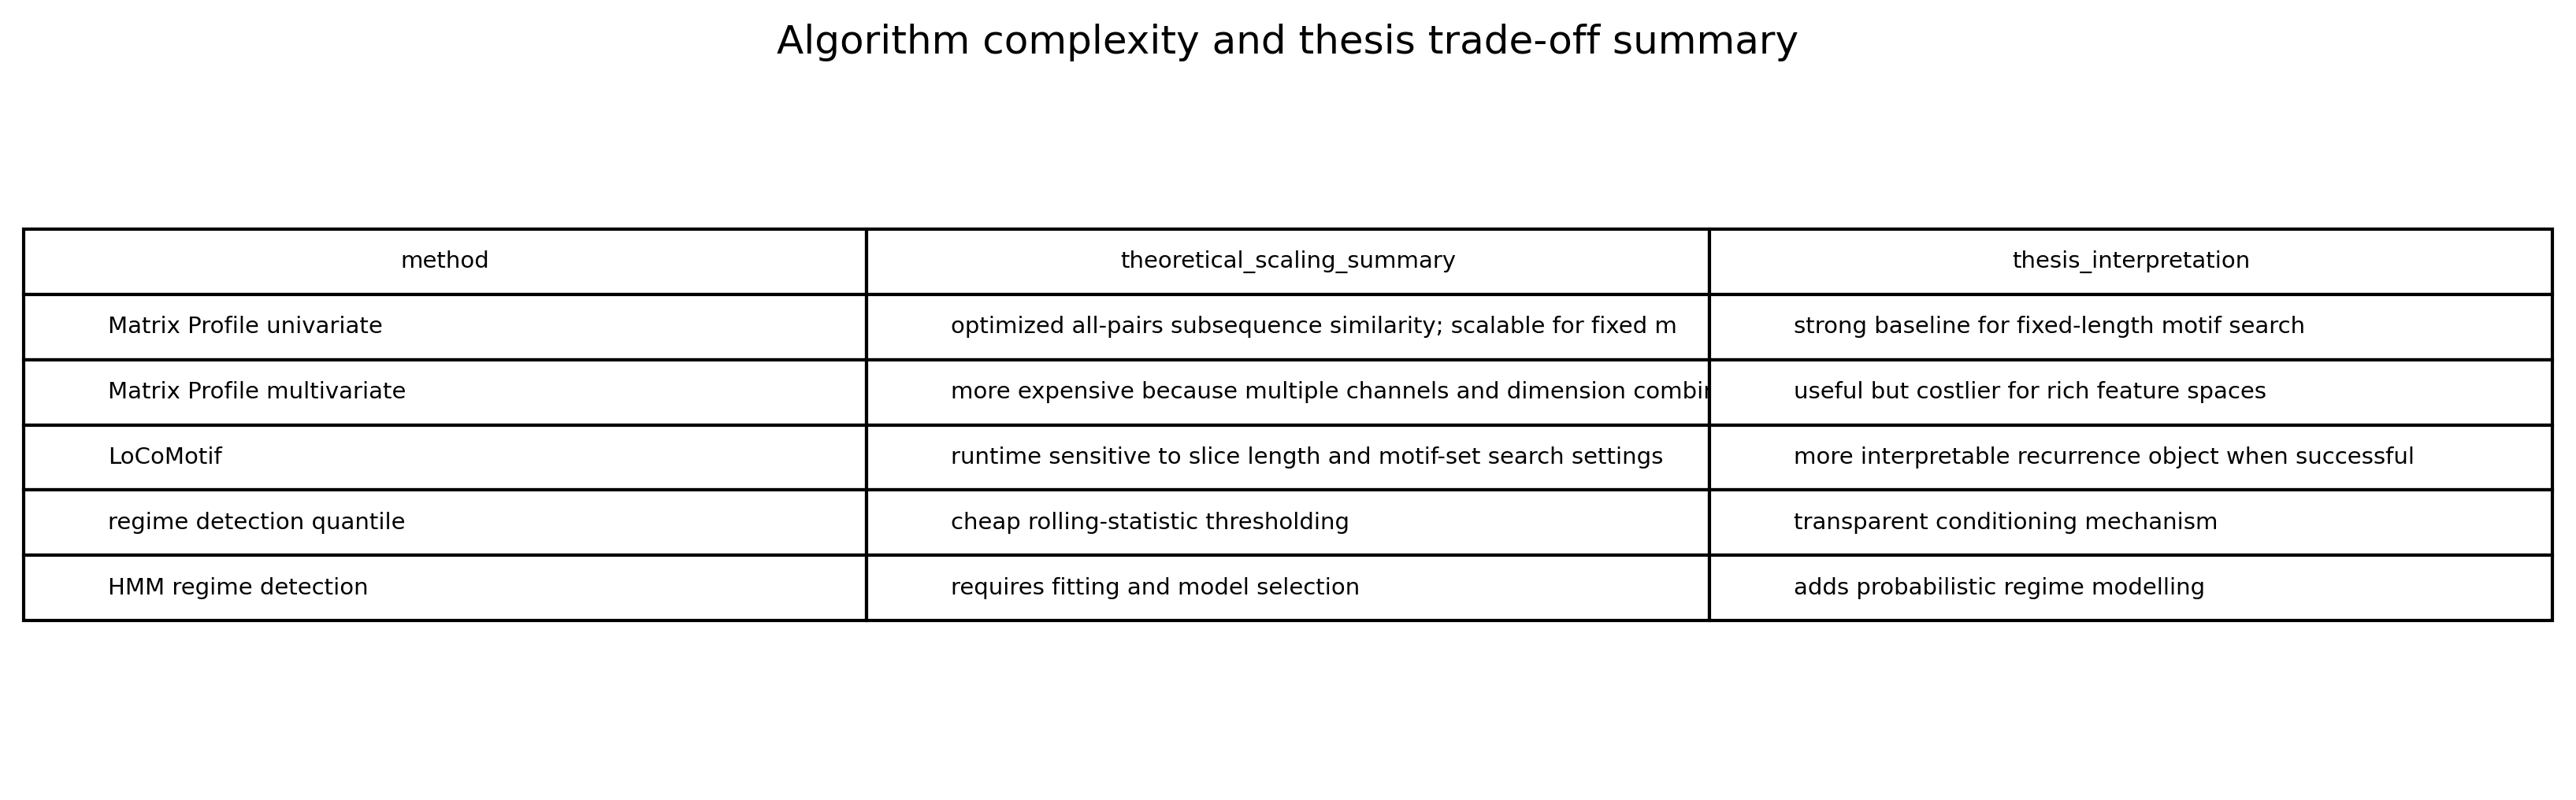
\includegraphics[width=0.9\linewidth]{reports/final_visual_evidence/figures/algorithm_complexity_tradeoff_summary.png}
\caption{algorithm complexity tradeoff summary.}
\end{figure}

\begin{figure}[ht]
\centering
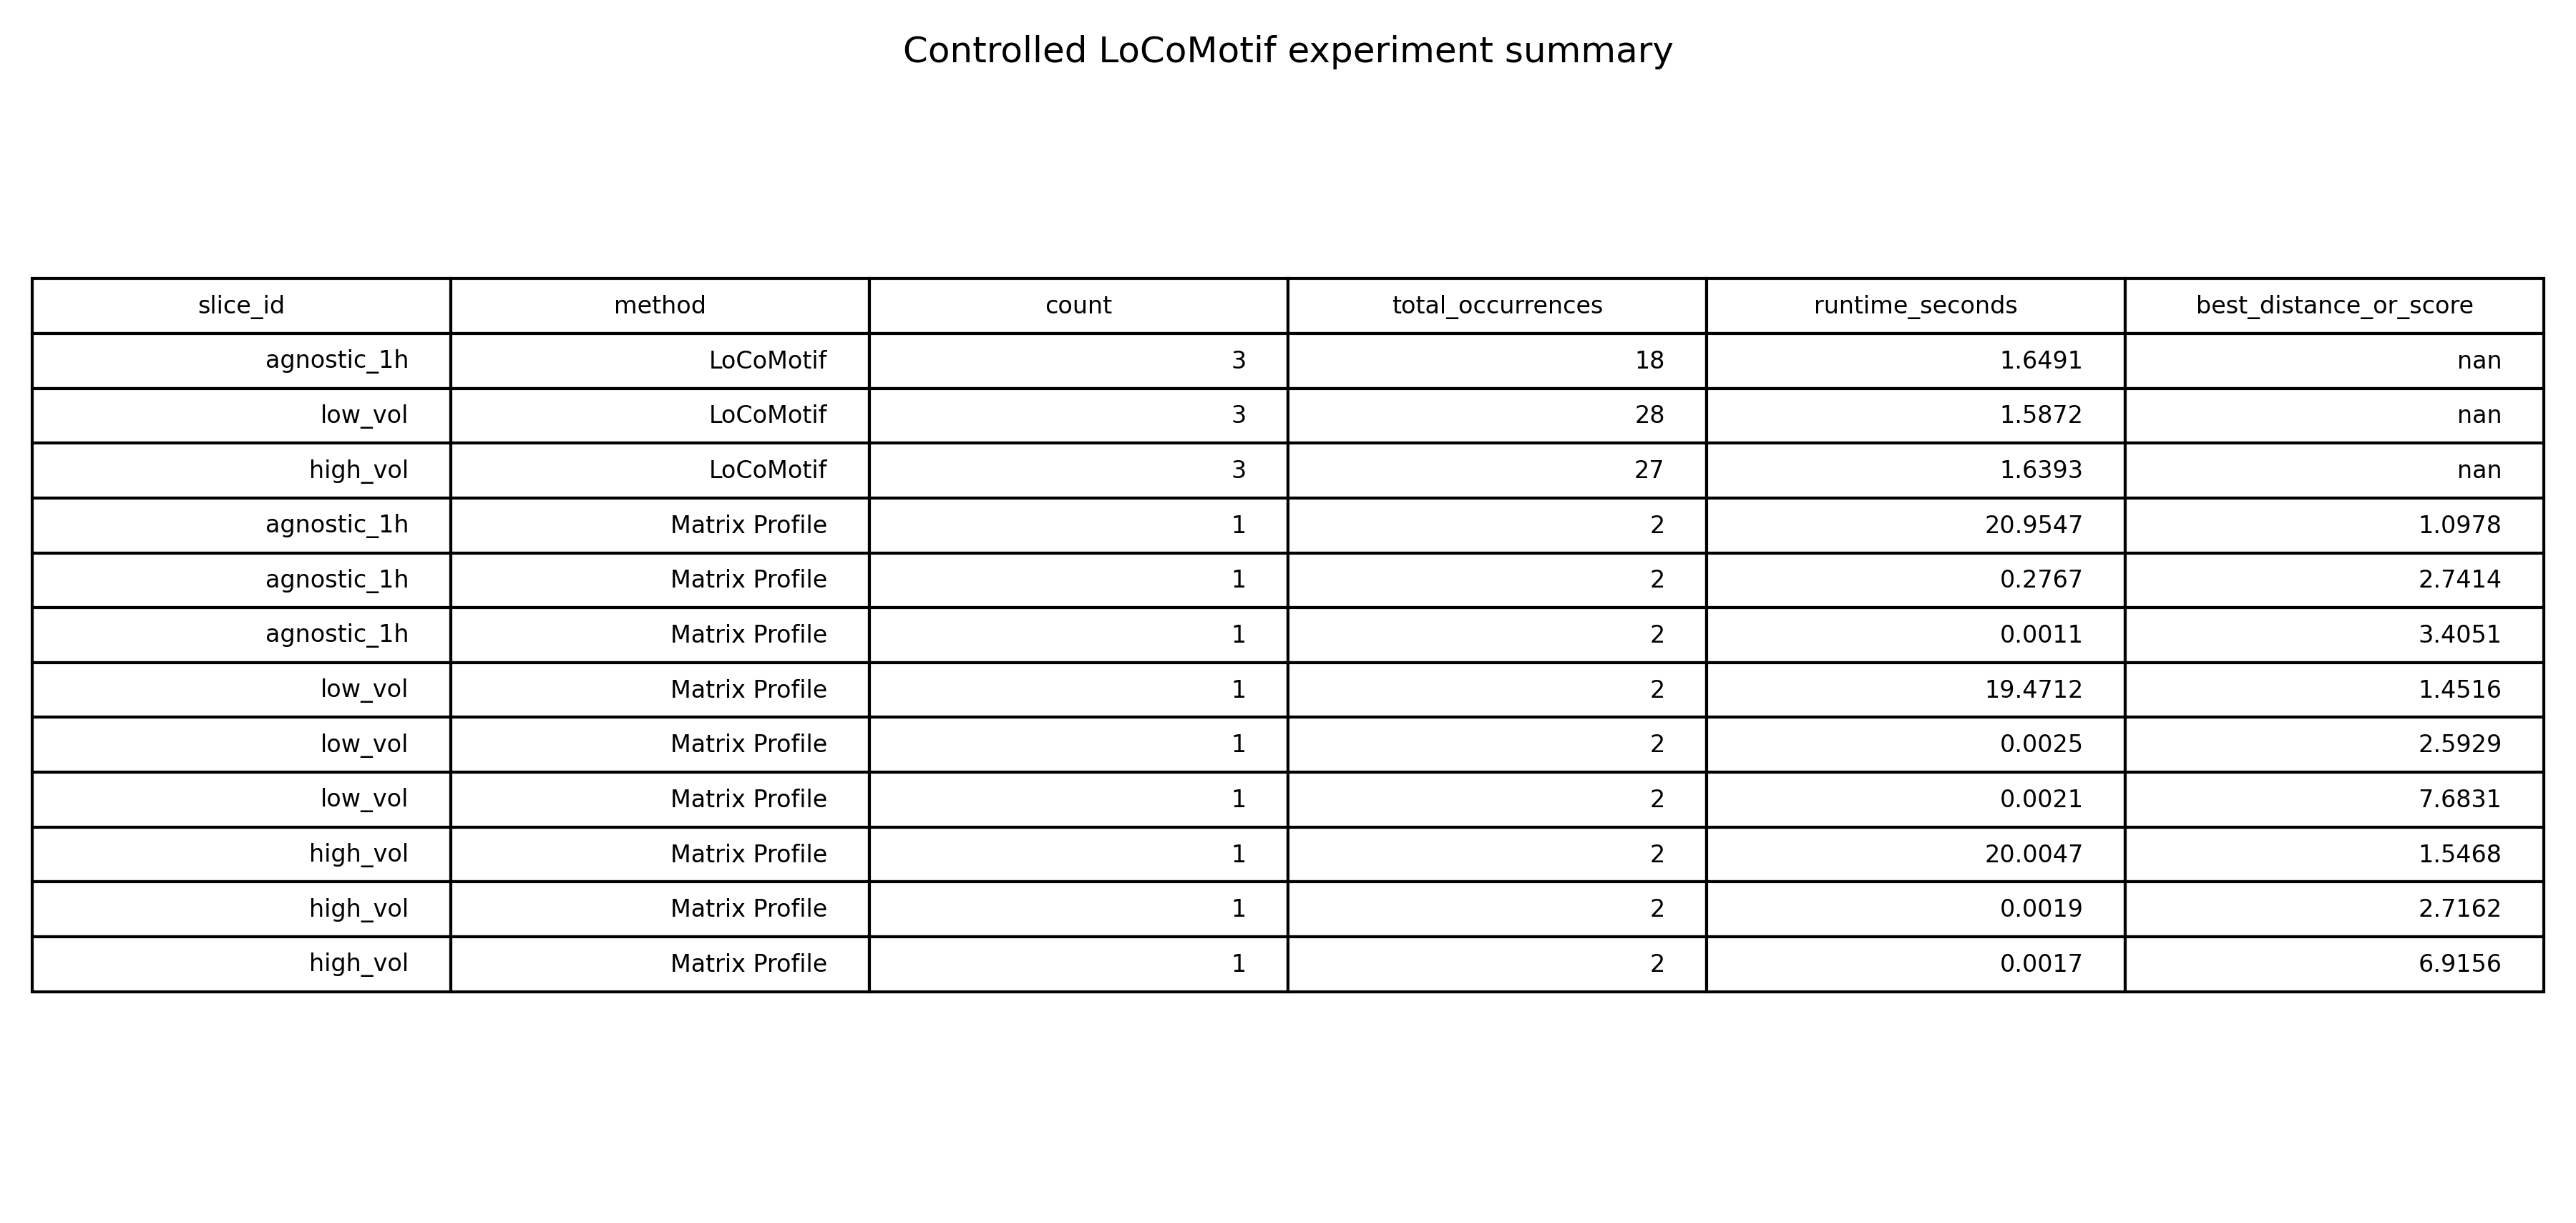
\includegraphics[width=0.9\linewidth]{reports/final_visual_evidence/figures/final_locomotif_controlled_summary.png}
\caption{final locomotif controlled summary. The figure compares real available Matrix Profile and LoCoMotif outputs while preserving object-type differences.}
\end{figure}

\begin{figure}[ht]
\centering
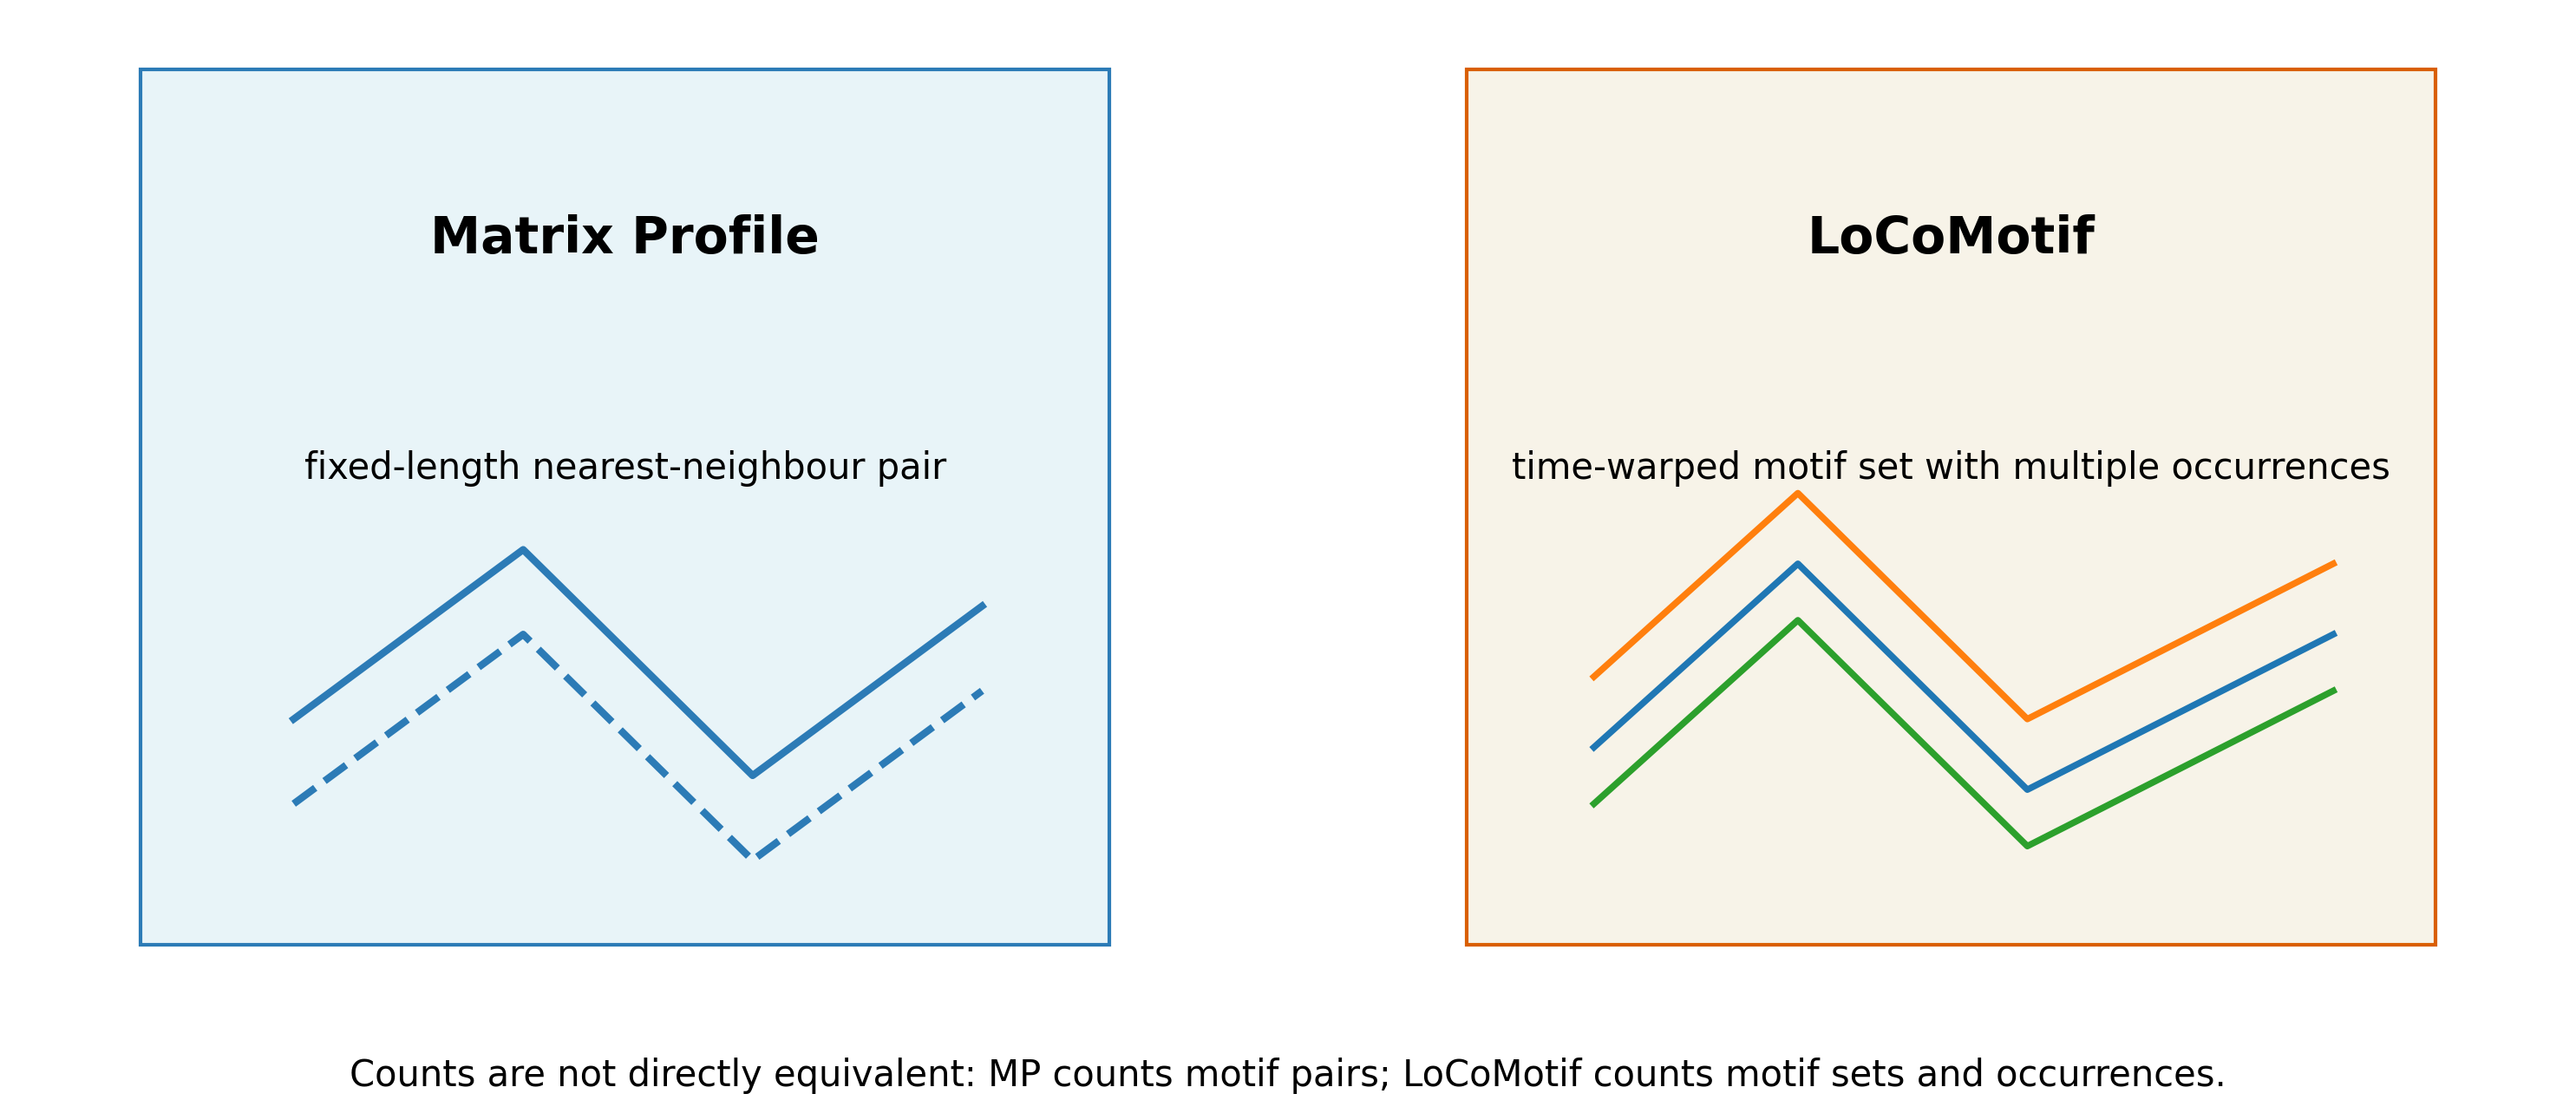
\includegraphics[width=0.9\linewidth]{reports/final_visual_evidence/figures/final_method_object_comparison_diagram.png}
\caption{final method object comparison diagram.}
\end{figure}

\begin{figure}[ht]
\centering
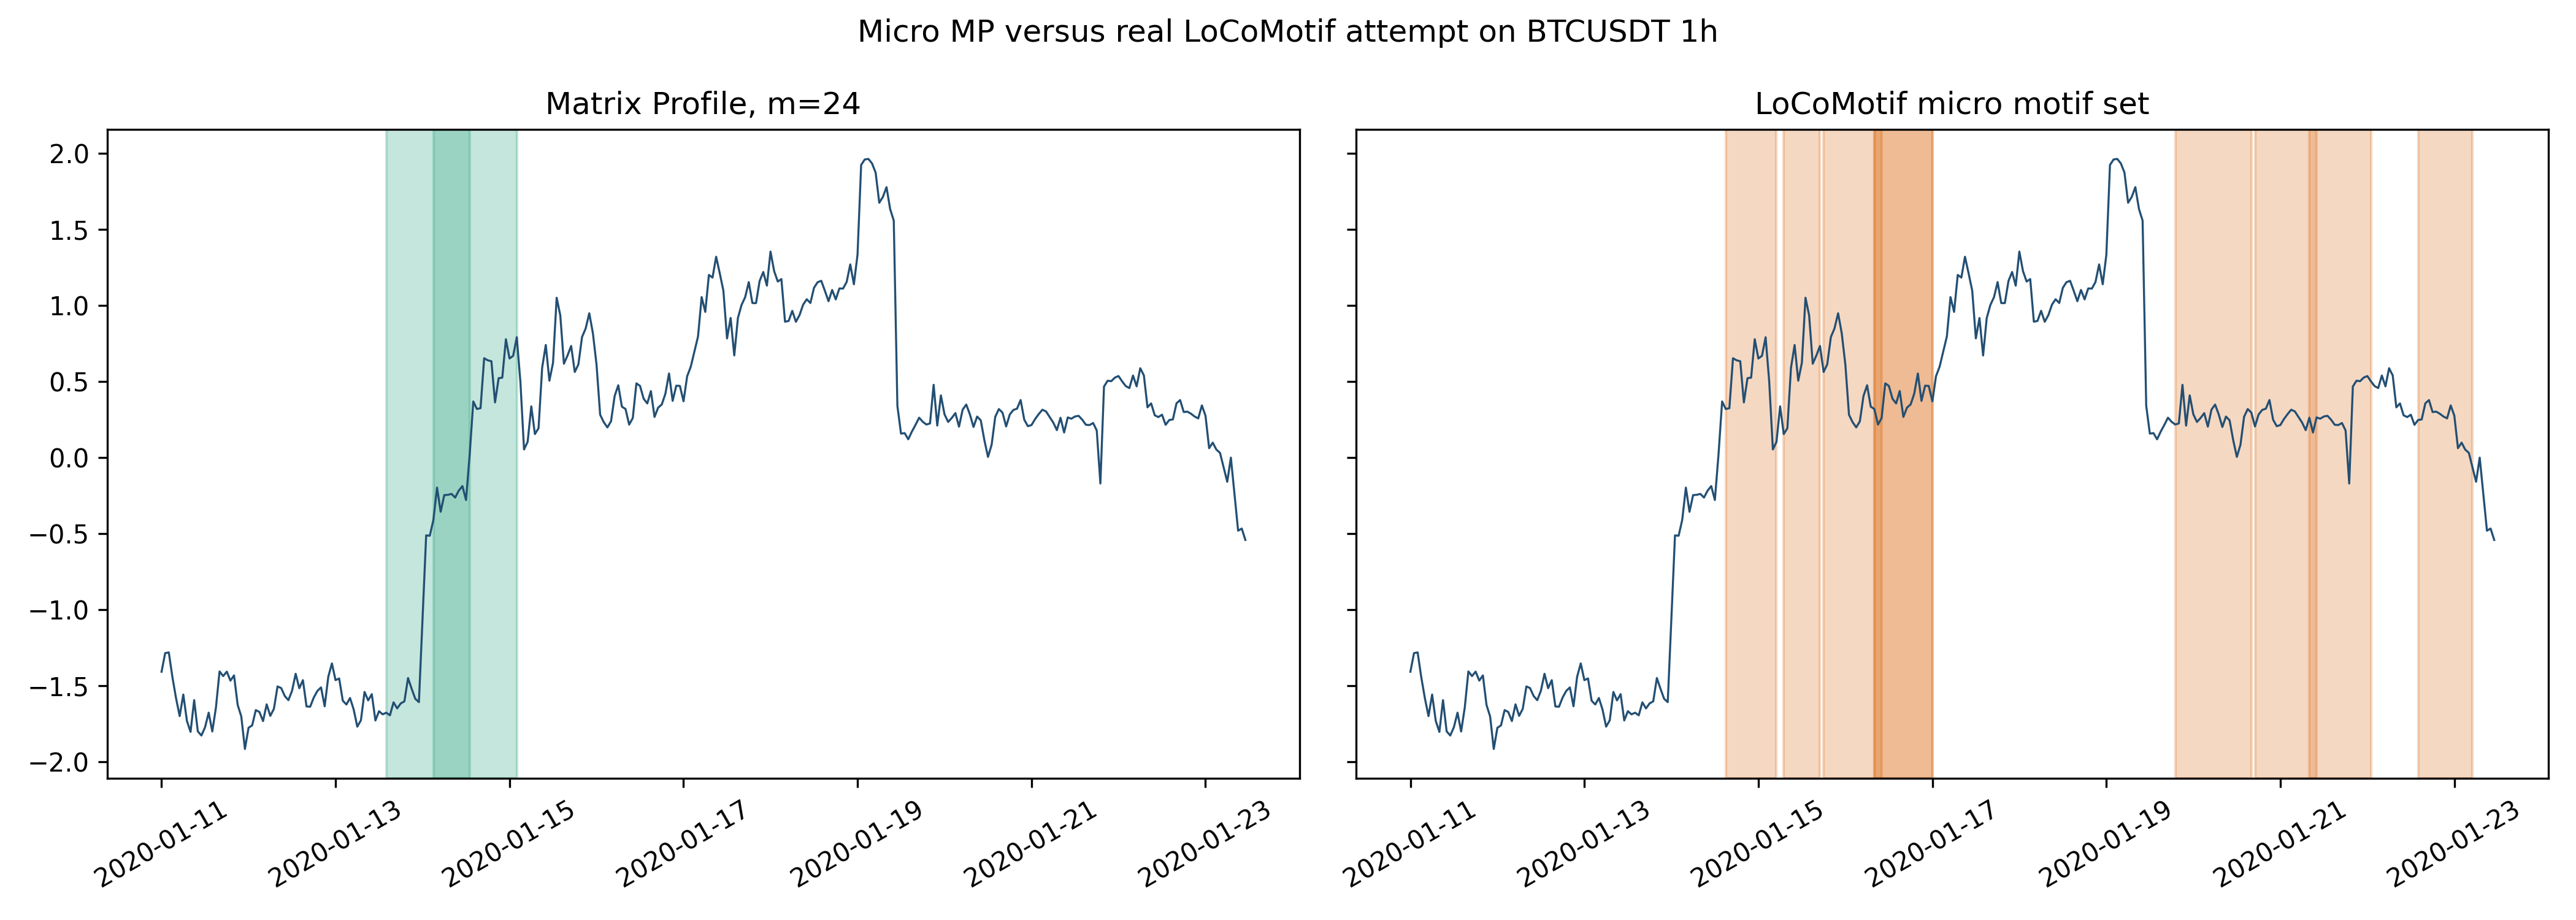
\includegraphics[width=0.9\linewidth]{reports/final_visual_evidence/figures/final_mp_vs_locomotif_agnostic_1h_side_by_side.png}
\caption{final mp vs locomotif agnostic 1h side by side. The figure compares real available Matrix Profile and LoCoMotif outputs while preserving object-type differences.}
\end{figure}

\begin{figure}[ht]
\centering
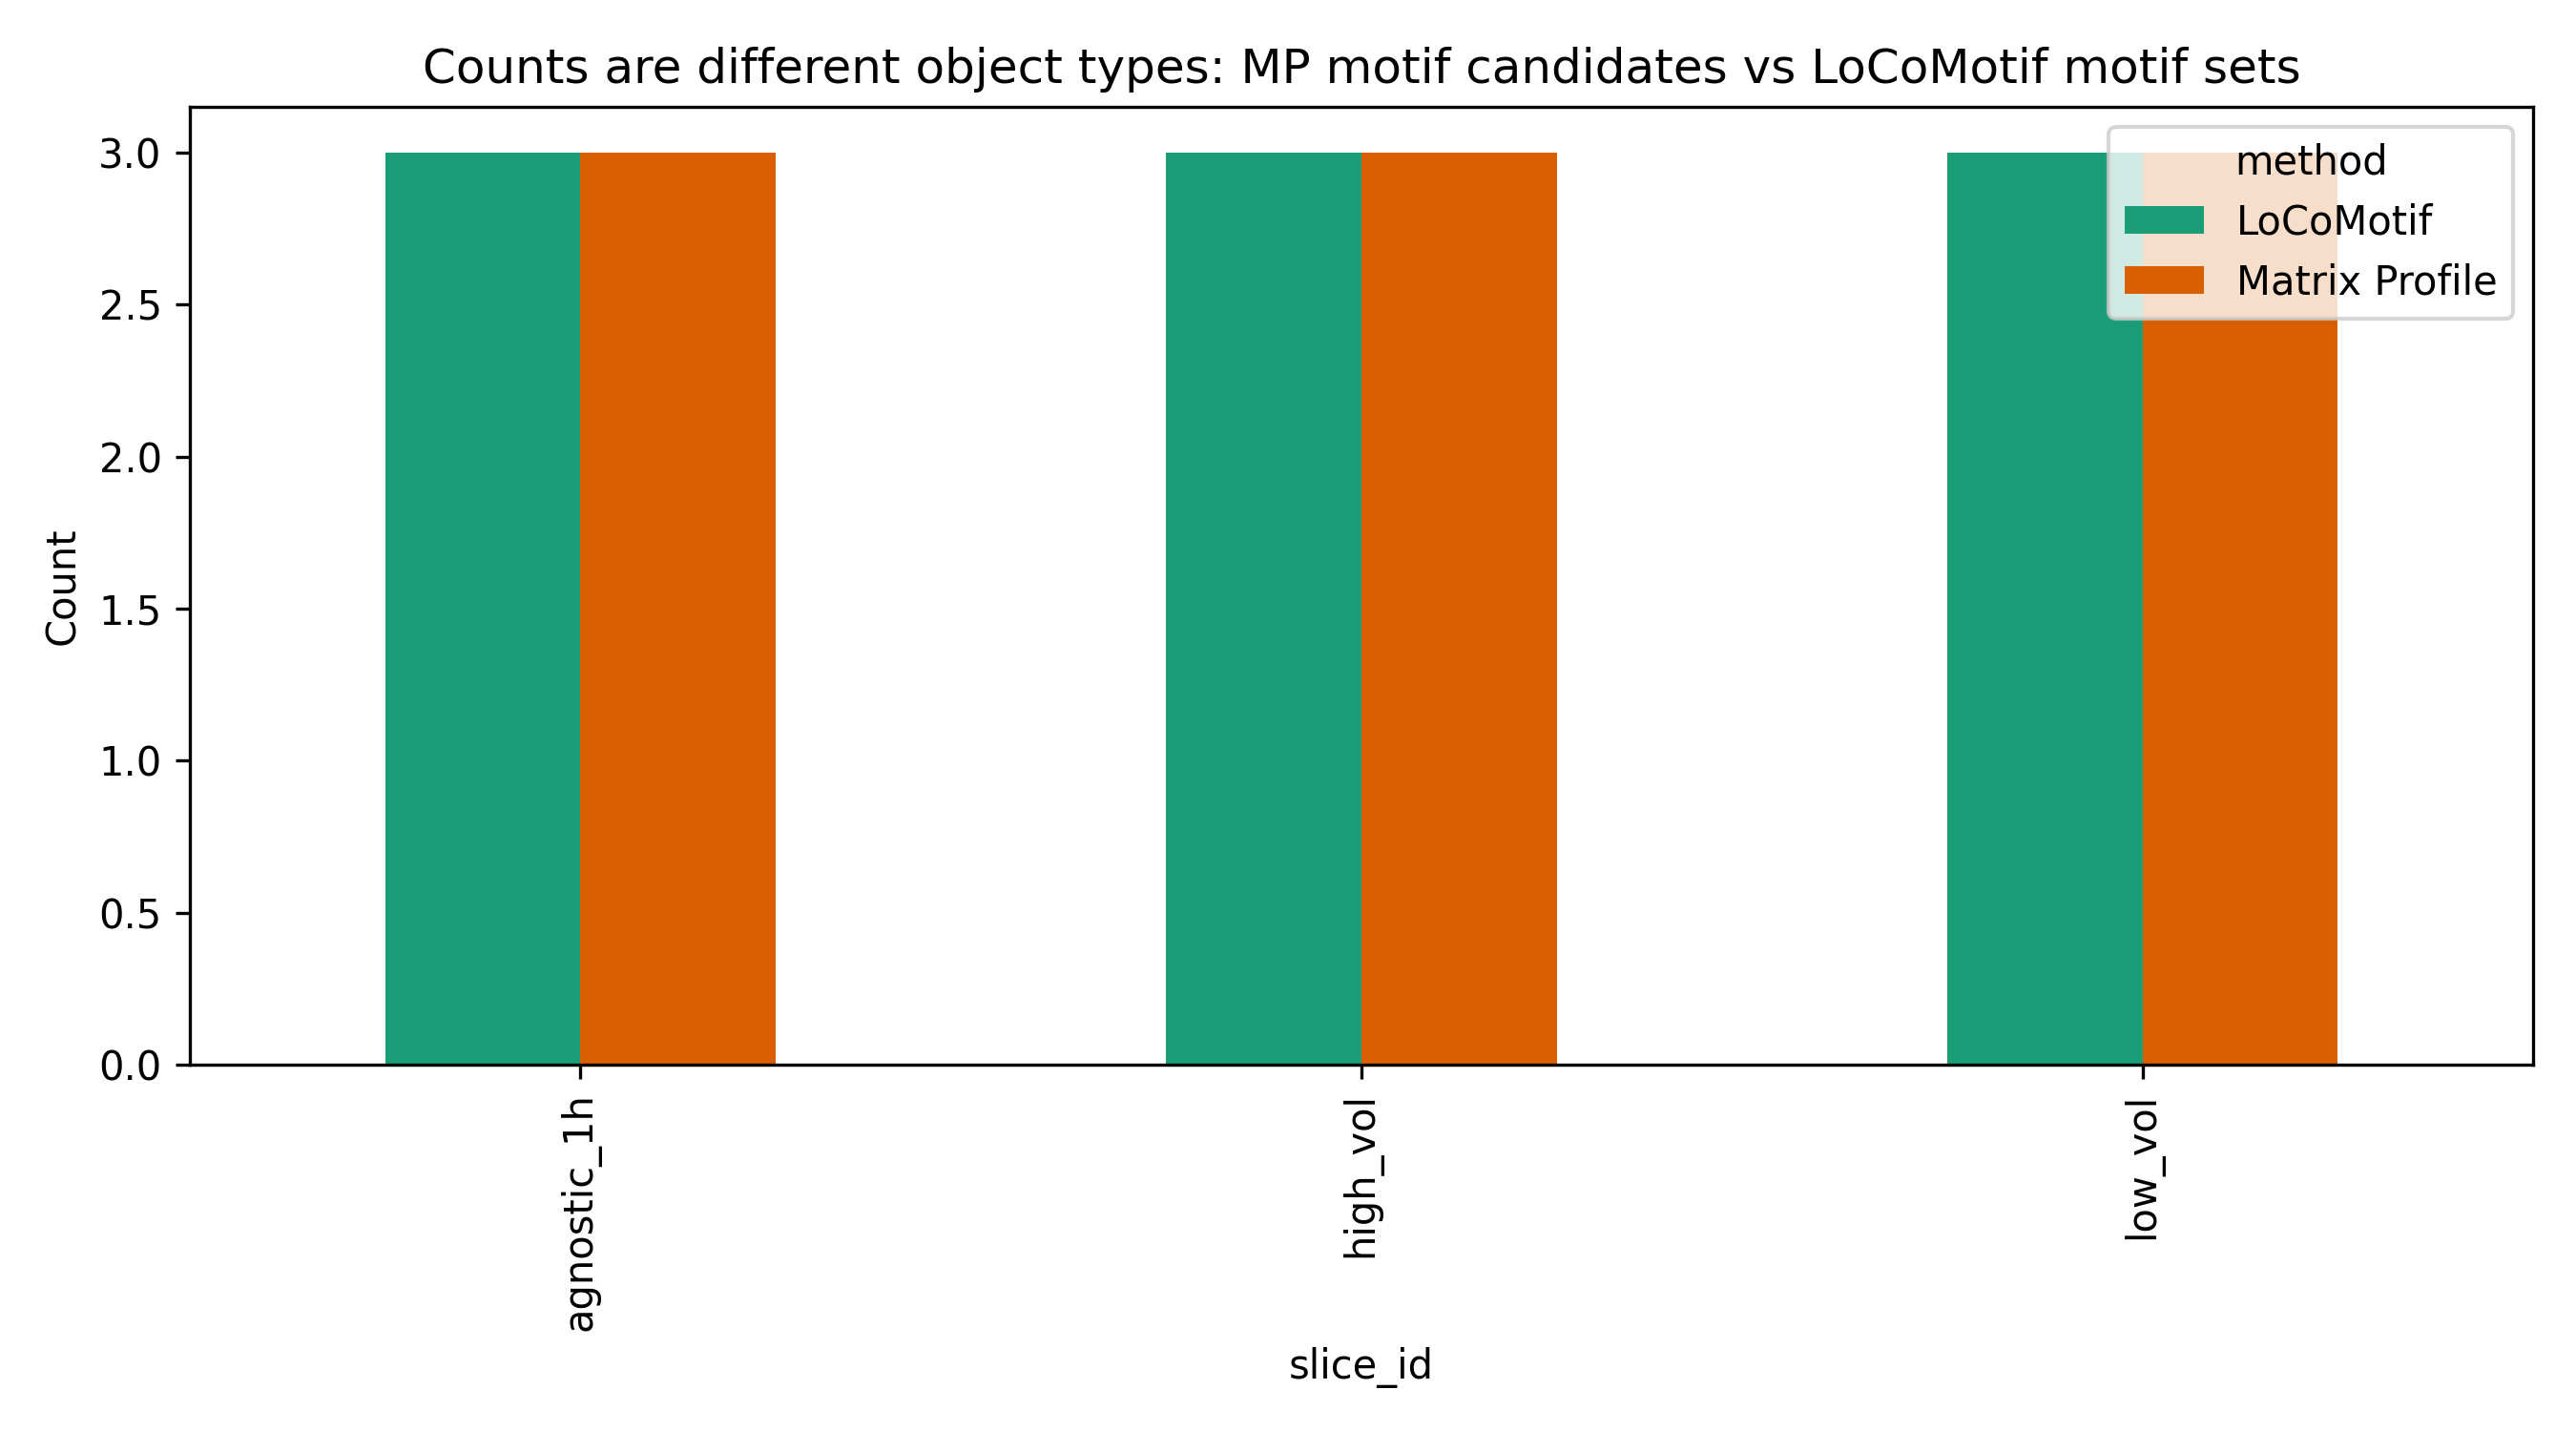
\includegraphics[width=0.9\linewidth]{reports/final_visual_evidence/figures/final_mp_vs_locomotif_counts_and_occurrences.png}
\caption{final mp vs locomotif counts and occurrences. The figure compares real available Matrix Profile and LoCoMotif outputs while preserving object-type differences.}
\end{figure}

\begin{figure}[ht]
\centering
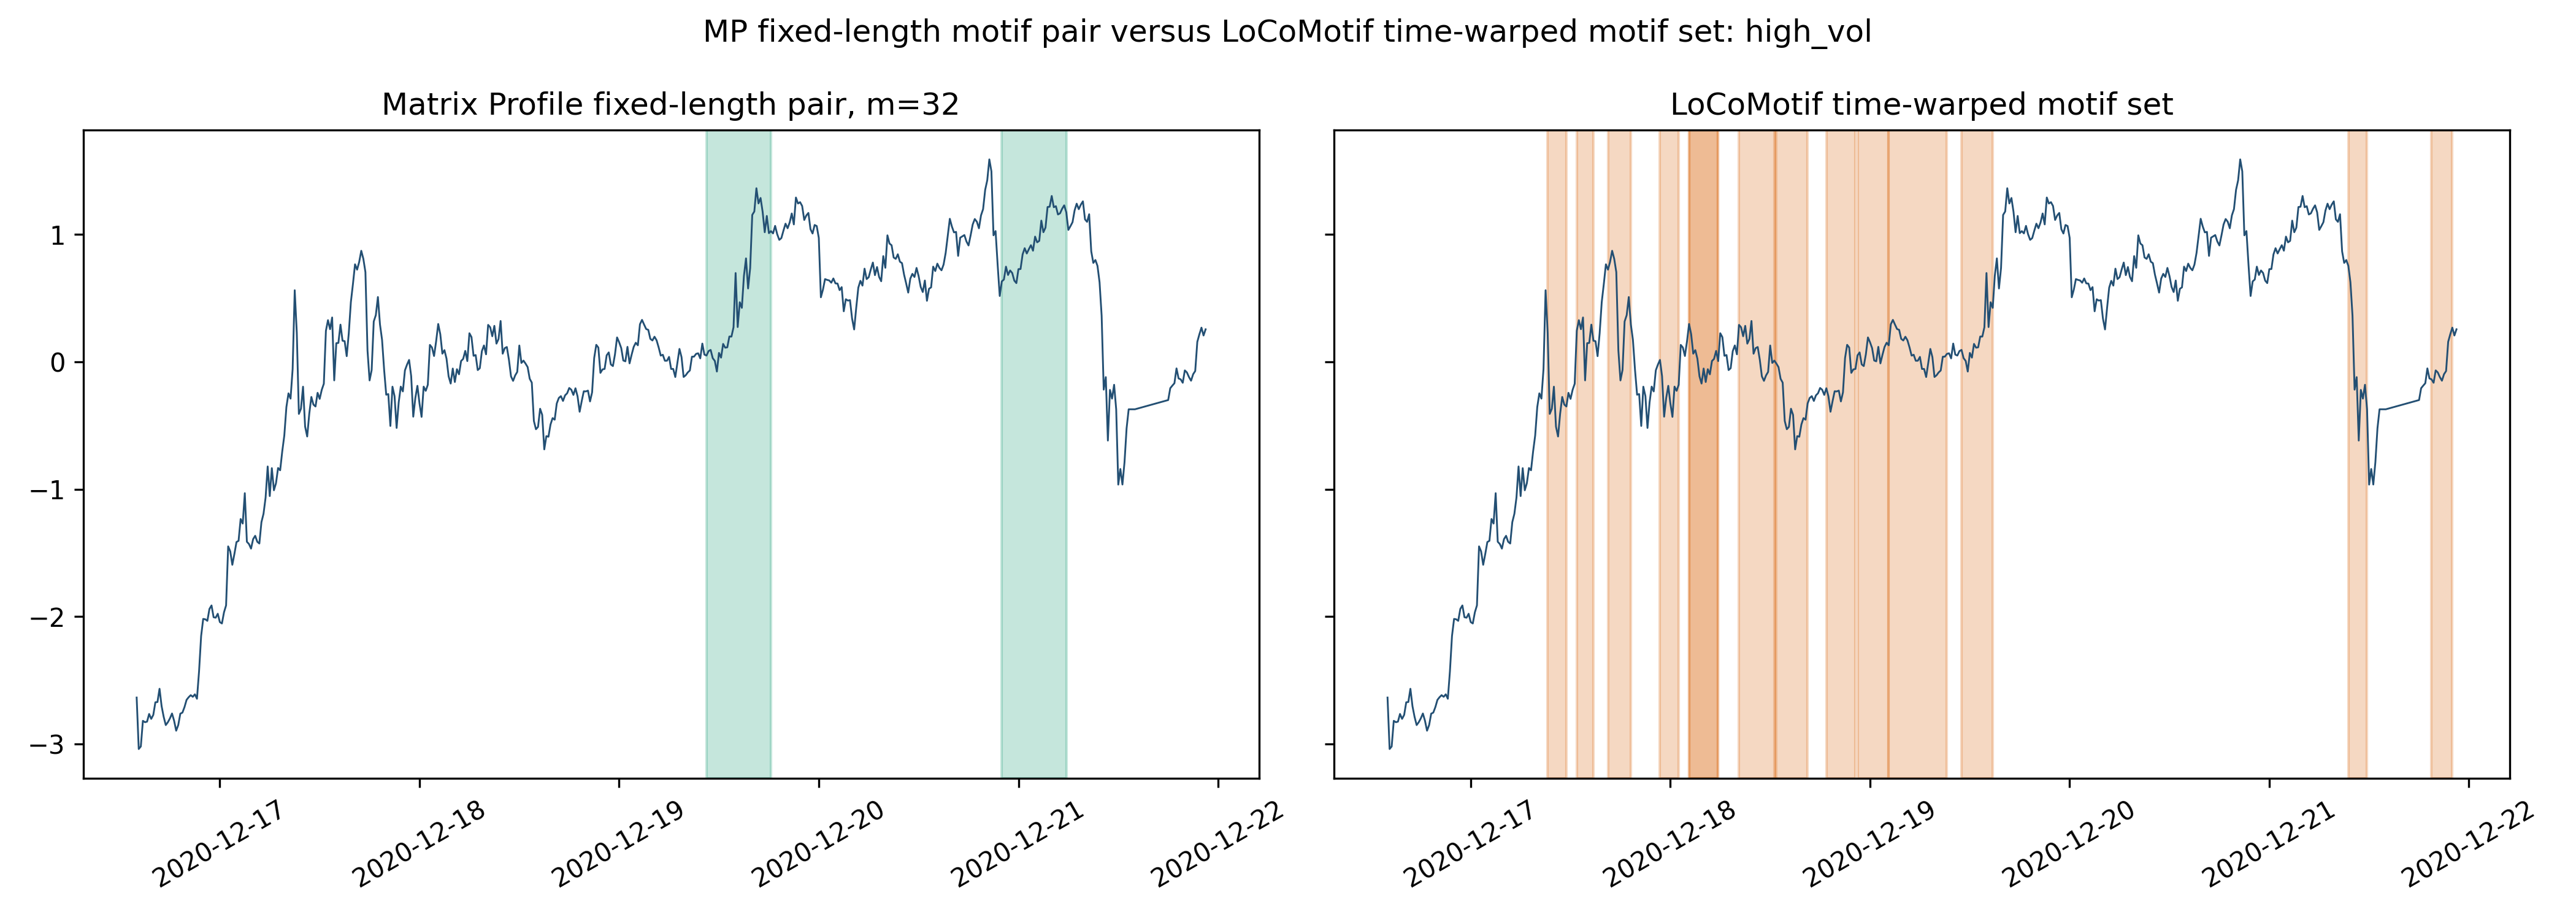
\includegraphics[width=0.9\linewidth]{reports/final_visual_evidence/figures/final_mp_vs_locomotif_high_vol_side_by_side.png}
\caption{final mp vs locomotif high vol side by side. The figure compares real available Matrix Profile and LoCoMotif outputs while preserving object-type differences.}
\end{figure}

\begin{figure}[ht]
\centering
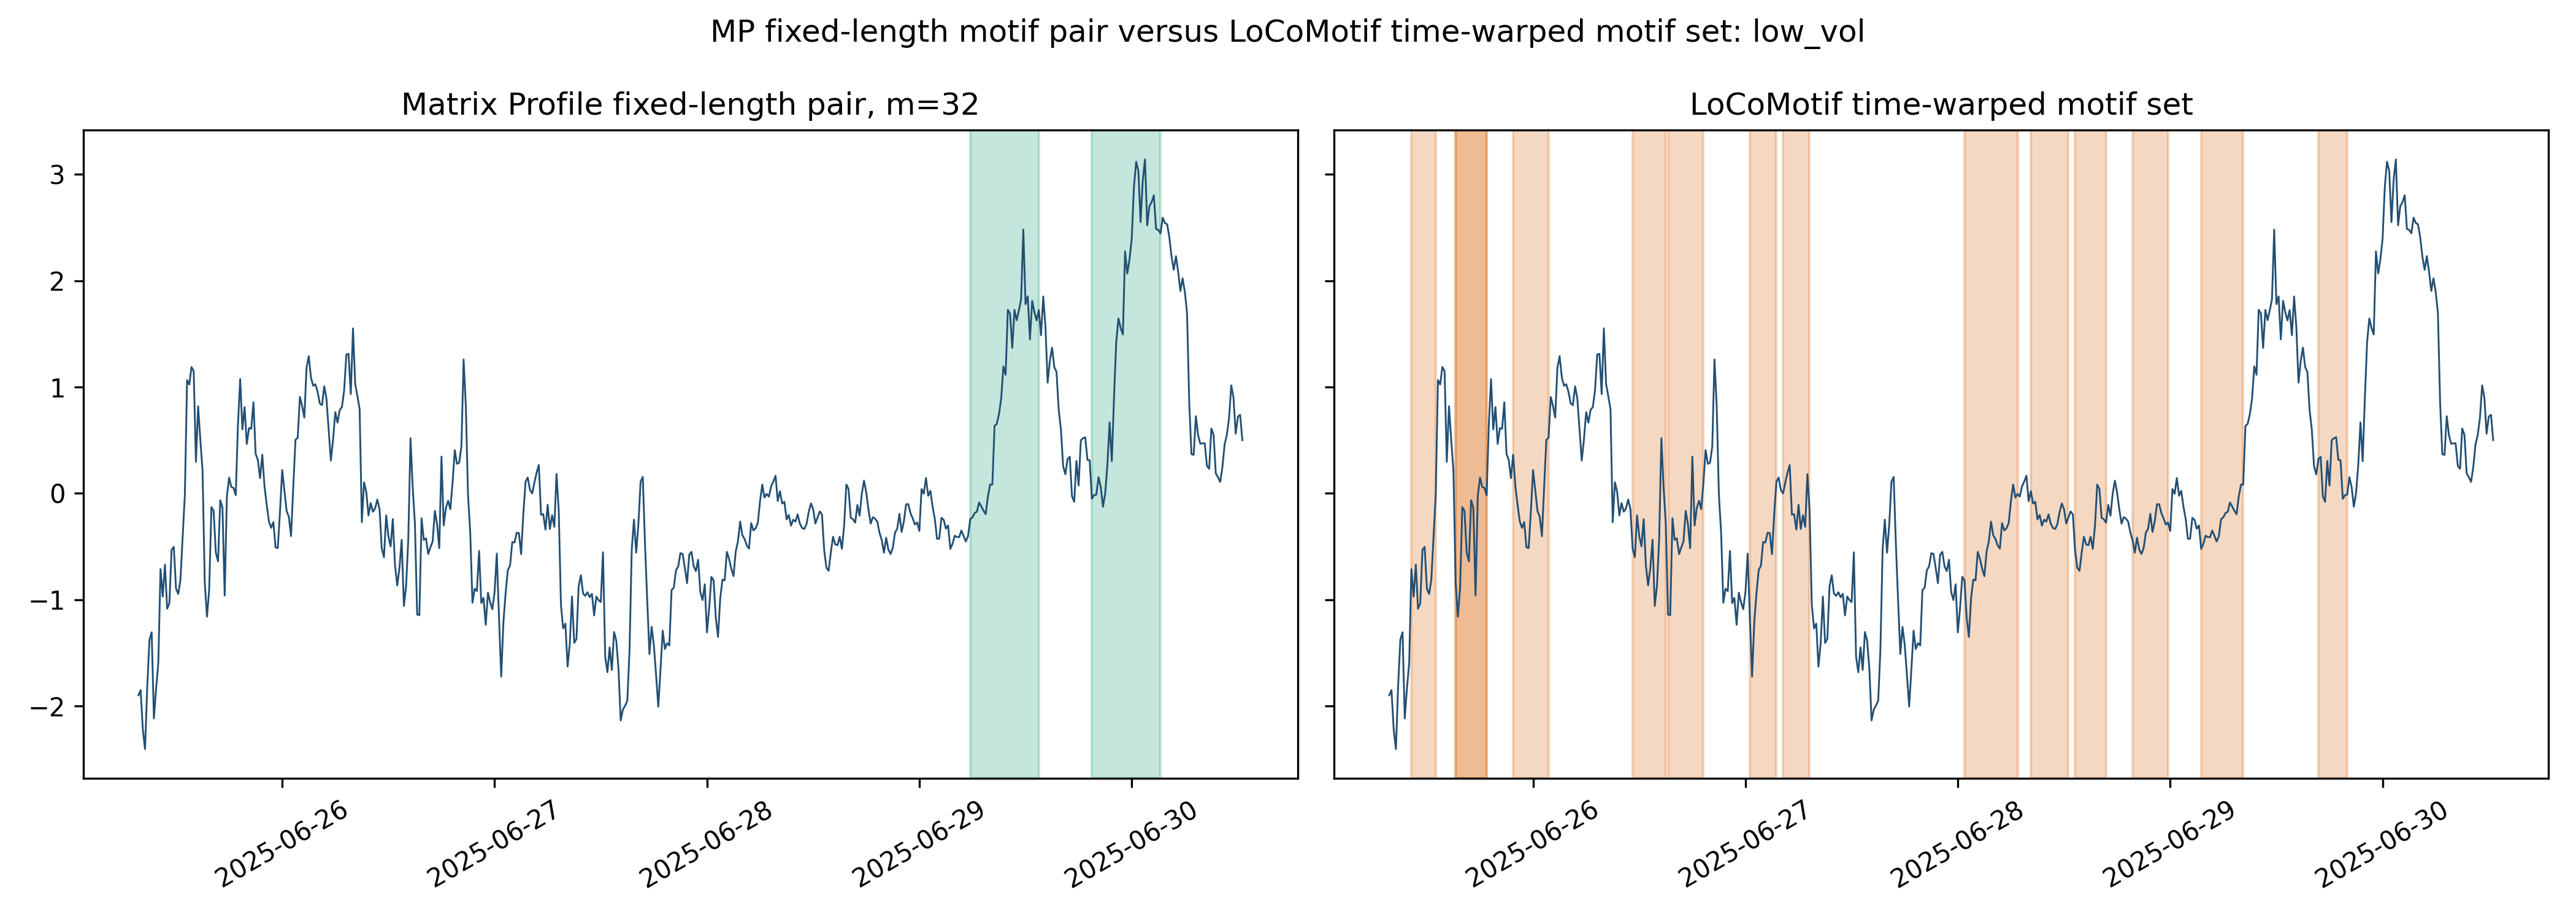
\includegraphics[width=0.9\linewidth]{reports/final_visual_evidence/figures/final_mp_vs_locomotif_low_vol_side_by_side.png}
\caption{final mp vs locomotif low vol side by side. The figure compares real available Matrix Profile and LoCoMotif outputs while preserving object-type differences.}
\end{figure}

\begin{figure}[ht]
\centering
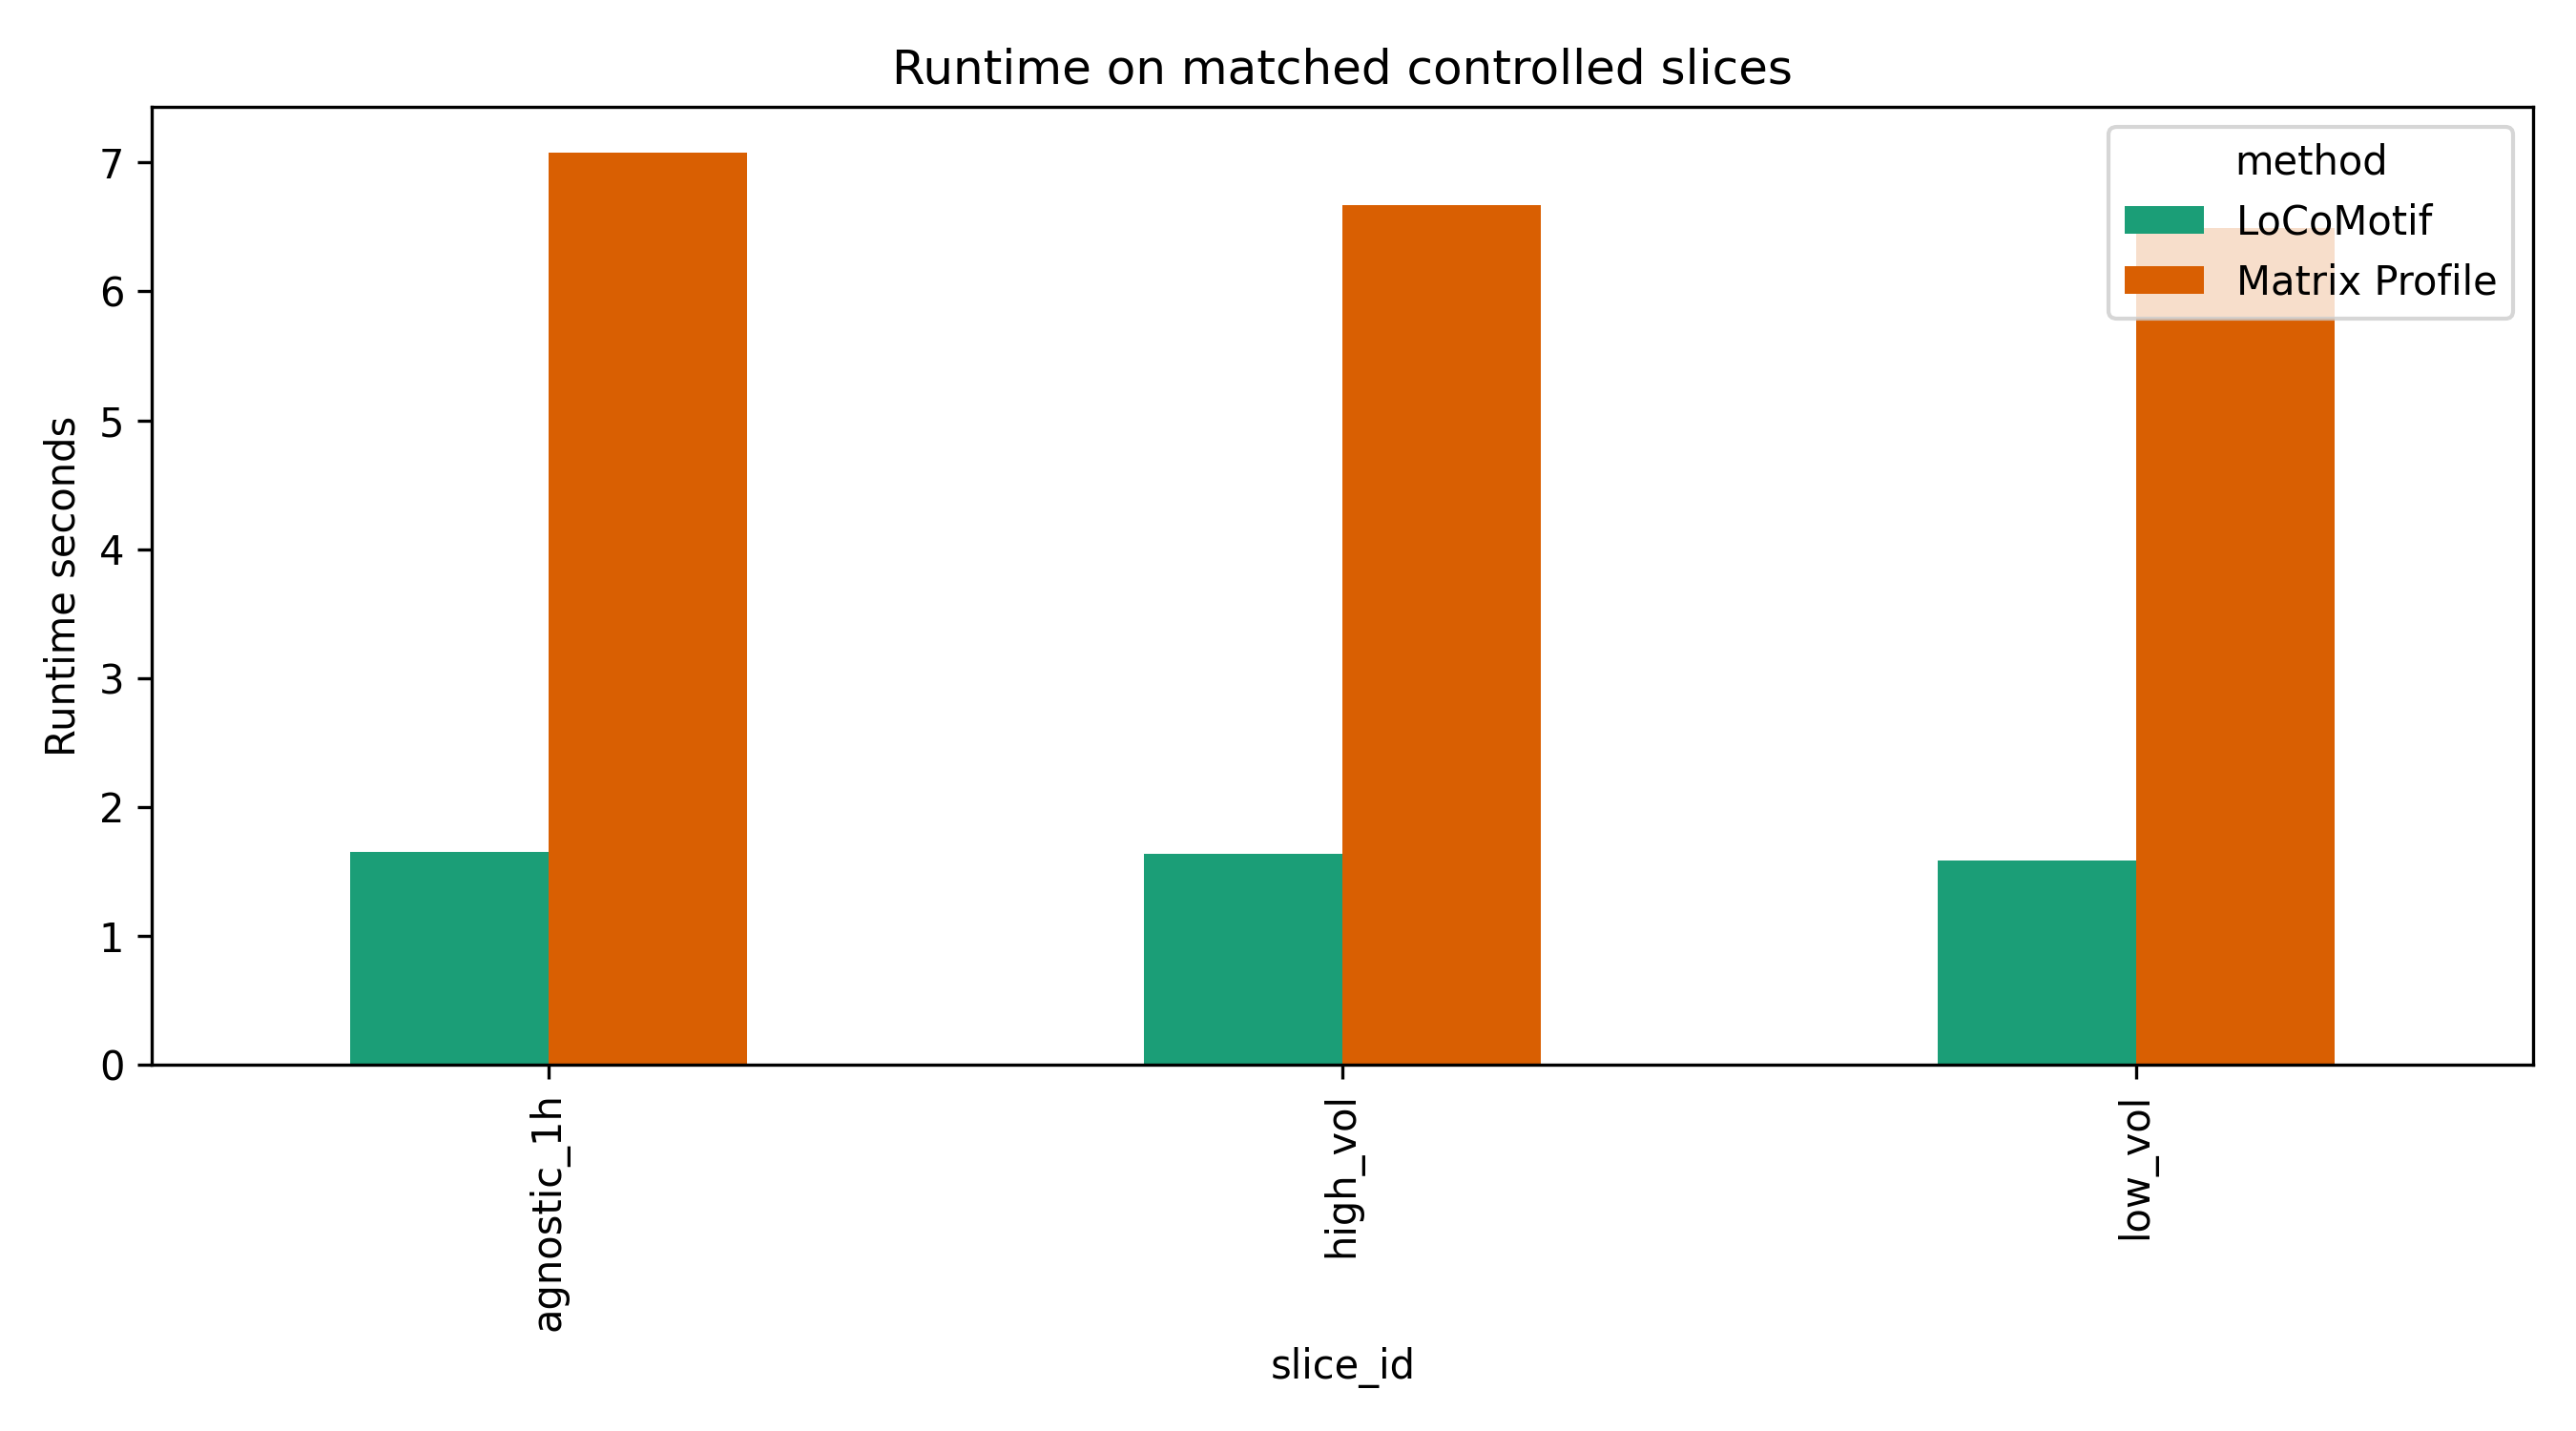
\includegraphics[width=0.9\linewidth]{reports/final_visual_evidence/figures/final_mp_vs_locomotif_runtime.png}
\caption{final mp vs locomotif runtime. The figure compares real available Matrix Profile and LoCoMotif outputs while preserving object-type differences.}
\end{figure}

\begin{figure}[ht]
\centering
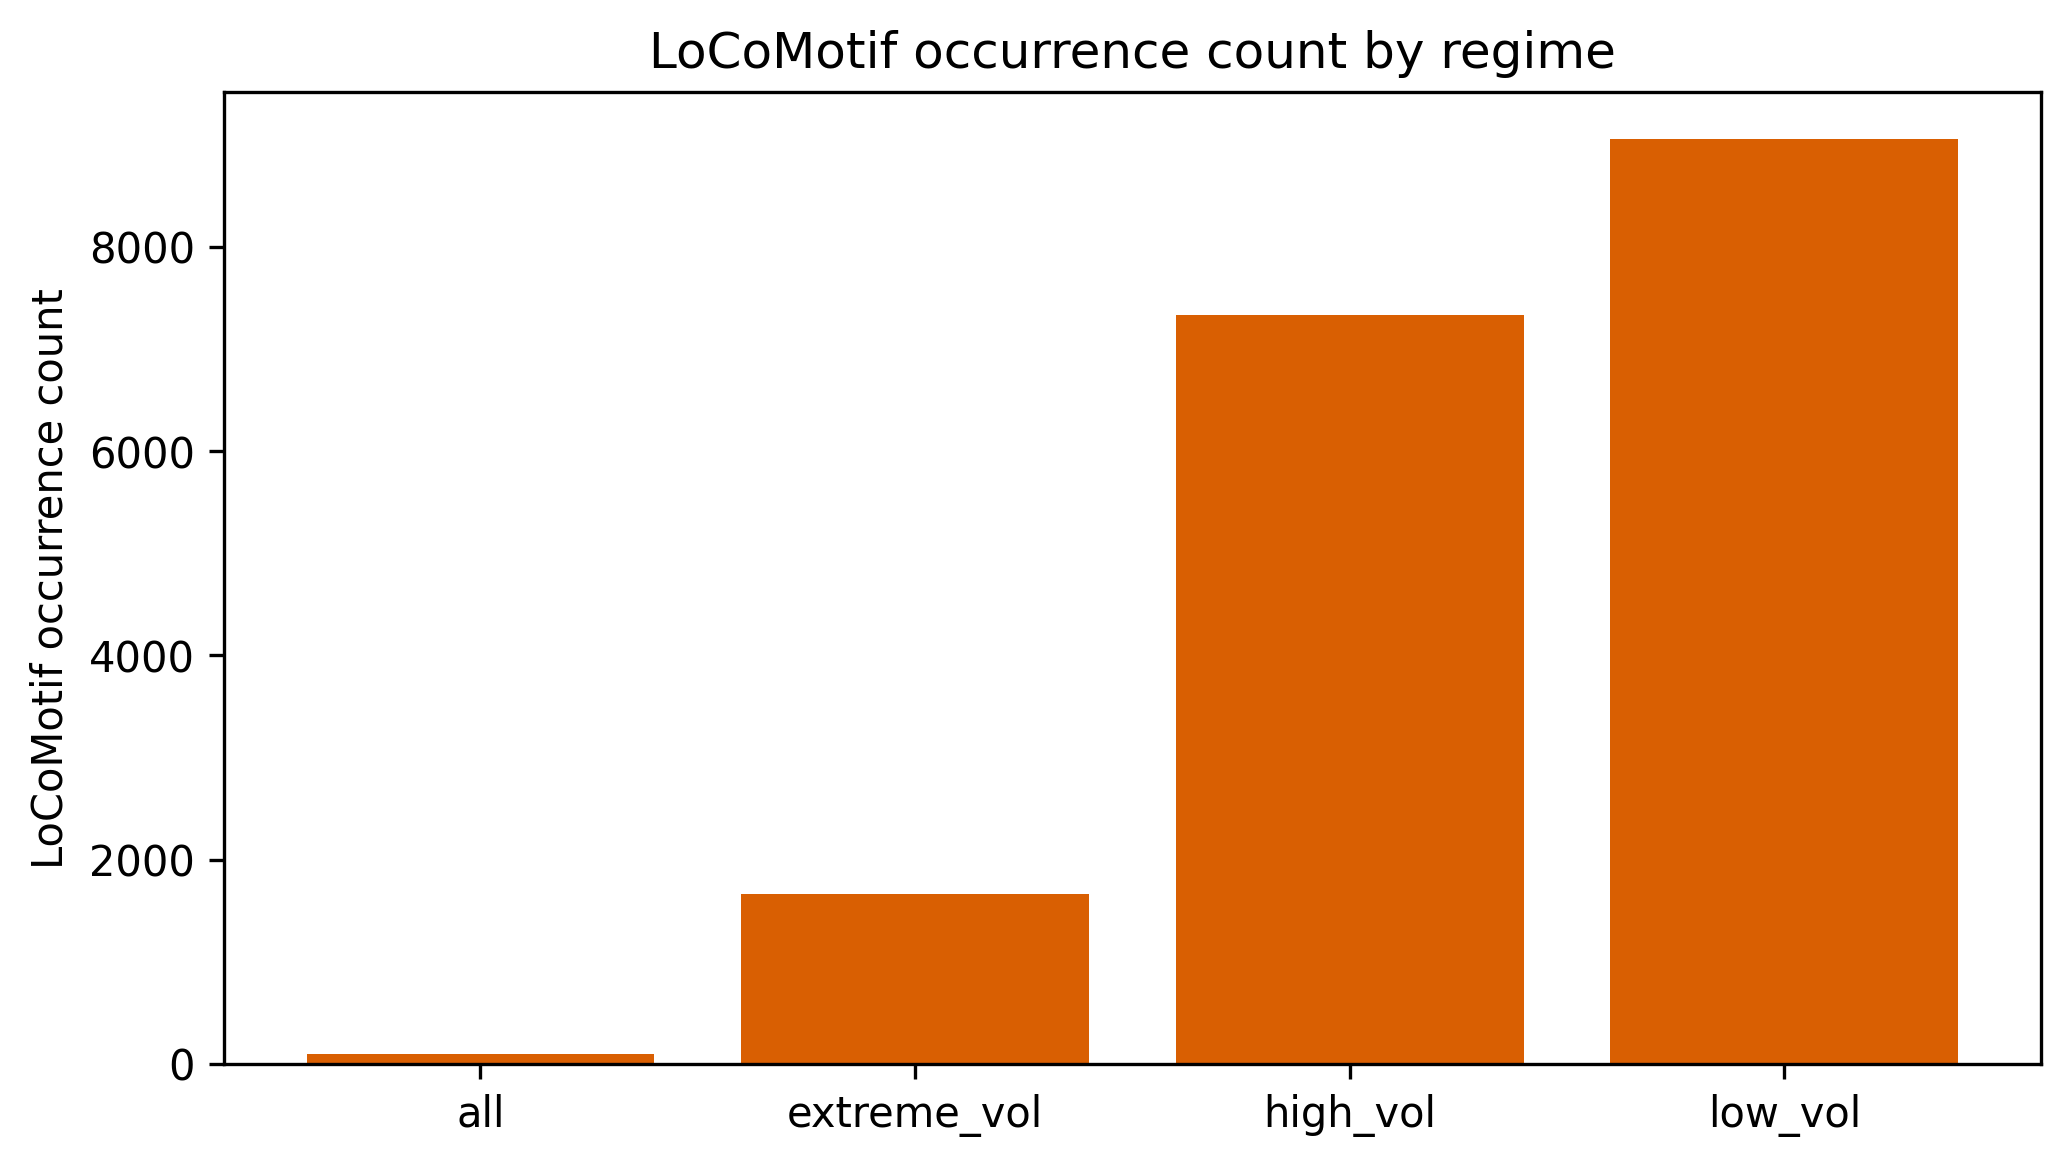
\includegraphics[width=0.9\linewidth]{reports/final_visual_evidence/figures/loco_occurrence_count_by_regime.png}
\caption{loco occurrence count by regime.}
\end{figure}

\begin{figure}[ht]
\centering
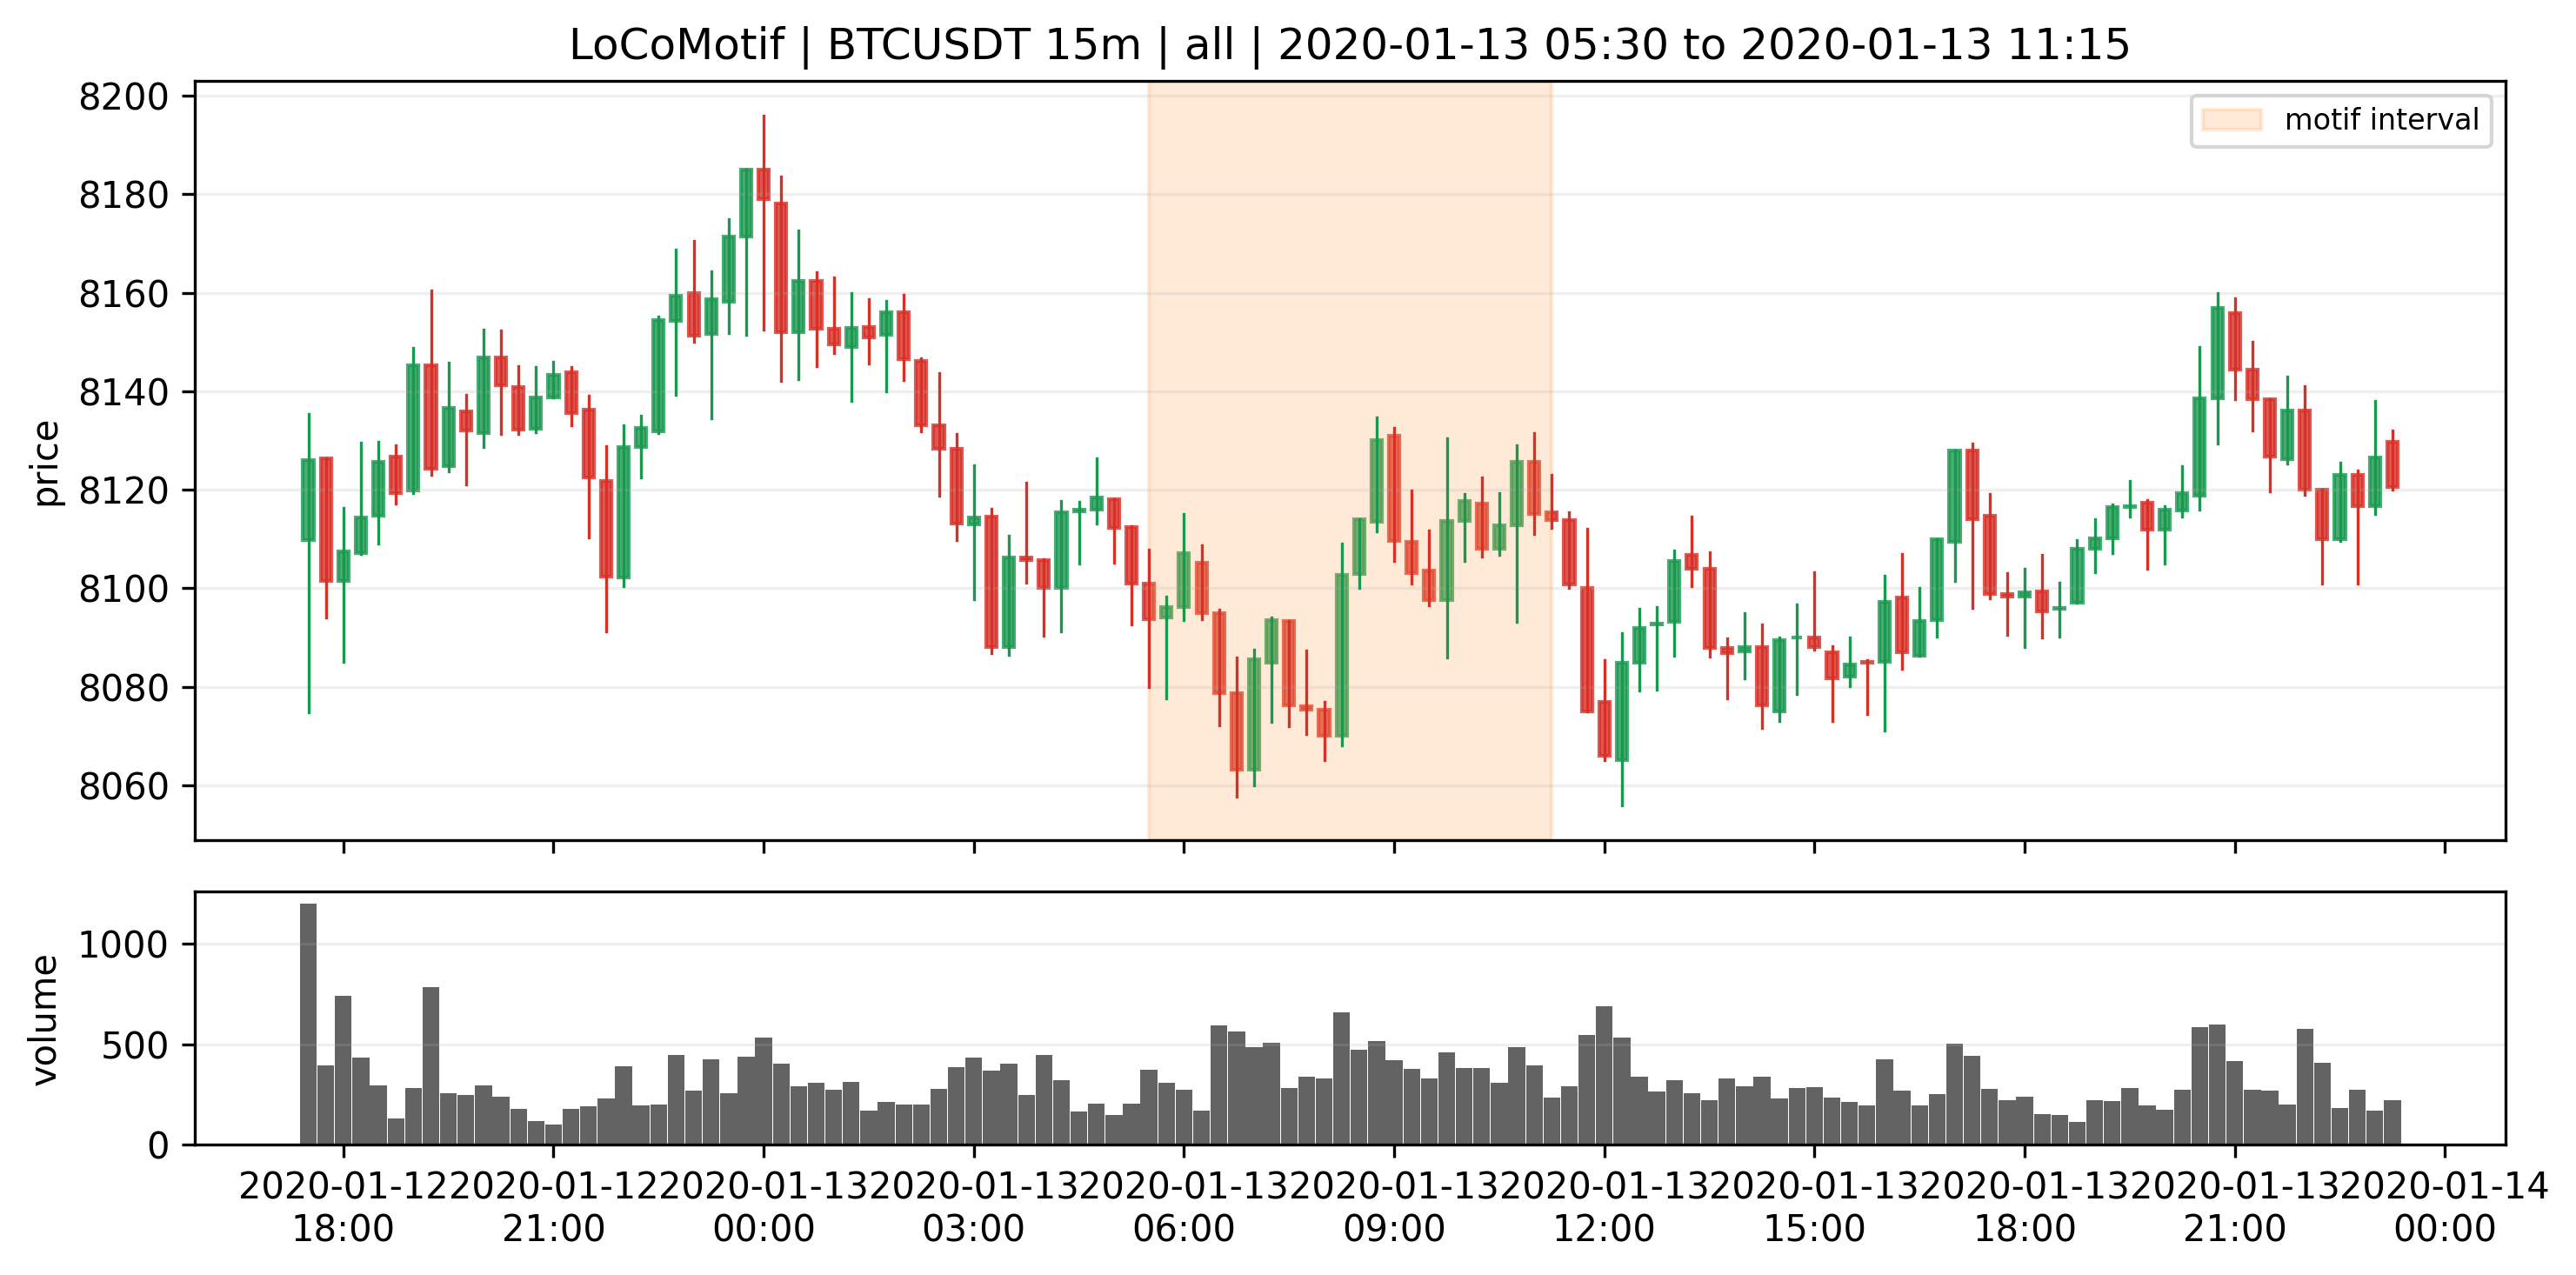
\includegraphics[width=0.9\linewidth]{reports/final_visual_evidence/figures/motif_01_locomotif_btcusdt_15m_all_1_0_1_0_context.png}
\caption{motif 01 locomotif btcusdt 15m all 1 0 1 0 context. The figure compares real available Matrix Profile and LoCoMotif outputs while preserving object-type differences.}
\end{figure}

\begin{figure}[ht]
\centering
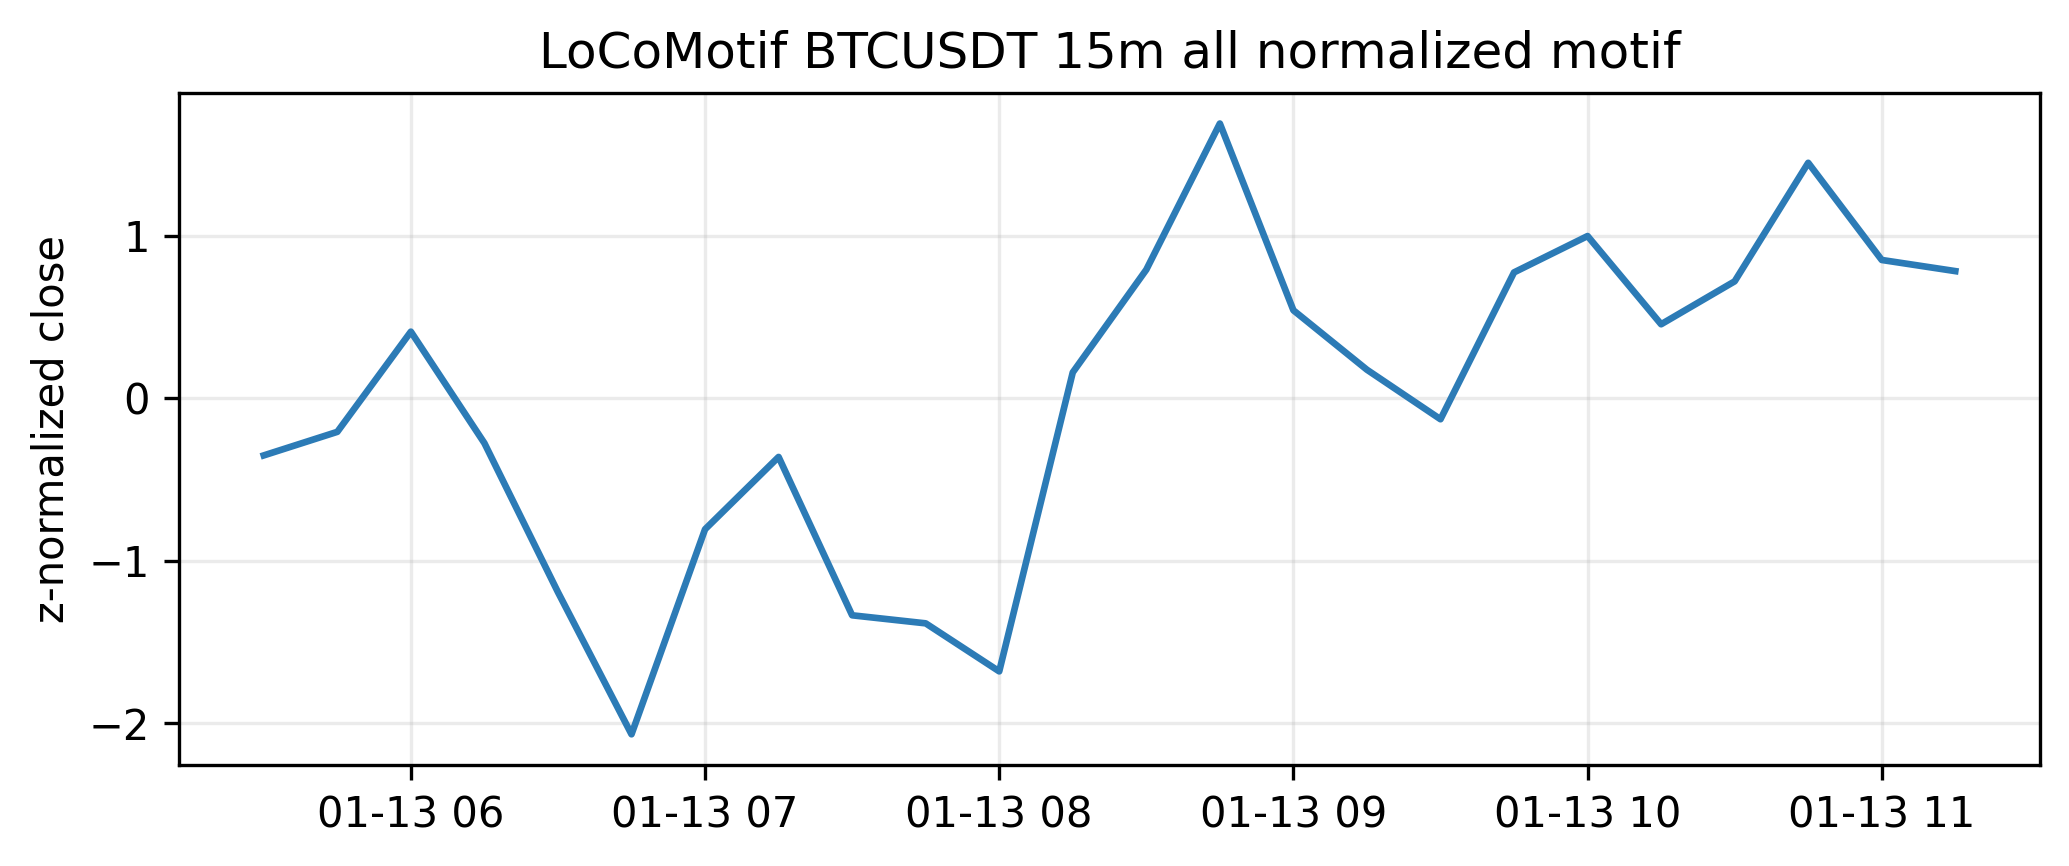
\includegraphics[width=0.9\linewidth]{reports/final_visual_evidence/figures/motif_01_locomotif_btcusdt_15m_all_1_0_1_0_normal_pattern.png}
\caption{motif 01 locomotif btcusdt 15m all 1 0 1 0 normal pattern. The figure compares real available Matrix Profile and LoCoMotif outputs while preserving object-type differences.}
\end{figure}

\begin{figure}[ht]
\centering
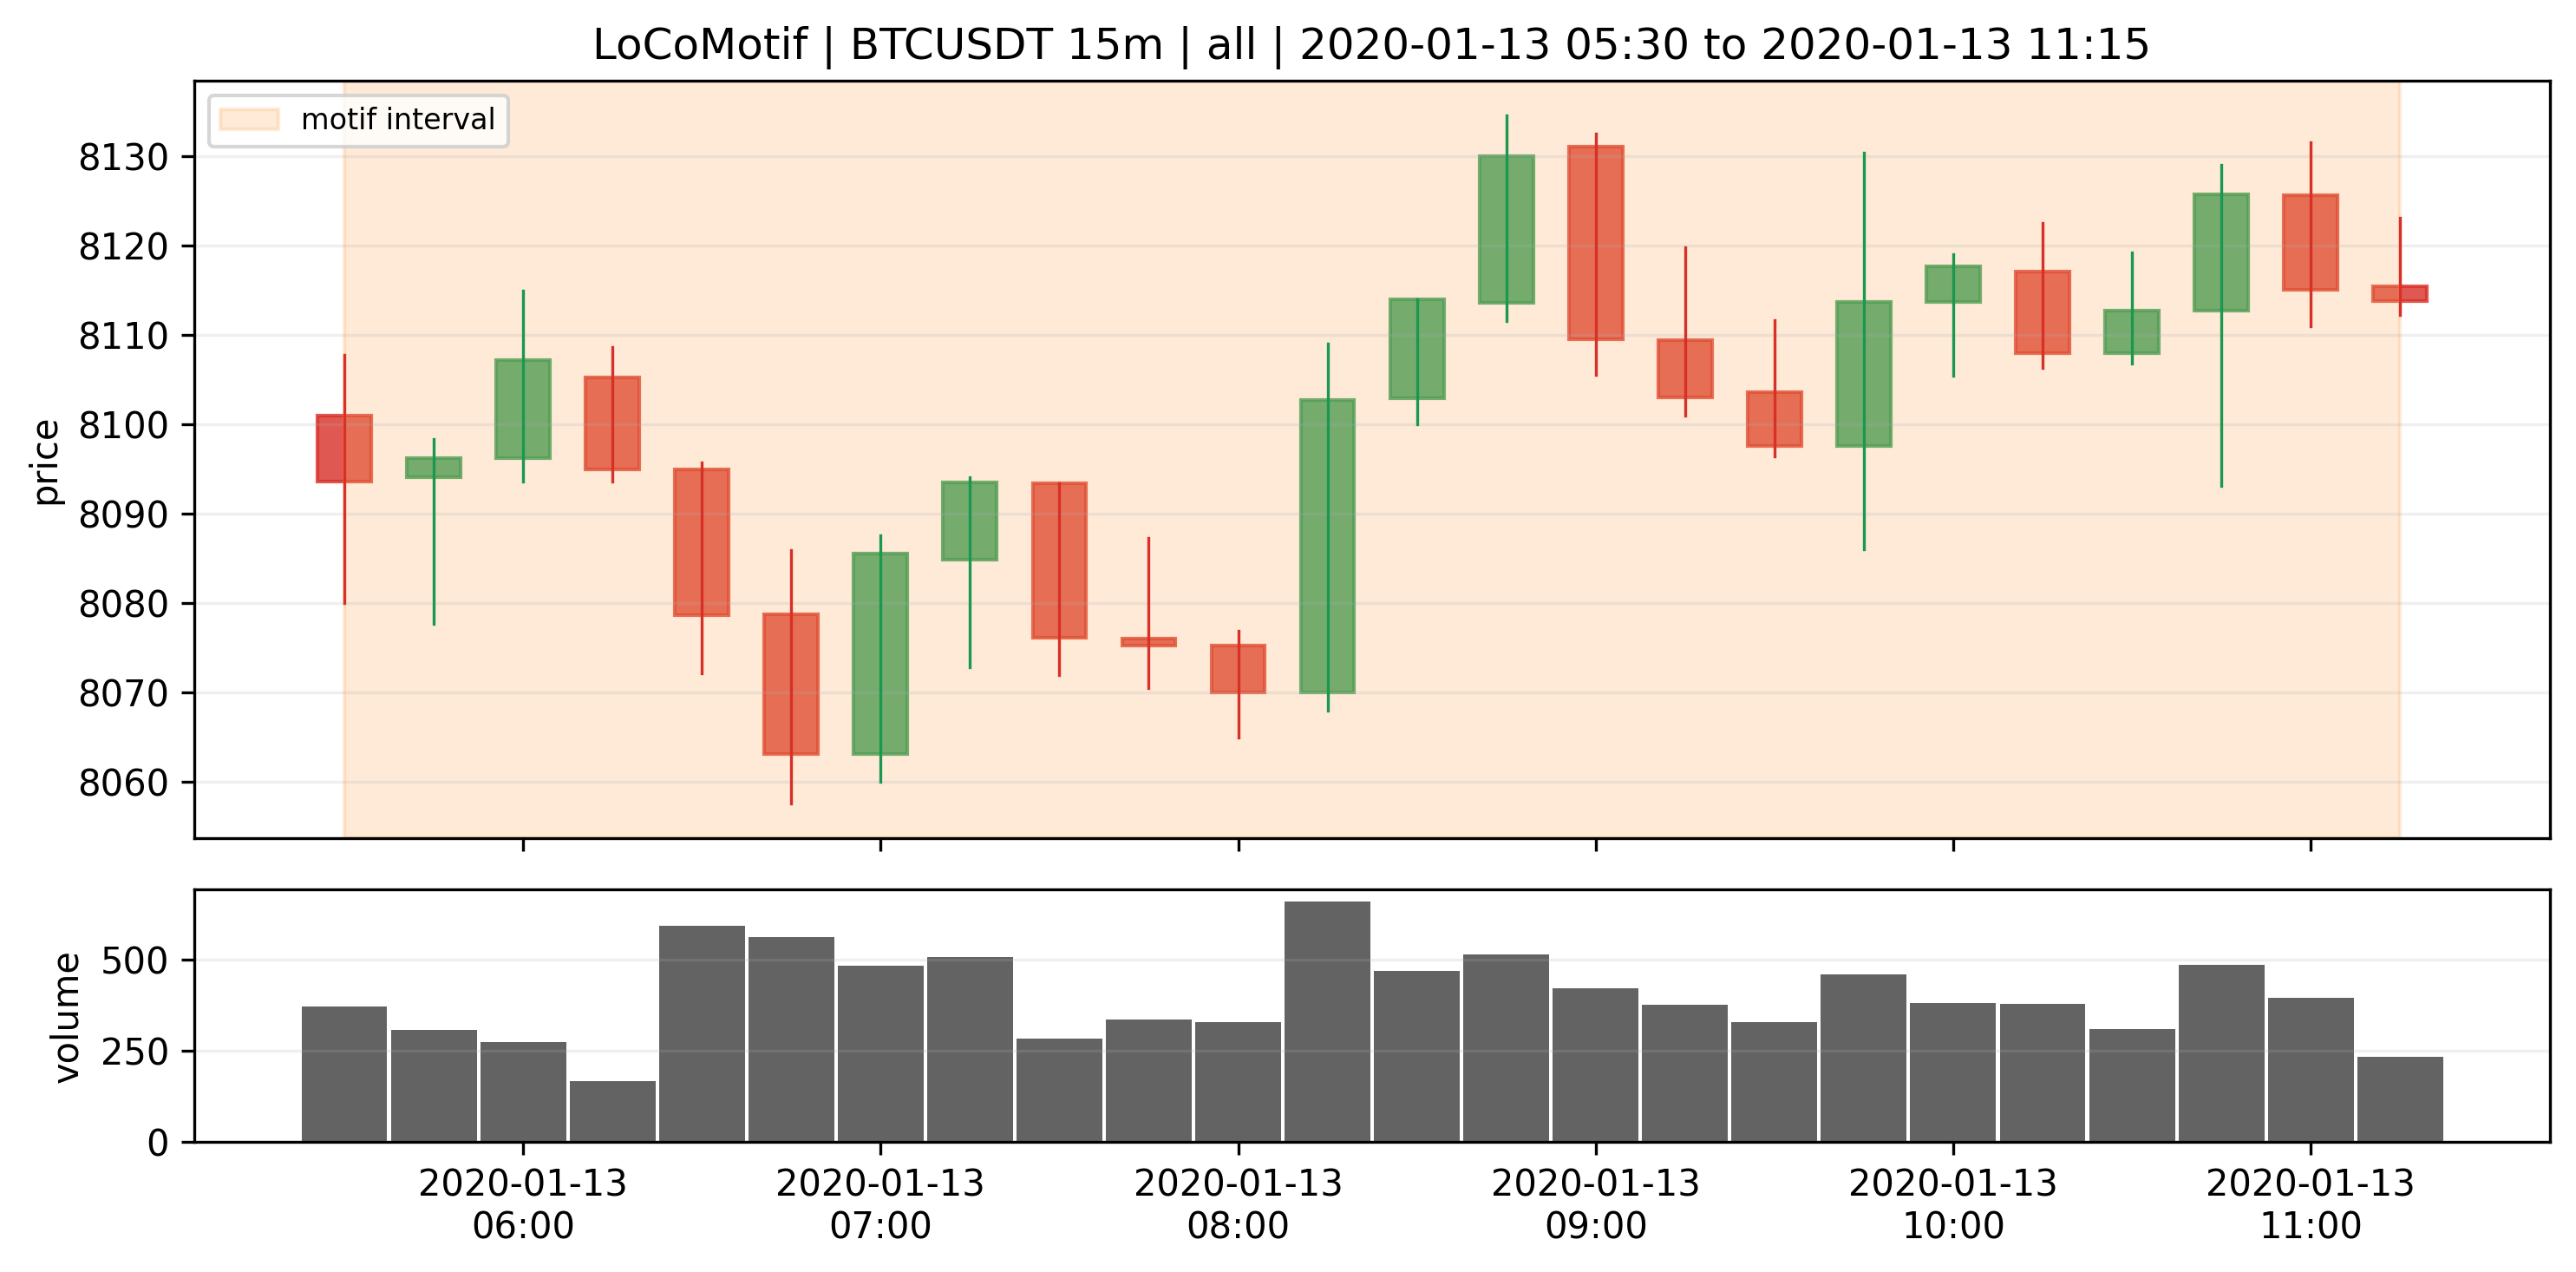
\includegraphics[width=0.9\linewidth]{reports/final_visual_evidence/figures/motif_01_locomotif_btcusdt_15m_all_1_0_1_0_zoom.png}
\caption{motif 01 locomotif btcusdt 15m all 1 0 1 0 zoom. The figure compares real available Matrix Profile and LoCoMotif outputs while preserving object-type differences.}
\end{figure}

\begin{figure}[ht]
\centering
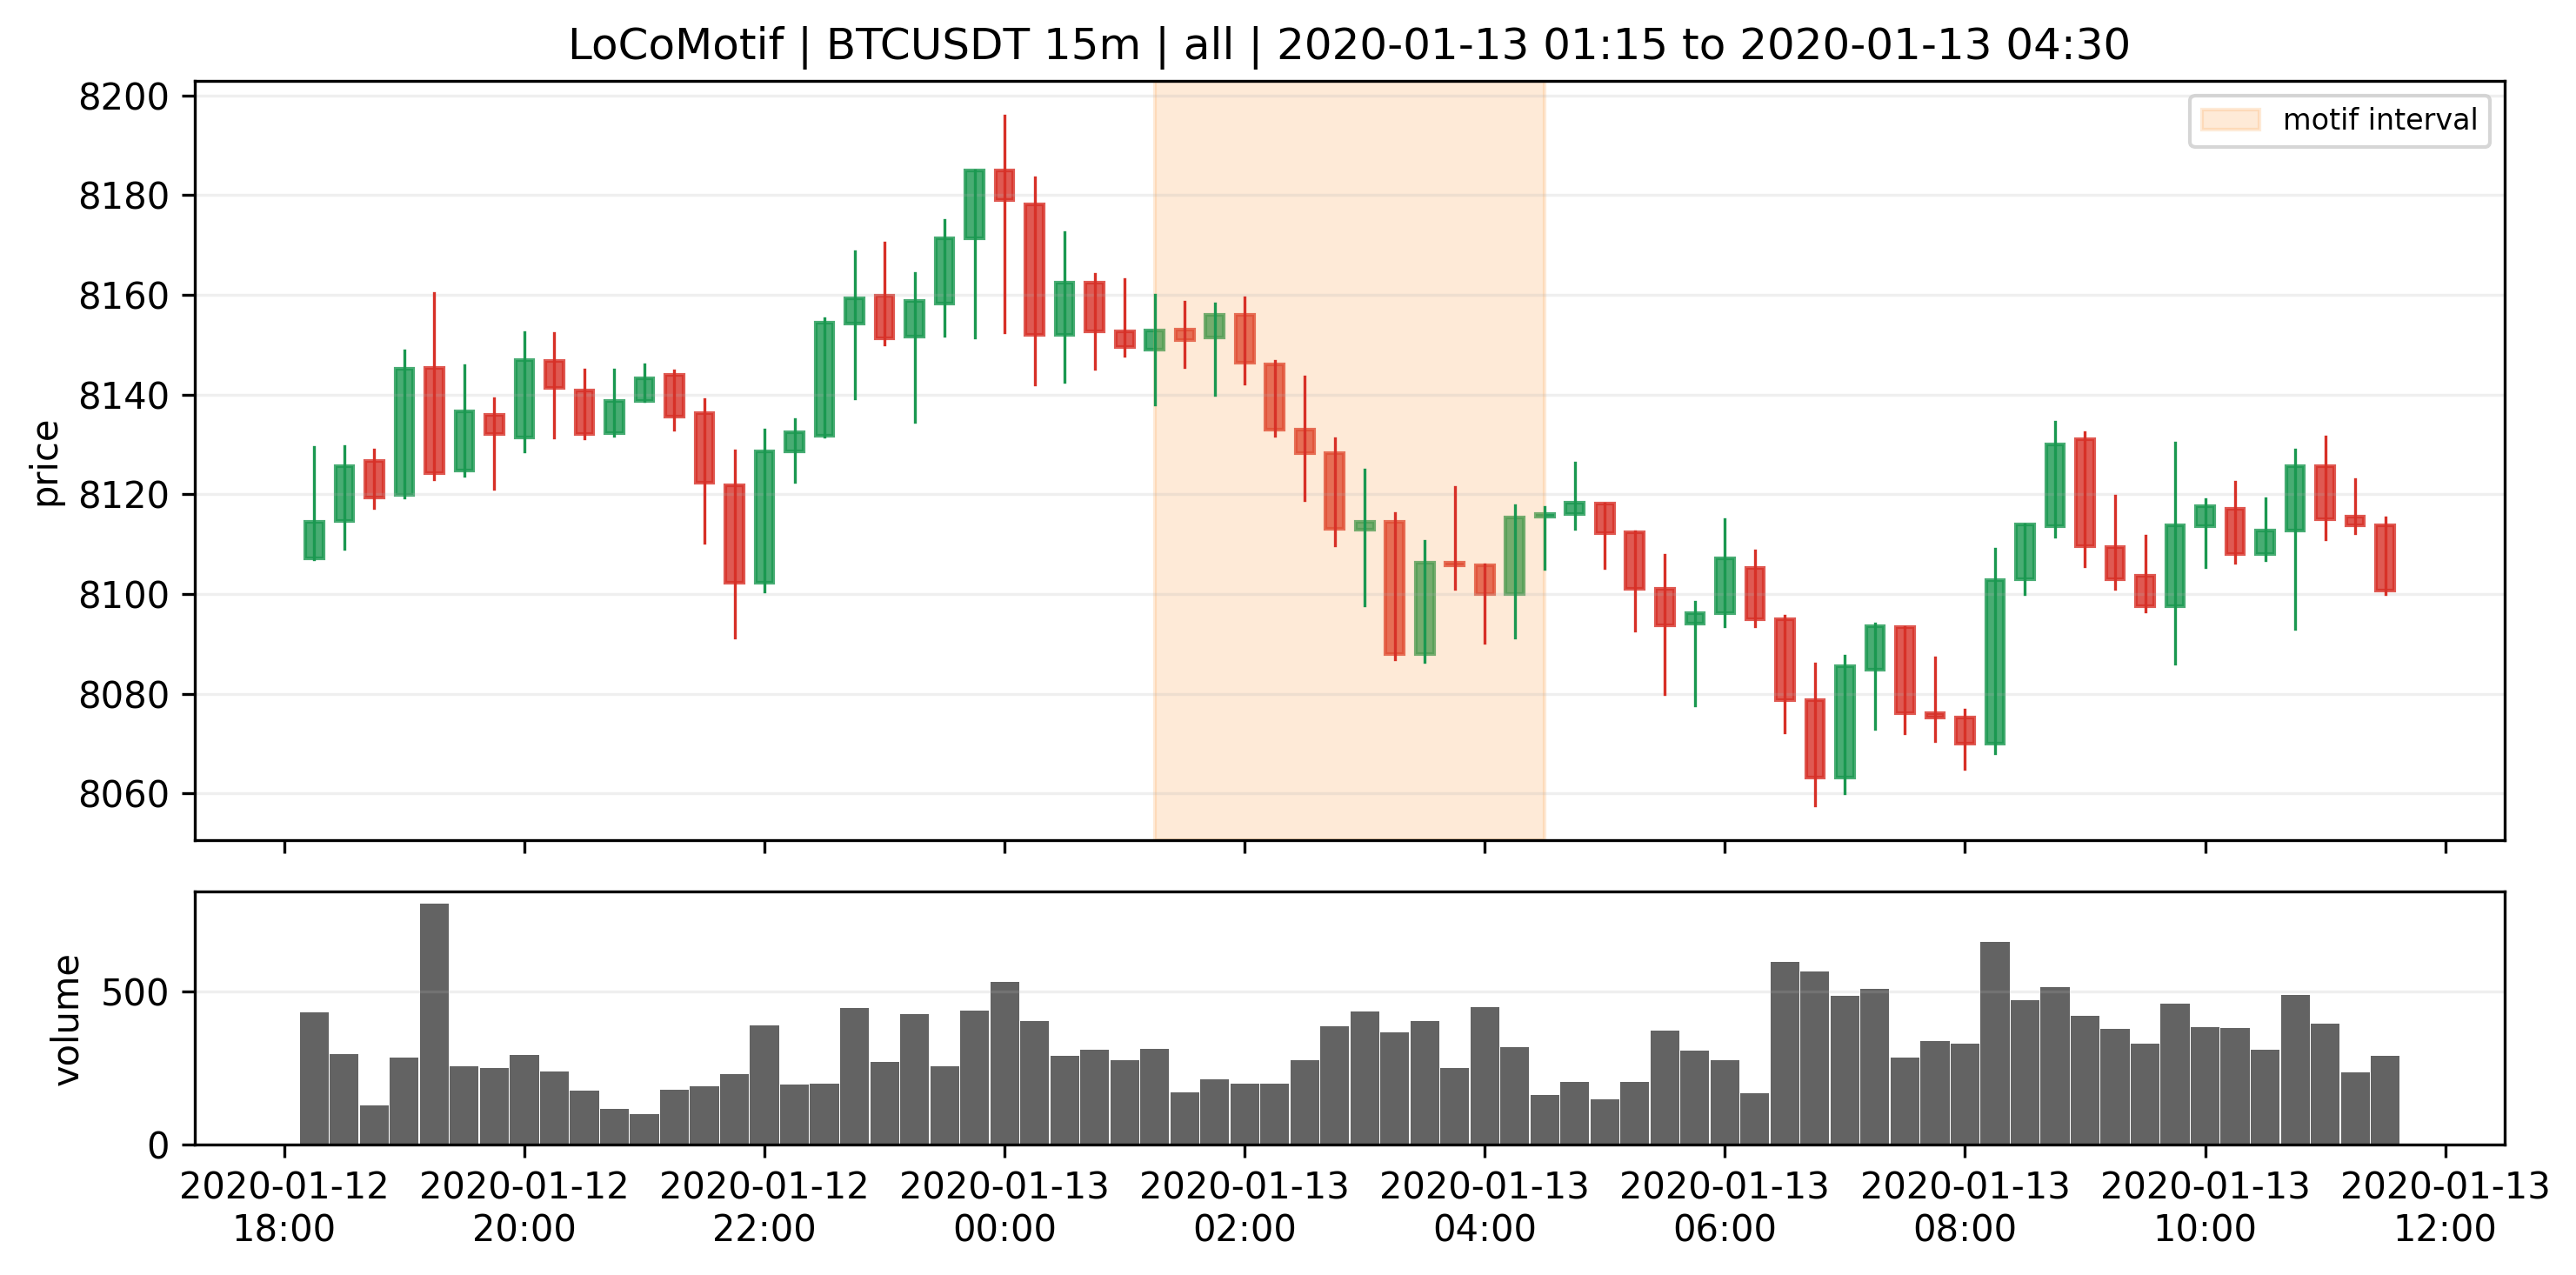
\includegraphics[width=0.9\linewidth]{reports/final_visual_evidence/figures/motif_02_locomotif_btcusdt_15m_all_1_0_3_0_context.png}
\caption{motif 02 locomotif btcusdt 15m all 1 0 3 0 context. The figure compares real available Matrix Profile and LoCoMotif outputs while preserving object-type differences.}
\end{figure}

\begin{figure}[ht]
\centering
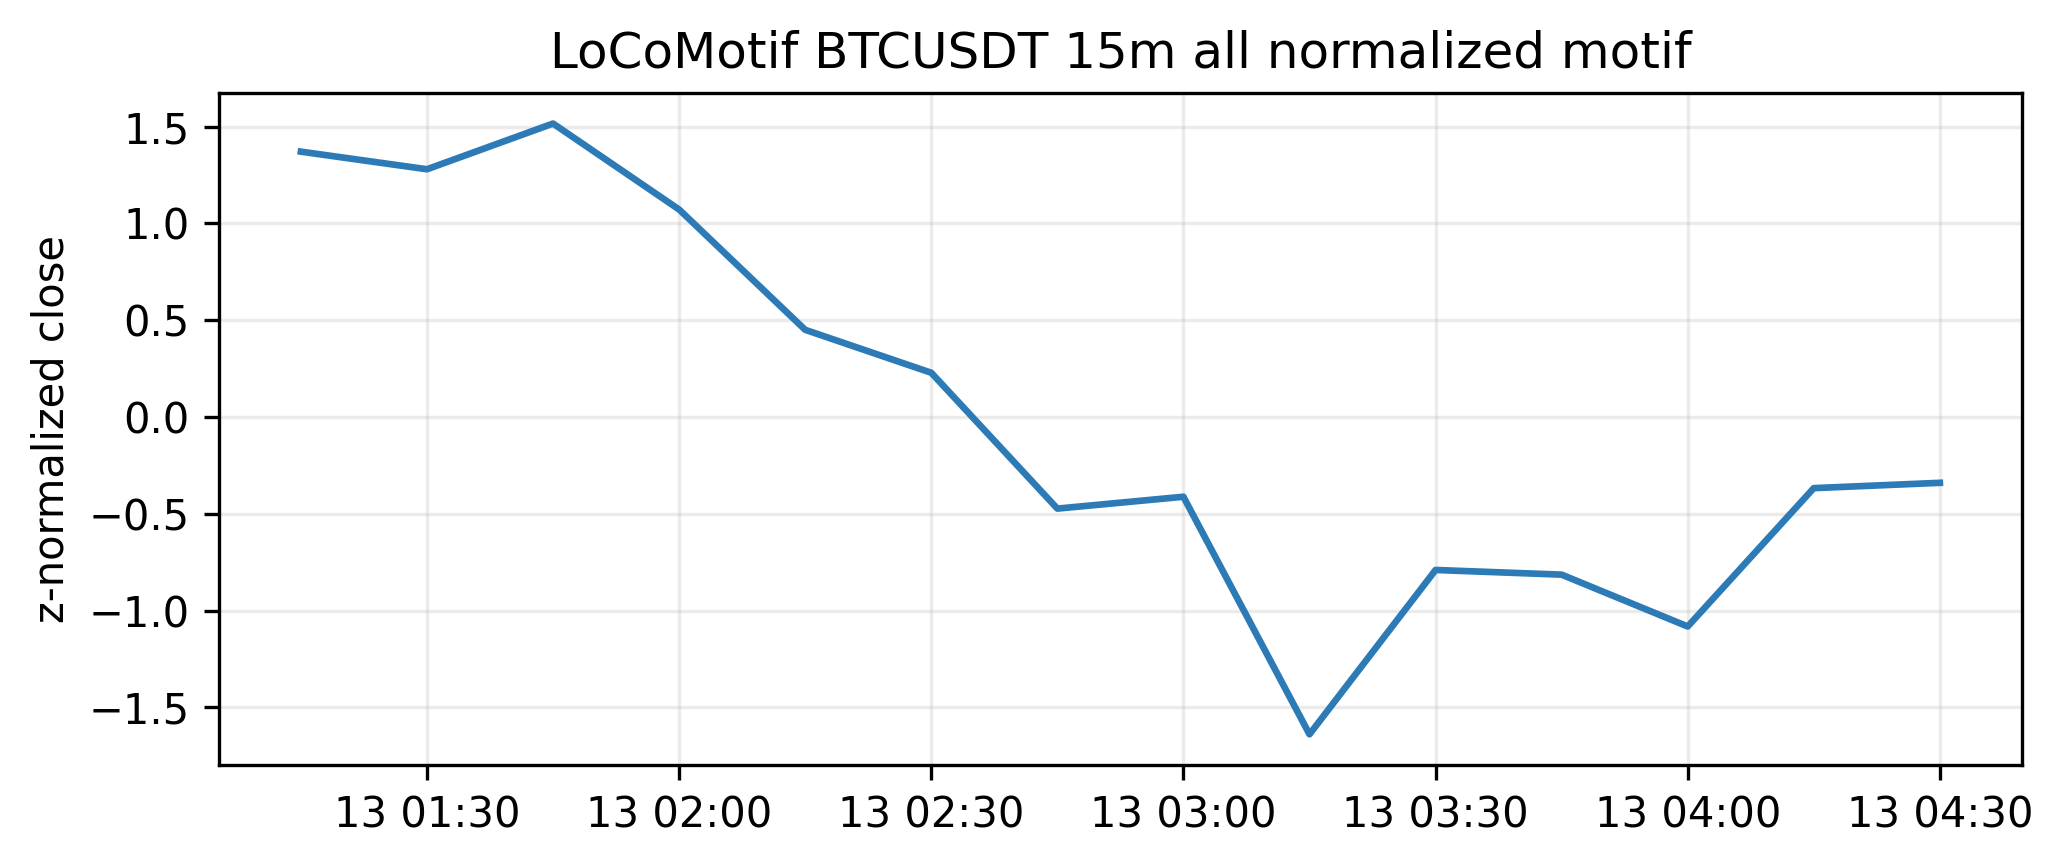
\includegraphics[width=0.9\linewidth]{reports/final_visual_evidence/figures/motif_02_locomotif_btcusdt_15m_all_1_0_3_0_normal_pattern.png}
\caption{motif 02 locomotif btcusdt 15m all 1 0 3 0 normal pattern. The figure compares real available Matrix Profile and LoCoMotif outputs while preserving object-type differences.}
\end{figure}

\begin{figure}[ht]
\centering
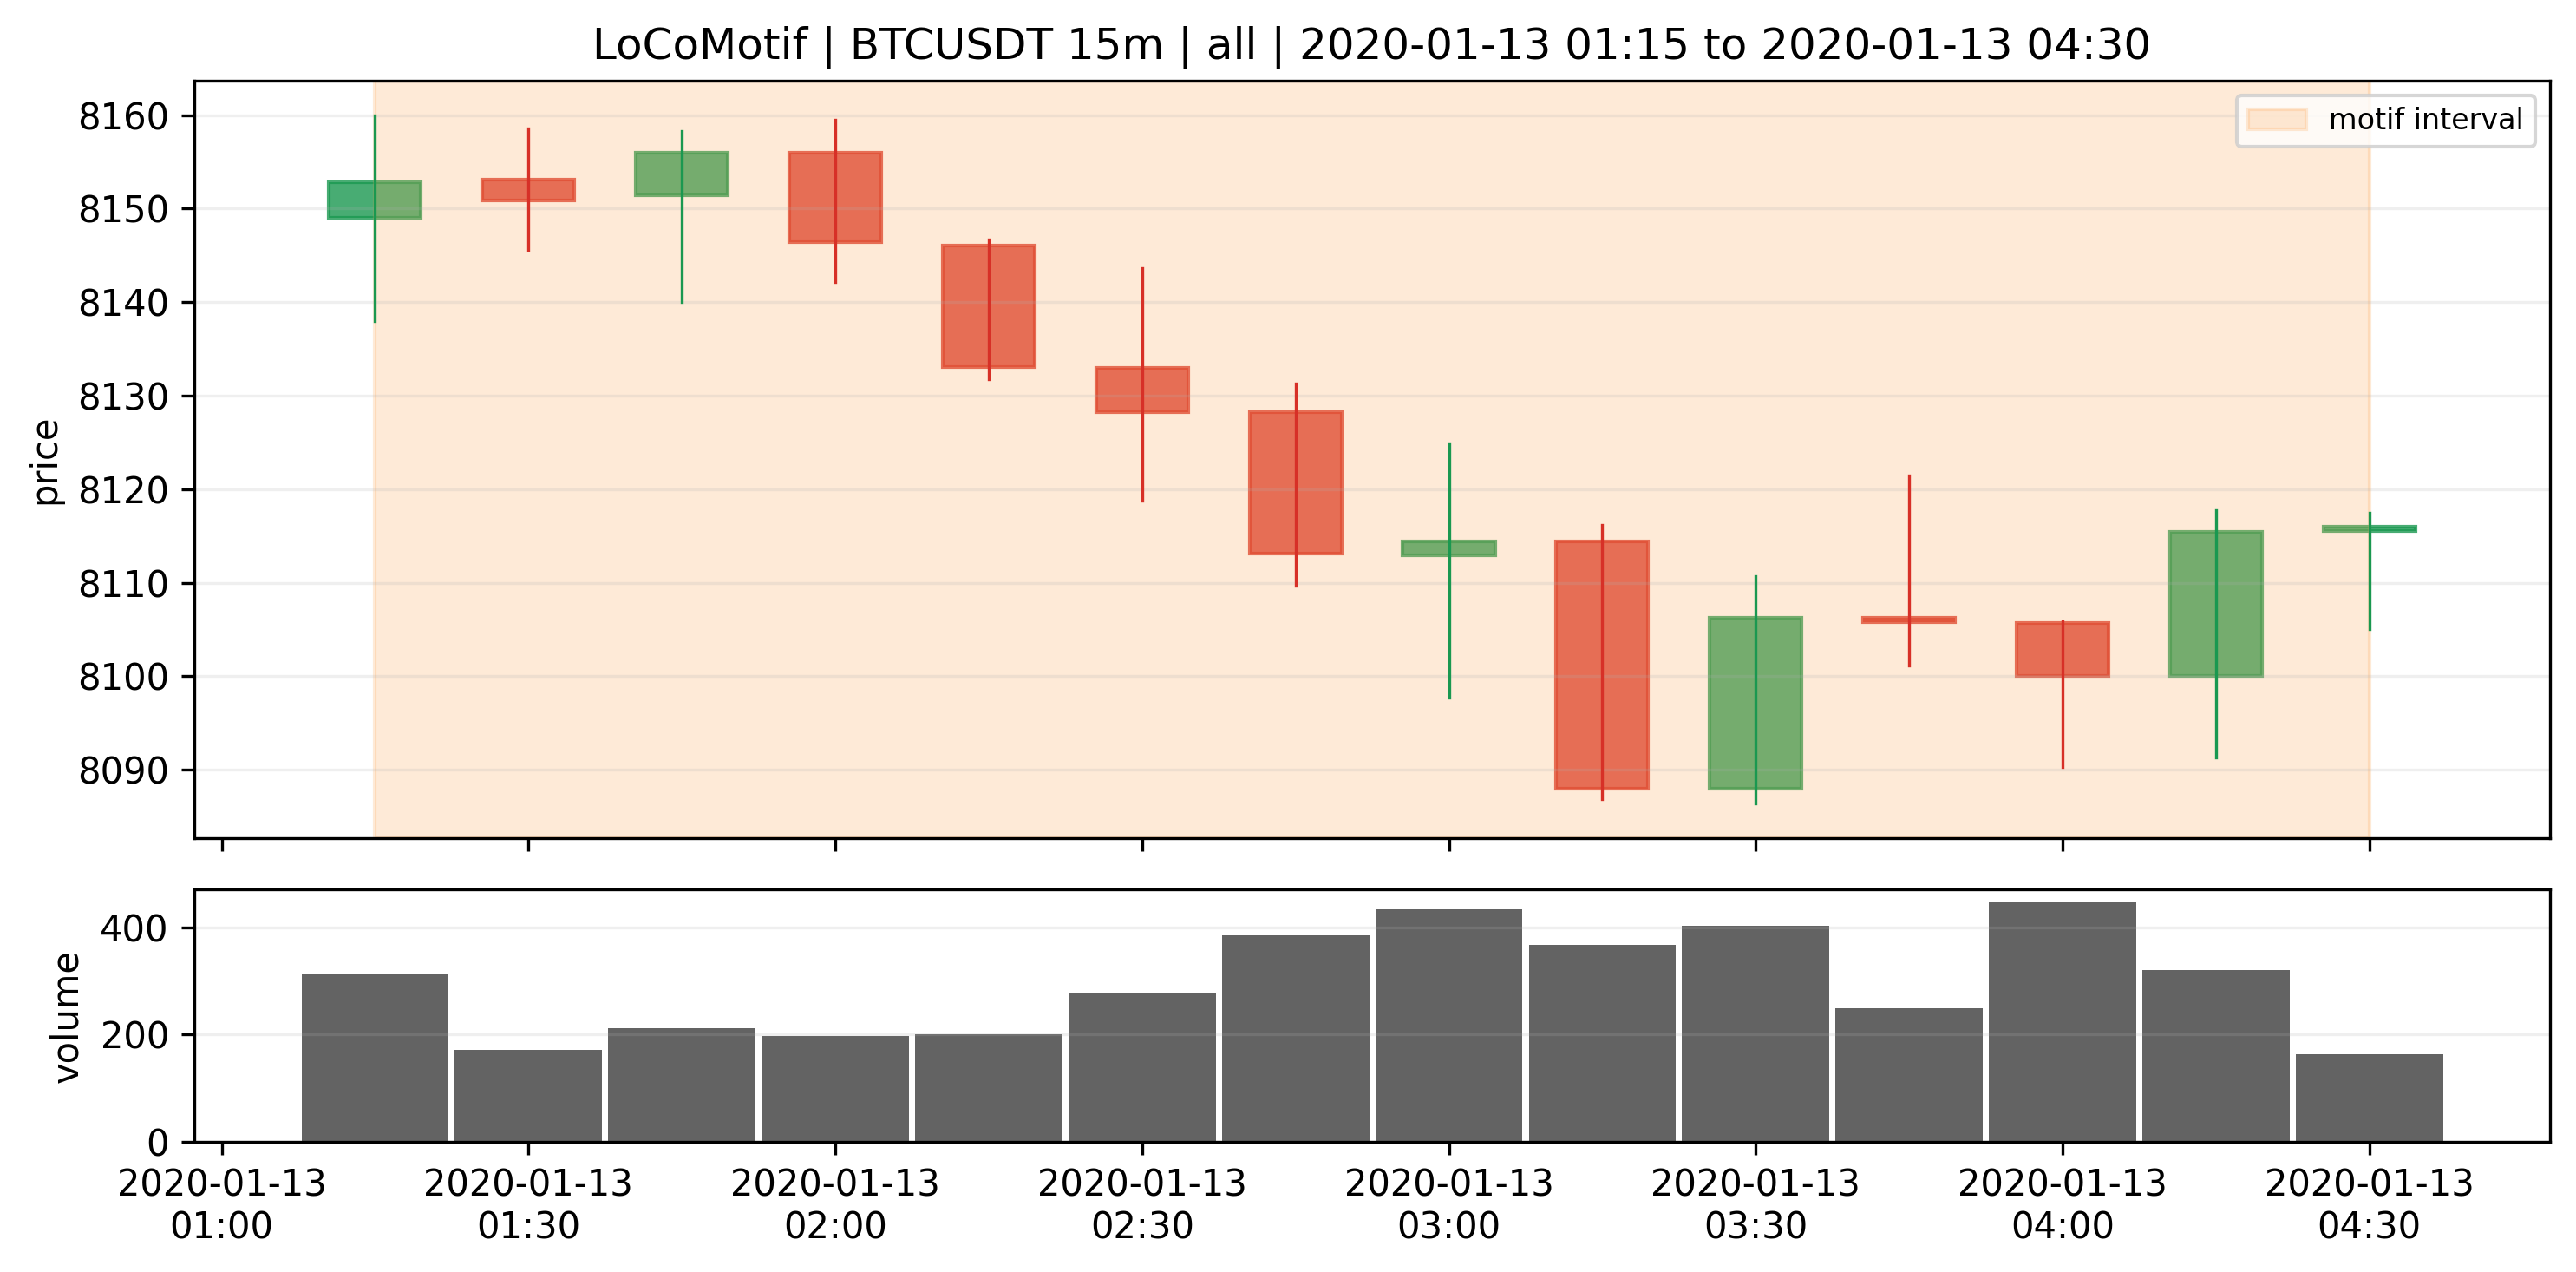
\includegraphics[width=0.9\linewidth]{reports/final_visual_evidence/figures/motif_02_locomotif_btcusdt_15m_all_1_0_3_0_zoom.png}
\caption{motif 02 locomotif btcusdt 15m all 1 0 3 0 zoom. The figure compares real available Matrix Profile and LoCoMotif outputs while preserving object-type differences.}
\end{figure}

\begin{figure}[ht]
\centering
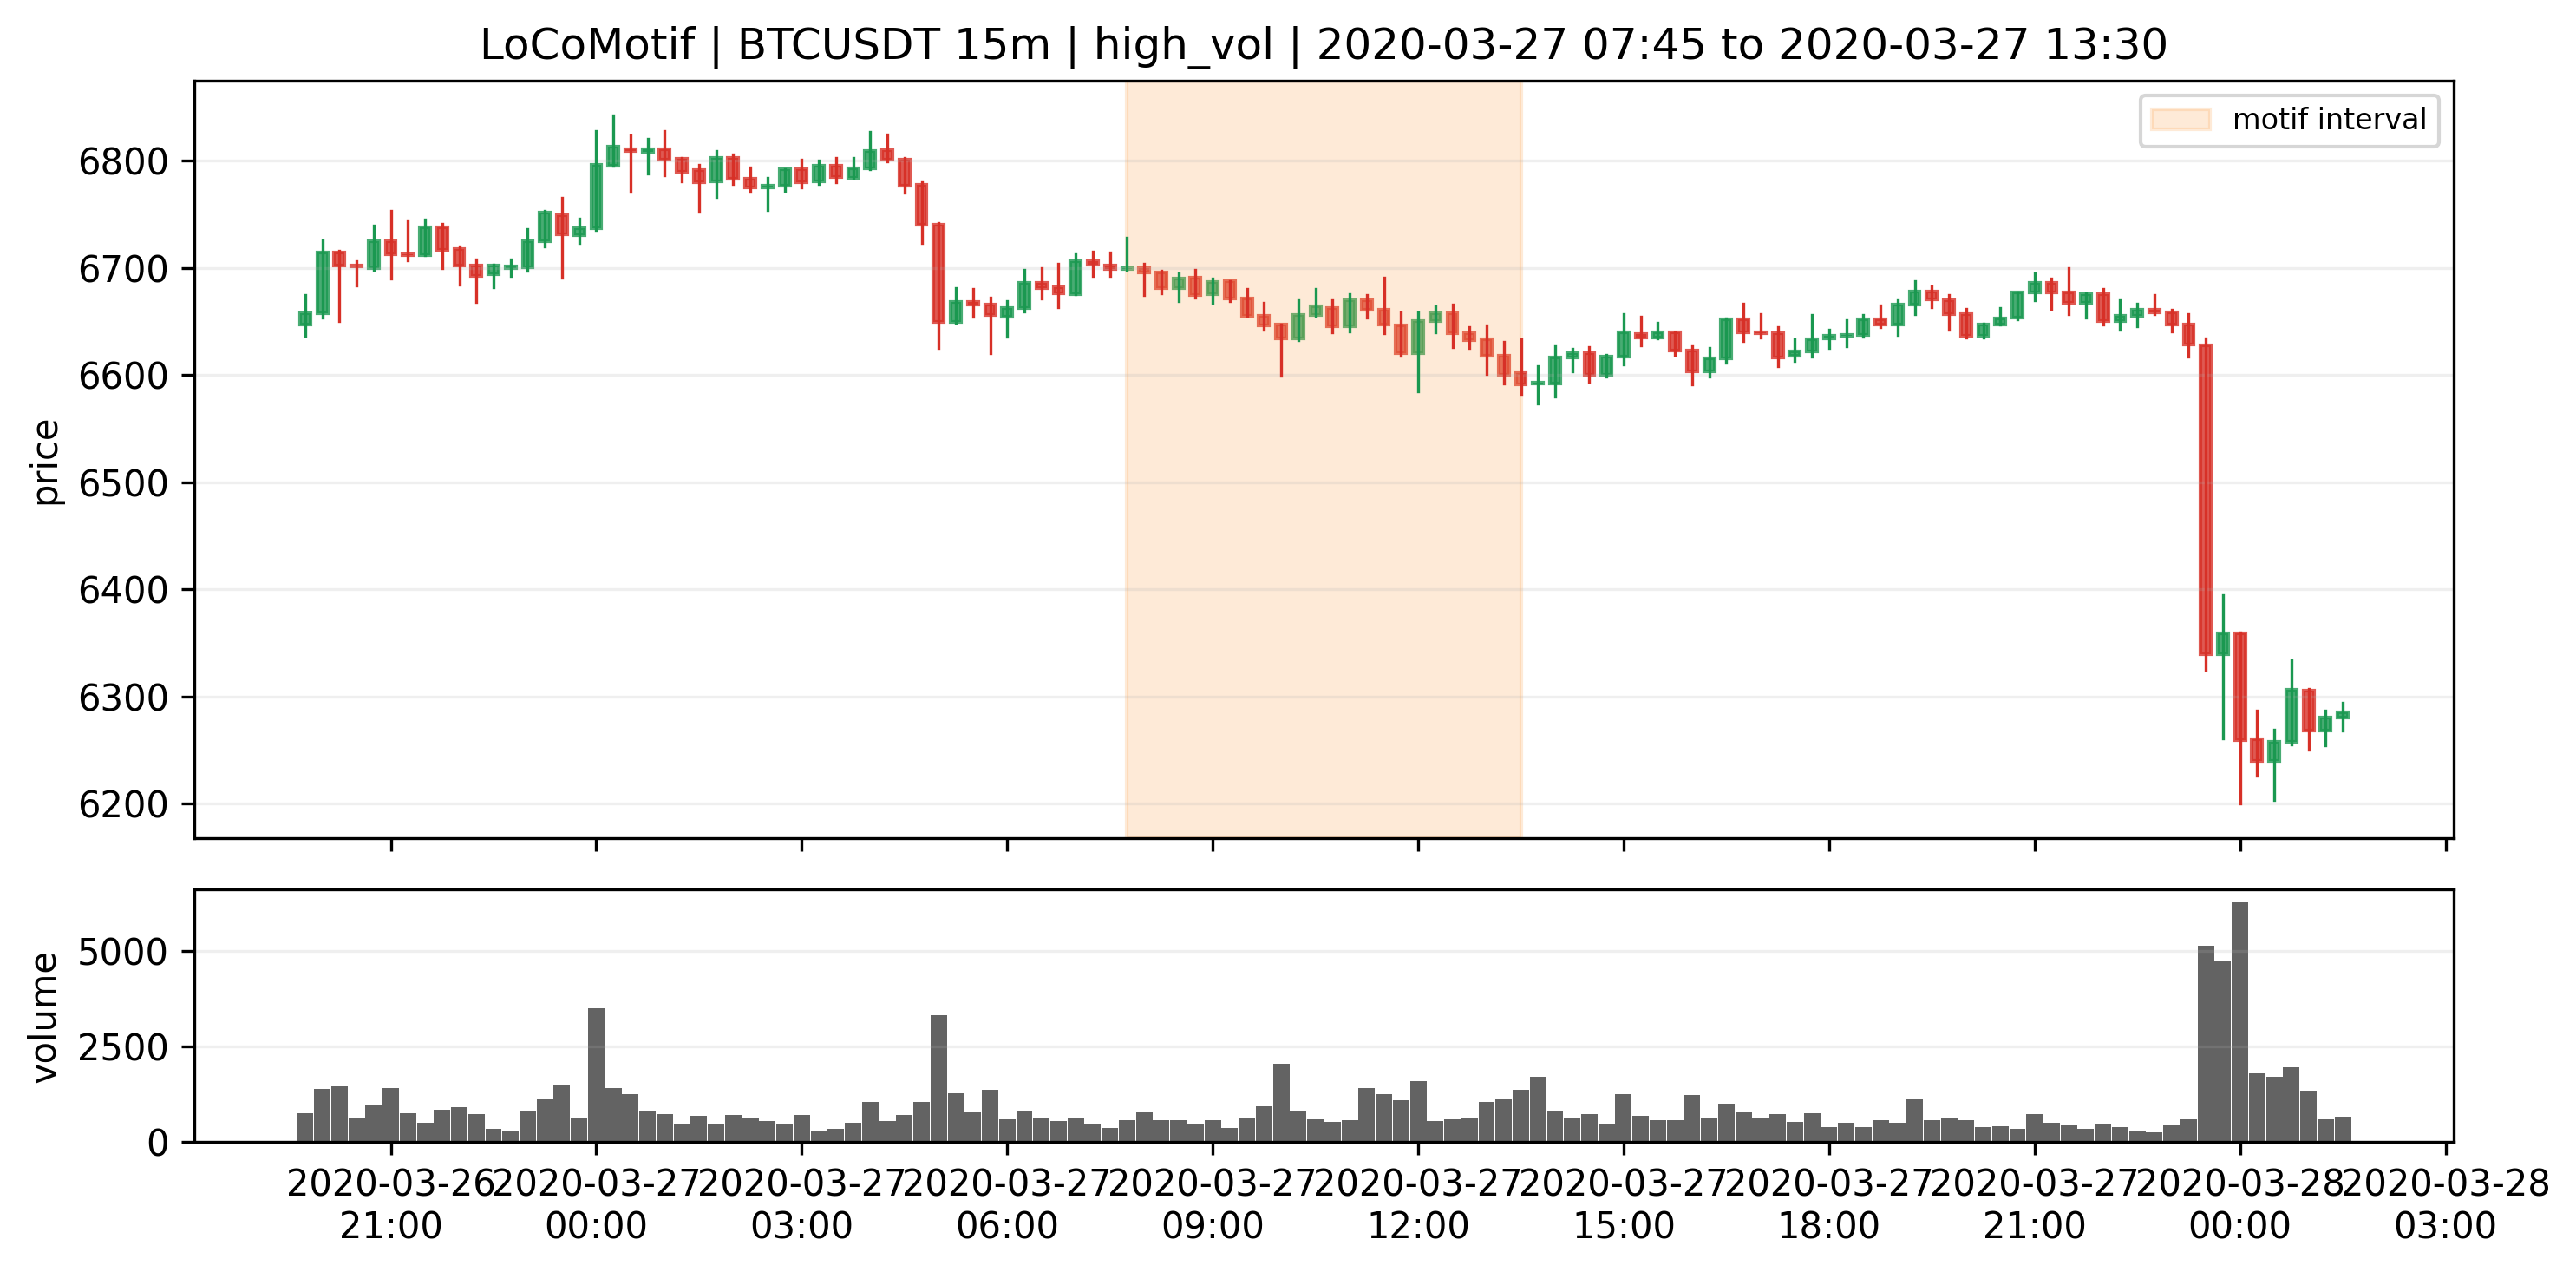
\includegraphics[width=0.9\linewidth]{reports/final_visual_evidence/figures/motif_03_locomotif_btcusdt_15m_high_vol_1_0_1_0_context.png}
\caption{motif 03 locomotif btcusdt 15m high vol 1 0 1 0 context. The figure compares real available Matrix Profile and LoCoMotif outputs while preserving object-type differences.}
\end{figure}

\begin{figure}[ht]
\centering
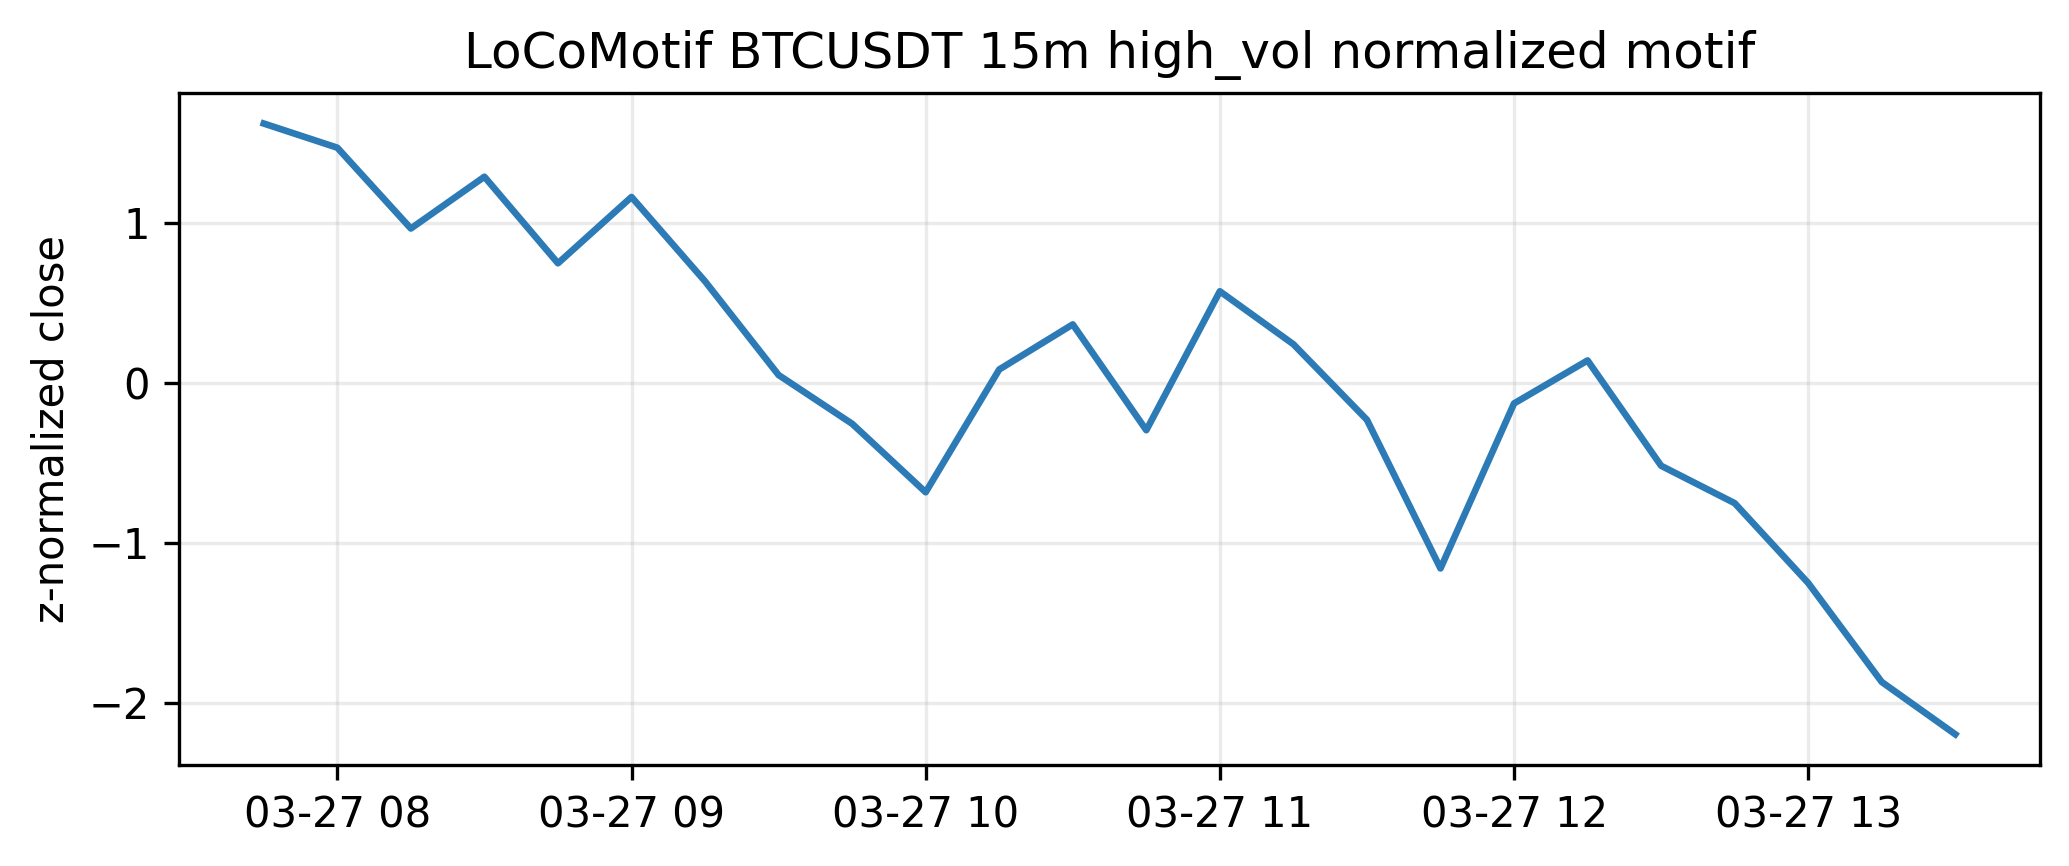
\includegraphics[width=0.9\linewidth]{reports/final_visual_evidence/figures/motif_03_locomotif_btcusdt_15m_high_vol_1_0_1_0_normal_pattern.png}
\caption{motif 03 locomotif btcusdt 15m high vol 1 0 1 0 normal pattern. The figure compares real available Matrix Profile and LoCoMotif outputs while preserving object-type differences.}
\end{figure}

\begin{figure}[ht]
\centering
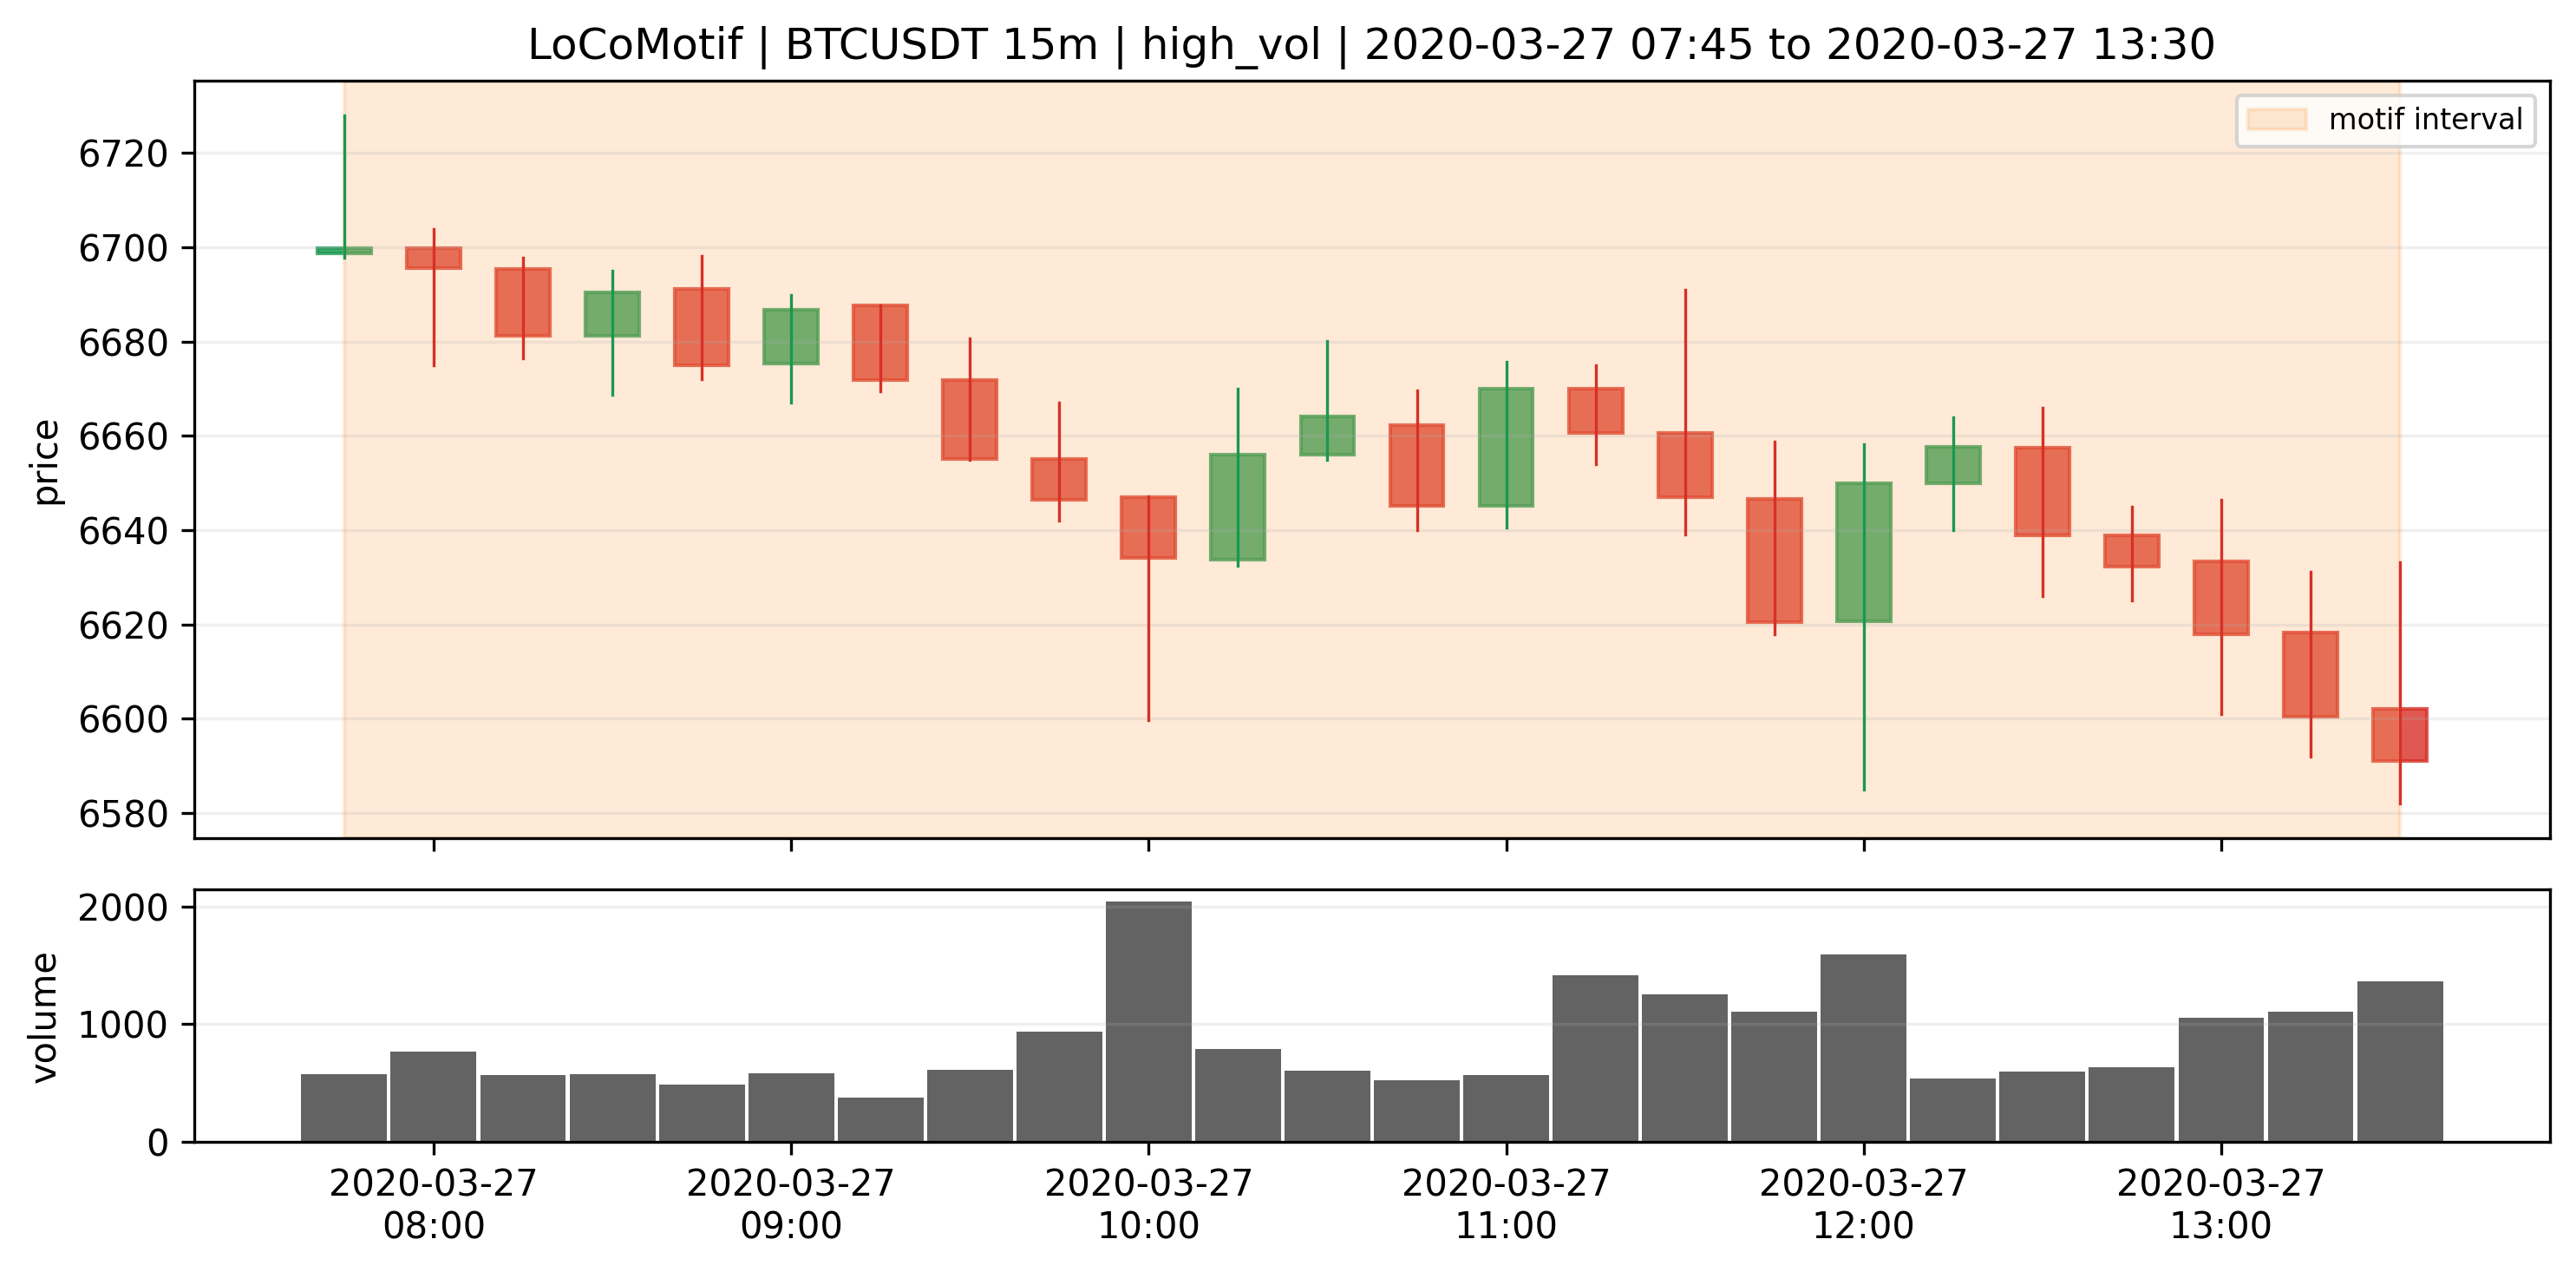
\includegraphics[width=0.9\linewidth]{reports/final_visual_evidence/figures/motif_03_locomotif_btcusdt_15m_high_vol_1_0_1_0_zoom.png}
\caption{motif 03 locomotif btcusdt 15m high vol 1 0 1 0 zoom. The figure compares real available Matrix Profile and LoCoMotif outputs while preserving object-type differences.}
\end{figure}

\begin{figure}[ht]
\centering
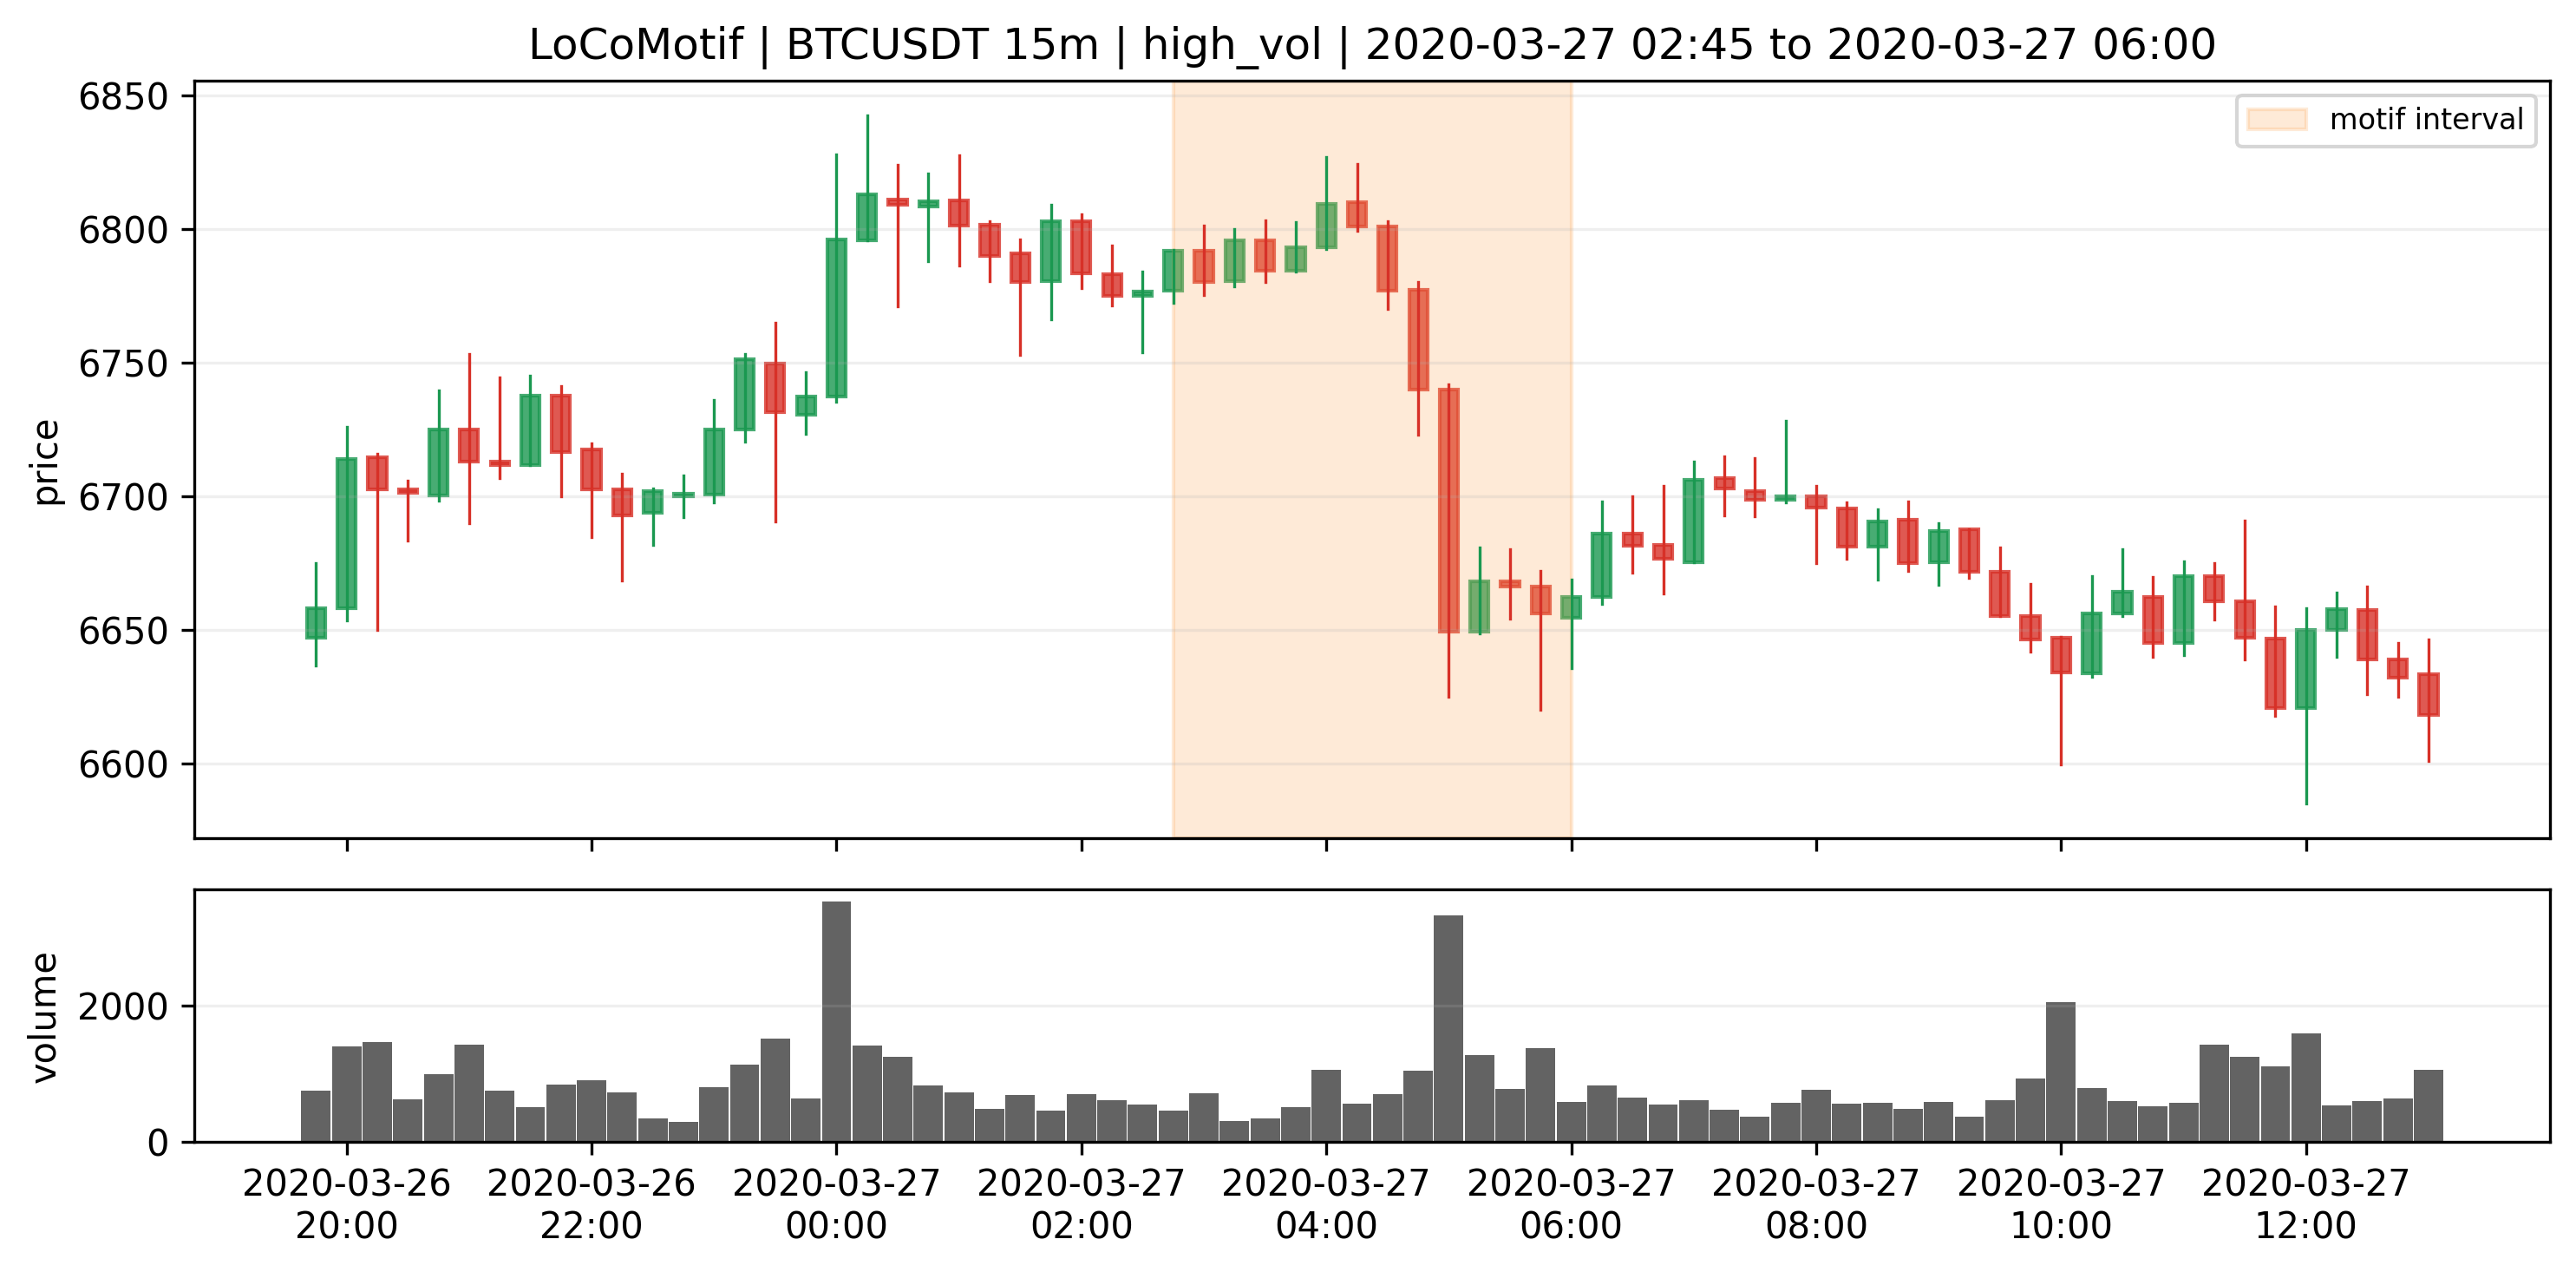
\includegraphics[width=0.9\linewidth]{reports/final_visual_evidence/figures/motif_04_locomotif_btcusdt_15m_high_vol_1_0_3_0_context.png}
\caption{motif 04 locomotif btcusdt 15m high vol 1 0 3 0 context. The figure compares real available Matrix Profile and LoCoMotif outputs while preserving object-type differences.}
\end{figure}

\begin{figure}[ht]
\centering
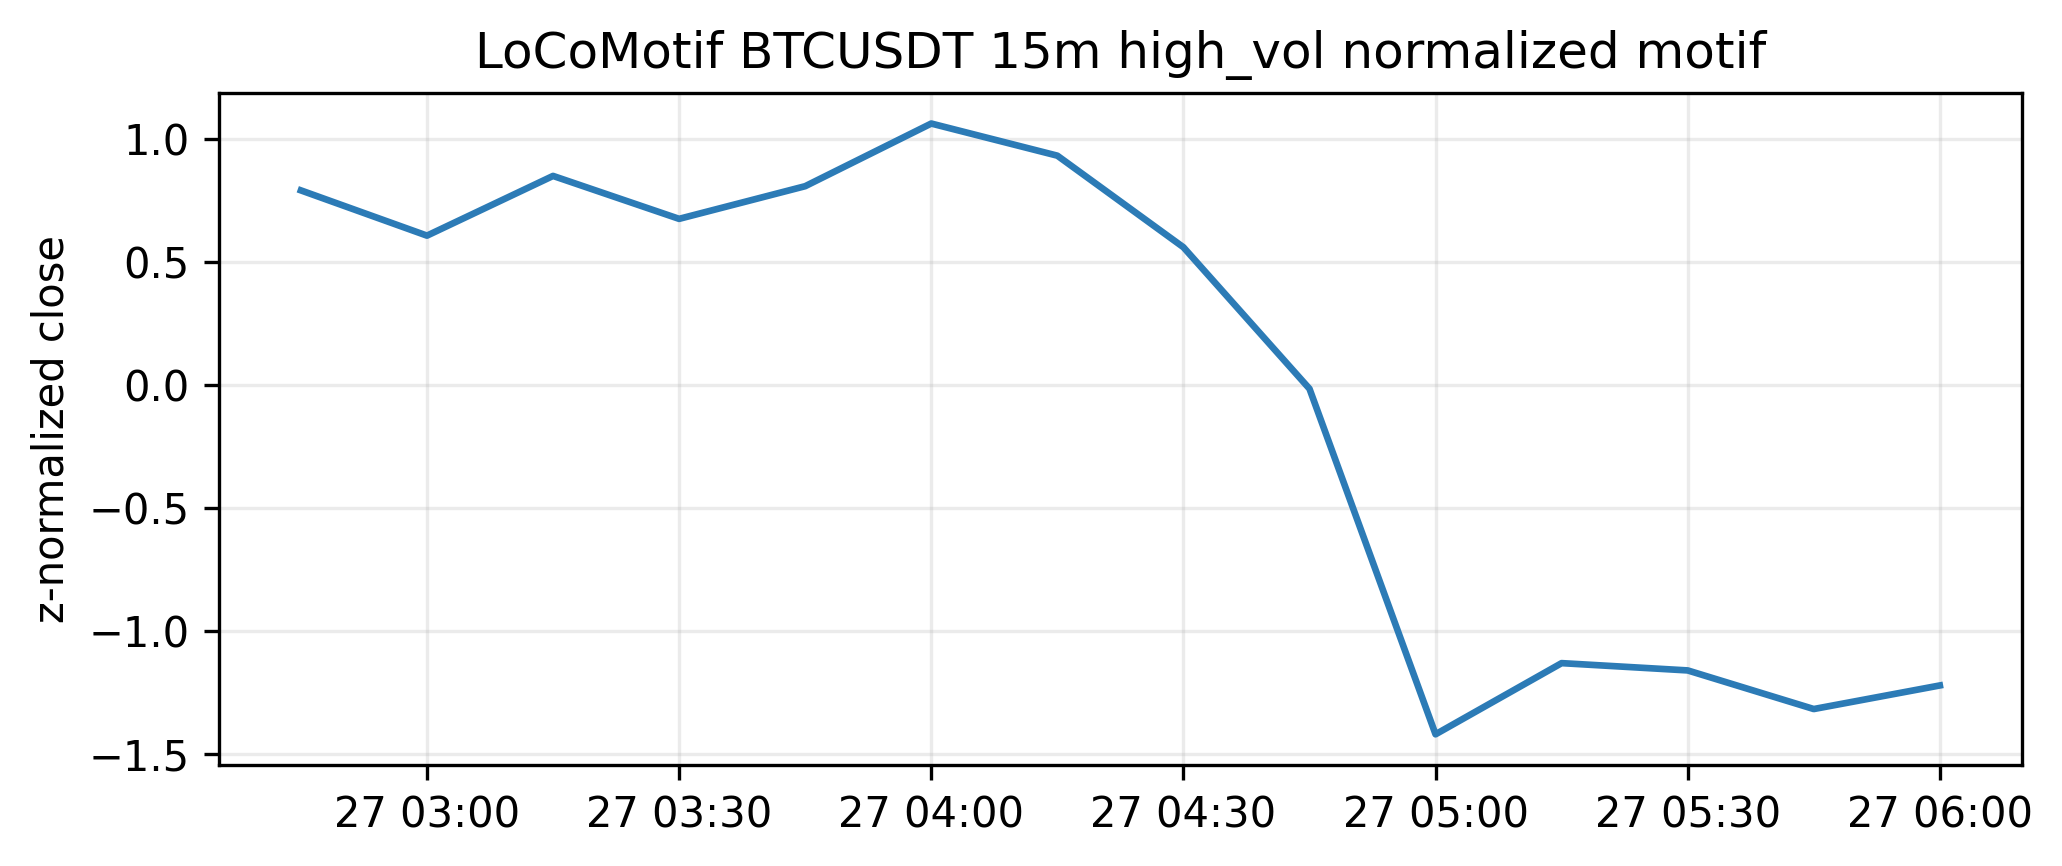
\includegraphics[width=0.9\linewidth]{reports/final_visual_evidence/figures/motif_04_locomotif_btcusdt_15m_high_vol_1_0_3_0_normal_pattern.png}
\caption{motif 04 locomotif btcusdt 15m high vol 1 0 3 0 normal pattern. The figure compares real available Matrix Profile and LoCoMotif outputs while preserving object-type differences.}
\end{figure}

\begin{figure}[ht]
\centering
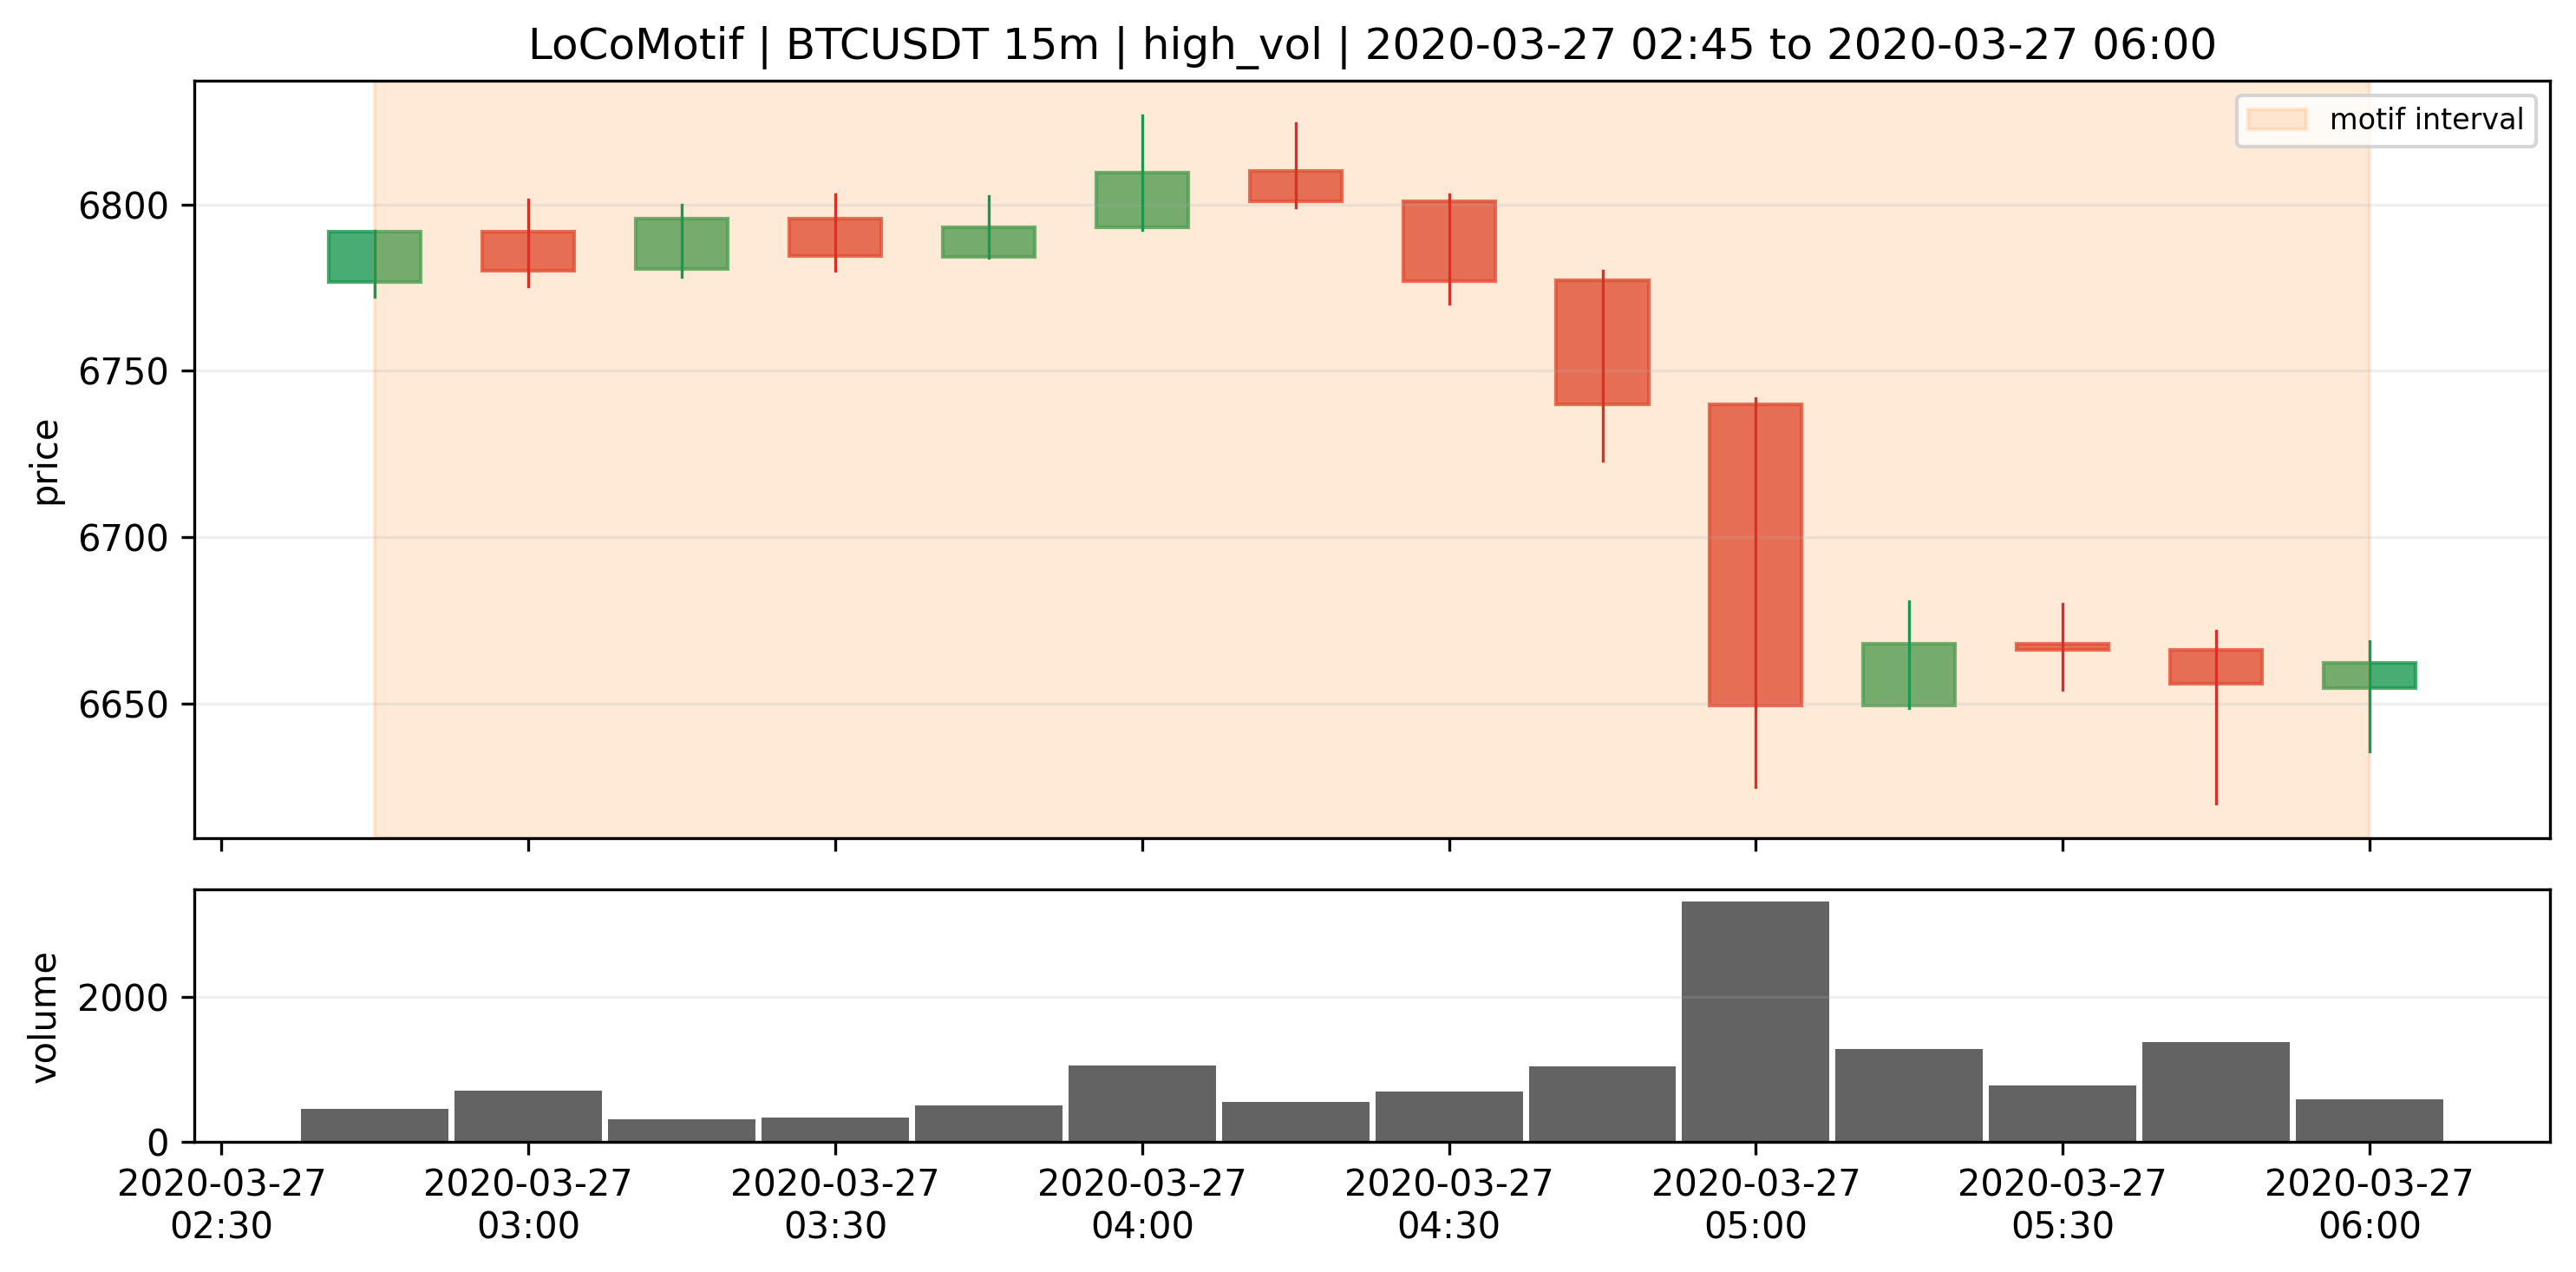
\includegraphics[width=0.9\linewidth]{reports/final_visual_evidence/figures/motif_04_locomotif_btcusdt_15m_high_vol_1_0_3_0_zoom.png}
\caption{motif 04 locomotif btcusdt 15m high vol 1 0 3 0 zoom. The figure compares real available Matrix Profile and LoCoMotif outputs while preserving object-type differences.}
\end{figure}

\begin{figure}[ht]
\centering
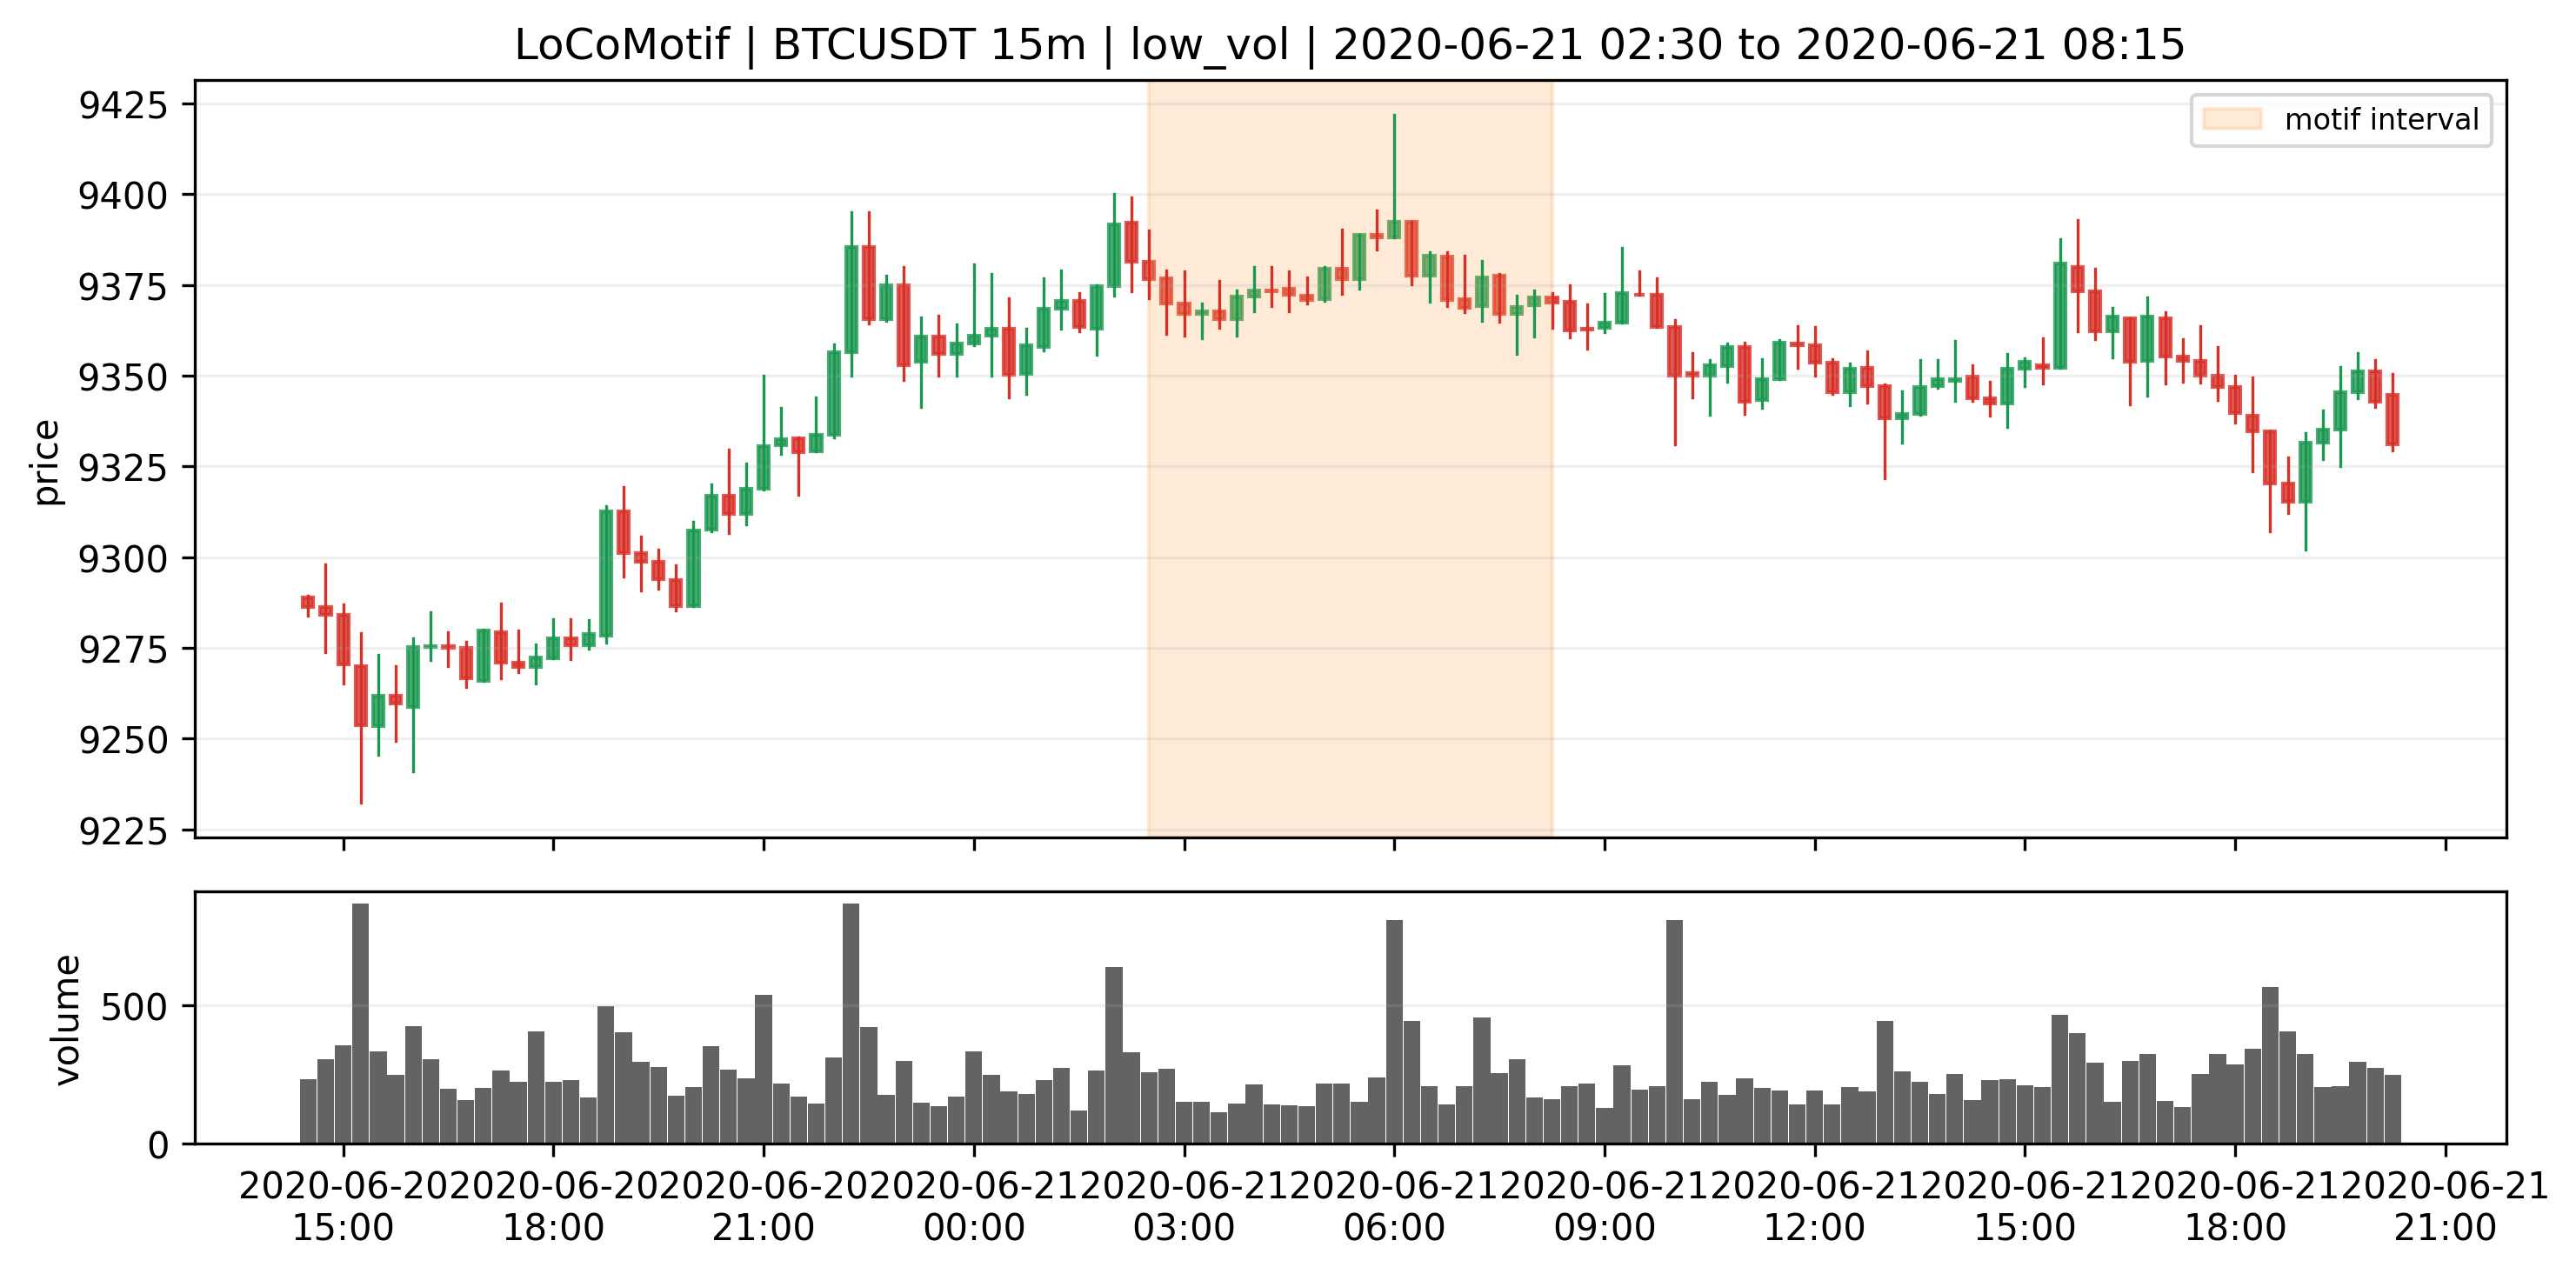
\includegraphics[width=0.9\linewidth]{reports/final_visual_evidence/figures/motif_05_locomotif_btcusdt_15m_low_vol_1_0_1_0_context.png}
\caption{motif 05 locomotif btcusdt 15m low vol 1 0 1 0 context. The figure compares real available Matrix Profile and LoCoMotif outputs while preserving object-type differences.}
\end{figure}

\begin{figure}[ht]
\centering
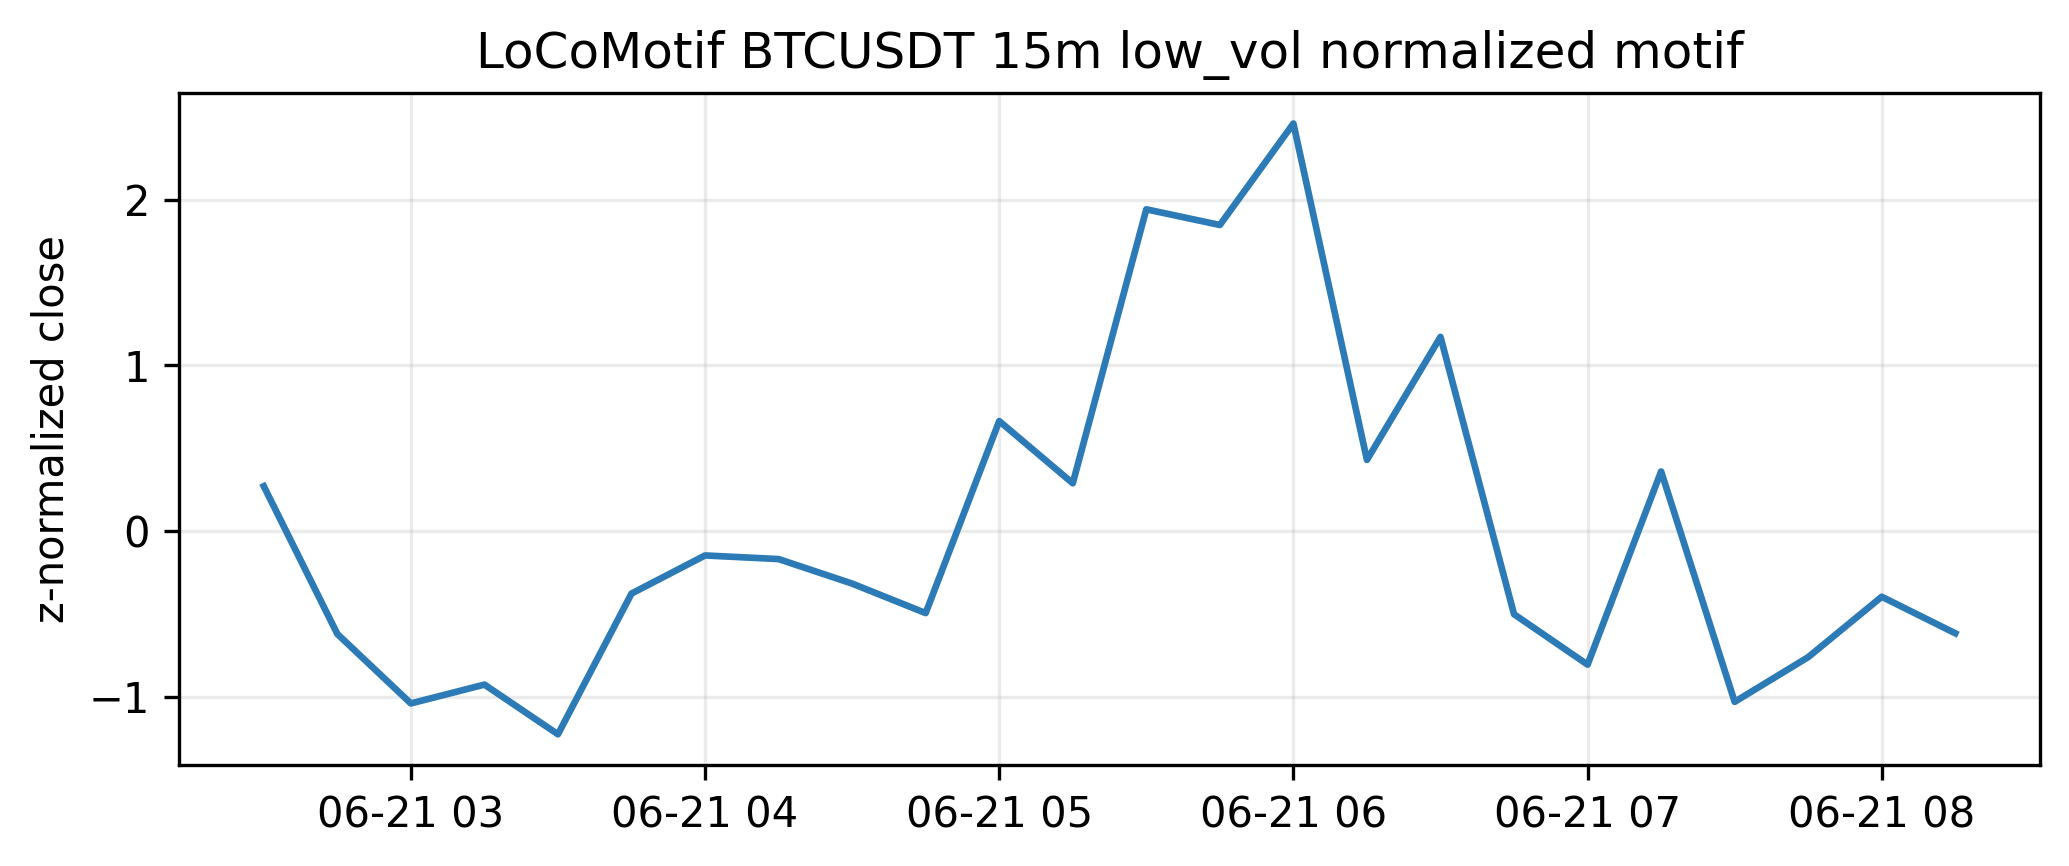
\includegraphics[width=0.9\linewidth]{reports/final_visual_evidence/figures/motif_05_locomotif_btcusdt_15m_low_vol_1_0_1_0_normal_pattern.png}
\caption{motif 05 locomotif btcusdt 15m low vol 1 0 1 0 normal pattern. The figure compares real available Matrix Profile and LoCoMotif outputs while preserving object-type differences.}
\end{figure}

\begin{figure}[ht]
\centering
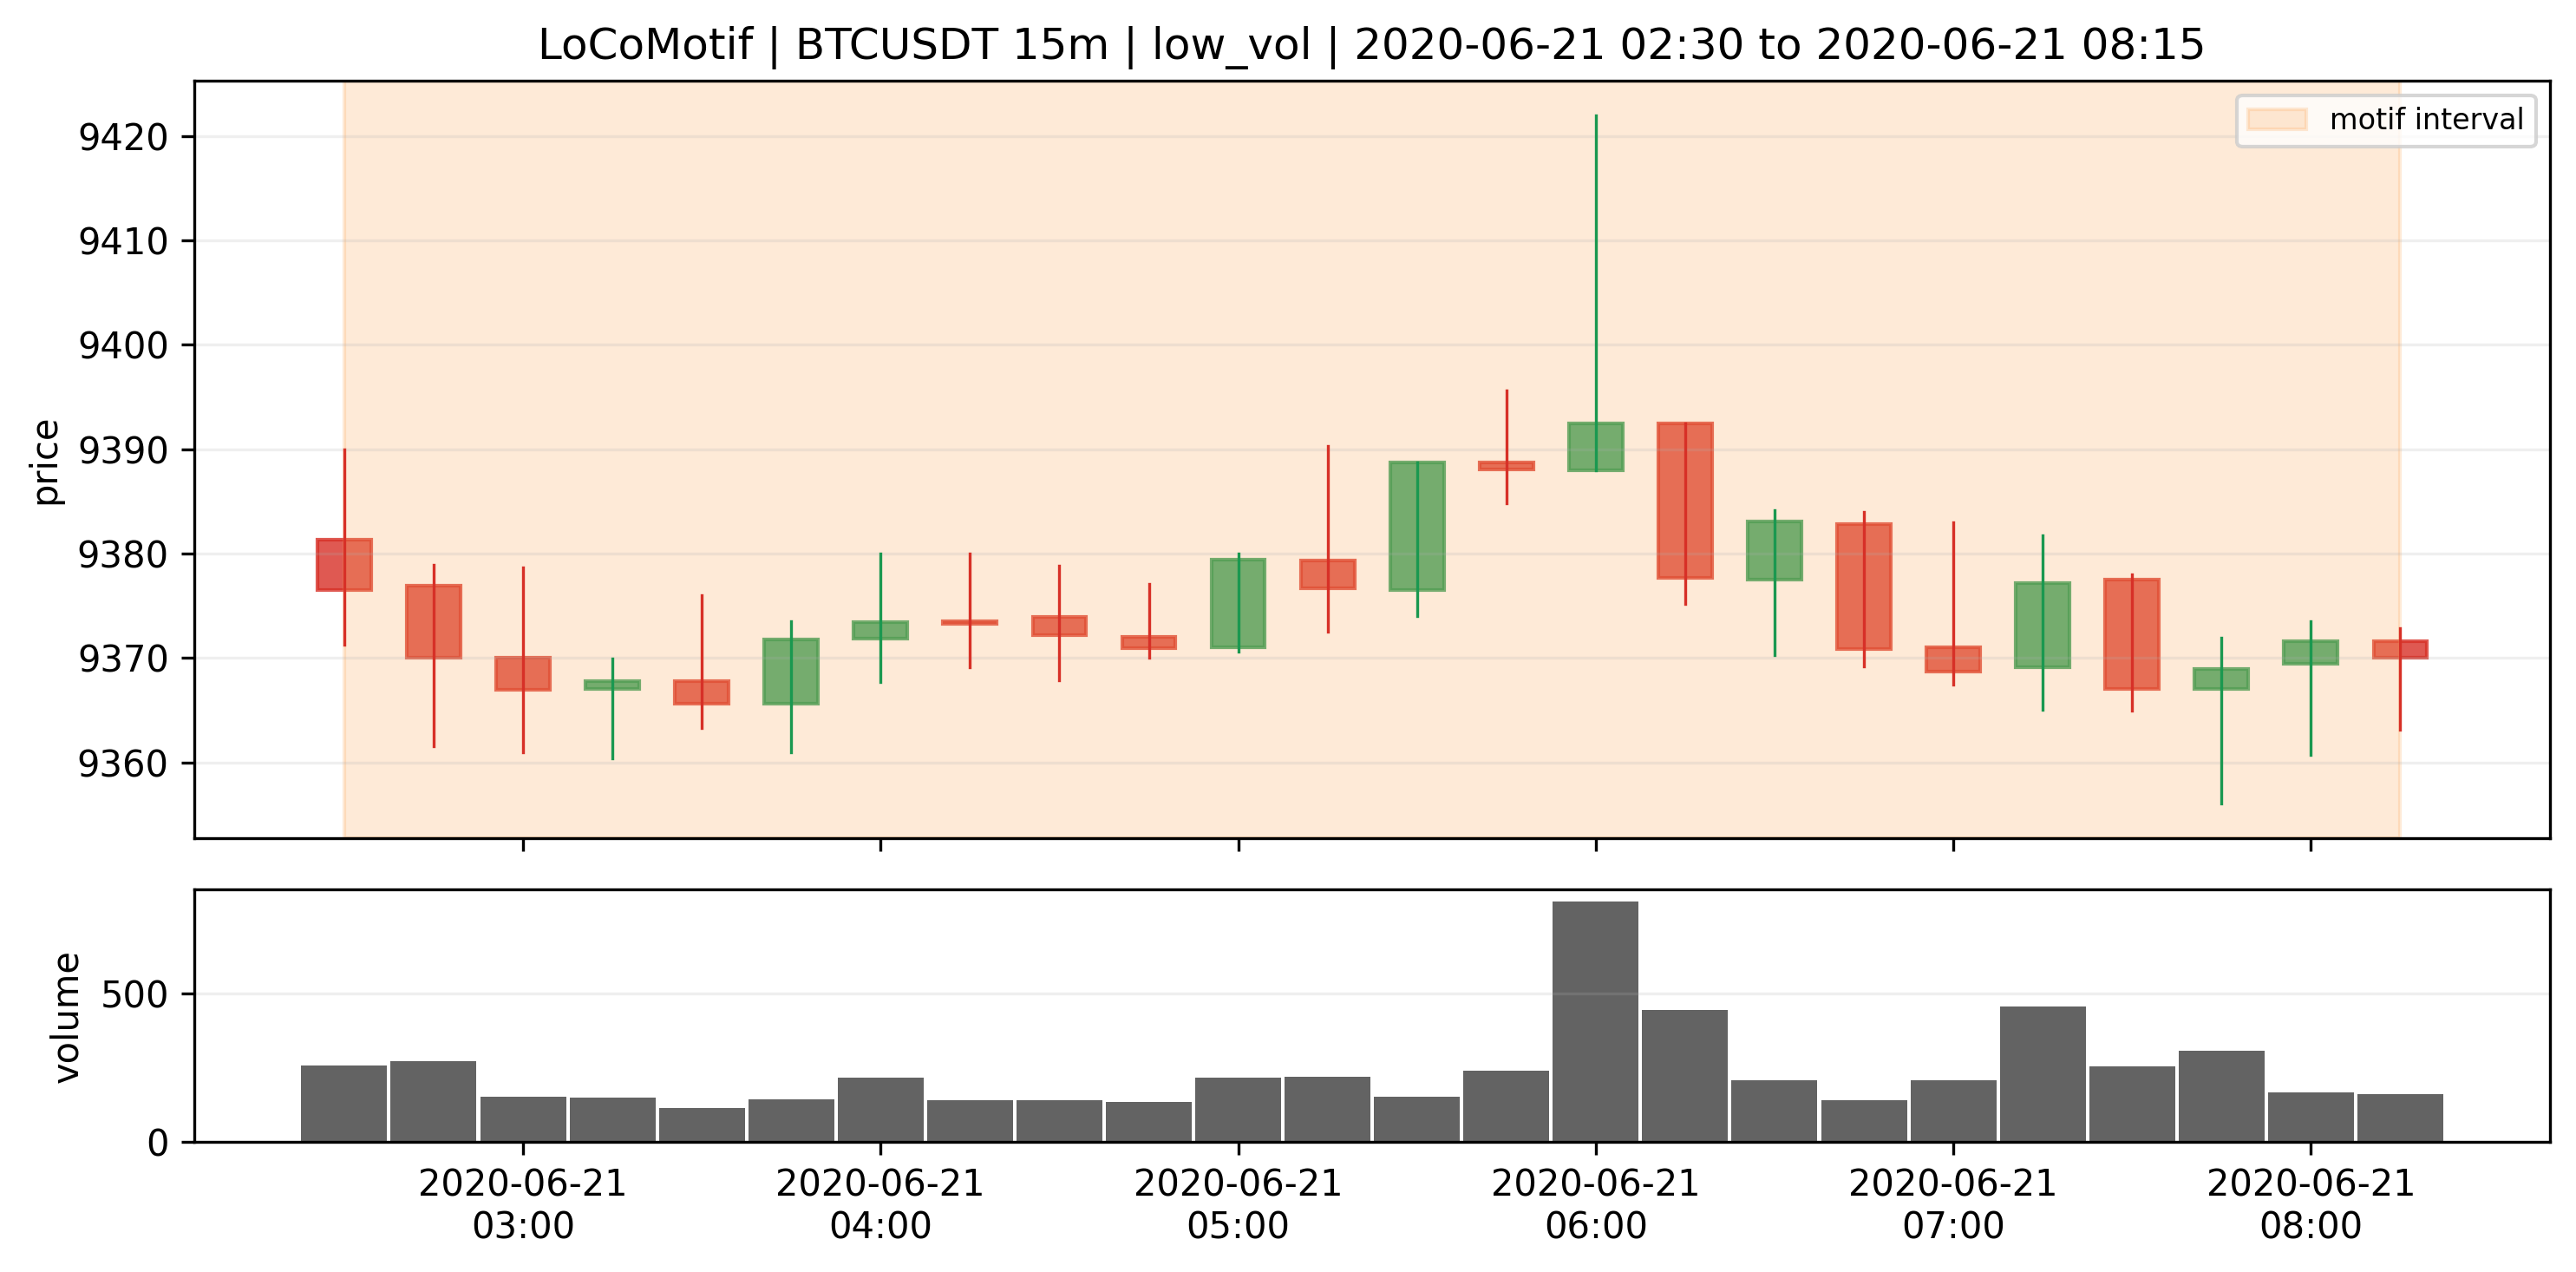
\includegraphics[width=0.9\linewidth]{reports/final_visual_evidence/figures/motif_05_locomotif_btcusdt_15m_low_vol_1_0_1_0_zoom.png}
\caption{motif 05 locomotif btcusdt 15m low vol 1 0 1 0 zoom. The figure compares real available Matrix Profile and LoCoMotif outputs while preserving object-type differences.}
\end{figure}

\begin{figure}[ht]
\centering
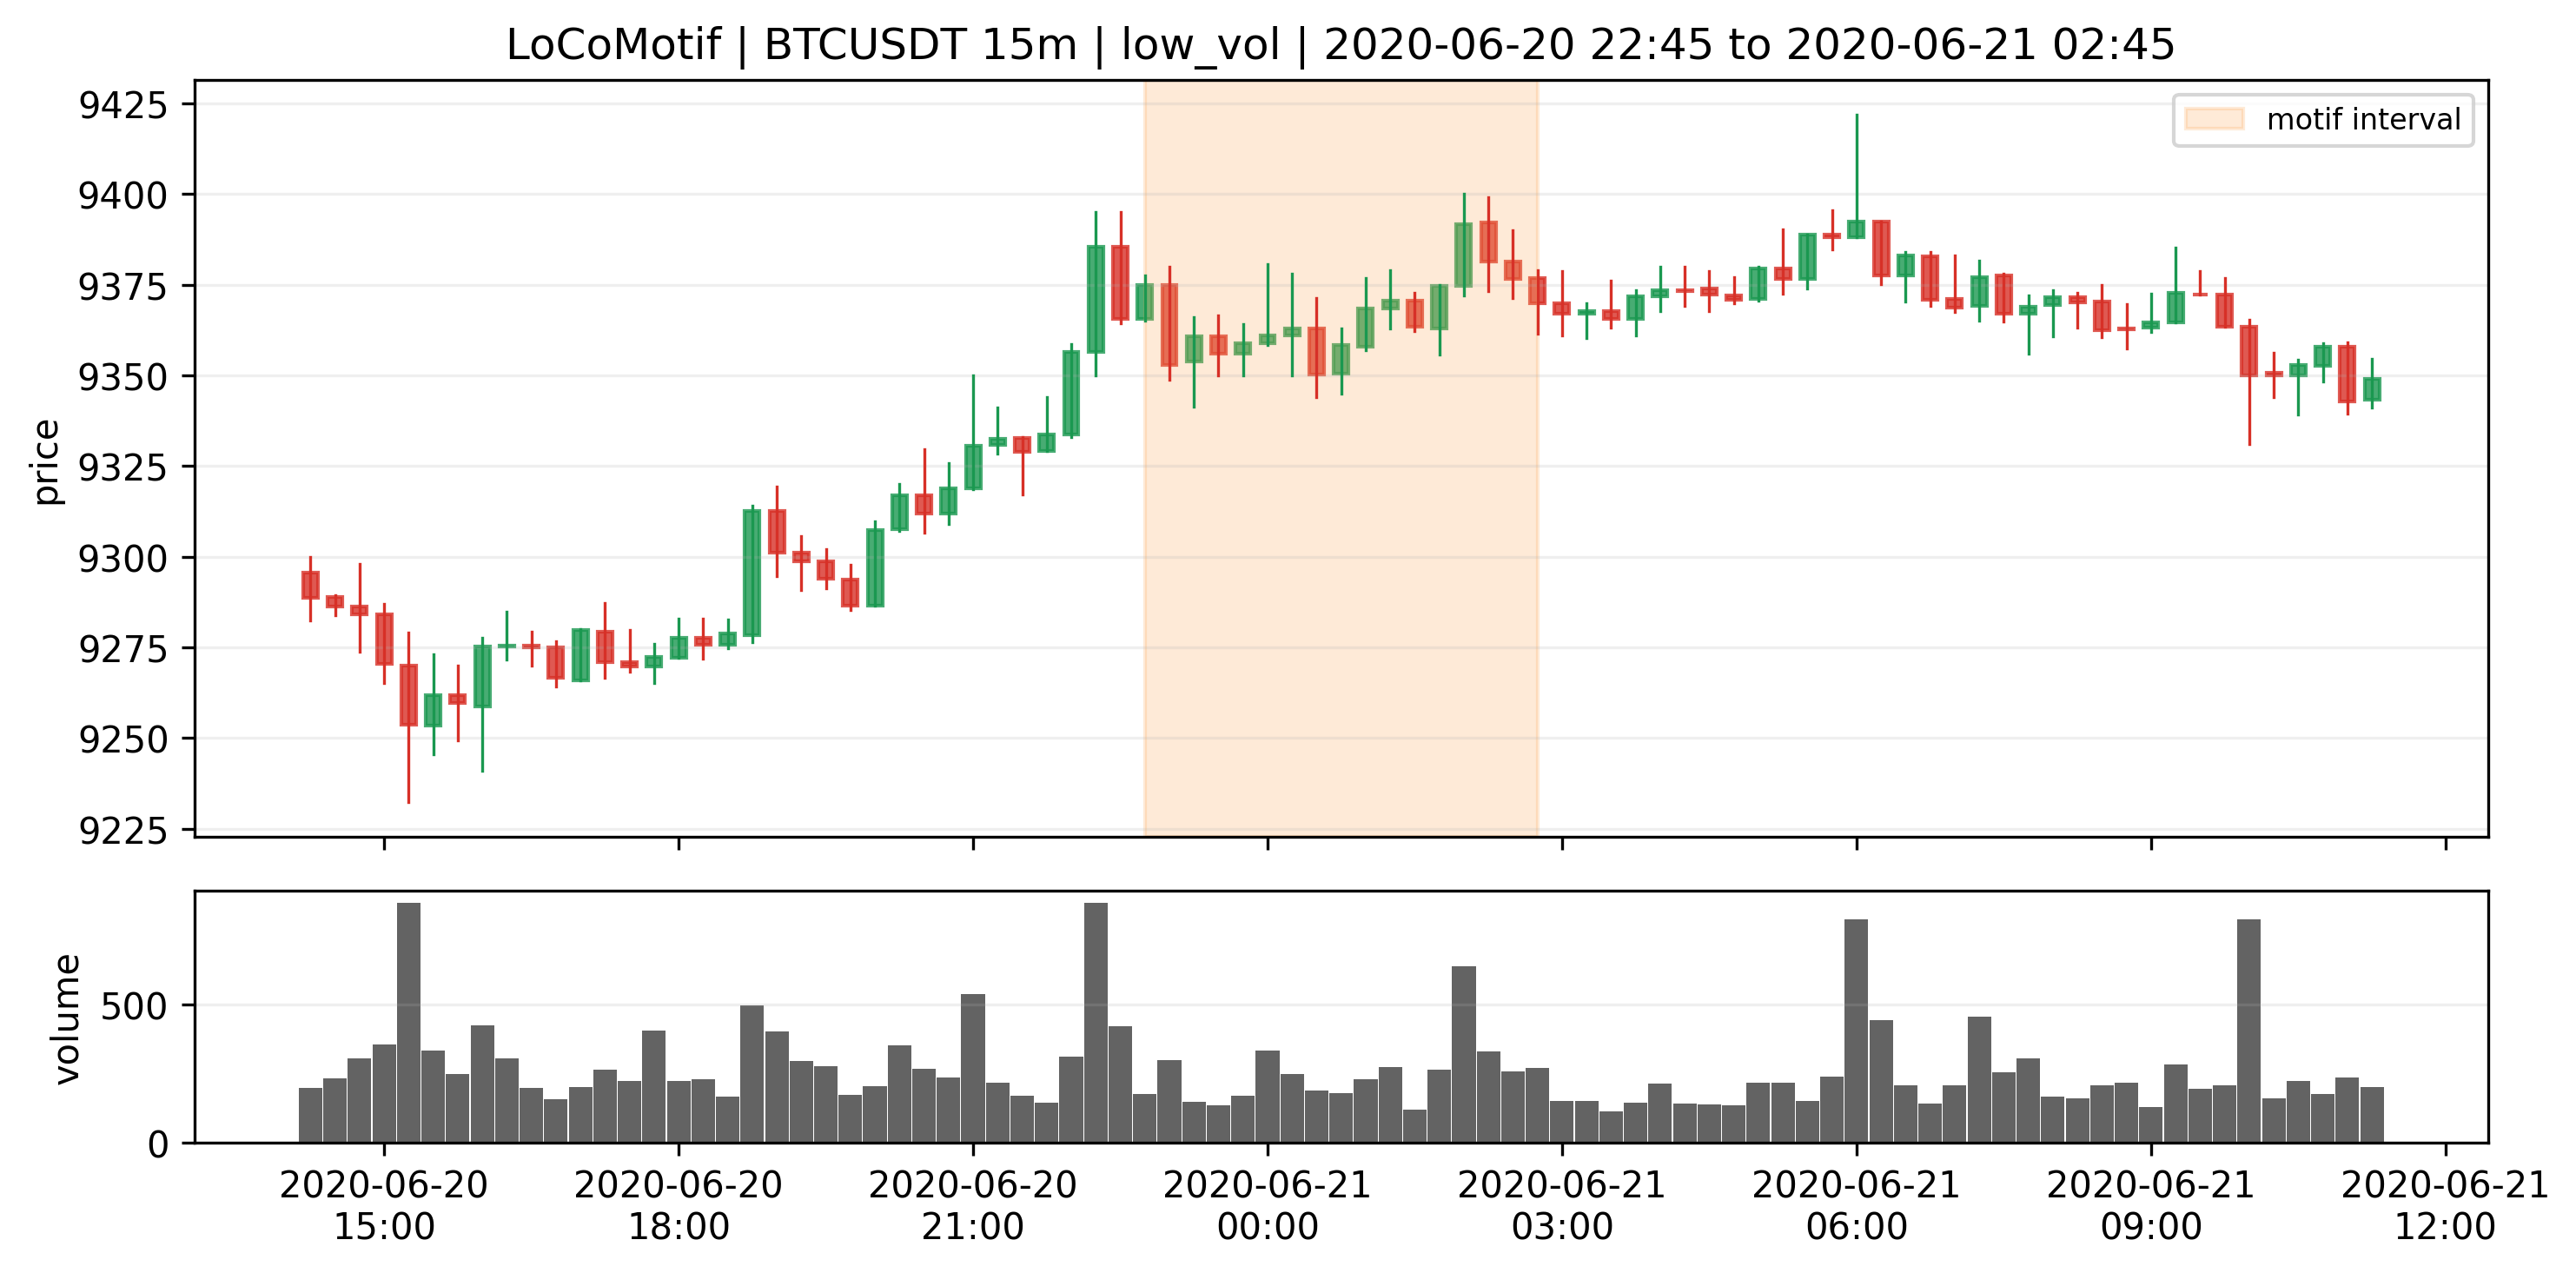
\includegraphics[width=0.9\linewidth]{reports/final_visual_evidence/figures/motif_06_locomotif_btcusdt_15m_low_vol_1_0_3_0_context.png}
\caption{motif 06 locomotif btcusdt 15m low vol 1 0 3 0 context. The figure compares real available Matrix Profile and LoCoMotif outputs while preserving object-type differences.}
\end{figure}

\begin{figure}[ht]
\centering
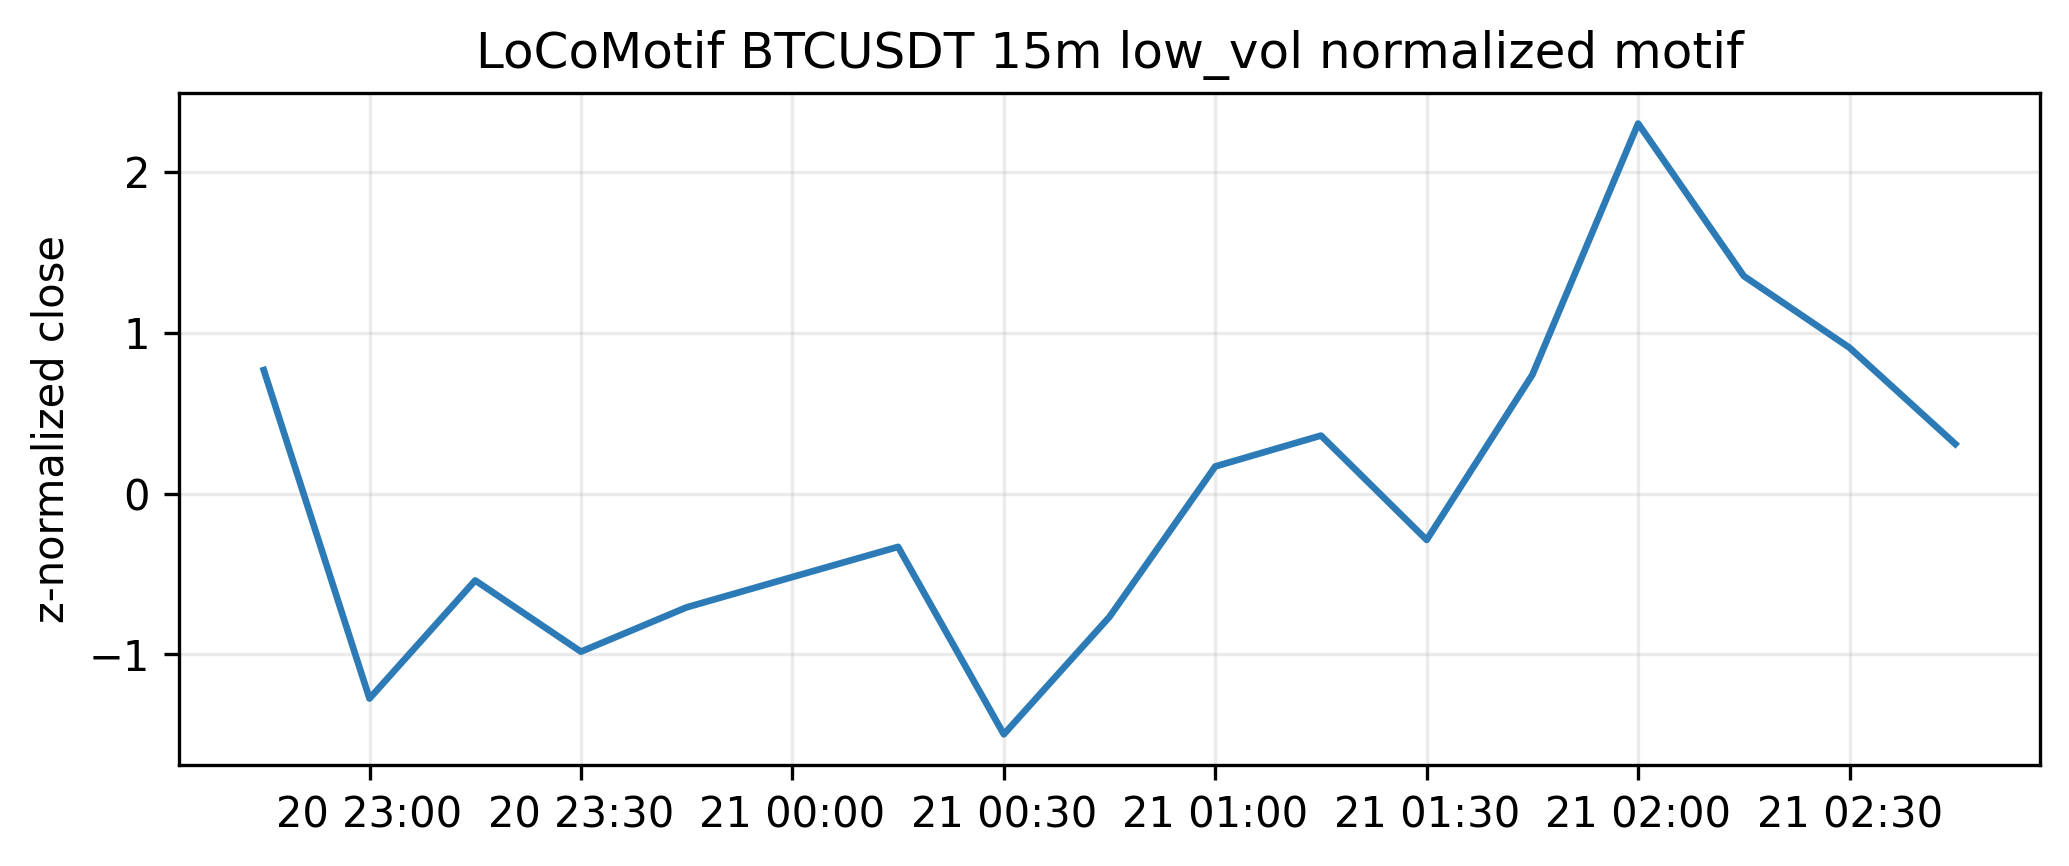
\includegraphics[width=0.9\linewidth]{reports/final_visual_evidence/figures/motif_06_locomotif_btcusdt_15m_low_vol_1_0_3_0_normal_pattern.png}
\caption{motif 06 locomotif btcusdt 15m low vol 1 0 3 0 normal pattern. The figure compares real available Matrix Profile and LoCoMotif outputs while preserving object-type differences.}
\end{figure}

\begin{figure}[ht]
\centering
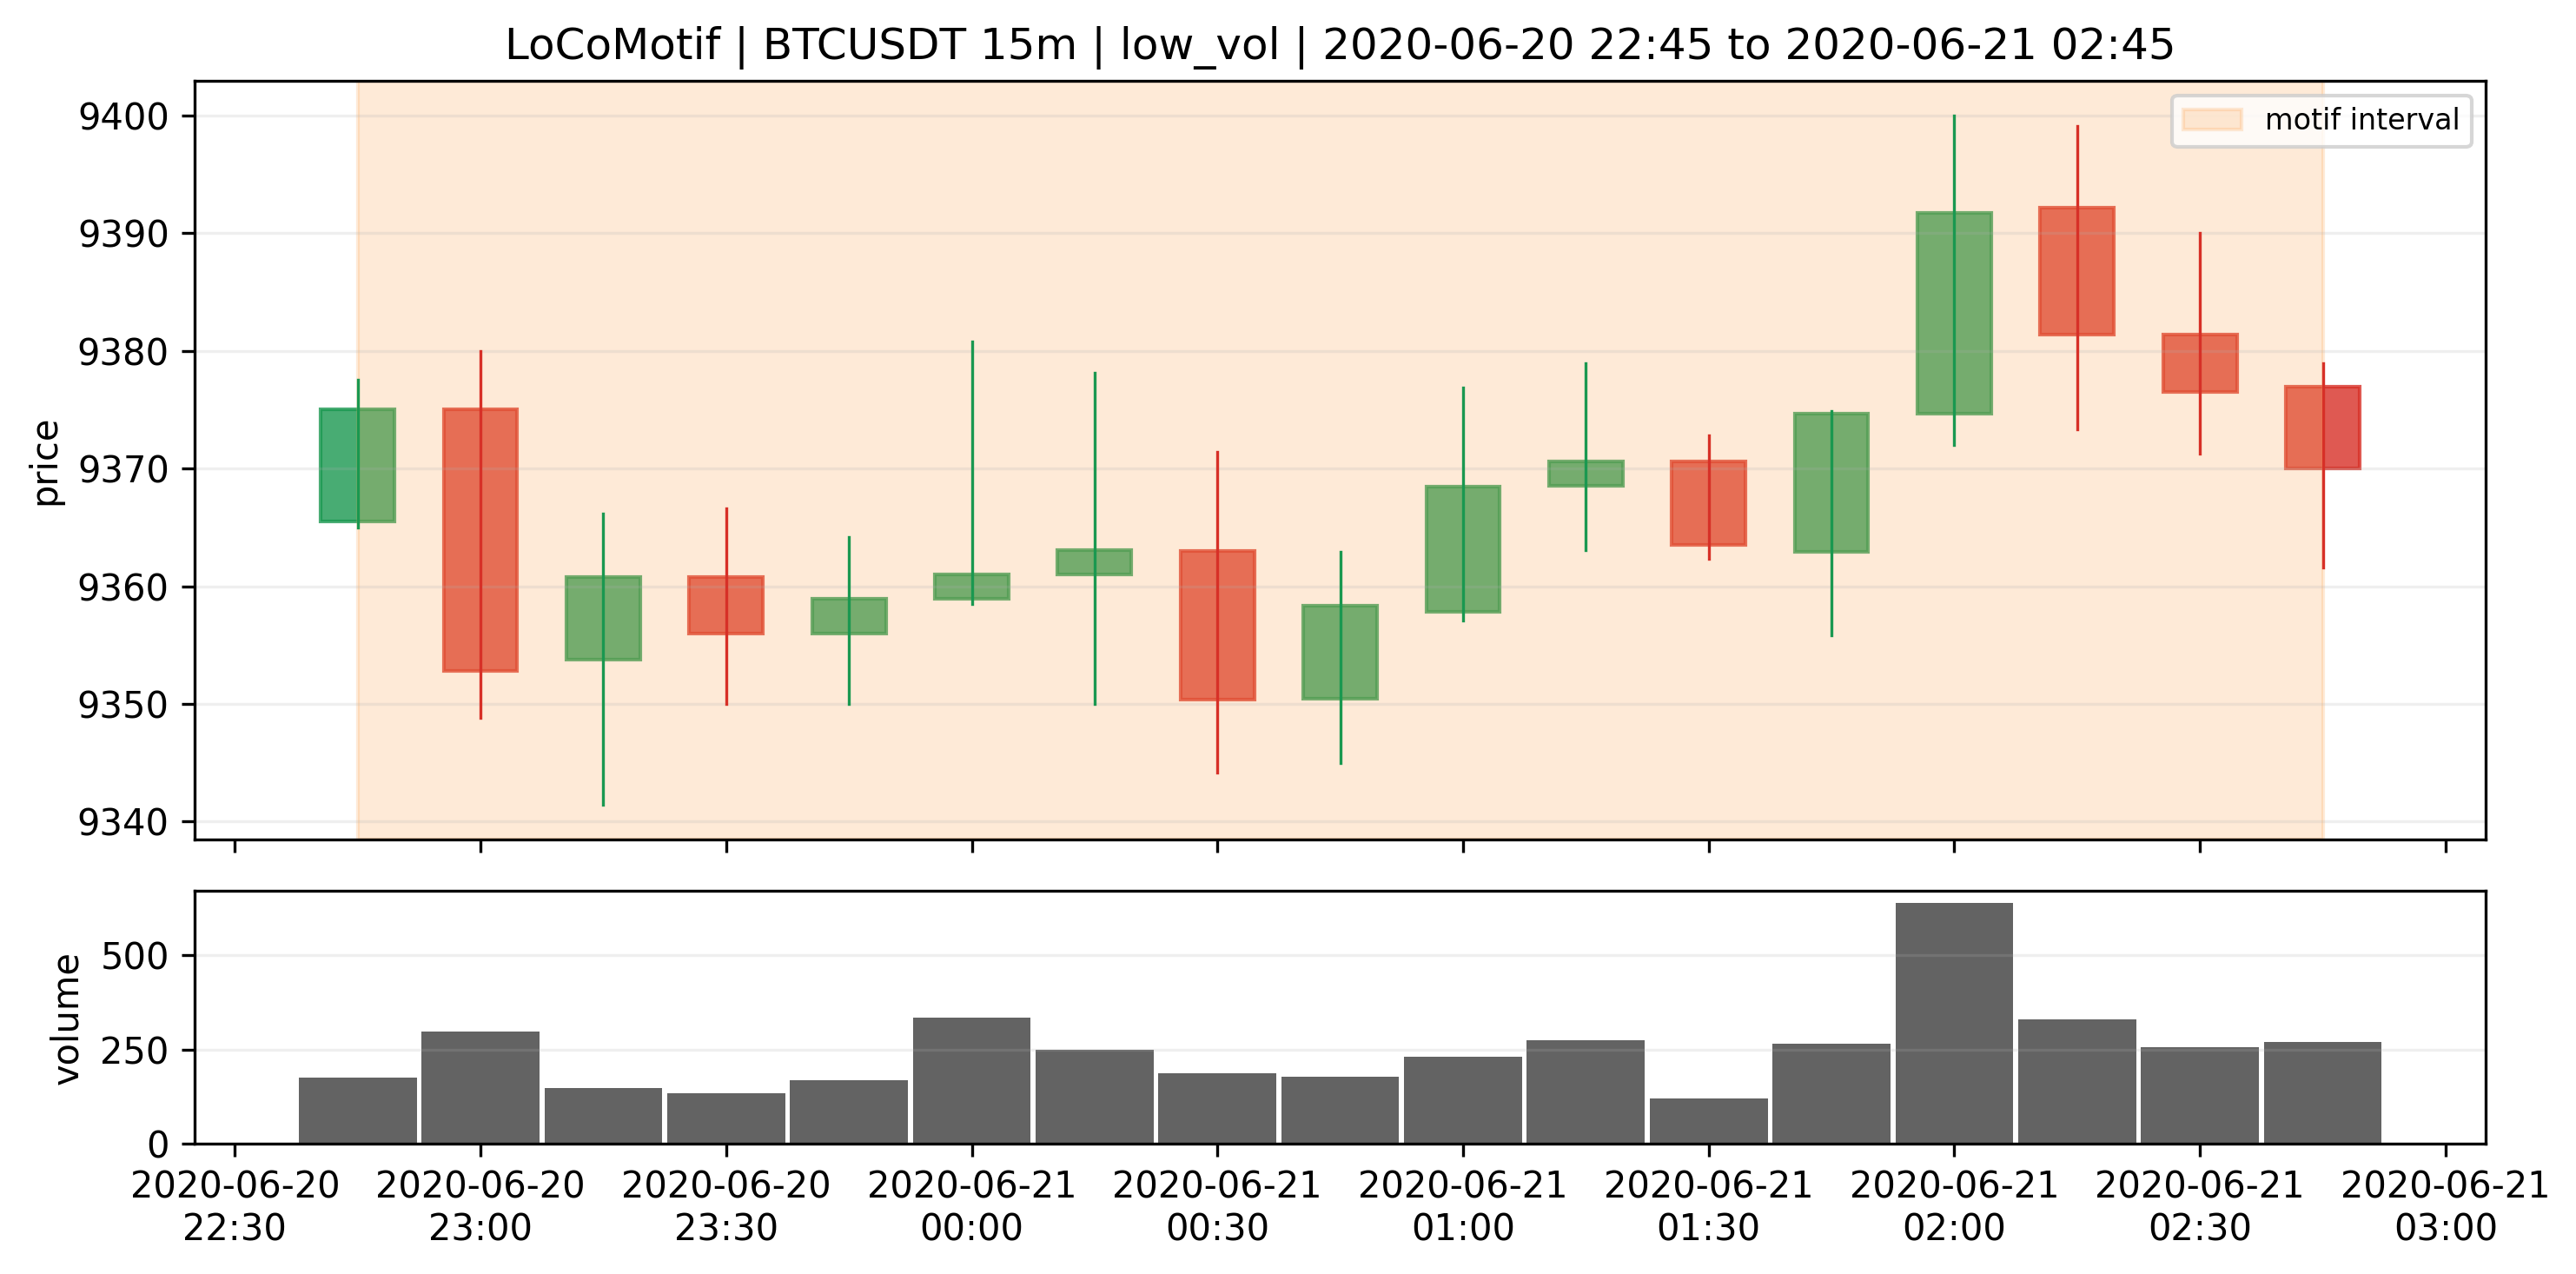
\includegraphics[width=0.9\linewidth]{reports/final_visual_evidence/figures/motif_06_locomotif_btcusdt_15m_low_vol_1_0_3_0_zoom.png}
\caption{motif 06 locomotif btcusdt 15m low vol 1 0 3 0 zoom. The figure compares real available Matrix Profile and LoCoMotif outputs while preserving object-type differences.}
\end{figure}

\begin{figure}[ht]
\centering
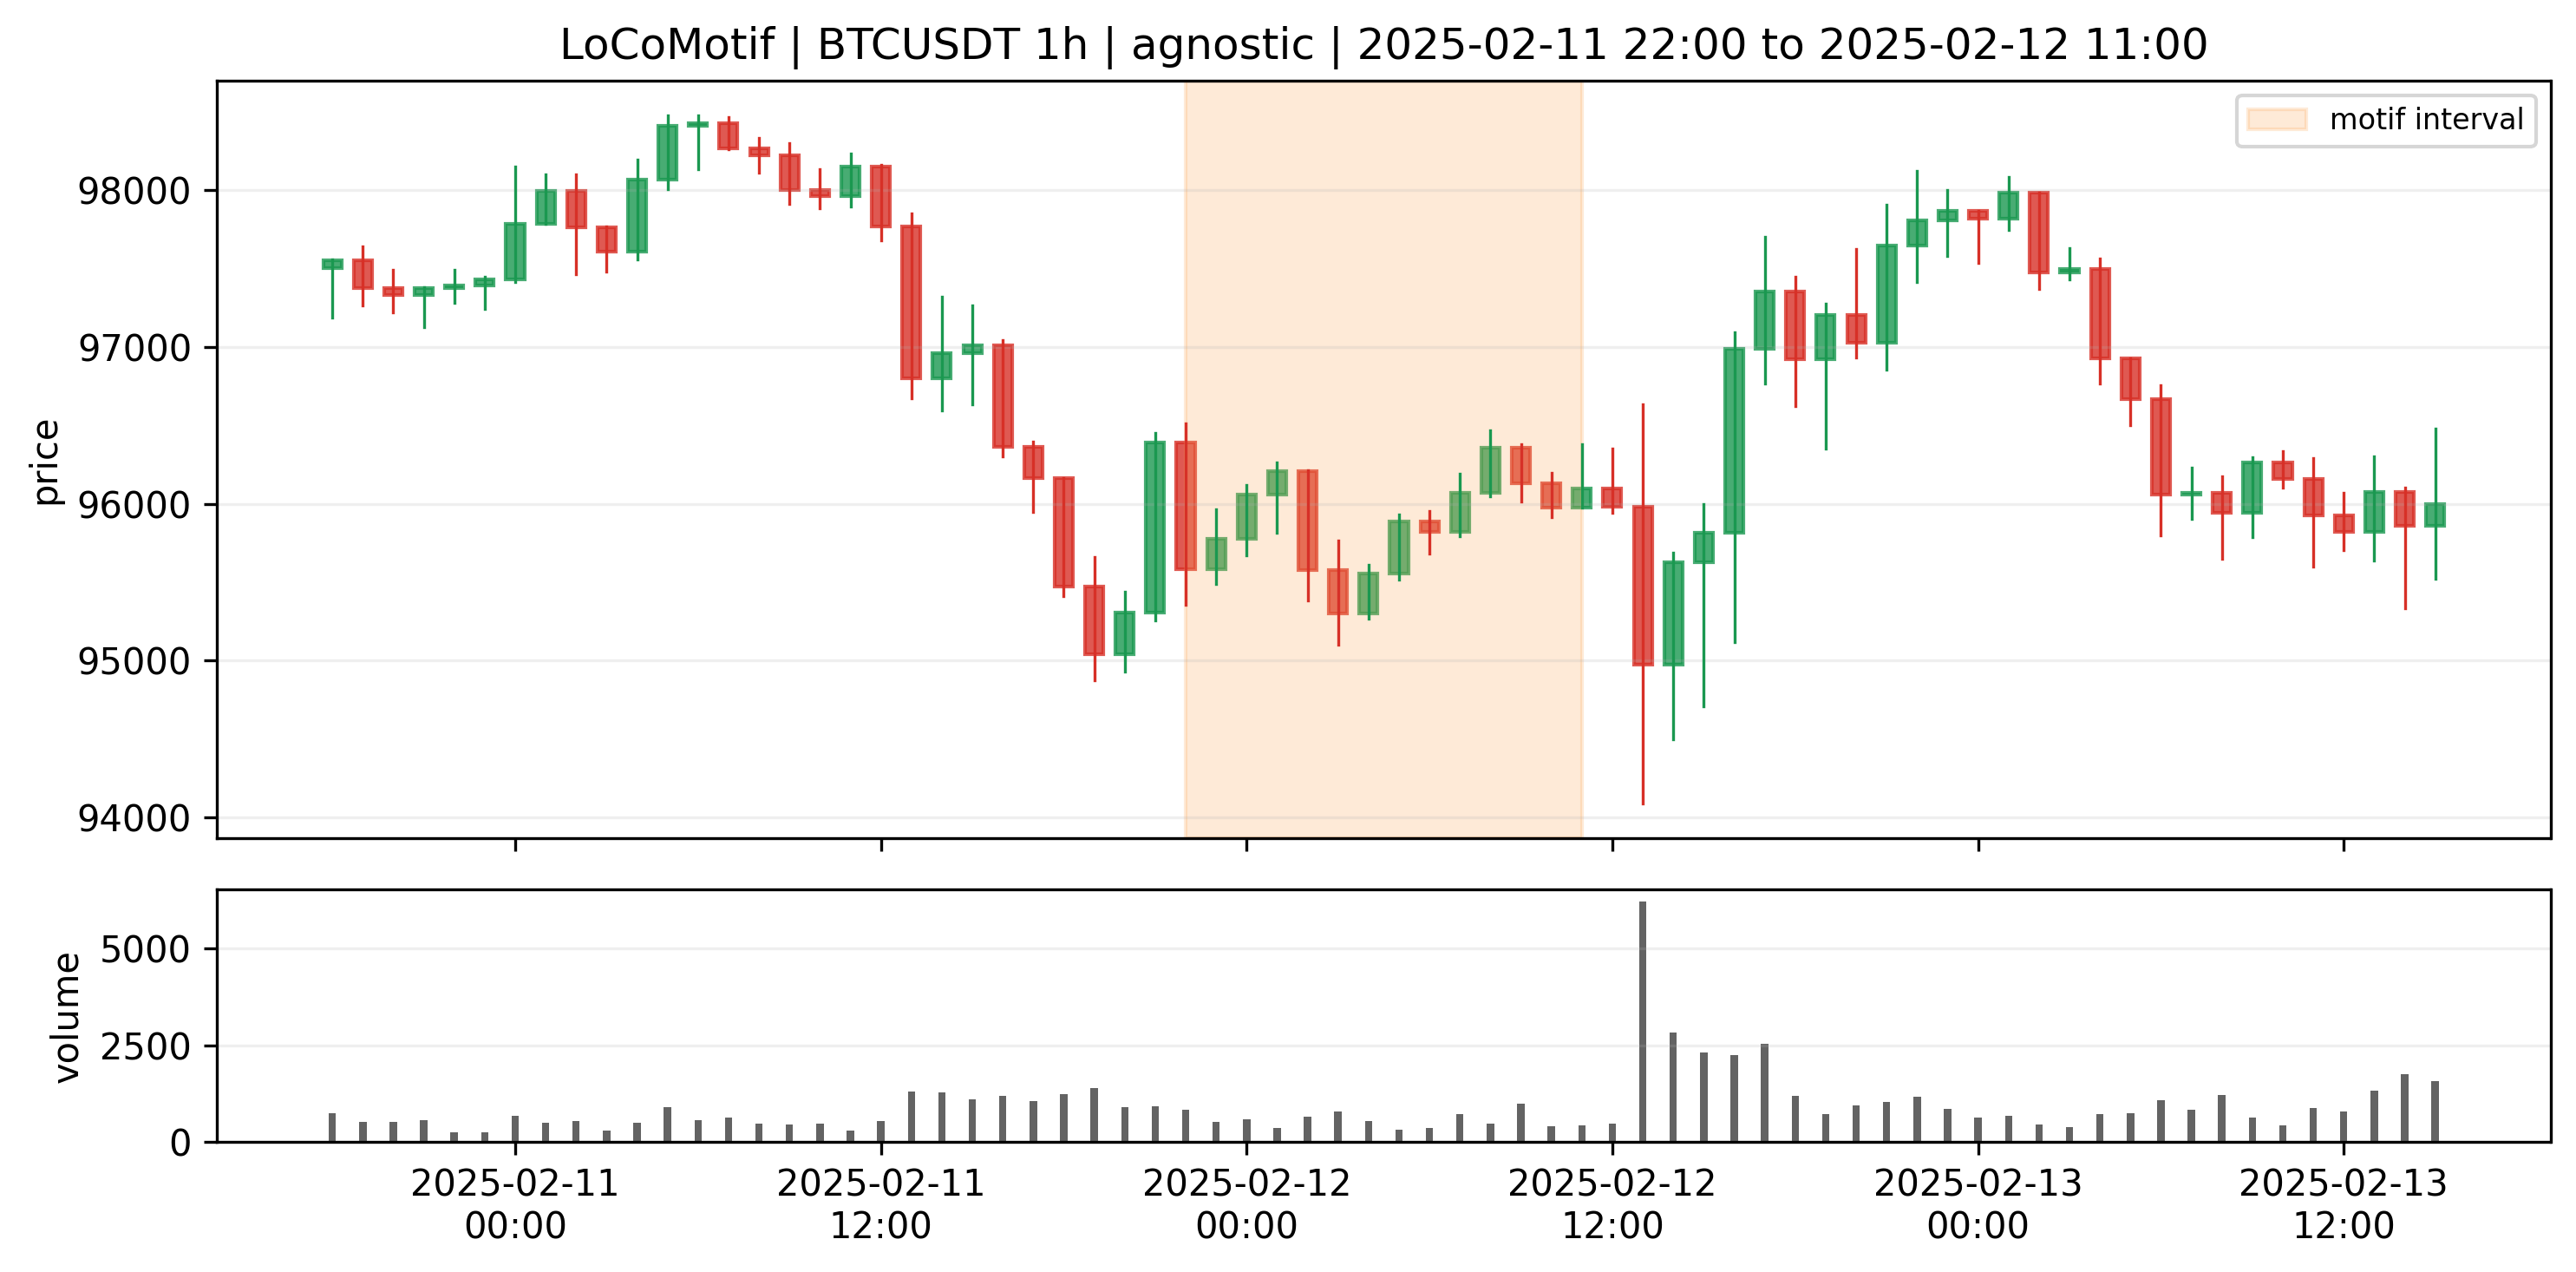
\includegraphics[width=0.9\linewidth]{reports/final_visual_evidence/figures/motif_07_locomotif_btcusdt_1h_agnostic_nan_nan_context.png}
\caption{motif 07 locomotif btcusdt 1h agnostic nan nan context. The figure compares real available Matrix Profile and LoCoMotif outputs while preserving object-type differences.}
\end{figure}

\begin{figure}[ht]
\centering
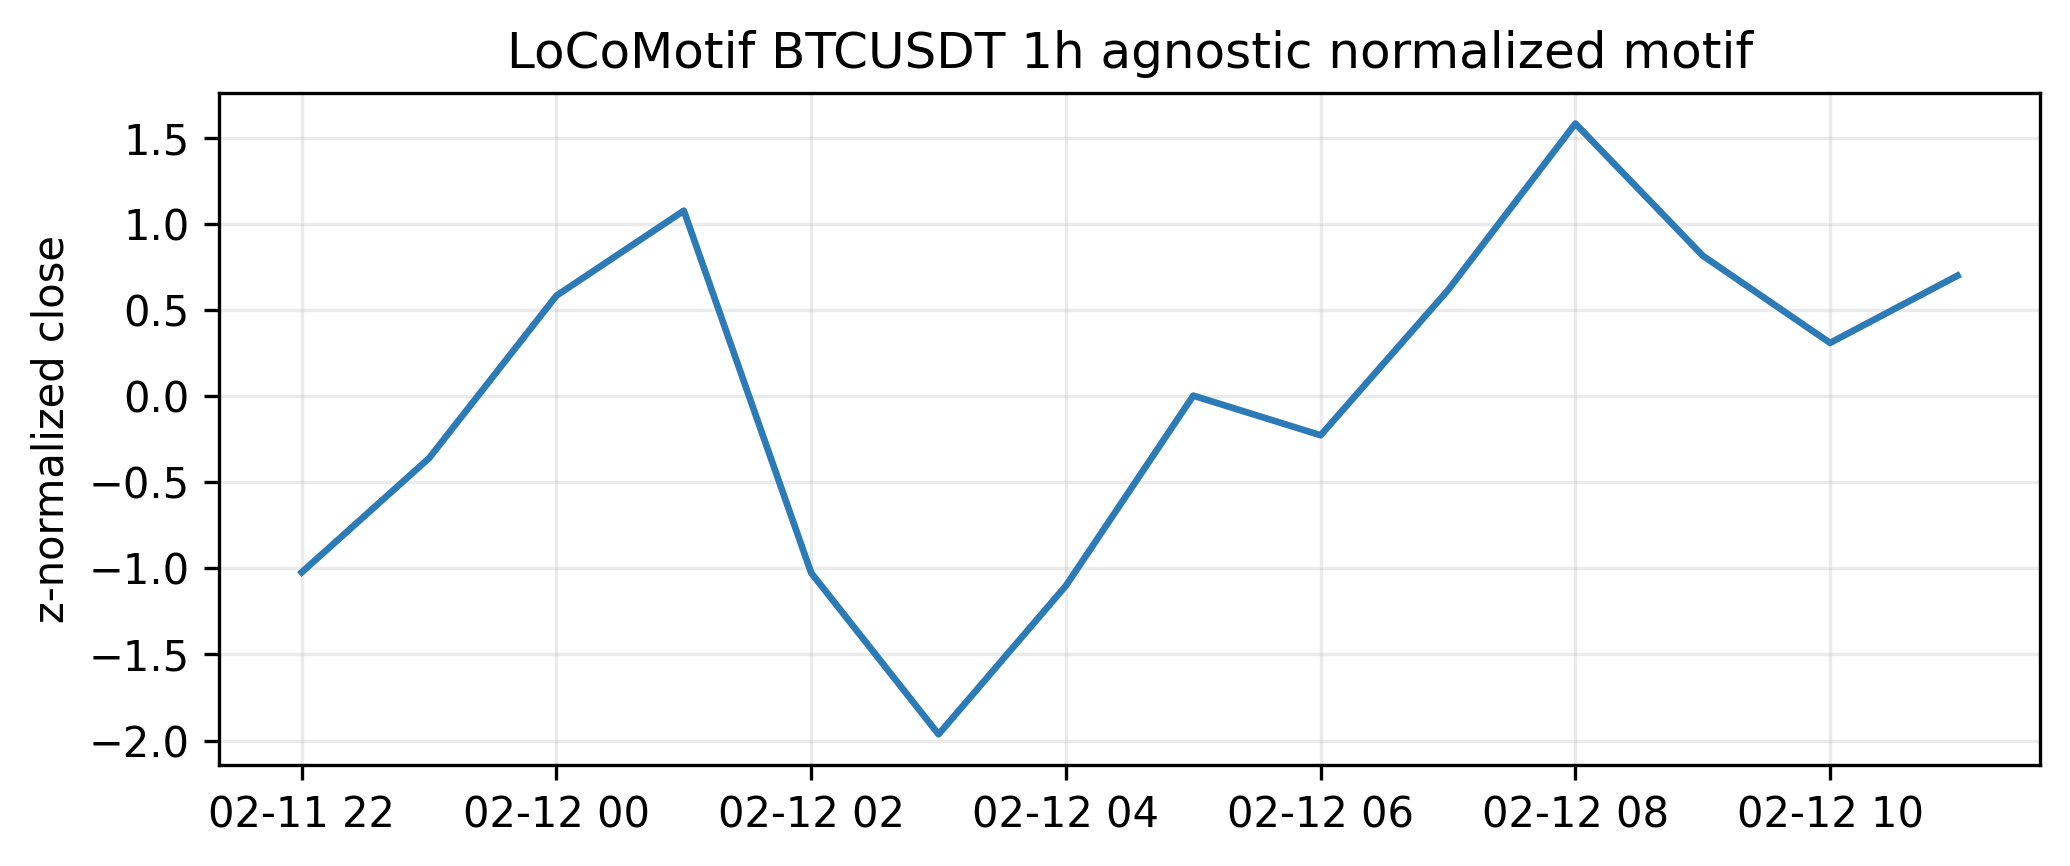
\includegraphics[width=0.9\linewidth]{reports/final_visual_evidence/figures/motif_07_locomotif_btcusdt_1h_agnostic_nan_nan_normal_pattern.png}
\caption{motif 07 locomotif btcusdt 1h agnostic nan nan normal pattern. The figure compares real available Matrix Profile and LoCoMotif outputs while preserving object-type differences.}
\end{figure}

\begin{figure}[ht]
\centering
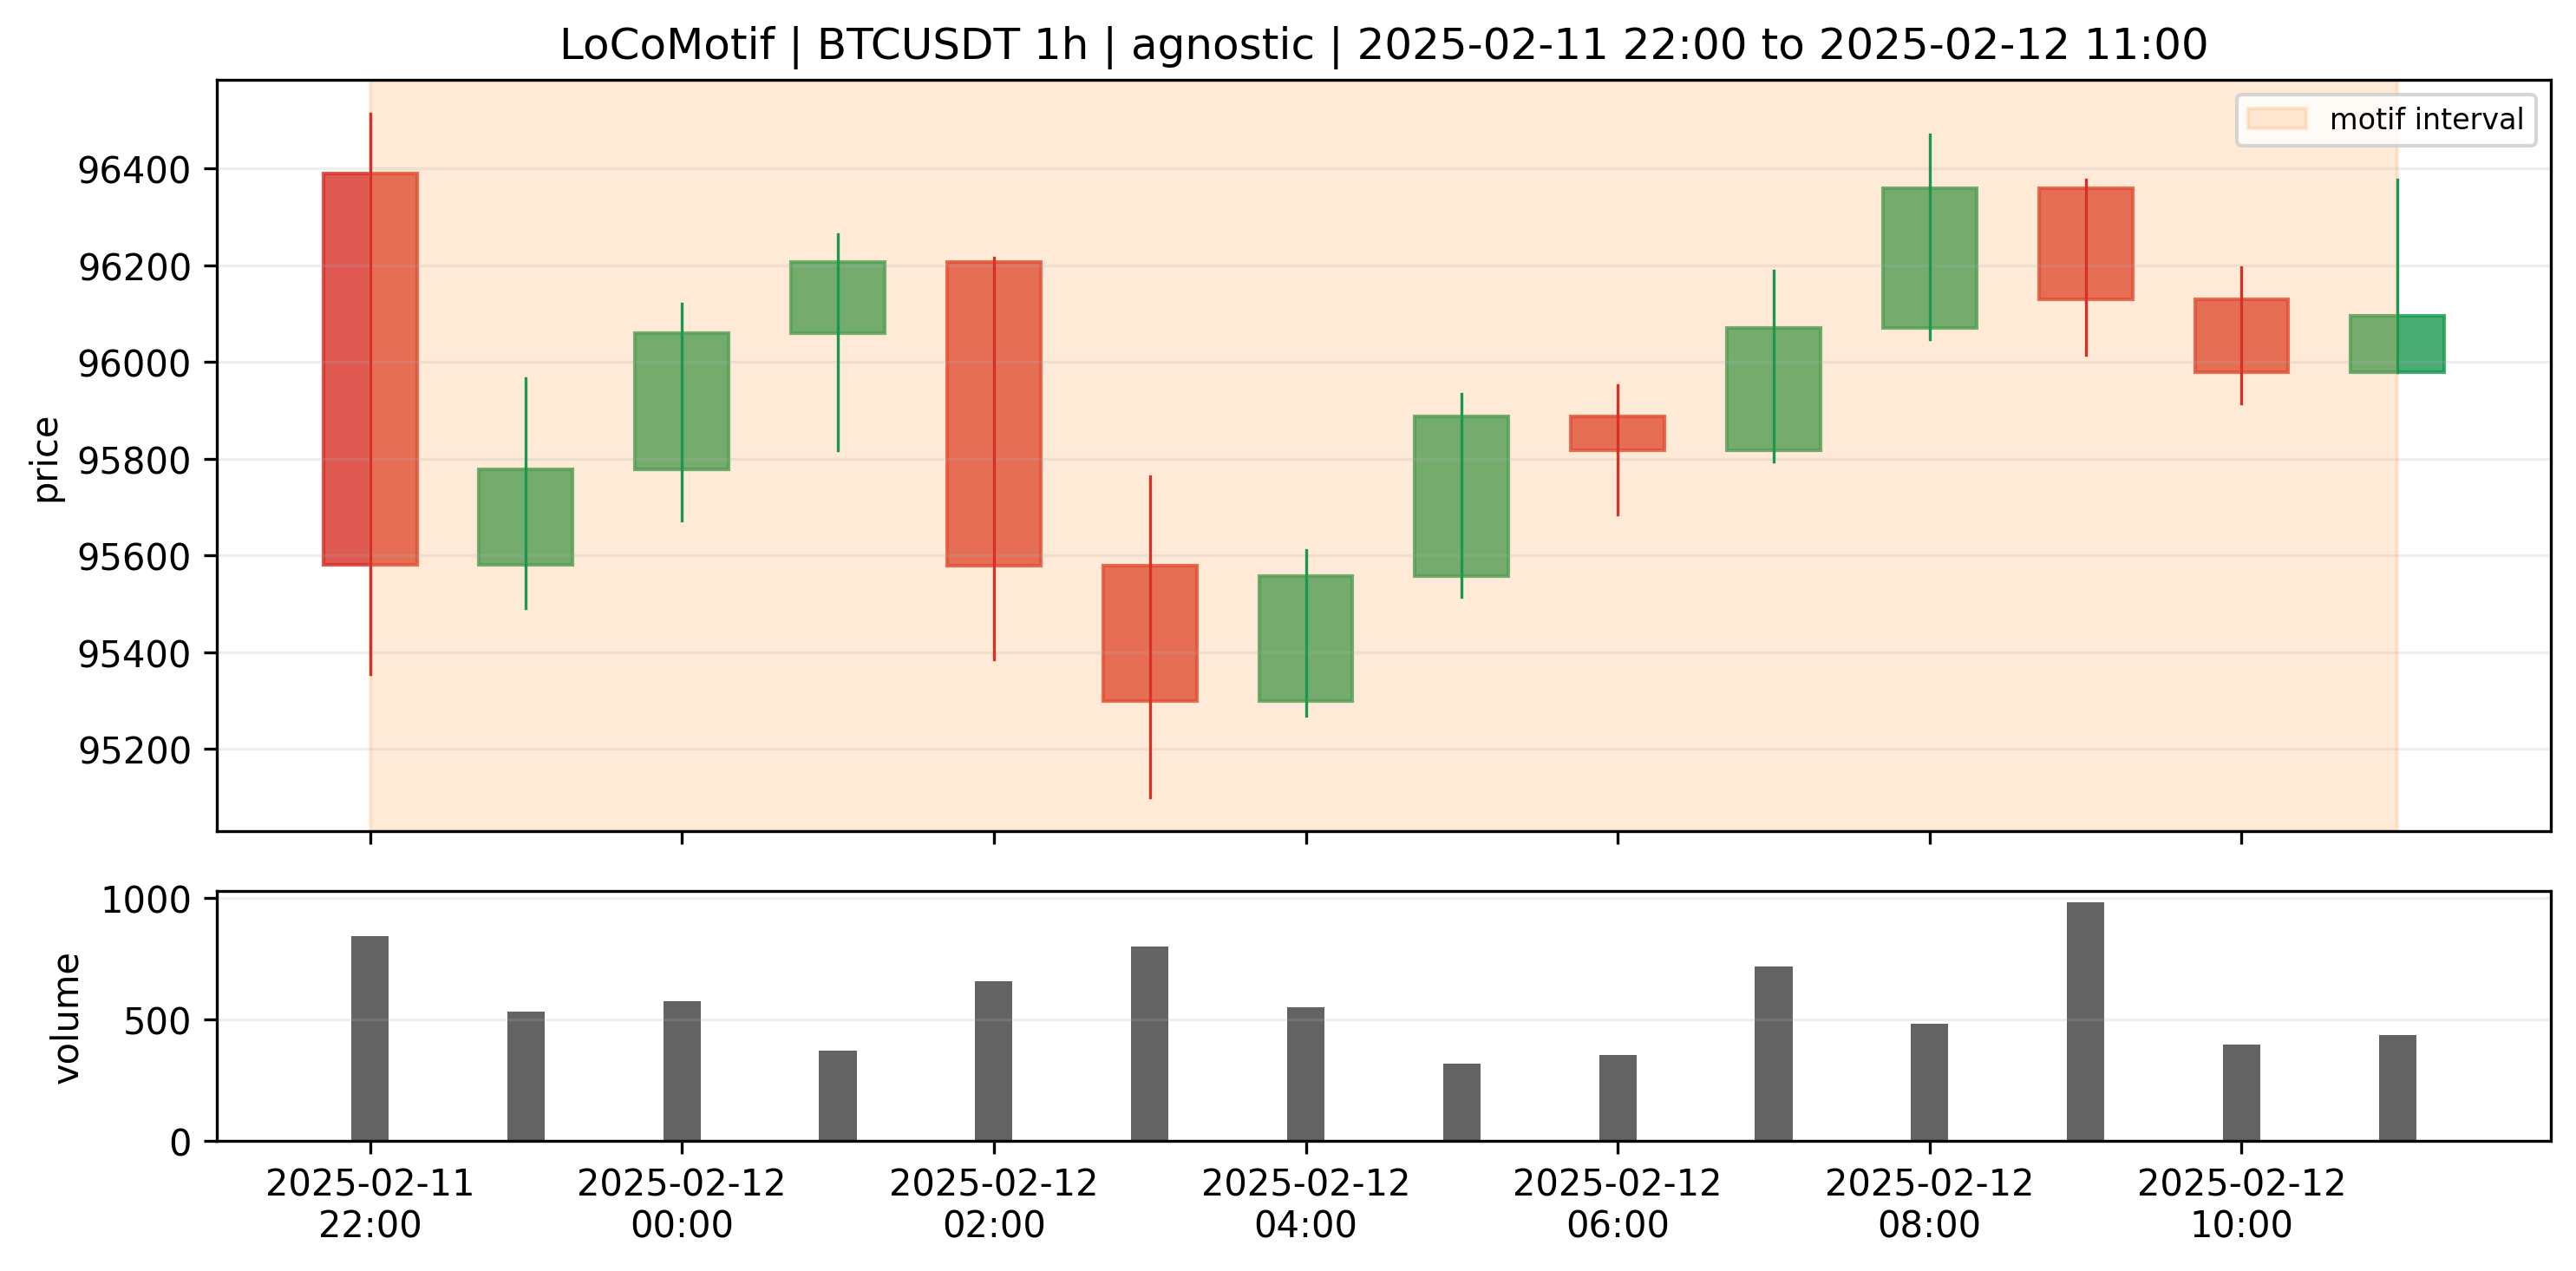
\includegraphics[width=0.9\linewidth]{reports/final_visual_evidence/figures/motif_07_locomotif_btcusdt_1h_agnostic_nan_nan_zoom.png}
\caption{motif 07 locomotif btcusdt 1h agnostic nan nan zoom. The figure compares real available Matrix Profile and LoCoMotif outputs while preserving object-type differences.}
\end{figure}

\begin{figure}[ht]
\centering
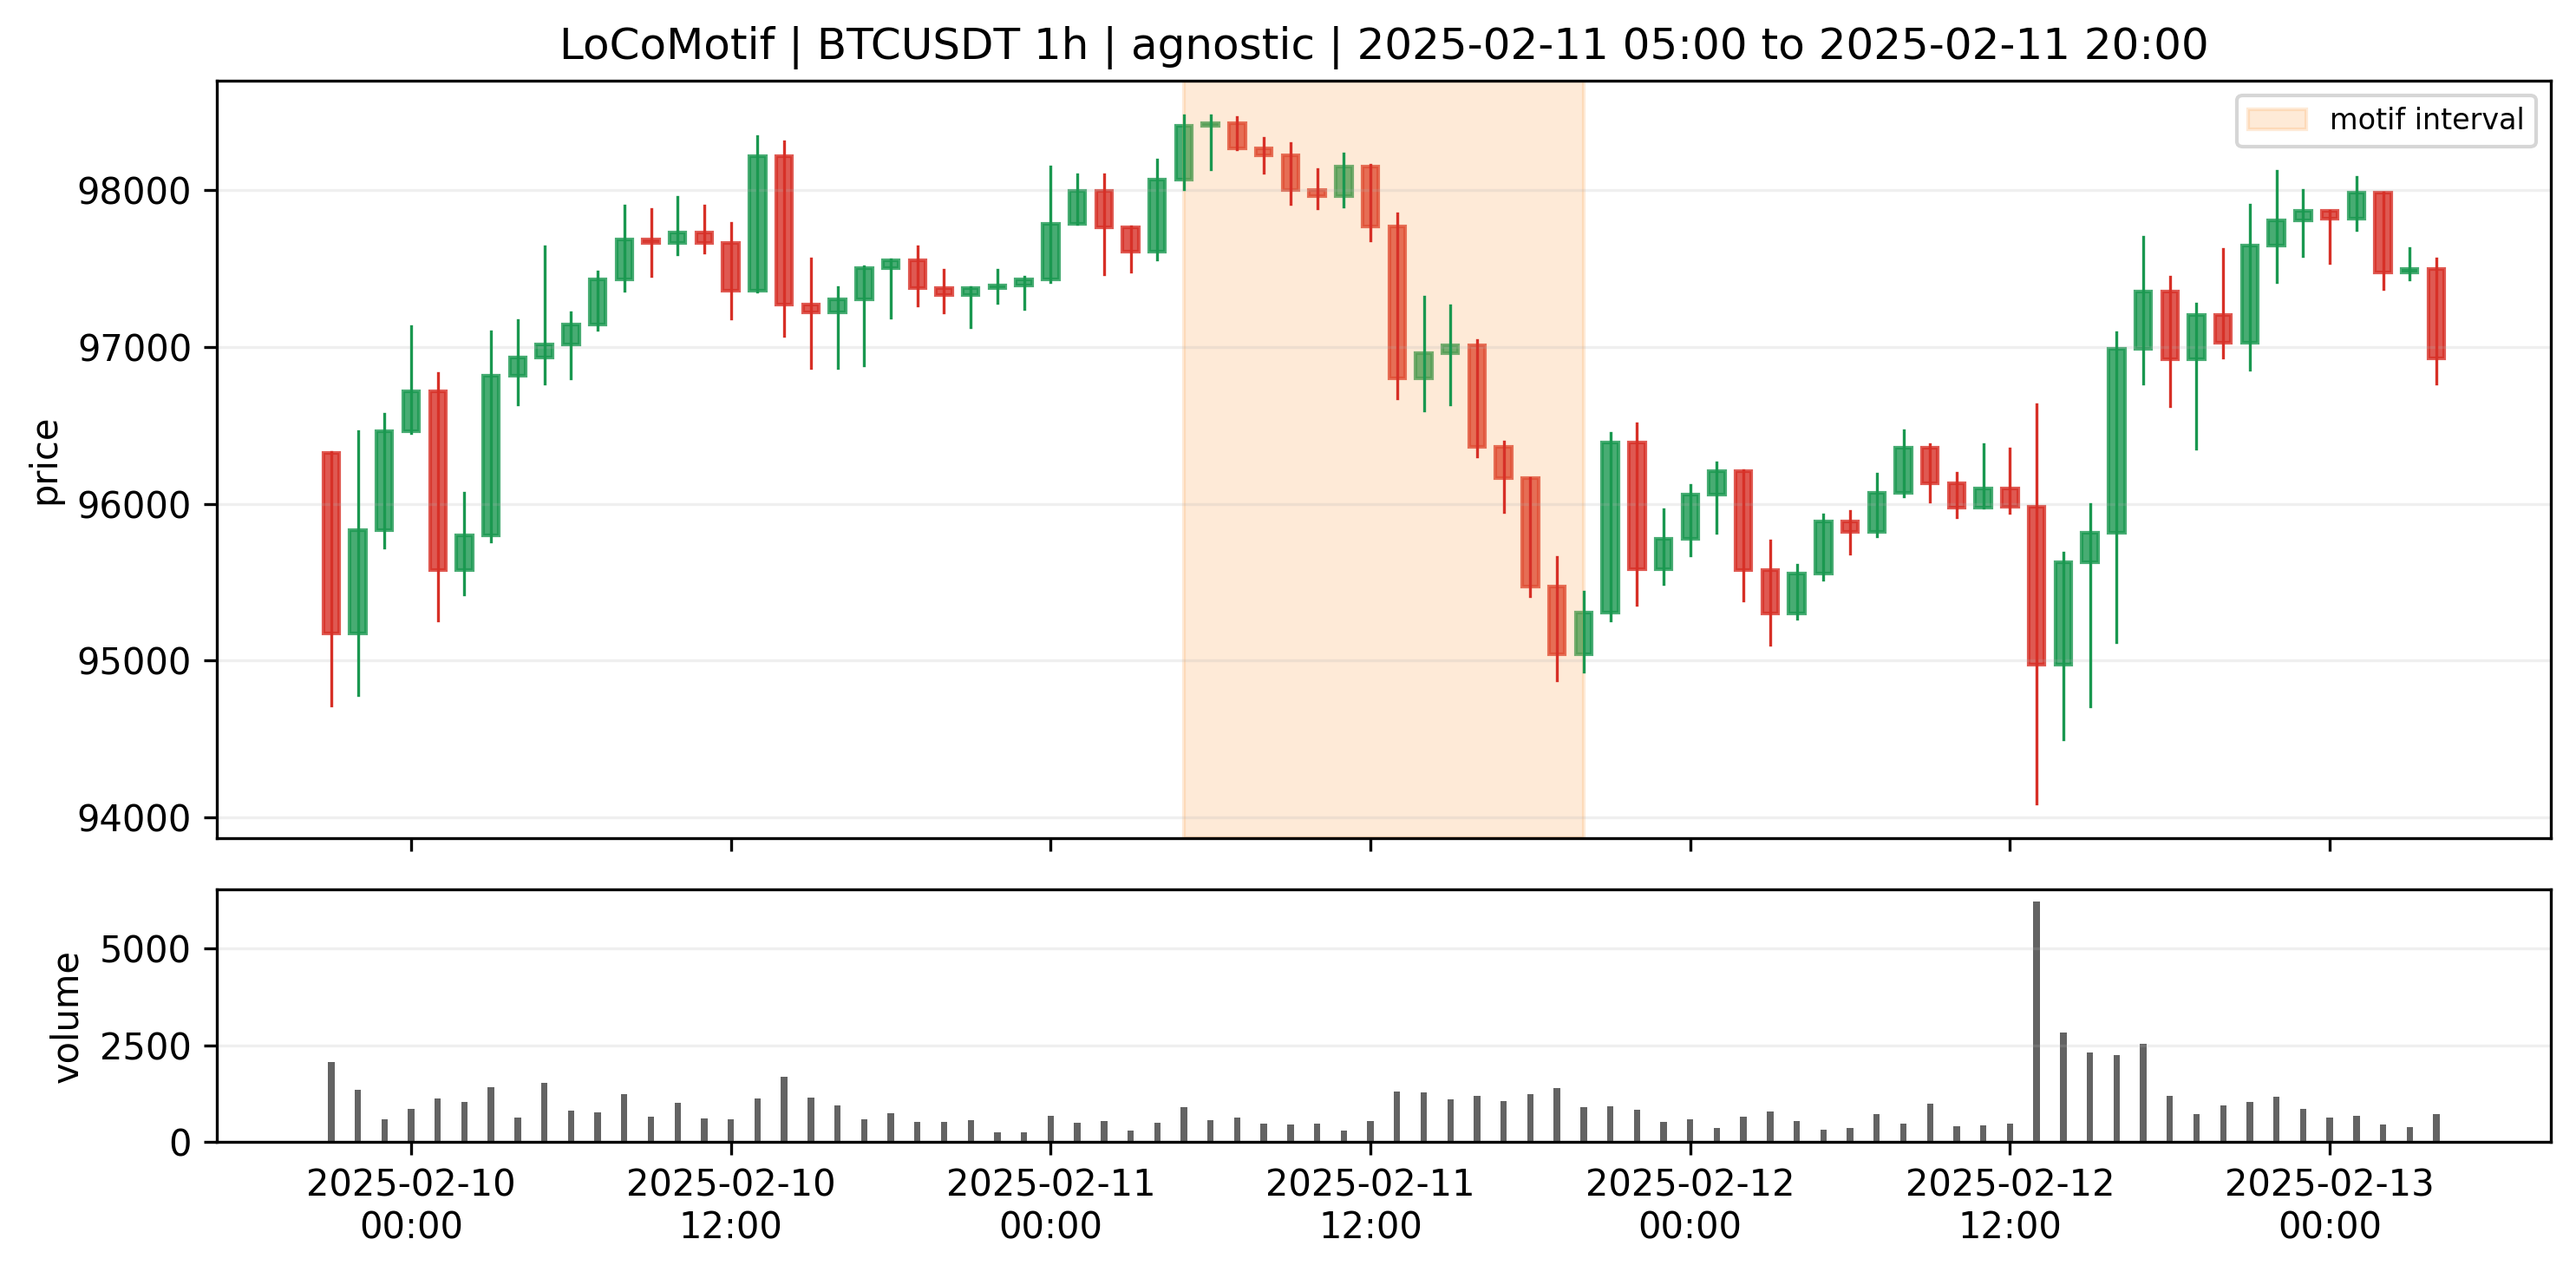
\includegraphics[width=0.9\linewidth]{reports/final_visual_evidence/figures/motif_08_locomotif_btcusdt_1h_agnostic_nan_nan_context.png}
\caption{motif 08 locomotif btcusdt 1h agnostic nan nan context. The figure compares real available Matrix Profile and LoCoMotif outputs while preserving object-type differences.}
\end{figure}

\begin{figure}[ht]
\centering
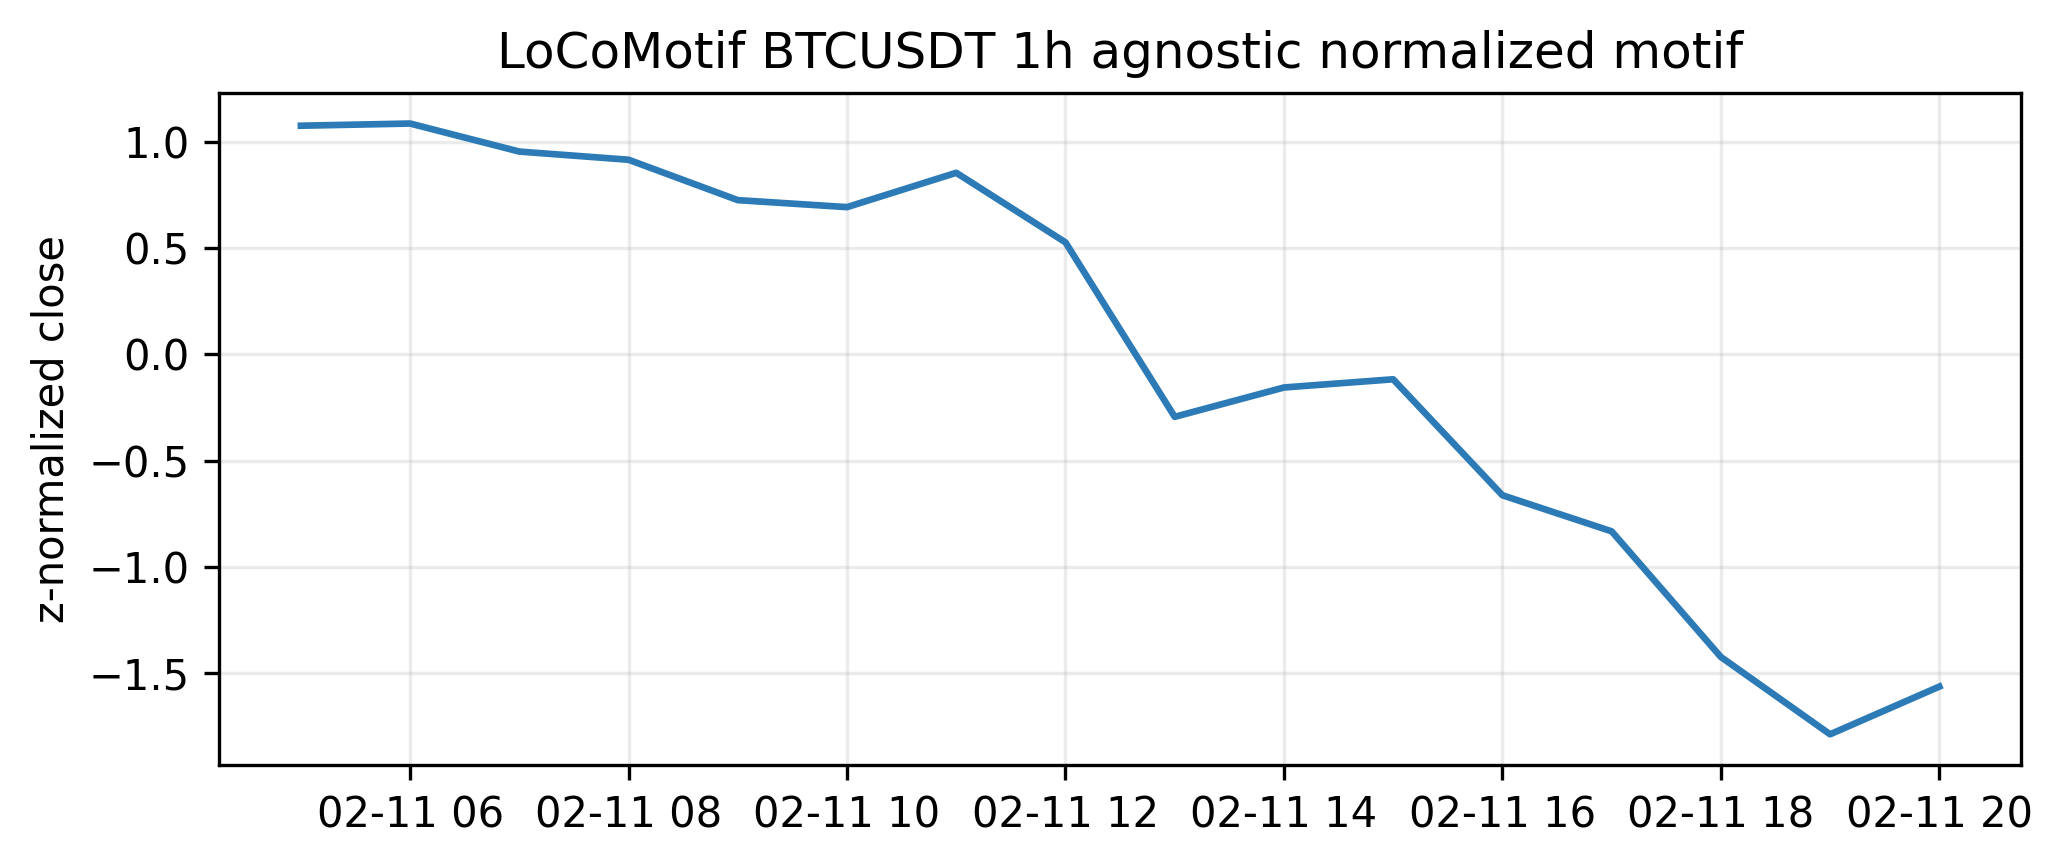
\includegraphics[width=0.9\linewidth]{reports/final_visual_evidence/figures/motif_08_locomotif_btcusdt_1h_agnostic_nan_nan_normal_pattern.png}
\caption{motif 08 locomotif btcusdt 1h agnostic nan nan normal pattern. The figure compares real available Matrix Profile and LoCoMotif outputs while preserving object-type differences.}
\end{figure}

\begin{figure}[ht]
\centering
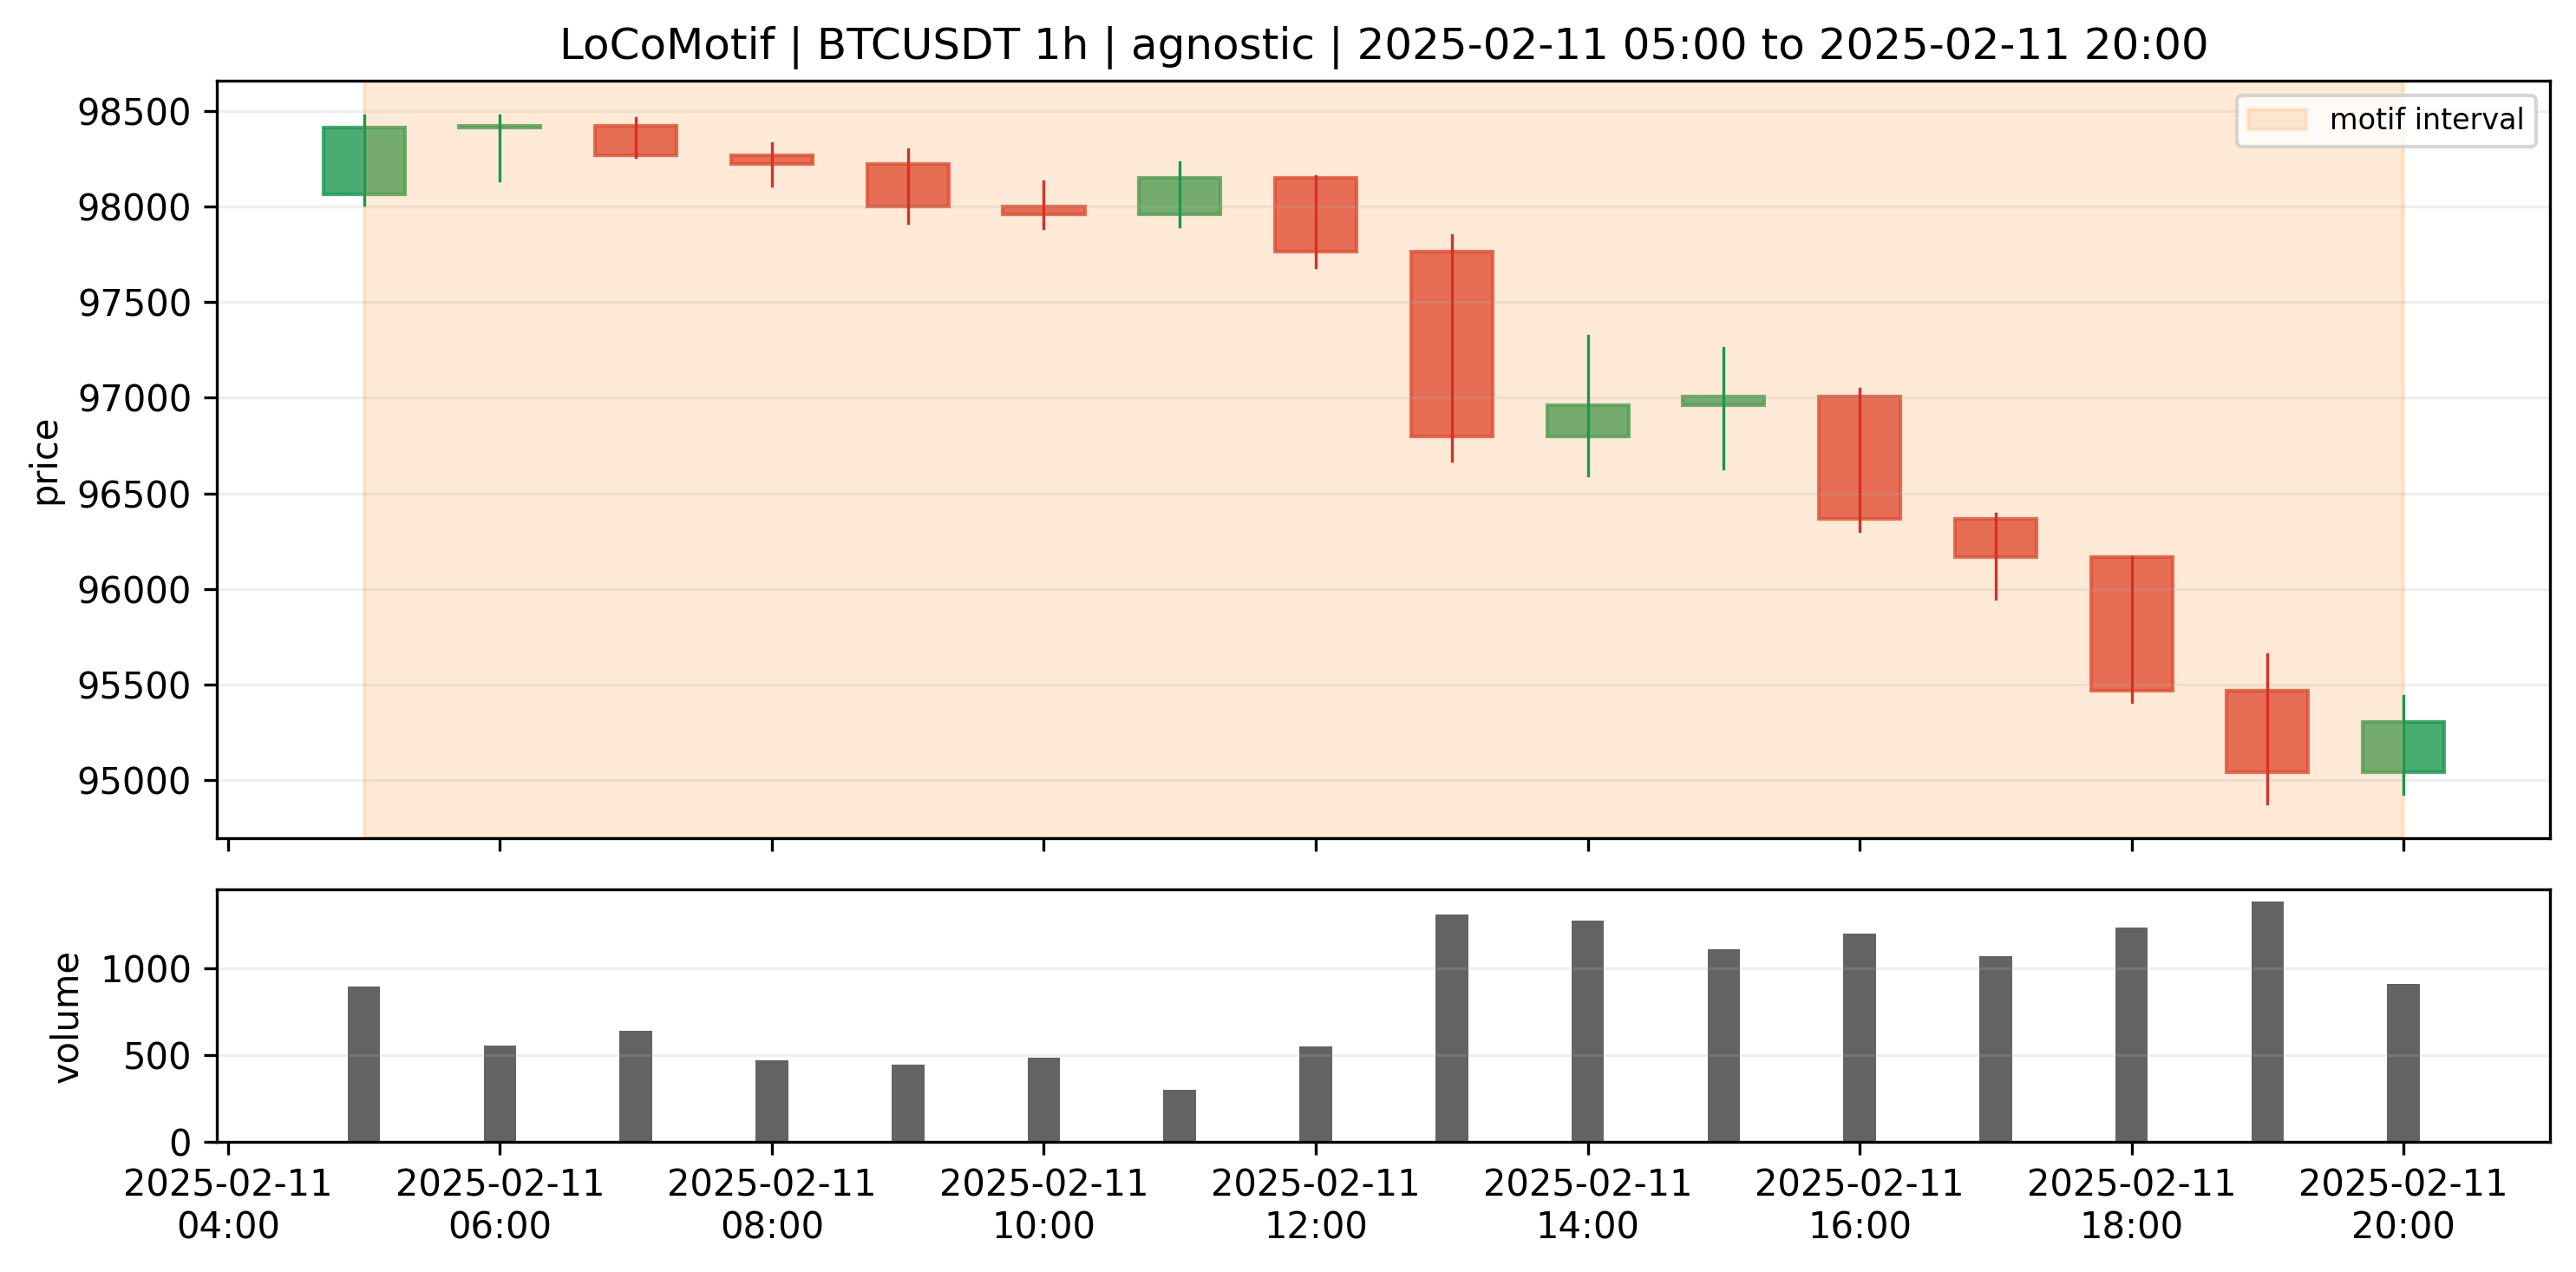
\includegraphics[width=0.9\linewidth]{reports/final_visual_evidence/figures/motif_08_locomotif_btcusdt_1h_agnostic_nan_nan_zoom.png}
\caption{motif 08 locomotif btcusdt 1h agnostic nan nan zoom. The figure compares real available Matrix Profile and LoCoMotif outputs while preserving object-type differences.}
\end{figure}

\begin{figure}[ht]
\centering
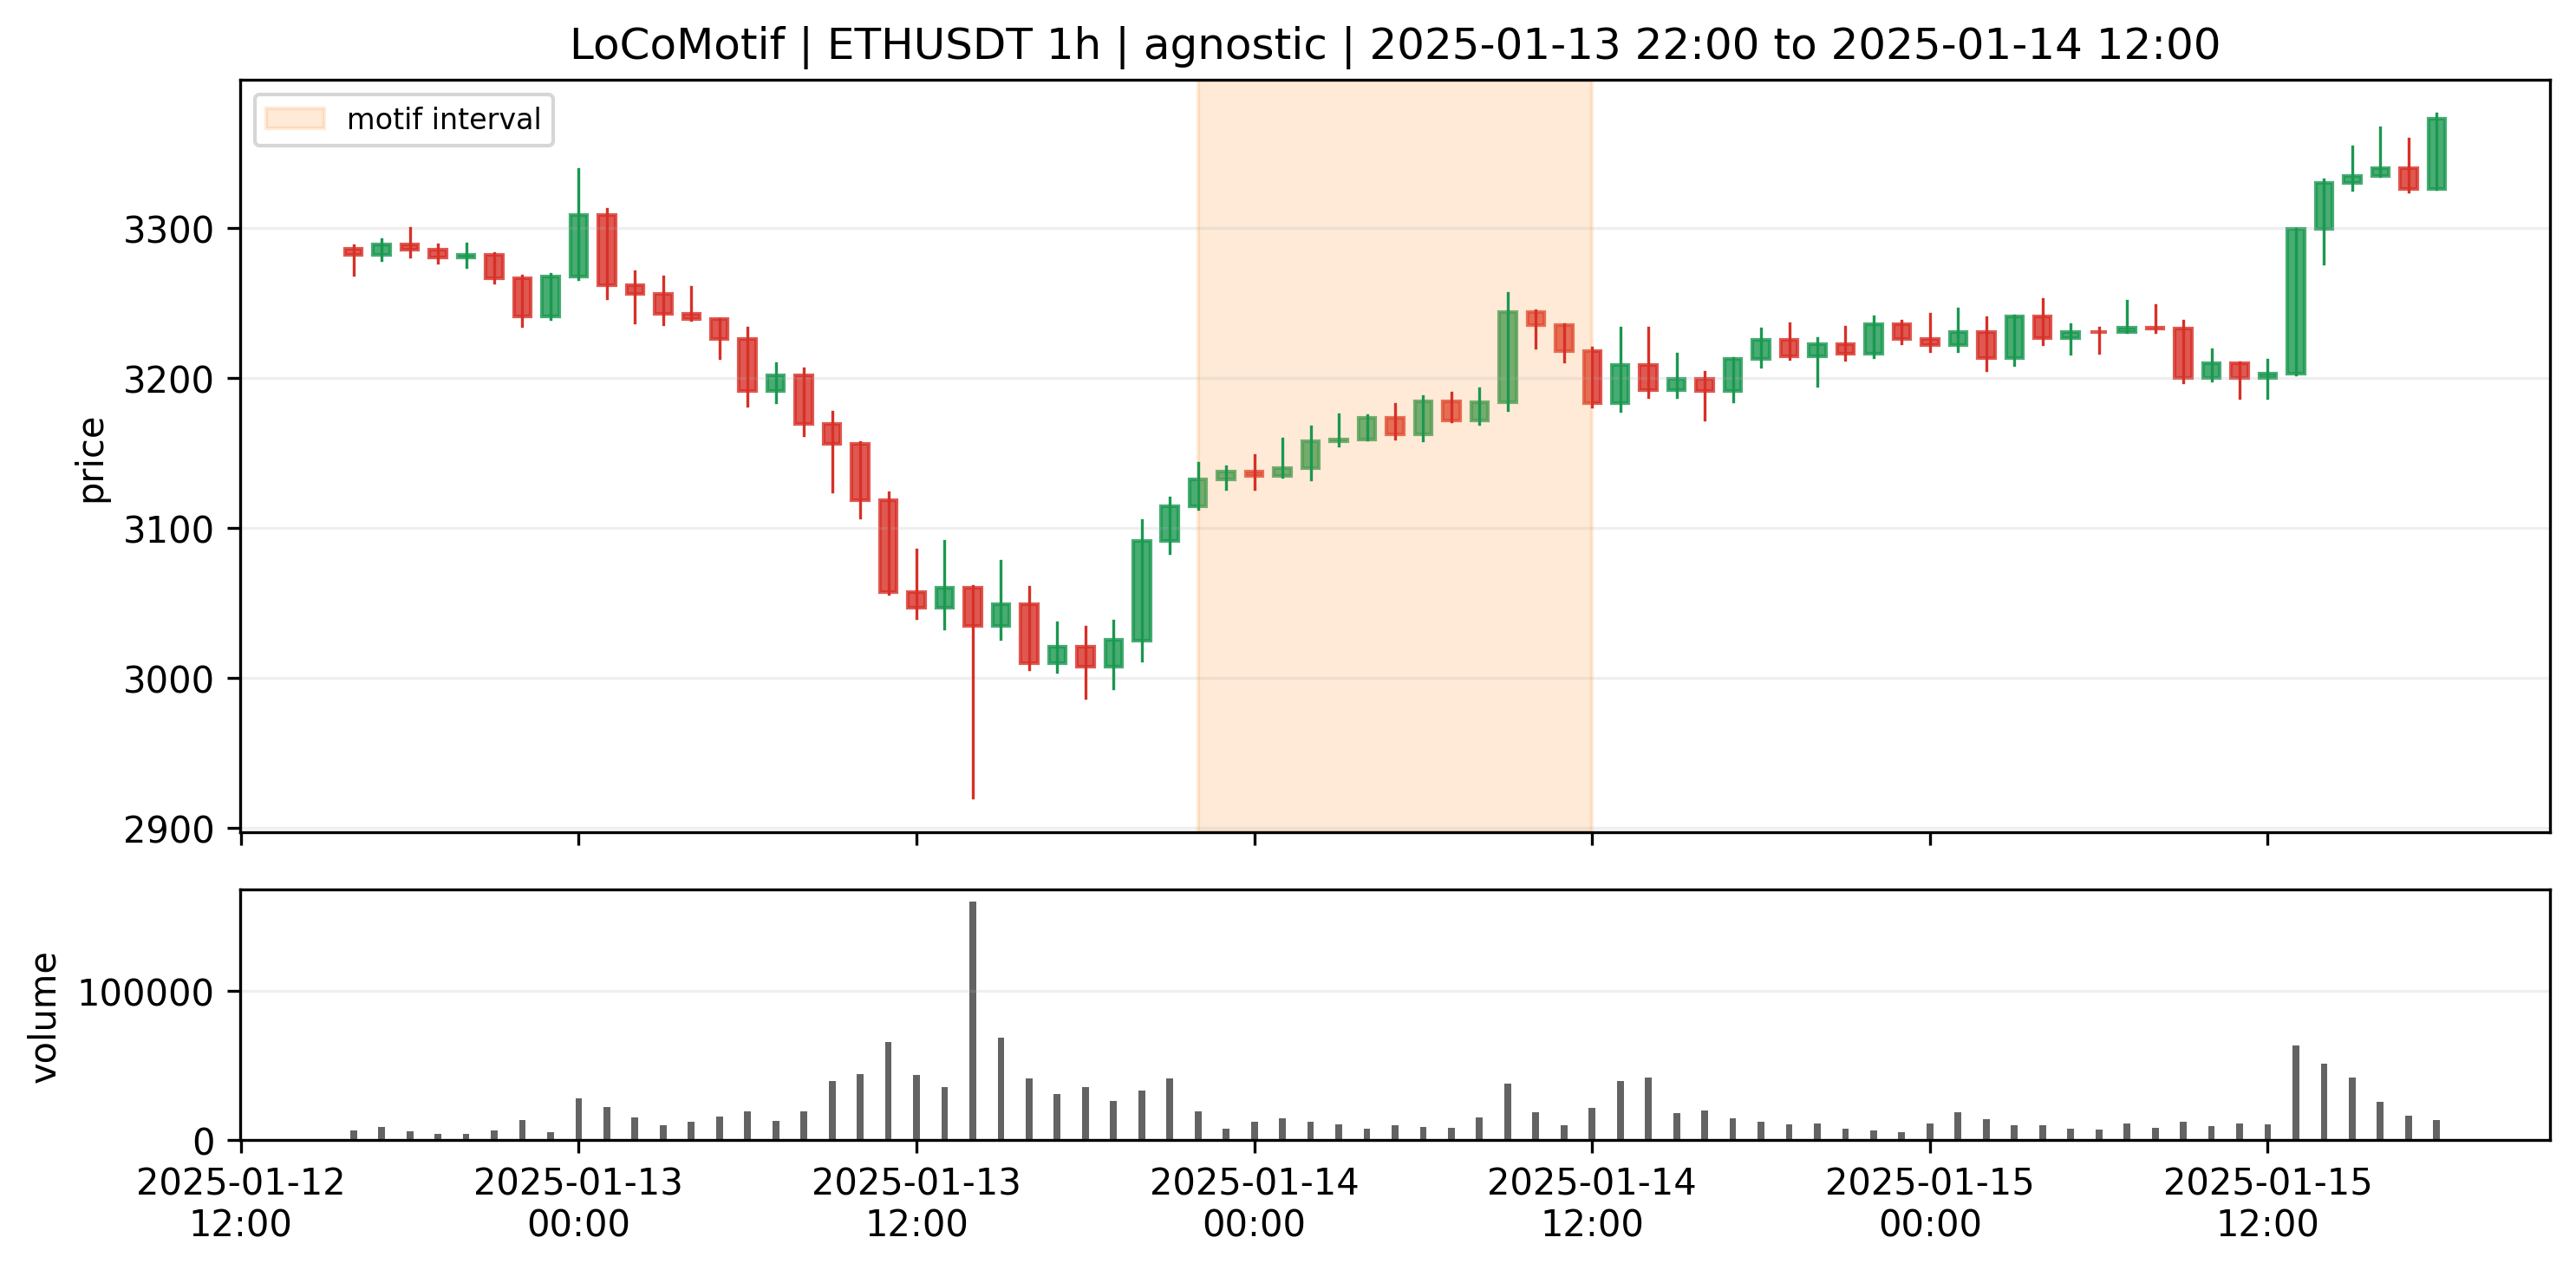
\includegraphics[width=0.9\linewidth]{reports/final_visual_evidence/figures/motif_09_locomotif_ethusdt_1h_agnostic_nan_nan_context.png}
\caption{motif 09 locomotif ethusdt 1h agnostic nan nan context. The figure compares real available Matrix Profile and LoCoMotif outputs while preserving object-type differences.}
\end{figure}

\begin{figure}[ht]
\centering
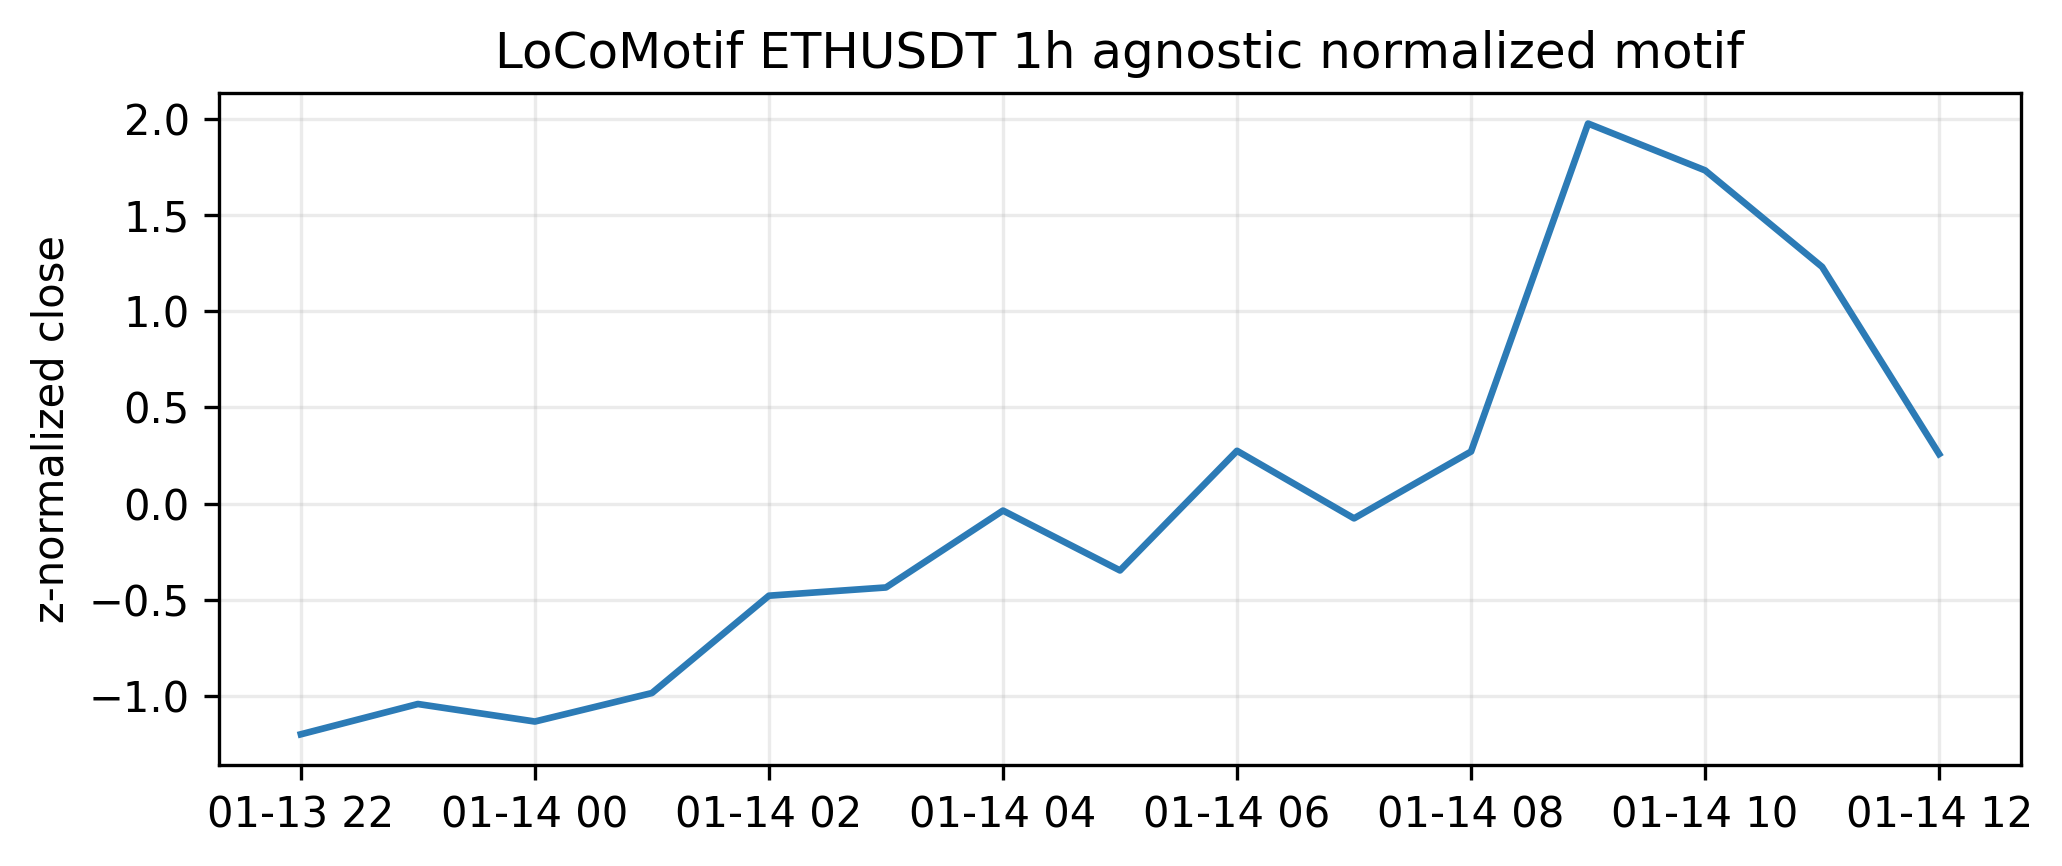
\includegraphics[width=0.9\linewidth]{reports/final_visual_evidence/figures/motif_09_locomotif_ethusdt_1h_agnostic_nan_nan_normal_pattern.png}
\caption{motif 09 locomotif ethusdt 1h agnostic nan nan normal pattern. The figure compares real available Matrix Profile and LoCoMotif outputs while preserving object-type differences.}
\end{figure}

\begin{figure}[ht]
\centering
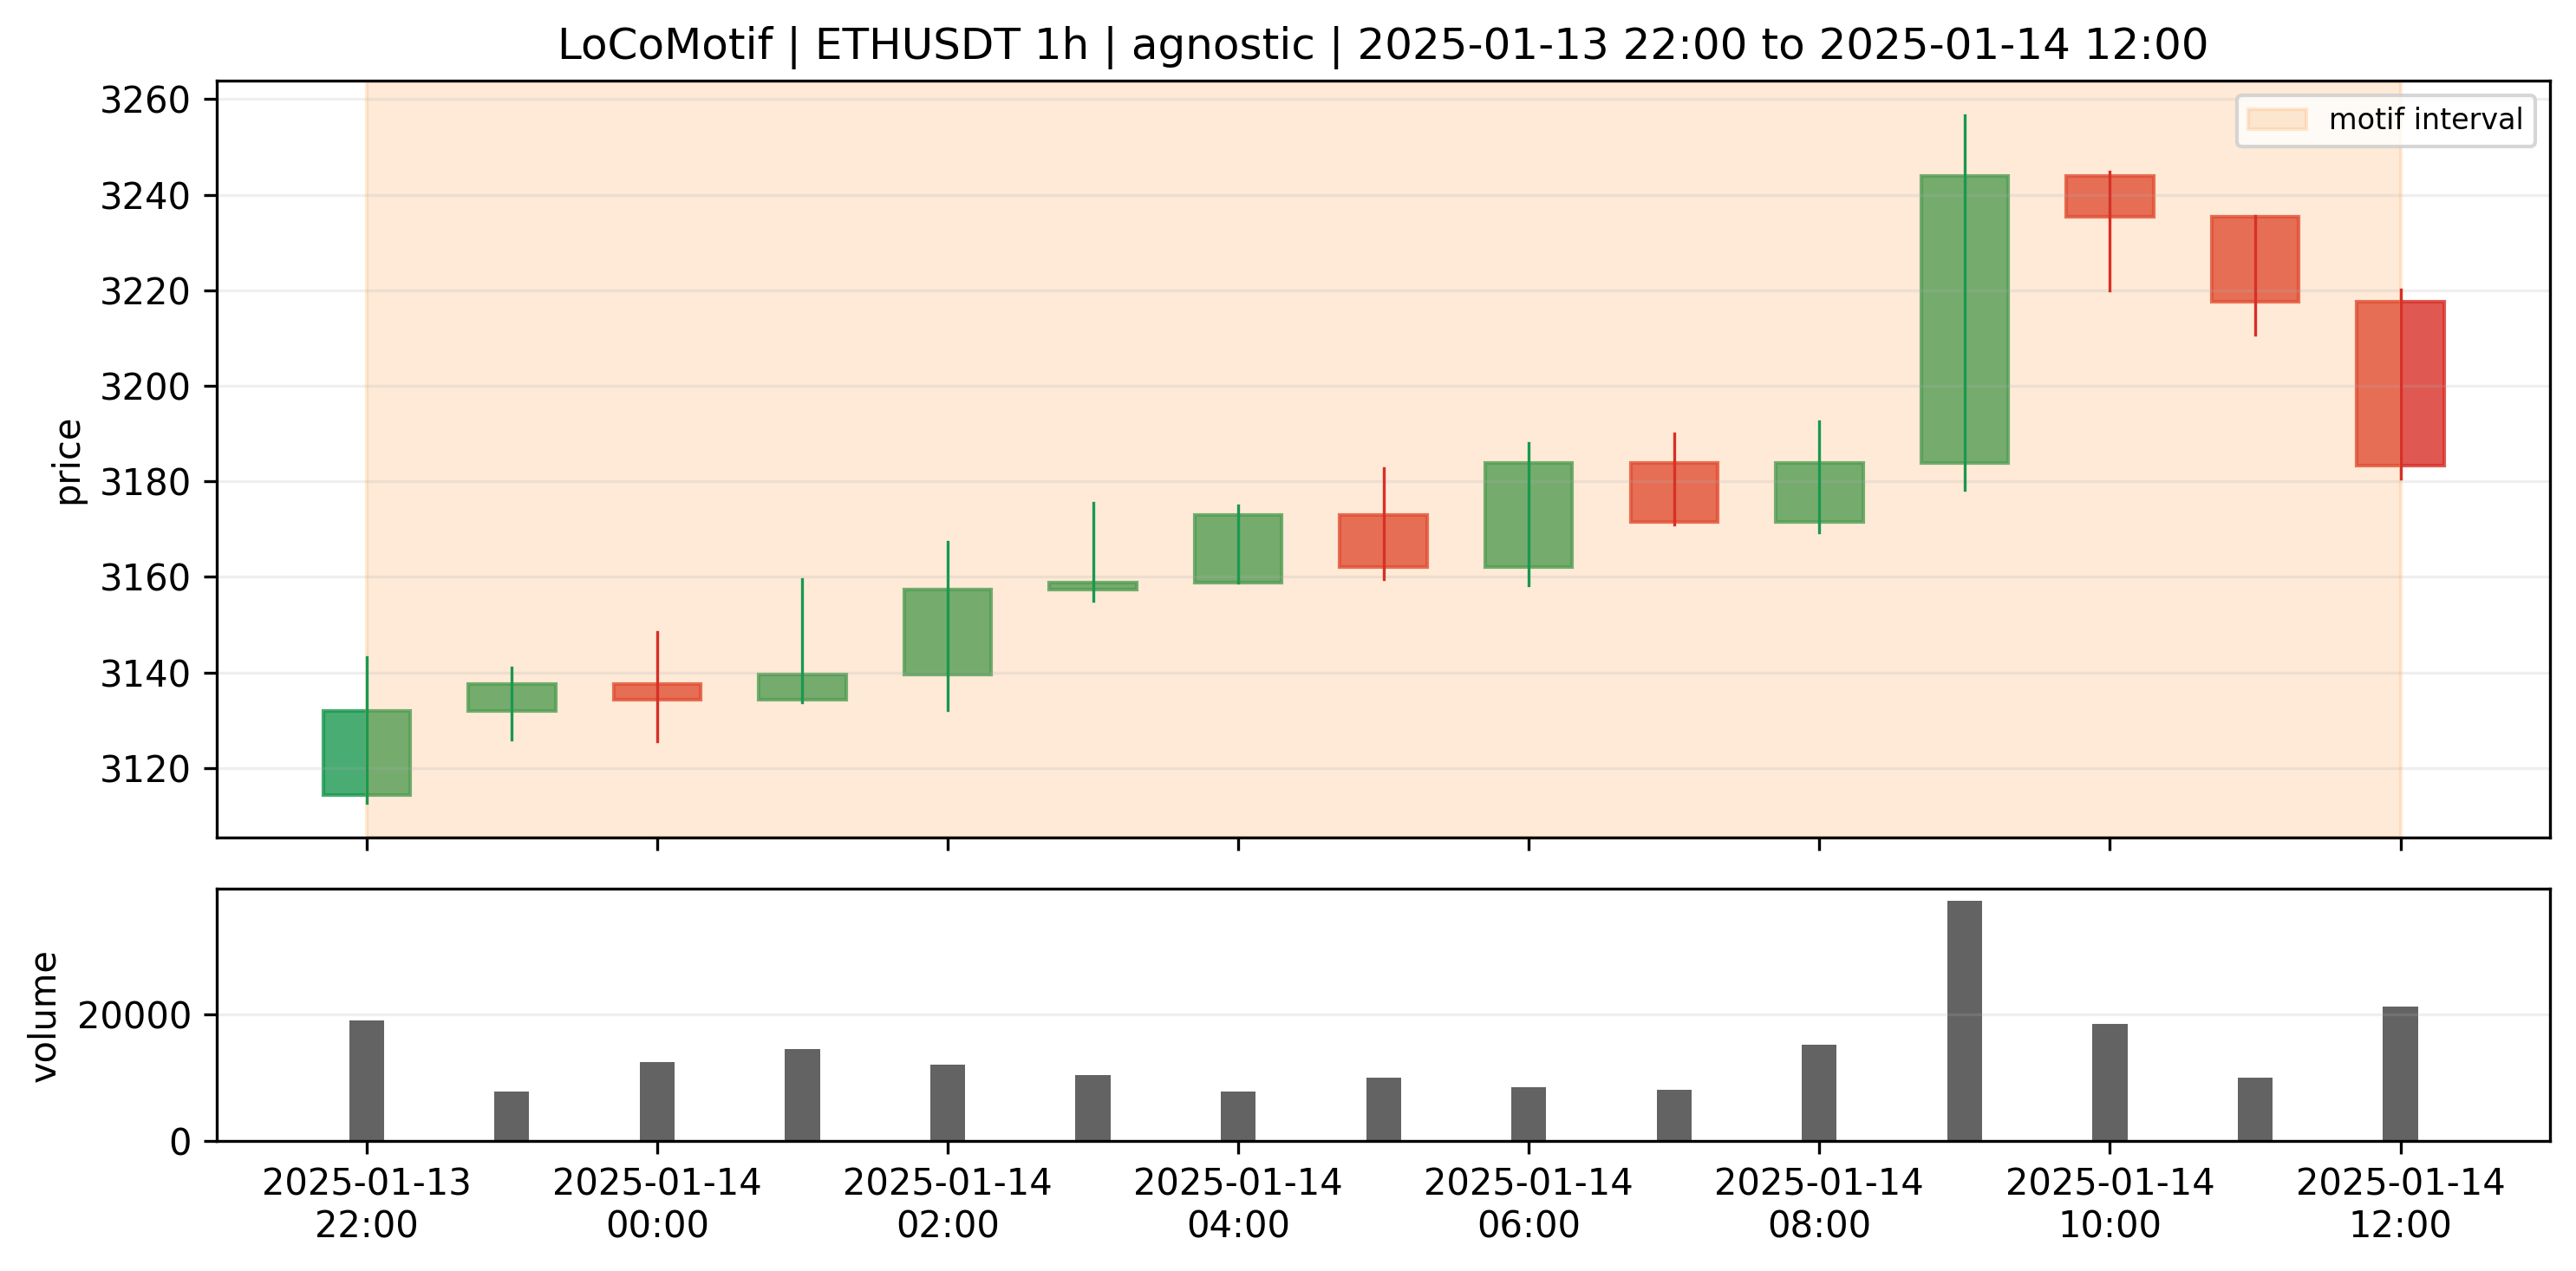
\includegraphics[width=0.9\linewidth]{reports/final_visual_evidence/figures/motif_09_locomotif_ethusdt_1h_agnostic_nan_nan_zoom.png}
\caption{motif 09 locomotif ethusdt 1h agnostic nan nan zoom. The figure compares real available Matrix Profile and LoCoMotif outputs while preserving object-type differences.}
\end{figure}

\begin{figure}[ht]
\centering
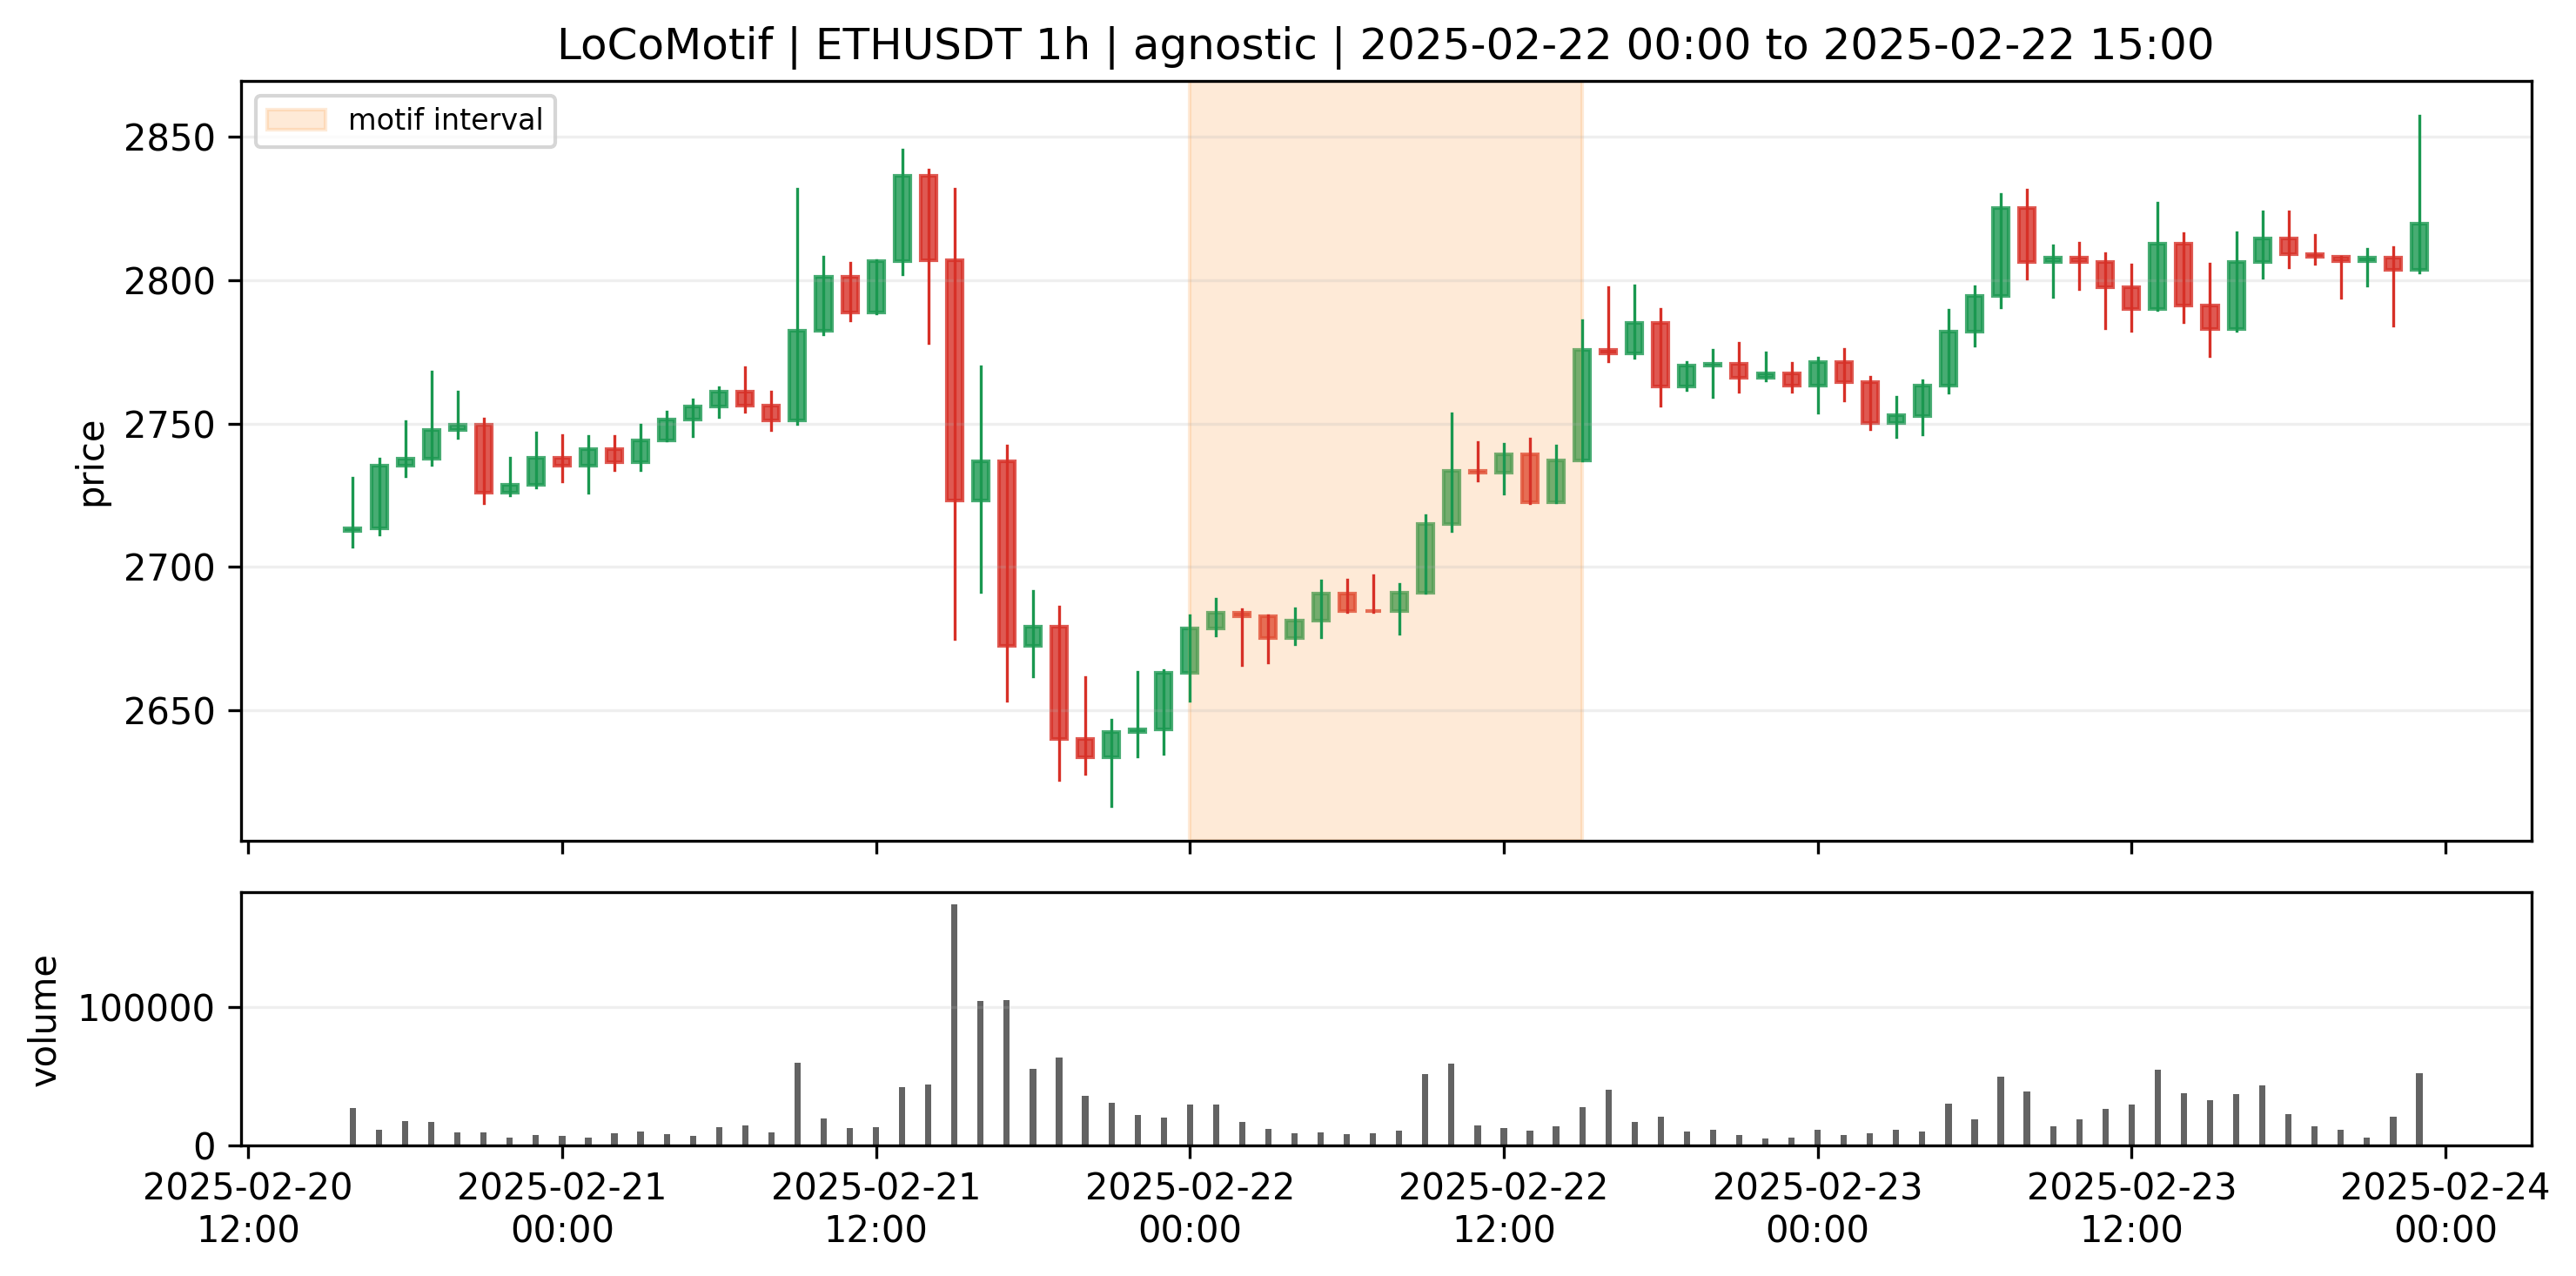
\includegraphics[width=0.9\linewidth]{reports/final_visual_evidence/figures/motif_10_locomotif_ethusdt_1h_agnostic_nan_nan_context.png}
\caption{motif 10 locomotif ethusdt 1h agnostic nan nan context. The figure compares real available Matrix Profile and LoCoMotif outputs while preserving object-type differences.}
\end{figure}

\begin{figure}[ht]
\centering
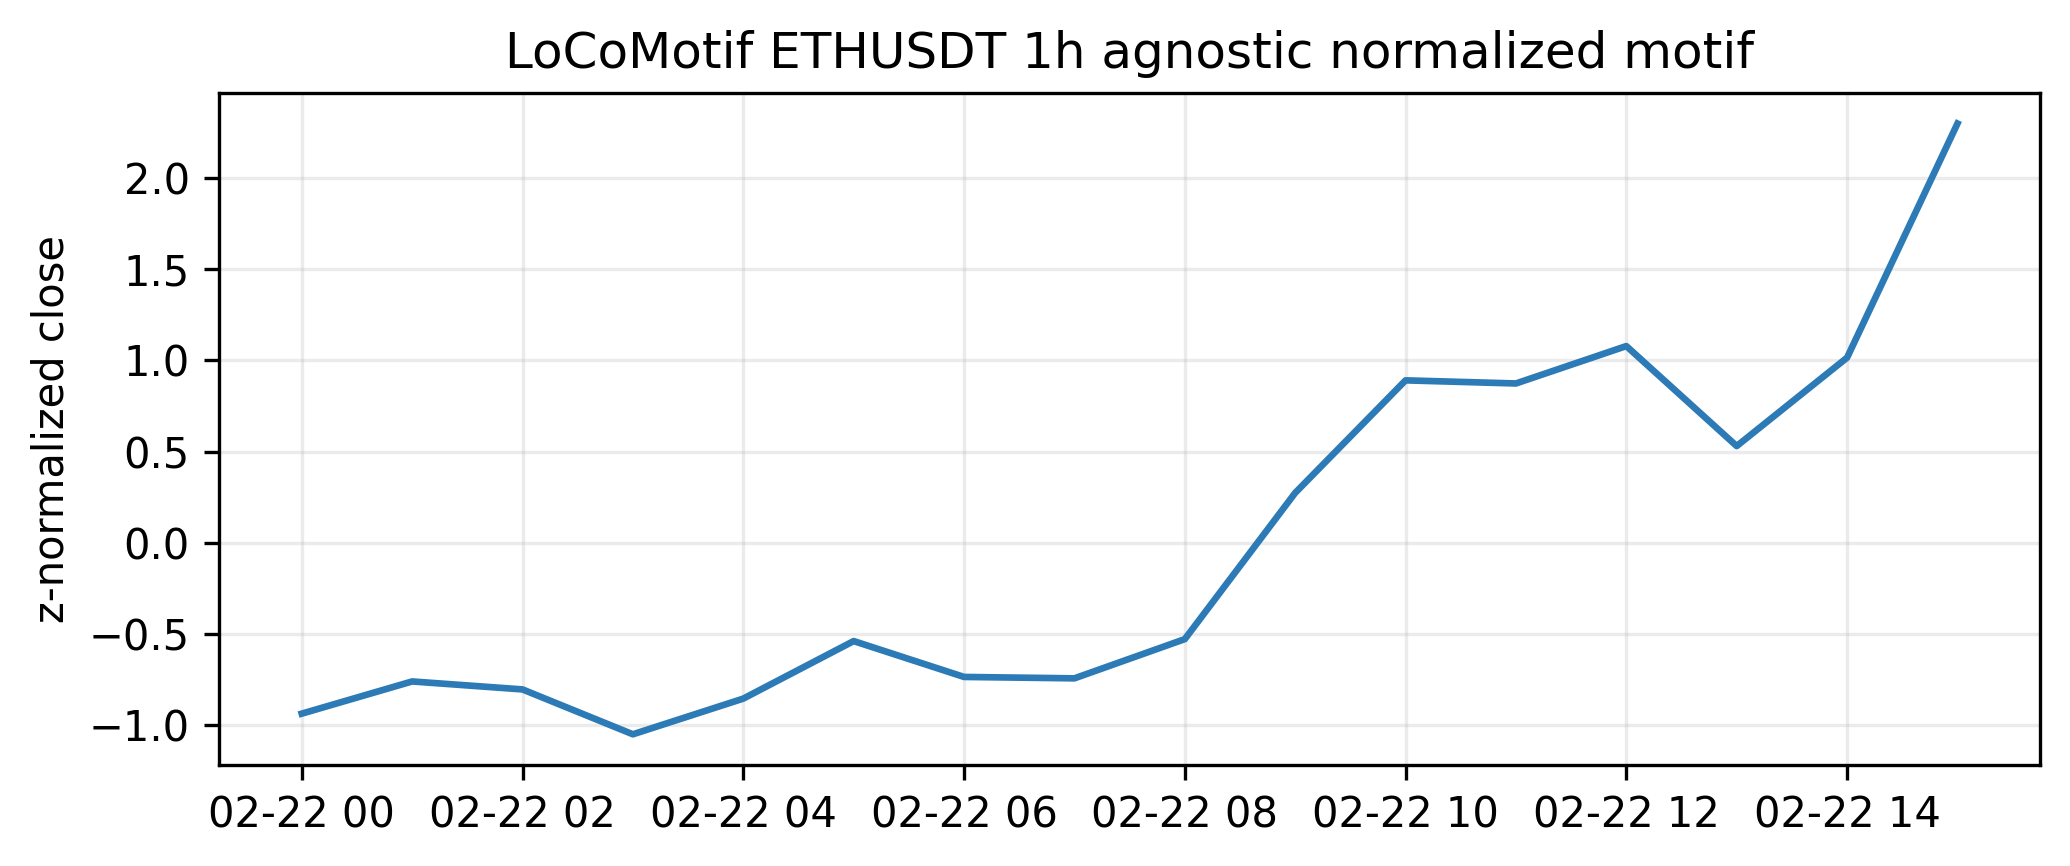
\includegraphics[width=0.9\linewidth]{reports/final_visual_evidence/figures/motif_10_locomotif_ethusdt_1h_agnostic_nan_nan_normal_pattern.png}
\caption{motif 10 locomotif ethusdt 1h agnostic nan nan normal pattern. The figure compares real available Matrix Profile and LoCoMotif outputs while preserving object-type differences.}
\end{figure}

\begin{figure}[ht]
\centering
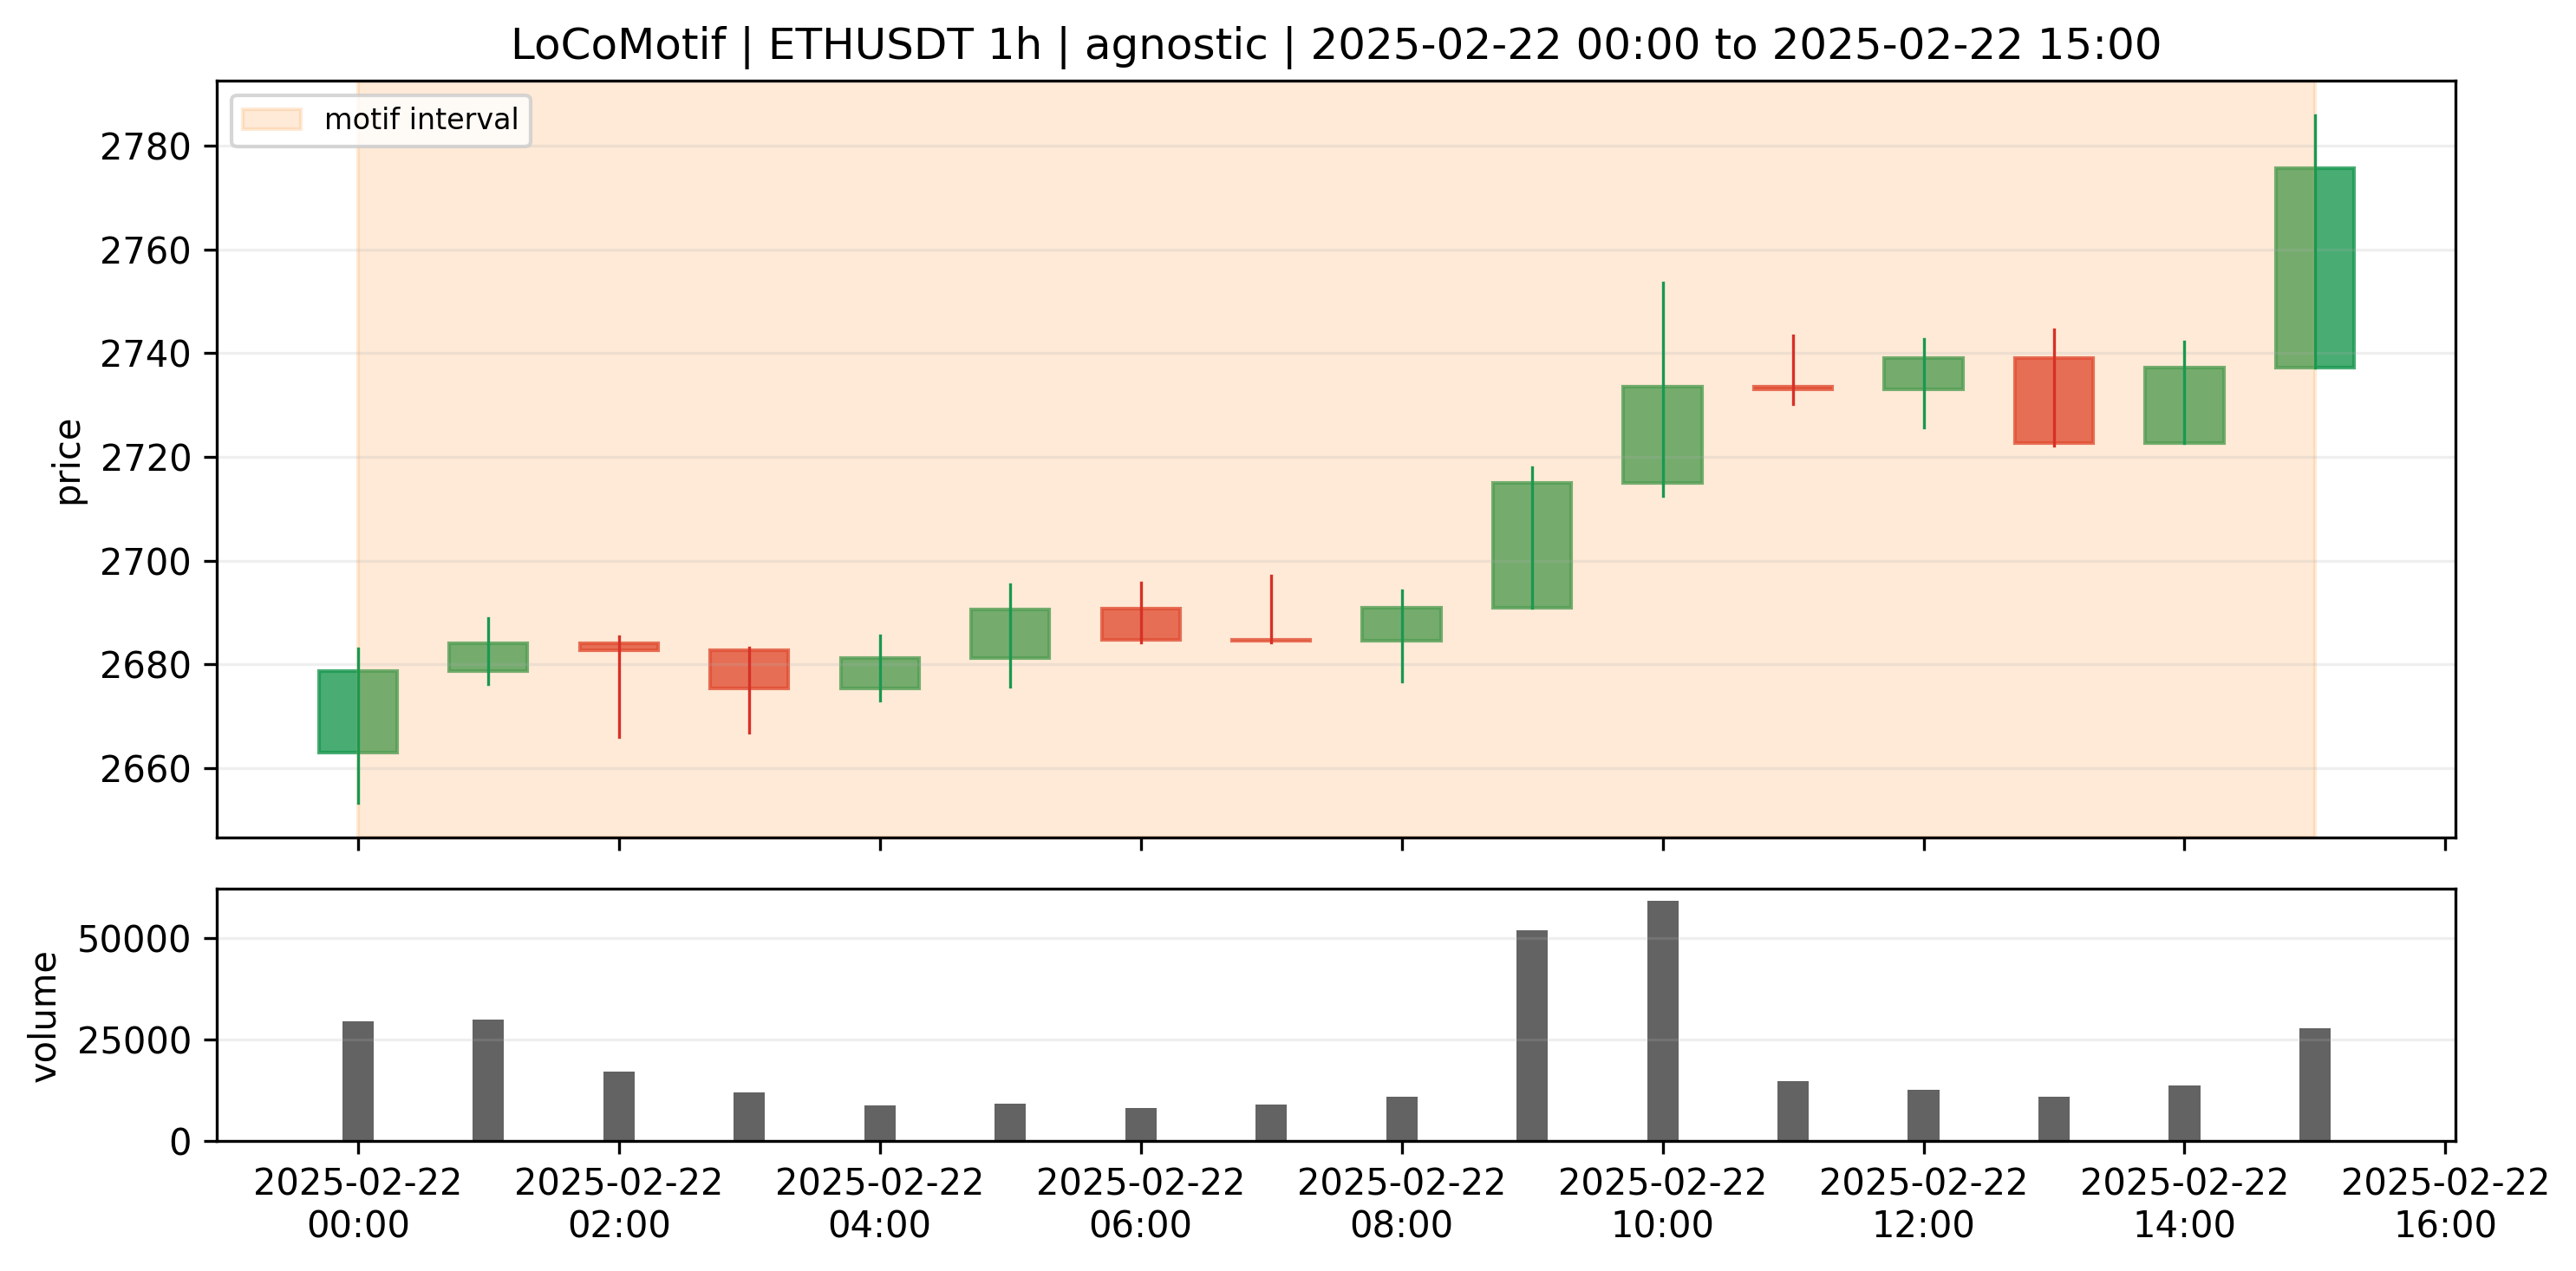
\includegraphics[width=0.9\linewidth]{reports/final_visual_evidence/figures/motif_10_locomotif_ethusdt_1h_agnostic_nan_nan_zoom.png}
\caption{motif 10 locomotif ethusdt 1h agnostic nan nan zoom. The figure compares real available Matrix Profile and LoCoMotif outputs while preserving object-type differences.}
\end{figure}

\begin{figure}[ht]
\centering
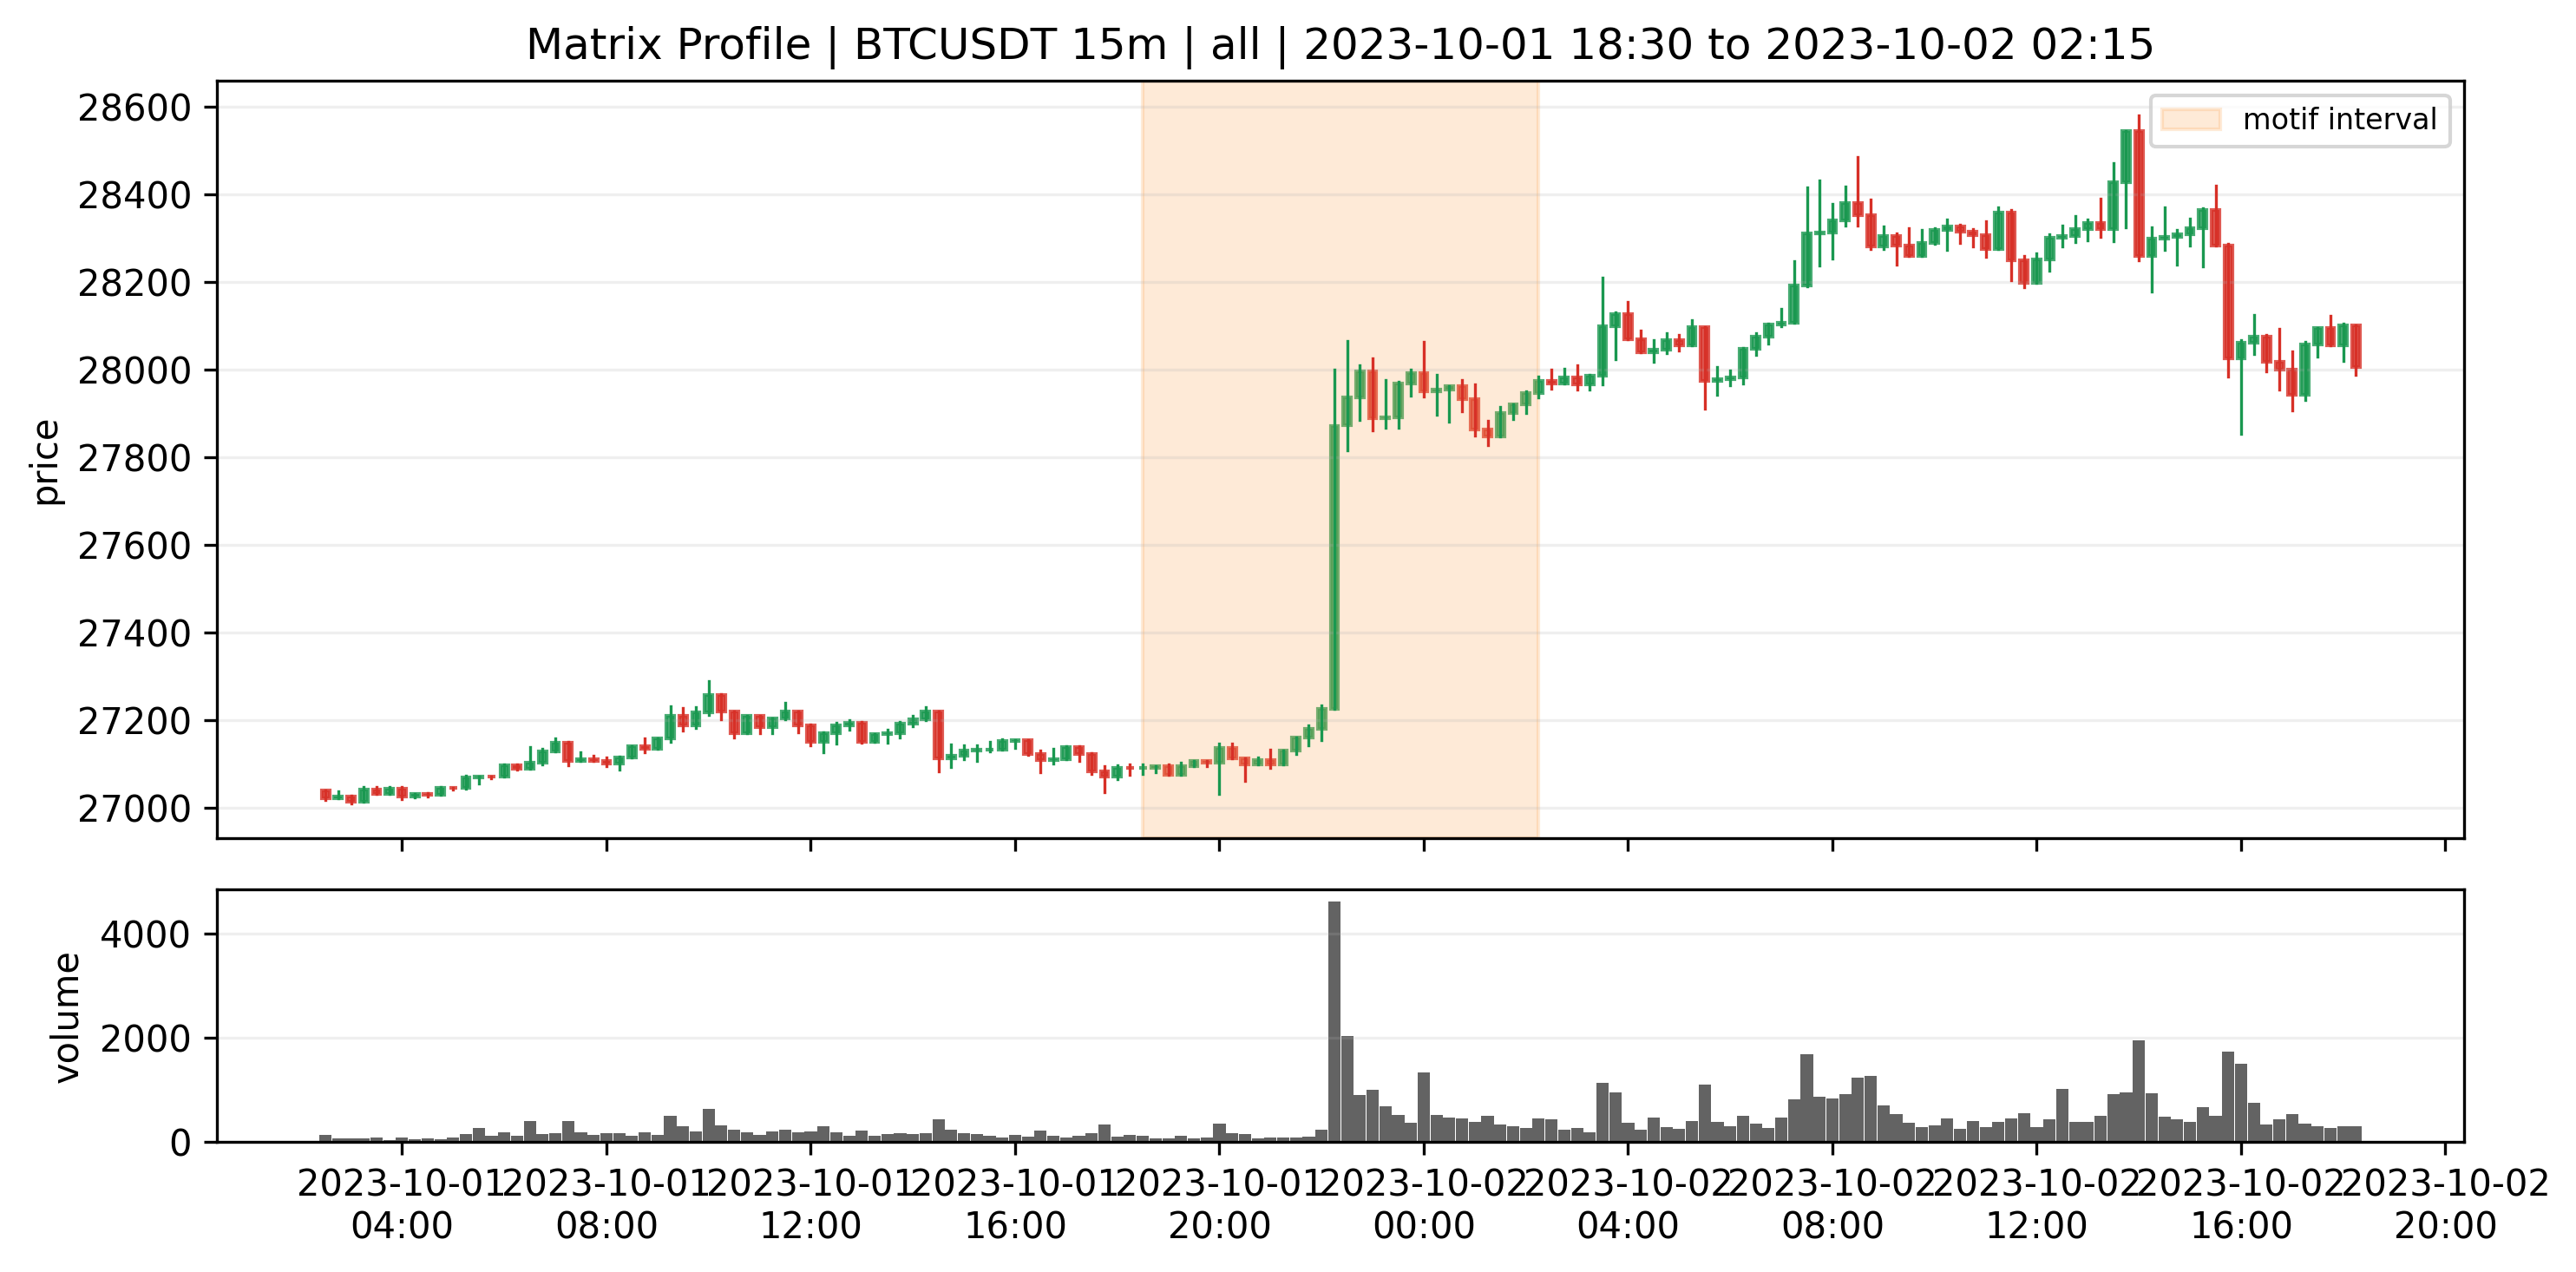
\includegraphics[width=0.9\linewidth]{reports/final_visual_evidence/figures/motif_11_matrix_profile_btcusdt_15m_all_1_0_pair21_1_context.png}
\caption{motif 11 matrix profile btcusdt 15m all 1 0 pair21 1 context. The shaded interval marks the discovered motif occurrence in original price context.}
\end{figure}

\begin{figure}[ht]
\centering
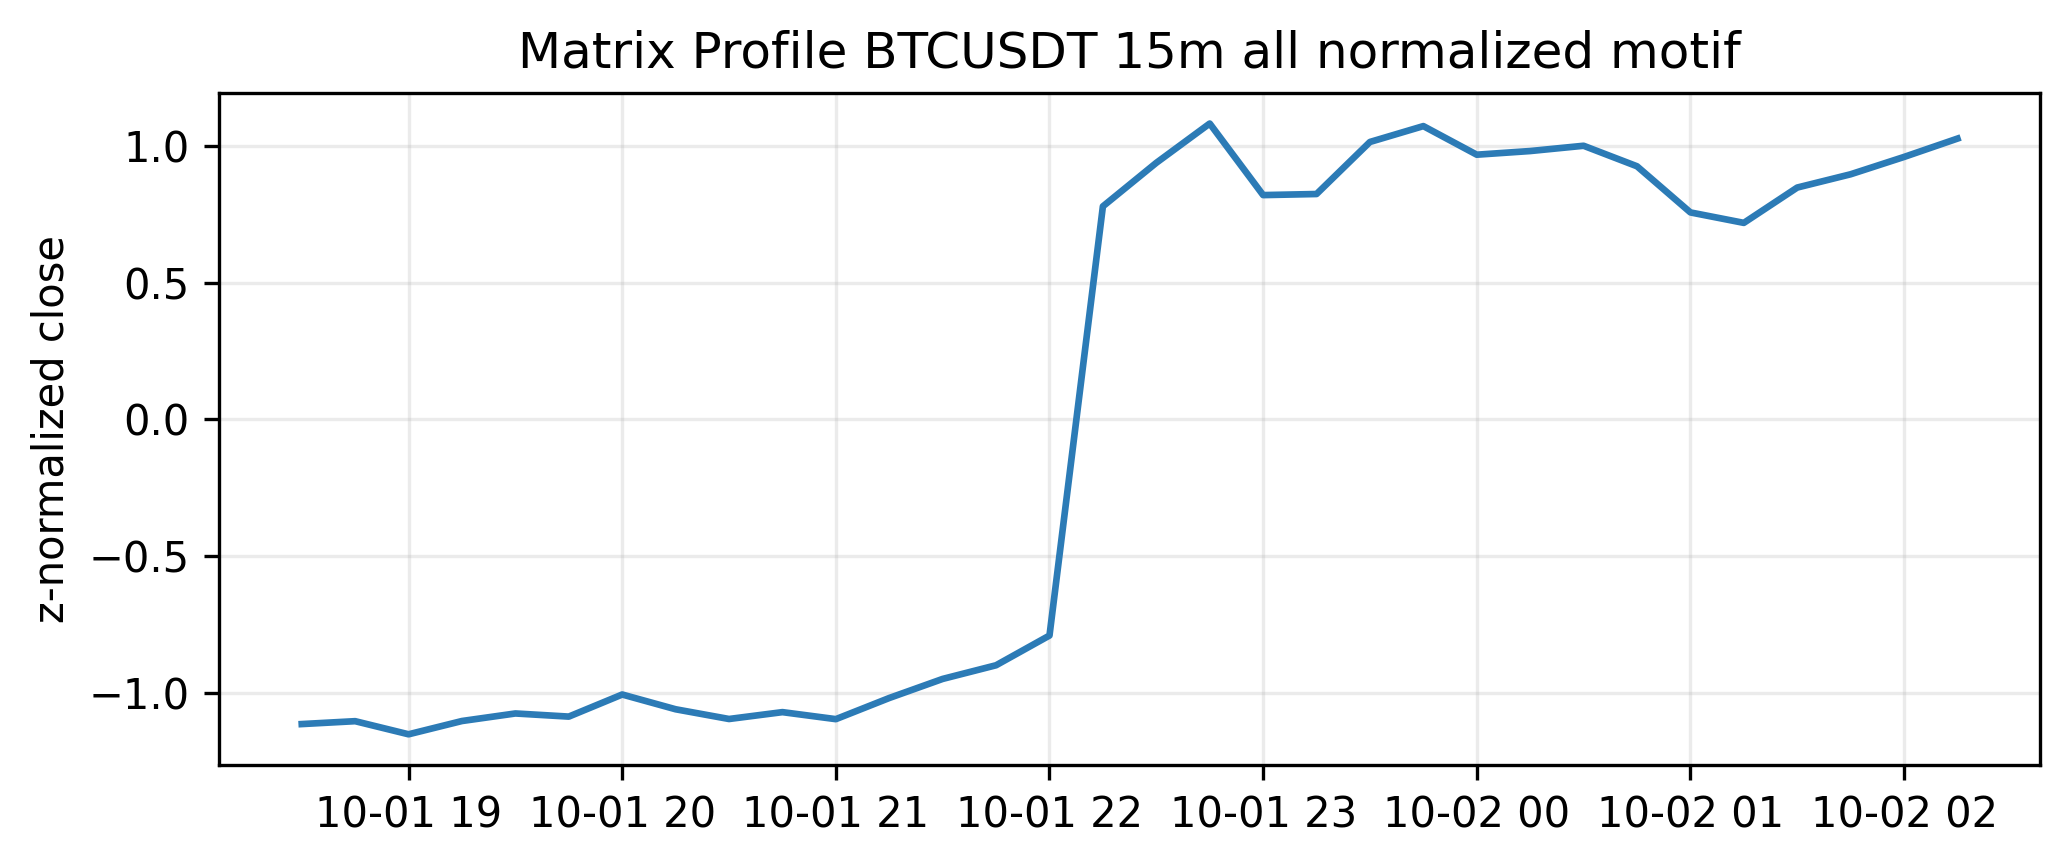
\includegraphics[width=0.9\linewidth]{reports/final_visual_evidence/figures/motif_11_matrix_profile_btcusdt_15m_all_1_0_pair21_1_normal_pattern.png}
\caption{motif 11 matrix profile btcusdt 15m all 1 0 pair21 1 normal pattern. The shaded interval marks the discovered motif occurrence in original price context.}
\end{figure}

\begin{figure}[ht]
\centering
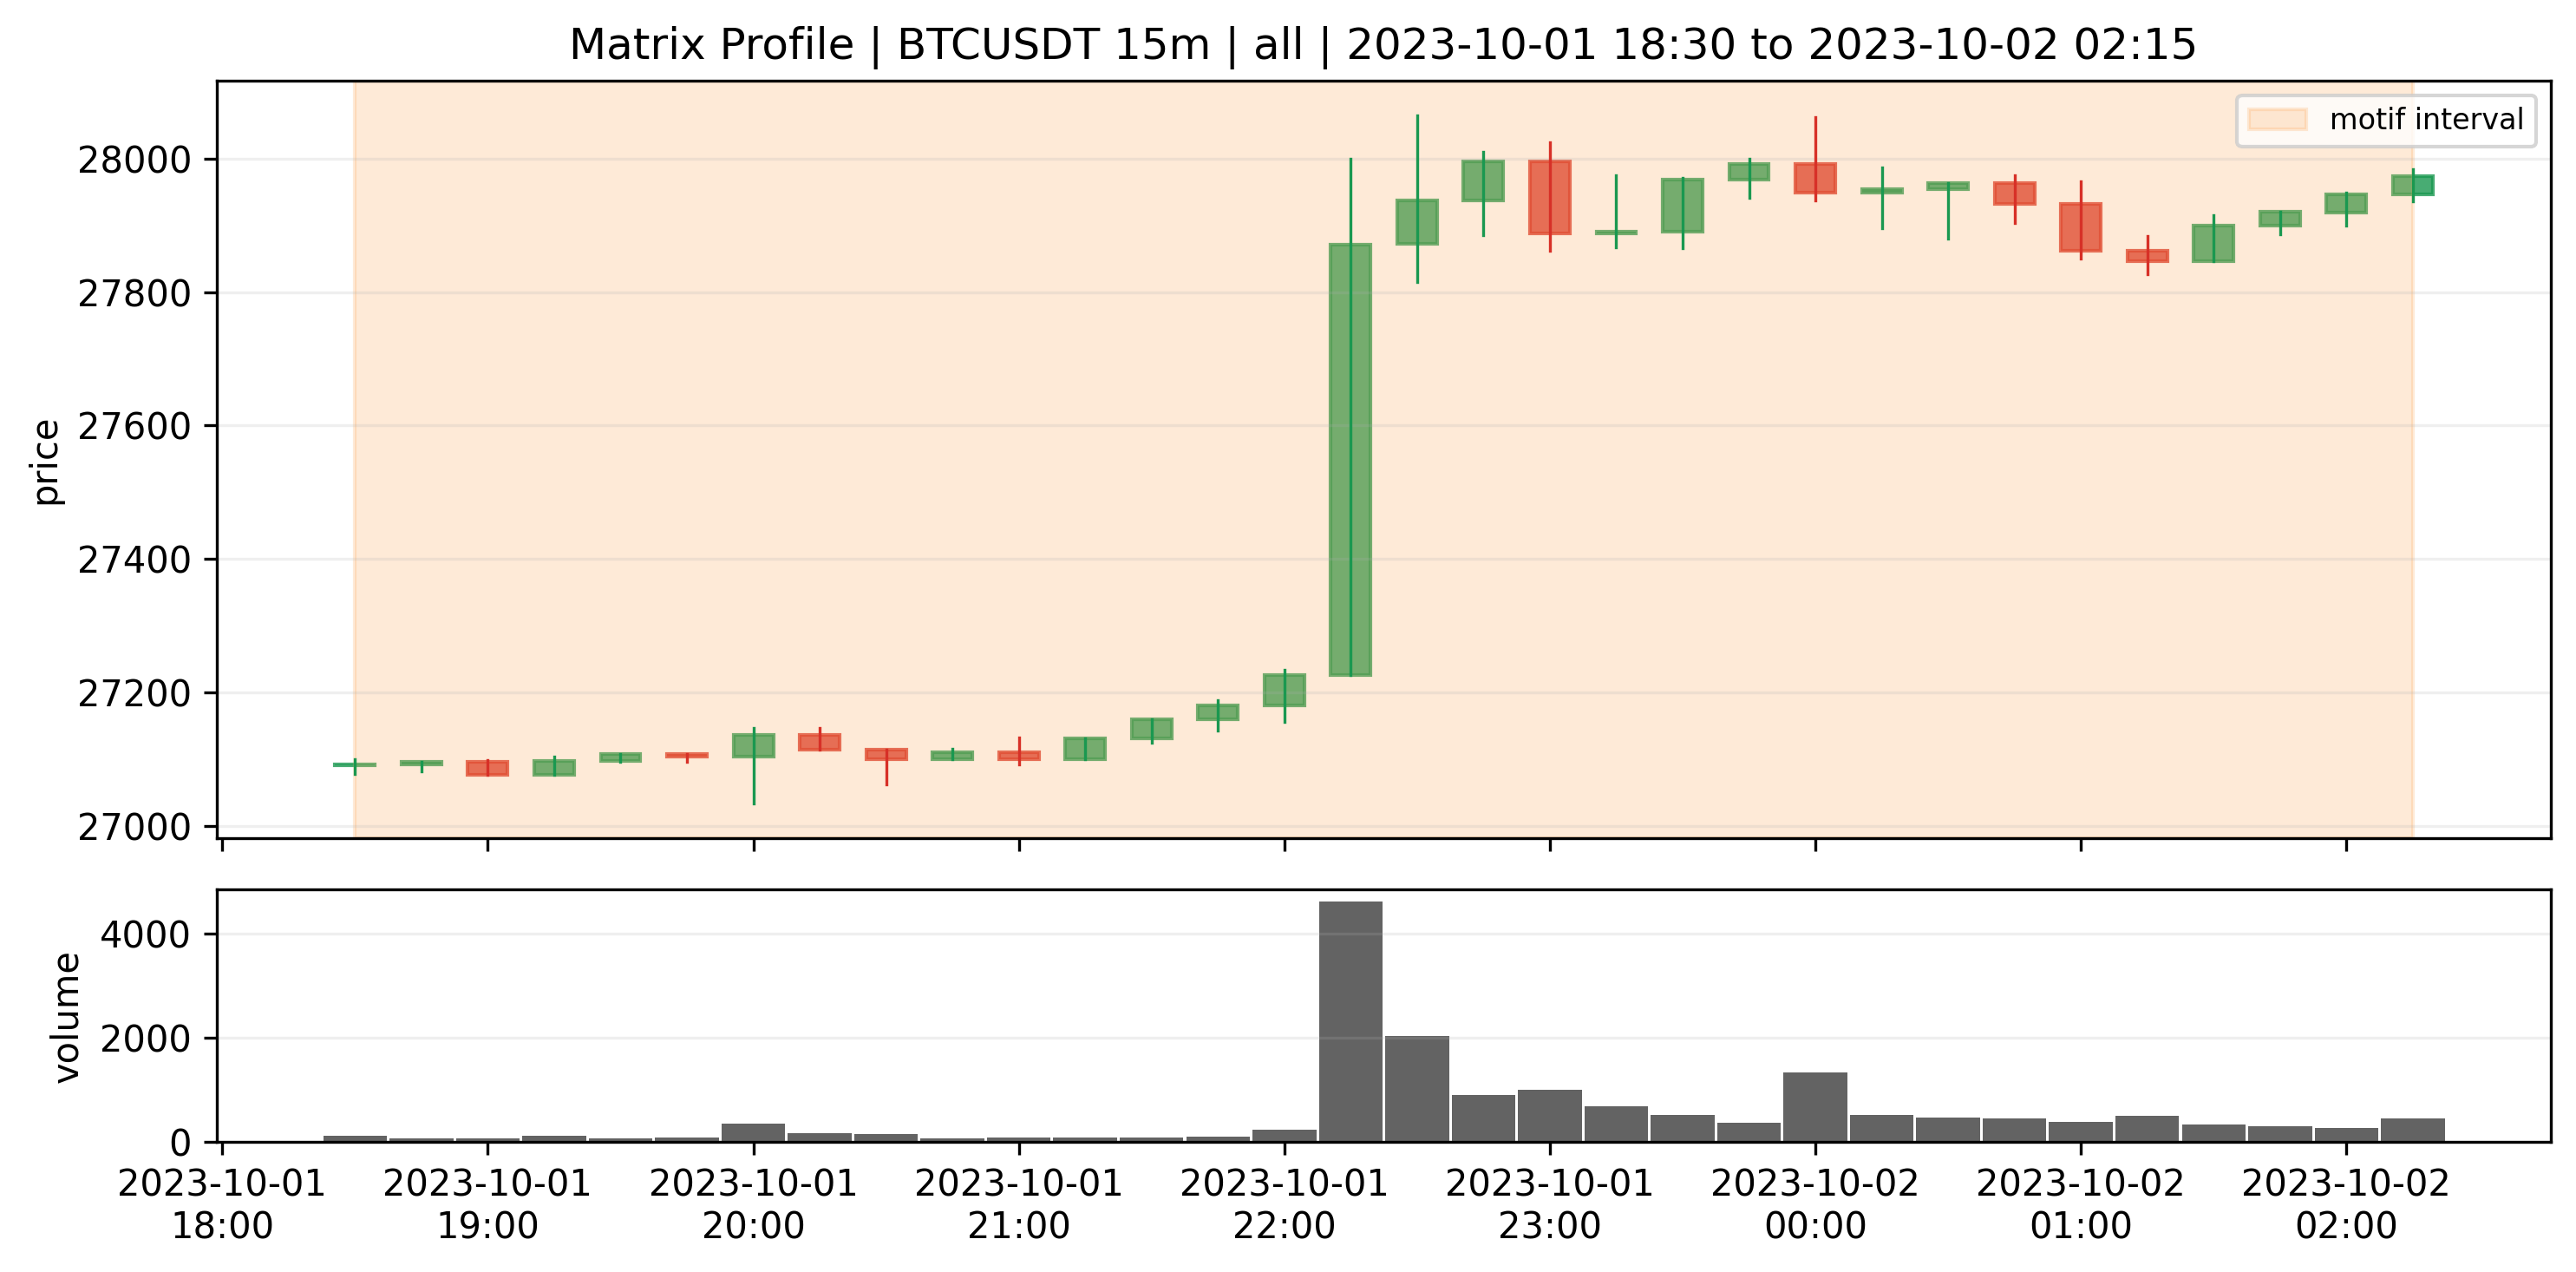
\includegraphics[width=0.9\linewidth]{reports/final_visual_evidence/figures/motif_11_matrix_profile_btcusdt_15m_all_1_0_pair21_1_zoom.png}
\caption{motif 11 matrix profile btcusdt 15m all 1 0 pair21 1 zoom. The shaded interval marks the discovered motif occurrence in original price context.}
\end{figure}

\begin{figure}[ht]
\centering
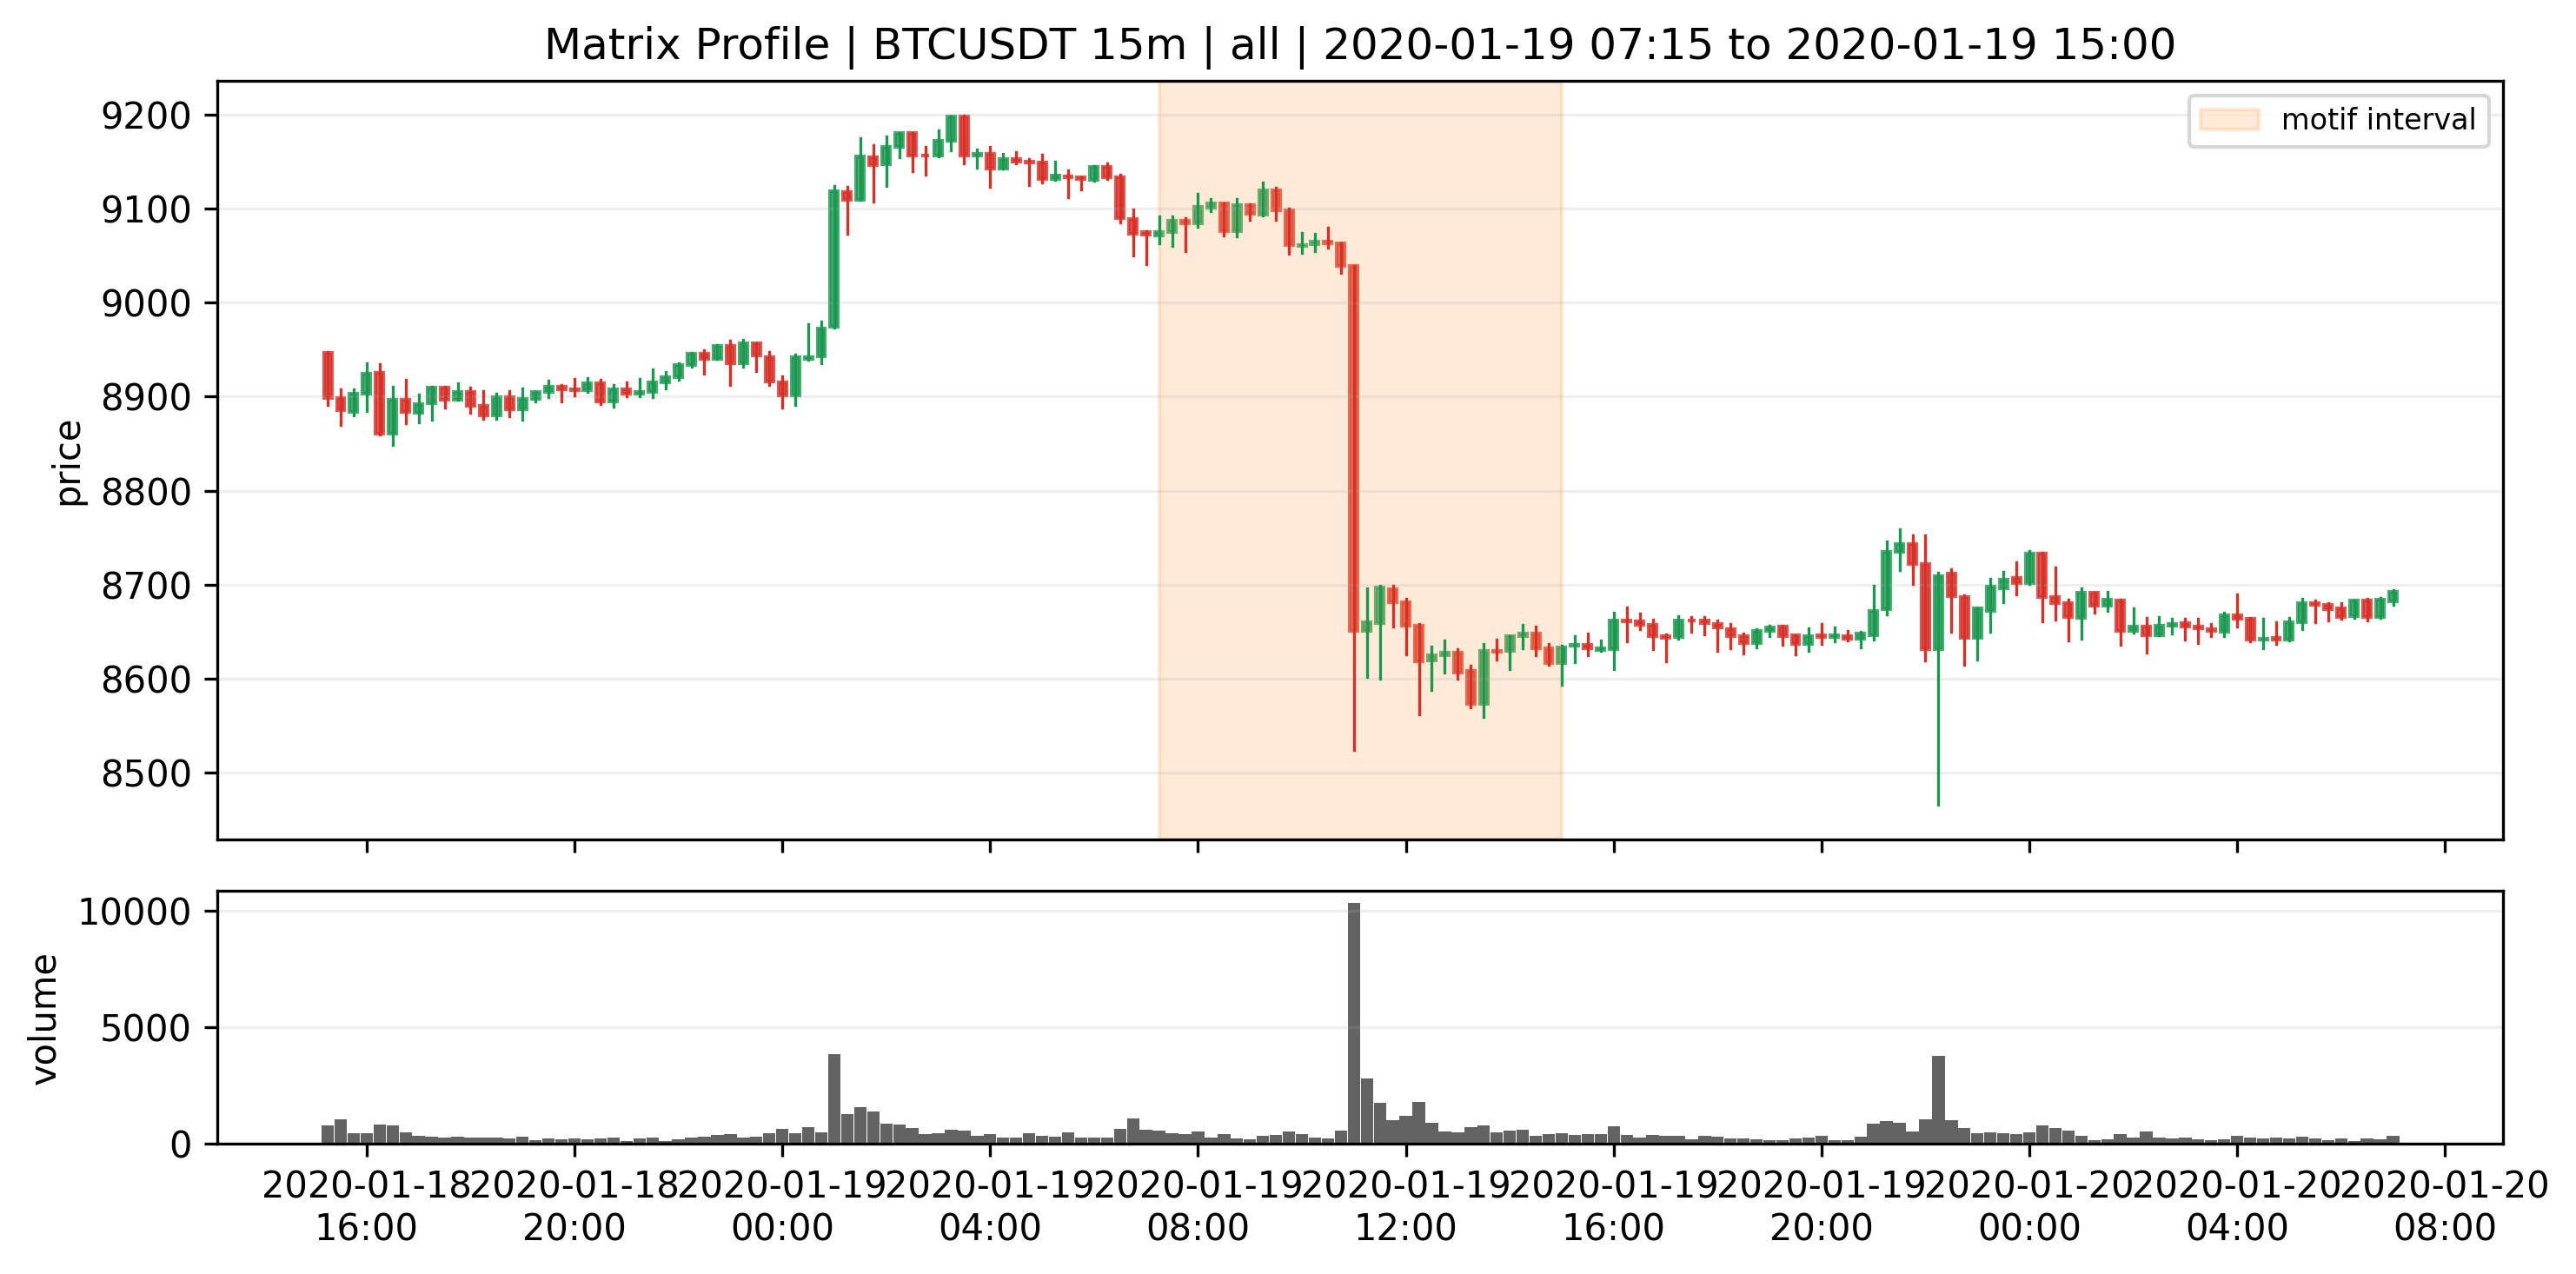
\includegraphics[width=0.9\linewidth]{reports/final_visual_evidence/figures/motif_12_matrix_profile_btcusdt_15m_all_1_0_pair21_2_context.png}
\caption{motif 12 matrix profile btcusdt 15m all 1 0 pair21 2 context. The shaded interval marks the discovered motif occurrence in original price context.}
\end{figure}

\begin{figure}[ht]
\centering
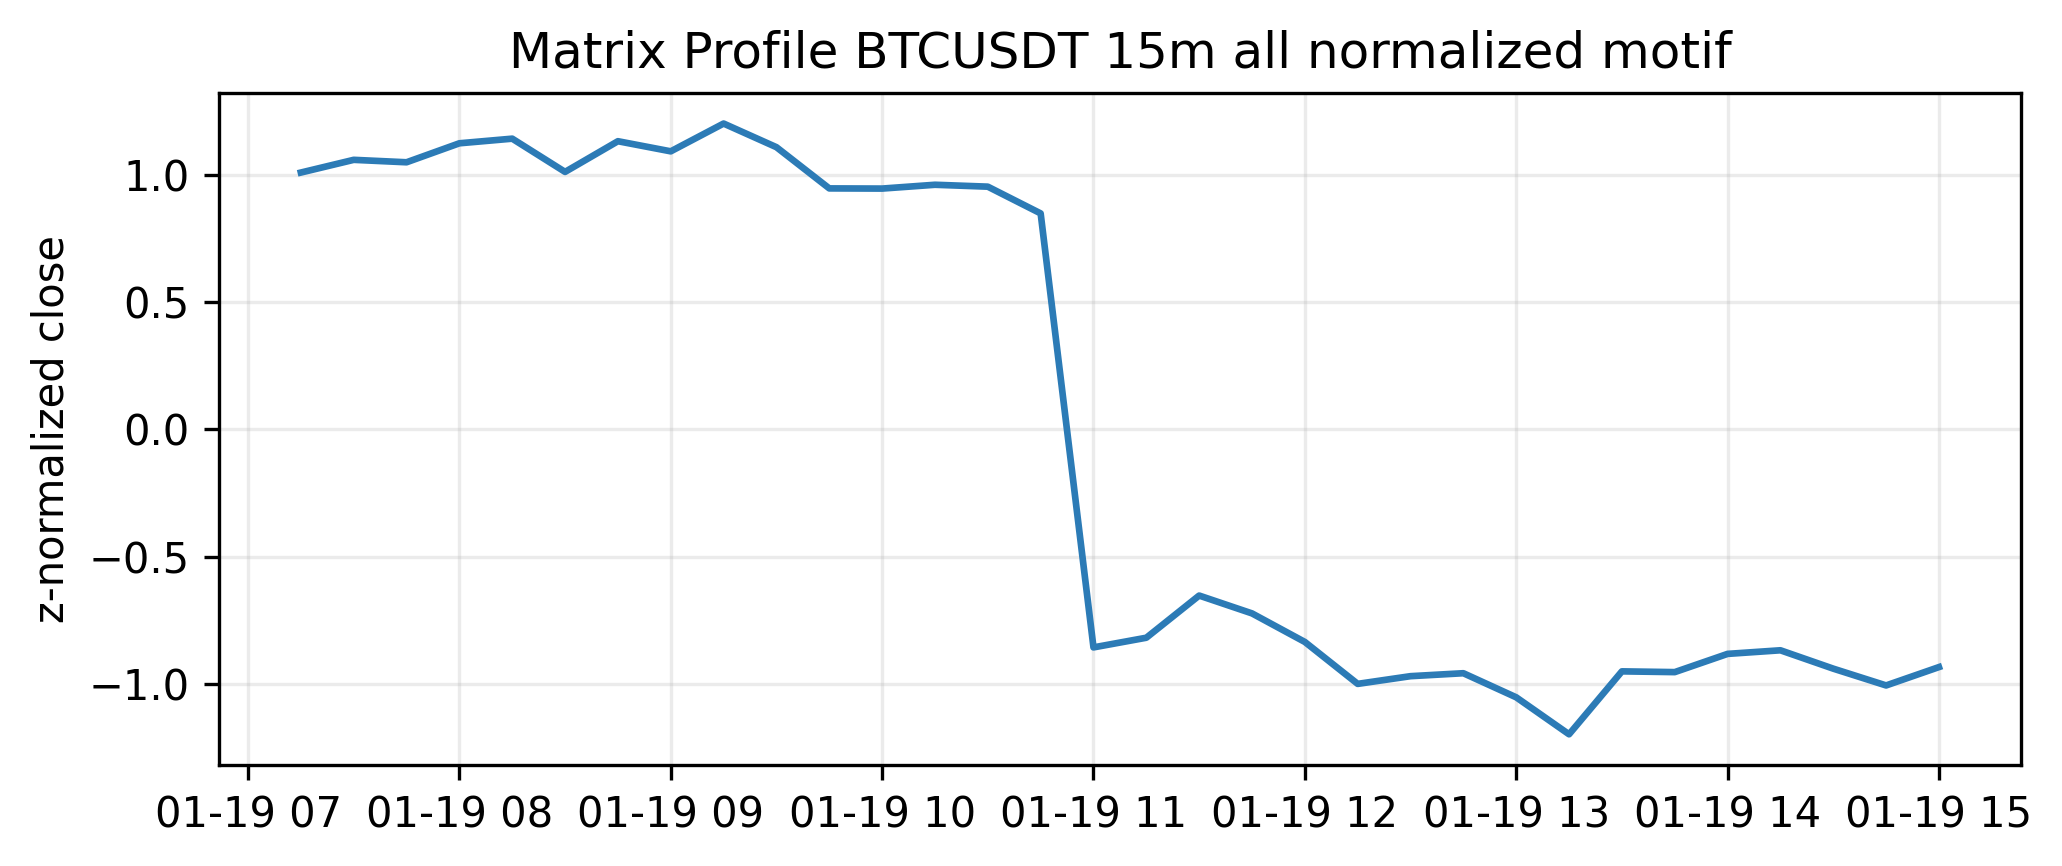
\includegraphics[width=0.9\linewidth]{reports/final_visual_evidence/figures/motif_12_matrix_profile_btcusdt_15m_all_1_0_pair21_2_normal_pattern.png}
\caption{motif 12 matrix profile btcusdt 15m all 1 0 pair21 2 normal pattern. The shaded interval marks the discovered motif occurrence in original price context.}
\end{figure}

\begin{figure}[ht]
\centering
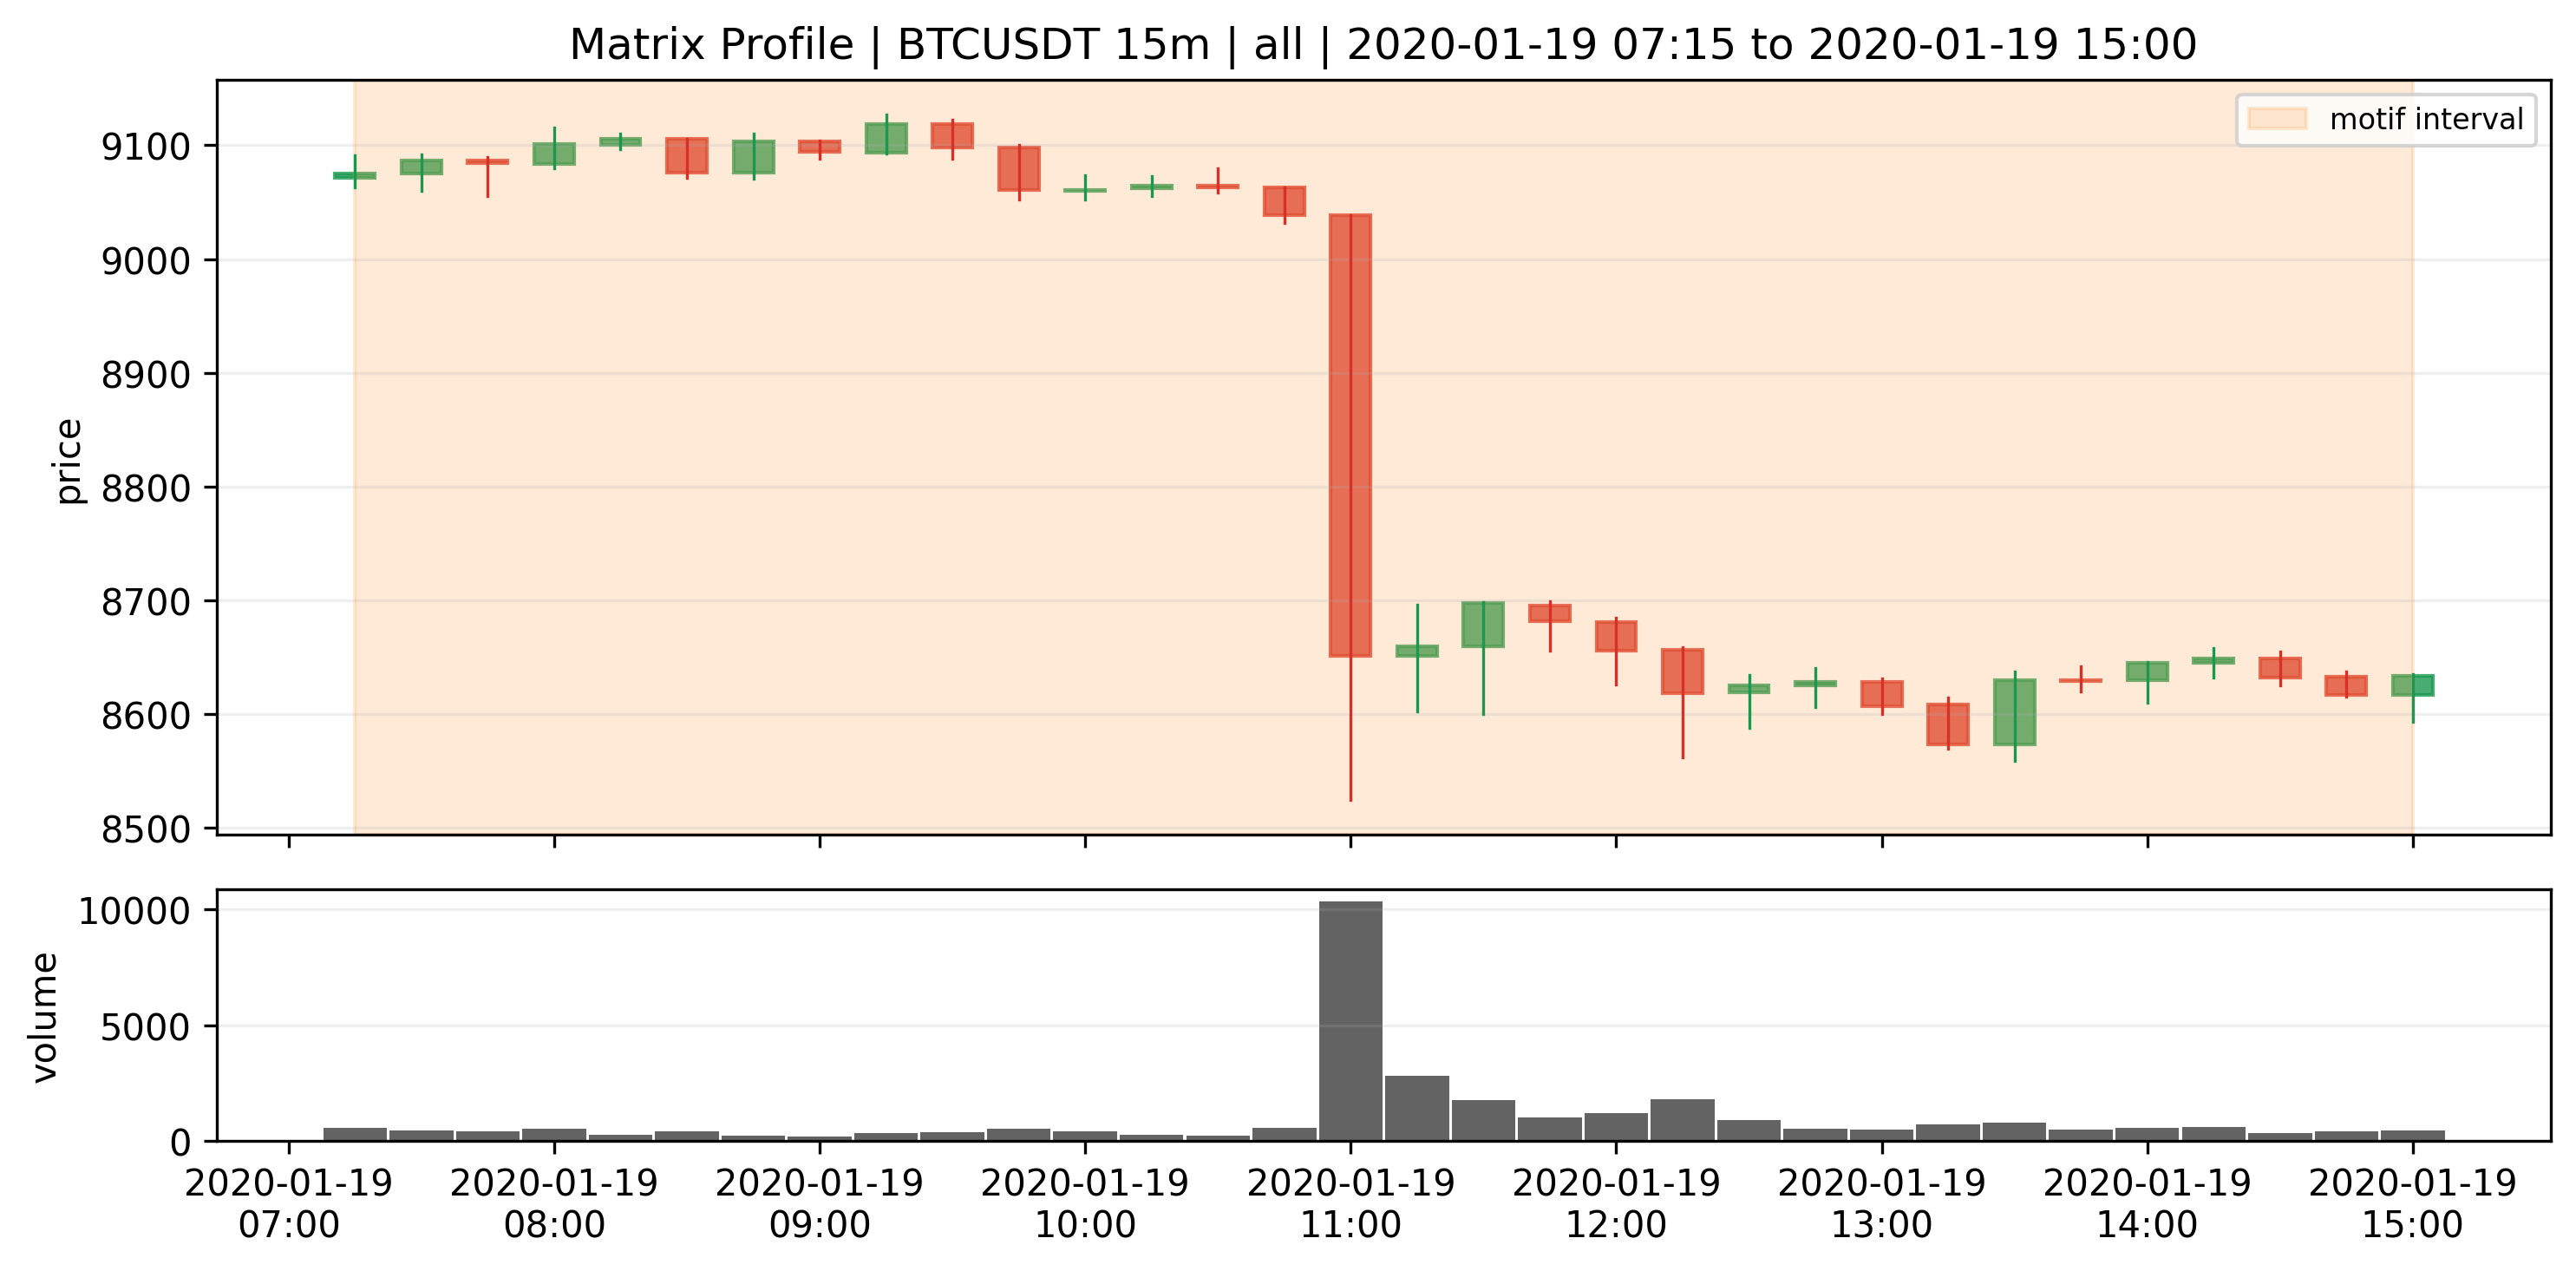
\includegraphics[width=0.9\linewidth]{reports/final_visual_evidence/figures/motif_12_matrix_profile_btcusdt_15m_all_1_0_pair21_2_zoom.png}
\caption{motif 12 matrix profile btcusdt 15m all 1 0 pair21 2 zoom. The shaded interval marks the discovered motif occurrence in original price context.}
\end{figure}

\begin{figure}[ht]
\centering
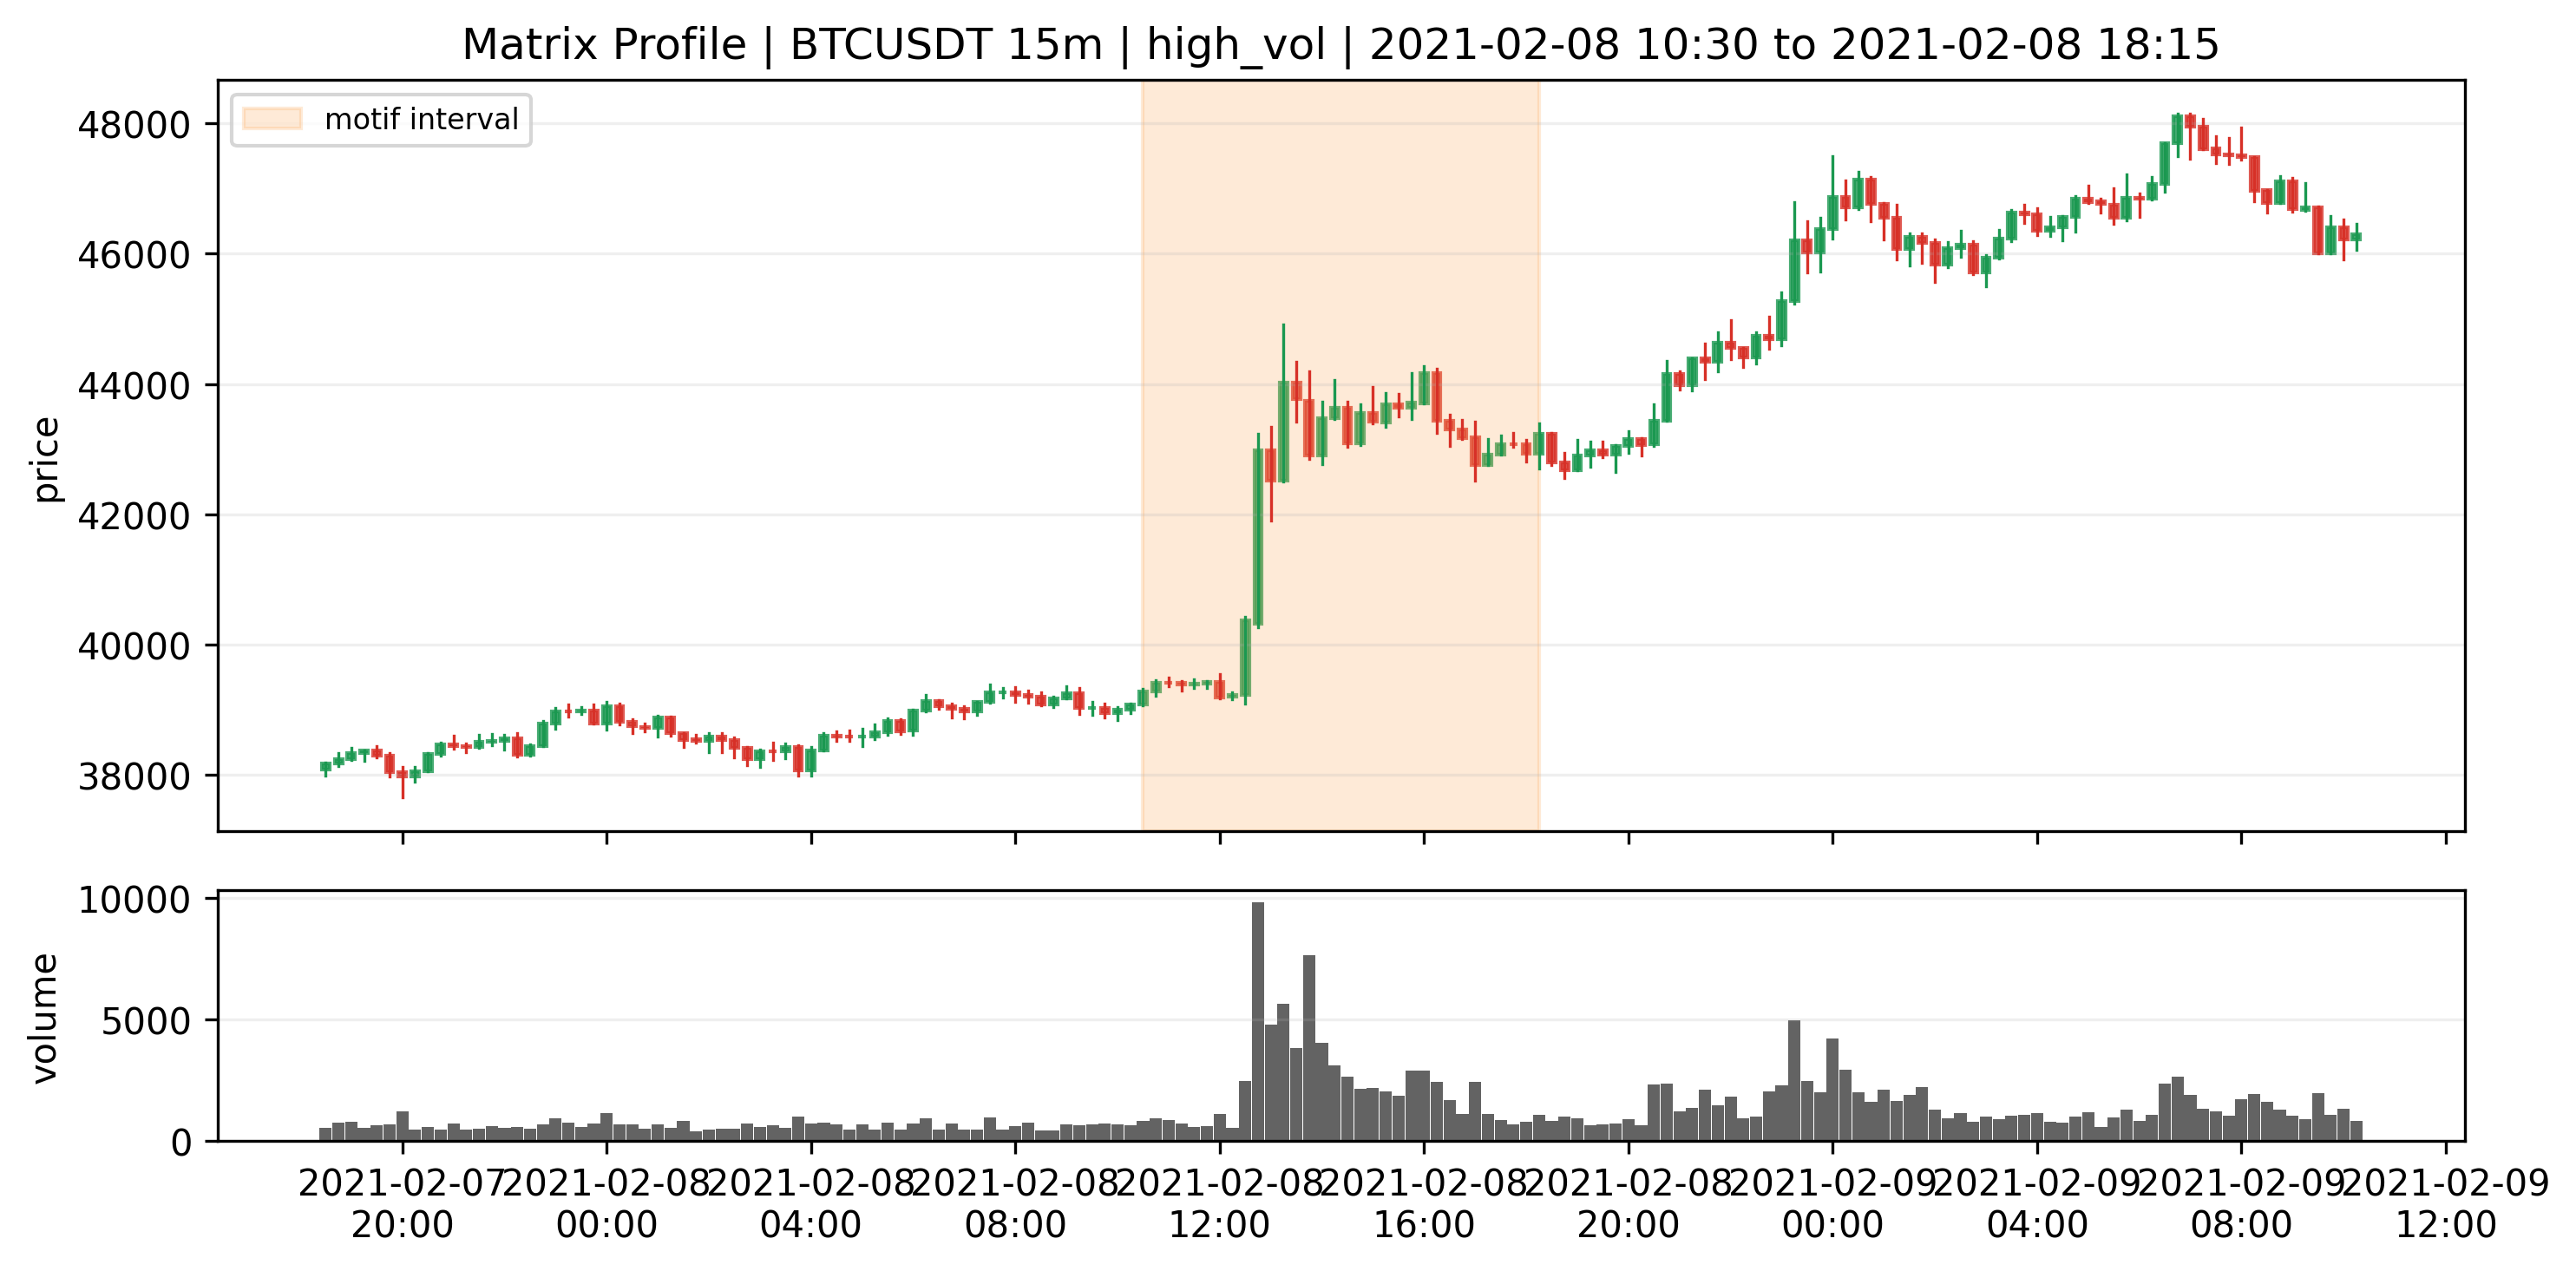
\includegraphics[width=0.9\linewidth]{reports/final_visual_evidence/figures/motif_13_matrix_profile_btcusdt_15m_high_vol_1_0_pair75_1_context.png}
\caption{motif 13 matrix profile btcusdt 15m high vol 1 0 pair75 1 context. The shaded interval marks the discovered motif occurrence in original price context.}
\end{figure}

\begin{figure}[ht]
\centering
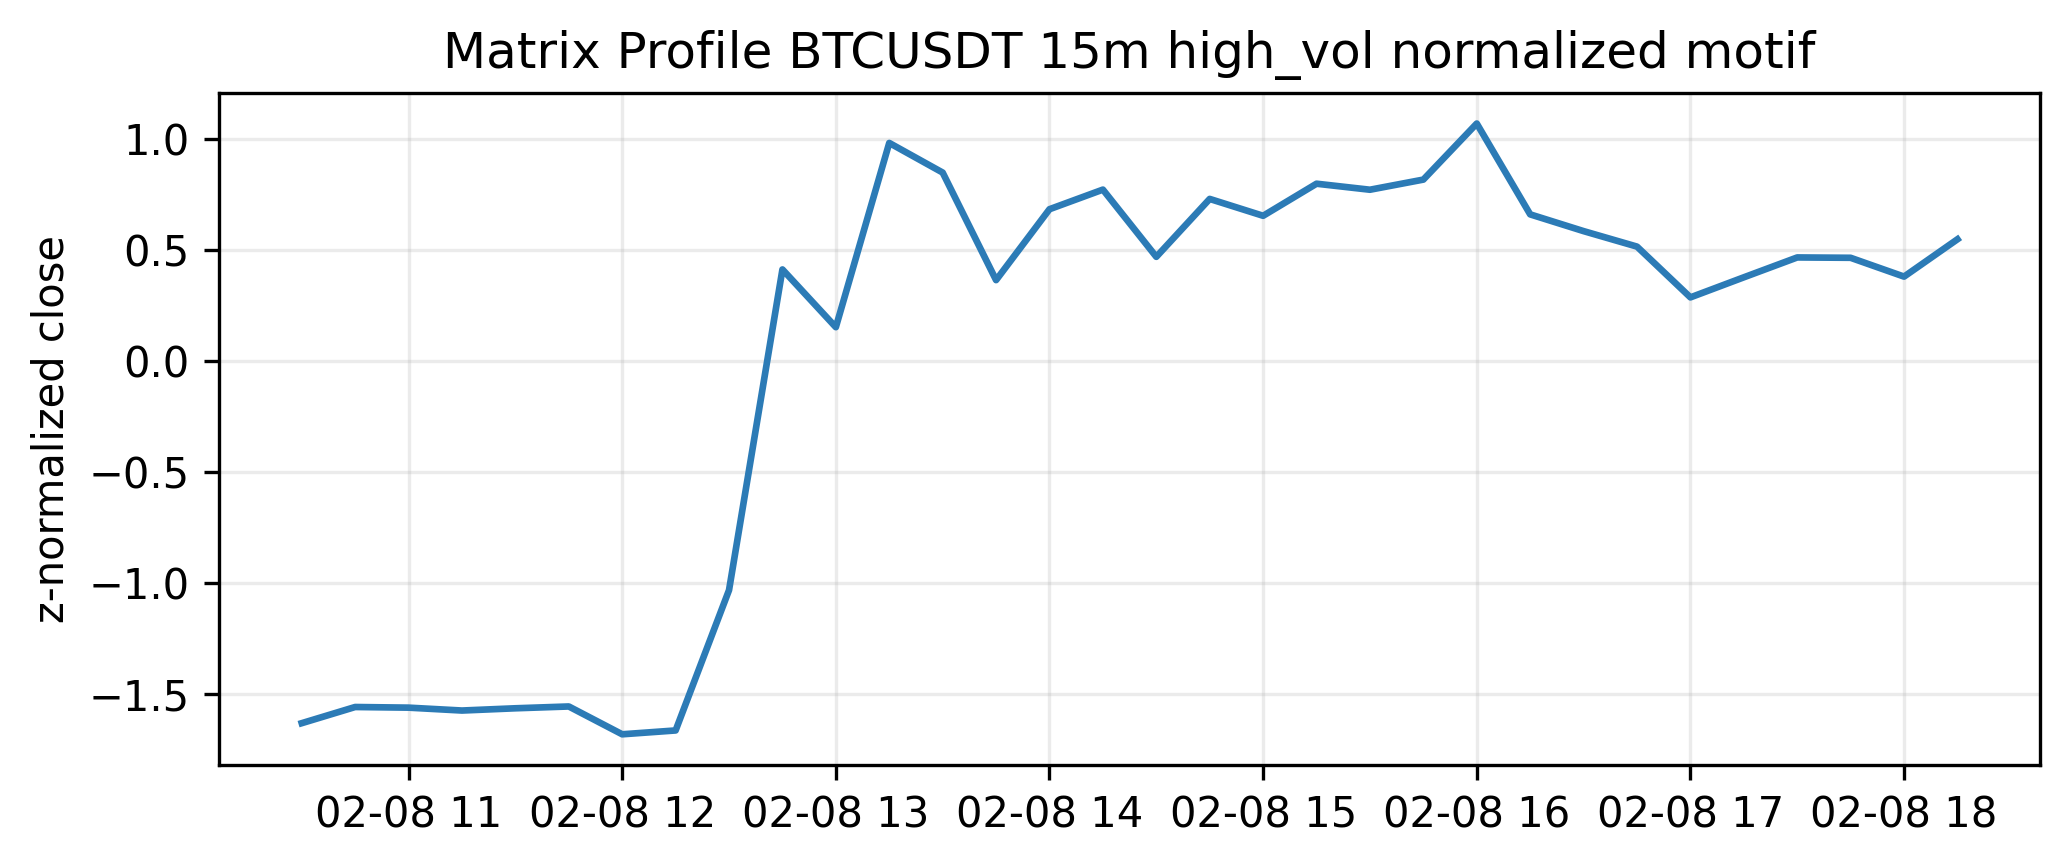
\includegraphics[width=0.9\linewidth]{reports/final_visual_evidence/figures/motif_13_matrix_profile_btcusdt_15m_high_vol_1_0_pair75_1_normal_pattern.png}
\caption{motif 13 matrix profile btcusdt 15m high vol 1 0 pair75 1 normal pattern. The shaded interval marks the discovered motif occurrence in original price context.}
\end{figure}

\begin{figure}[ht]
\centering
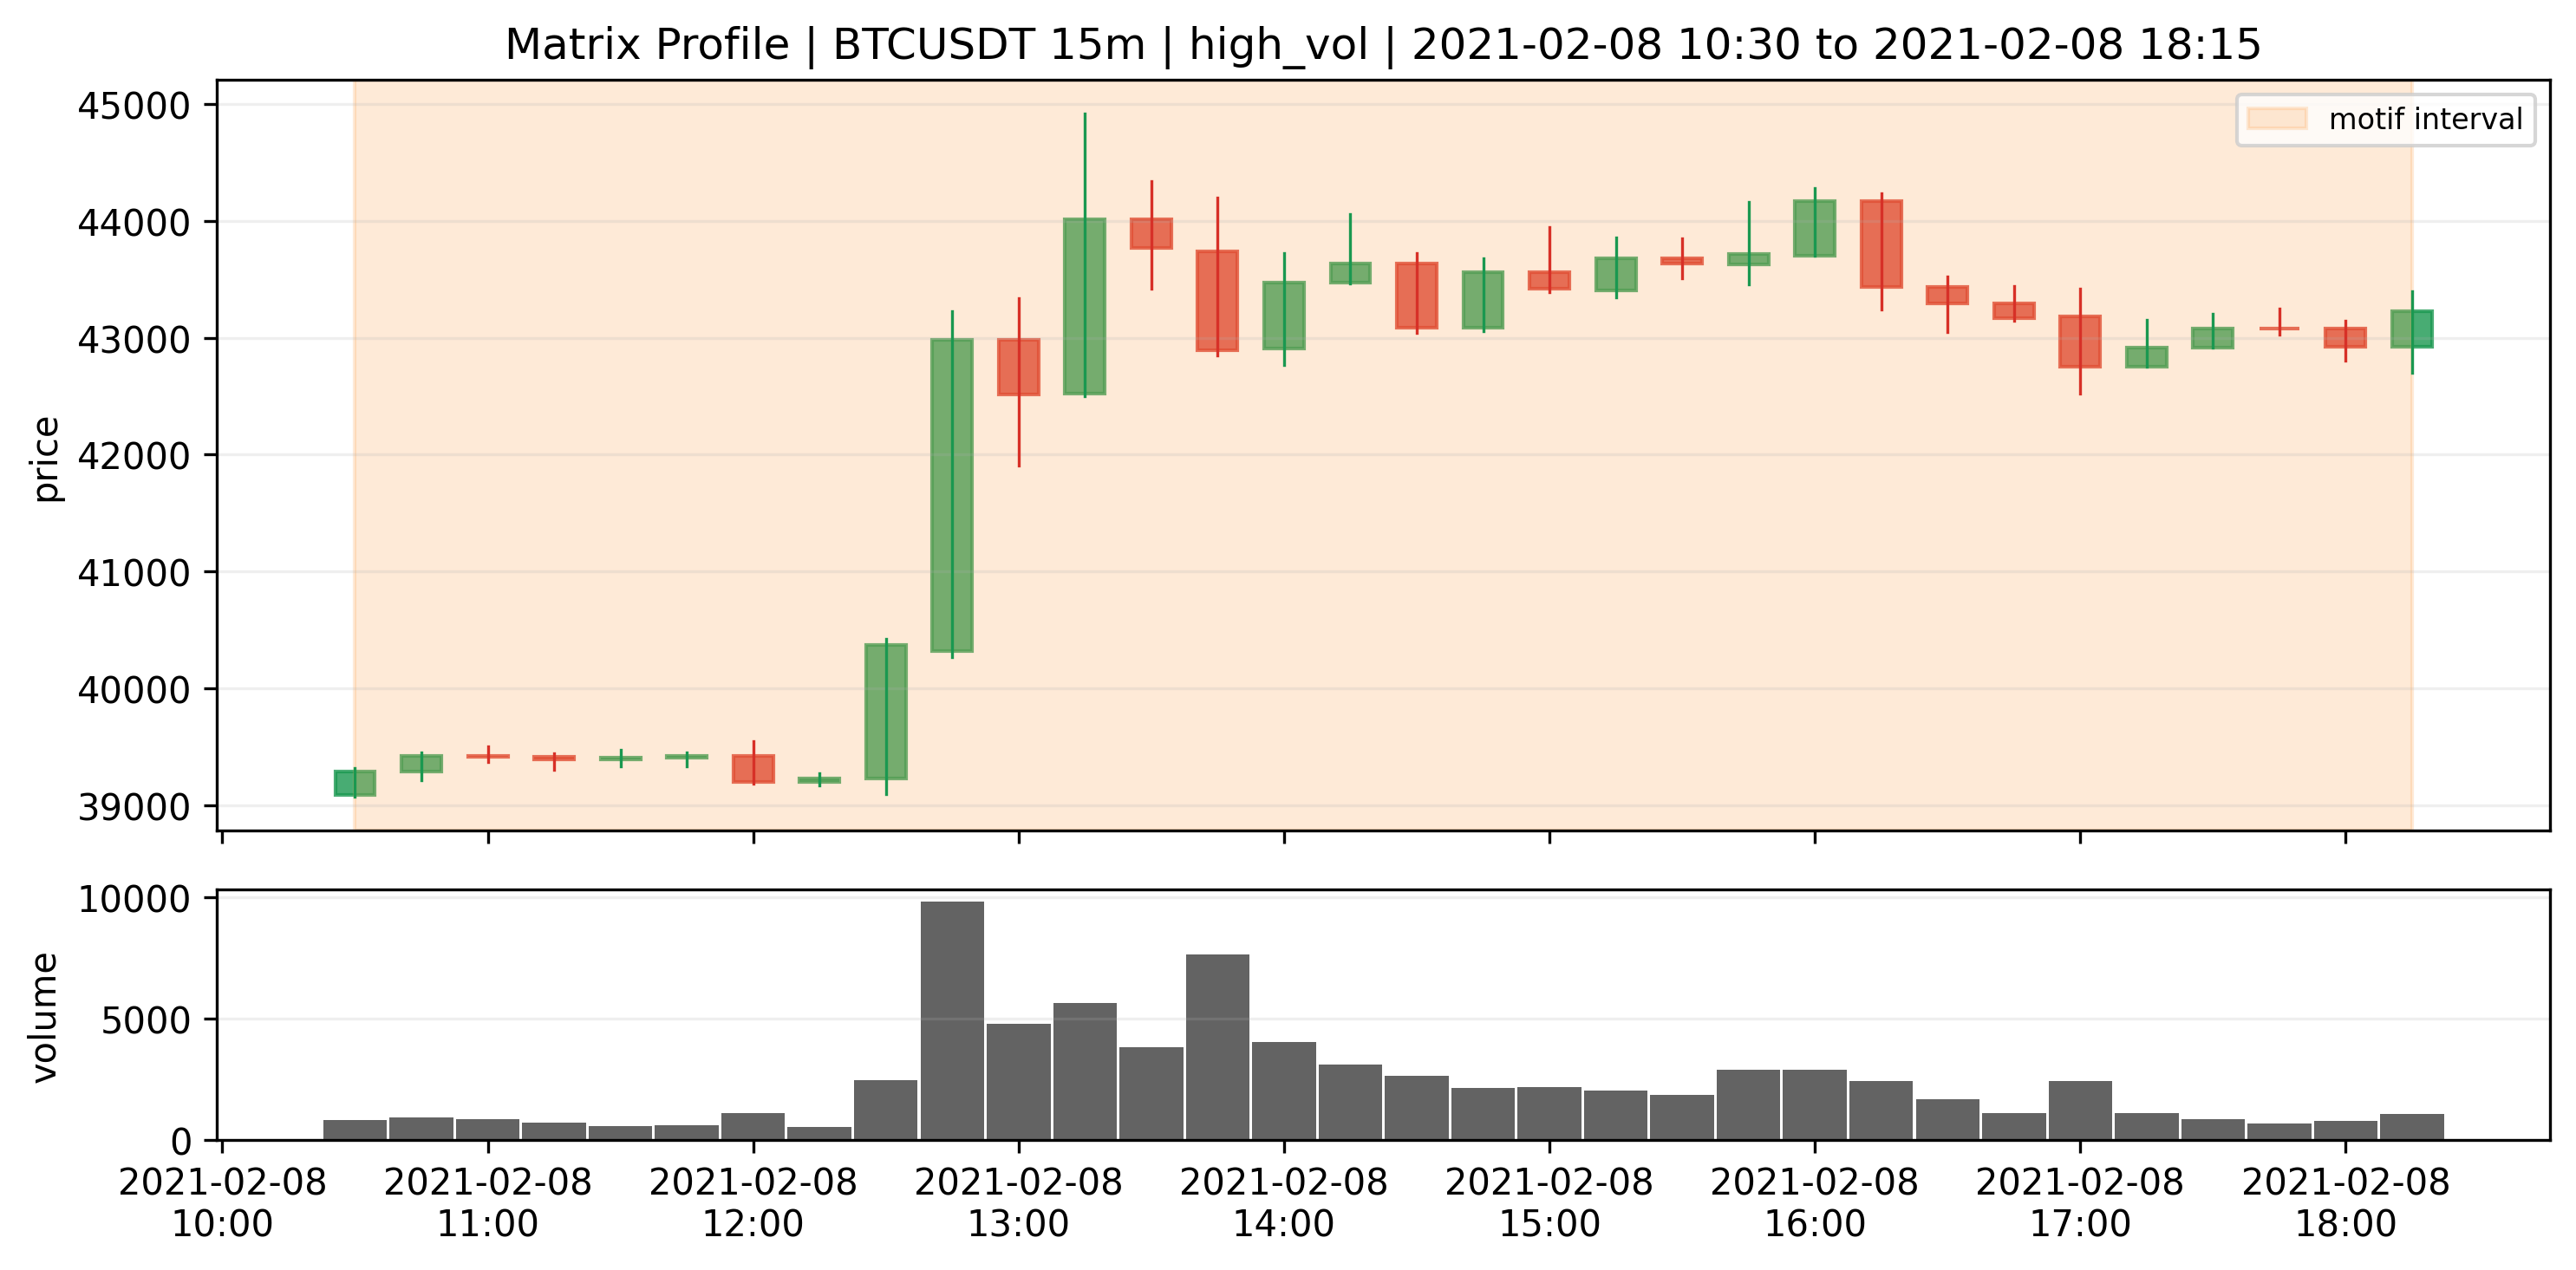
\includegraphics[width=0.9\linewidth]{reports/final_visual_evidence/figures/motif_13_matrix_profile_btcusdt_15m_high_vol_1_0_pair75_1_zoom.png}
\caption{motif 13 matrix profile btcusdt 15m high vol 1 0 pair75 1 zoom. The shaded interval marks the discovered motif occurrence in original price context.}
\end{figure}

\begin{figure}[ht]
\centering
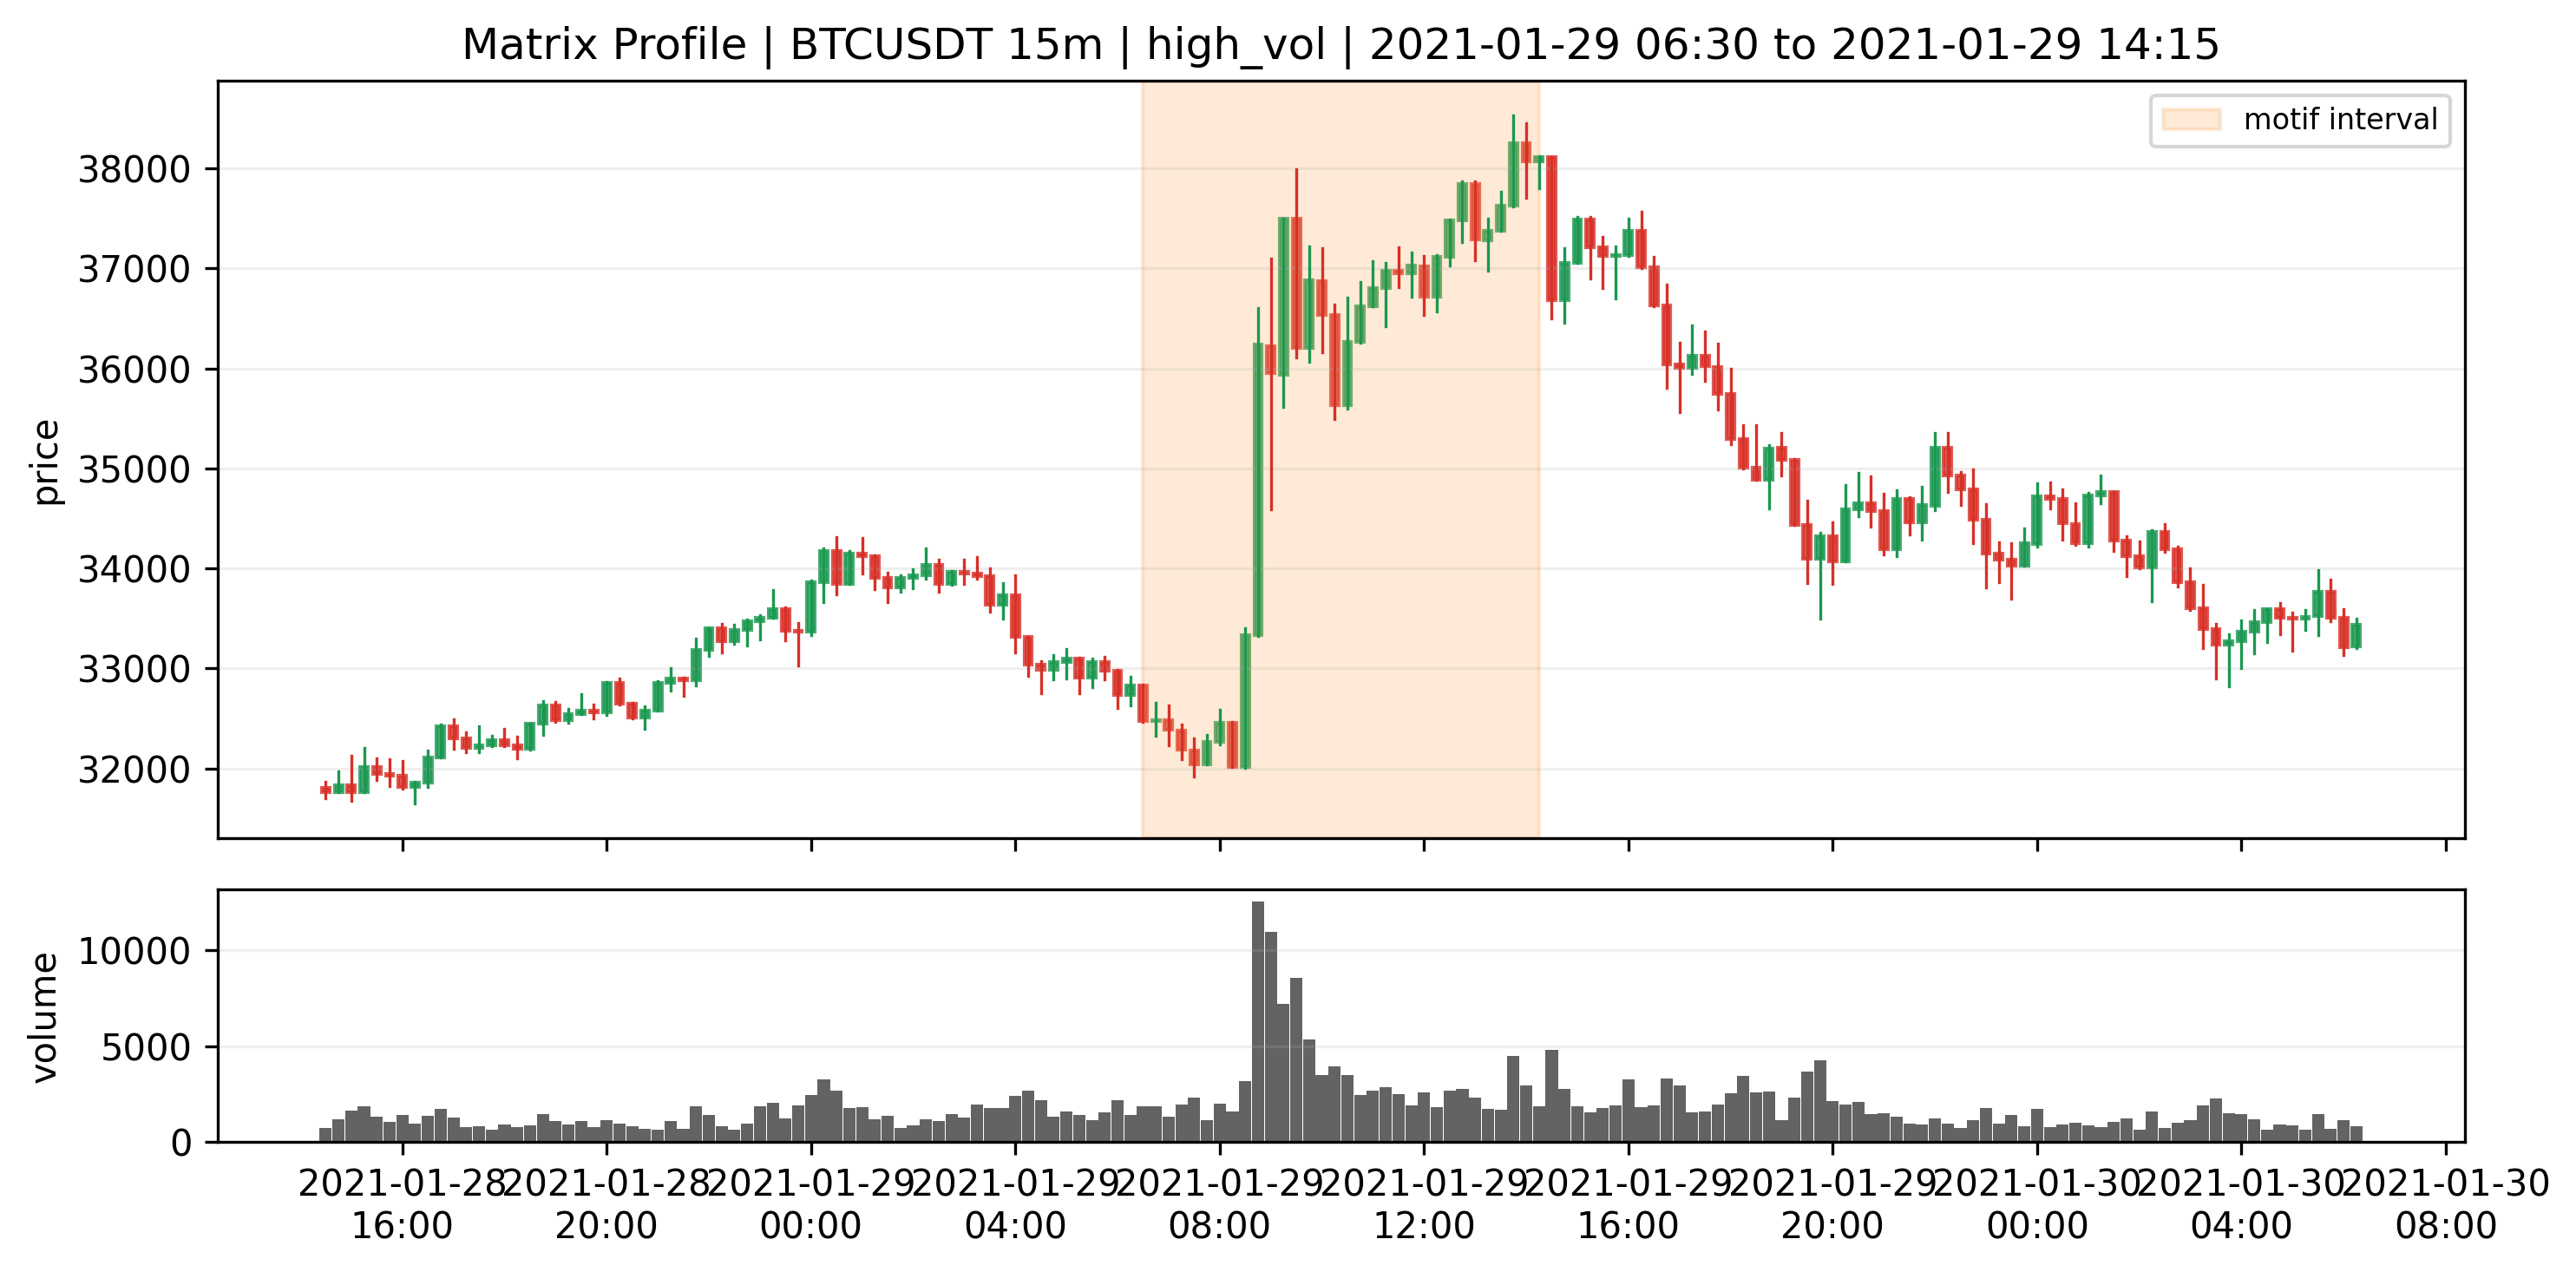
\includegraphics[width=0.9\linewidth]{reports/final_visual_evidence/figures/motif_14_matrix_profile_btcusdt_15m_high_vol_1_0_pair75_2_context.png}
\caption{motif 14 matrix profile btcusdt 15m high vol 1 0 pair75 2 context. The shaded interval marks the discovered motif occurrence in original price context.}
\end{figure}

\begin{figure}[ht]
\centering
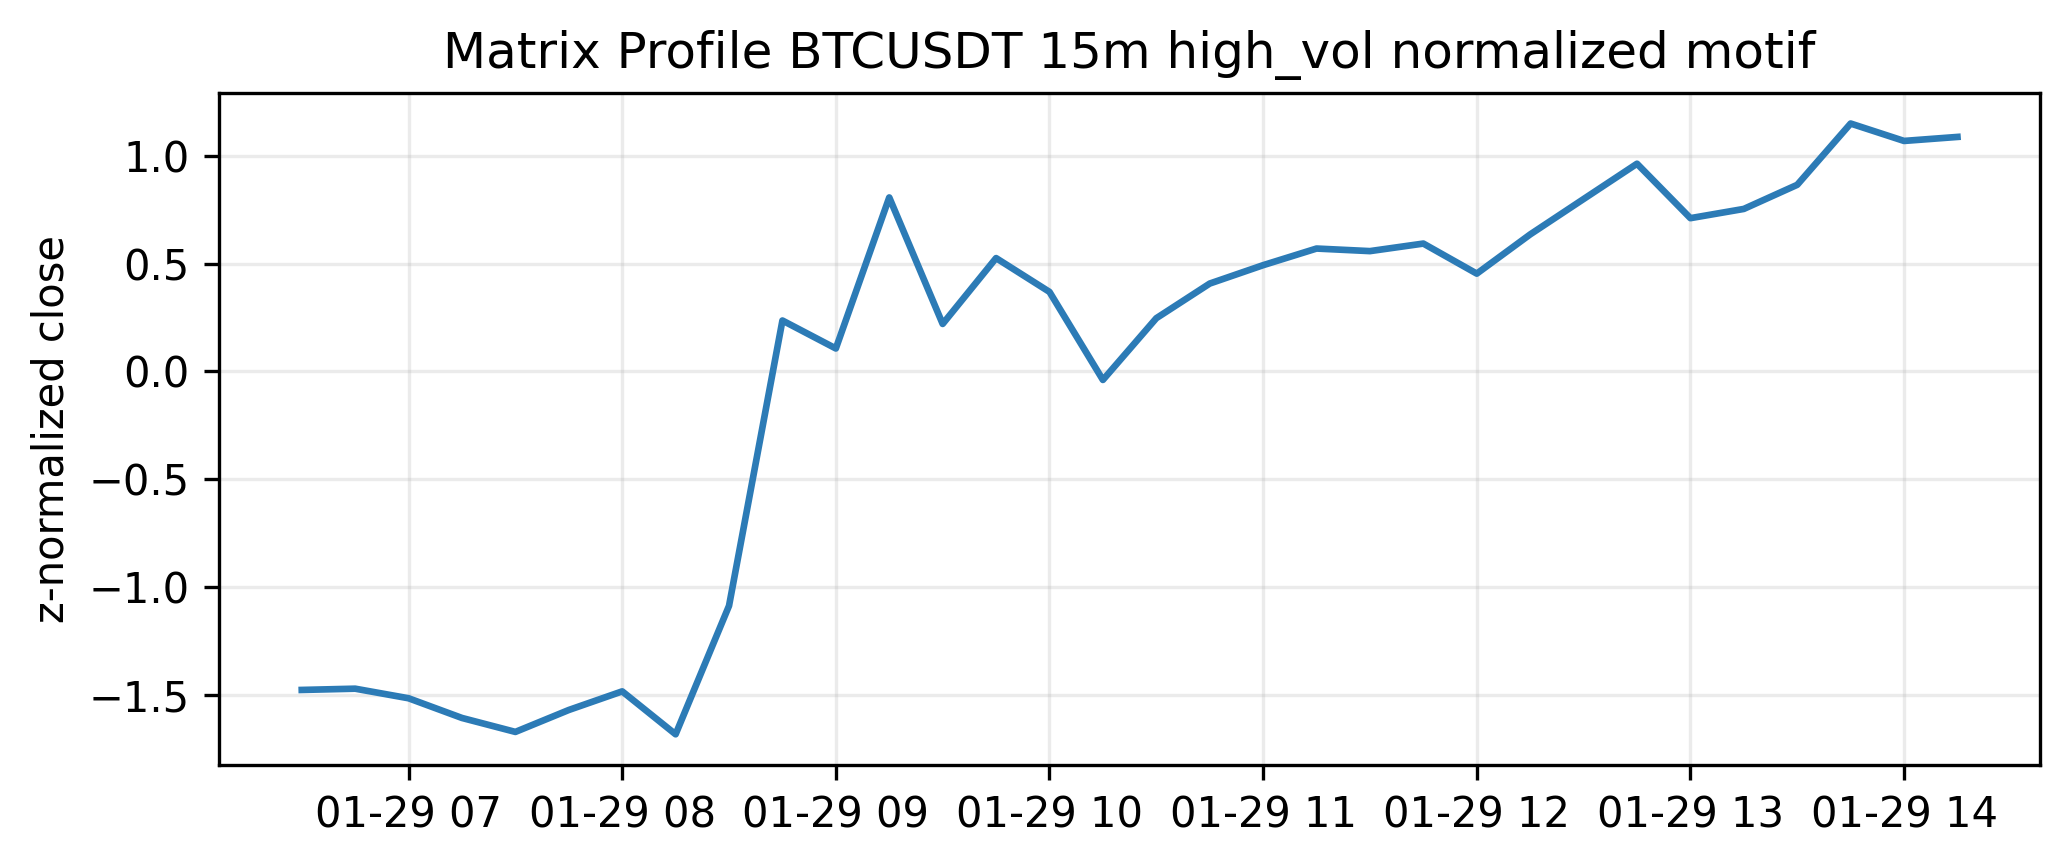
\includegraphics[width=0.9\linewidth]{reports/final_visual_evidence/figures/motif_14_matrix_profile_btcusdt_15m_high_vol_1_0_pair75_2_normal_pattern.png}
\caption{motif 14 matrix profile btcusdt 15m high vol 1 0 pair75 2 normal pattern. The shaded interval marks the discovered motif occurrence in original price context.}
\end{figure}

\begin{figure}[ht]
\centering
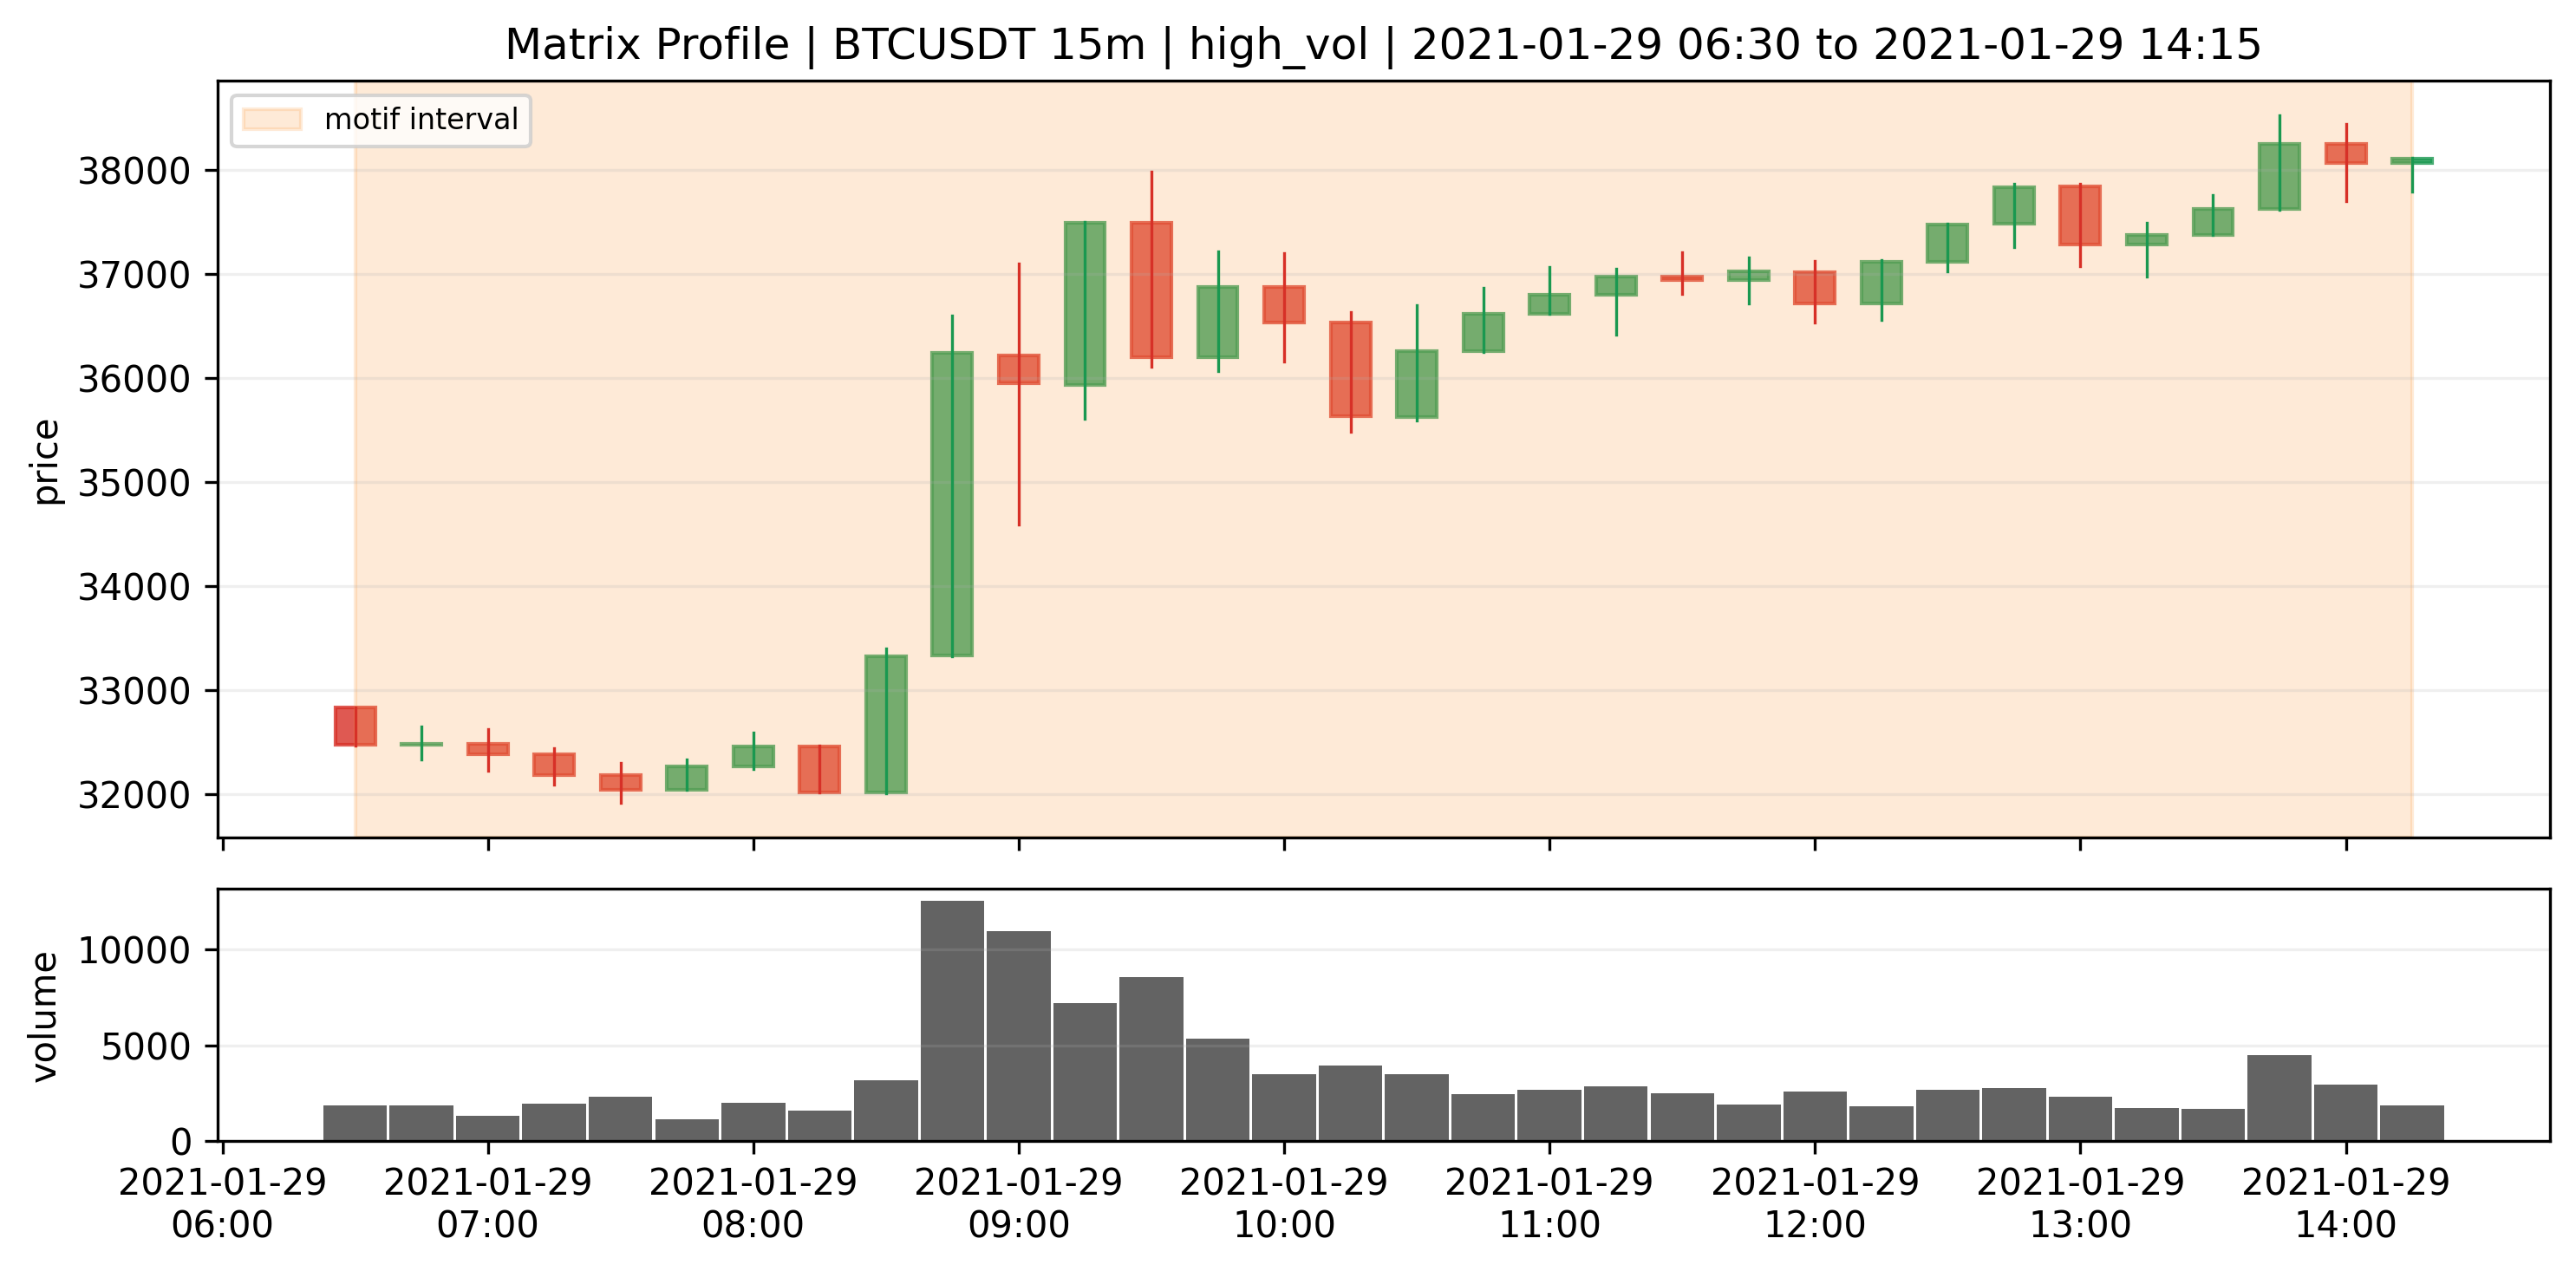
\includegraphics[width=0.9\linewidth]{reports/final_visual_evidence/figures/motif_14_matrix_profile_btcusdt_15m_high_vol_1_0_pair75_2_zoom.png}
\caption{motif 14 matrix profile btcusdt 15m high vol 1 0 pair75 2 zoom. The shaded interval marks the discovered motif occurrence in original price context.}
\end{figure}

\begin{figure}[ht]
\centering
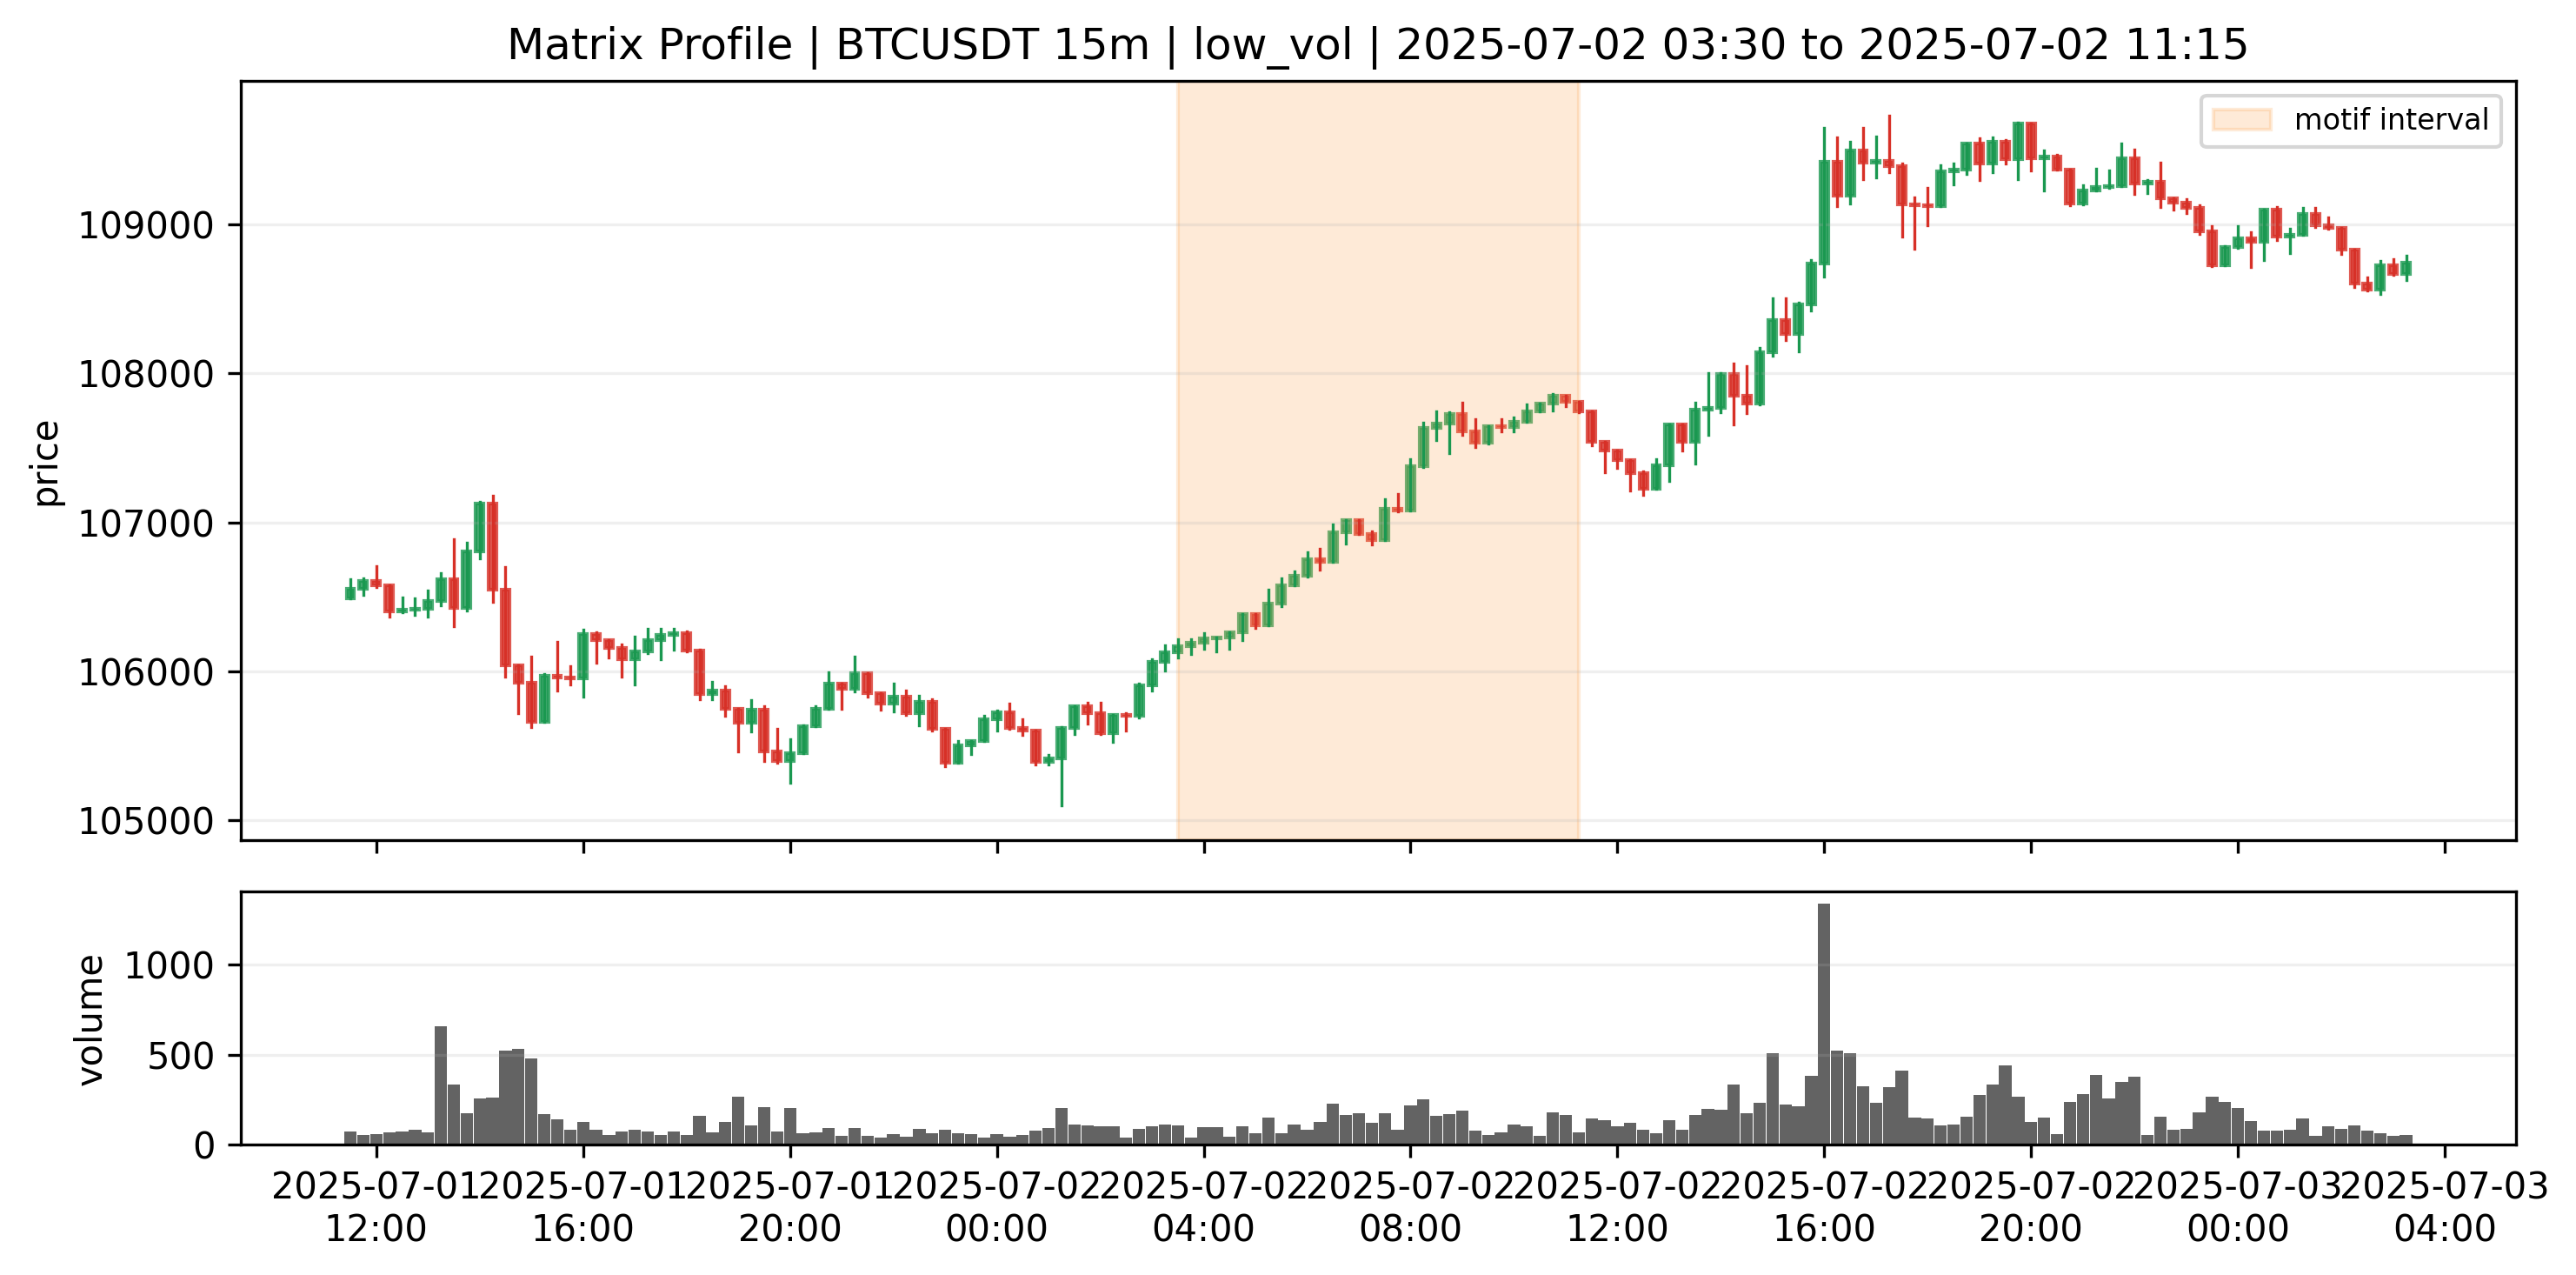
\includegraphics[width=0.9\linewidth]{reports/final_visual_evidence/figures/motif_15_matrix_profile_btcusdt_15m_low_vol_nan_pair7_1_context.png}
\caption{motif 15 matrix profile btcusdt 15m low vol nan pair7 1 context. The shaded interval marks the discovered motif occurrence in original price context.}
\end{figure}

\begin{figure}[ht]
\centering
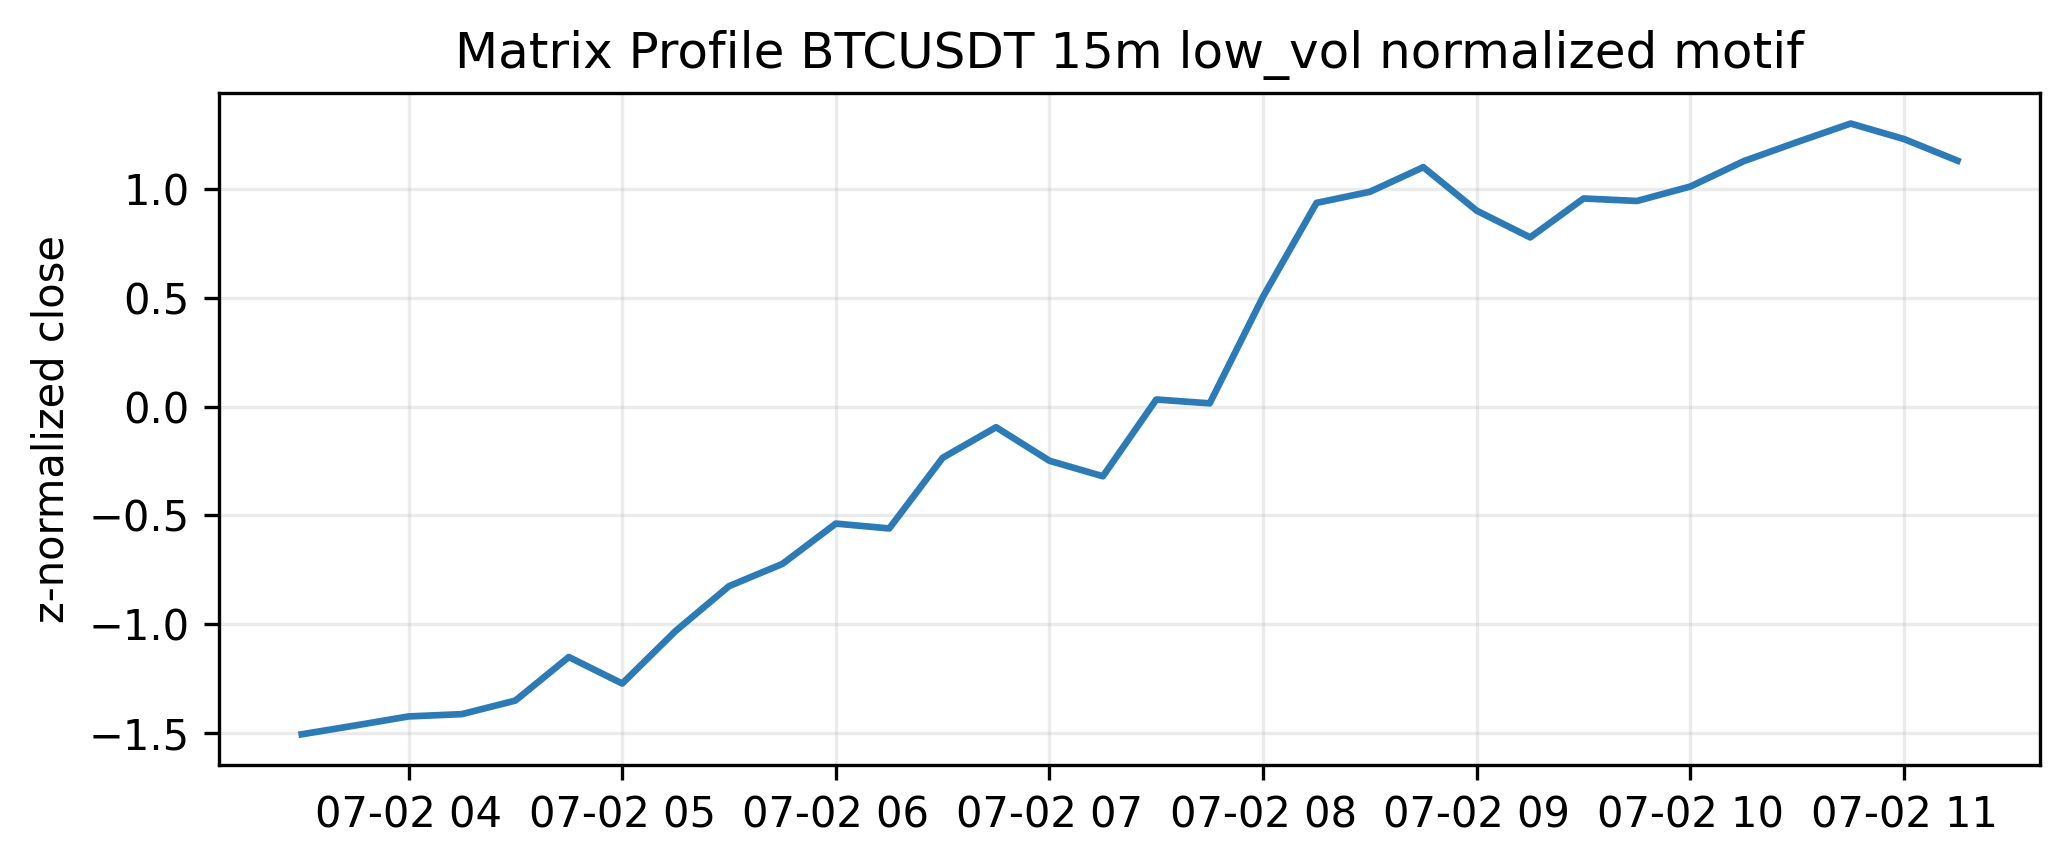
\includegraphics[width=0.9\linewidth]{reports/final_visual_evidence/figures/motif_15_matrix_profile_btcusdt_15m_low_vol_nan_pair7_1_normal_pattern.png}
\caption{motif 15 matrix profile btcusdt 15m low vol nan pair7 1 normal pattern. The shaded interval marks the discovered motif occurrence in original price context.}
\end{figure}

\begin{figure}[ht]
\centering
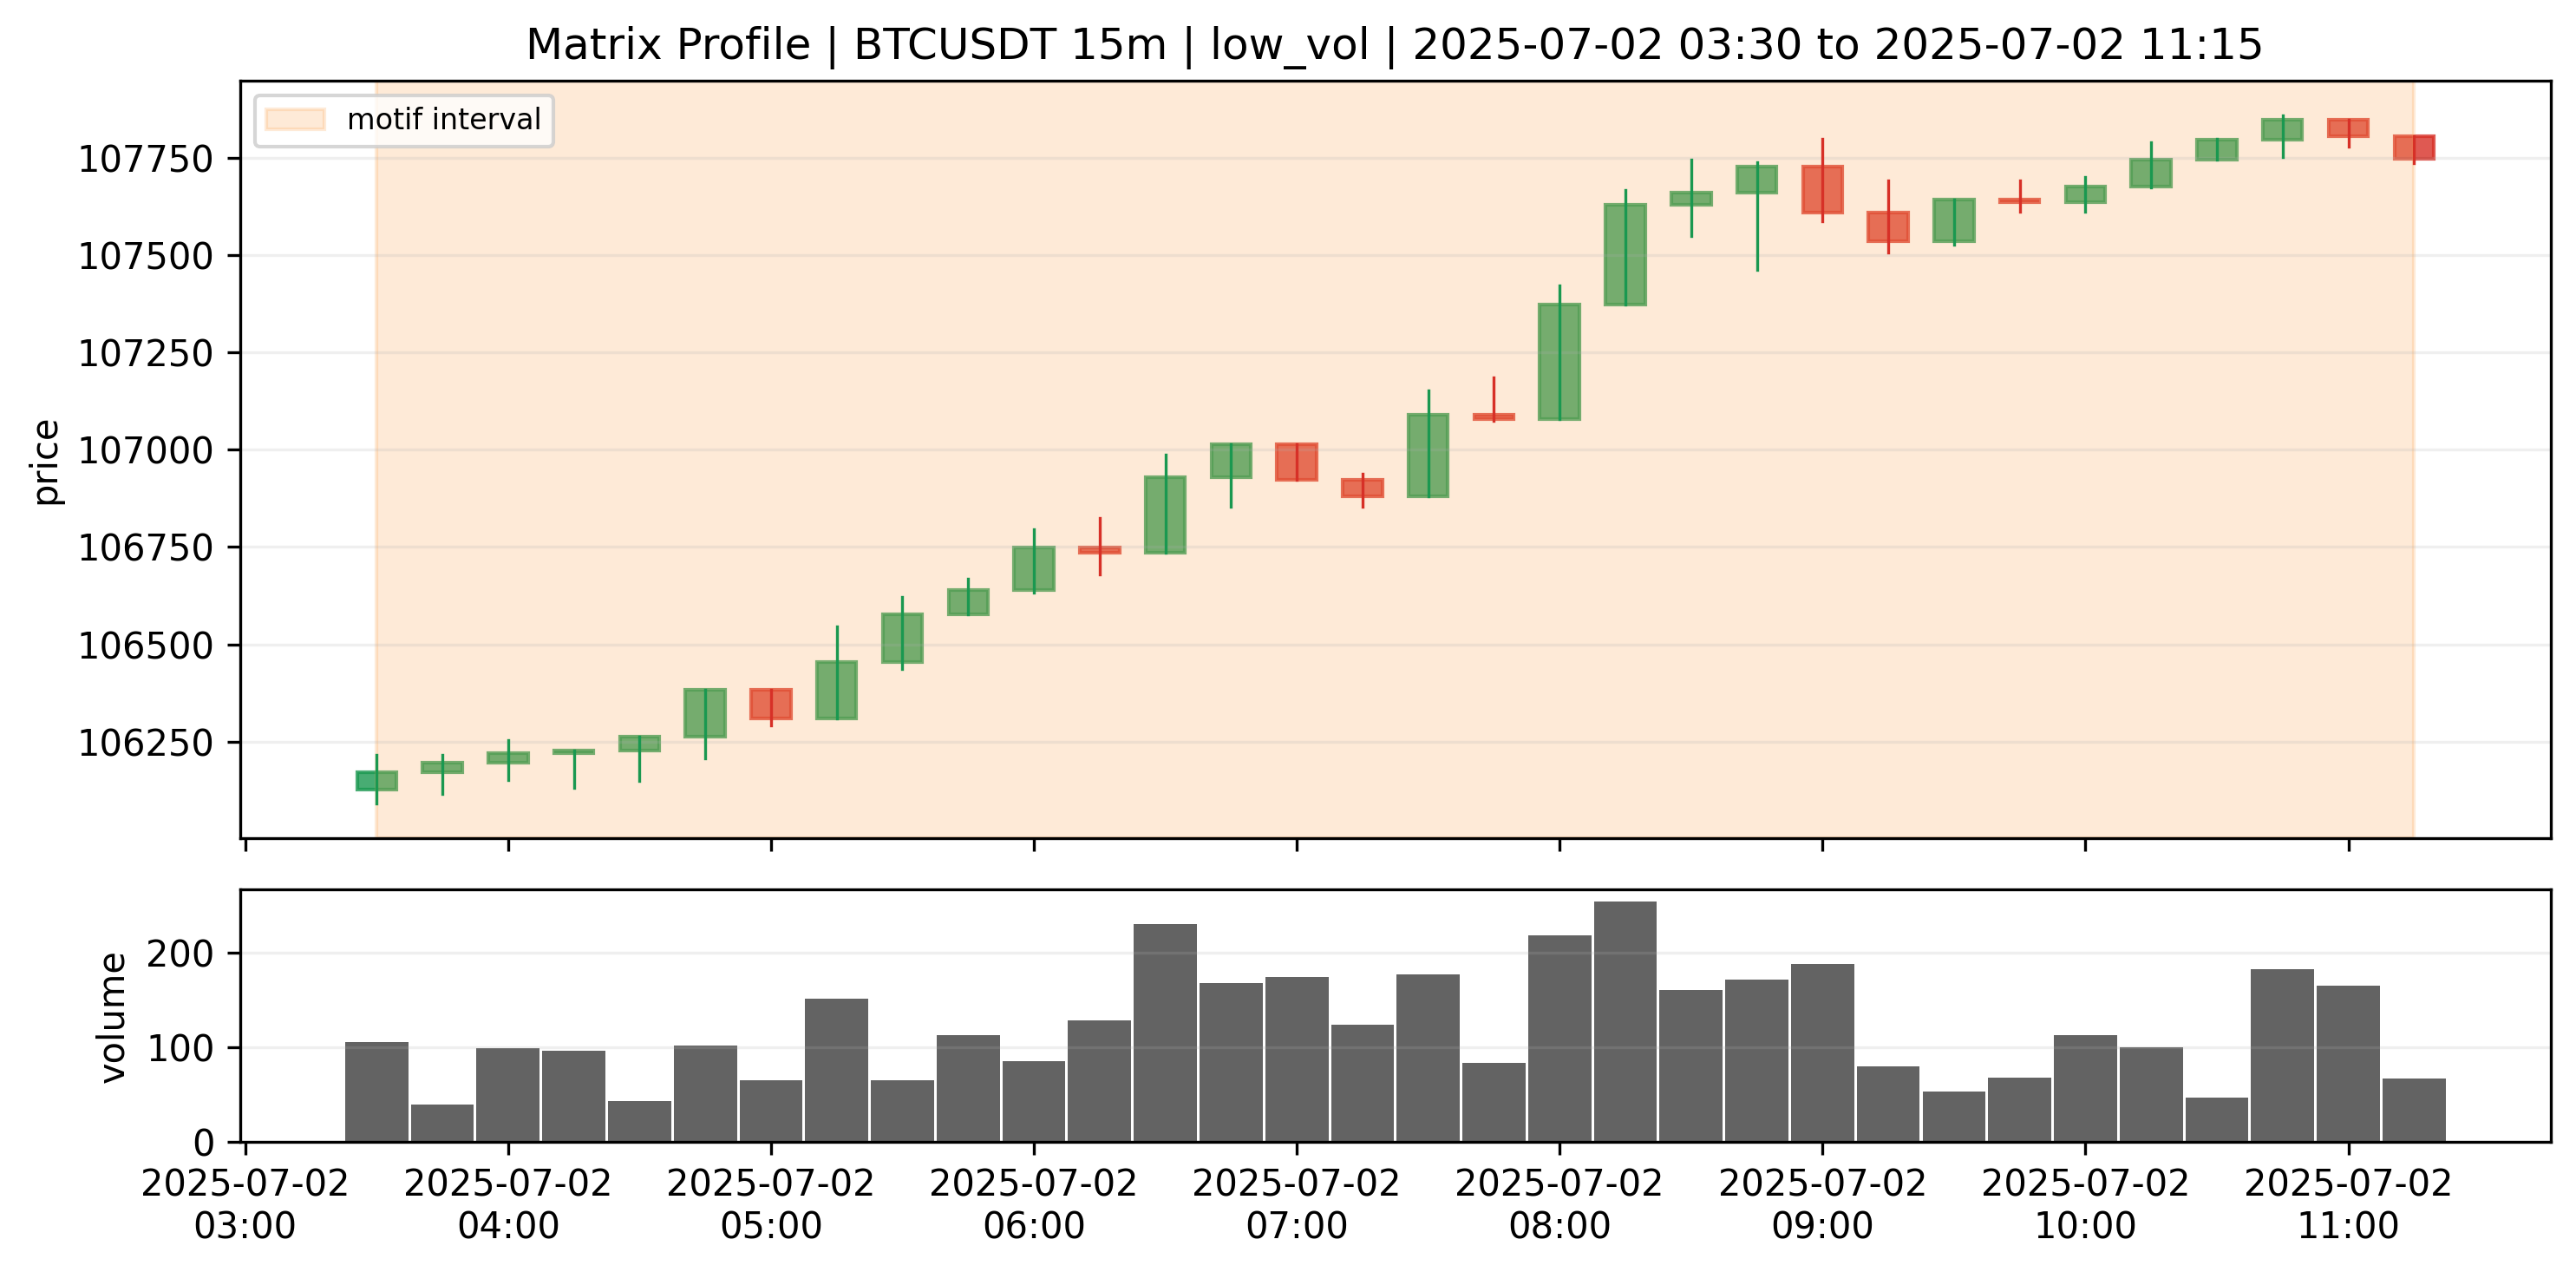
\includegraphics[width=0.9\linewidth]{reports/final_visual_evidence/figures/motif_15_matrix_profile_btcusdt_15m_low_vol_nan_pair7_1_zoom.png}
\caption{motif 15 matrix profile btcusdt 15m low vol nan pair7 1 zoom. The shaded interval marks the discovered motif occurrence in original price context.}
\end{figure}

\begin{figure}[ht]
\centering
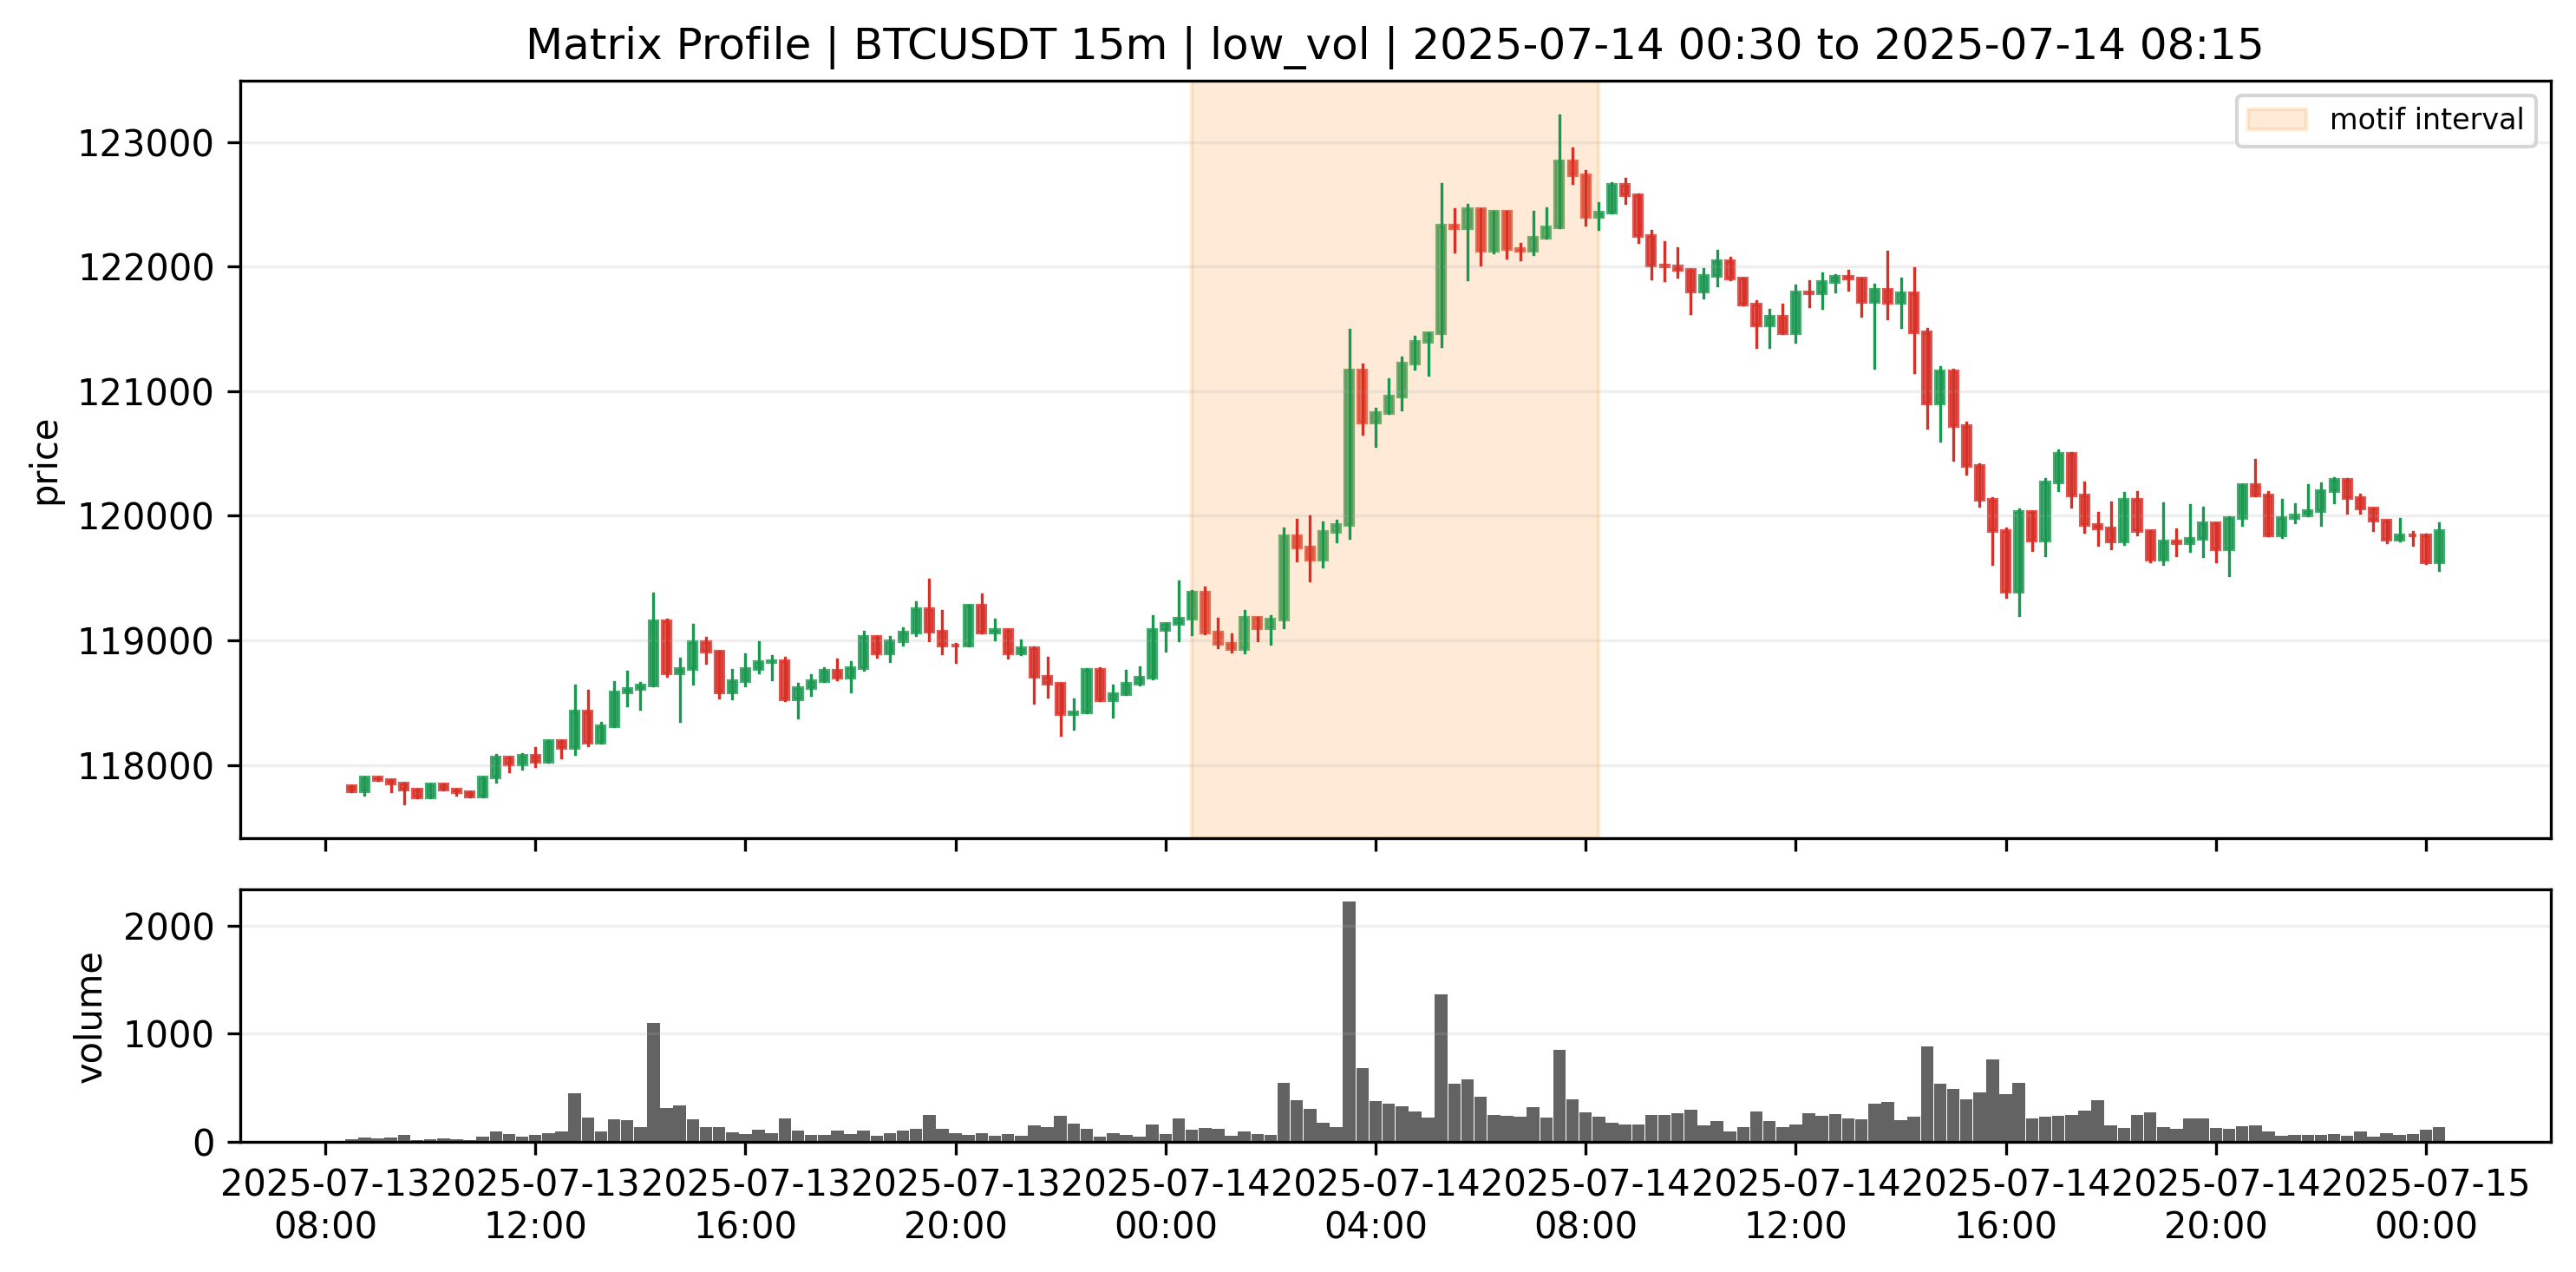
\includegraphics[width=0.9\linewidth]{reports/final_visual_evidence/figures/motif_16_matrix_profile_btcusdt_15m_low_vol_nan_pair7_2_context.png}
\caption{motif 16 matrix profile btcusdt 15m low vol nan pair7 2 context. The shaded interval marks the discovered motif occurrence in original price context.}
\end{figure}

\begin{figure}[ht]
\centering
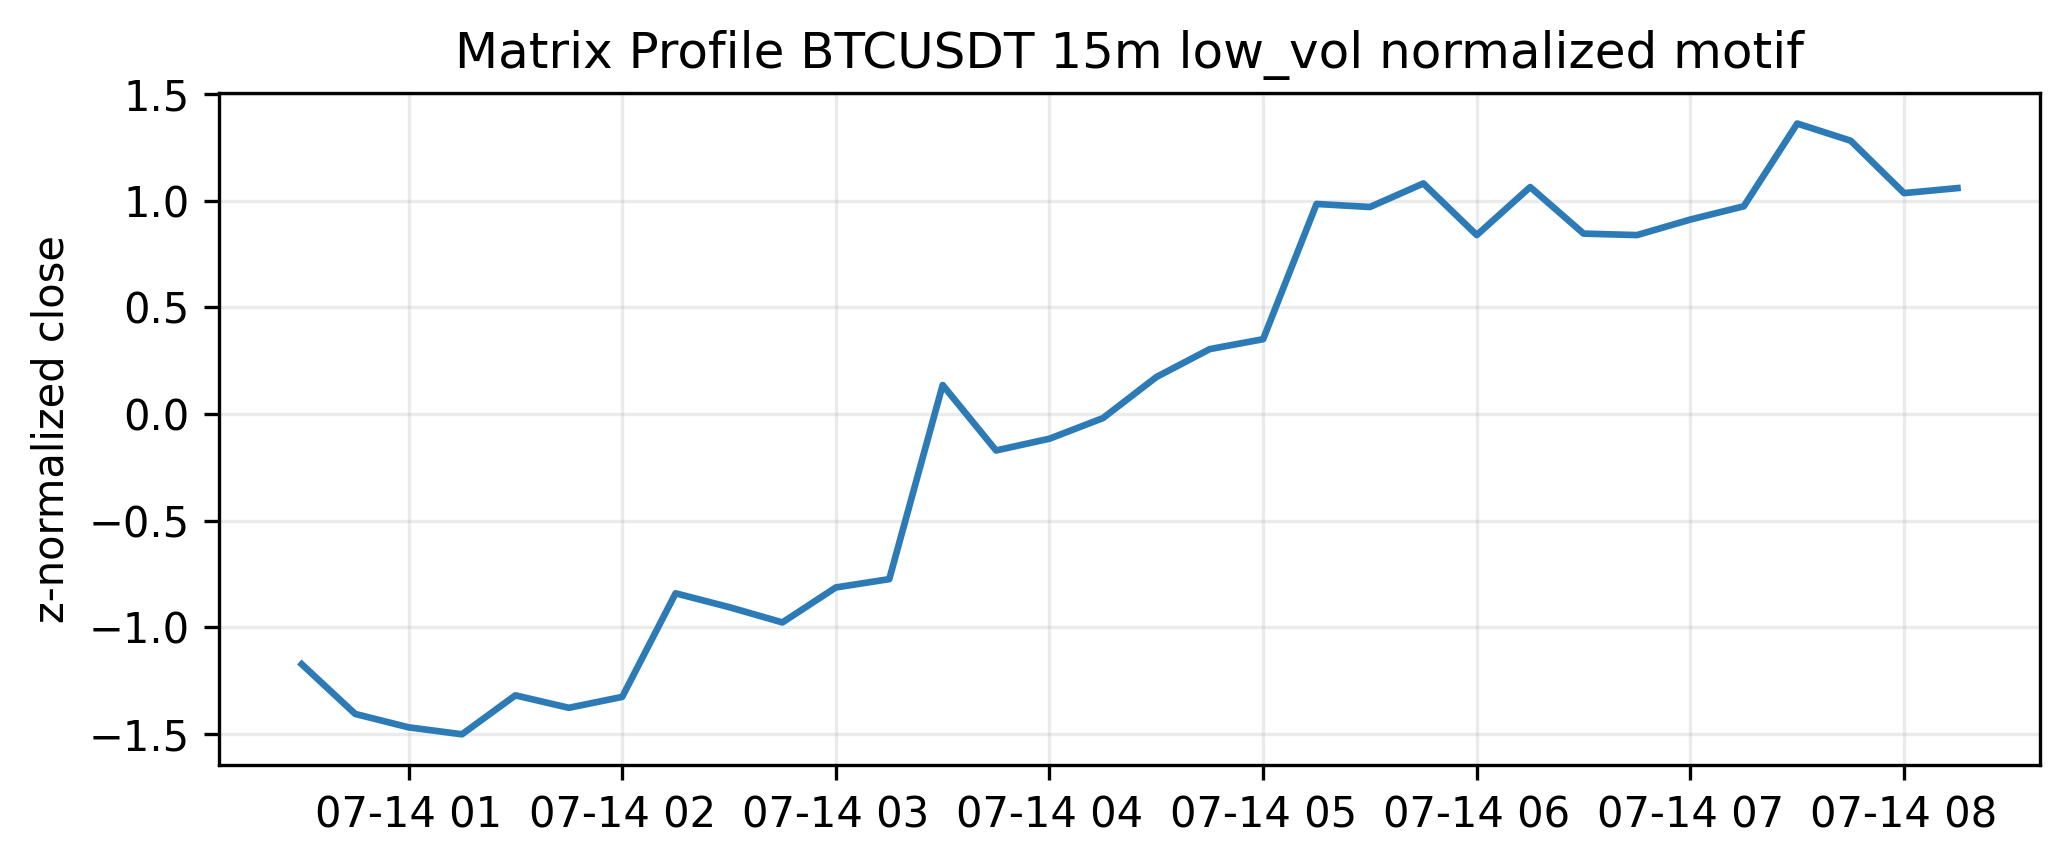
\includegraphics[width=0.9\linewidth]{reports/final_visual_evidence/figures/motif_16_matrix_profile_btcusdt_15m_low_vol_nan_pair7_2_normal_pattern.png}
\caption{motif 16 matrix profile btcusdt 15m low vol nan pair7 2 normal pattern. The shaded interval marks the discovered motif occurrence in original price context.}
\end{figure}

\begin{figure}[ht]
\centering
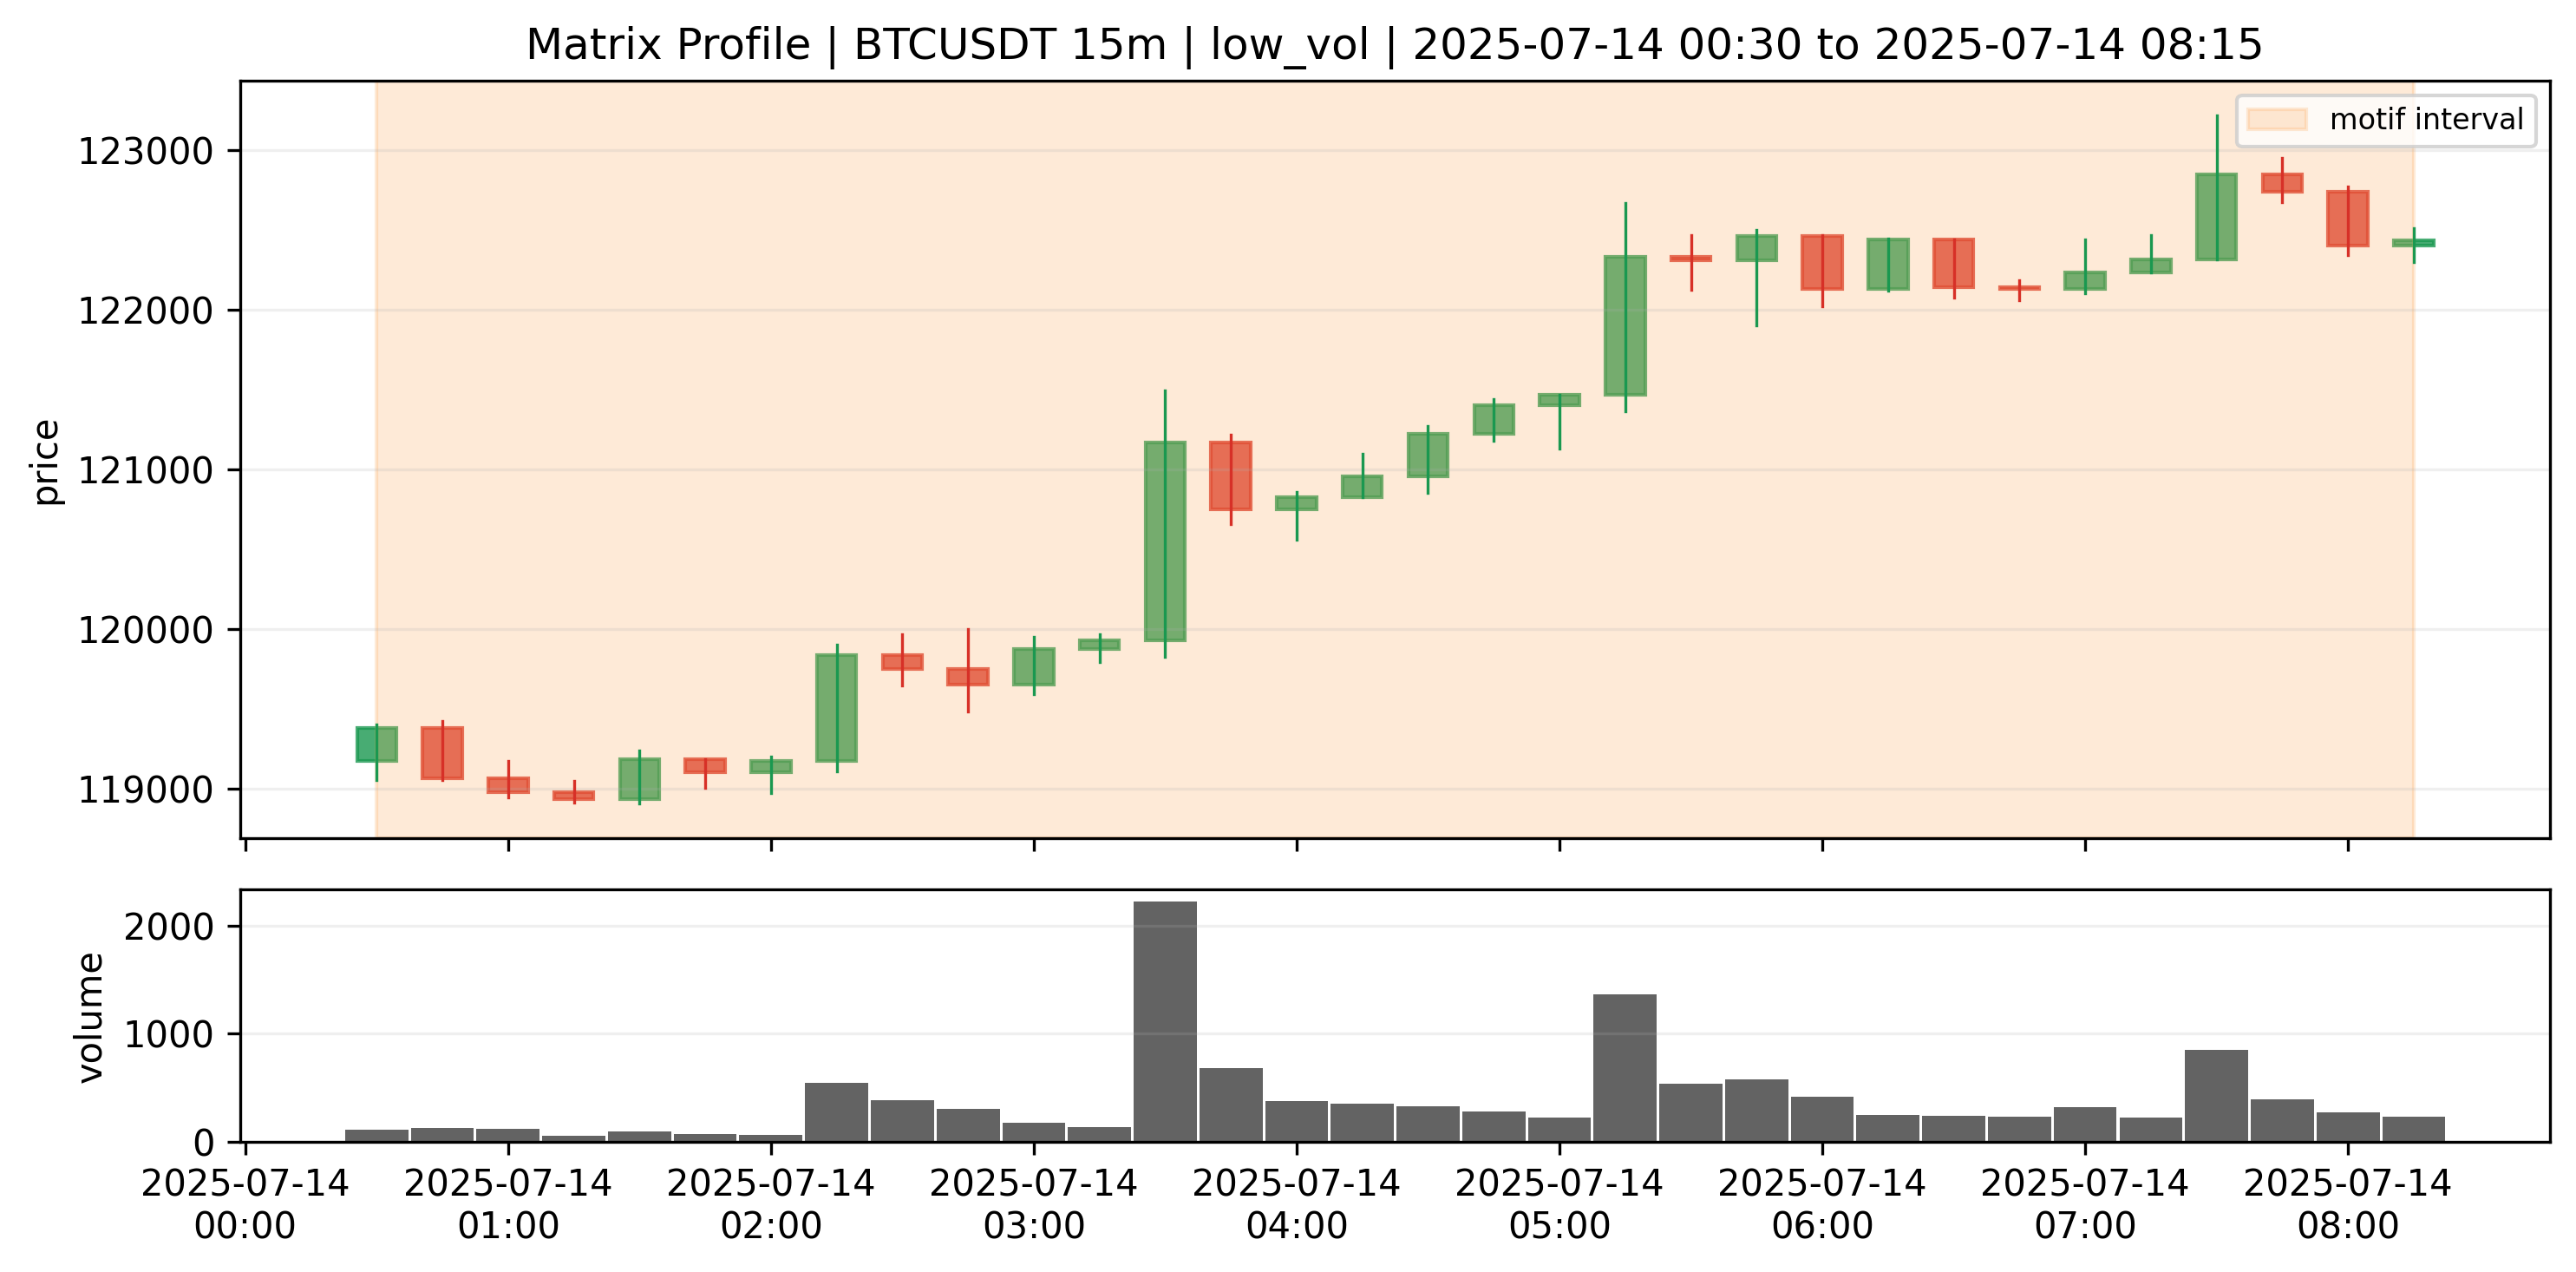
\includegraphics[width=0.9\linewidth]{reports/final_visual_evidence/figures/motif_16_matrix_profile_btcusdt_15m_low_vol_nan_pair7_2_zoom.png}
\caption{motif 16 matrix profile btcusdt 15m low vol nan pair7 2 zoom. The shaded interval marks the discovered motif occurrence in original price context.}
\end{figure}

\begin{figure}[ht]
\centering
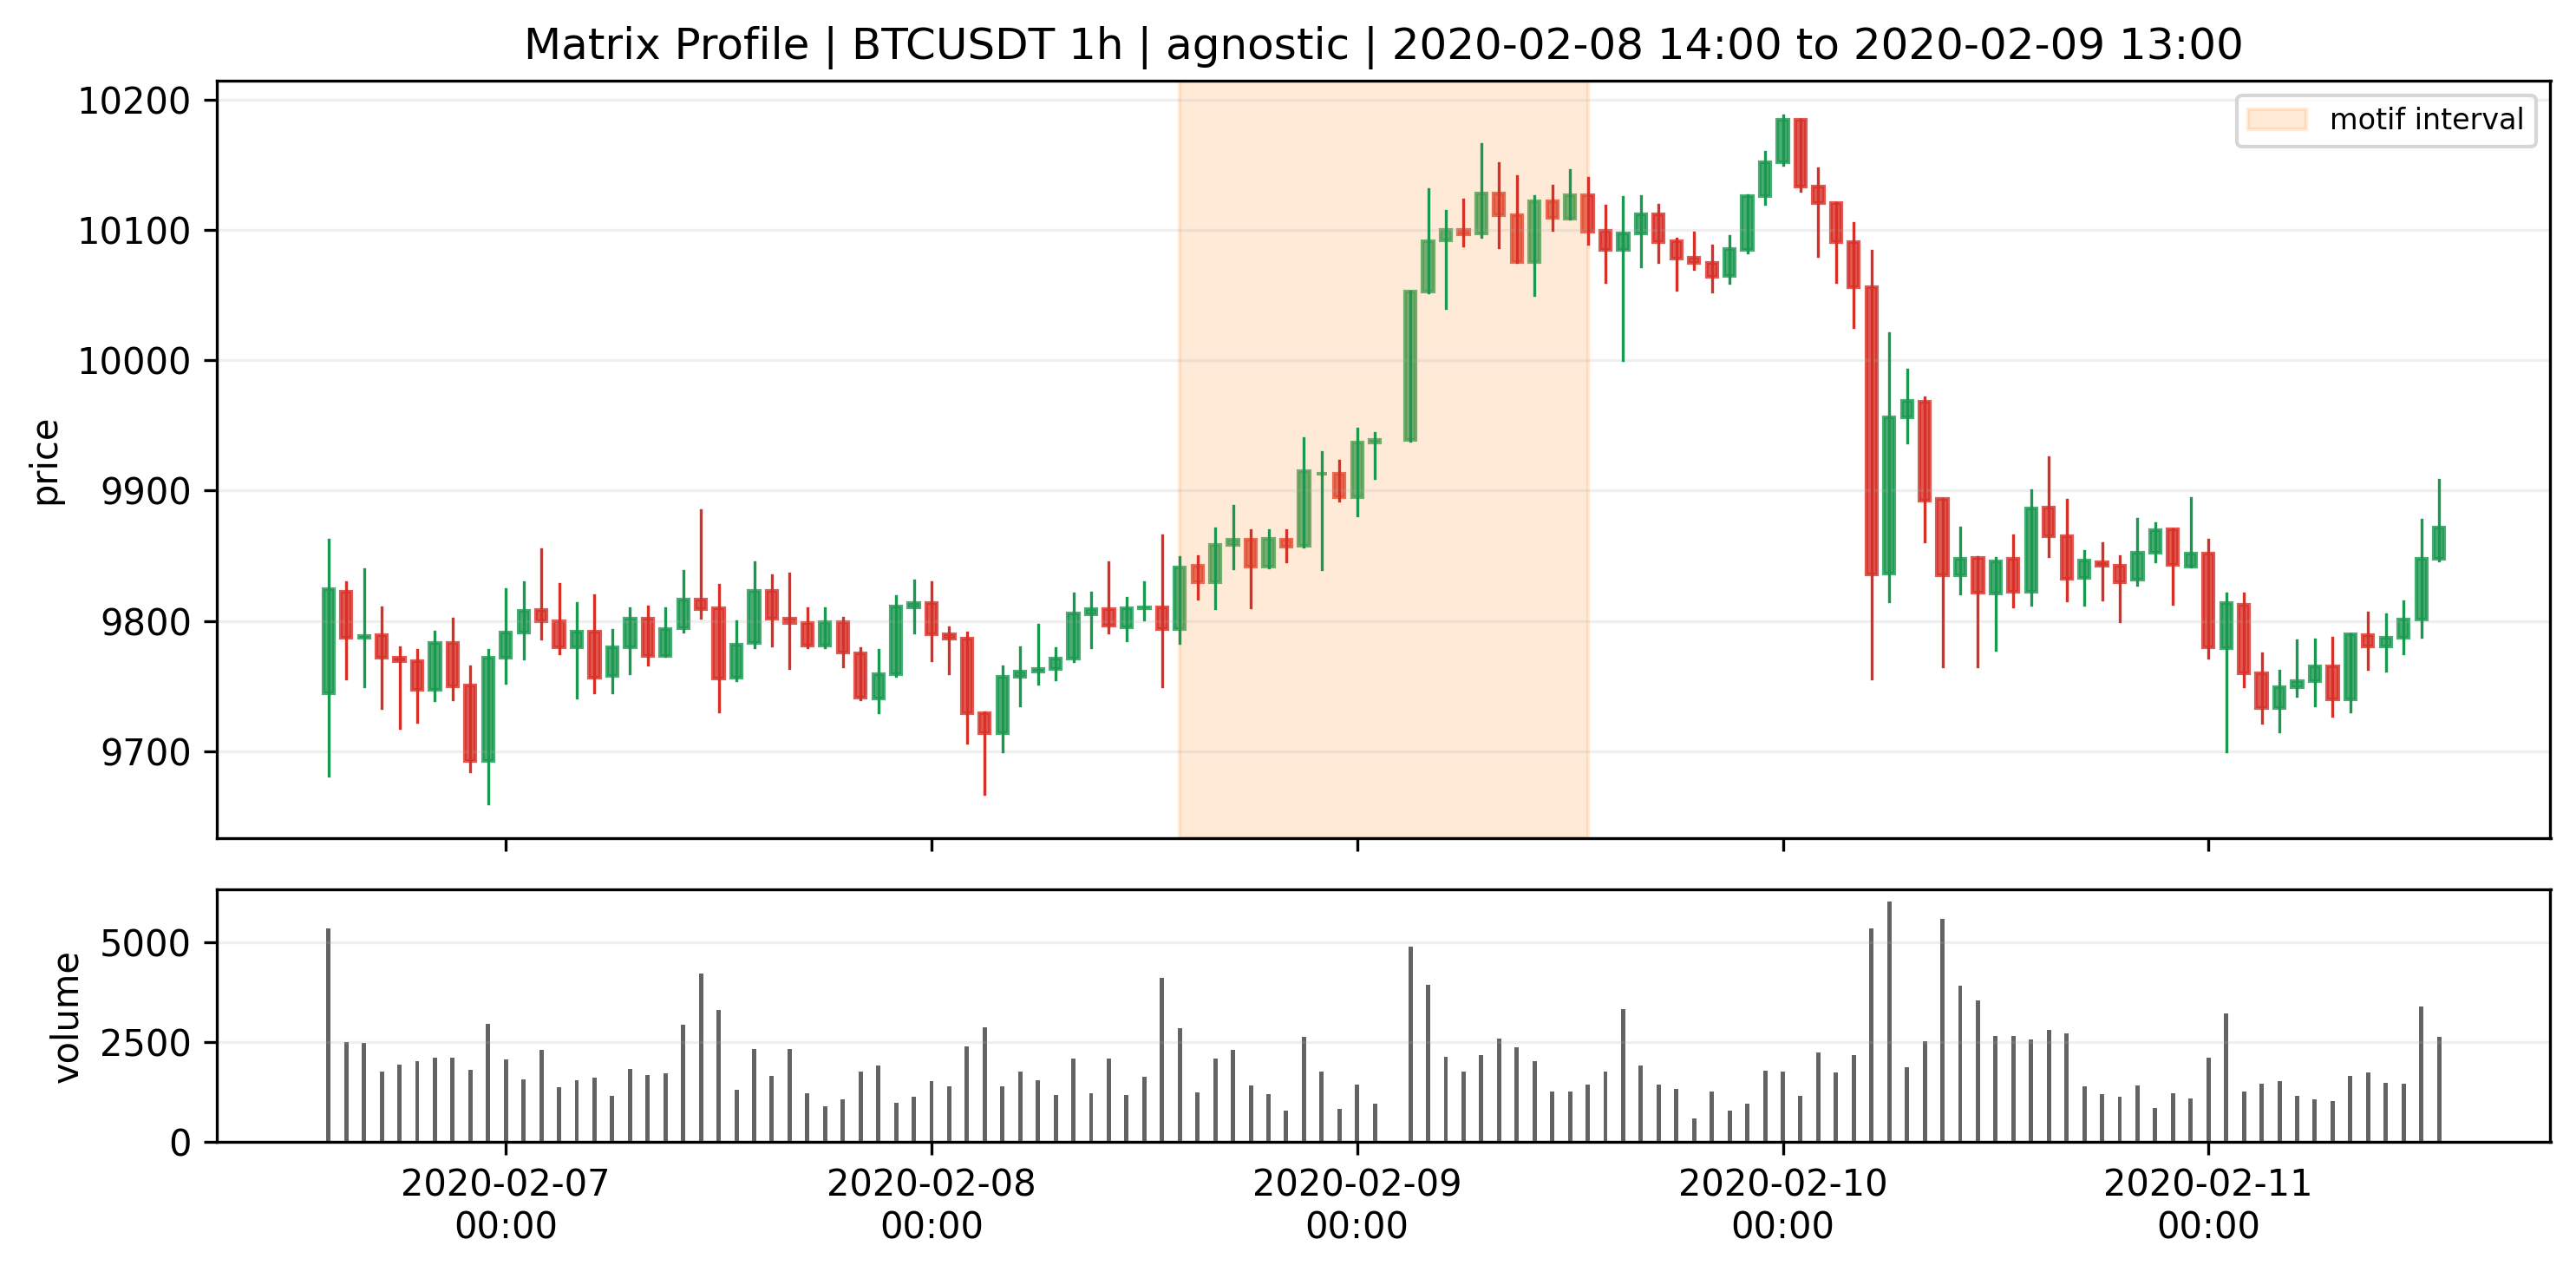
\includegraphics[width=0.9\linewidth]{reports/final_visual_evidence/figures/motif_17_matrix_profile_btcusdt_1h_agnostic_nan_pair1_1_context.png}
\caption{motif 17 matrix profile btcusdt 1h agnostic nan pair1 1 context. The shaded interval marks the discovered motif occurrence in original price context.}
\end{figure}

\begin{figure}[ht]
\centering
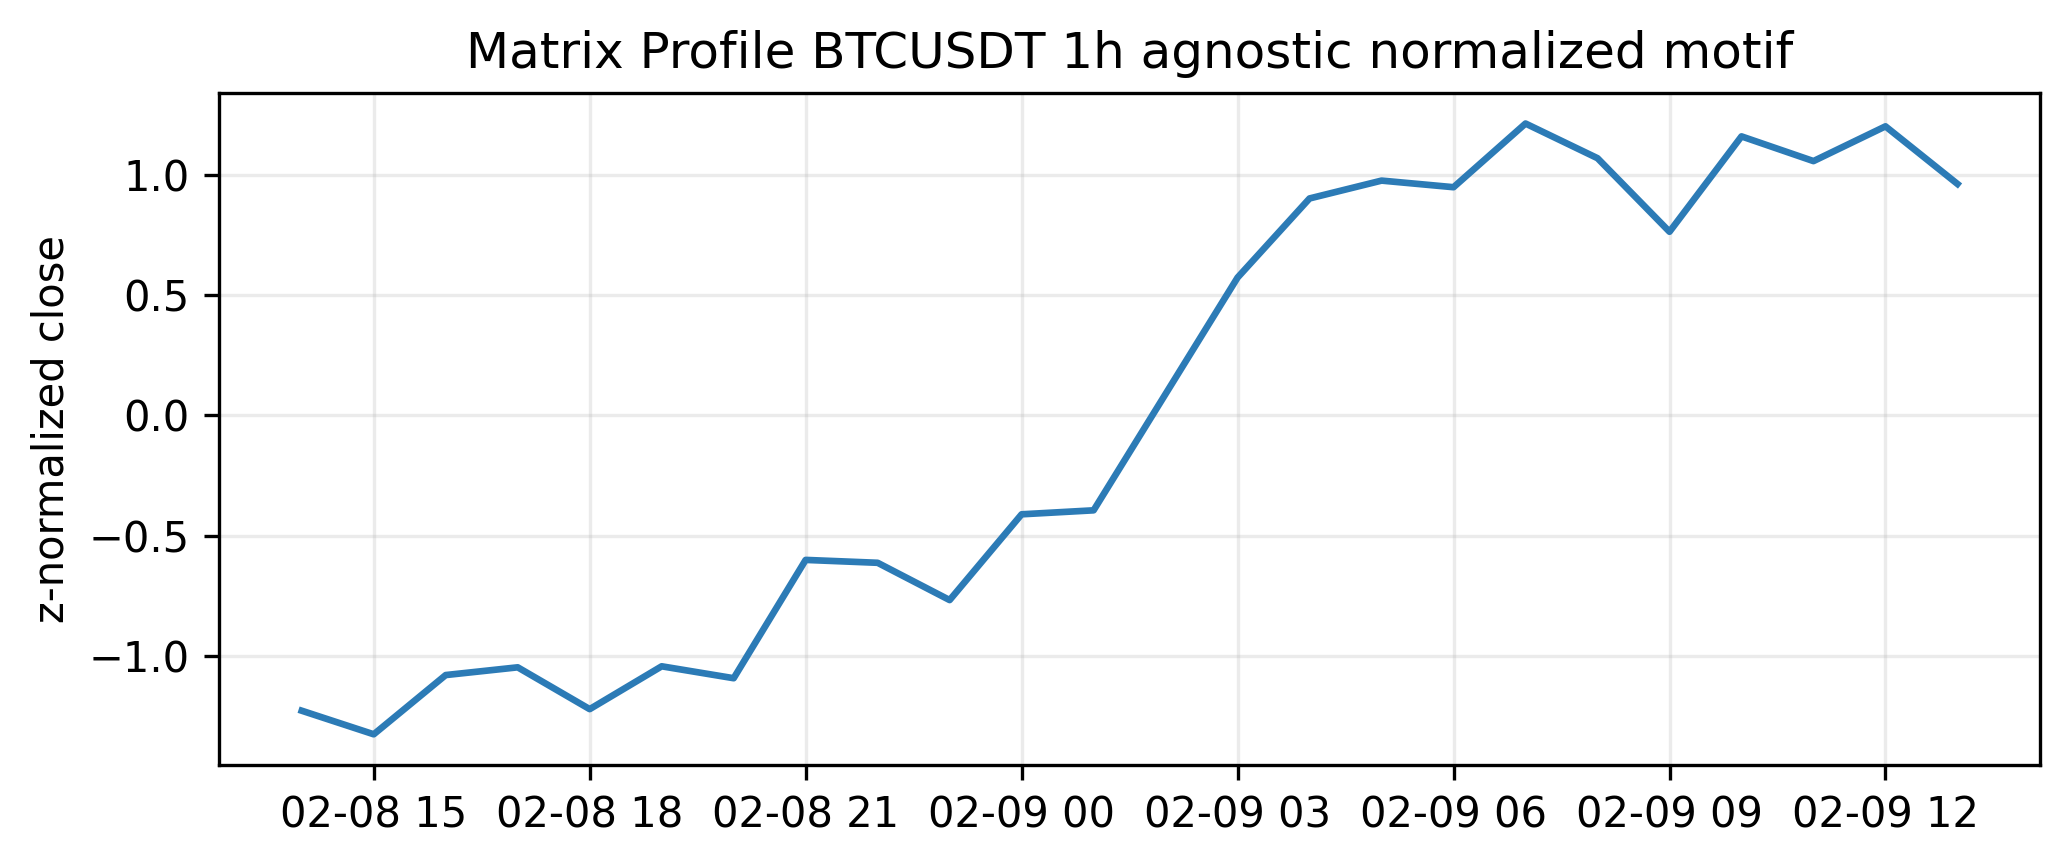
\includegraphics[width=0.9\linewidth]{reports/final_visual_evidence/figures/motif_17_matrix_profile_btcusdt_1h_agnostic_nan_pair1_1_normal_pattern.png}
\caption{motif 17 matrix profile btcusdt 1h agnostic nan pair1 1 normal pattern. The shaded interval marks the discovered motif occurrence in original price context.}
\end{figure}

\begin{figure}[ht]
\centering
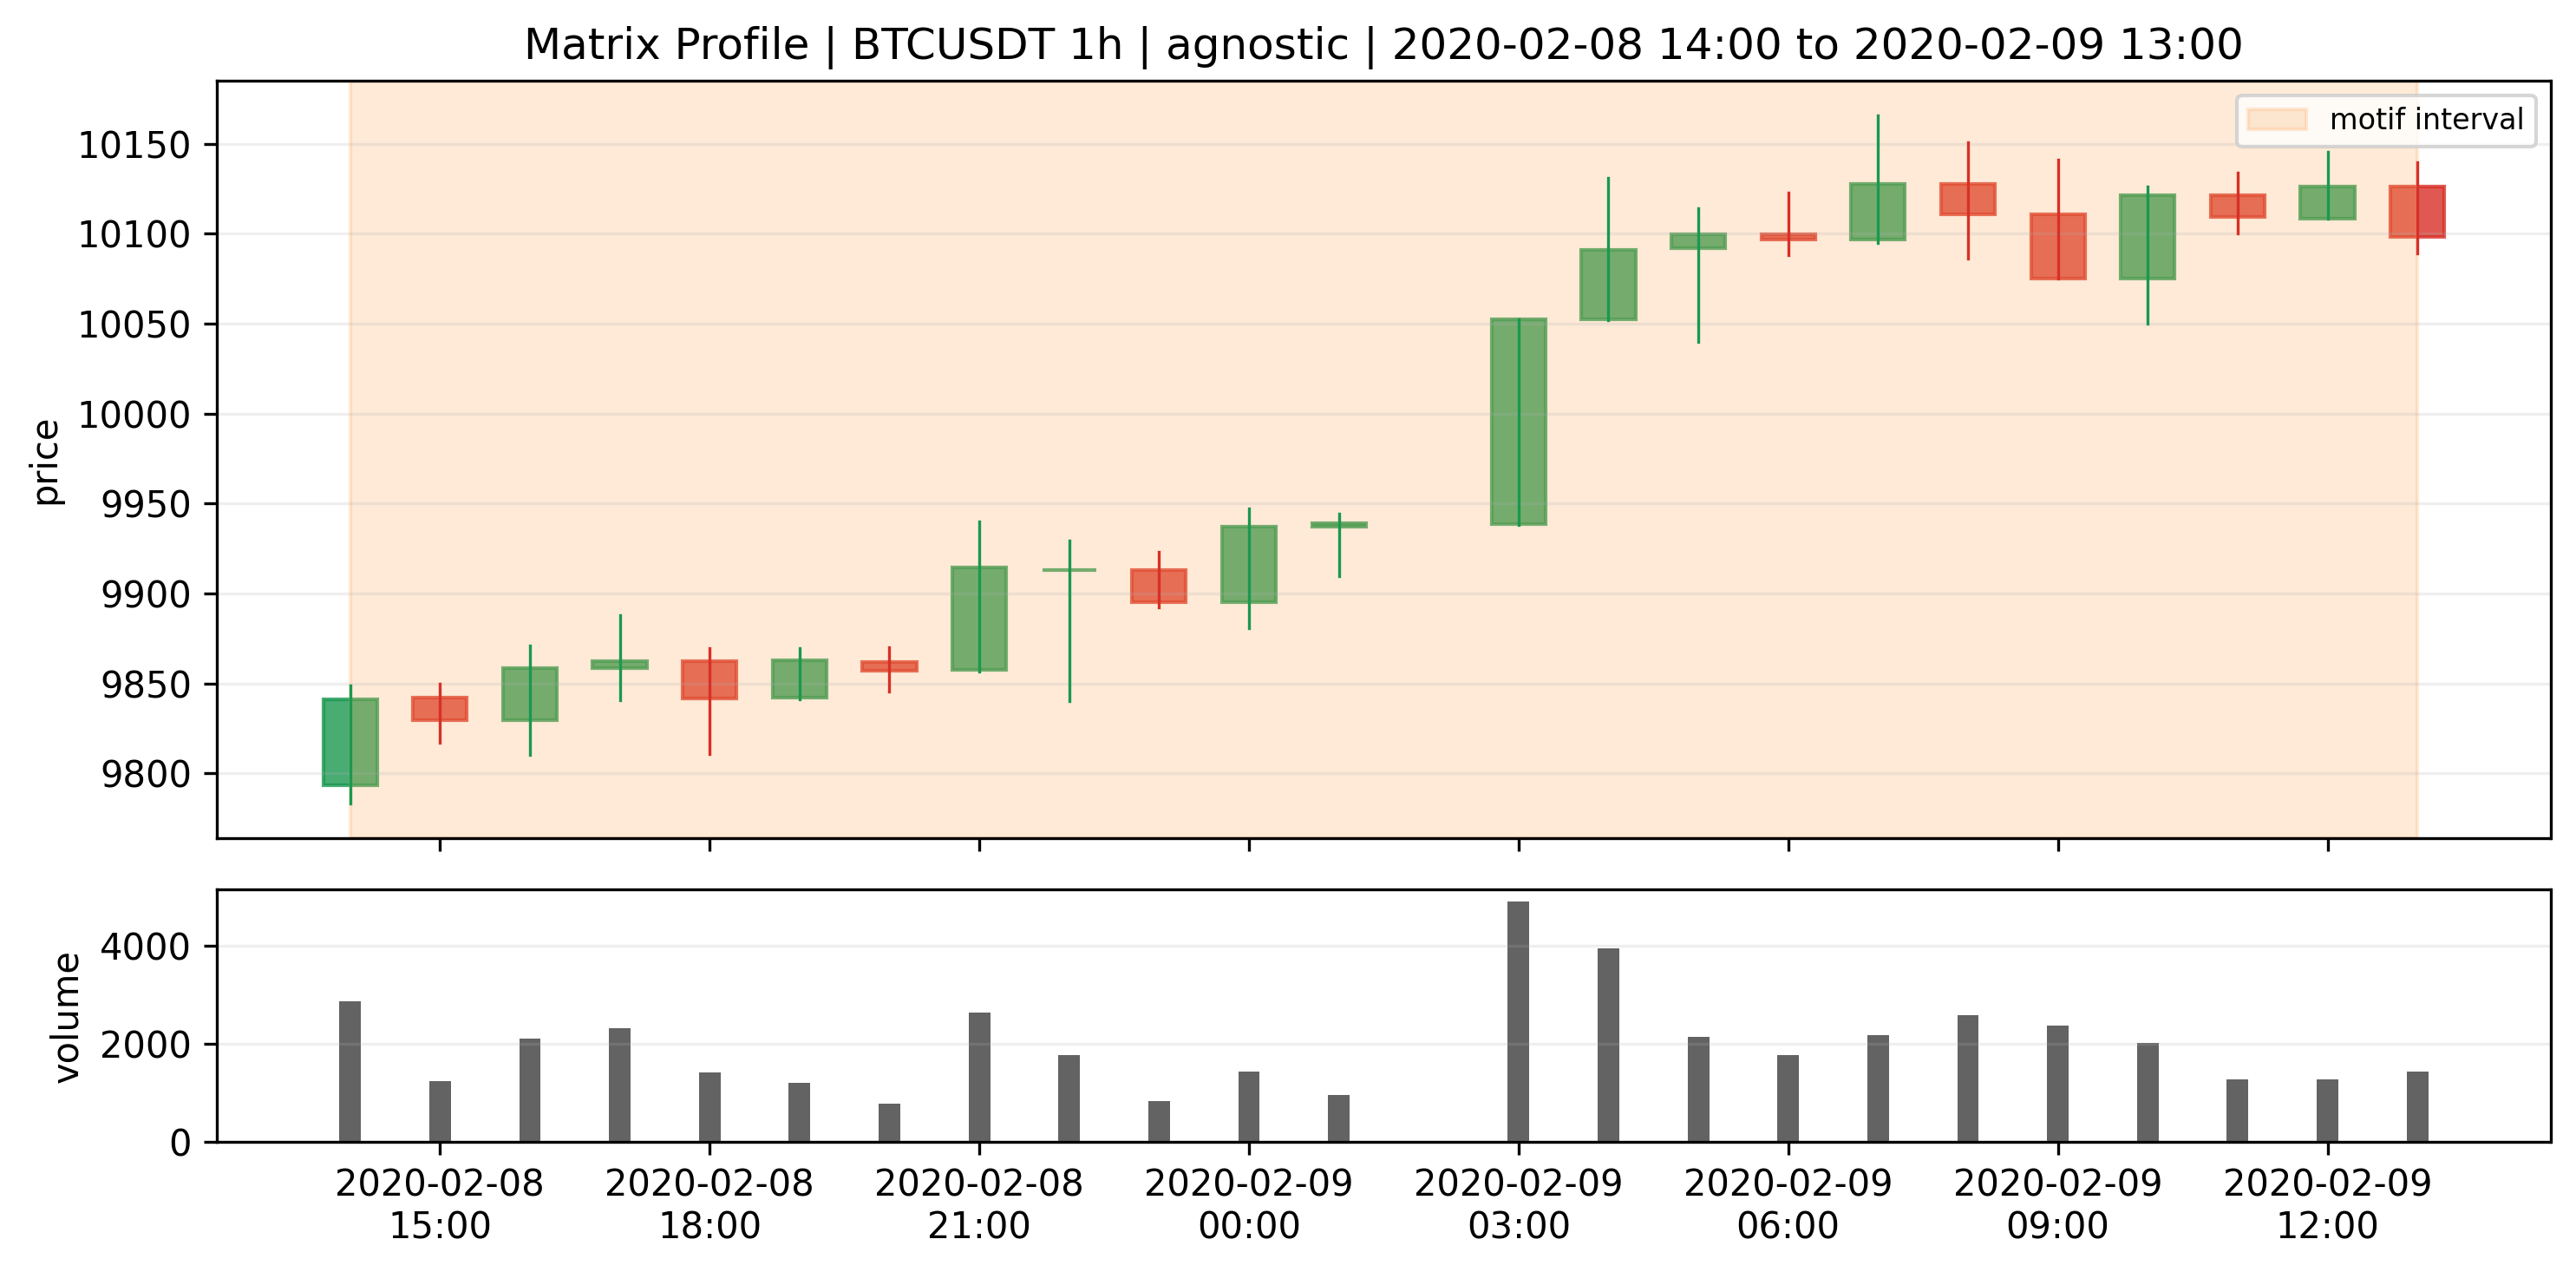
\includegraphics[width=0.9\linewidth]{reports/final_visual_evidence/figures/motif_17_matrix_profile_btcusdt_1h_agnostic_nan_pair1_1_zoom.png}
\caption{motif 17 matrix profile btcusdt 1h agnostic nan pair1 1 zoom. The shaded interval marks the discovered motif occurrence in original price context.}
\end{figure}

\begin{figure}[ht]
\centering
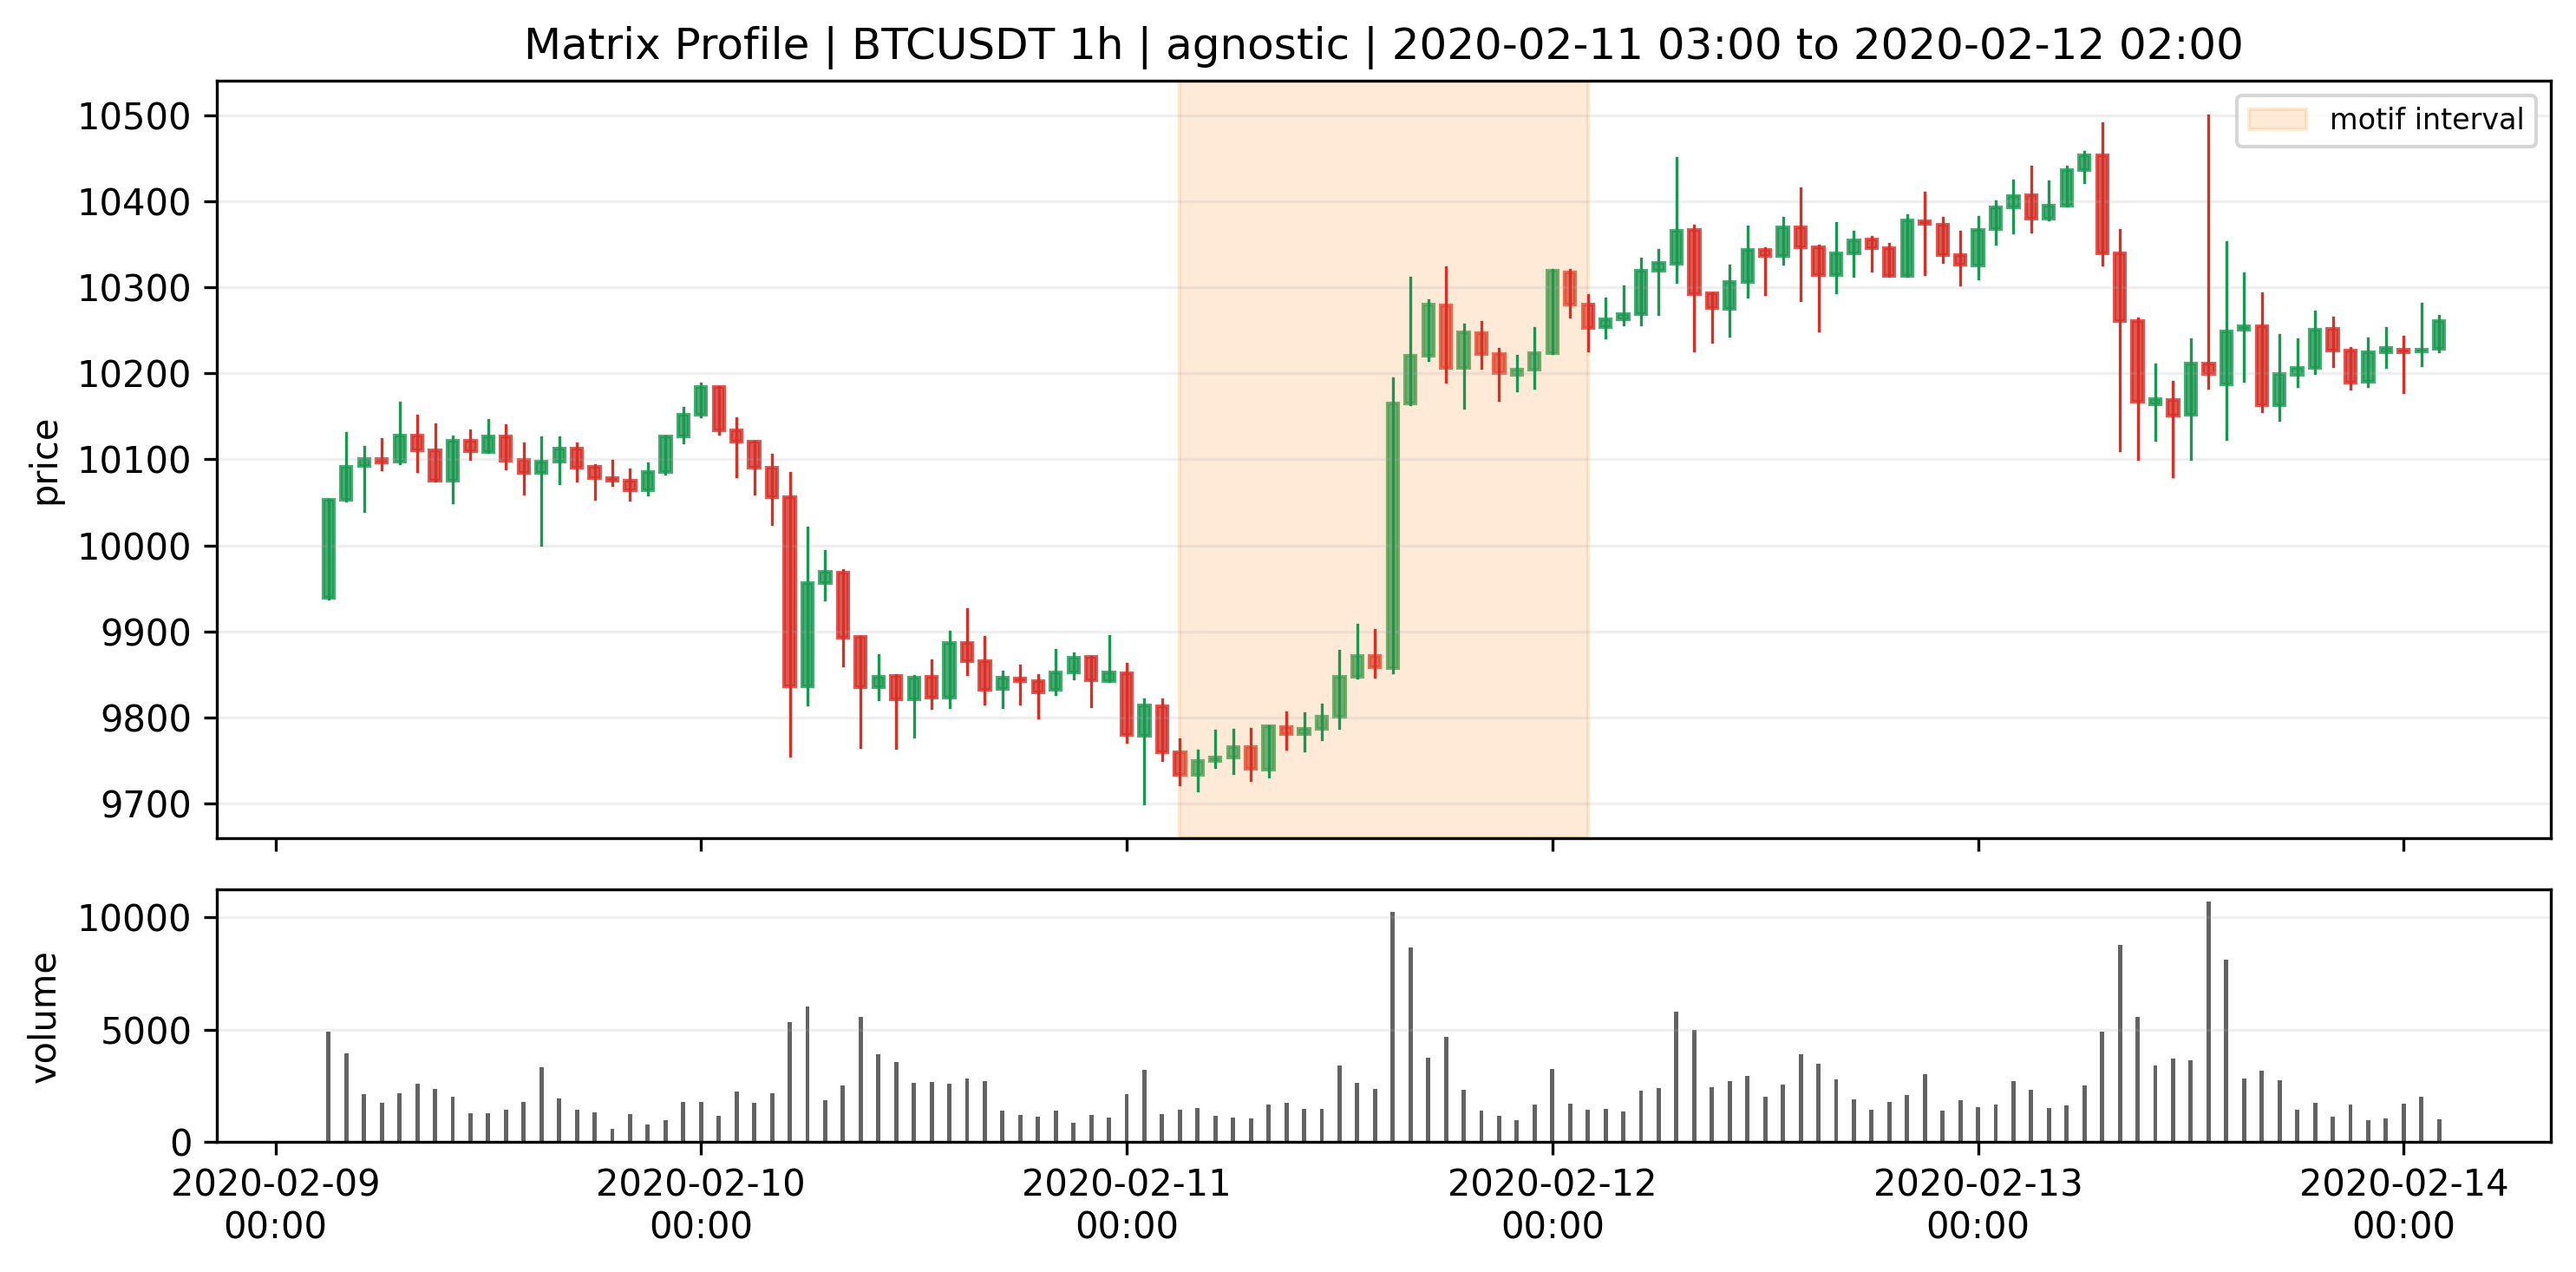
\includegraphics[width=0.9\linewidth]{reports/final_visual_evidence/figures/motif_18_matrix_profile_btcusdt_1h_agnostic_nan_pair1_2_context.png}
\caption{motif 18 matrix profile btcusdt 1h agnostic nan pair1 2 context. The shaded interval marks the discovered motif occurrence in original price context.}
\end{figure}

\begin{figure}[ht]
\centering
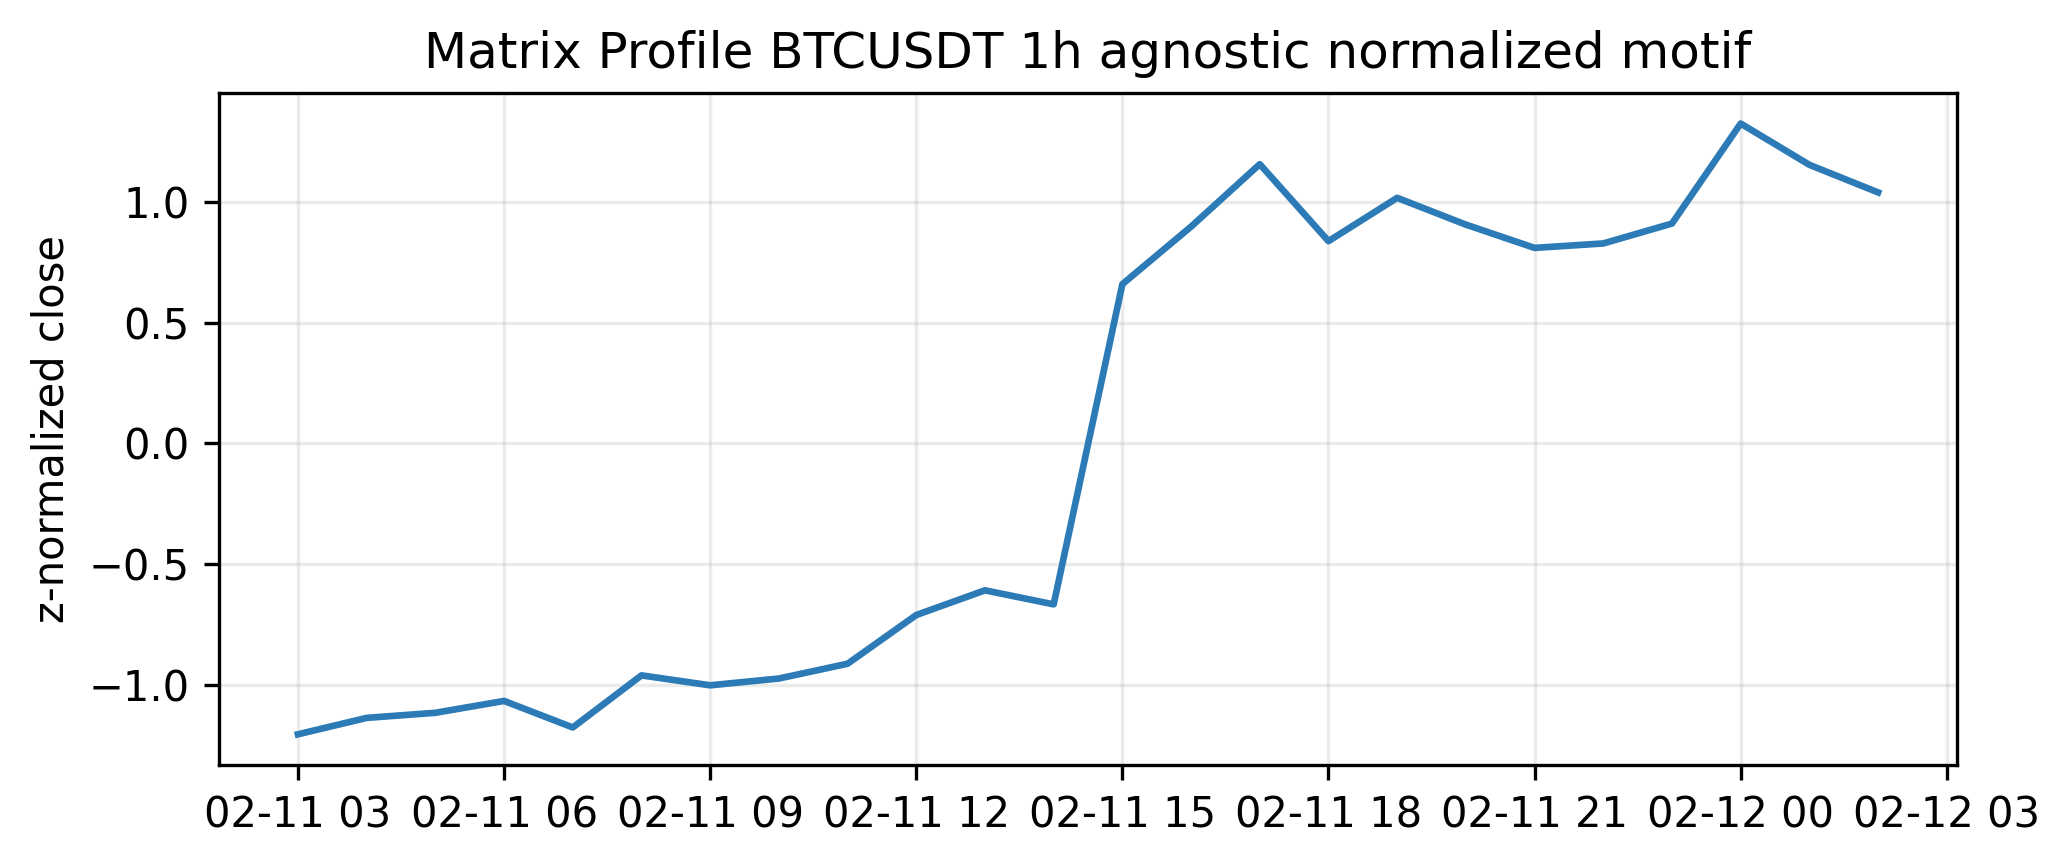
\includegraphics[width=0.9\linewidth]{reports/final_visual_evidence/figures/motif_18_matrix_profile_btcusdt_1h_agnostic_nan_pair1_2_normal_pattern.png}
\caption{motif 18 matrix profile btcusdt 1h agnostic nan pair1 2 normal pattern. The shaded interval marks the discovered motif occurrence in original price context.}
\end{figure}

\begin{figure}[ht]
\centering
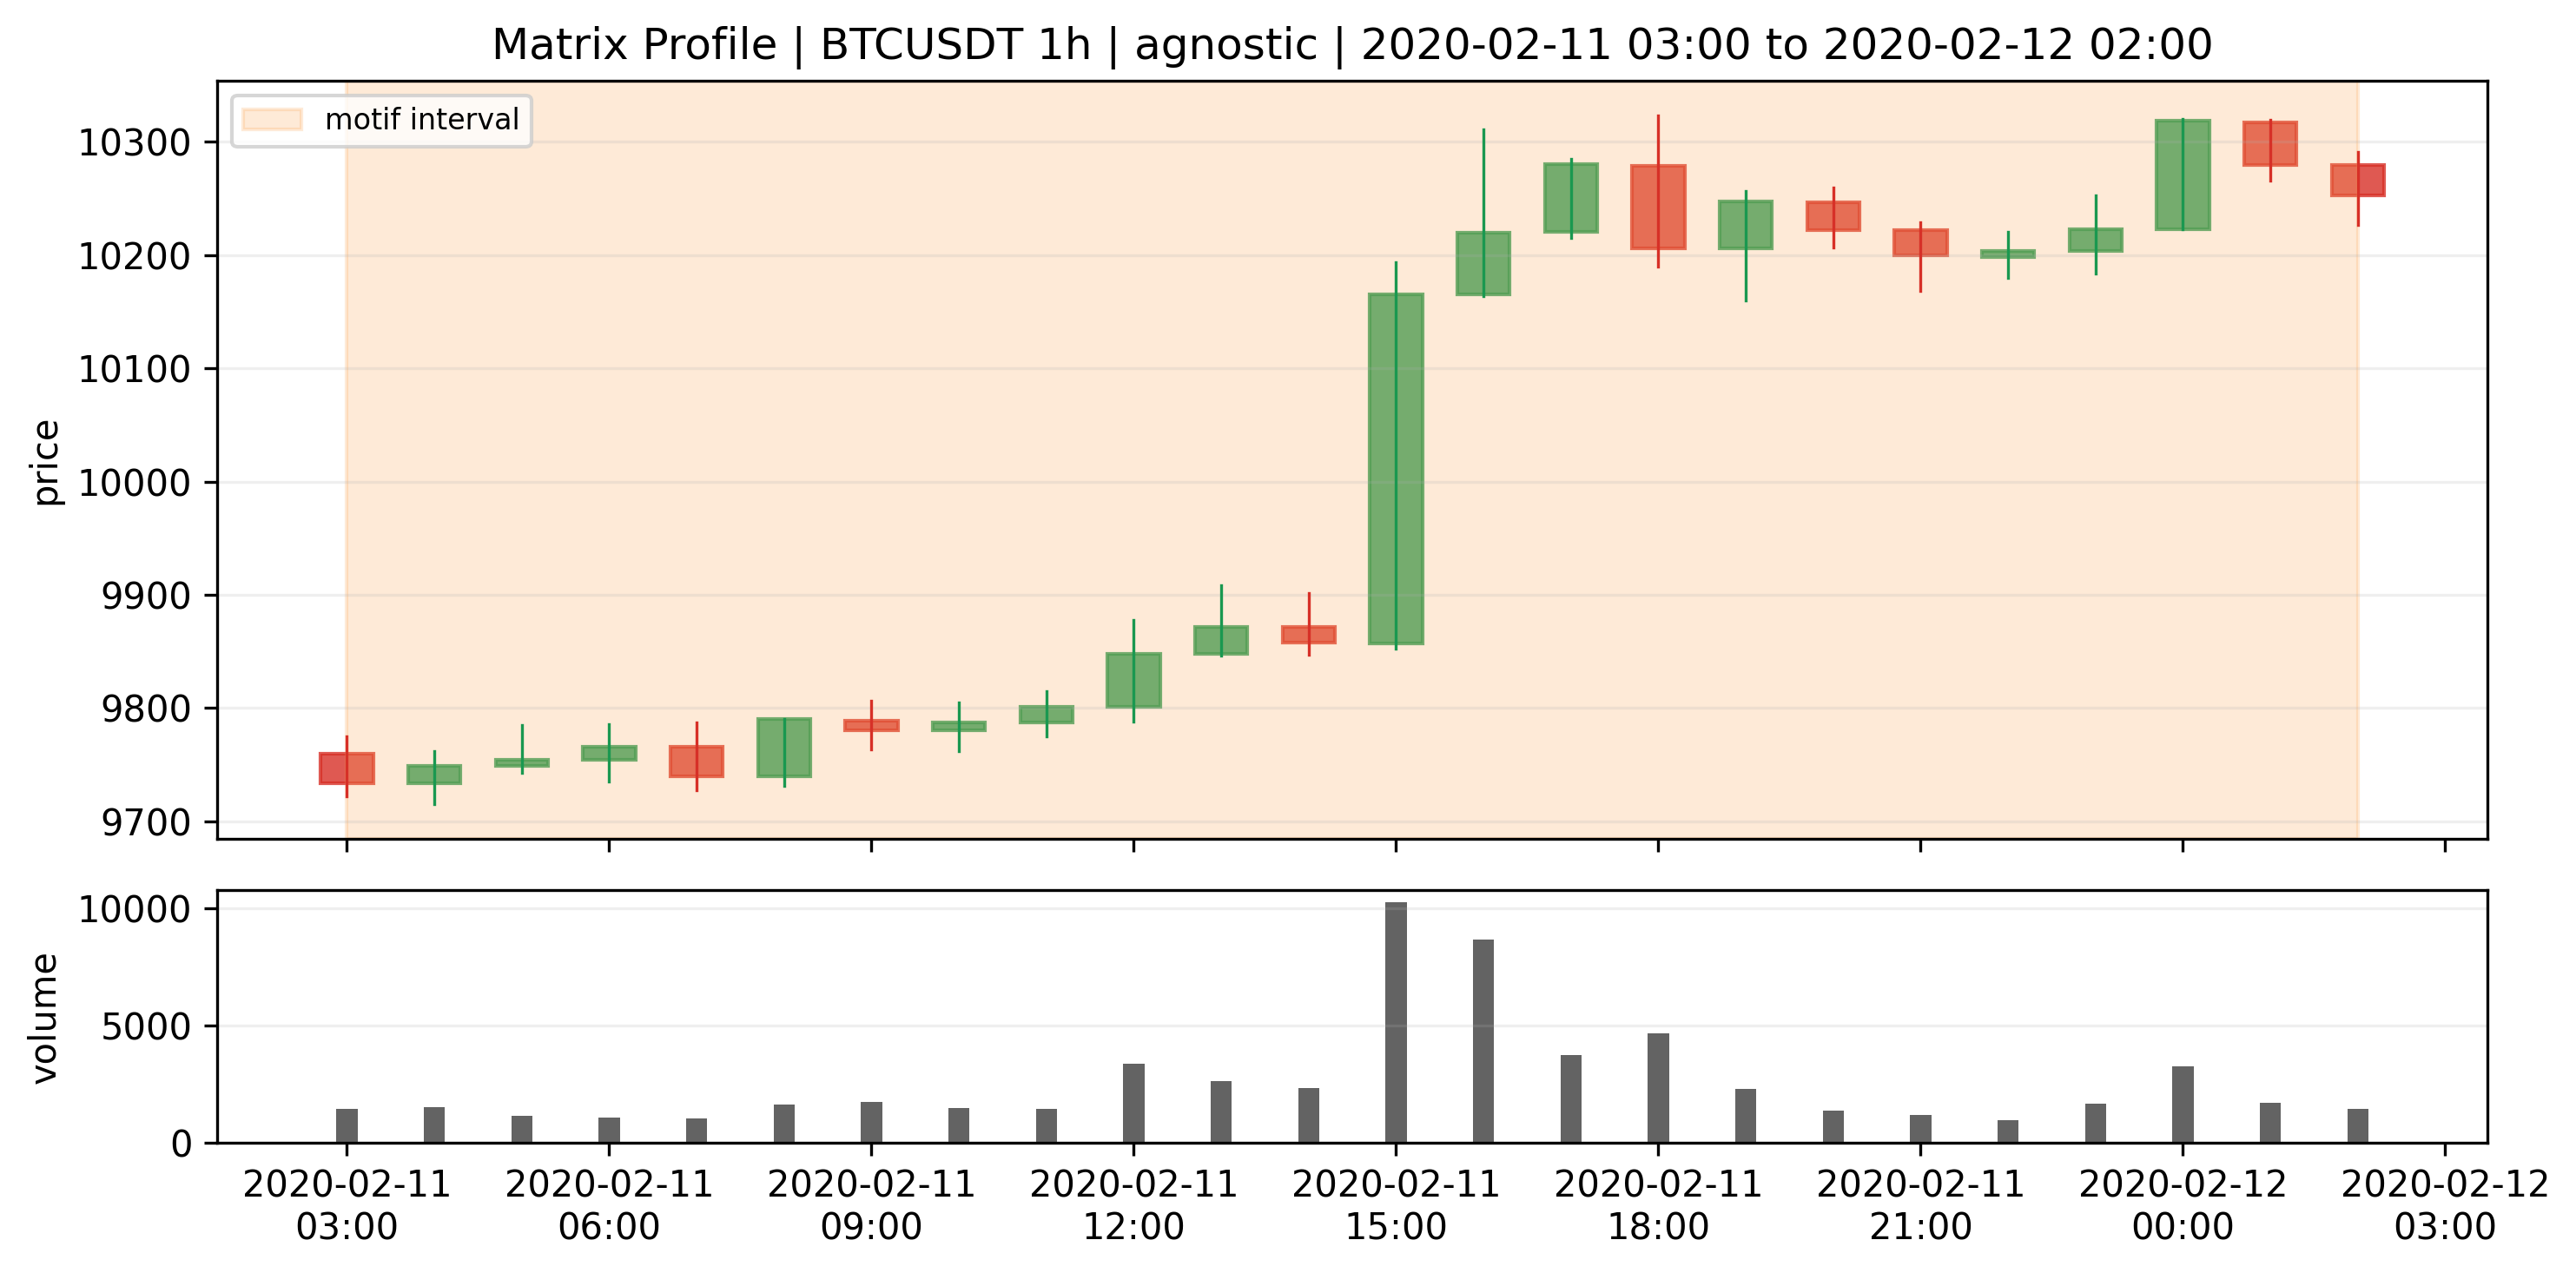
\includegraphics[width=0.9\linewidth]{reports/final_visual_evidence/figures/motif_18_matrix_profile_btcusdt_1h_agnostic_nan_pair1_2_zoom.png}
\caption{motif 18 matrix profile btcusdt 1h agnostic nan pair1 2 zoom. The shaded interval marks the discovered motif occurrence in original price context.}
\end{figure}

\begin{figure}[ht]
\centering
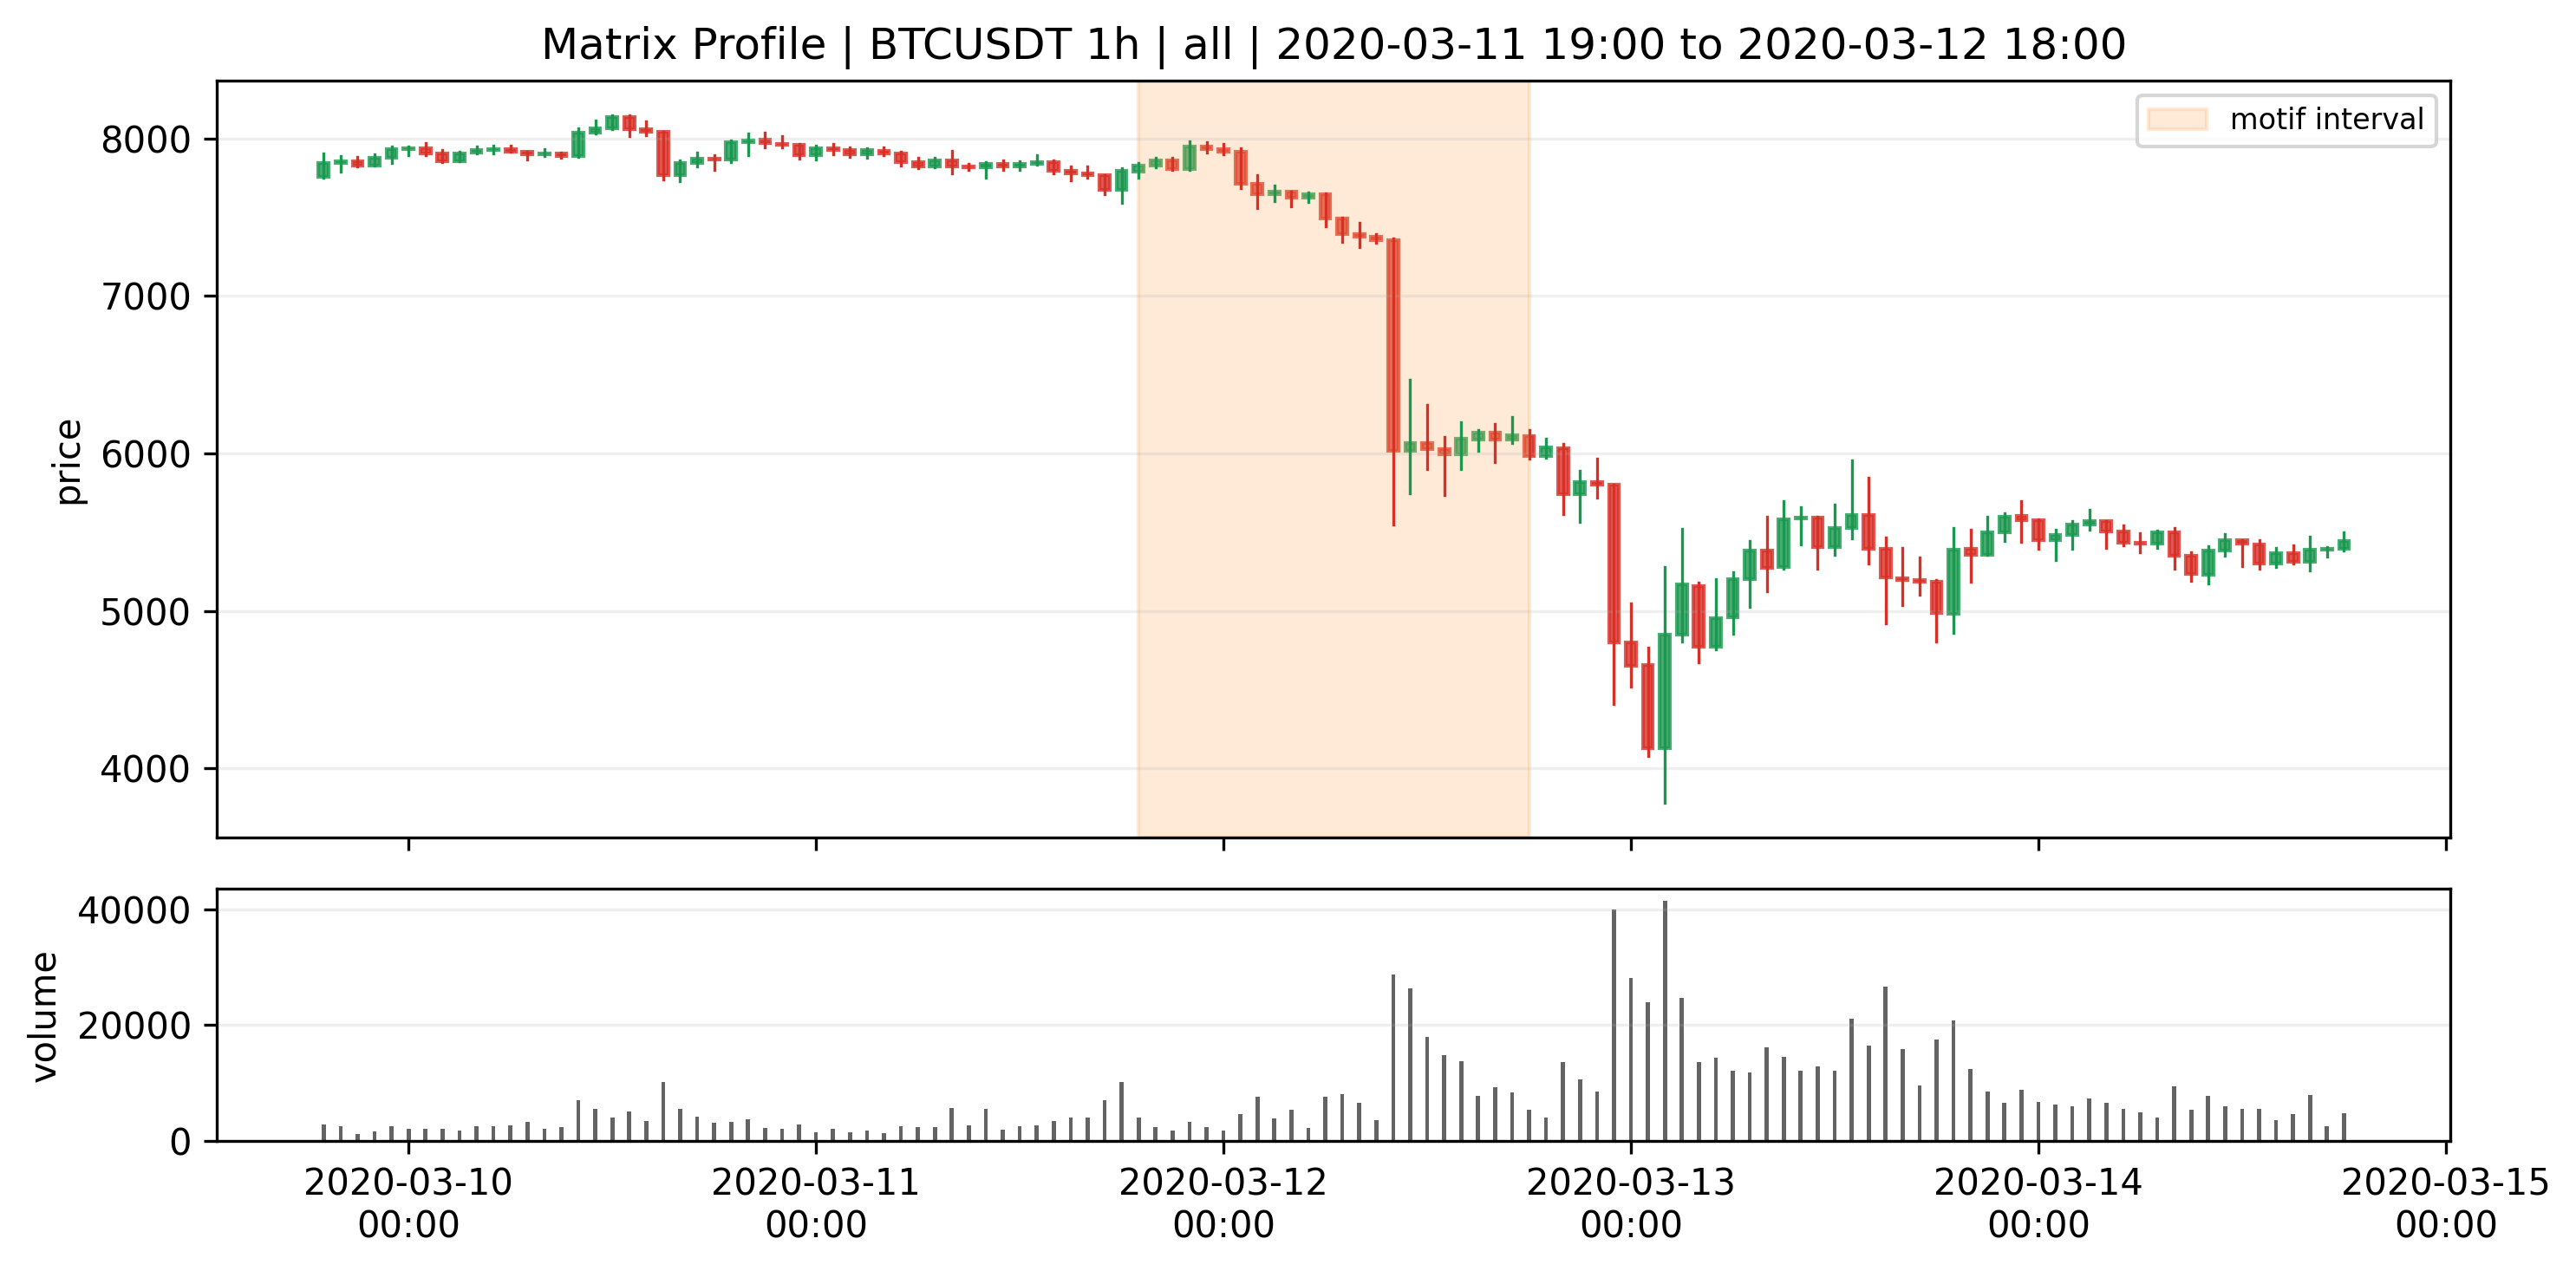
\includegraphics[width=0.9\linewidth]{reports/final_visual_evidence/figures/motif_19_matrix_profile_btcusdt_1h_all_1_0_pair19_1_context.png}
\caption{motif 19 matrix profile btcusdt 1h all 1 0 pair19 1 context. The shaded interval marks the discovered motif occurrence in original price context.}
\end{figure}

\begin{figure}[ht]
\centering
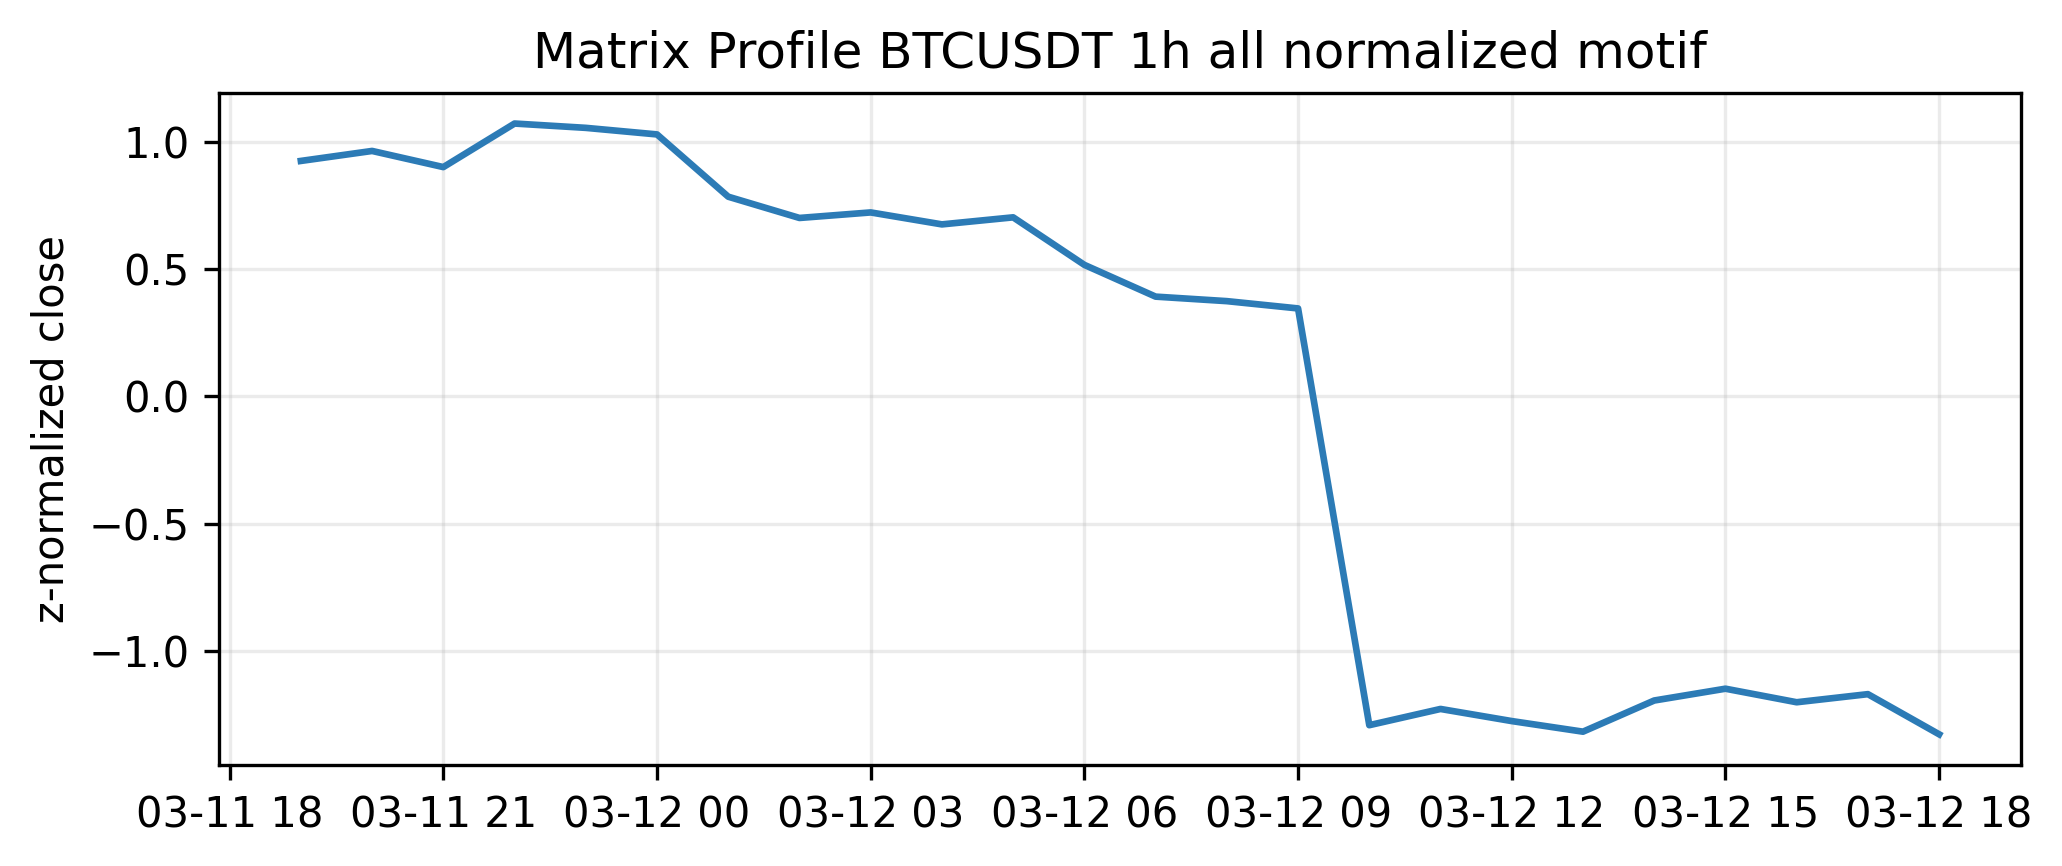
\includegraphics[width=0.9\linewidth]{reports/final_visual_evidence/figures/motif_19_matrix_profile_btcusdt_1h_all_1_0_pair19_1_normal_pattern.png}
\caption{motif 19 matrix profile btcusdt 1h all 1 0 pair19 1 normal pattern. The shaded interval marks the discovered motif occurrence in original price context.}
\end{figure}

\begin{figure}[ht]
\centering
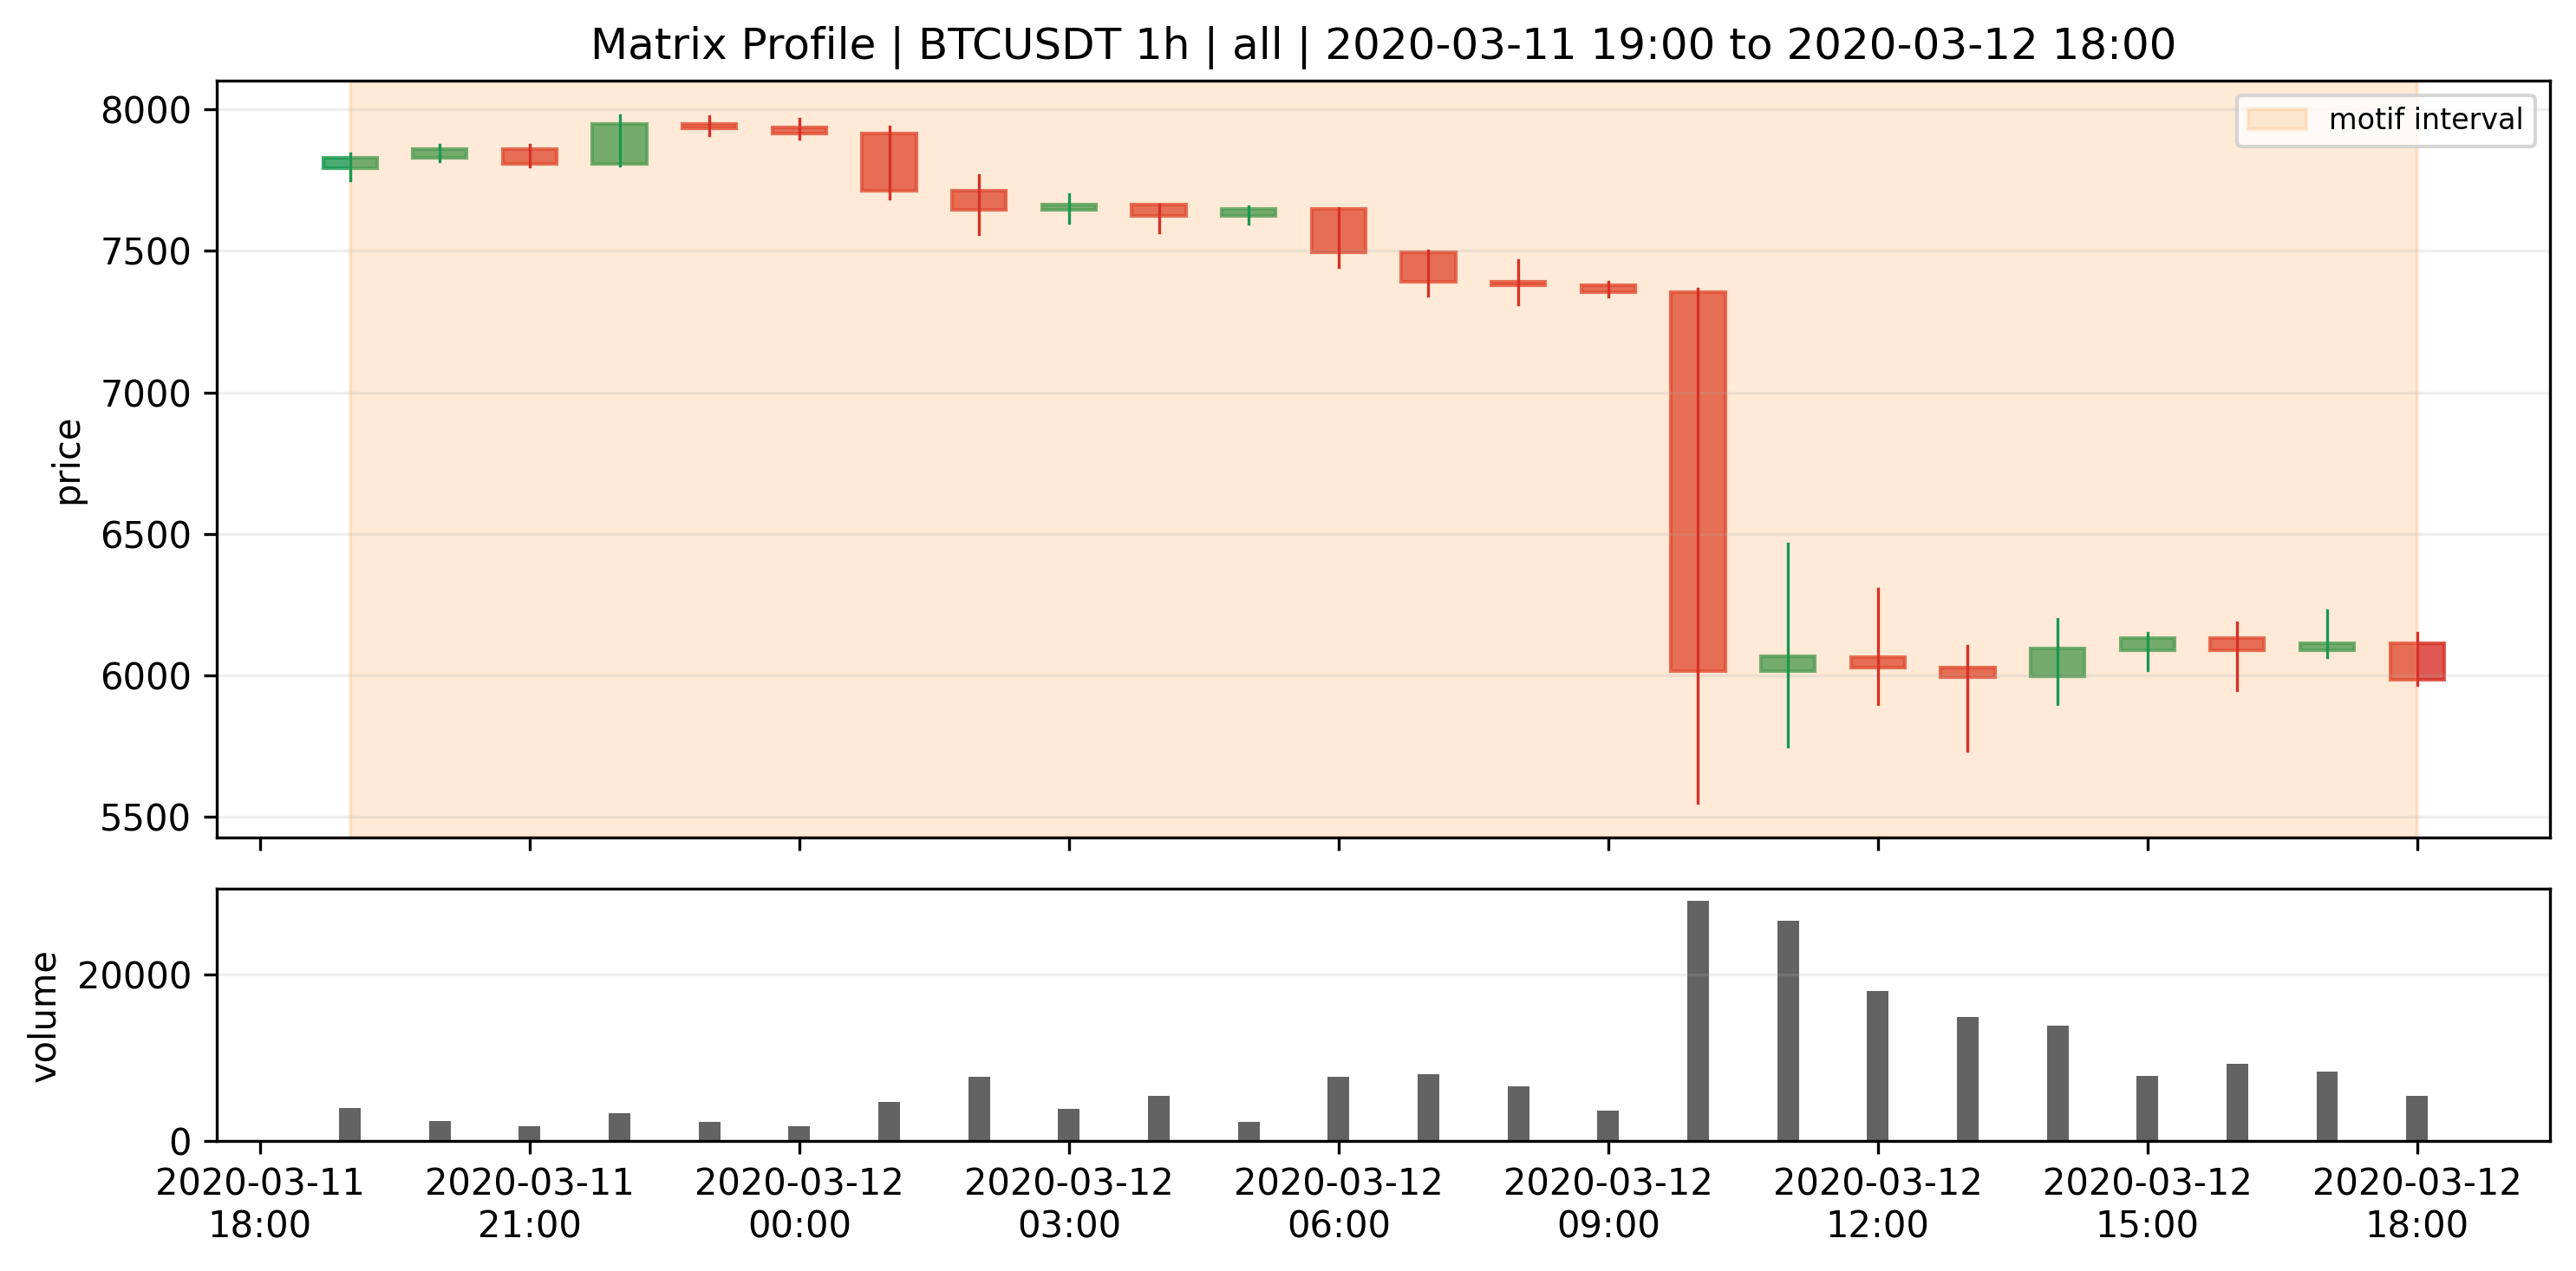
\includegraphics[width=0.9\linewidth]{reports/final_visual_evidence/figures/motif_19_matrix_profile_btcusdt_1h_all_1_0_pair19_1_zoom.png}
\caption{motif 19 matrix profile btcusdt 1h all 1 0 pair19 1 zoom. The shaded interval marks the discovered motif occurrence in original price context.}
\end{figure}

\begin{figure}[ht]
\centering
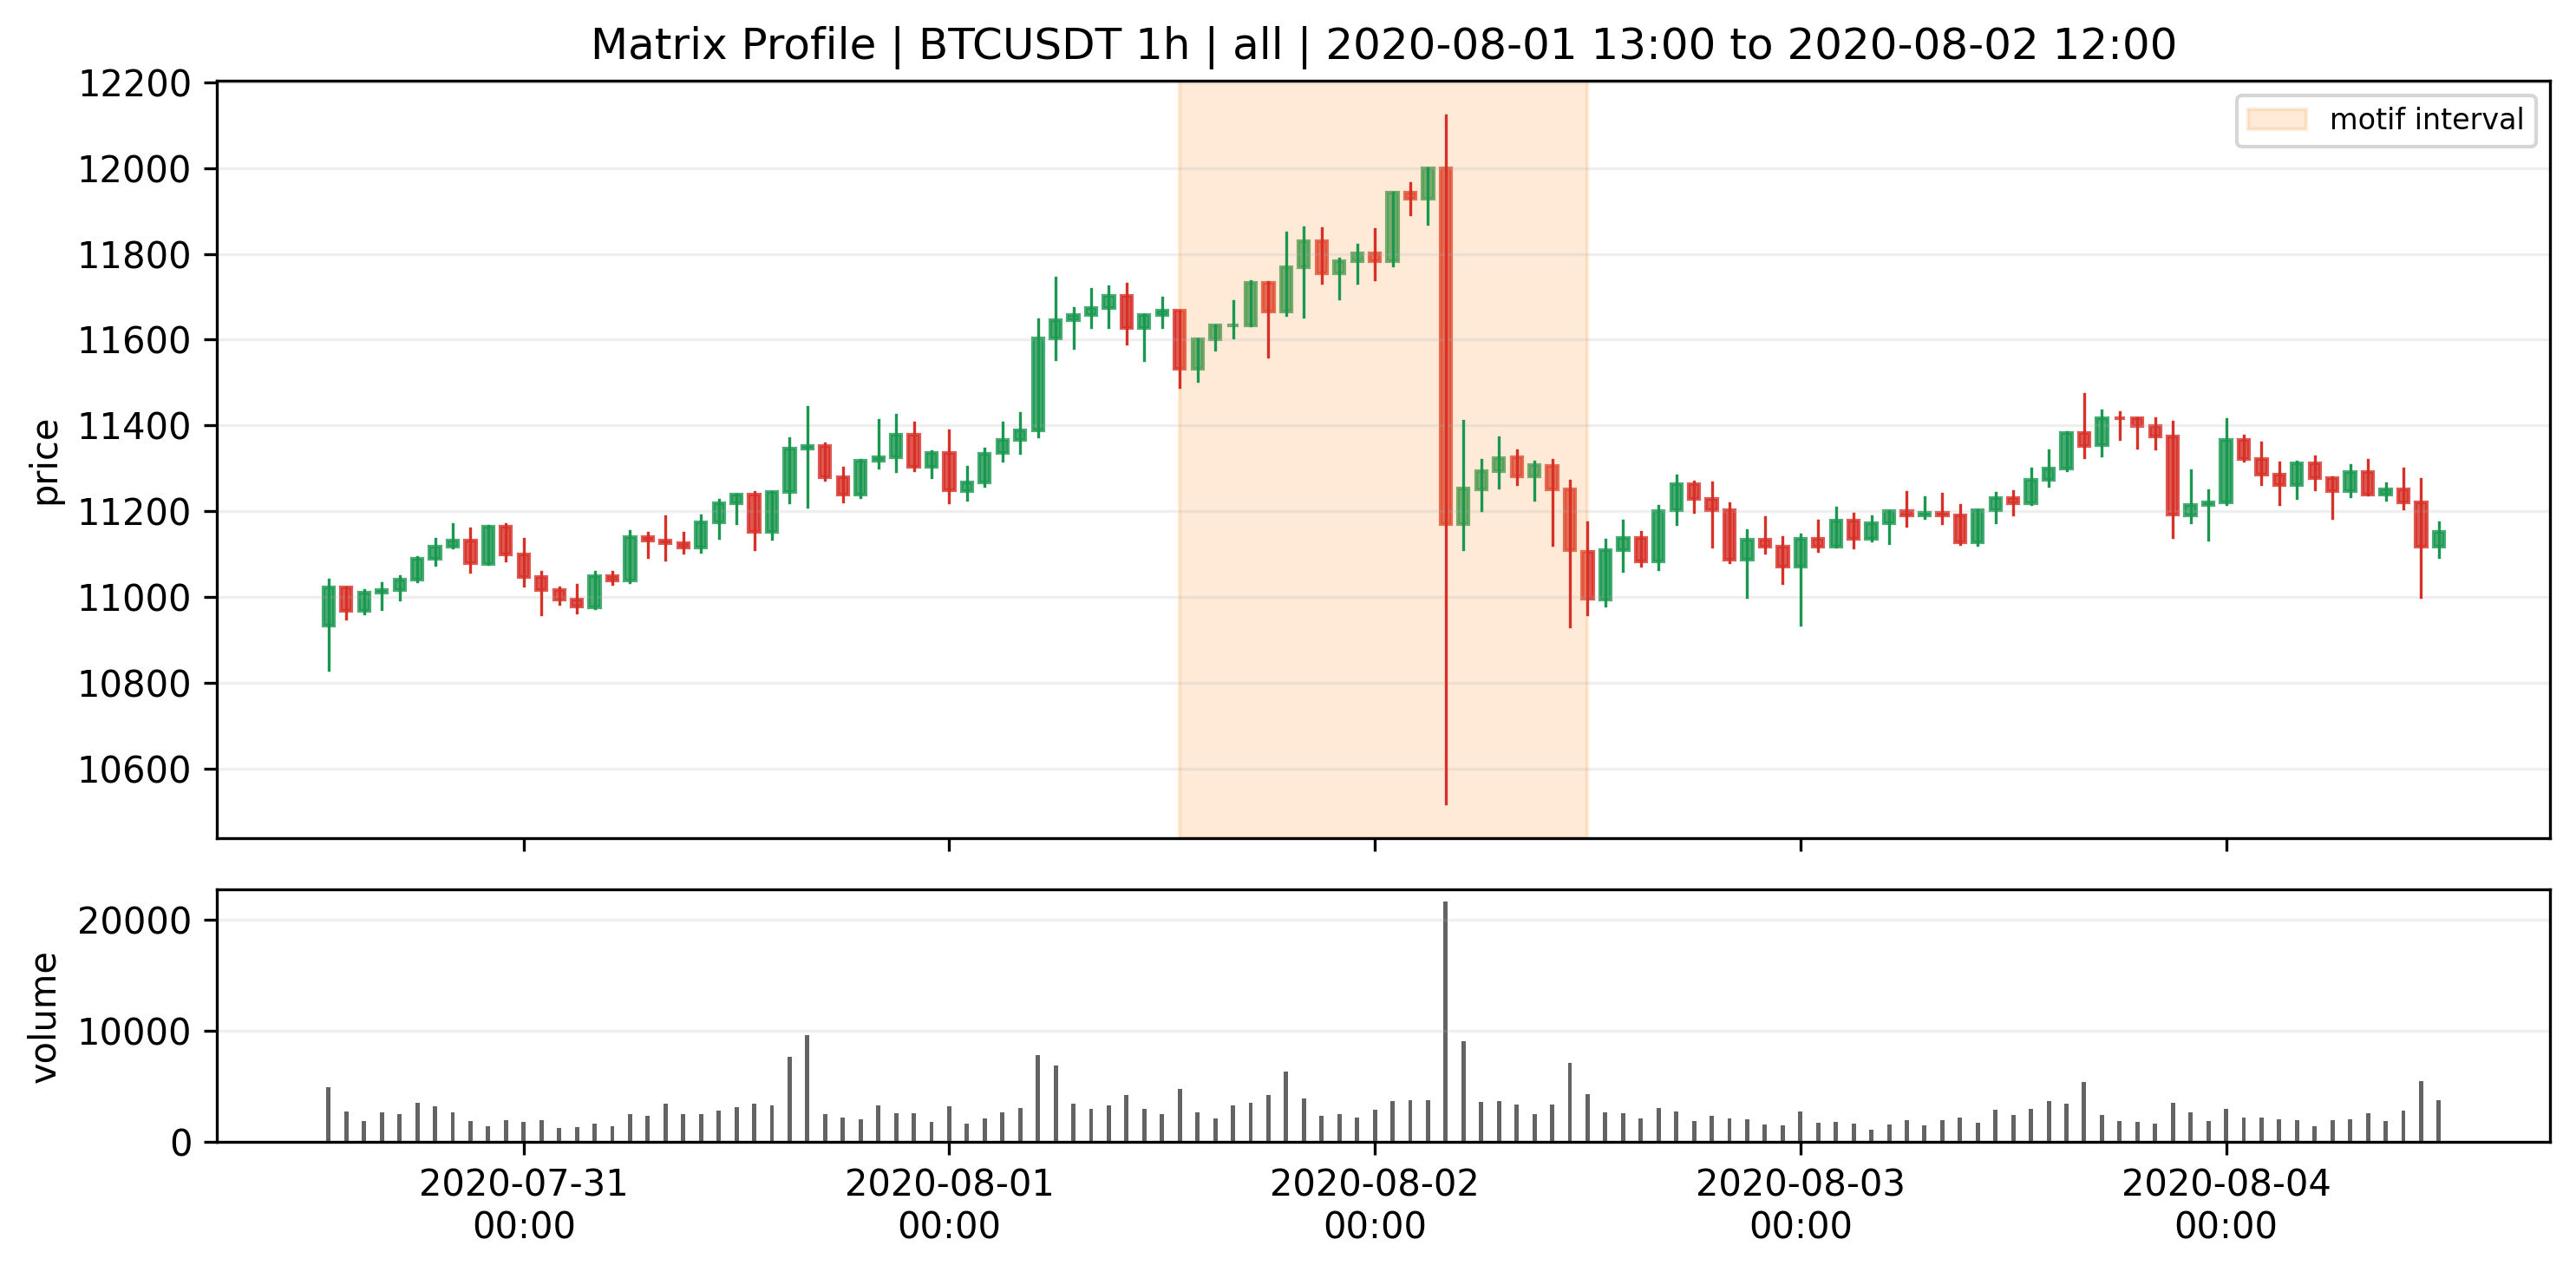
\includegraphics[width=0.9\linewidth]{reports/final_visual_evidence/figures/motif_20_matrix_profile_btcusdt_1h_all_1_0_pair19_2_context.png}
\caption{motif 20 matrix profile btcusdt 1h all 1 0 pair19 2 context. The shaded interval marks the discovered motif occurrence in original price context.}
\end{figure}

\begin{figure}[ht]
\centering
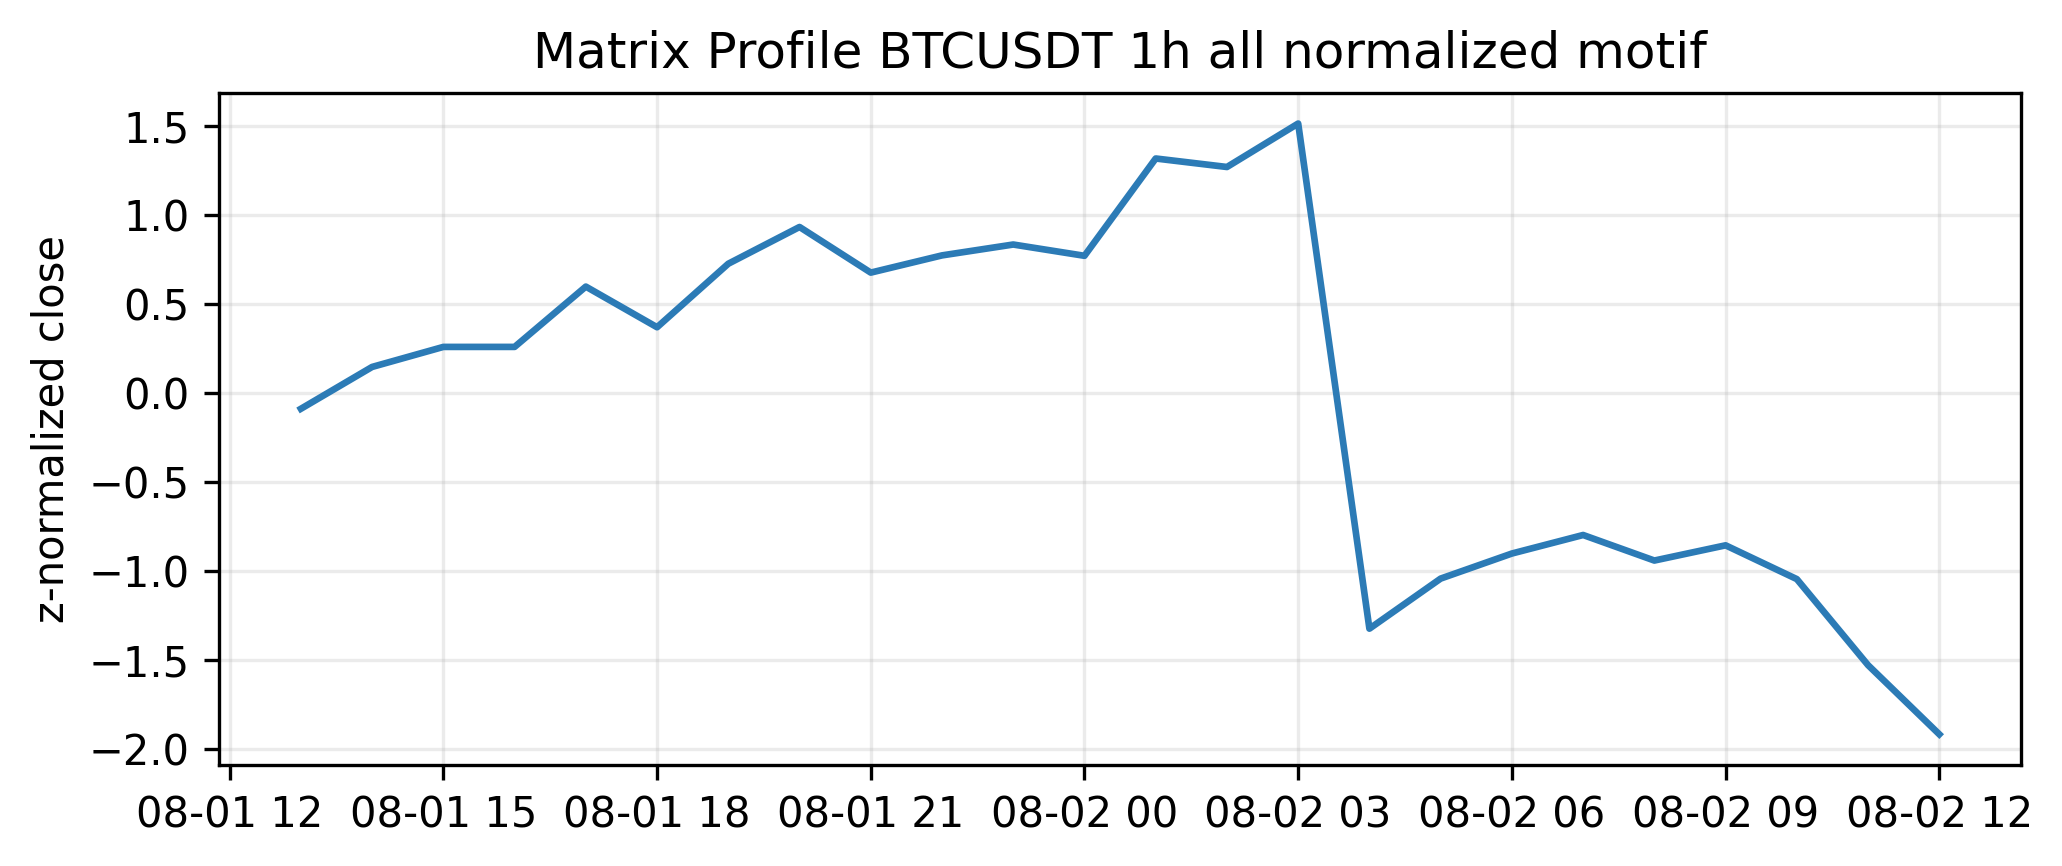
\includegraphics[width=0.9\linewidth]{reports/final_visual_evidence/figures/motif_20_matrix_profile_btcusdt_1h_all_1_0_pair19_2_normal_pattern.png}
\caption{motif 20 matrix profile btcusdt 1h all 1 0 pair19 2 normal pattern. The shaded interval marks the discovered motif occurrence in original price context.}
\end{figure}

\begin{figure}[ht]
\centering
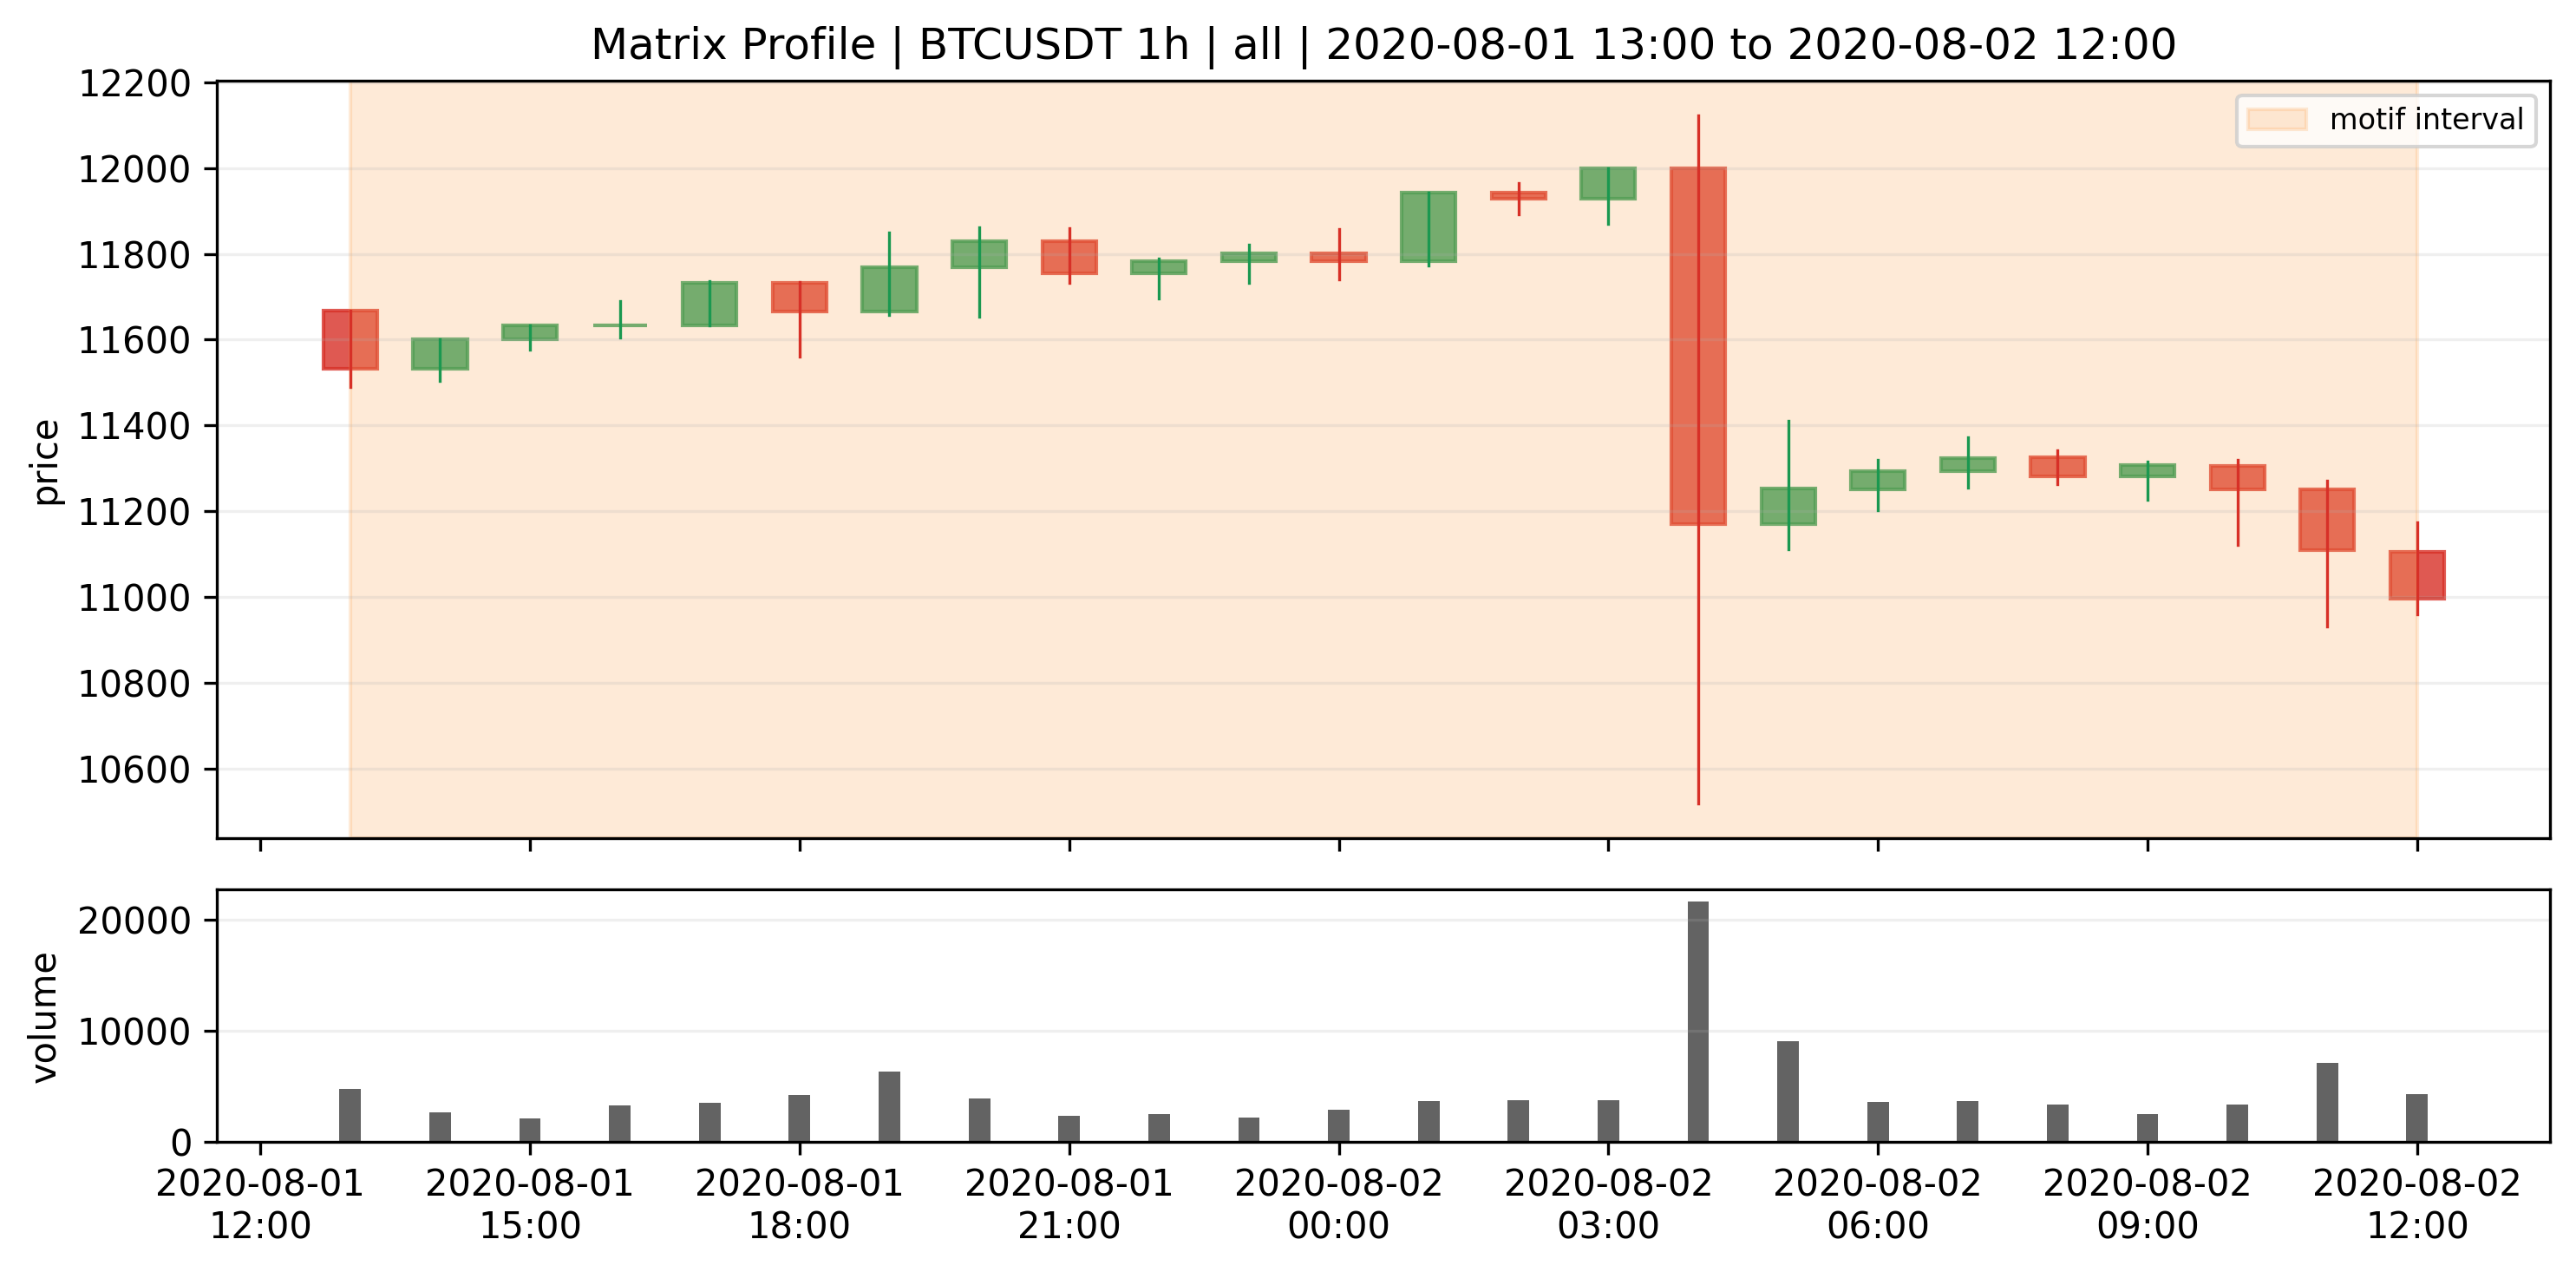
\includegraphics[width=0.9\linewidth]{reports/final_visual_evidence/figures/motif_20_matrix_profile_btcusdt_1h_all_1_0_pair19_2_zoom.png}
\caption{motif 20 matrix profile btcusdt 1h all 1 0 pair19 2 zoom. The shaded interval marks the discovered motif occurrence in original price context.}
\end{figure}

\begin{figure}[ht]
\centering
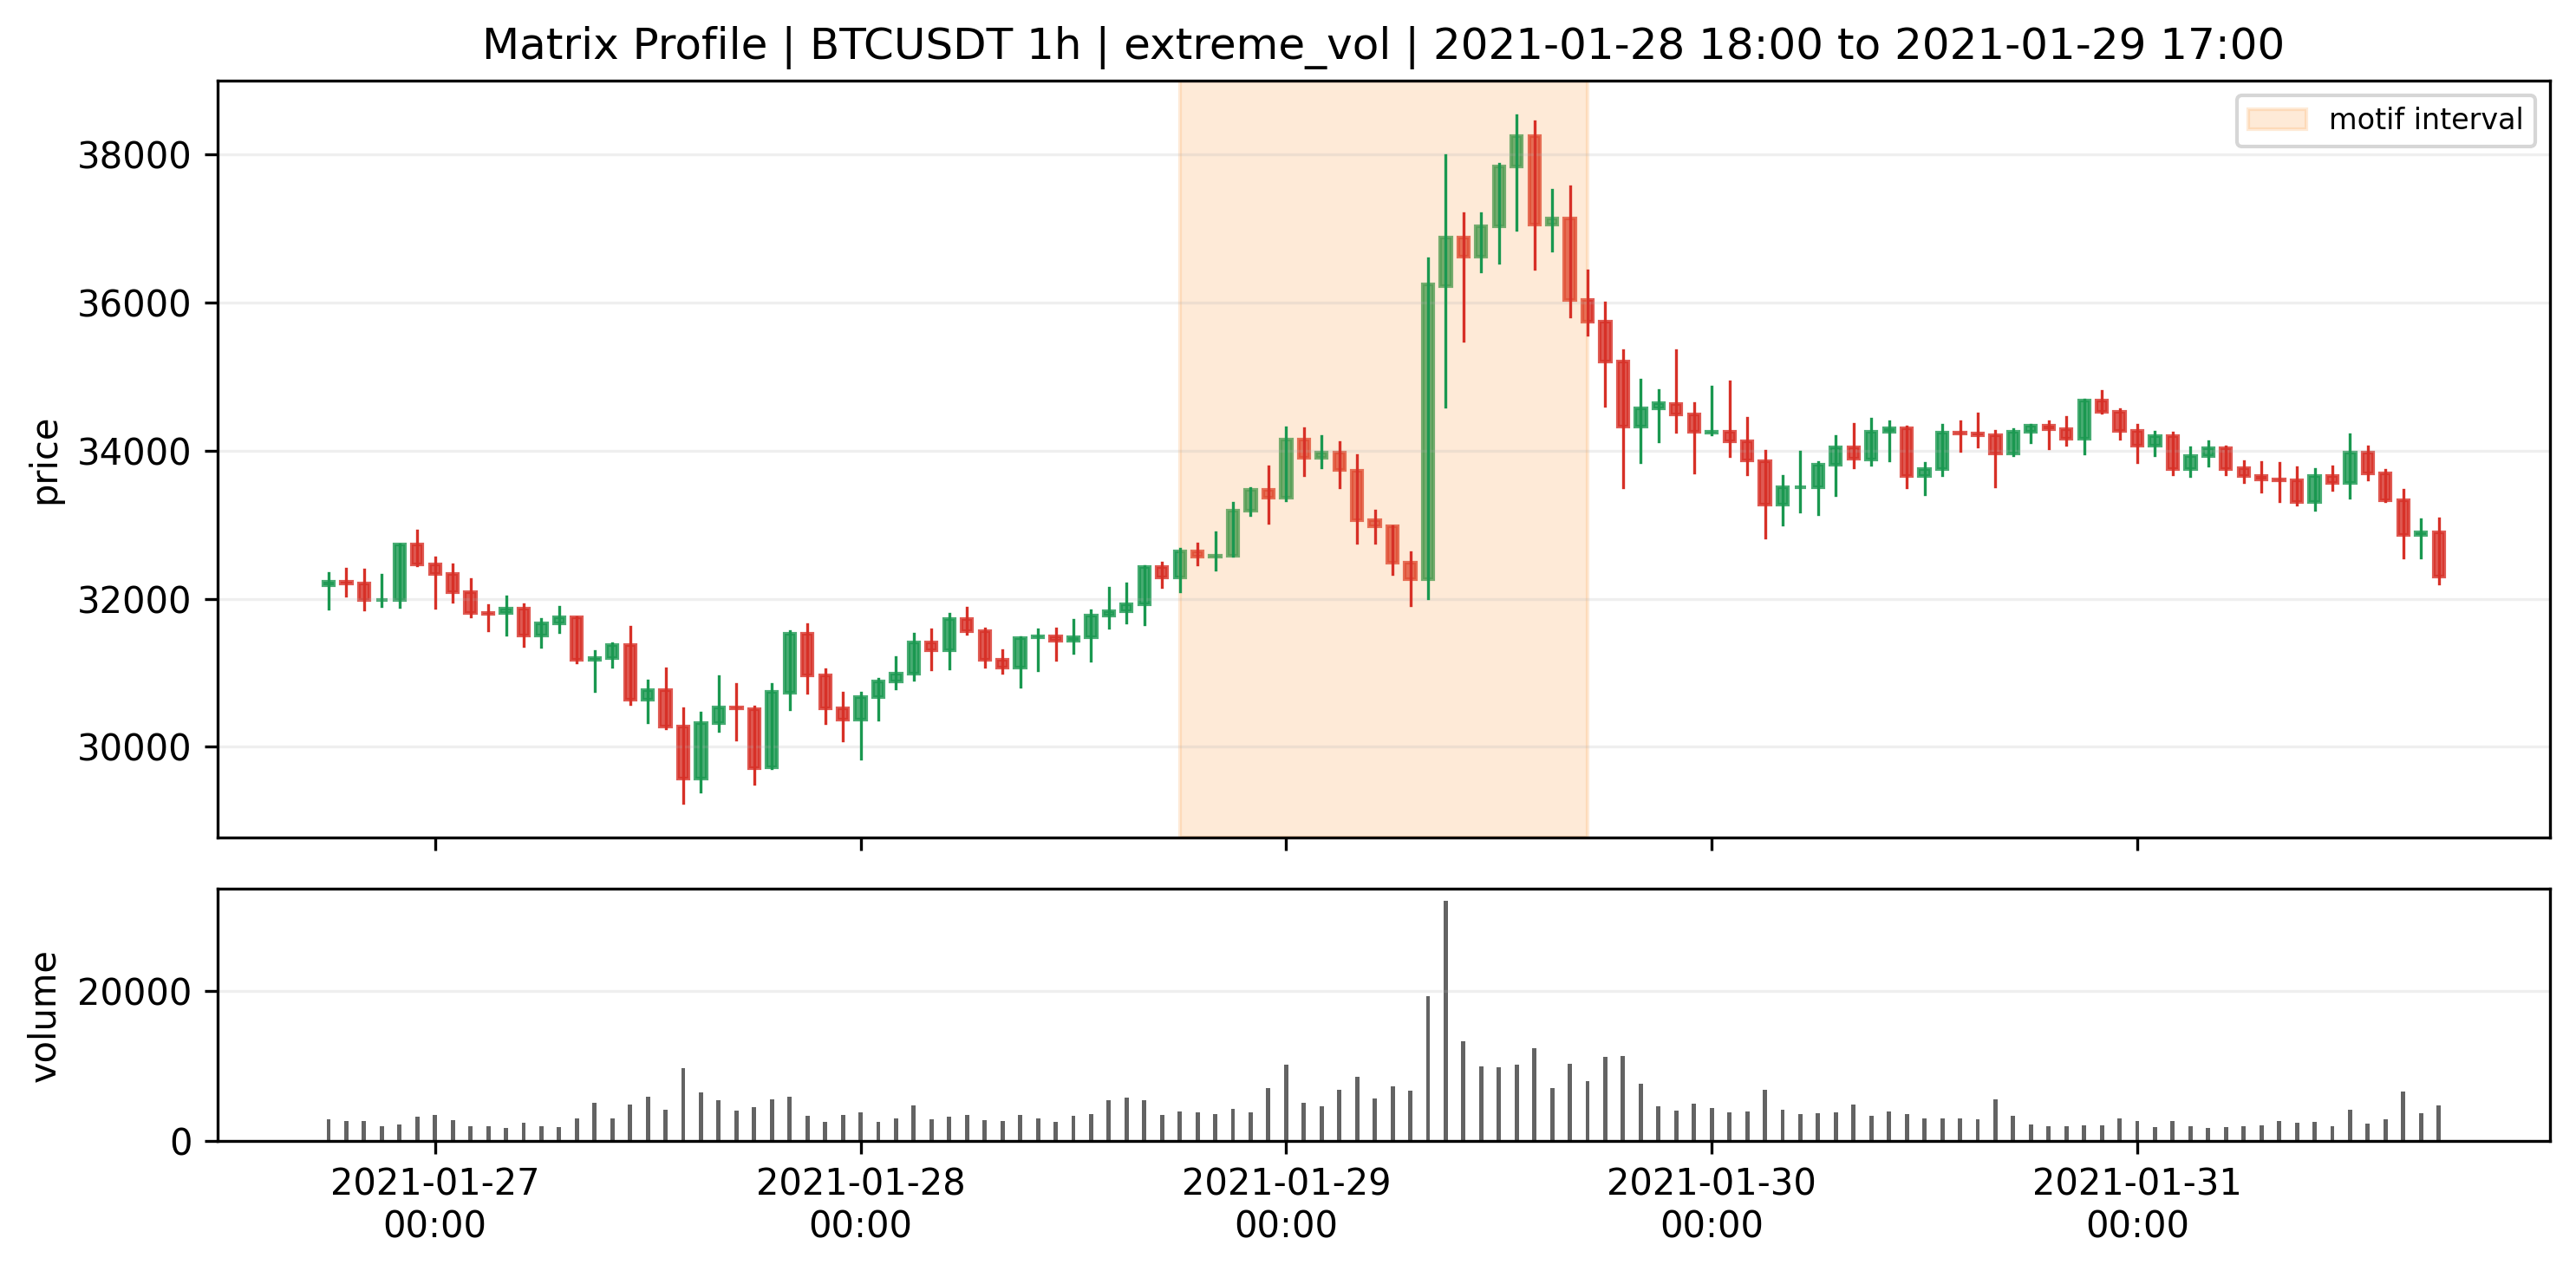
\includegraphics[width=0.9\linewidth]{reports/final_visual_evidence/figures/motif_21_matrix_profile_btcusdt_1h_extreme_vol_1_0_pair59_1_context.png}
\caption{motif 21 matrix profile btcusdt 1h extreme vol 1 0 pair59 1 context. The shaded interval marks the discovered motif occurrence in original price context.}
\end{figure}

\begin{figure}[ht]
\centering
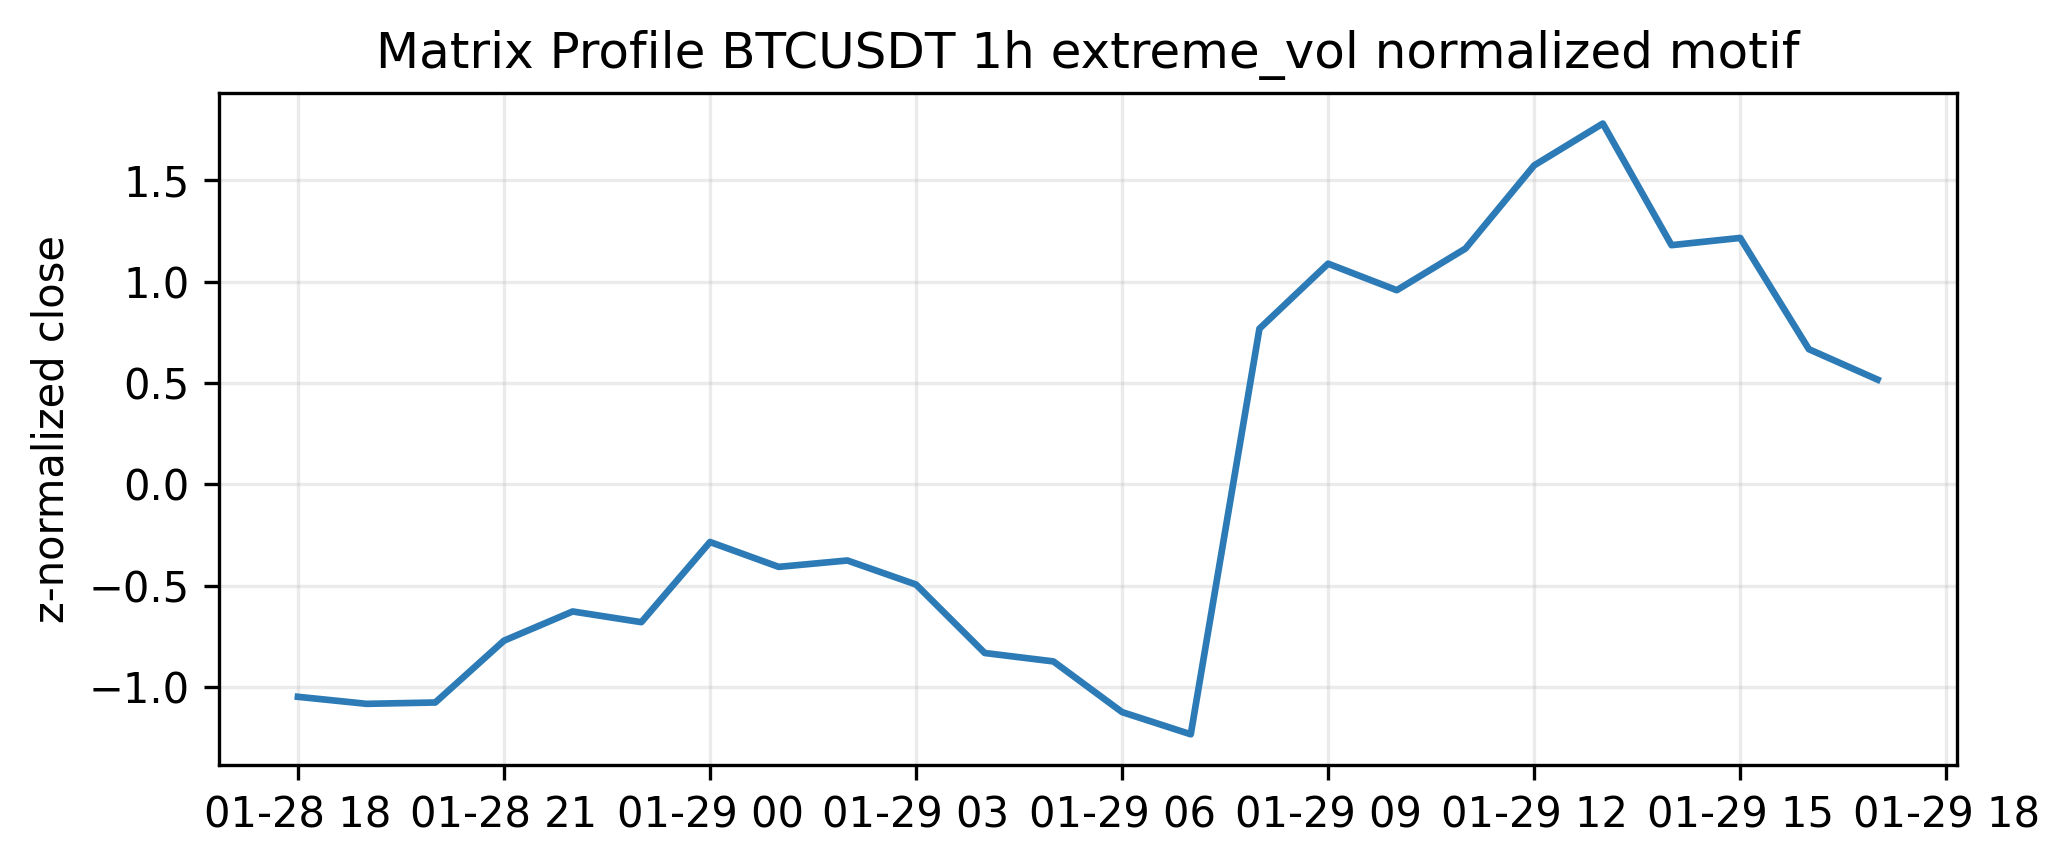
\includegraphics[width=0.9\linewidth]{reports/final_visual_evidence/figures/motif_21_matrix_profile_btcusdt_1h_extreme_vol_1_0_pair59_1_normal_pattern.png}
\caption{motif 21 matrix profile btcusdt 1h extreme vol 1 0 pair59 1 normal pattern. The shaded interval marks the discovered motif occurrence in original price context.}
\end{figure}

\begin{figure}[ht]
\centering
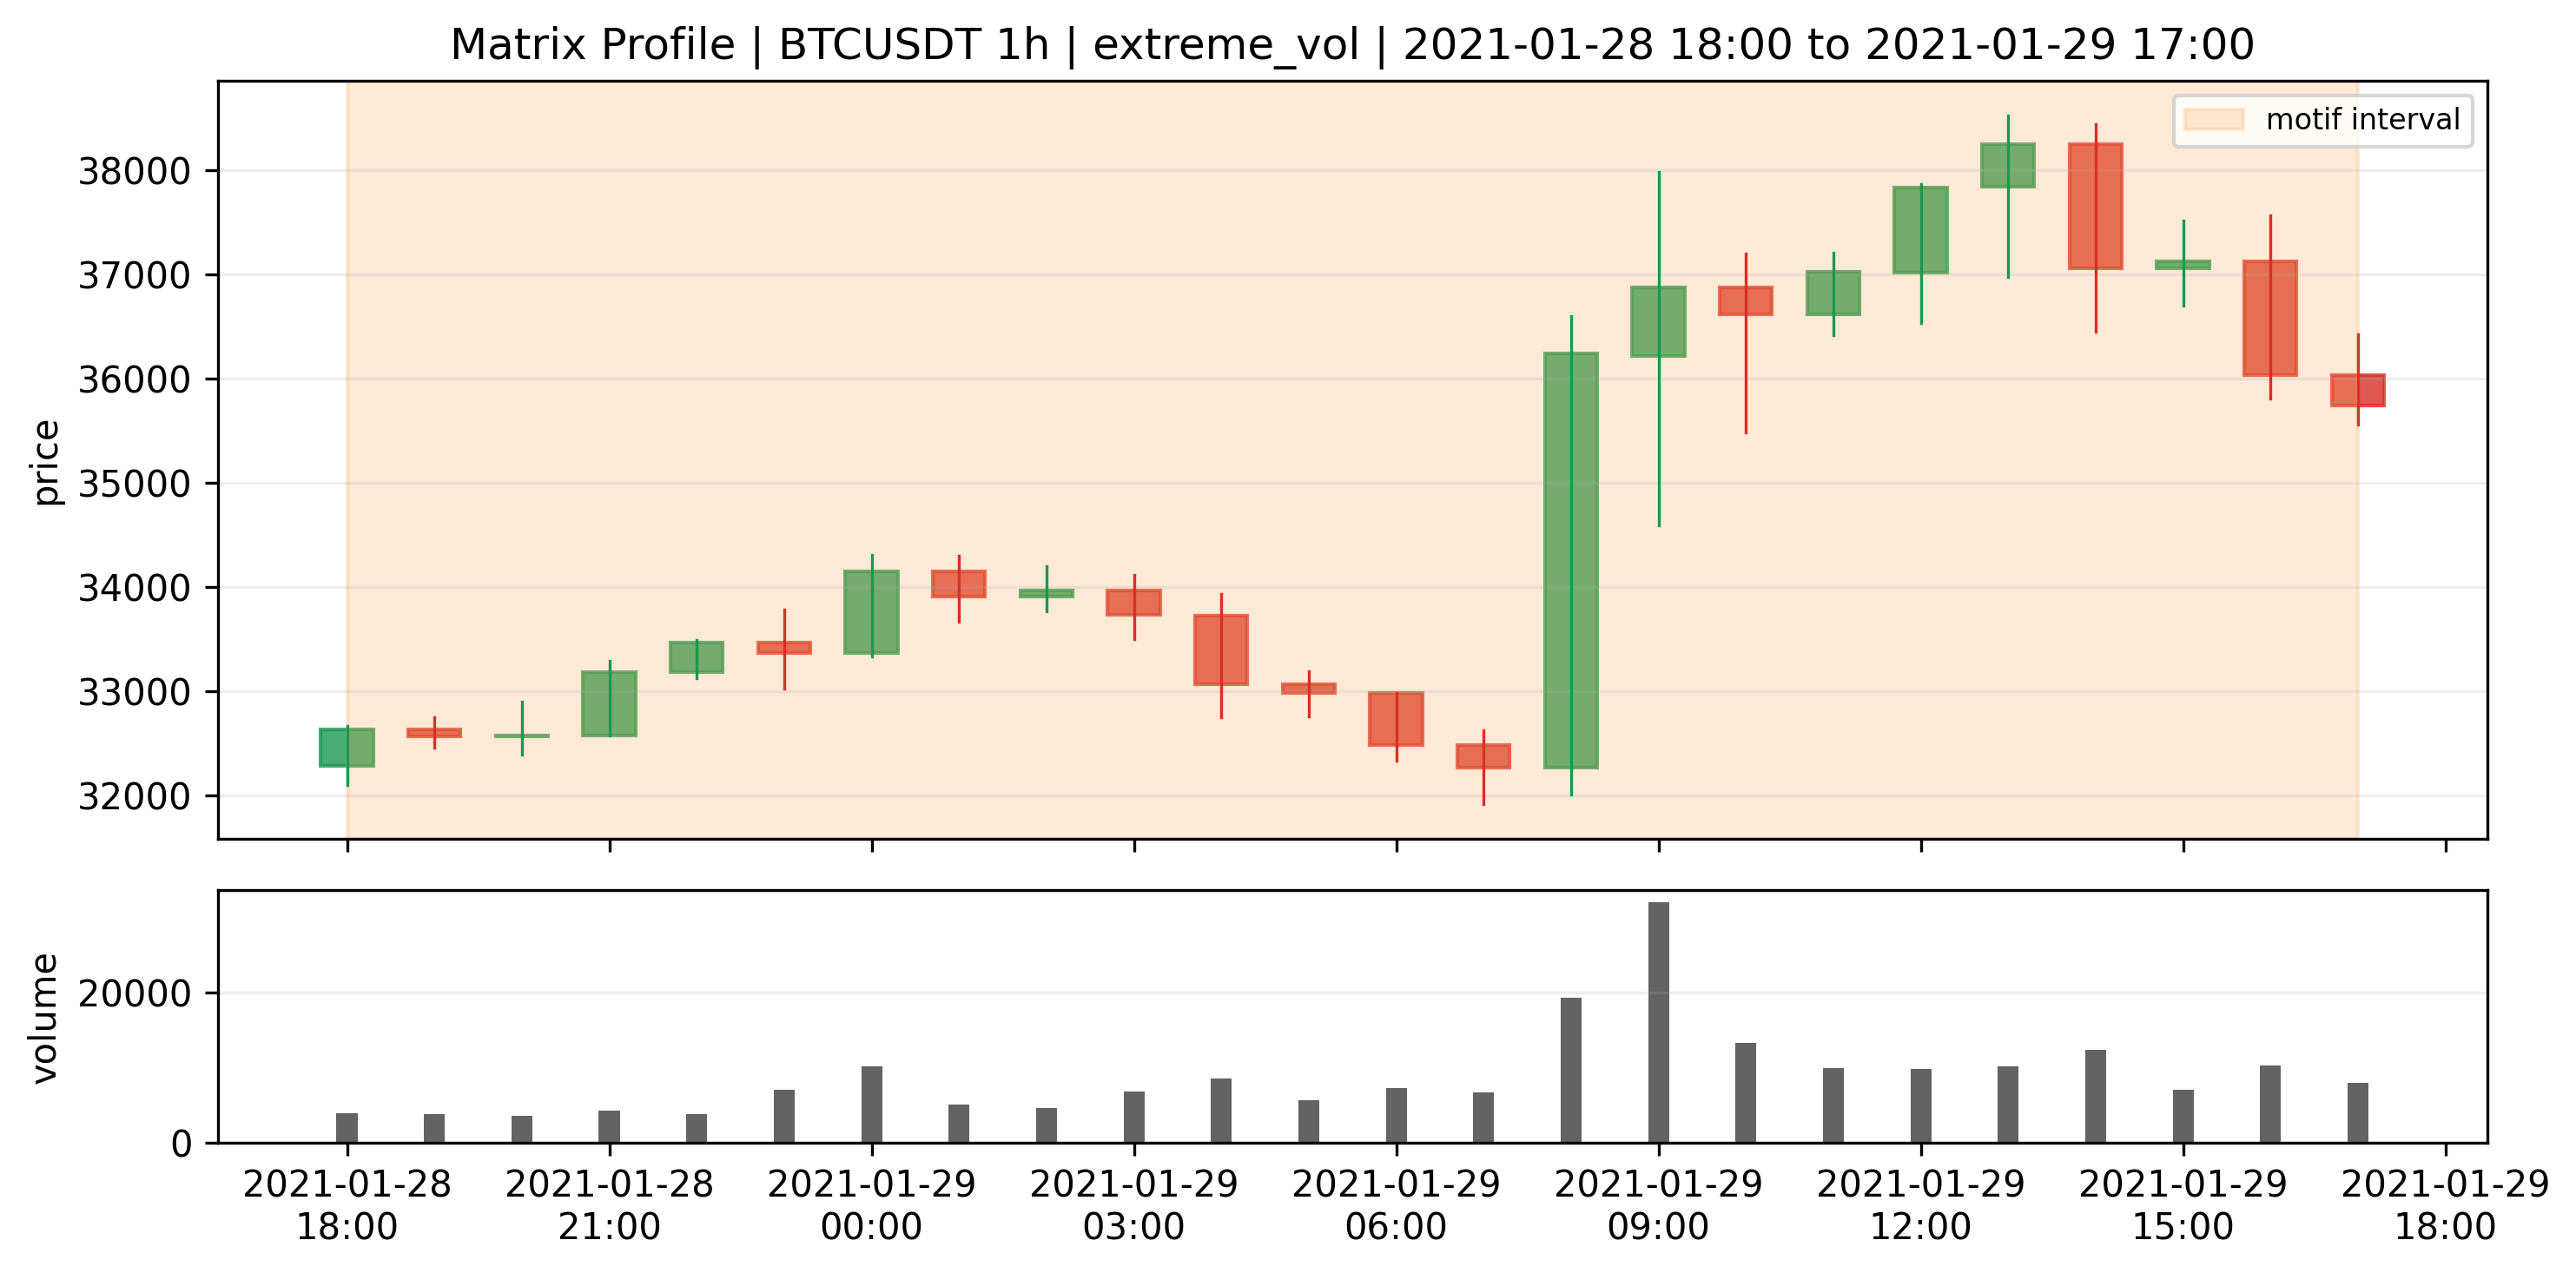
\includegraphics[width=0.9\linewidth]{reports/final_visual_evidence/figures/motif_21_matrix_profile_btcusdt_1h_extreme_vol_1_0_pair59_1_zoom.png}
\caption{motif 21 matrix profile btcusdt 1h extreme vol 1 0 pair59 1 zoom. The shaded interval marks the discovered motif occurrence in original price context.}
\end{figure}

\begin{figure}[ht]
\centering
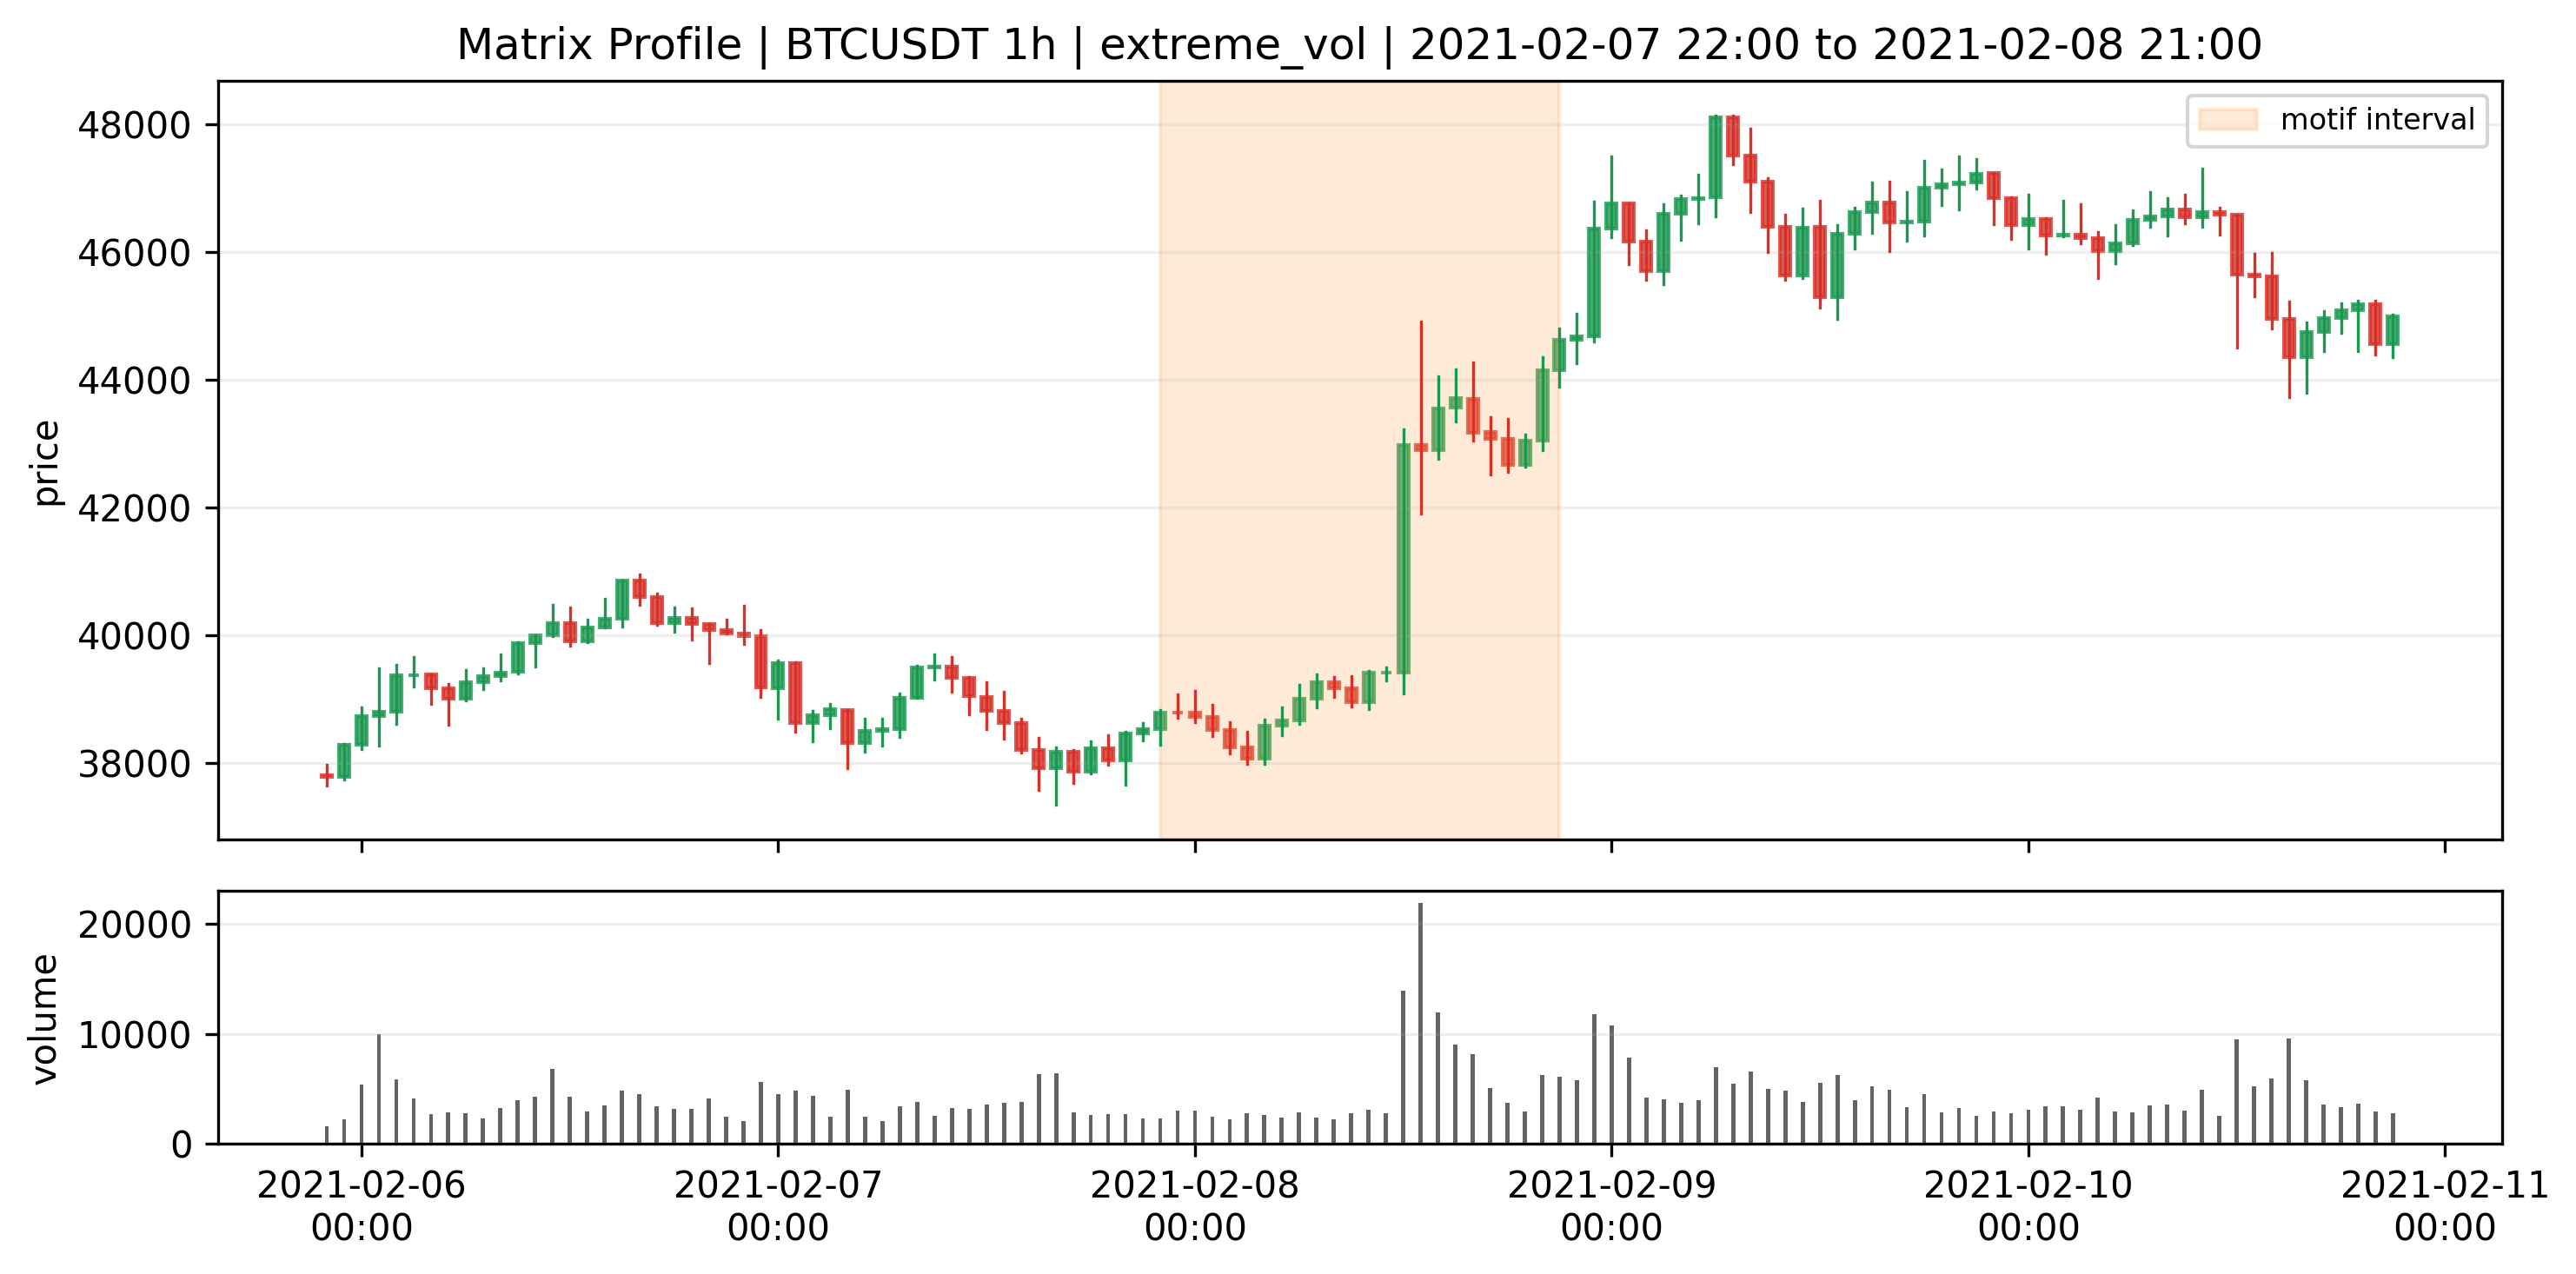
\includegraphics[width=0.9\linewidth]{reports/final_visual_evidence/figures/motif_22_matrix_profile_btcusdt_1h_extreme_vol_1_0_pair59_2_context.png}
\caption{motif 22 matrix profile btcusdt 1h extreme vol 1 0 pair59 2 context. The shaded interval marks the discovered motif occurrence in original price context.}
\end{figure}

\begin{figure}[ht]
\centering
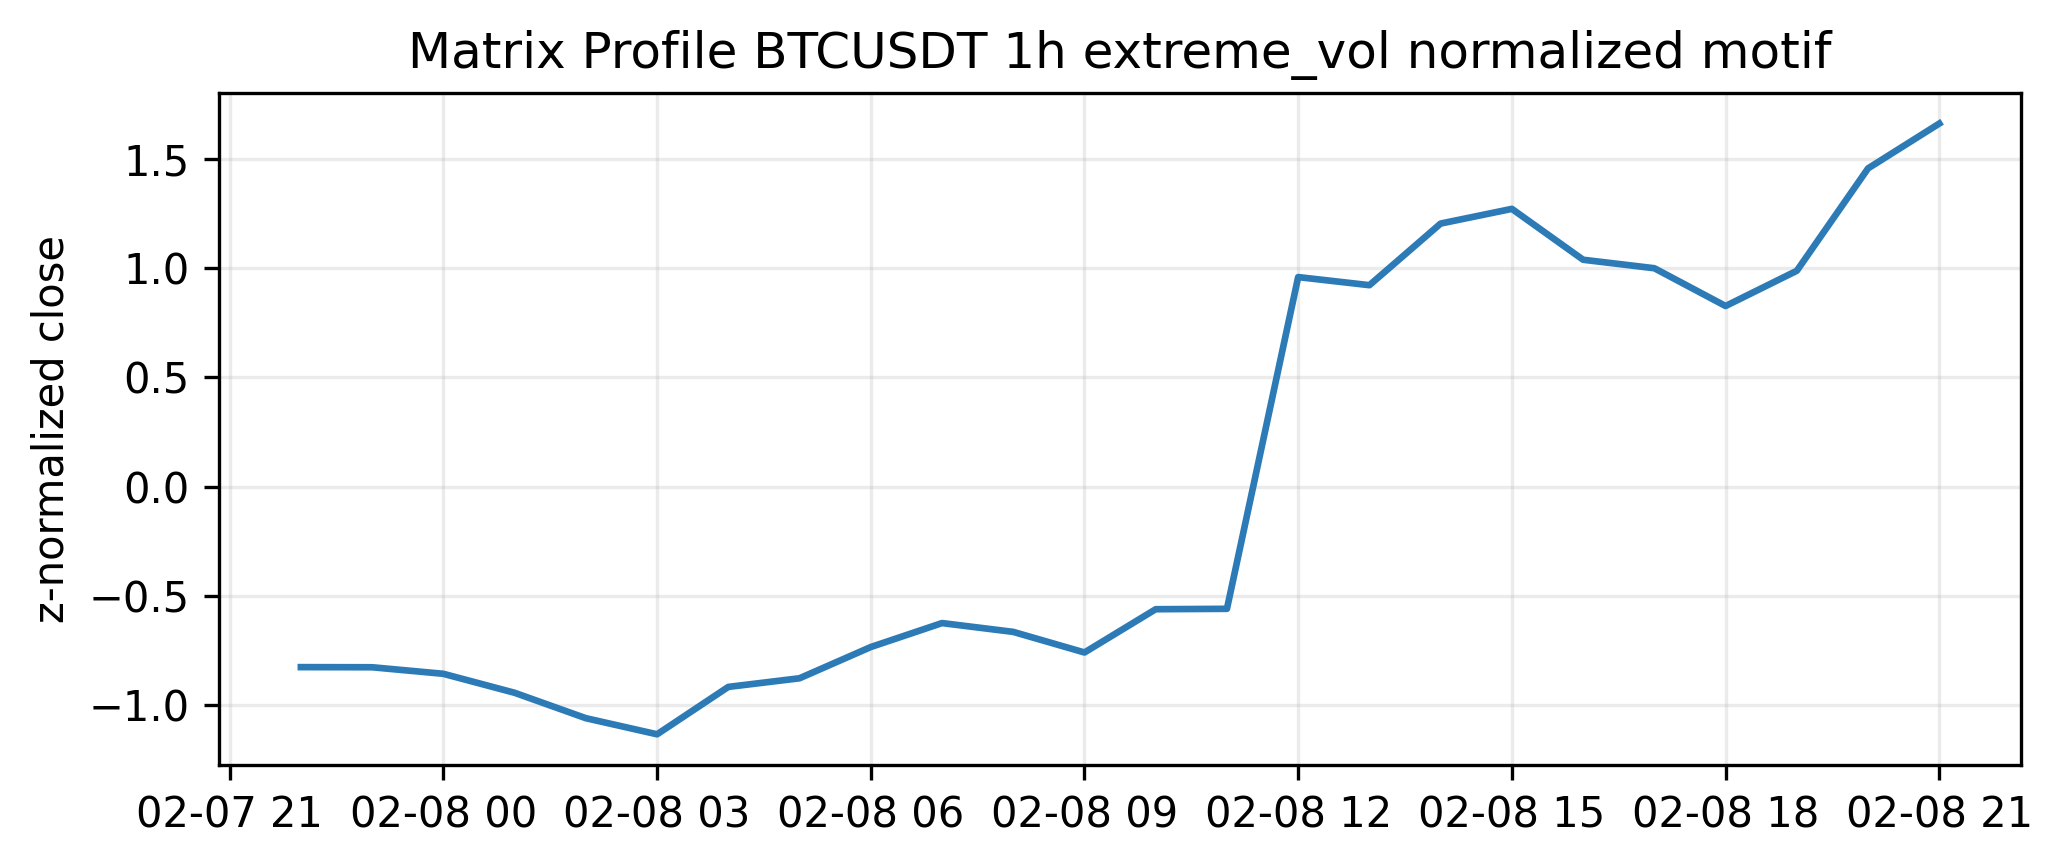
\includegraphics[width=0.9\linewidth]{reports/final_visual_evidence/figures/motif_22_matrix_profile_btcusdt_1h_extreme_vol_1_0_pair59_2_normal_pattern.png}
\caption{motif 22 matrix profile btcusdt 1h extreme vol 1 0 pair59 2 normal pattern. The shaded interval marks the discovered motif occurrence in original price context.}
\end{figure}

\begin{figure}[ht]
\centering
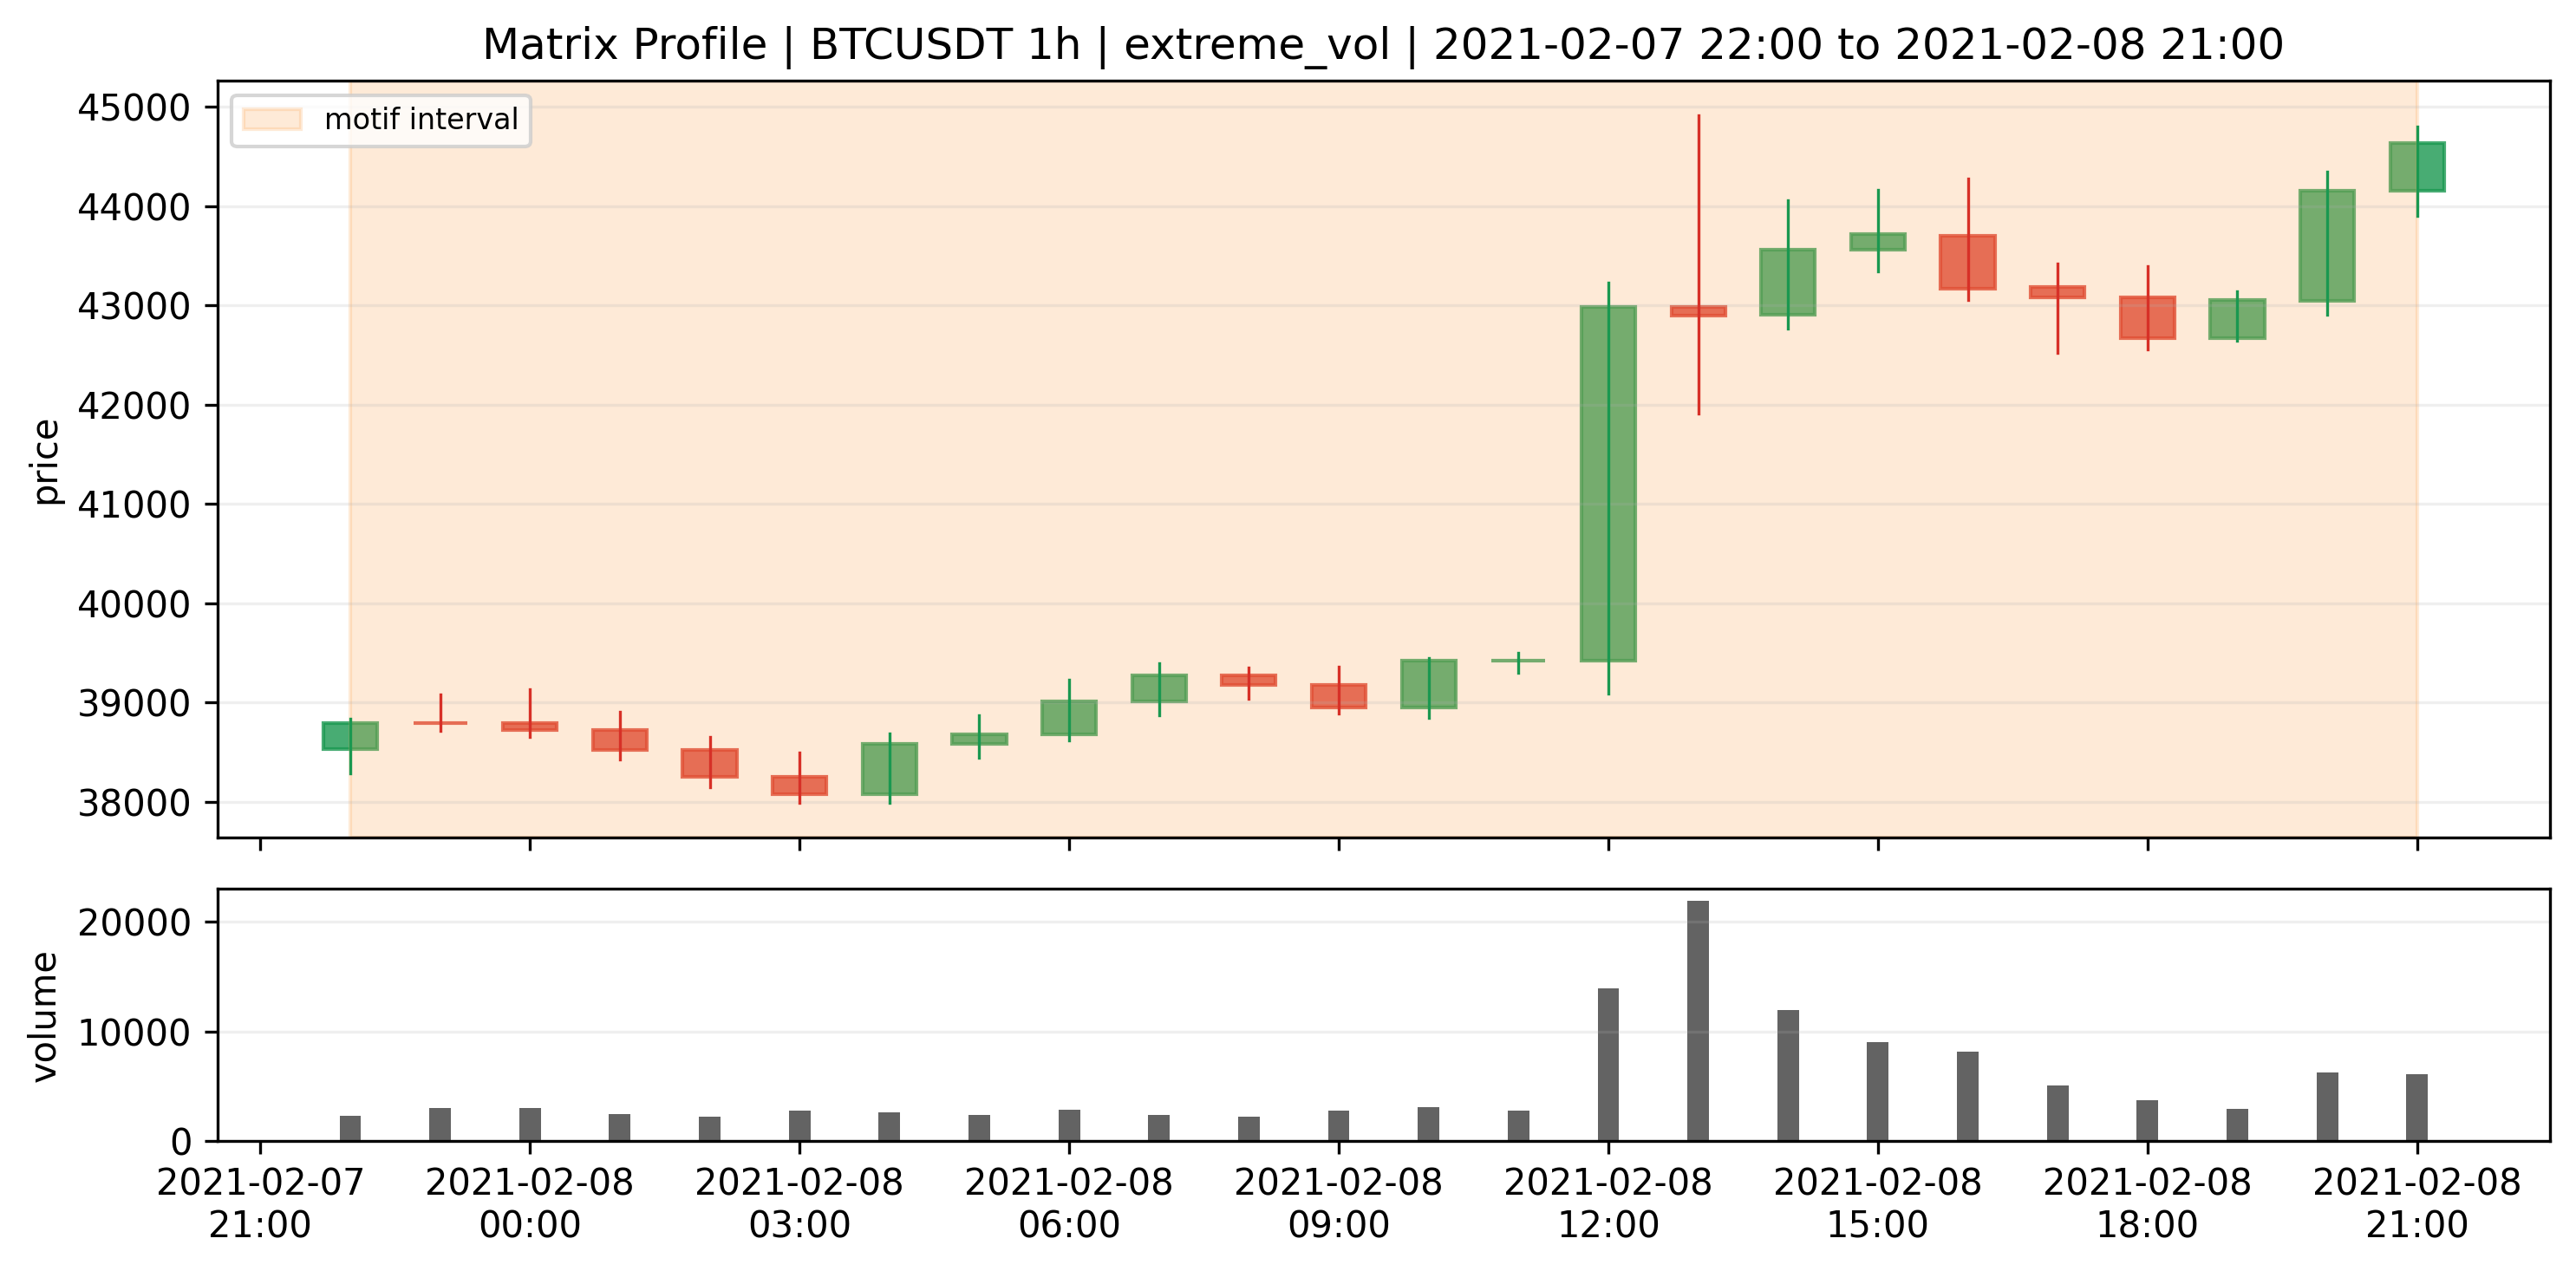
\includegraphics[width=0.9\linewidth]{reports/final_visual_evidence/figures/motif_22_matrix_profile_btcusdt_1h_extreme_vol_1_0_pair59_2_zoom.png}
\caption{motif 22 matrix profile btcusdt 1h extreme vol 1 0 pair59 2 zoom. The shaded interval marks the discovered motif occurrence in original price context.}
\end{figure}

\begin{figure}[ht]
\centering
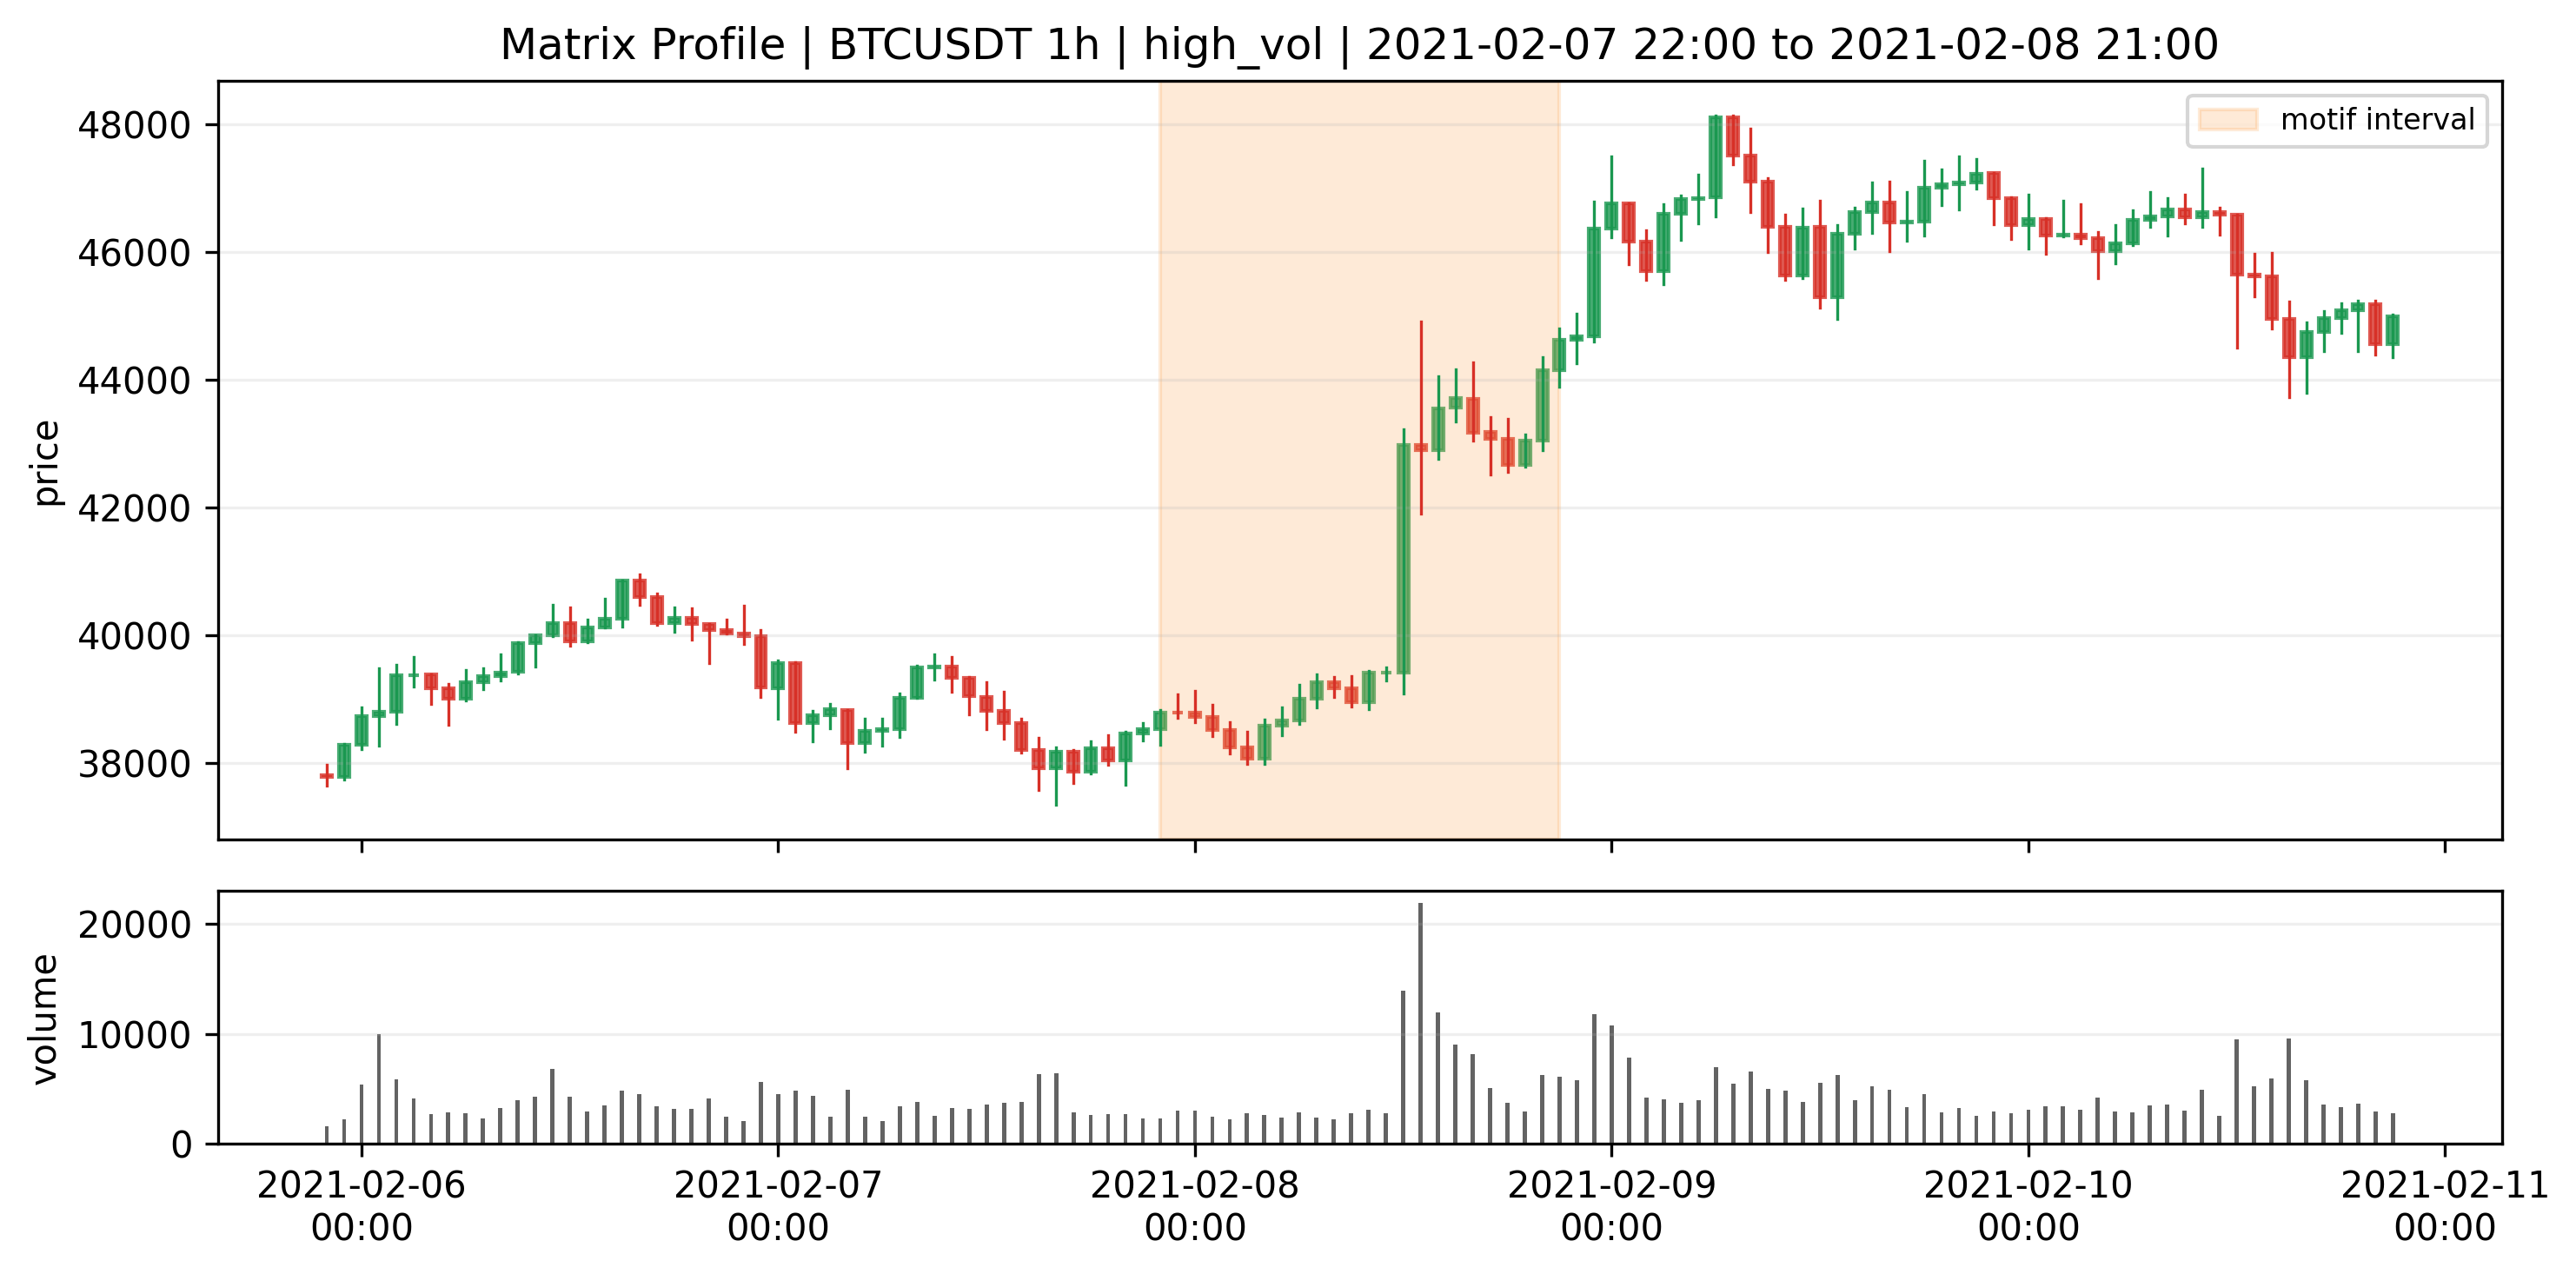
\includegraphics[width=0.9\linewidth]{reports/final_visual_evidence/figures/motif_23_matrix_profile_btcusdt_1h_high_vol_1_0_pair45_1_context.png}
\caption{motif 23 matrix profile btcusdt 1h high vol 1 0 pair45 1 context. The shaded interval marks the discovered motif occurrence in original price context.}
\end{figure}

\begin{figure}[ht]
\centering
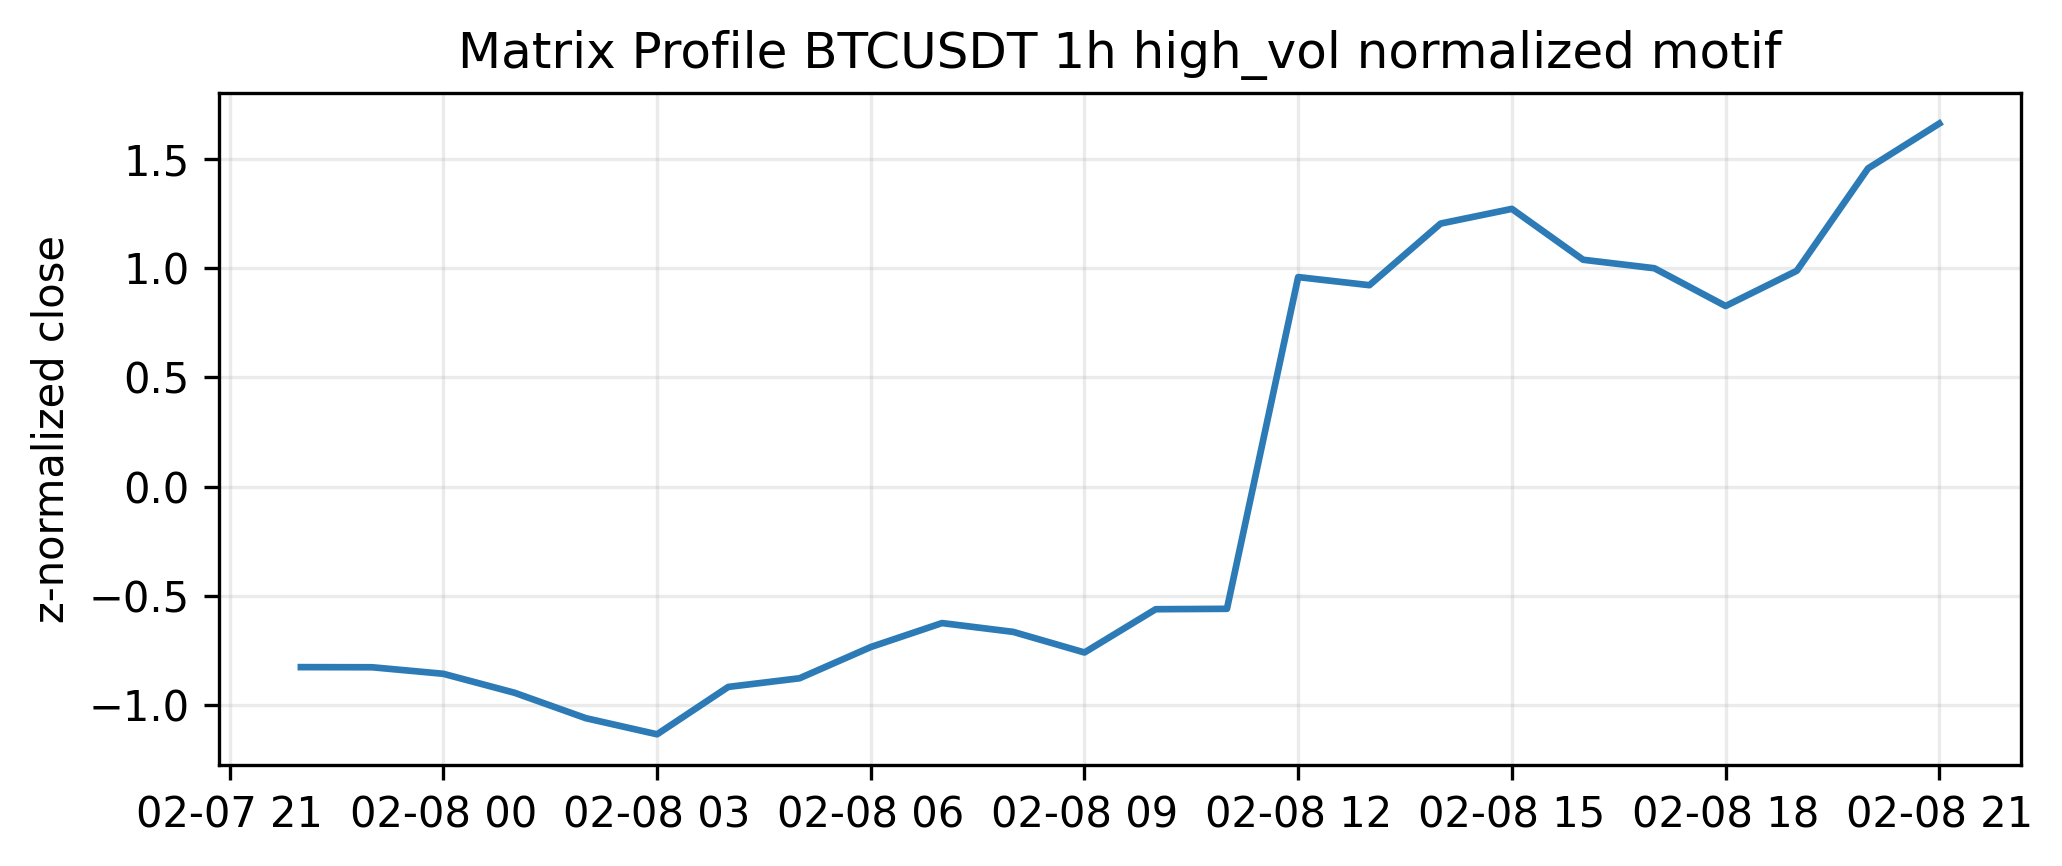
\includegraphics[width=0.9\linewidth]{reports/final_visual_evidence/figures/motif_23_matrix_profile_btcusdt_1h_high_vol_1_0_pair45_1_normal_pattern.png}
\caption{motif 23 matrix profile btcusdt 1h high vol 1 0 pair45 1 normal pattern. The shaded interval marks the discovered motif occurrence in original price context.}
\end{figure}

\begin{figure}[ht]
\centering
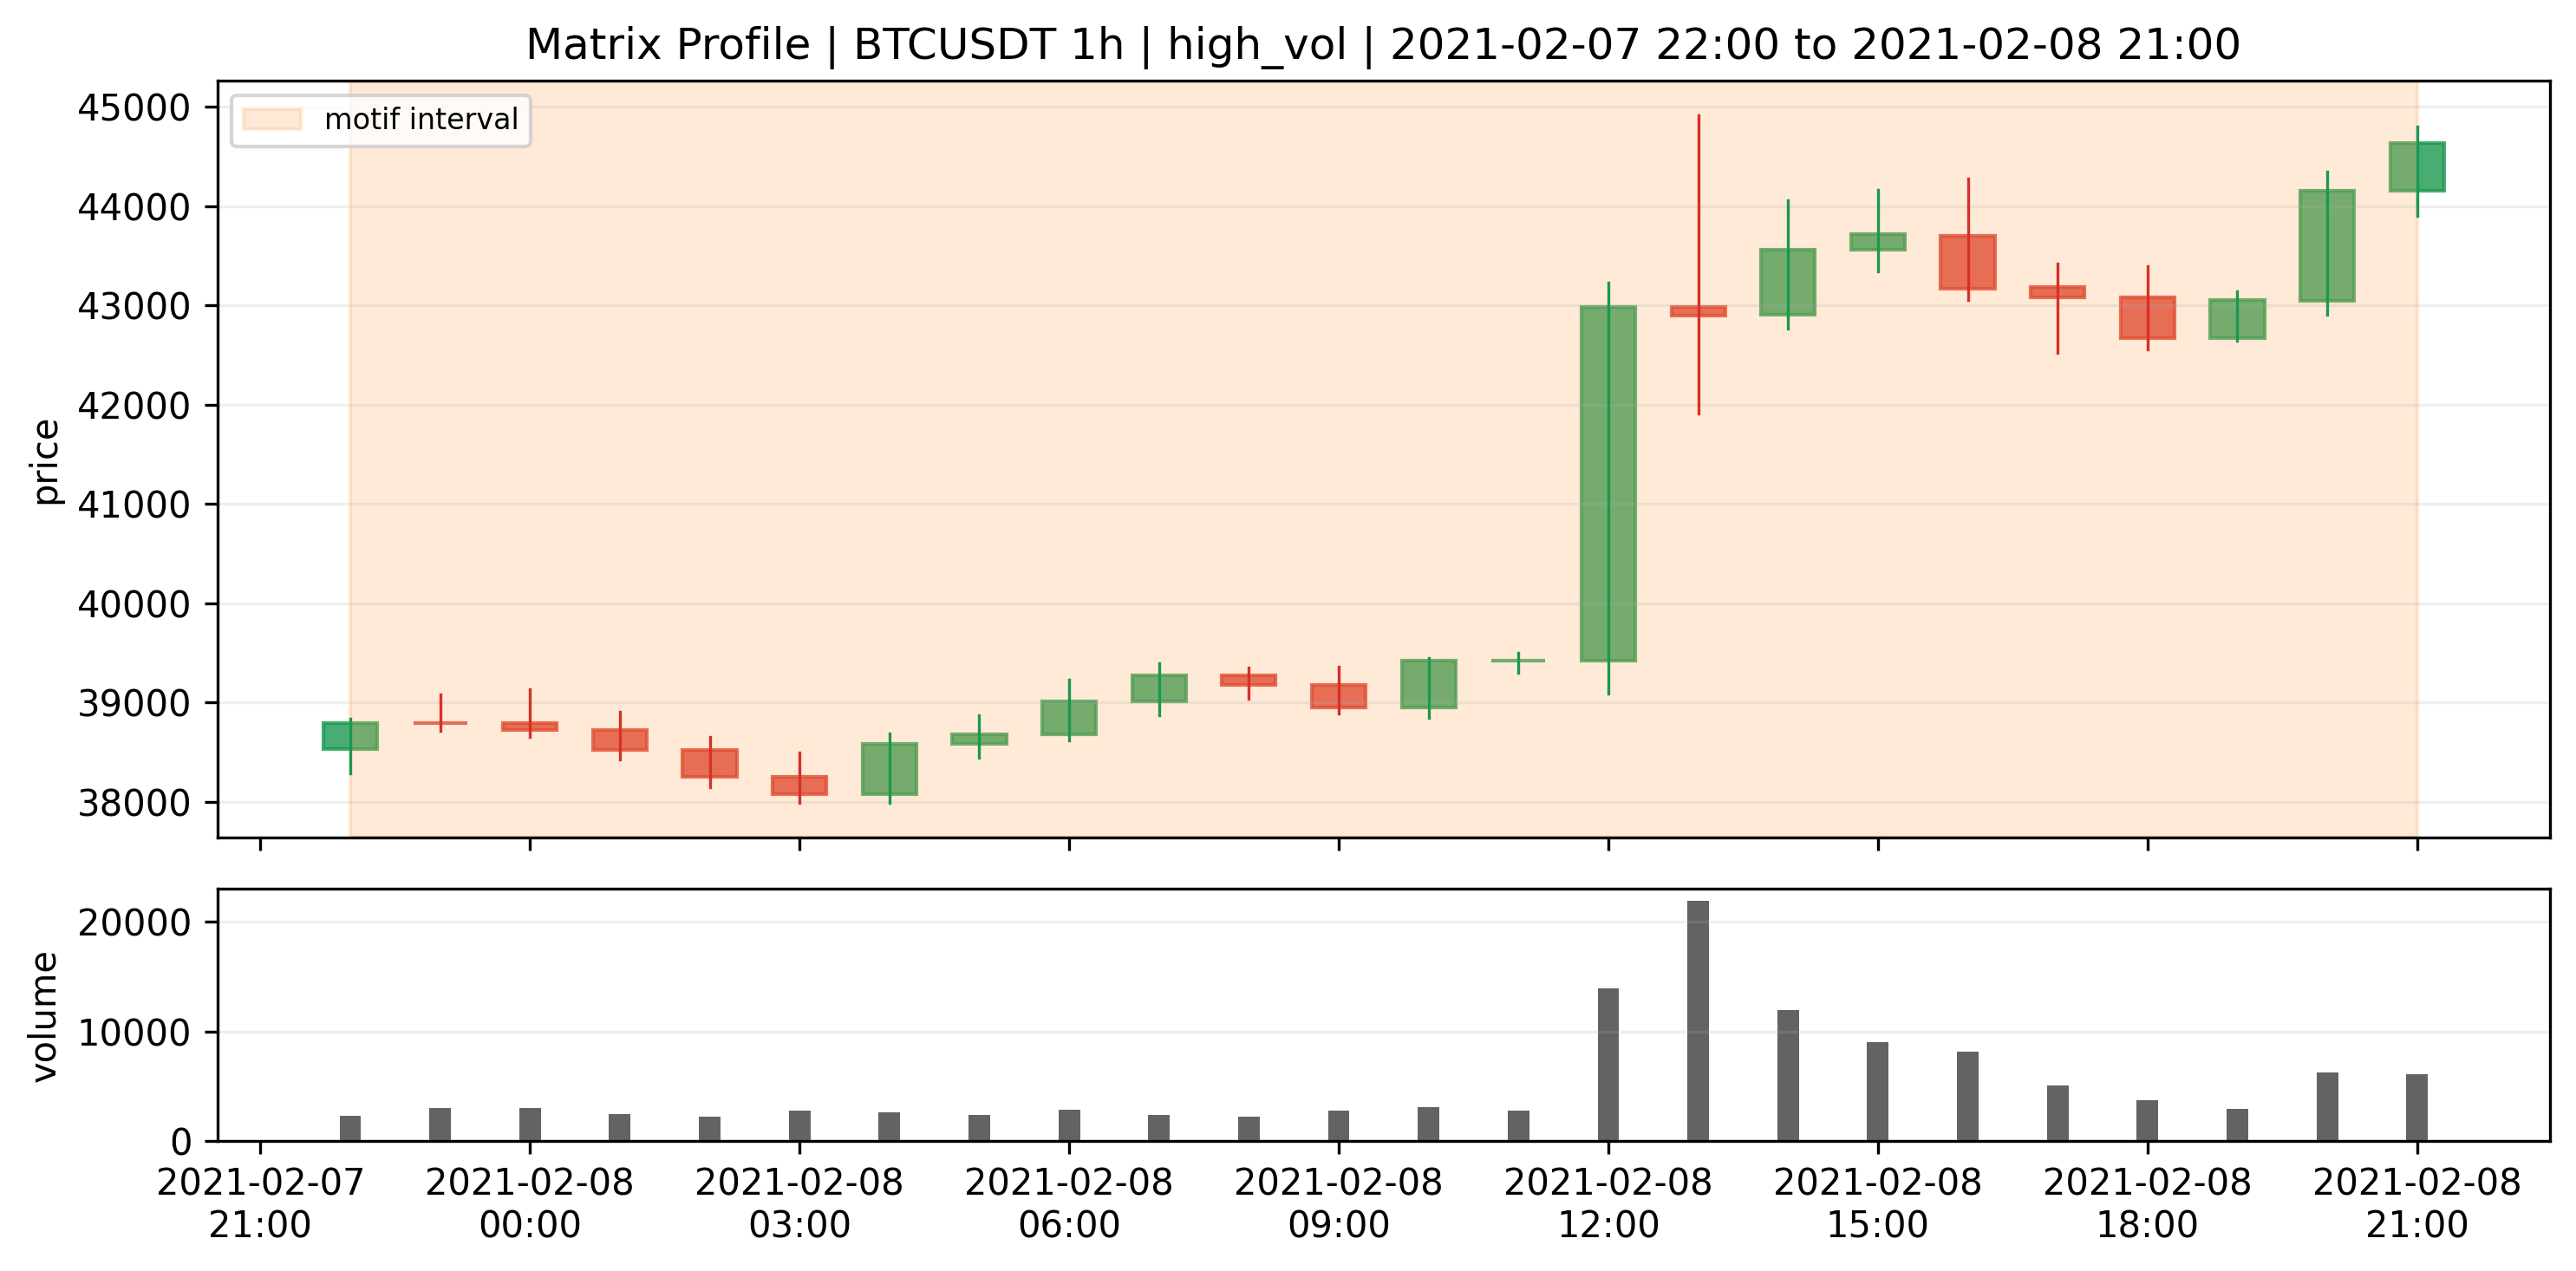
\includegraphics[width=0.9\linewidth]{reports/final_visual_evidence/figures/motif_23_matrix_profile_btcusdt_1h_high_vol_1_0_pair45_1_zoom.png}
\caption{motif 23 matrix profile btcusdt 1h high vol 1 0 pair45 1 zoom. The shaded interval marks the discovered motif occurrence in original price context.}
\end{figure}

\begin{figure}[ht]
\centering
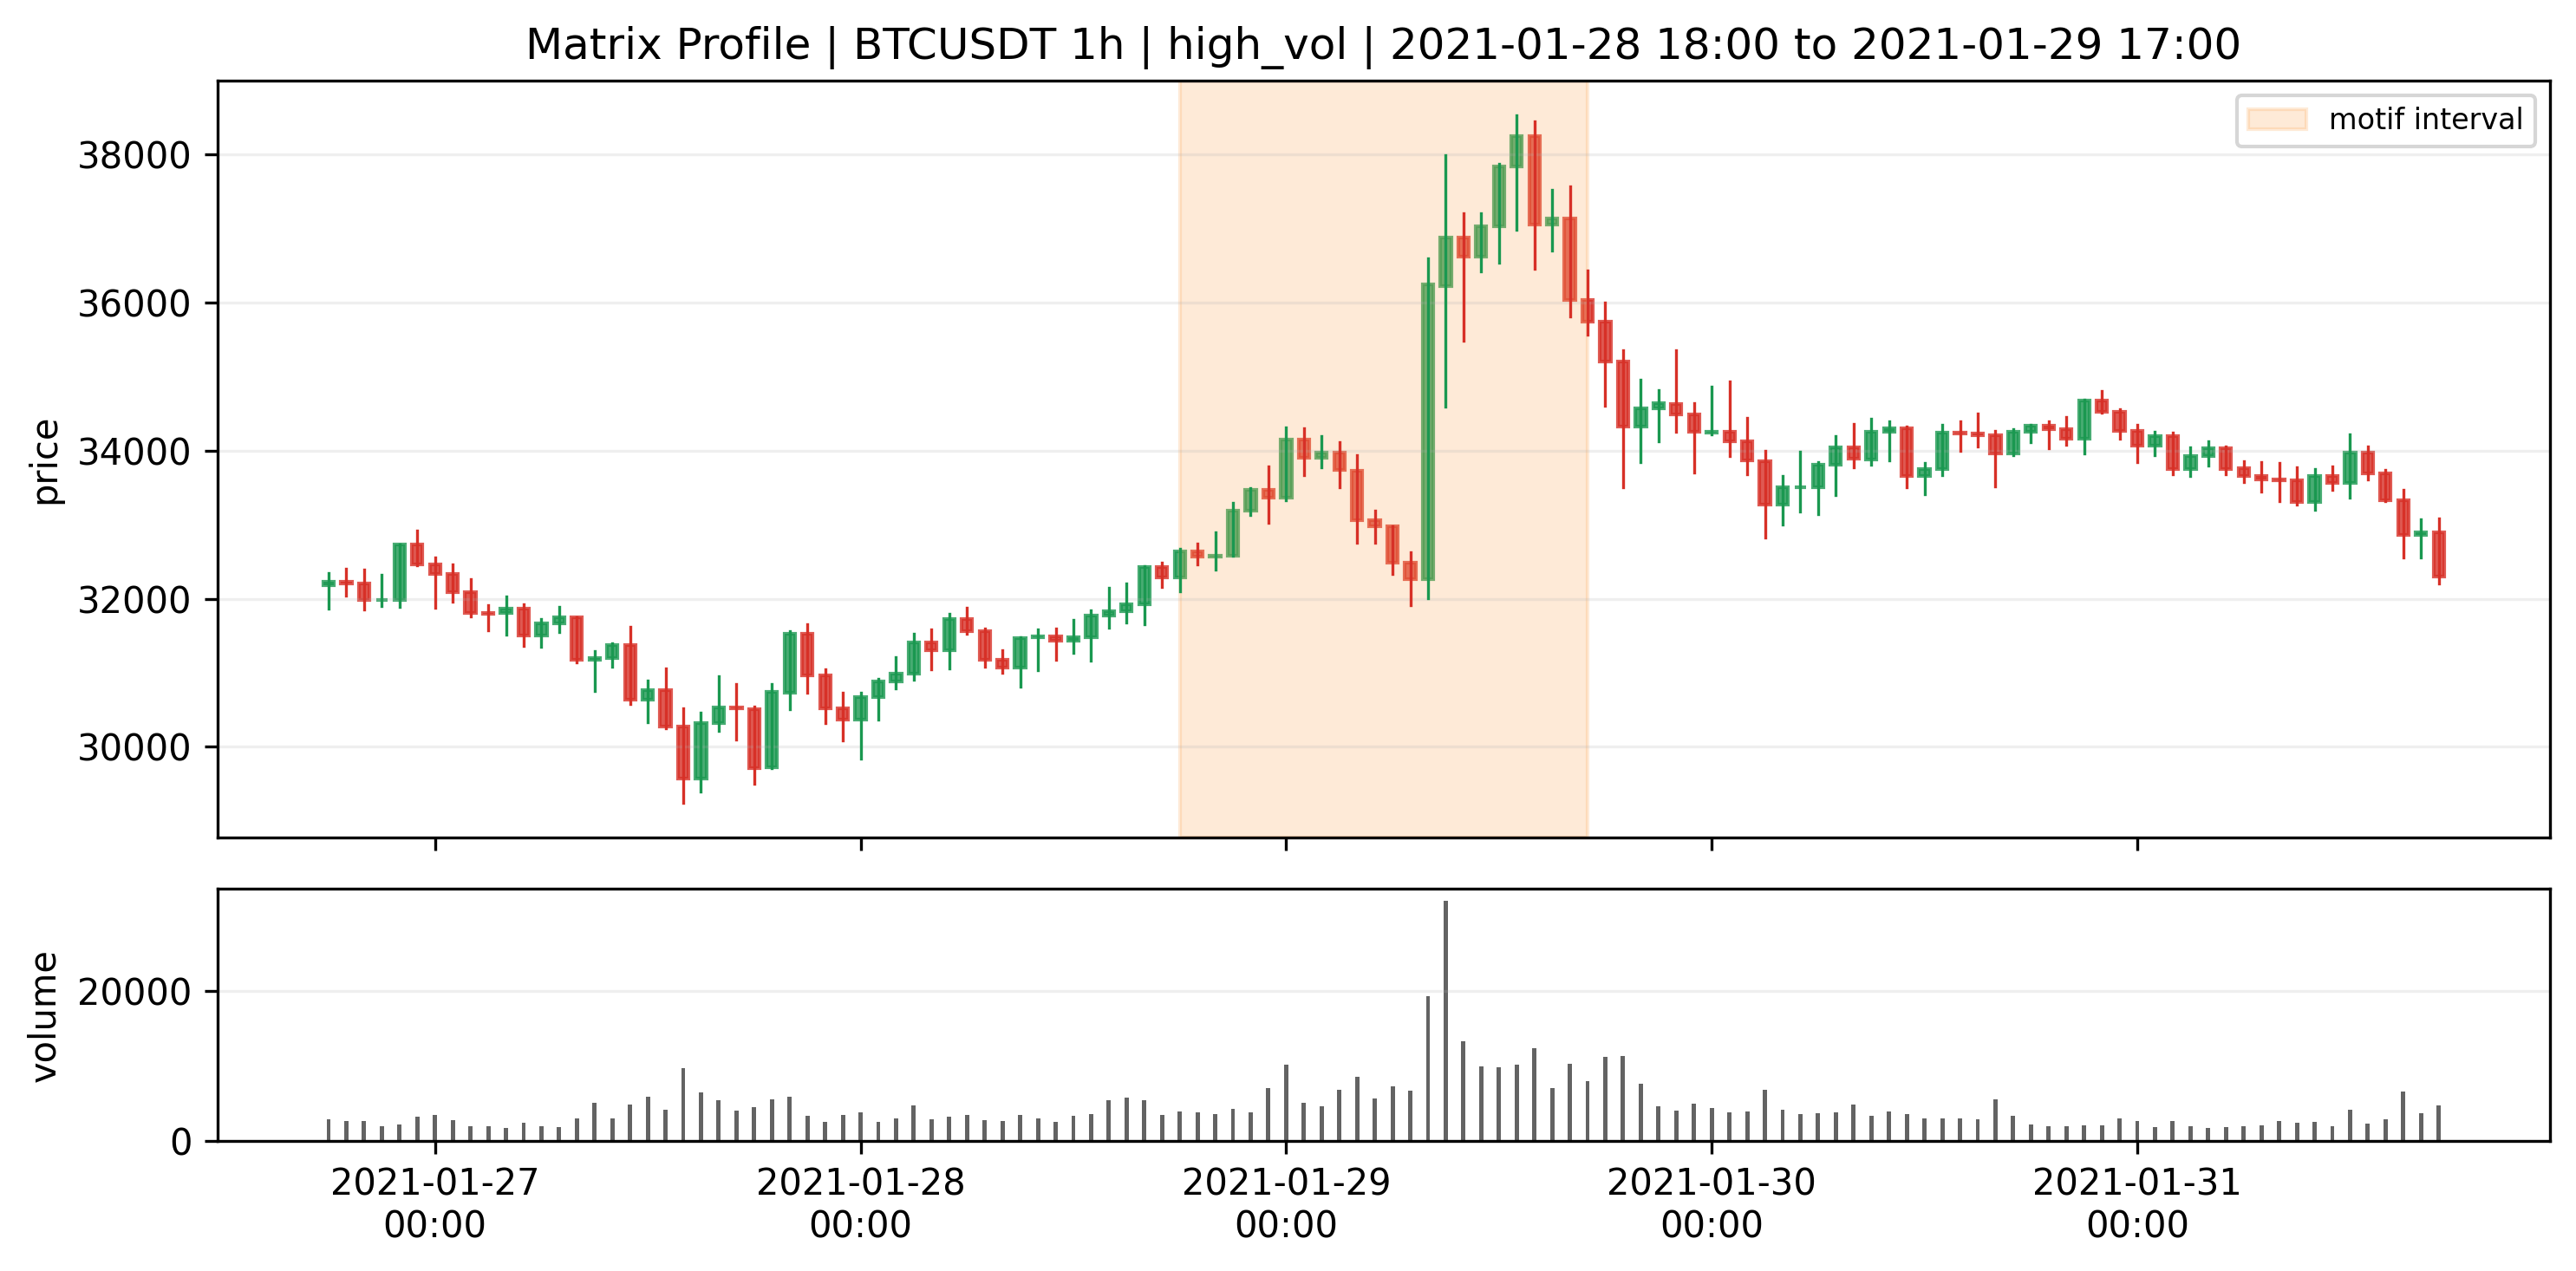
\includegraphics[width=0.9\linewidth]{reports/final_visual_evidence/figures/motif_24_matrix_profile_btcusdt_1h_high_vol_1_0_pair45_2_context.png}
\caption{motif 24 matrix profile btcusdt 1h high vol 1 0 pair45 2 context. The shaded interval marks the discovered motif occurrence in original price context.}
\end{figure}

\begin{figure}[ht]
\centering
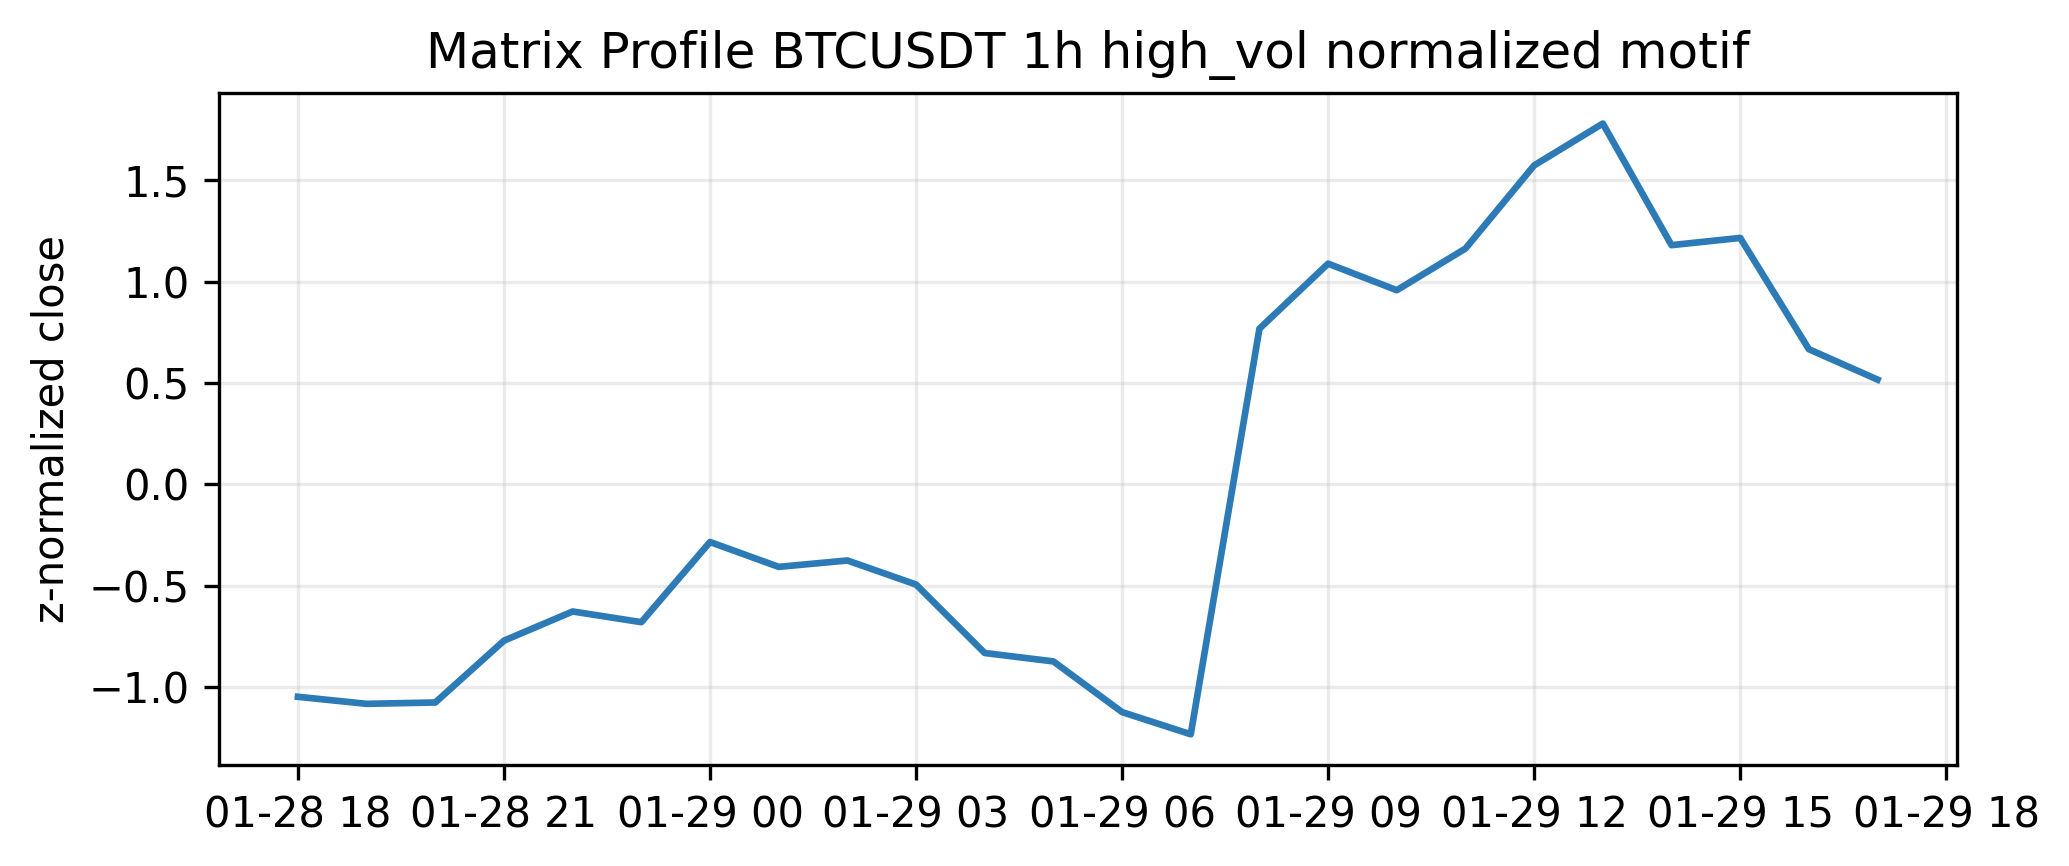
\includegraphics[width=0.9\linewidth]{reports/final_visual_evidence/figures/motif_24_matrix_profile_btcusdt_1h_high_vol_1_0_pair45_2_normal_pattern.png}
\caption{motif 24 matrix profile btcusdt 1h high vol 1 0 pair45 2 normal pattern. The shaded interval marks the discovered motif occurrence in original price context.}
\end{figure}

\begin{figure}[ht]
\centering
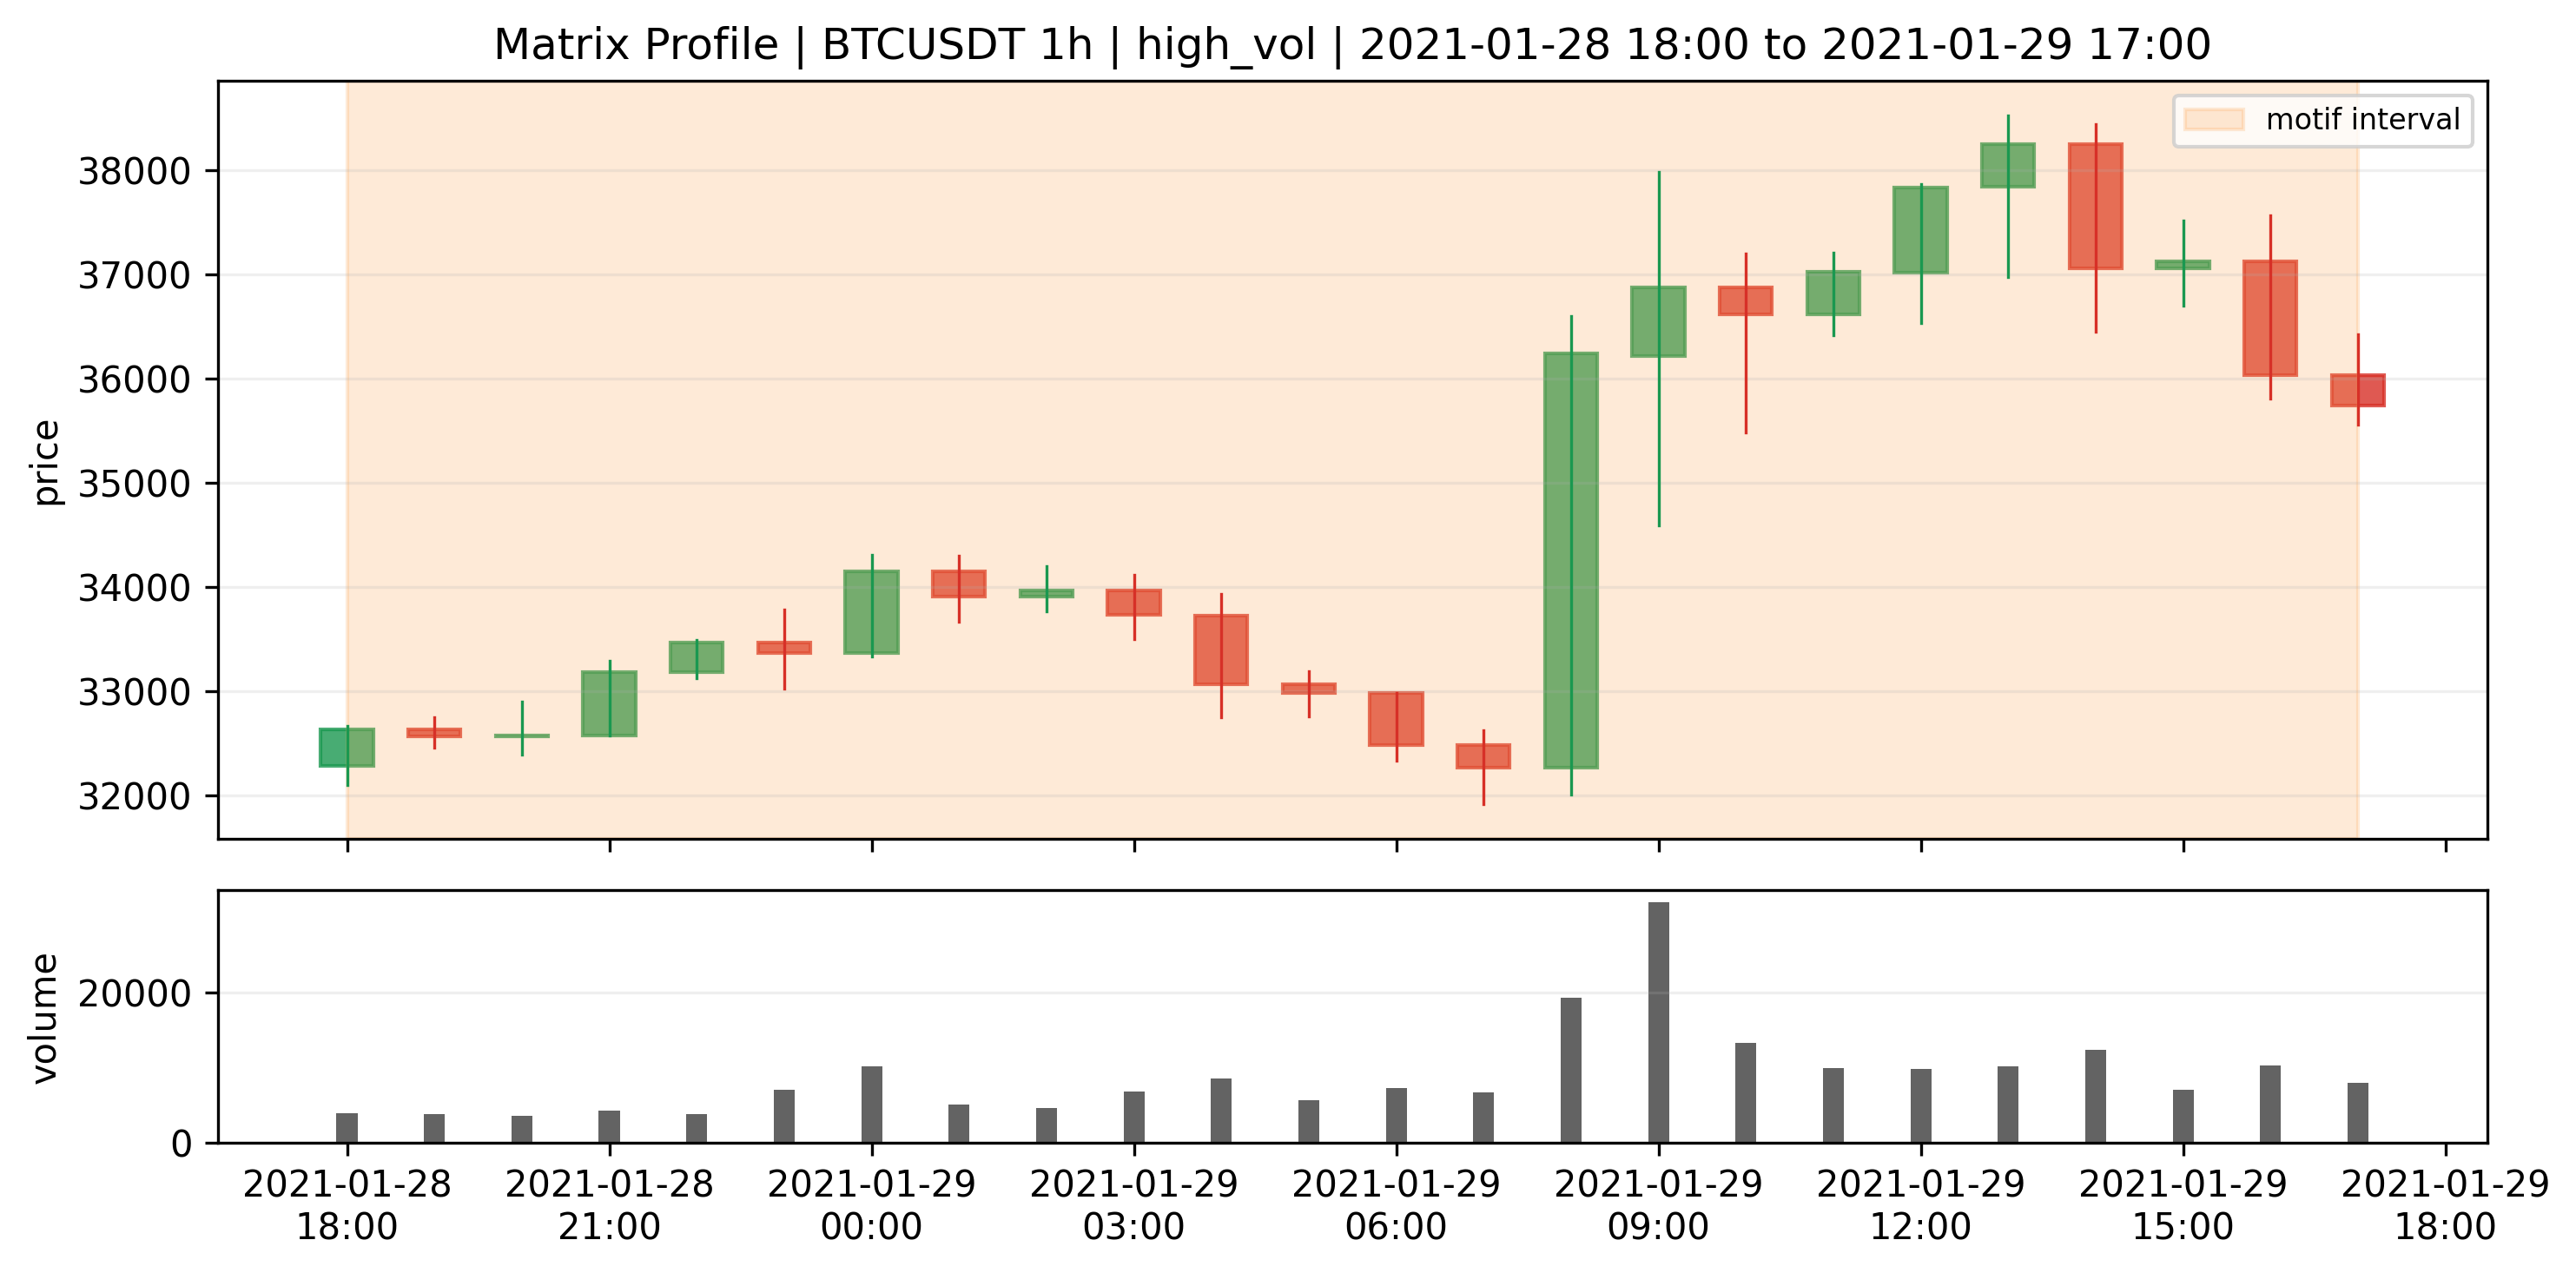
\includegraphics[width=0.9\linewidth]{reports/final_visual_evidence/figures/motif_24_matrix_profile_btcusdt_1h_high_vol_1_0_pair45_2_zoom.png}
\caption{motif 24 matrix profile btcusdt 1h high vol 1 0 pair45 2 zoom. The shaded interval marks the discovered motif occurrence in original price context.}
\end{figure}

\begin{figure}[ht]
\centering
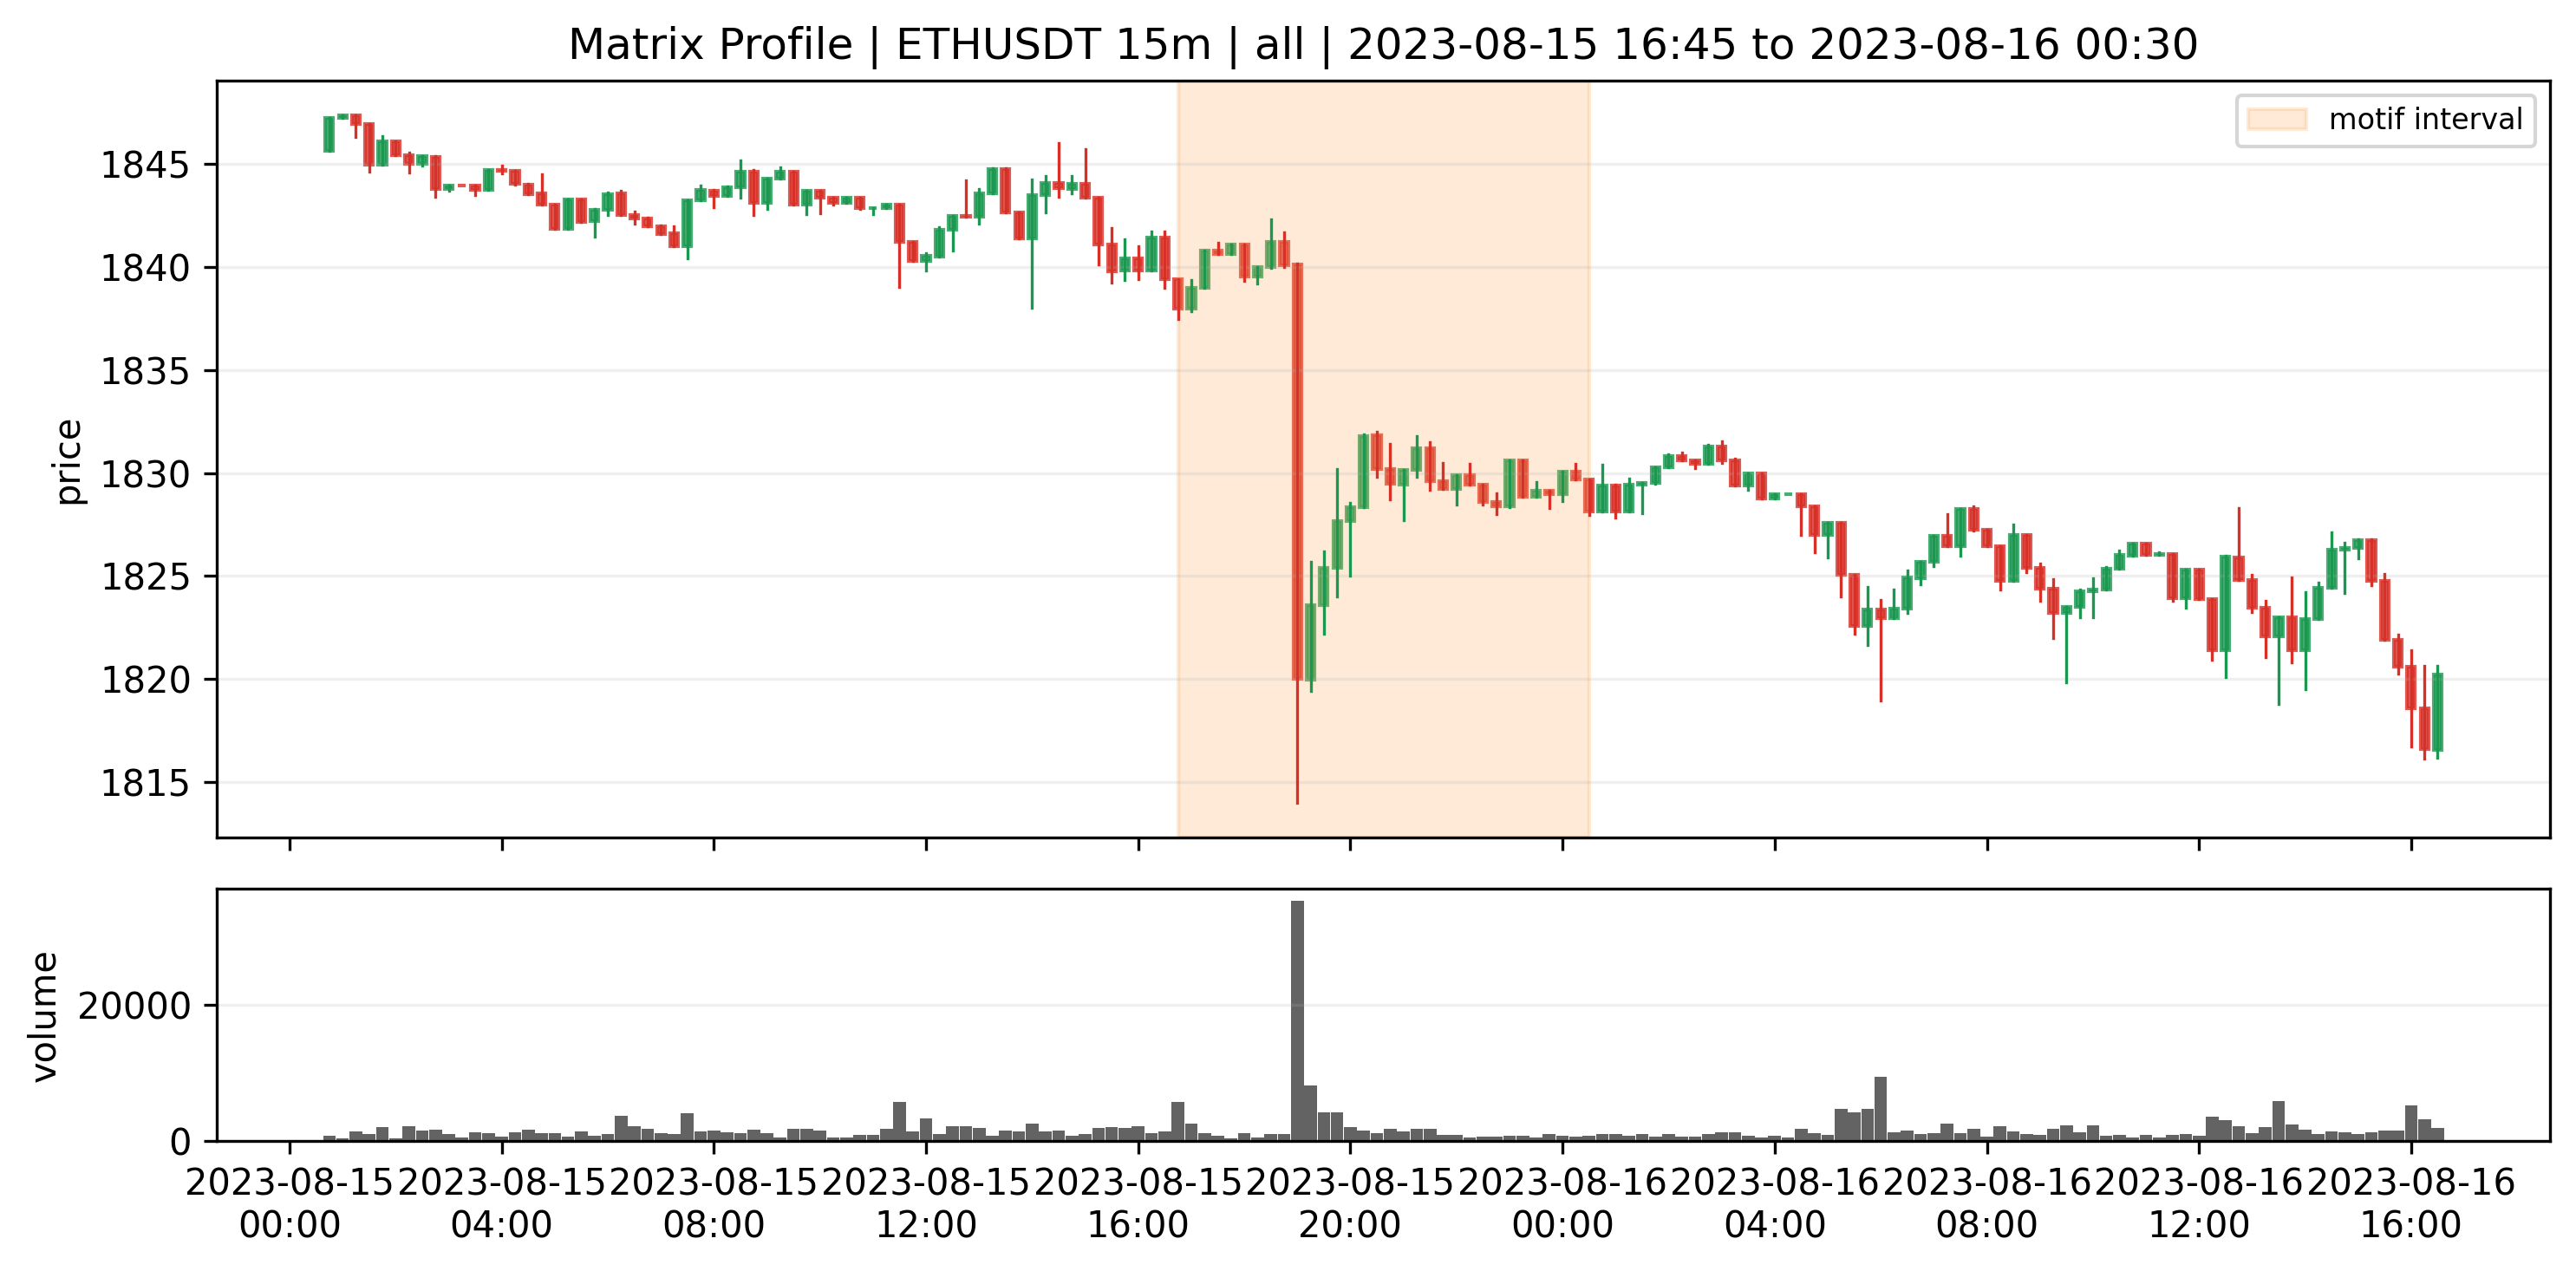
\includegraphics[width=0.9\linewidth]{reports/final_visual_evidence/figures/motif_25_matrix_profile_ethusdt_15m_all_1_0_pair20_1_context.png}
\caption{motif 25 matrix profile ethusdt 15m all 1 0 pair20 1 context. The shaded interval marks the discovered motif occurrence in original price context.}
\end{figure}

\begin{figure}[ht]
\centering
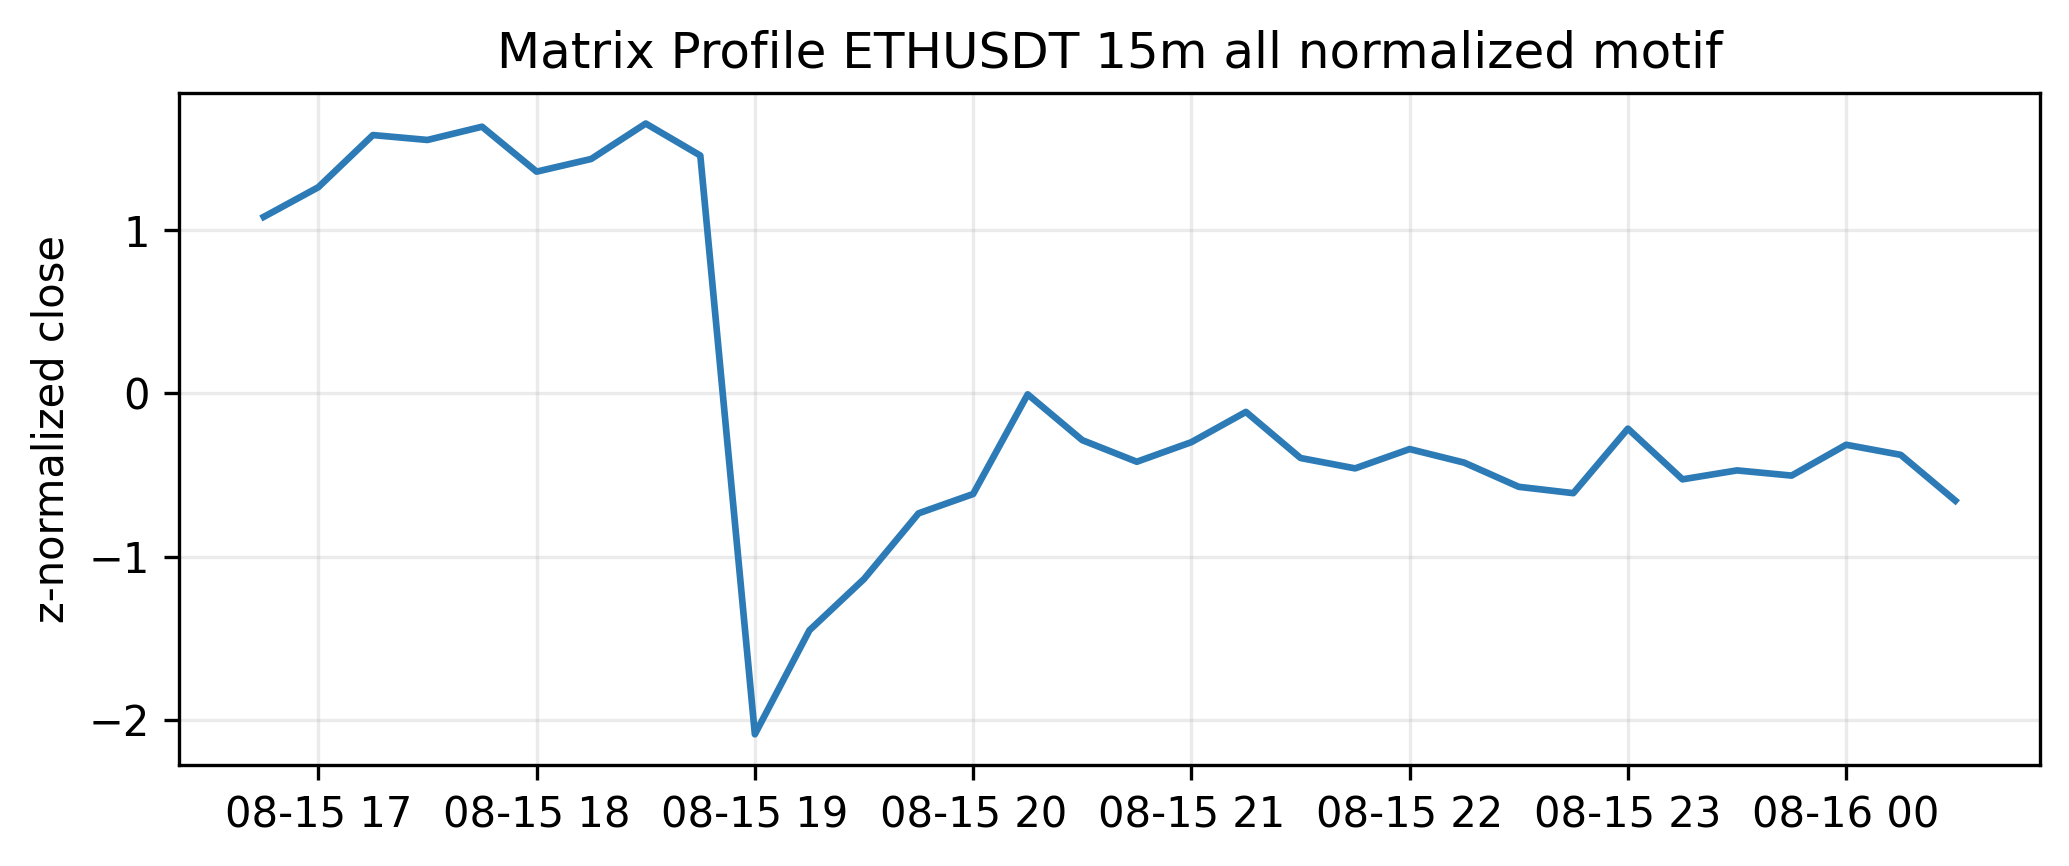
\includegraphics[width=0.9\linewidth]{reports/final_visual_evidence/figures/motif_25_matrix_profile_ethusdt_15m_all_1_0_pair20_1_normal_pattern.png}
\caption{motif 25 matrix profile ethusdt 15m all 1 0 pair20 1 normal pattern. The shaded interval marks the discovered motif occurrence in original price context.}
\end{figure}

\begin{figure}[ht]
\centering
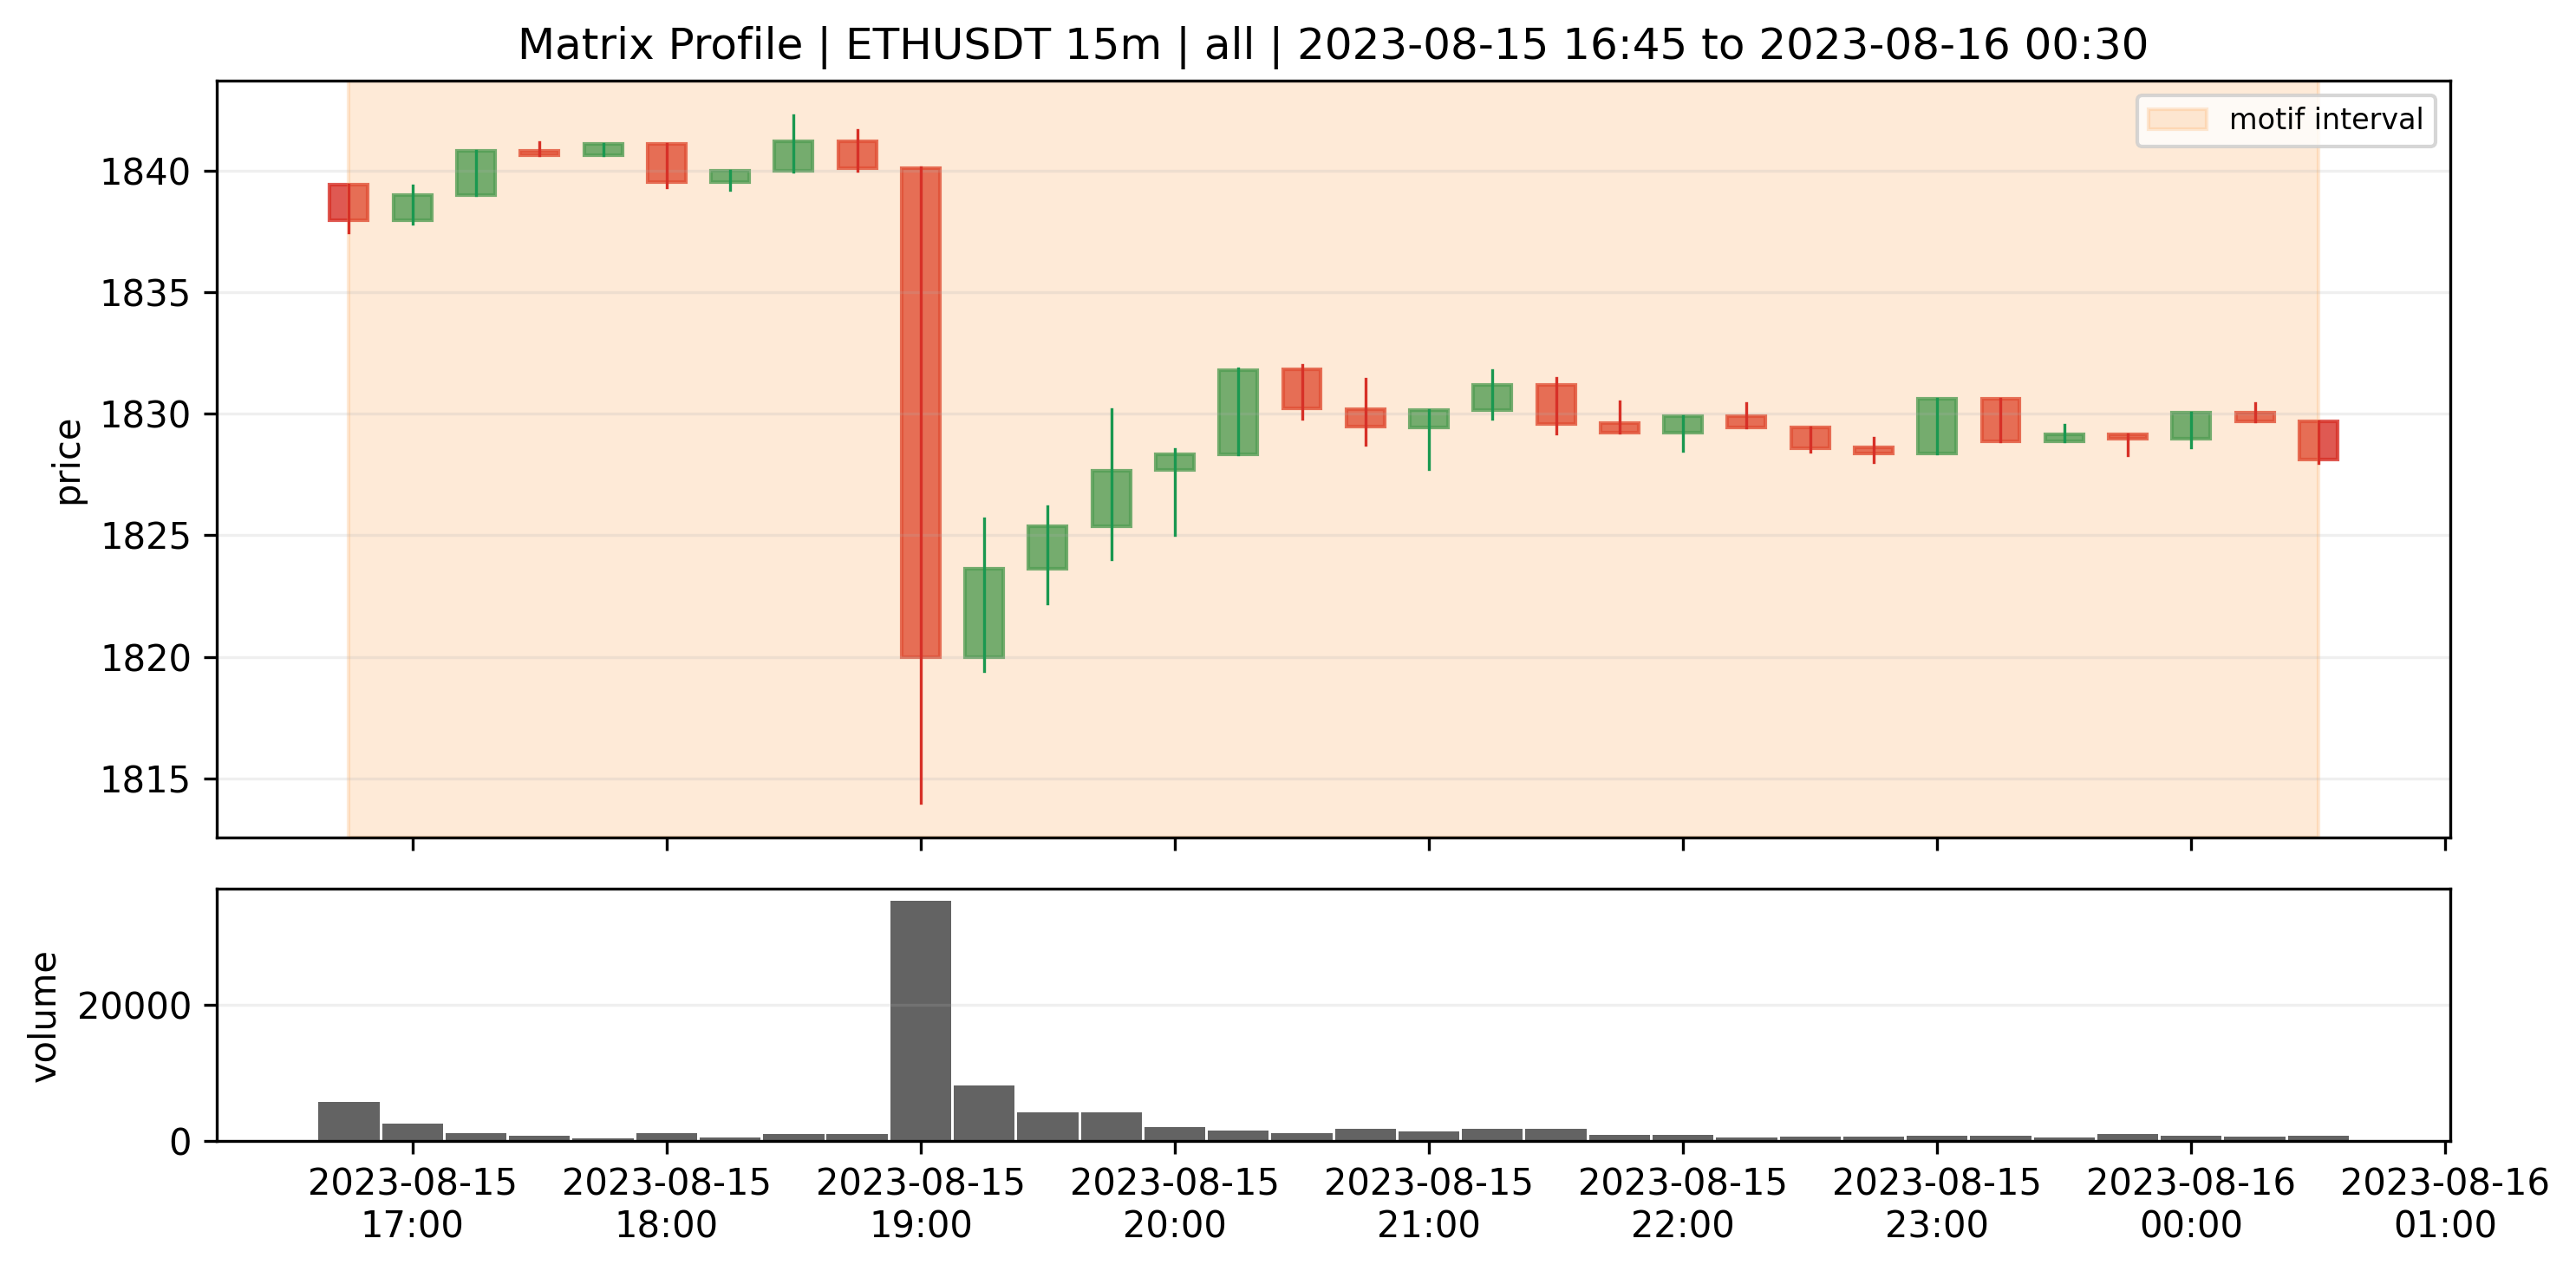
\includegraphics[width=0.9\linewidth]{reports/final_visual_evidence/figures/motif_25_matrix_profile_ethusdt_15m_all_1_0_pair20_1_zoom.png}
\caption{motif 25 matrix profile ethusdt 15m all 1 0 pair20 1 zoom. The shaded interval marks the discovered motif occurrence in original price context.}
\end{figure}

\begin{figure}[ht]
\centering
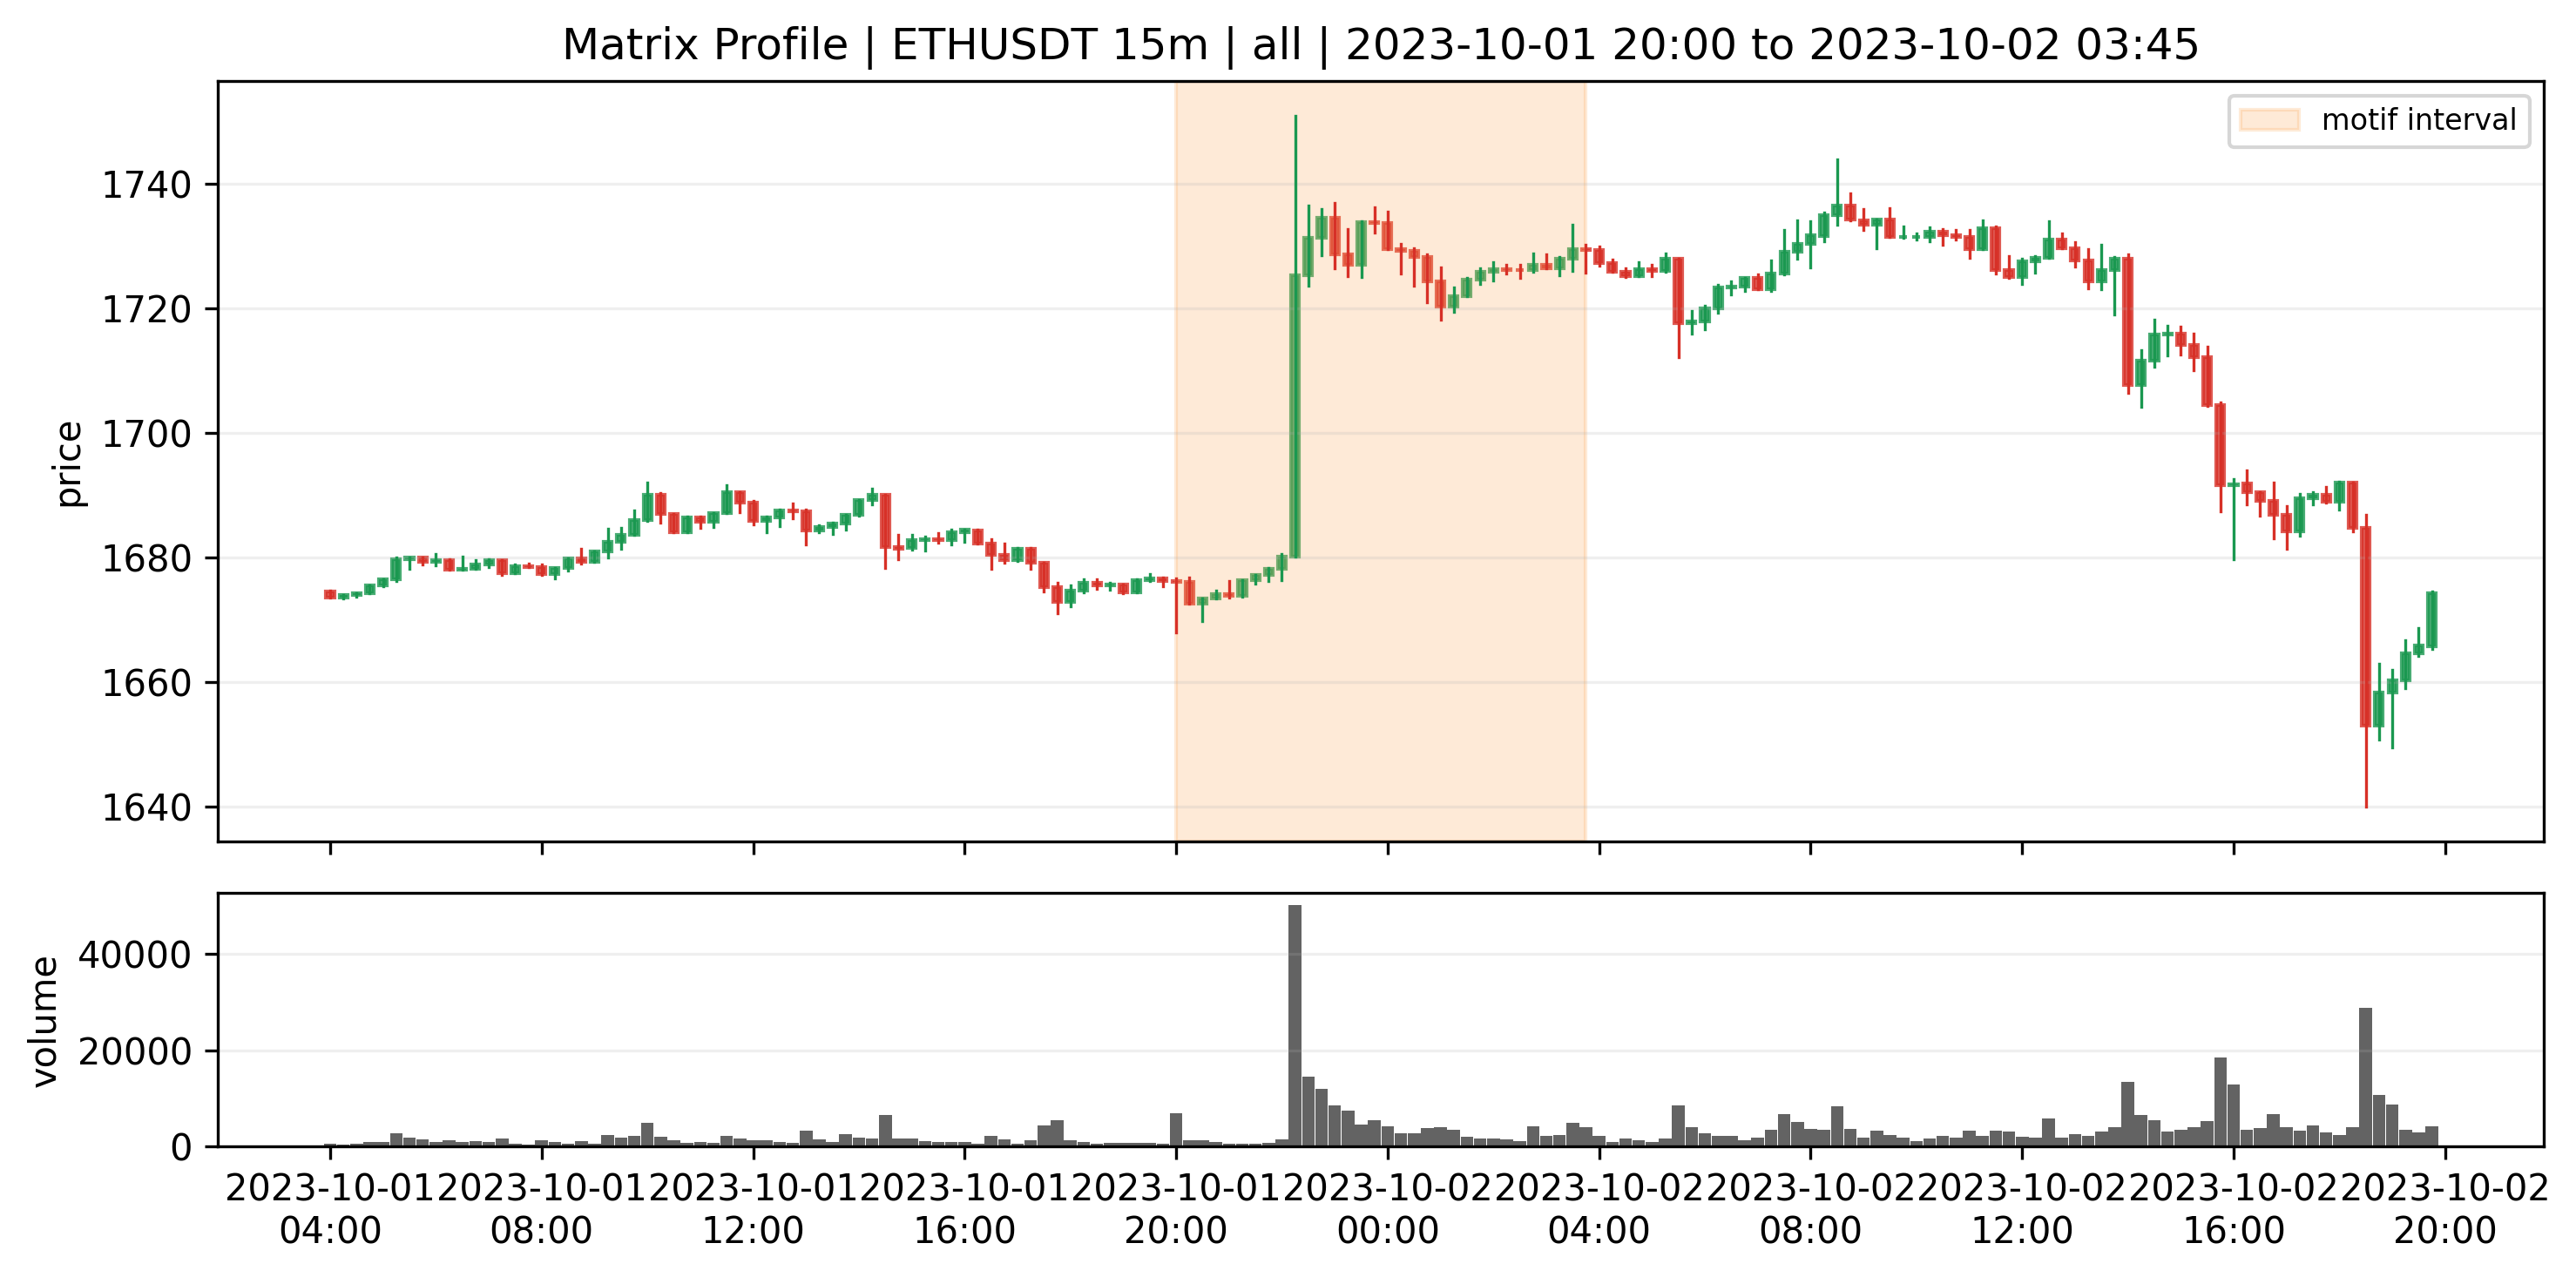
\includegraphics[width=0.9\linewidth]{reports/final_visual_evidence/figures/motif_26_matrix_profile_ethusdt_15m_all_1_0_pair20_2_context.png}
\caption{motif 26 matrix profile ethusdt 15m all 1 0 pair20 2 context. The shaded interval marks the discovered motif occurrence in original price context.}
\end{figure}

\begin{figure}[ht]
\centering
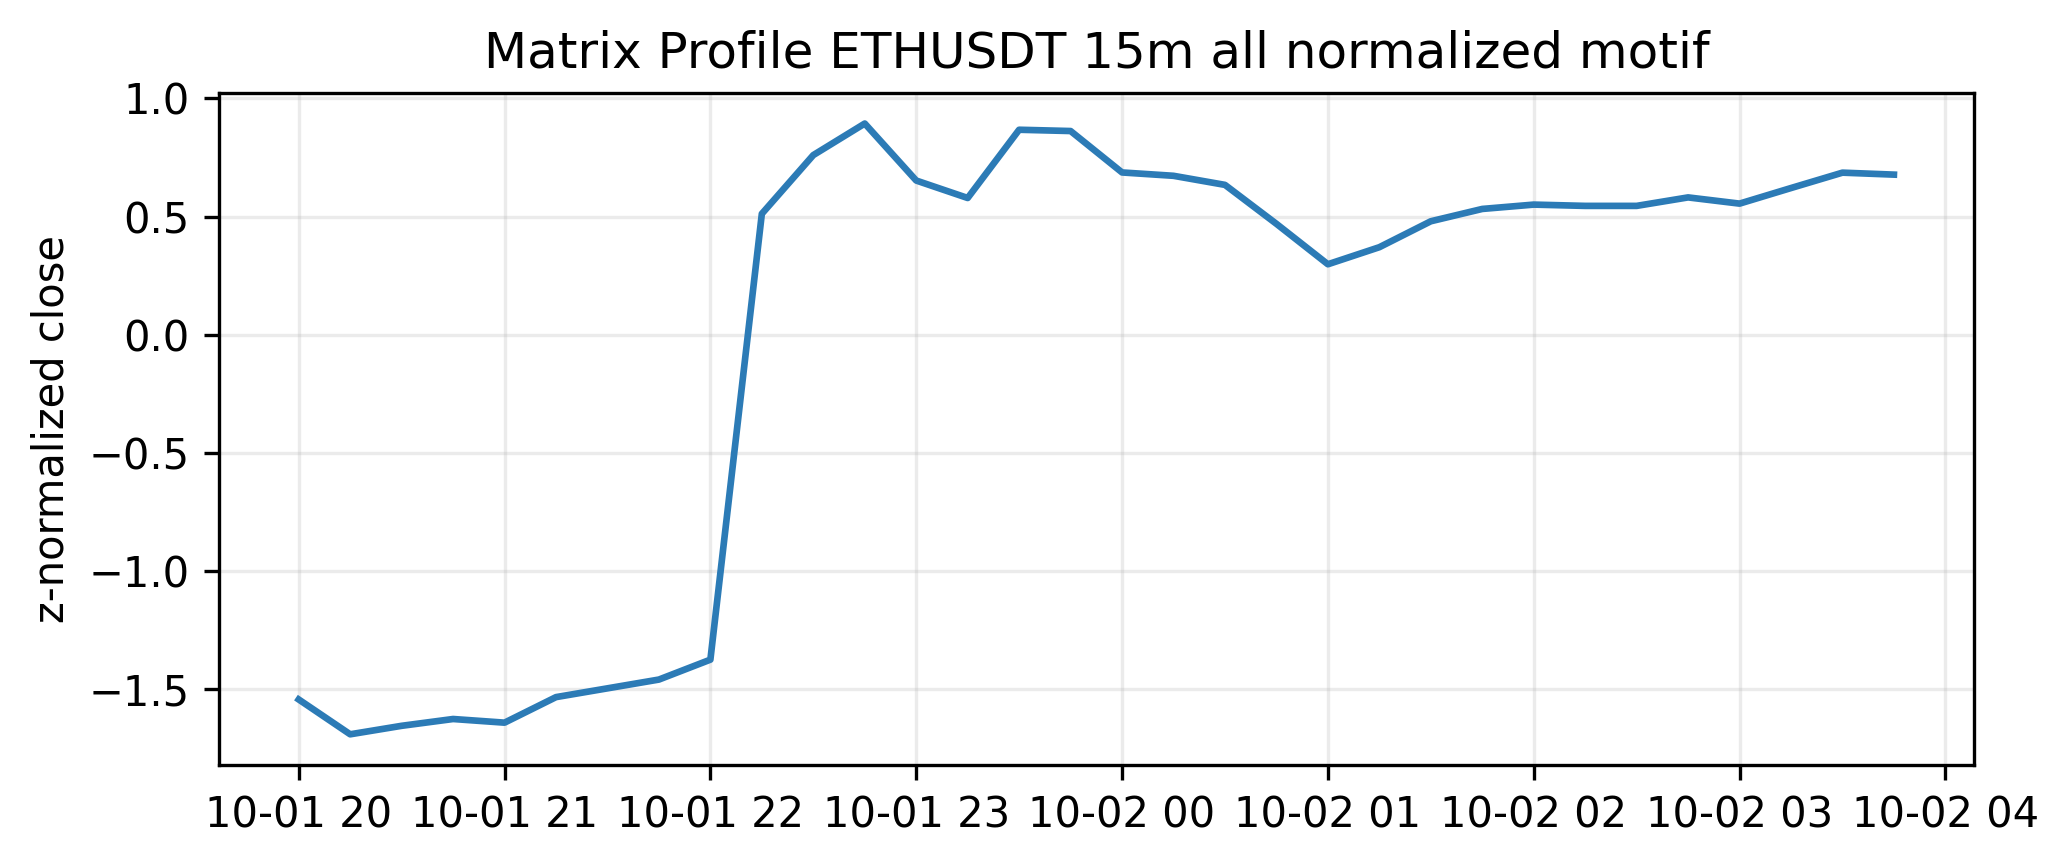
\includegraphics[width=0.9\linewidth]{reports/final_visual_evidence/figures/motif_26_matrix_profile_ethusdt_15m_all_1_0_pair20_2_normal_pattern.png}
\caption{motif 26 matrix profile ethusdt 15m all 1 0 pair20 2 normal pattern. The shaded interval marks the discovered motif occurrence in original price context.}
\end{figure}

\begin{figure}[ht]
\centering
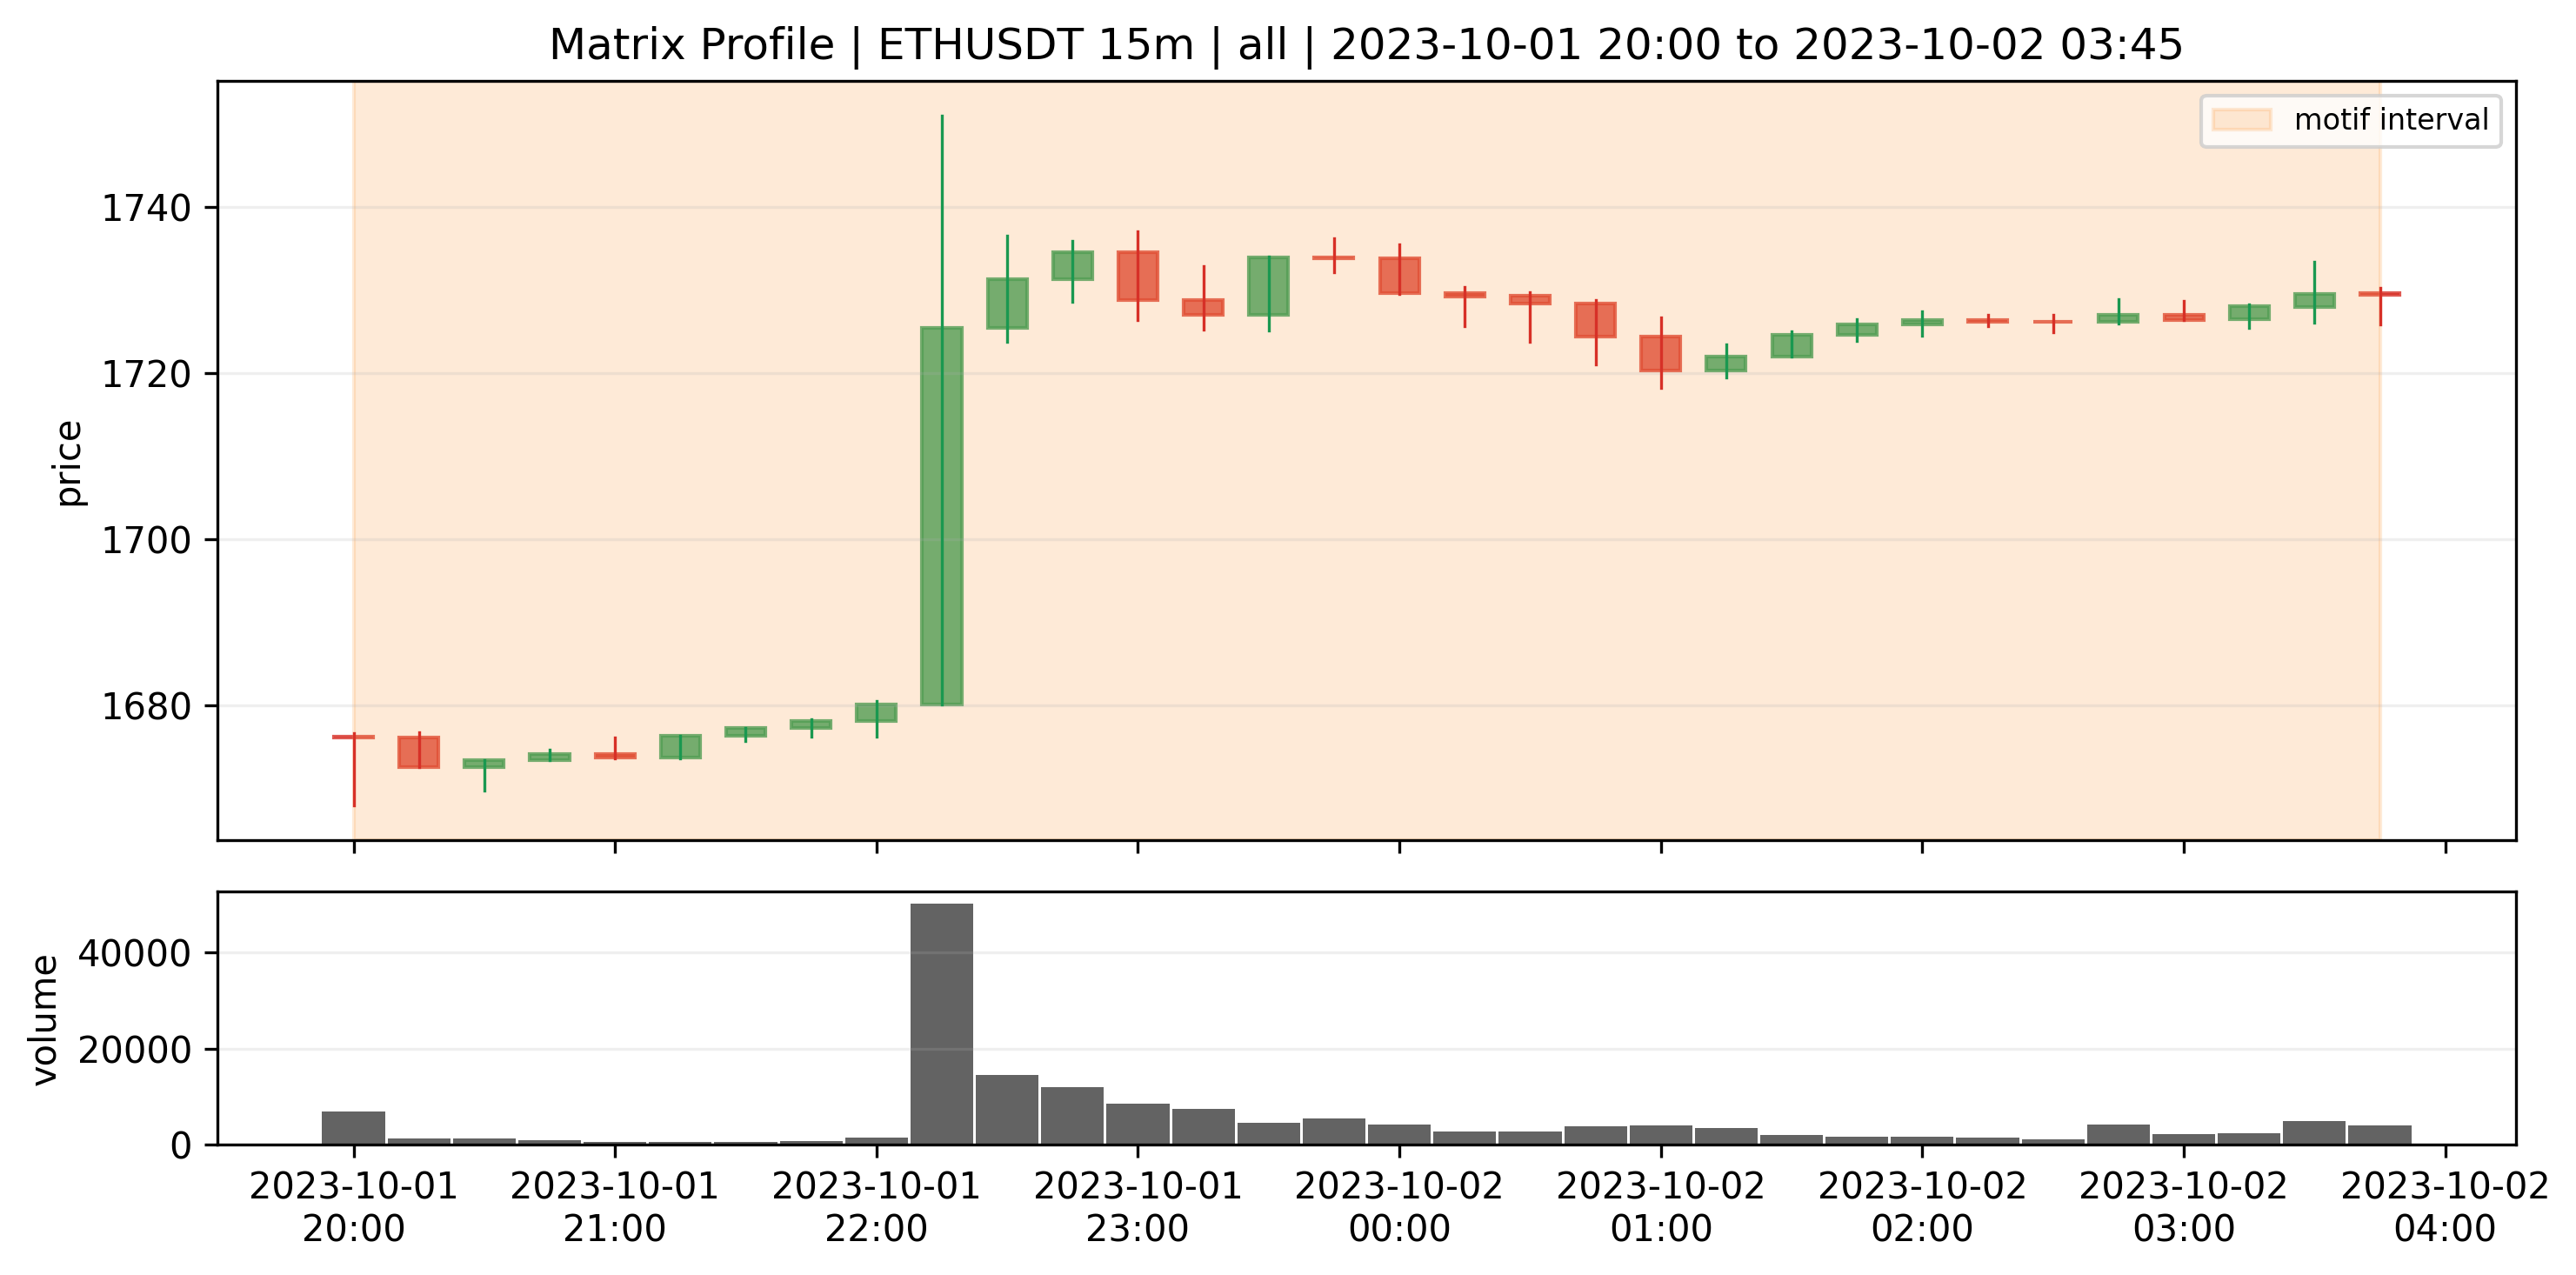
\includegraphics[width=0.9\linewidth]{reports/final_visual_evidence/figures/motif_26_matrix_profile_ethusdt_15m_all_1_0_pair20_2_zoom.png}
\caption{motif 26 matrix profile ethusdt 15m all 1 0 pair20 2 zoom. The shaded interval marks the discovered motif occurrence in original price context.}
\end{figure}

\begin{figure}[ht]
\centering
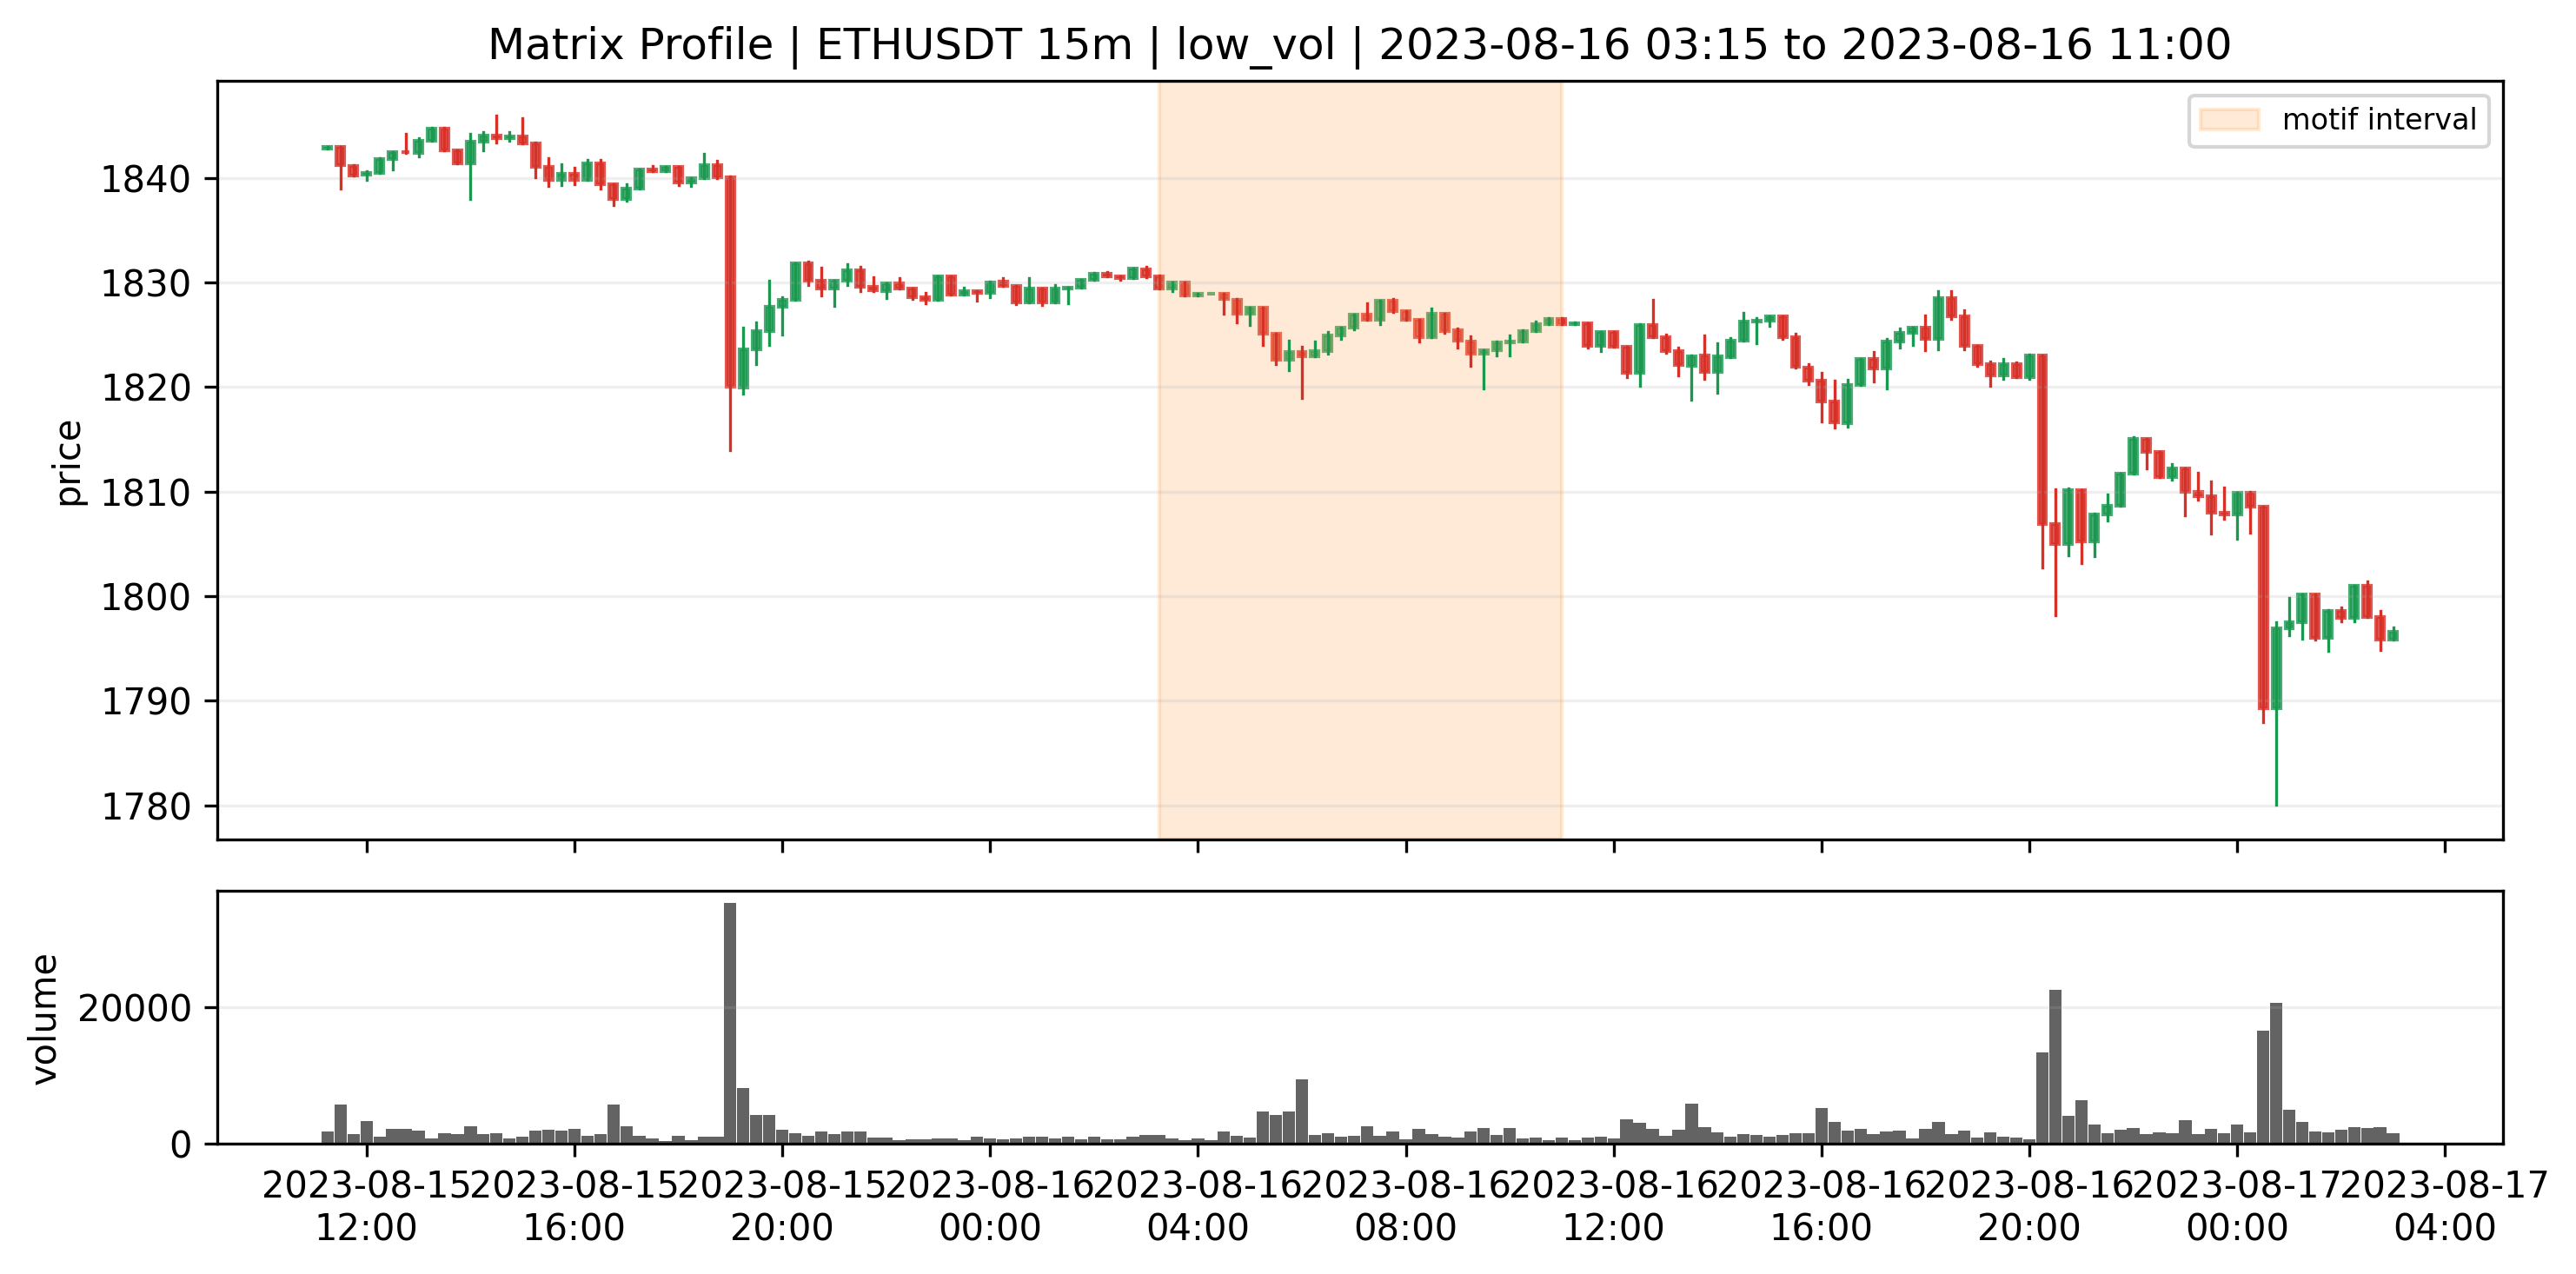
\includegraphics[width=0.9\linewidth]{reports/final_visual_evidence/figures/motif_27_matrix_profile_ethusdt_15m_low_vol_1_0_pair39_1_context.png}
\caption{motif 27 matrix profile ethusdt 15m low vol 1 0 pair39 1 context. The shaded interval marks the discovered motif occurrence in original price context.}
\end{figure}

\begin{figure}[ht]
\centering
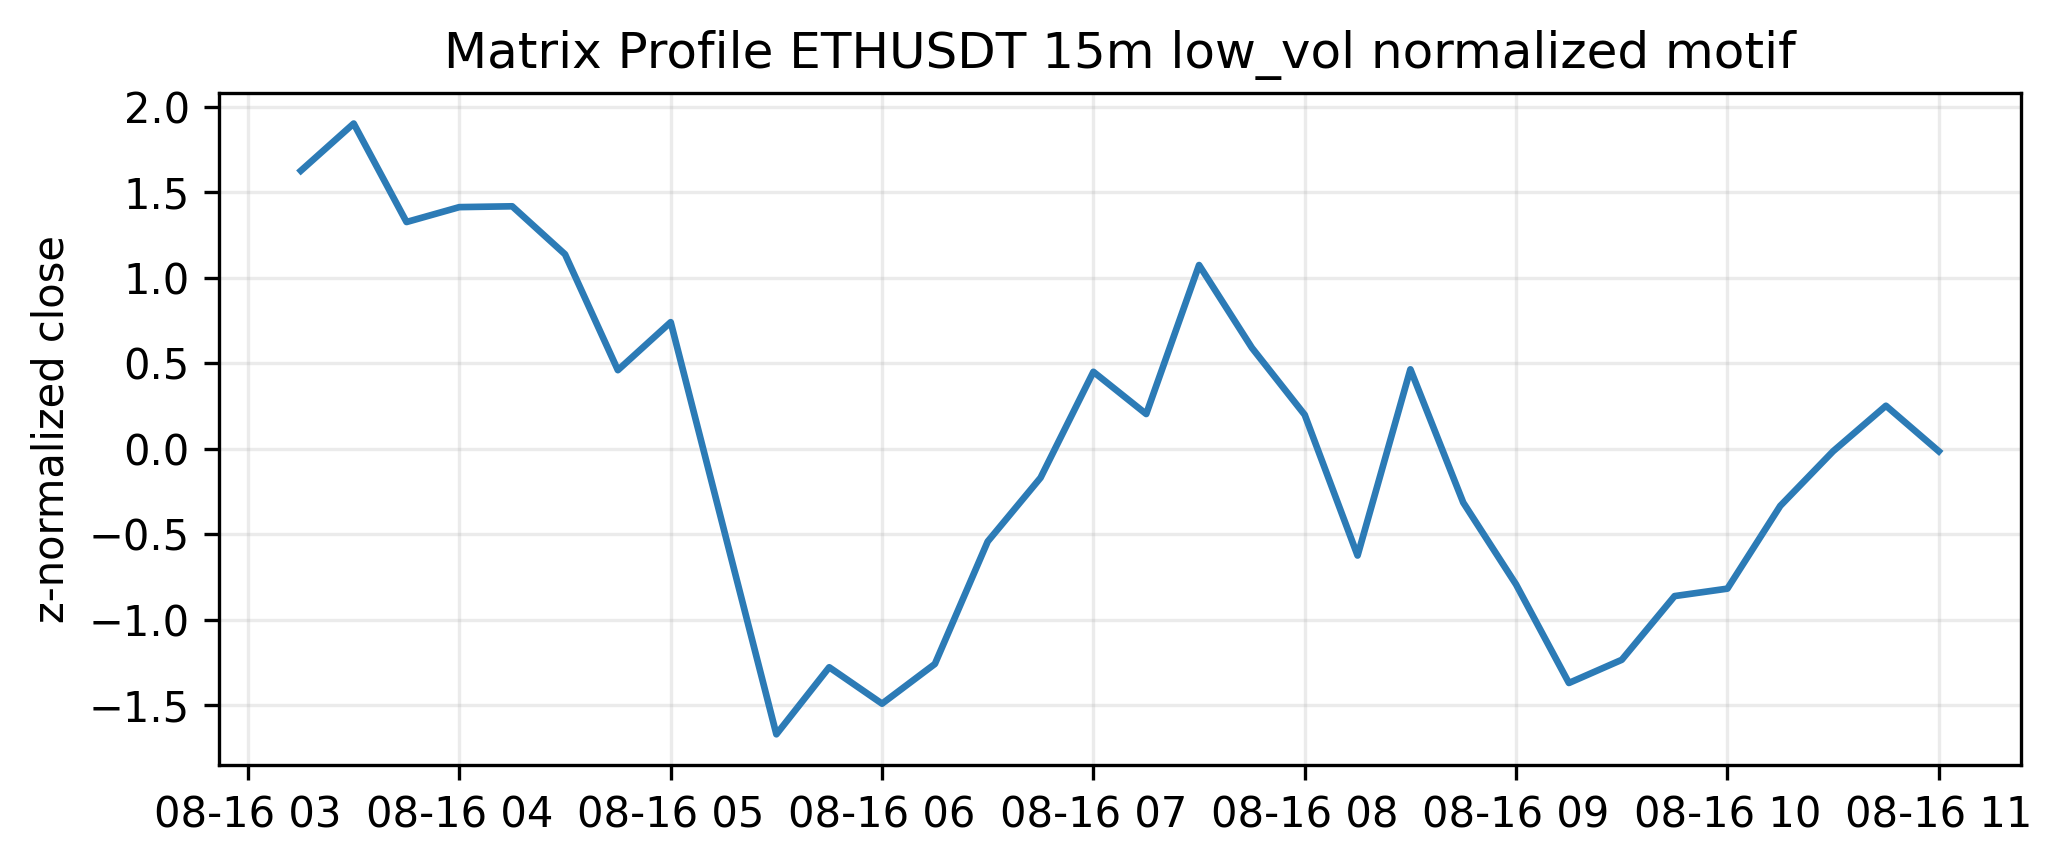
\includegraphics[width=0.9\linewidth]{reports/final_visual_evidence/figures/motif_27_matrix_profile_ethusdt_15m_low_vol_1_0_pair39_1_normal_pattern.png}
\caption{motif 27 matrix profile ethusdt 15m low vol 1 0 pair39 1 normal pattern. The shaded interval marks the discovered motif occurrence in original price context.}
\end{figure}

\begin{figure}[ht]
\centering
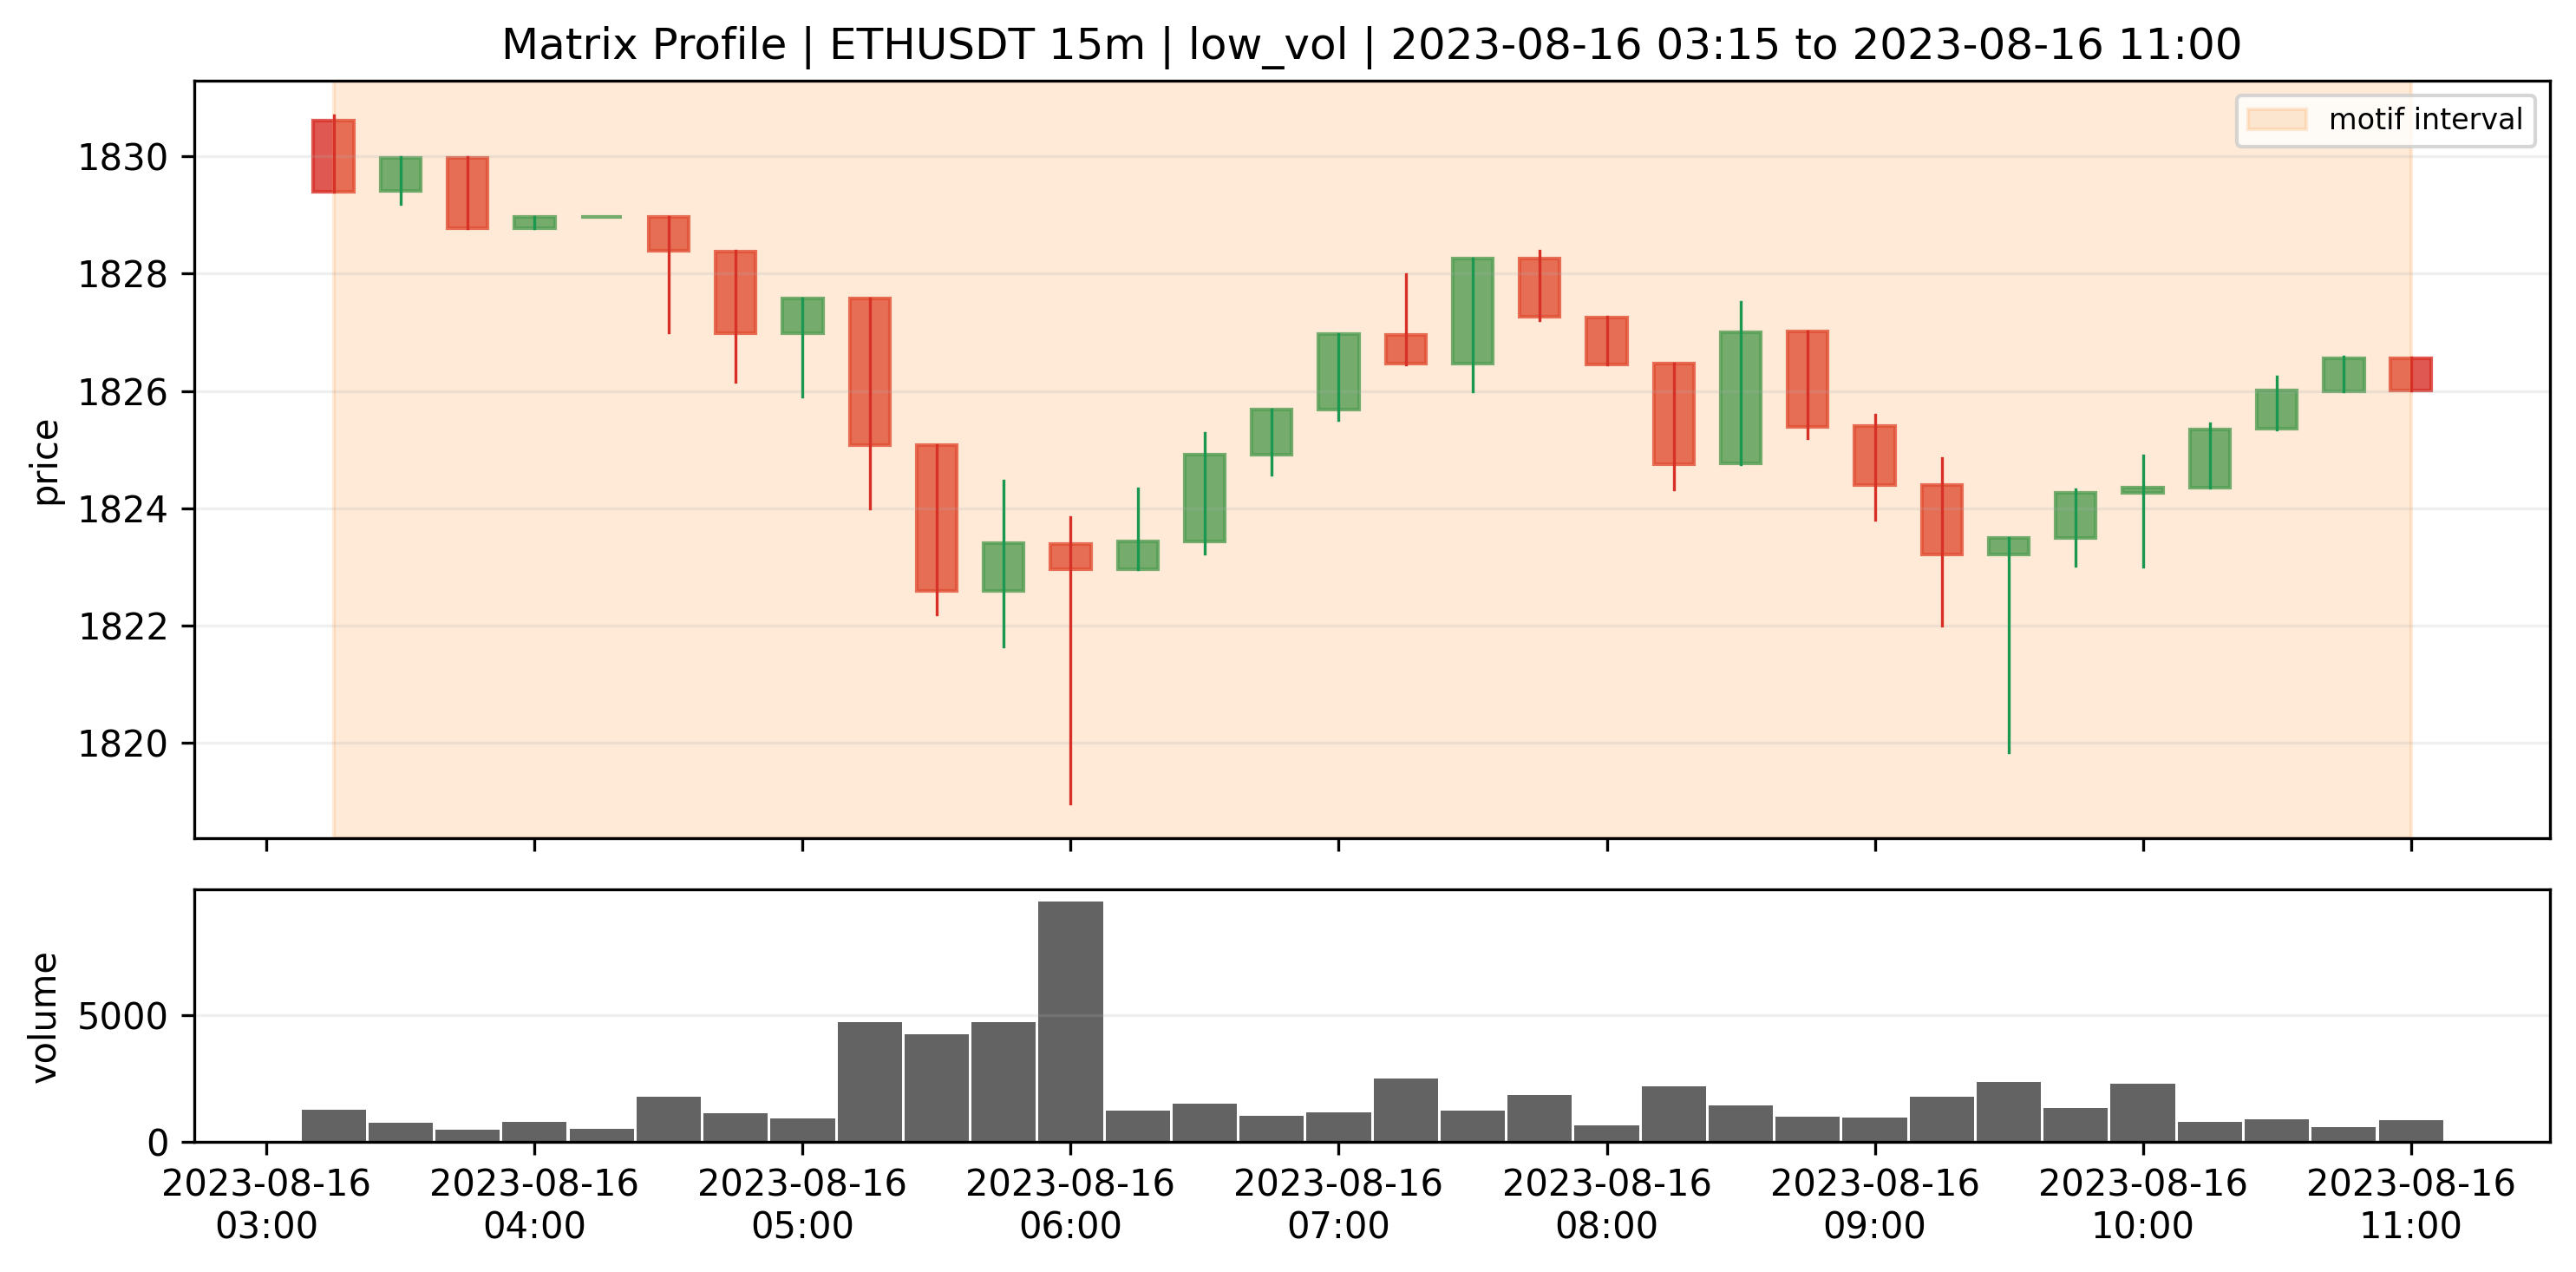
\includegraphics[width=0.9\linewidth]{reports/final_visual_evidence/figures/motif_27_matrix_profile_ethusdt_15m_low_vol_1_0_pair39_1_zoom.png}
\caption{motif 27 matrix profile ethusdt 15m low vol 1 0 pair39 1 zoom. The shaded interval marks the discovered motif occurrence in original price context.}
\end{figure}

\begin{figure}[ht]
\centering
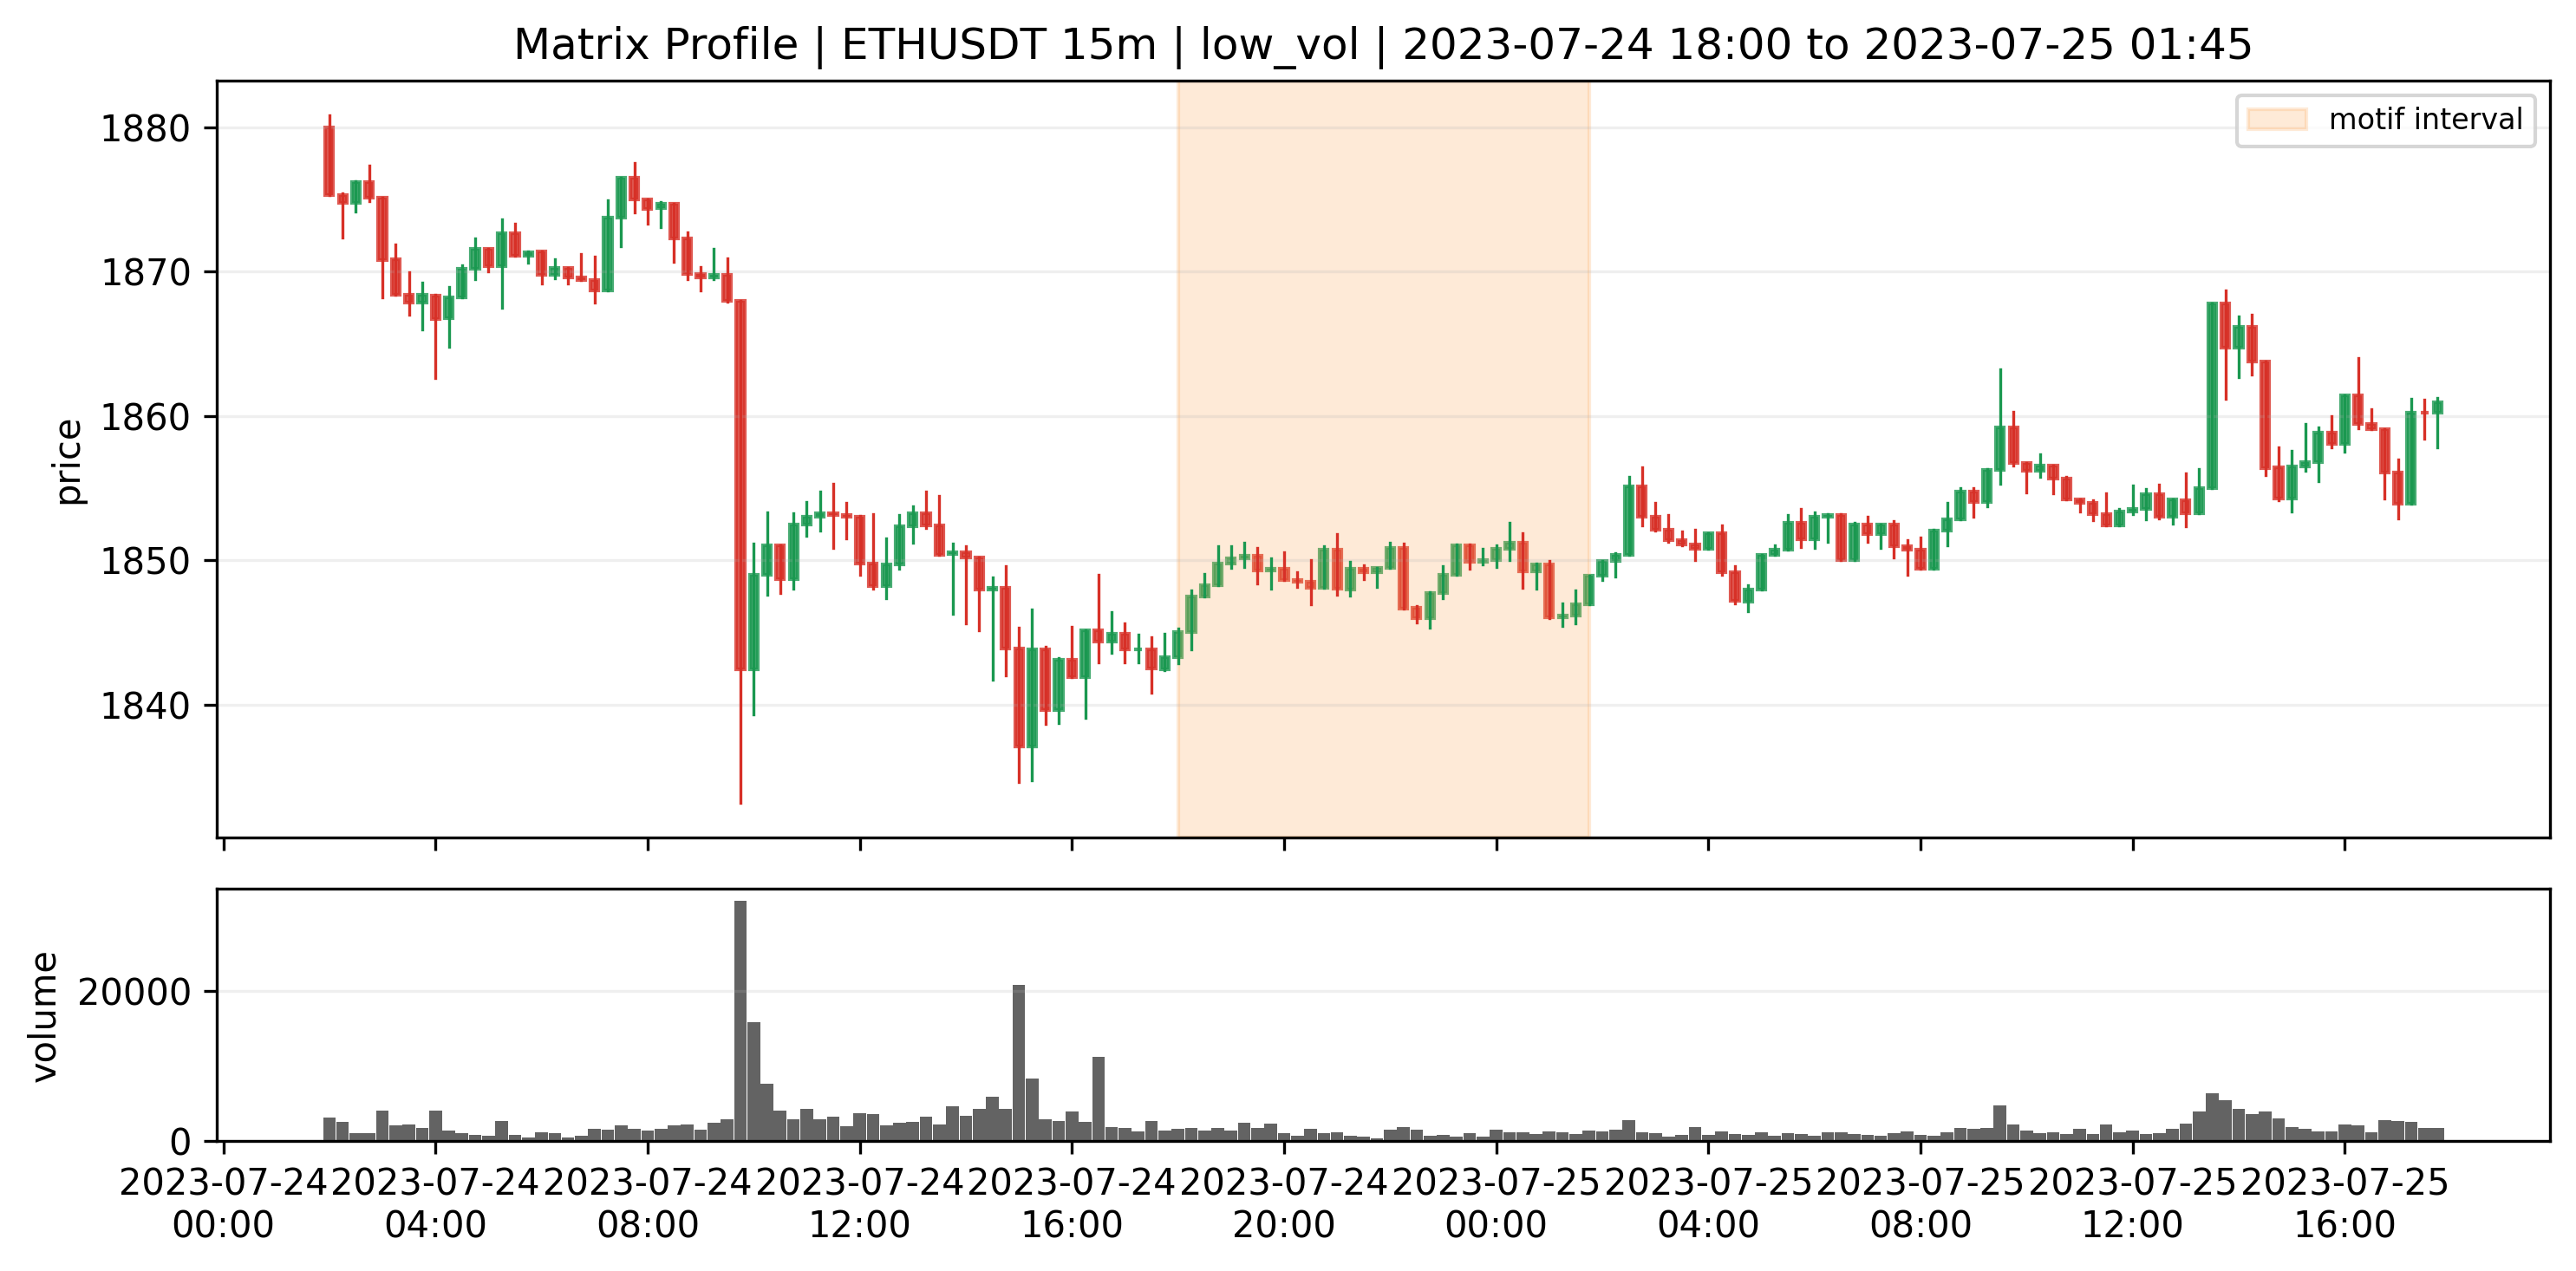
\includegraphics[width=0.9\linewidth]{reports/final_visual_evidence/figures/motif_28_matrix_profile_ethusdt_15m_low_vol_1_0_pair39_2_context.png}
\caption{motif 28 matrix profile ethusdt 15m low vol 1 0 pair39 2 context. The shaded interval marks the discovered motif occurrence in original price context.}
\end{figure}

\begin{figure}[ht]
\centering
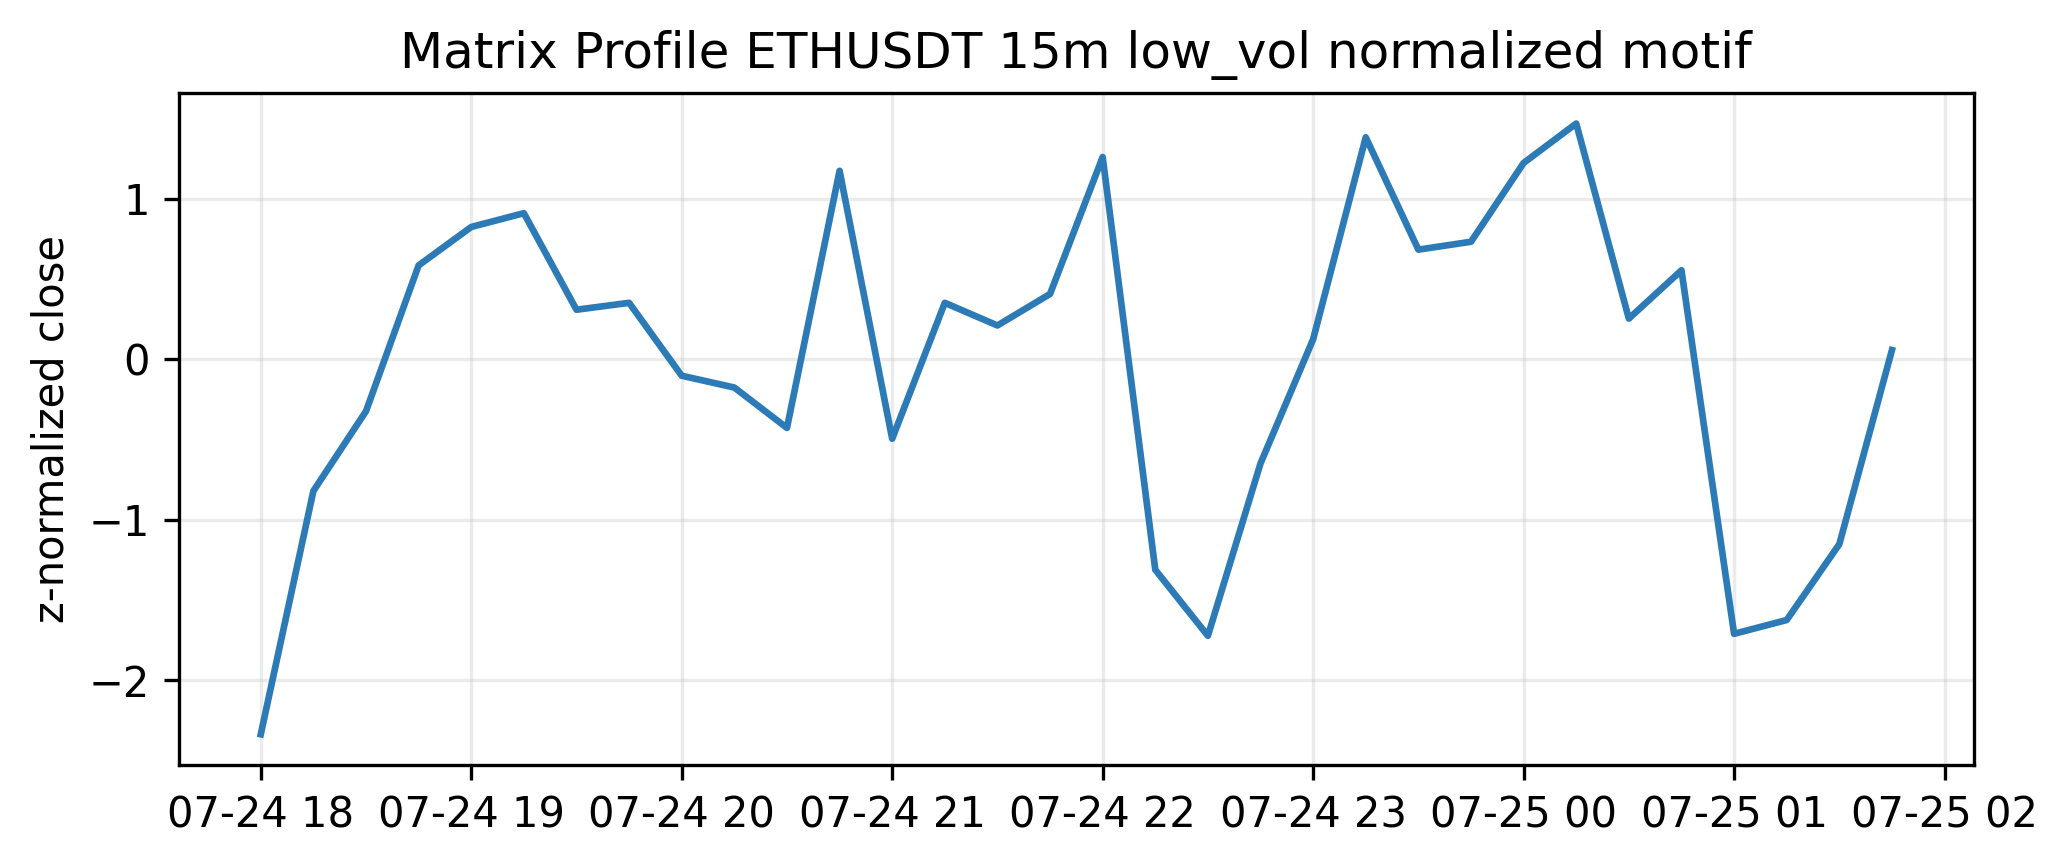
\includegraphics[width=0.9\linewidth]{reports/final_visual_evidence/figures/motif_28_matrix_profile_ethusdt_15m_low_vol_1_0_pair39_2_normal_pattern.png}
\caption{motif 28 matrix profile ethusdt 15m low vol 1 0 pair39 2 normal pattern. The shaded interval marks the discovered motif occurrence in original price context.}
\end{figure}

\begin{figure}[ht]
\centering
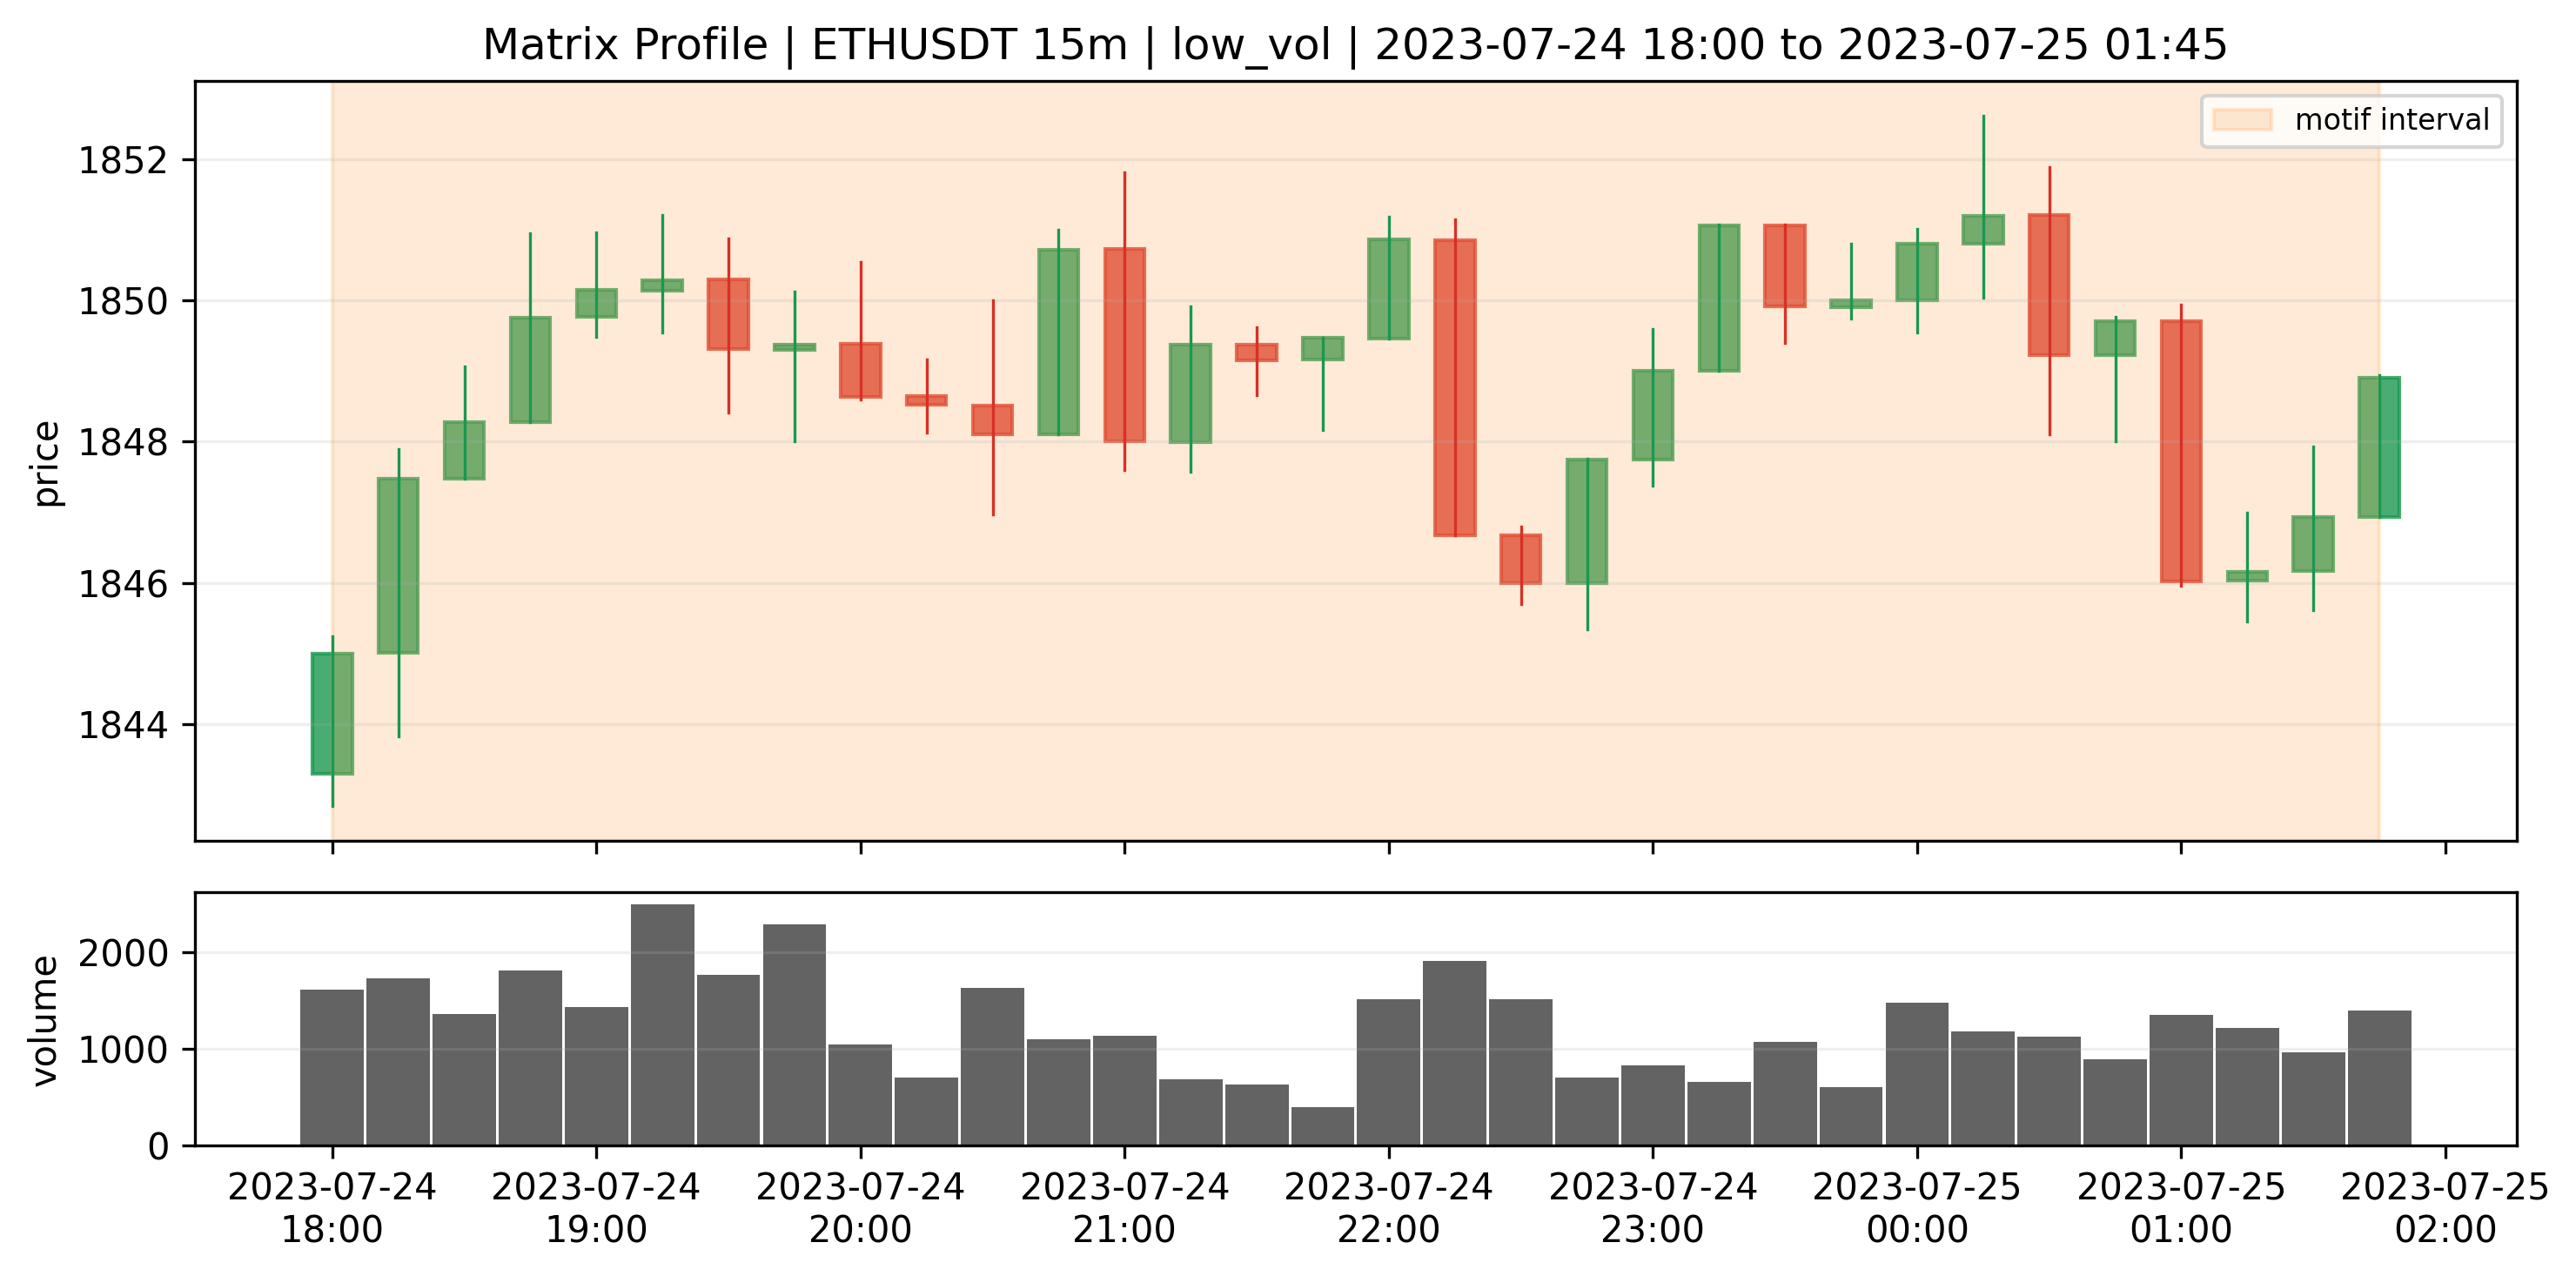
\includegraphics[width=0.9\linewidth]{reports/final_visual_evidence/figures/motif_28_matrix_profile_ethusdt_15m_low_vol_1_0_pair39_2_zoom.png}
\caption{motif 28 matrix profile ethusdt 15m low vol 1 0 pair39 2 zoom. The shaded interval marks the discovered motif occurrence in original price context.}
\end{figure}

\begin{figure}[ht]
\centering
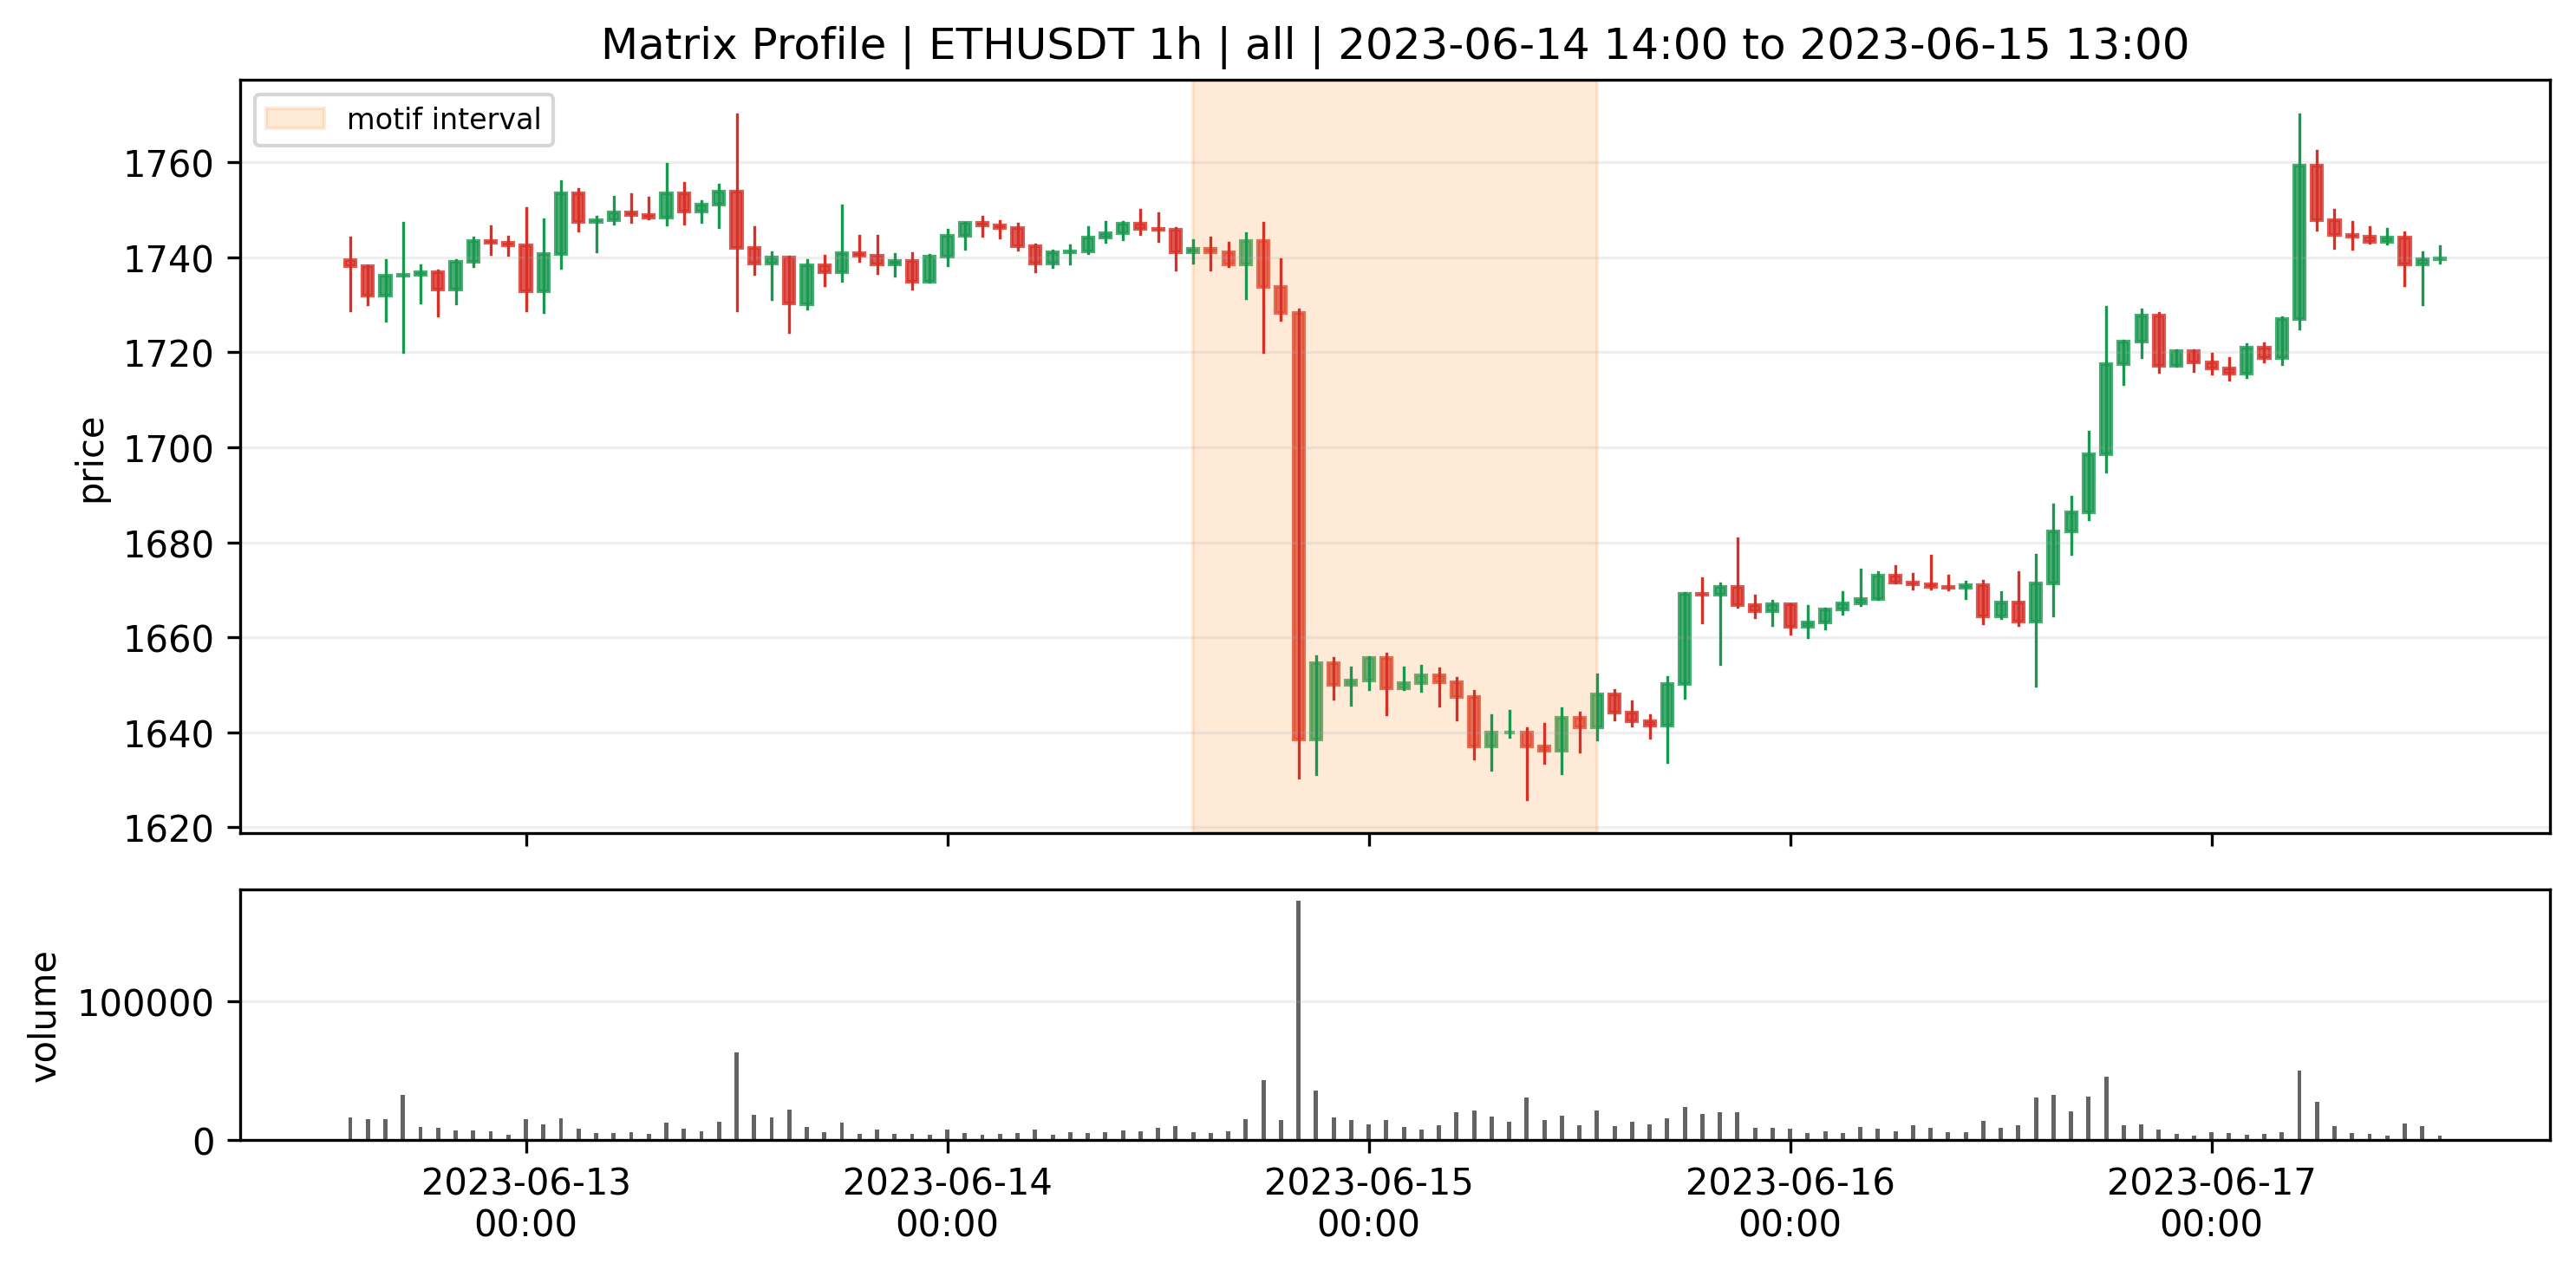
\includegraphics[width=0.9\linewidth]{reports/final_visual_evidence/figures/motif_29_matrix_profile_ethusdt_1h_all_1_0_pair27_1_context.png}
\caption{motif 29 matrix profile ethusdt 1h all 1 0 pair27 1 context. The shaded interval marks the discovered motif occurrence in original price context.}
\end{figure}

\begin{figure}[ht]
\centering
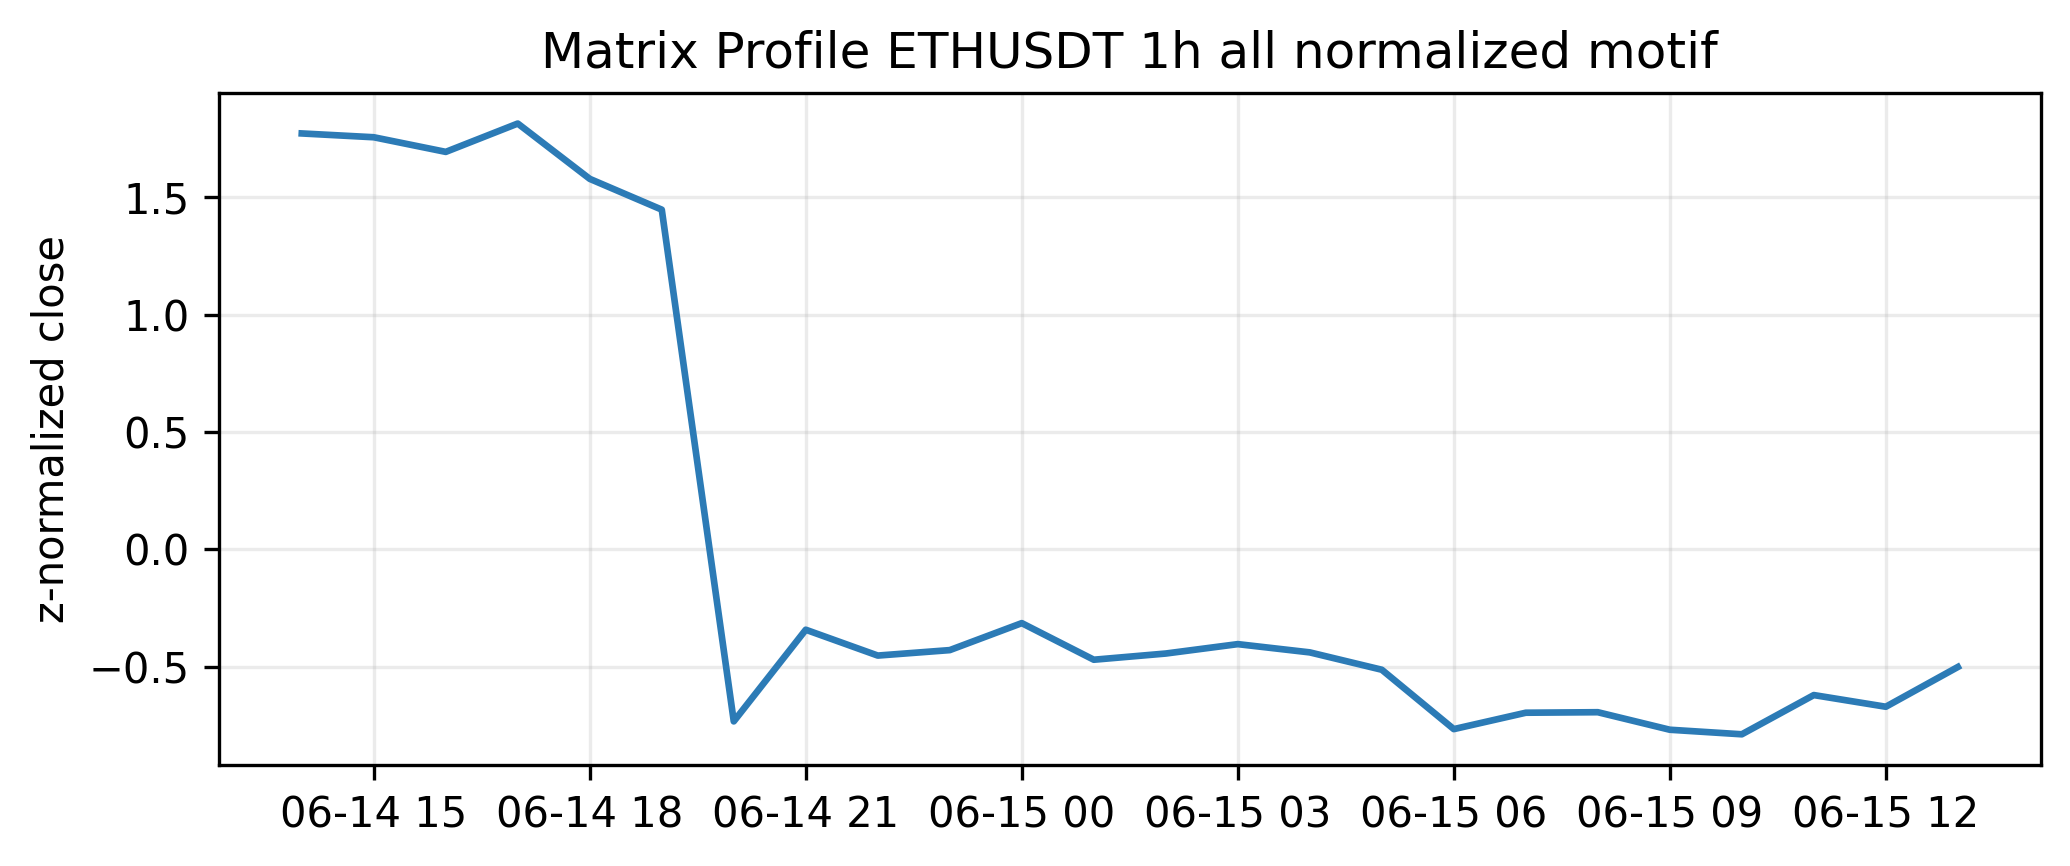
\includegraphics[width=0.9\linewidth]{reports/final_visual_evidence/figures/motif_29_matrix_profile_ethusdt_1h_all_1_0_pair27_1_normal_pattern.png}
\caption{motif 29 matrix profile ethusdt 1h all 1 0 pair27 1 normal pattern. The shaded interval marks the discovered motif occurrence in original price context.}
\end{figure}

\begin{figure}[ht]
\centering
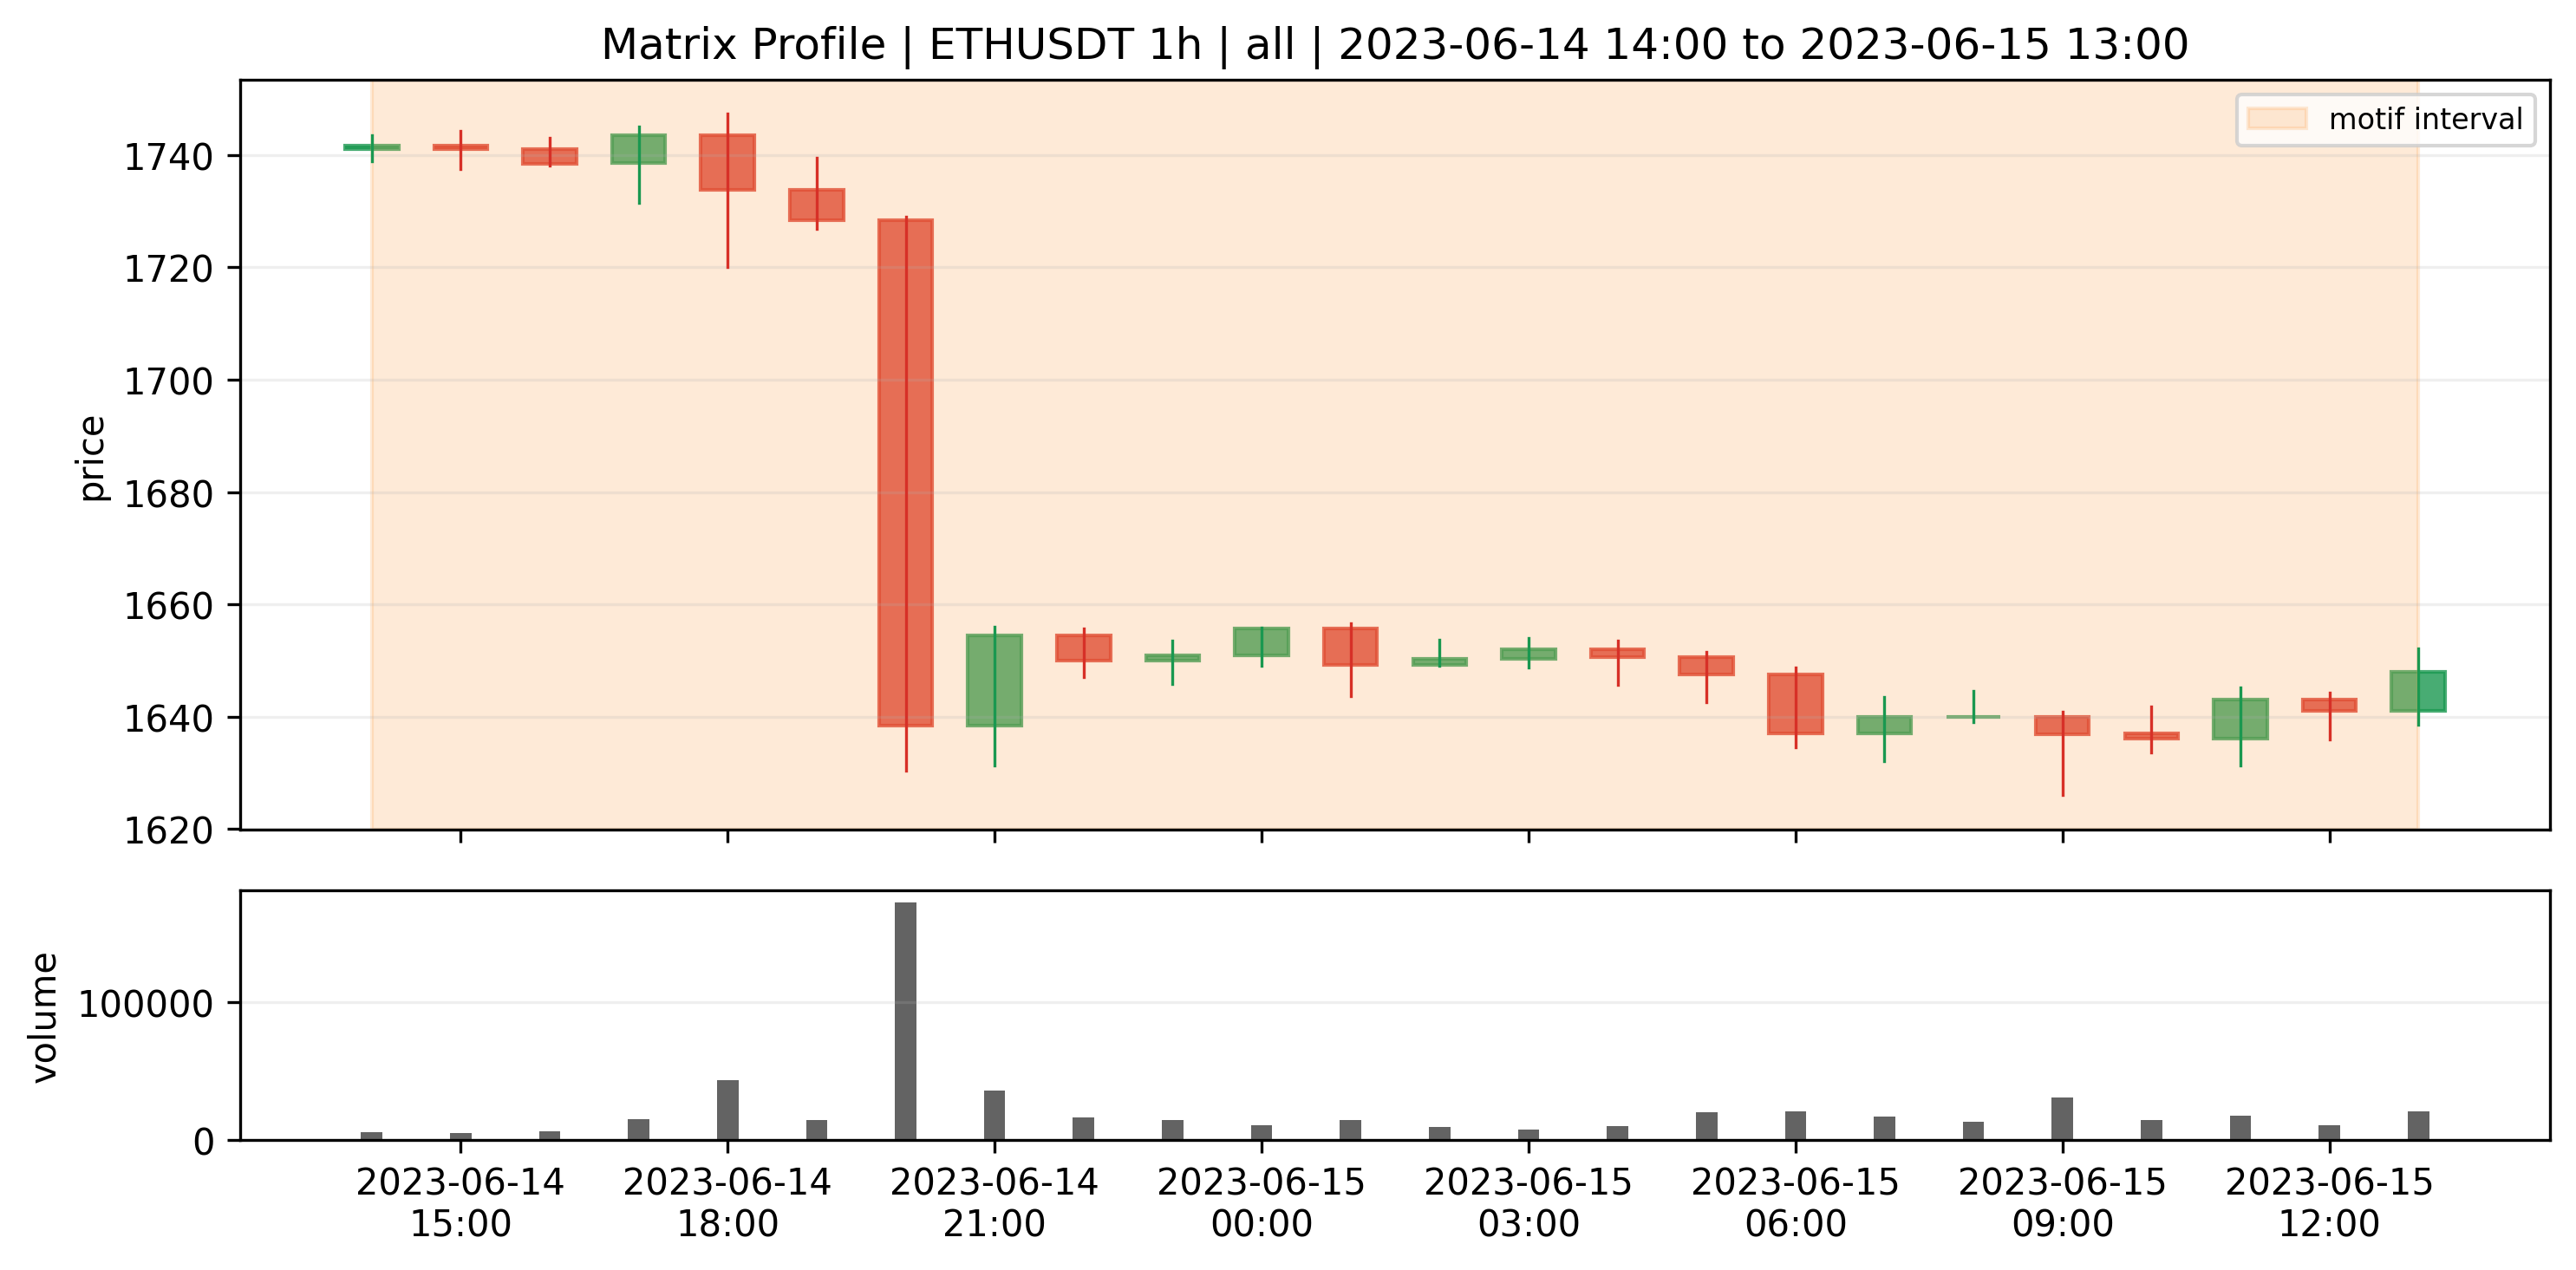
\includegraphics[width=0.9\linewidth]{reports/final_visual_evidence/figures/motif_29_matrix_profile_ethusdt_1h_all_1_0_pair27_1_zoom.png}
\caption{motif 29 matrix profile ethusdt 1h all 1 0 pair27 1 zoom. The shaded interval marks the discovered motif occurrence in original price context.}
\end{figure}

\begin{figure}[ht]
\centering
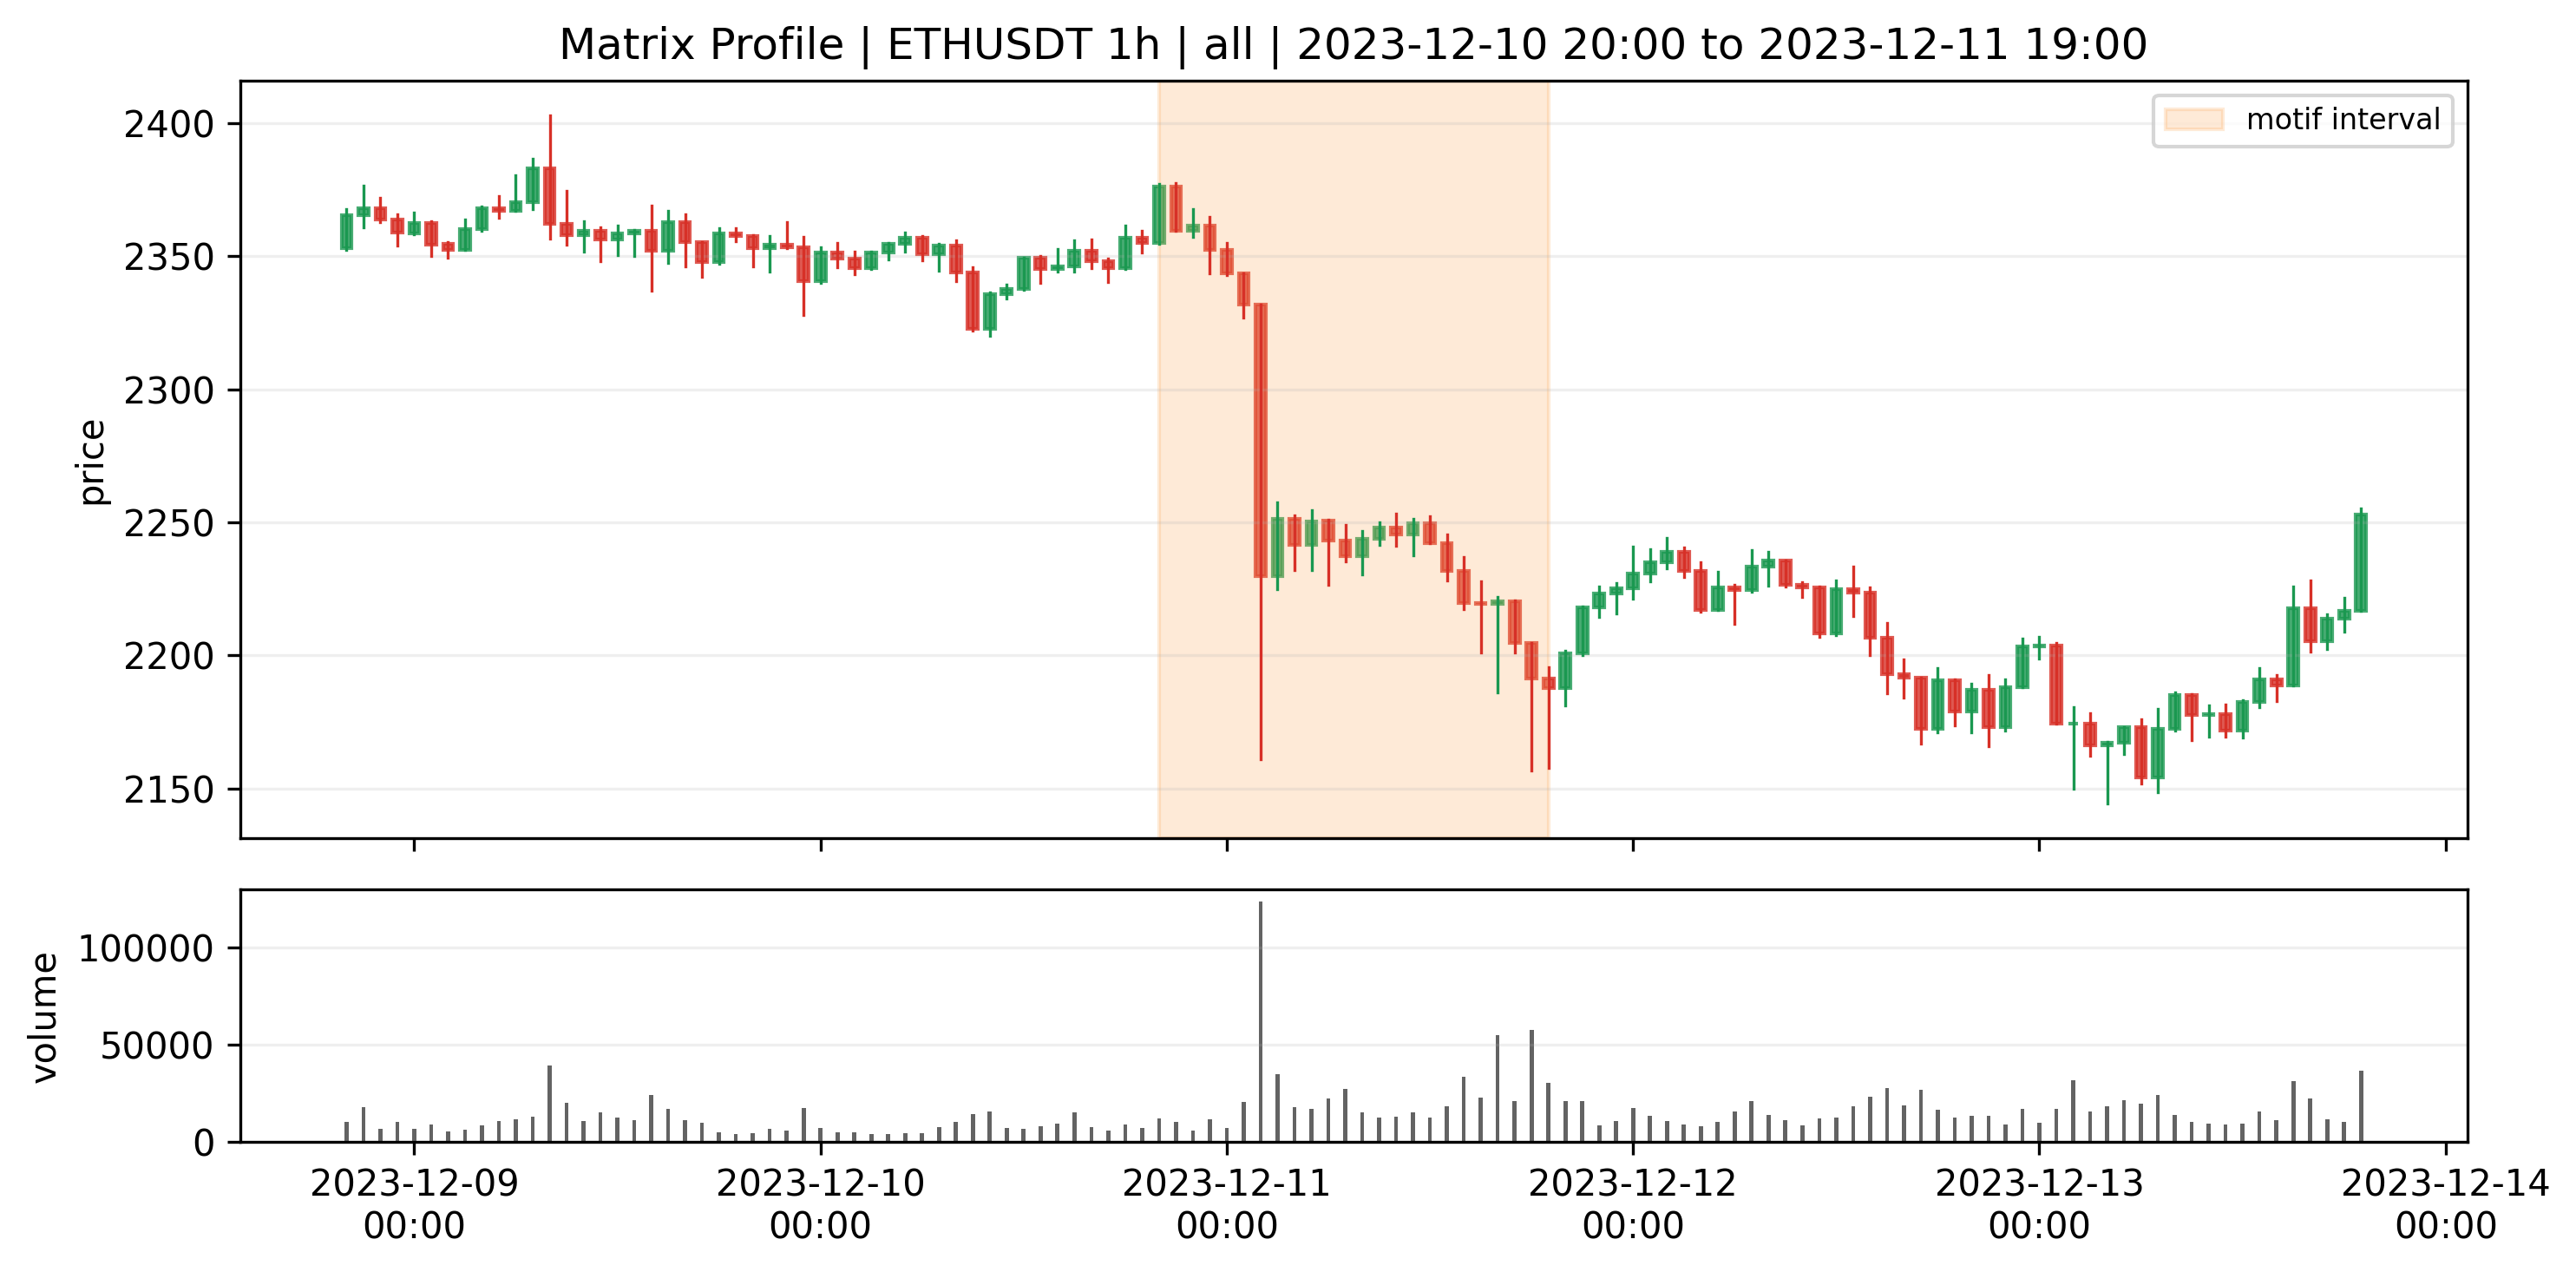
\includegraphics[width=0.9\linewidth]{reports/final_visual_evidence/figures/motif_30_matrix_profile_ethusdt_1h_all_1_0_pair27_2_context.png}
\caption{motif 30 matrix profile ethusdt 1h all 1 0 pair27 2 context. The shaded interval marks the discovered motif occurrence in original price context.}
\end{figure}

\begin{figure}[ht]
\centering
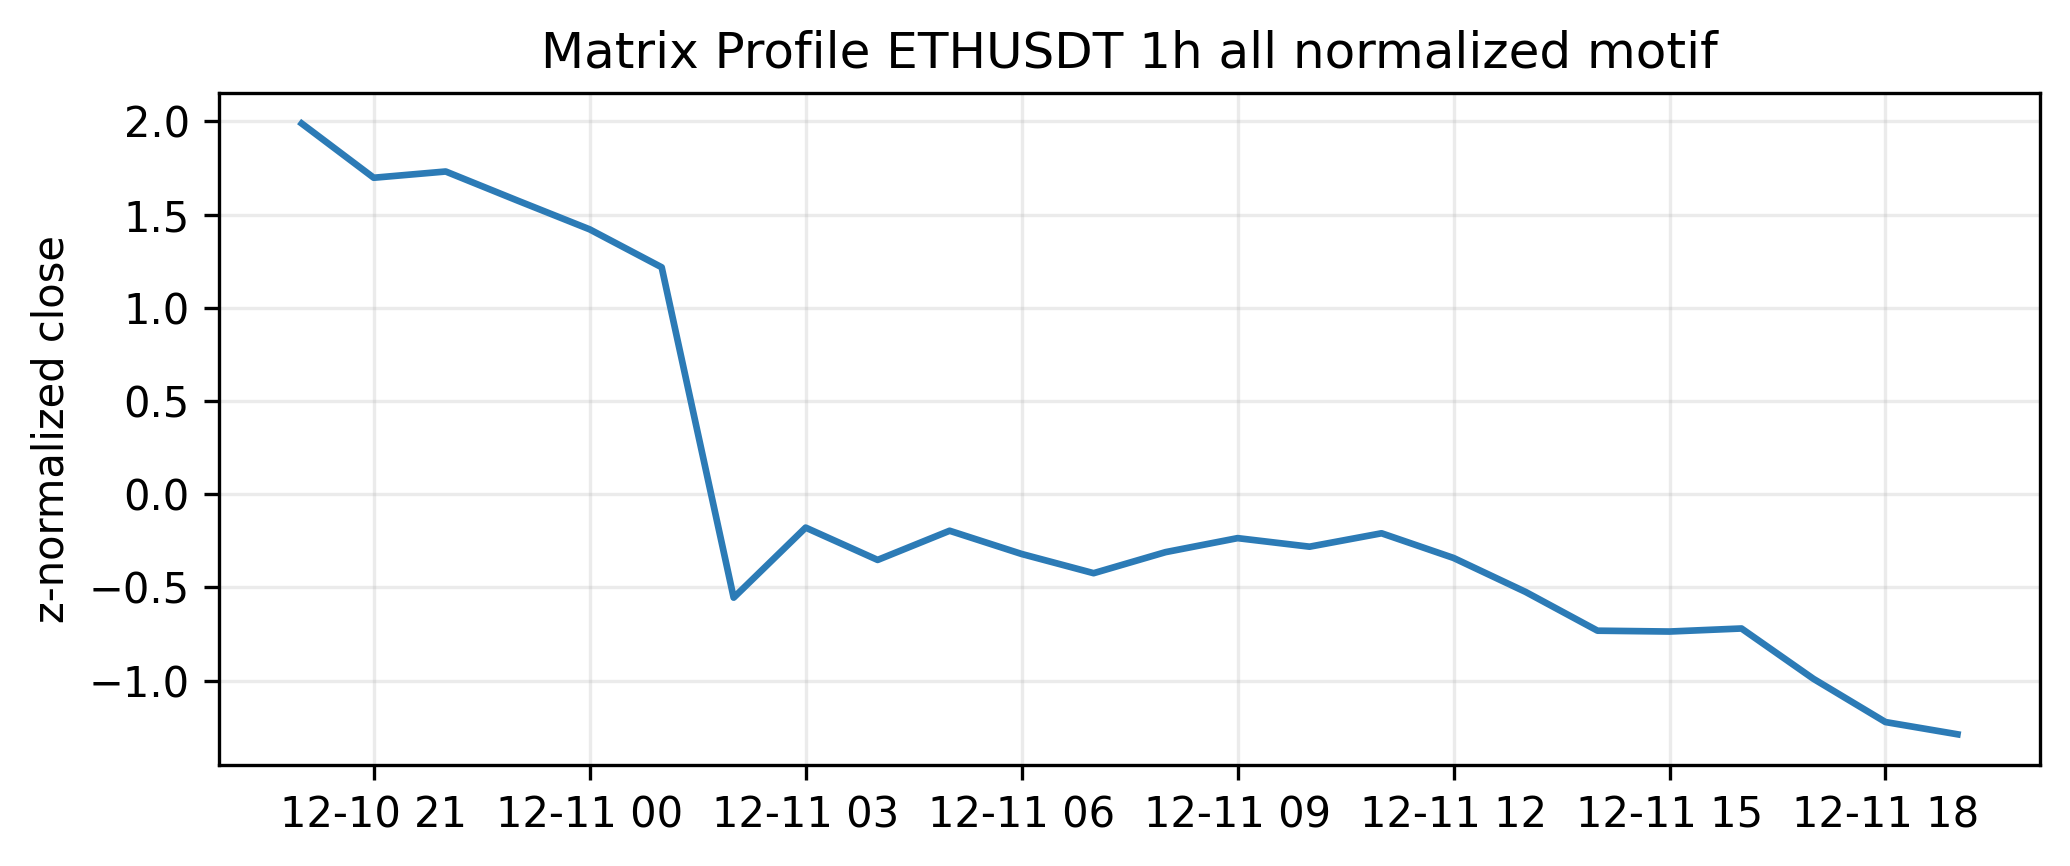
\includegraphics[width=0.9\linewidth]{reports/final_visual_evidence/figures/motif_30_matrix_profile_ethusdt_1h_all_1_0_pair27_2_normal_pattern.png}
\caption{motif 30 matrix profile ethusdt 1h all 1 0 pair27 2 normal pattern. The shaded interval marks the discovered motif occurrence in original price context.}
\end{figure}

\begin{figure}[ht]
\centering
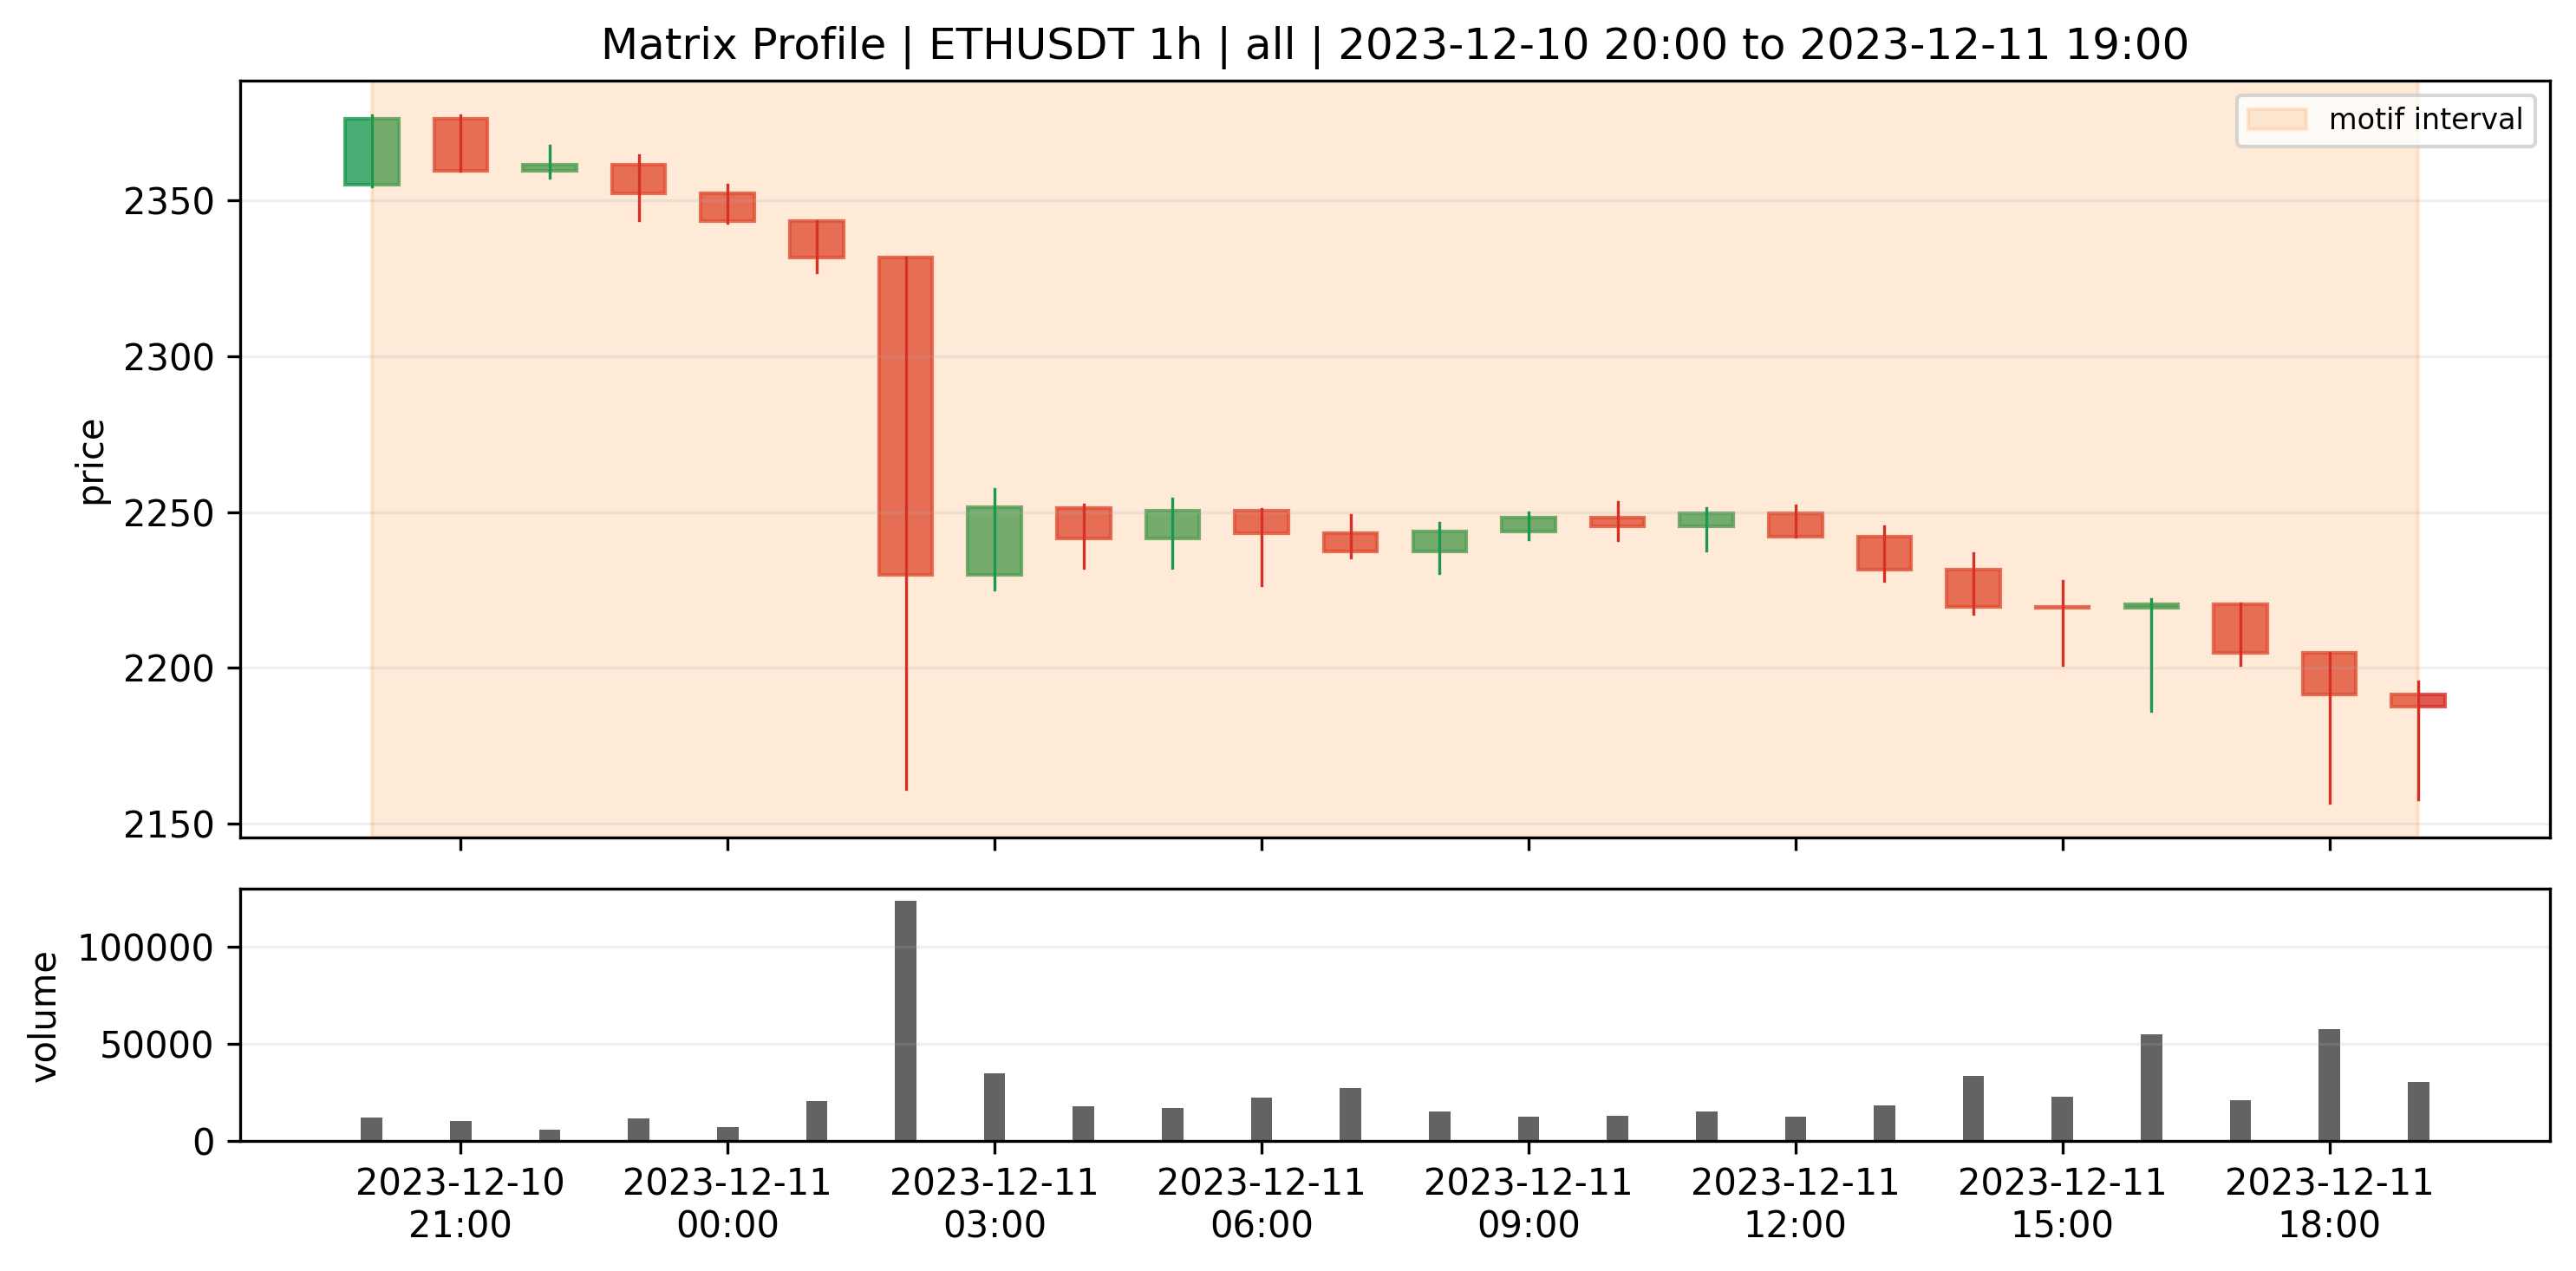
\includegraphics[width=0.9\linewidth]{reports/final_visual_evidence/figures/motif_30_matrix_profile_ethusdt_1h_all_1_0_pair27_2_zoom.png}
\caption{motif 30 matrix profile ethusdt 1h all 1 0 pair27 2 zoom. The shaded interval marks the discovered motif occurrence in original price context.}
\end{figure}

\begin{figure}[ht]
\centering
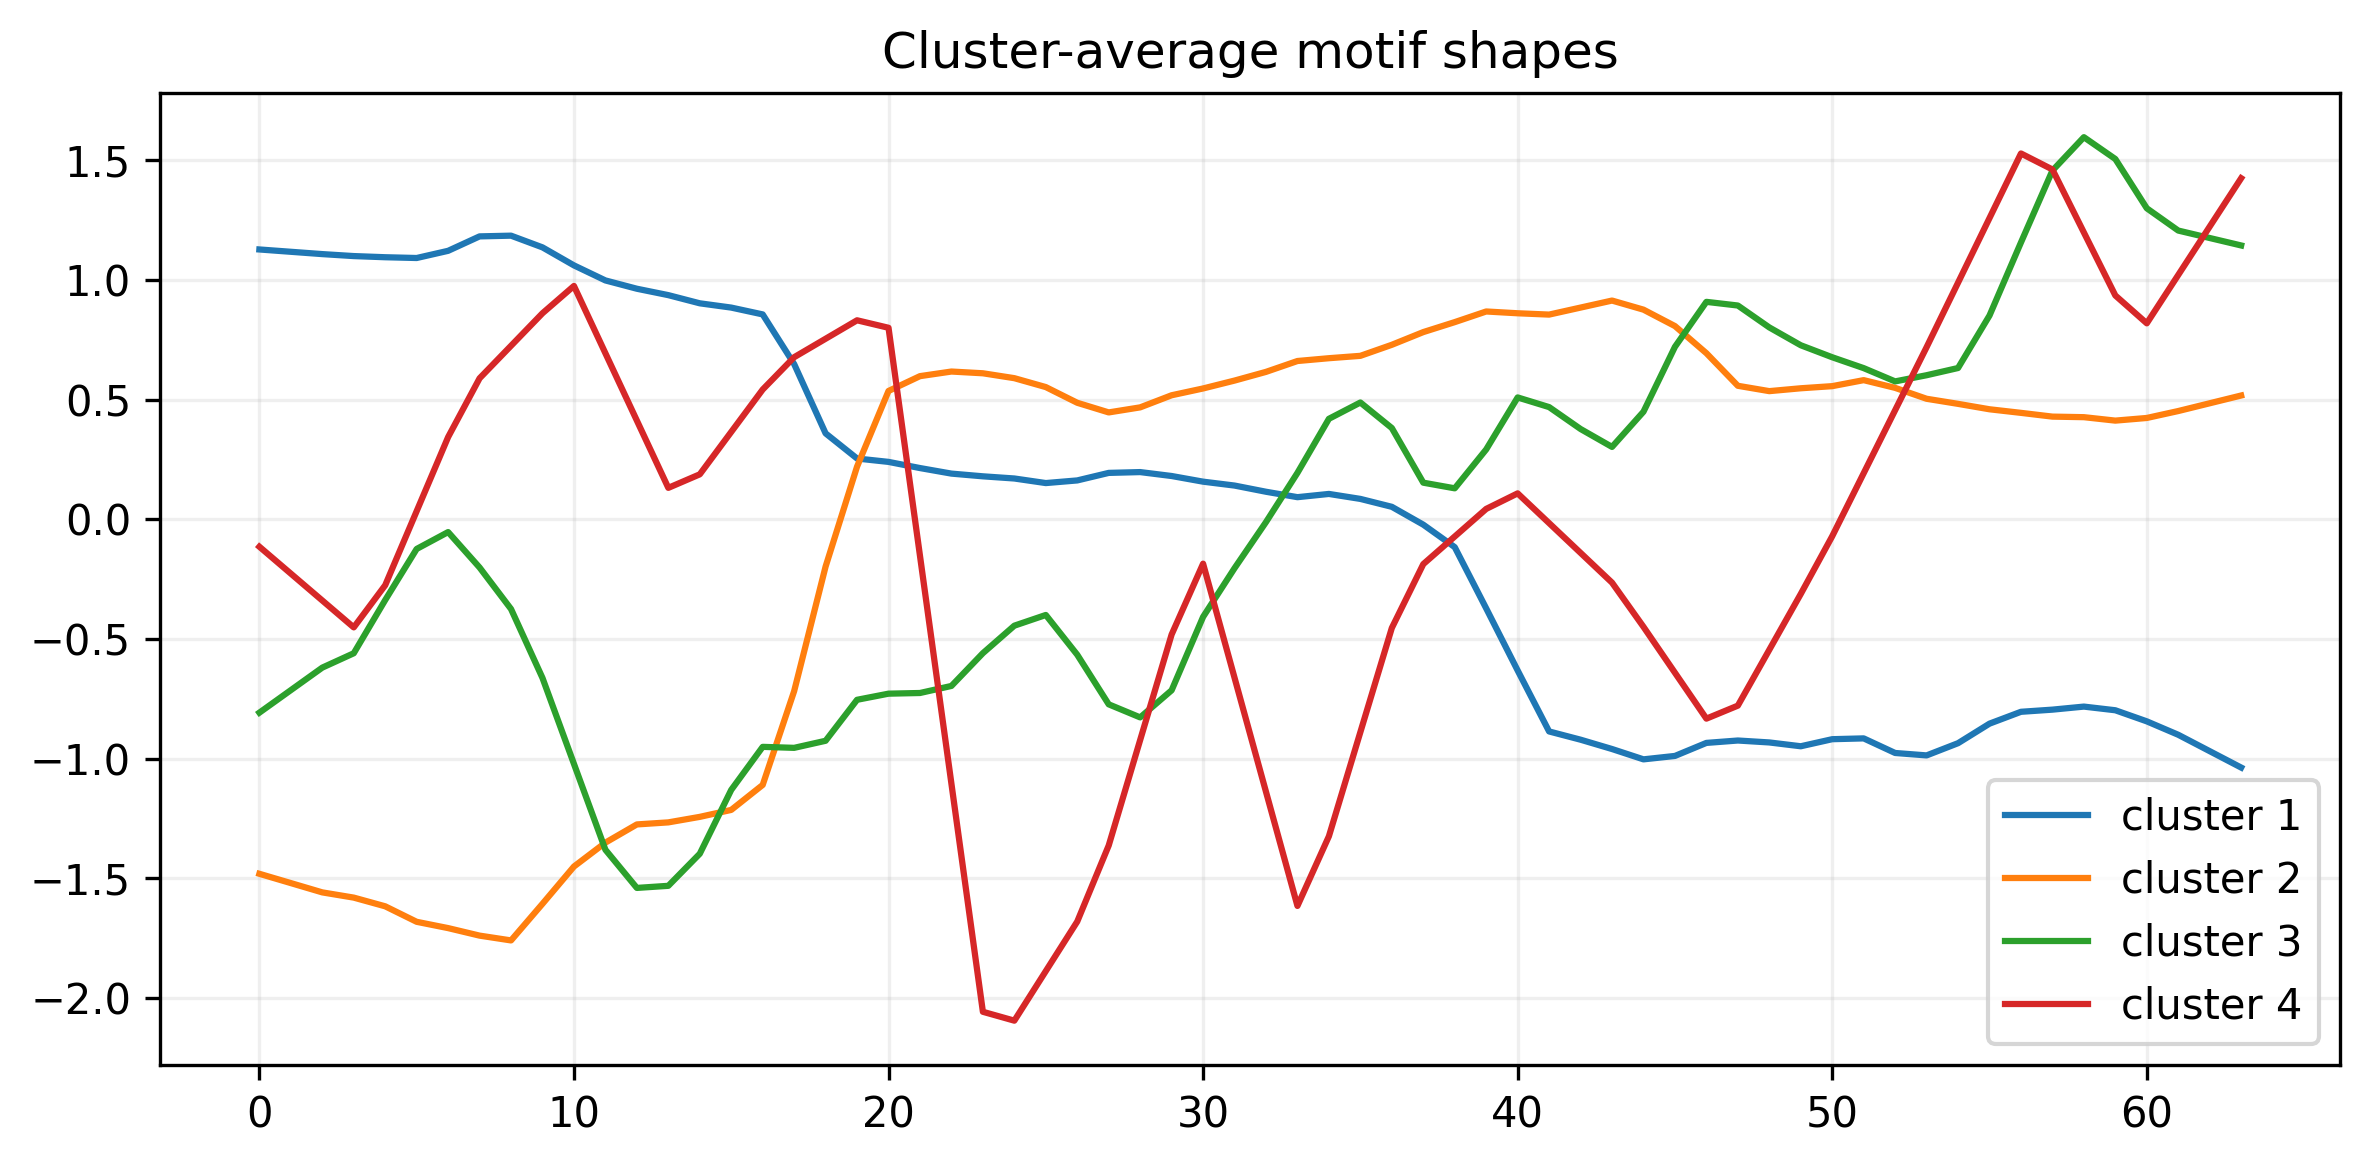
\includegraphics[width=0.9\linewidth]{reports/final_visual_evidence/figures/motif_cluster_average_shapes.png}
\caption{motif cluster average shapes. The shaded interval marks the discovered motif occurrence in original price context.}
\end{figure}

\begin{figure}[ht]
\centering
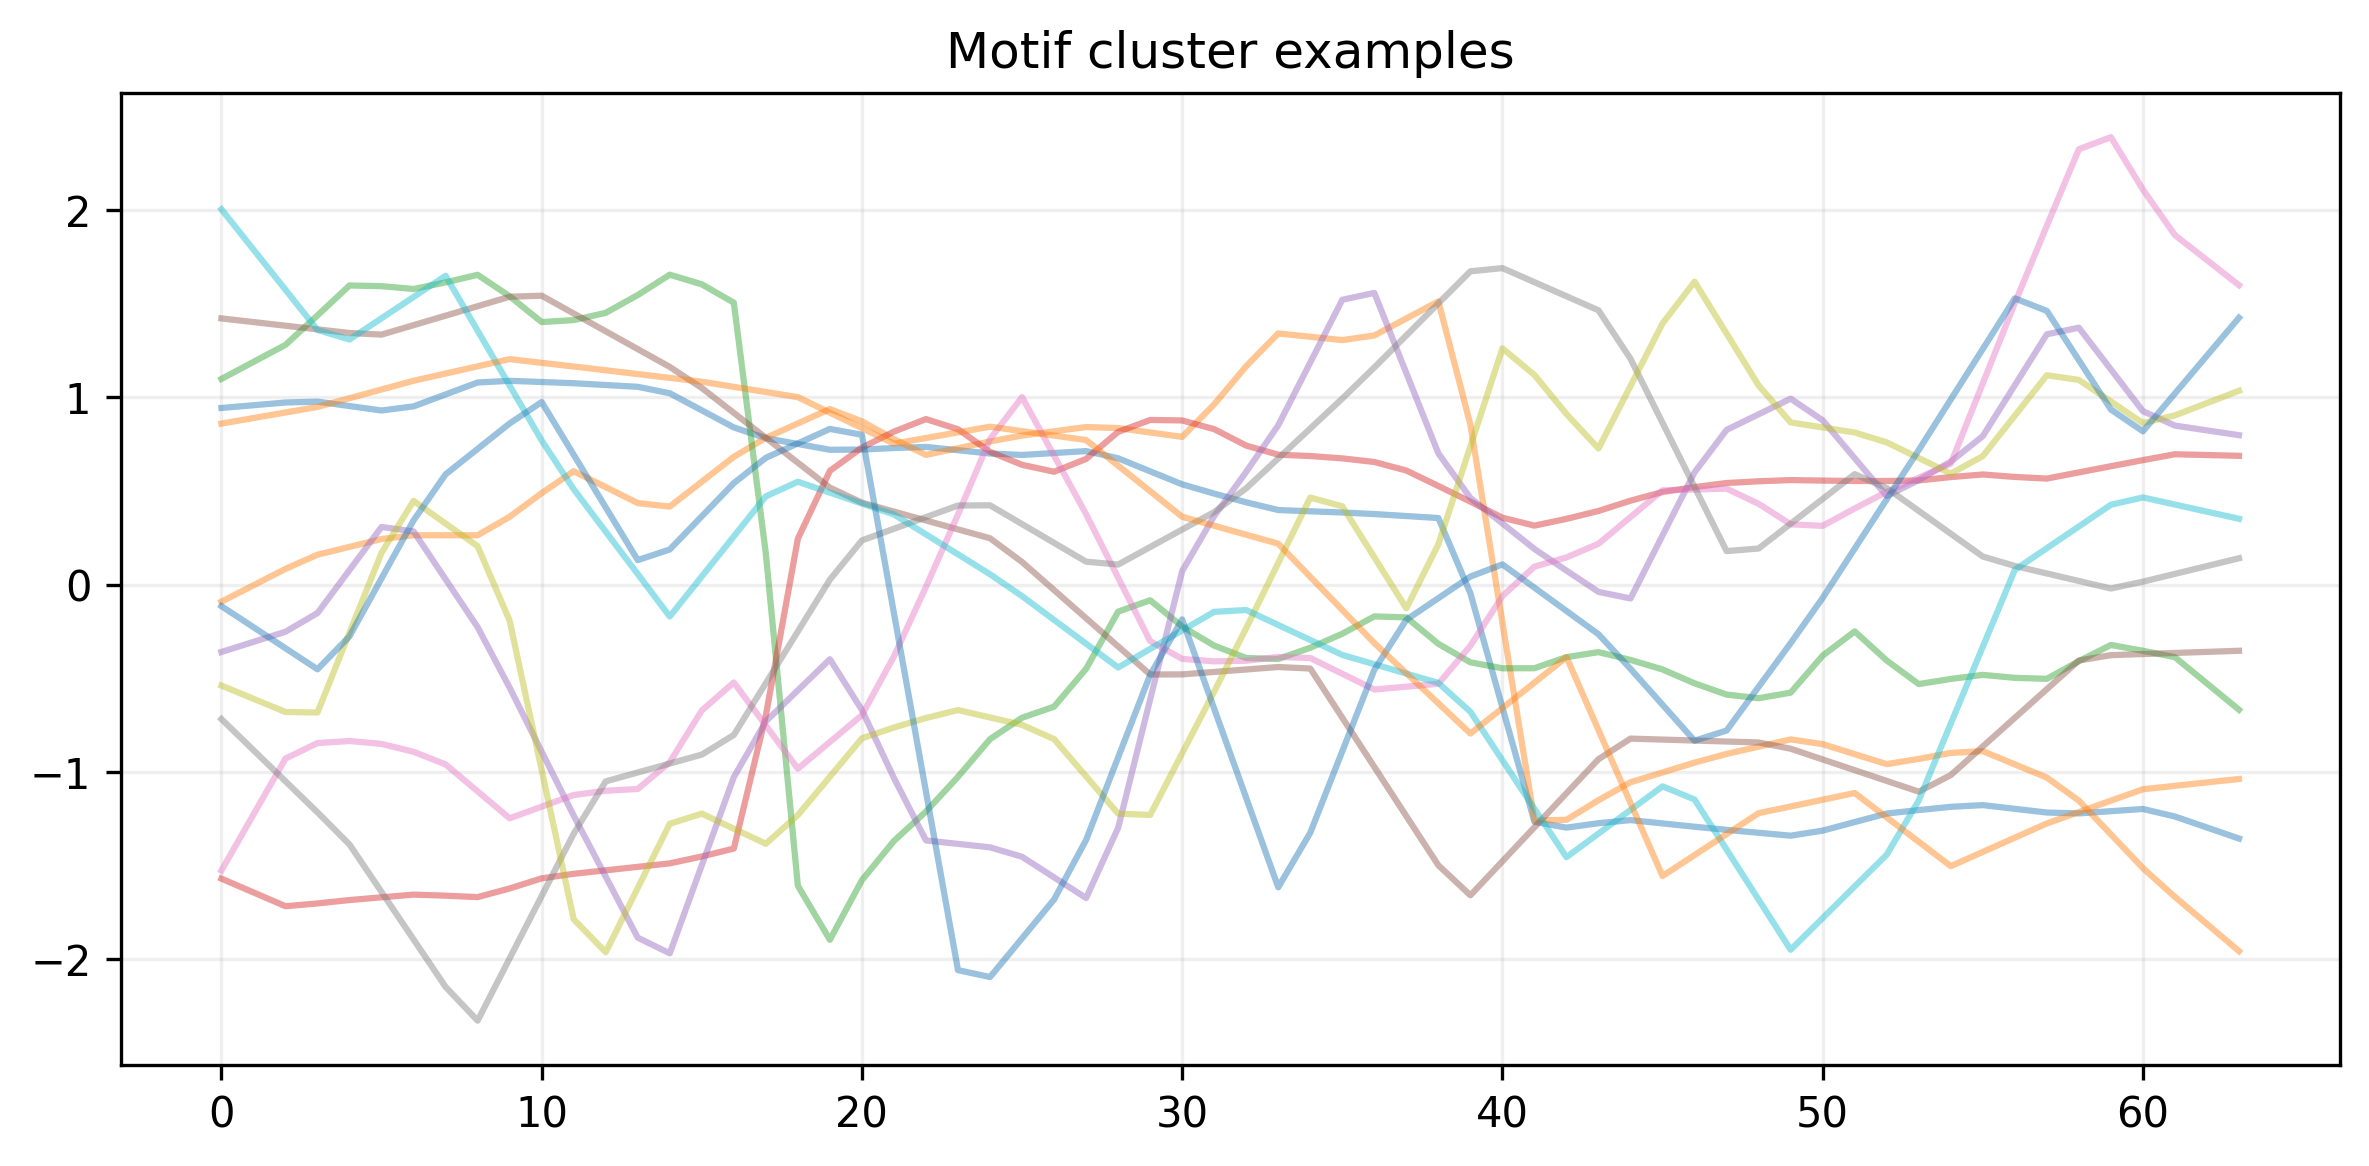
\includegraphics[width=0.9\linewidth]{reports/final_visual_evidence/figures/motif_cluster_examples.png}
\caption{motif cluster examples. The shaded interval marks the discovered motif occurrence in original price context.}
\end{figure}

\begin{figure}[ht]
\centering
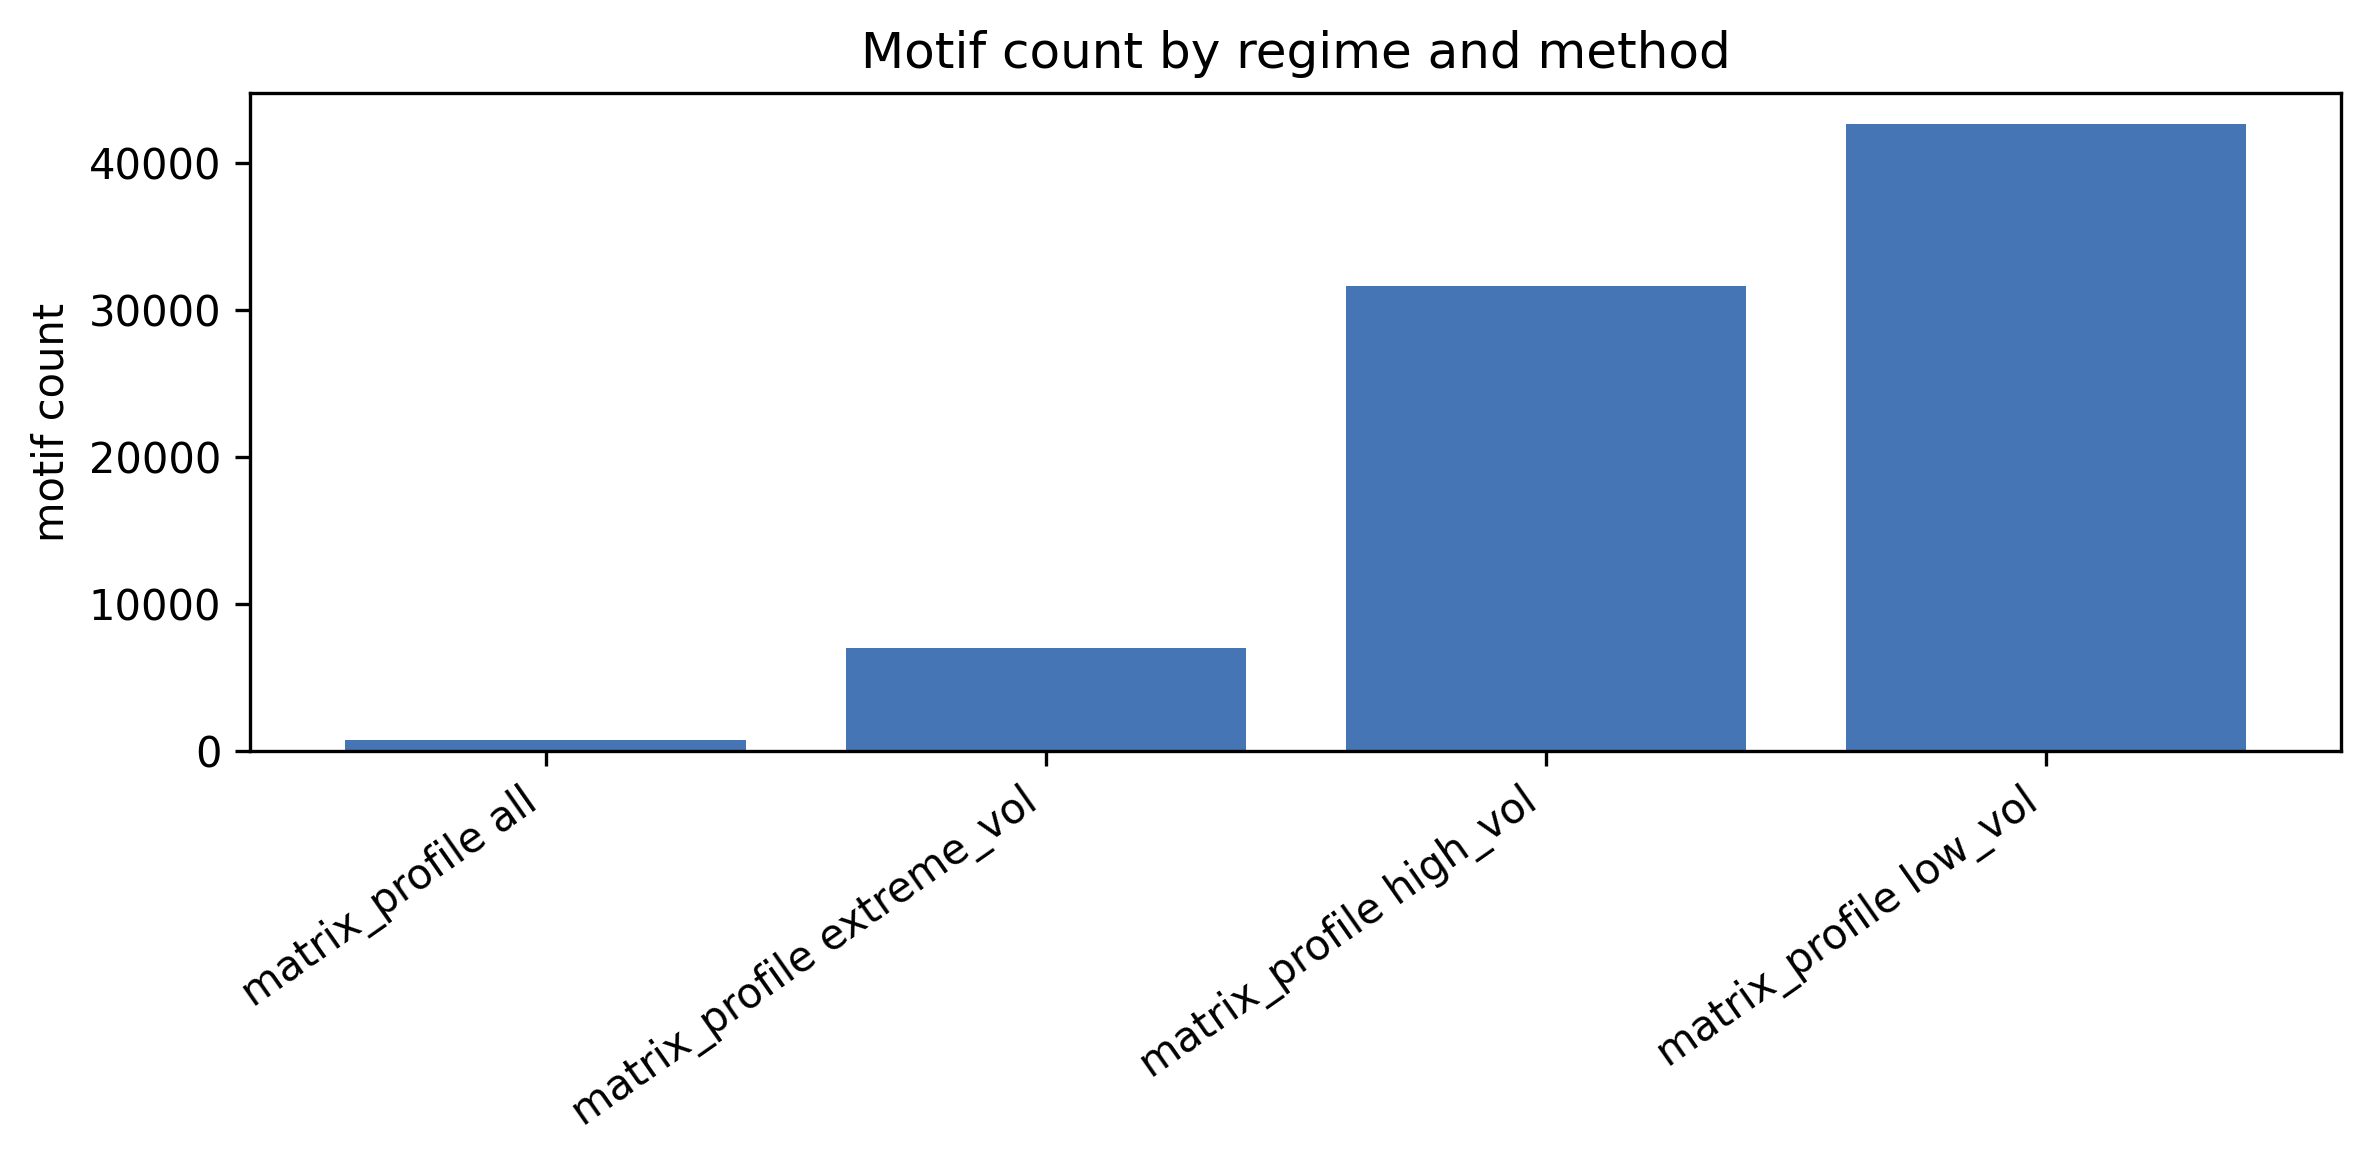
\includegraphics[width=0.9\linewidth]{reports/final_visual_evidence/figures/motif_count_by_regime_and_method.png}
\caption{motif count by regime and method. The shaded interval marks the discovered motif occurrence in original price context.}
\end{figure}

\begin{figure}[ht]
\centering
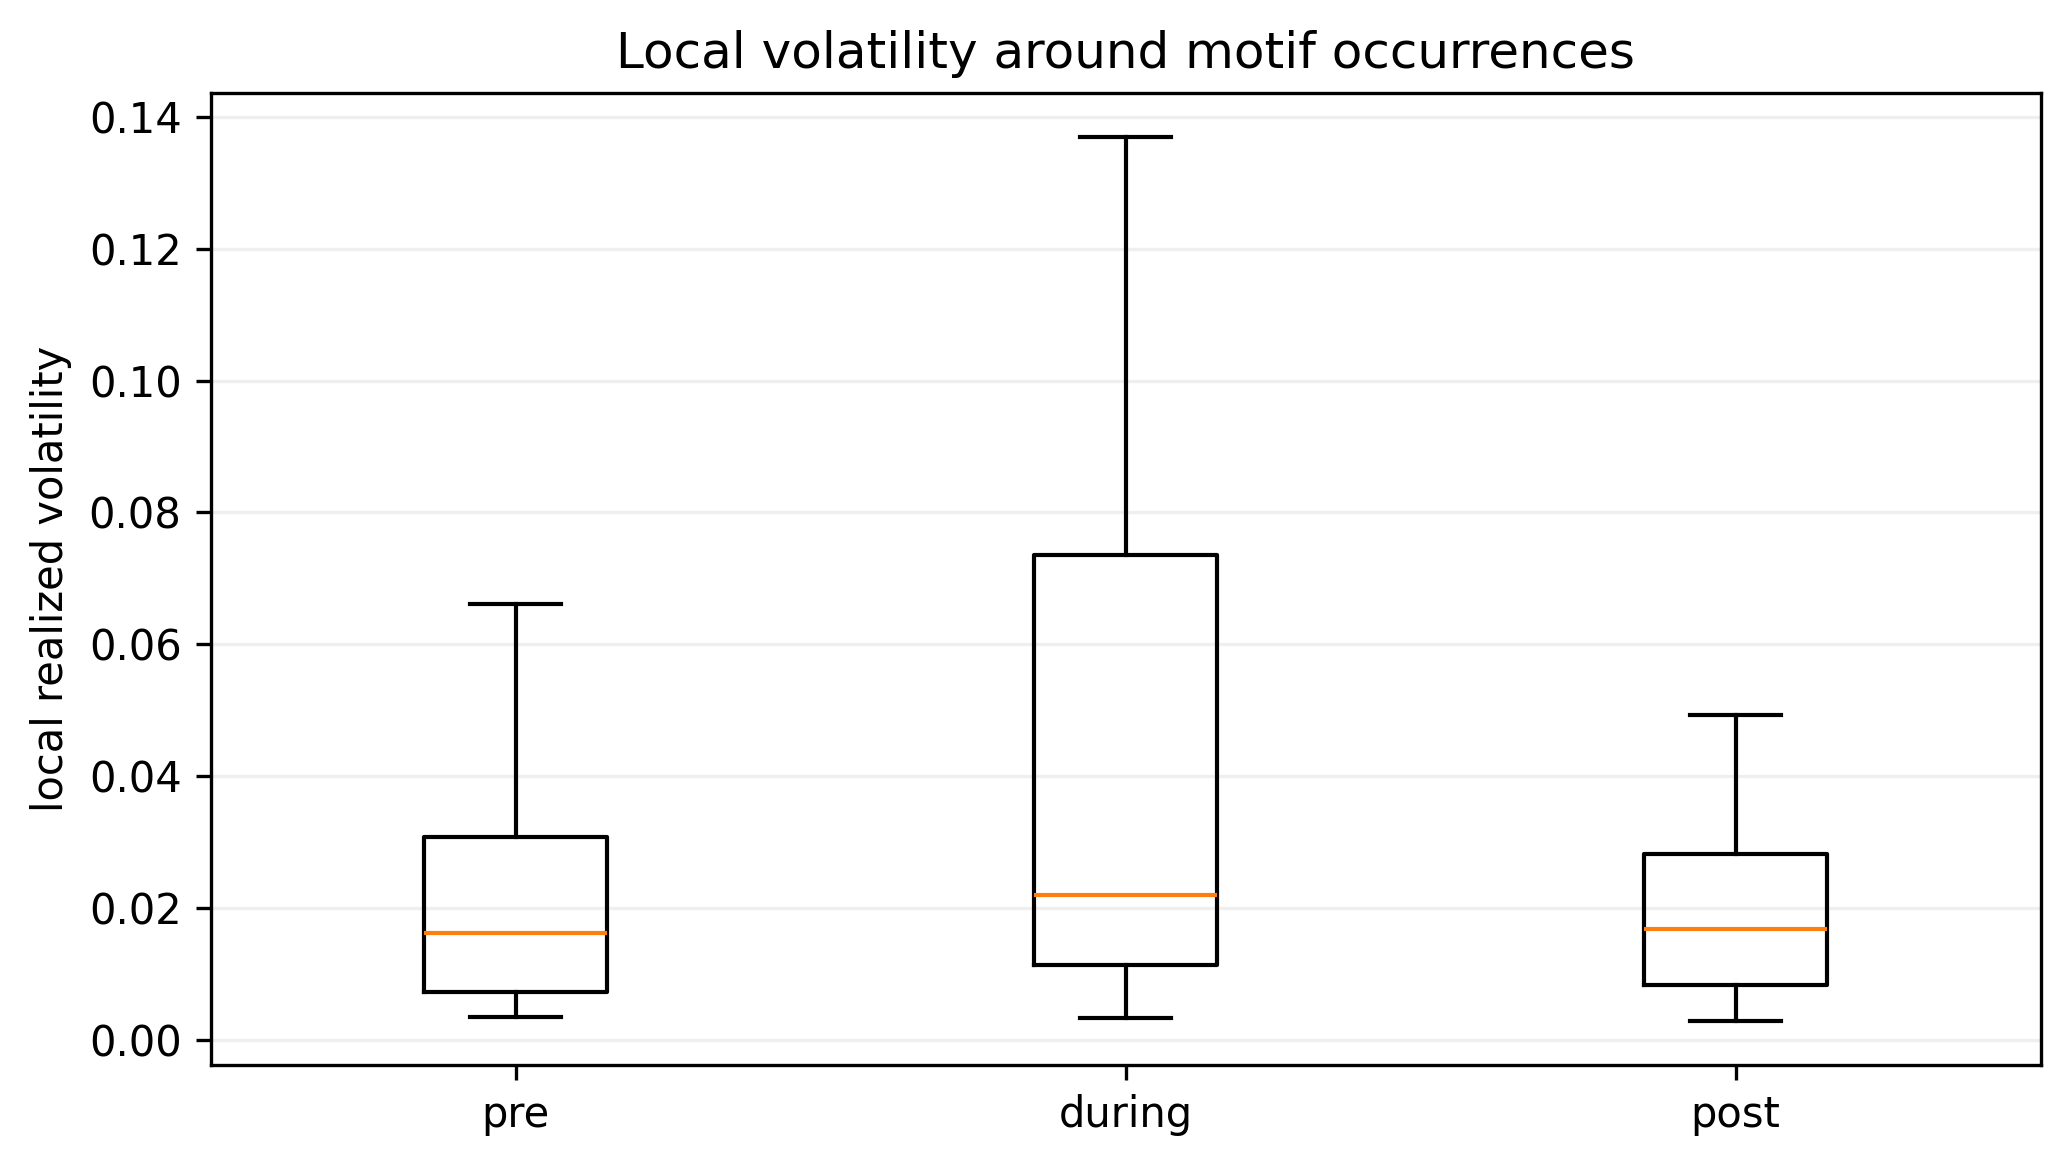
\includegraphics[width=0.9\linewidth]{reports/final_visual_evidence/figures/motif_local_volatility_pre_during_post.png}
\caption{motif local volatility pre during post. The shaded interval marks the discovered motif occurrence in original price context.}
\end{figure}

\begin{figure}[ht]
\centering
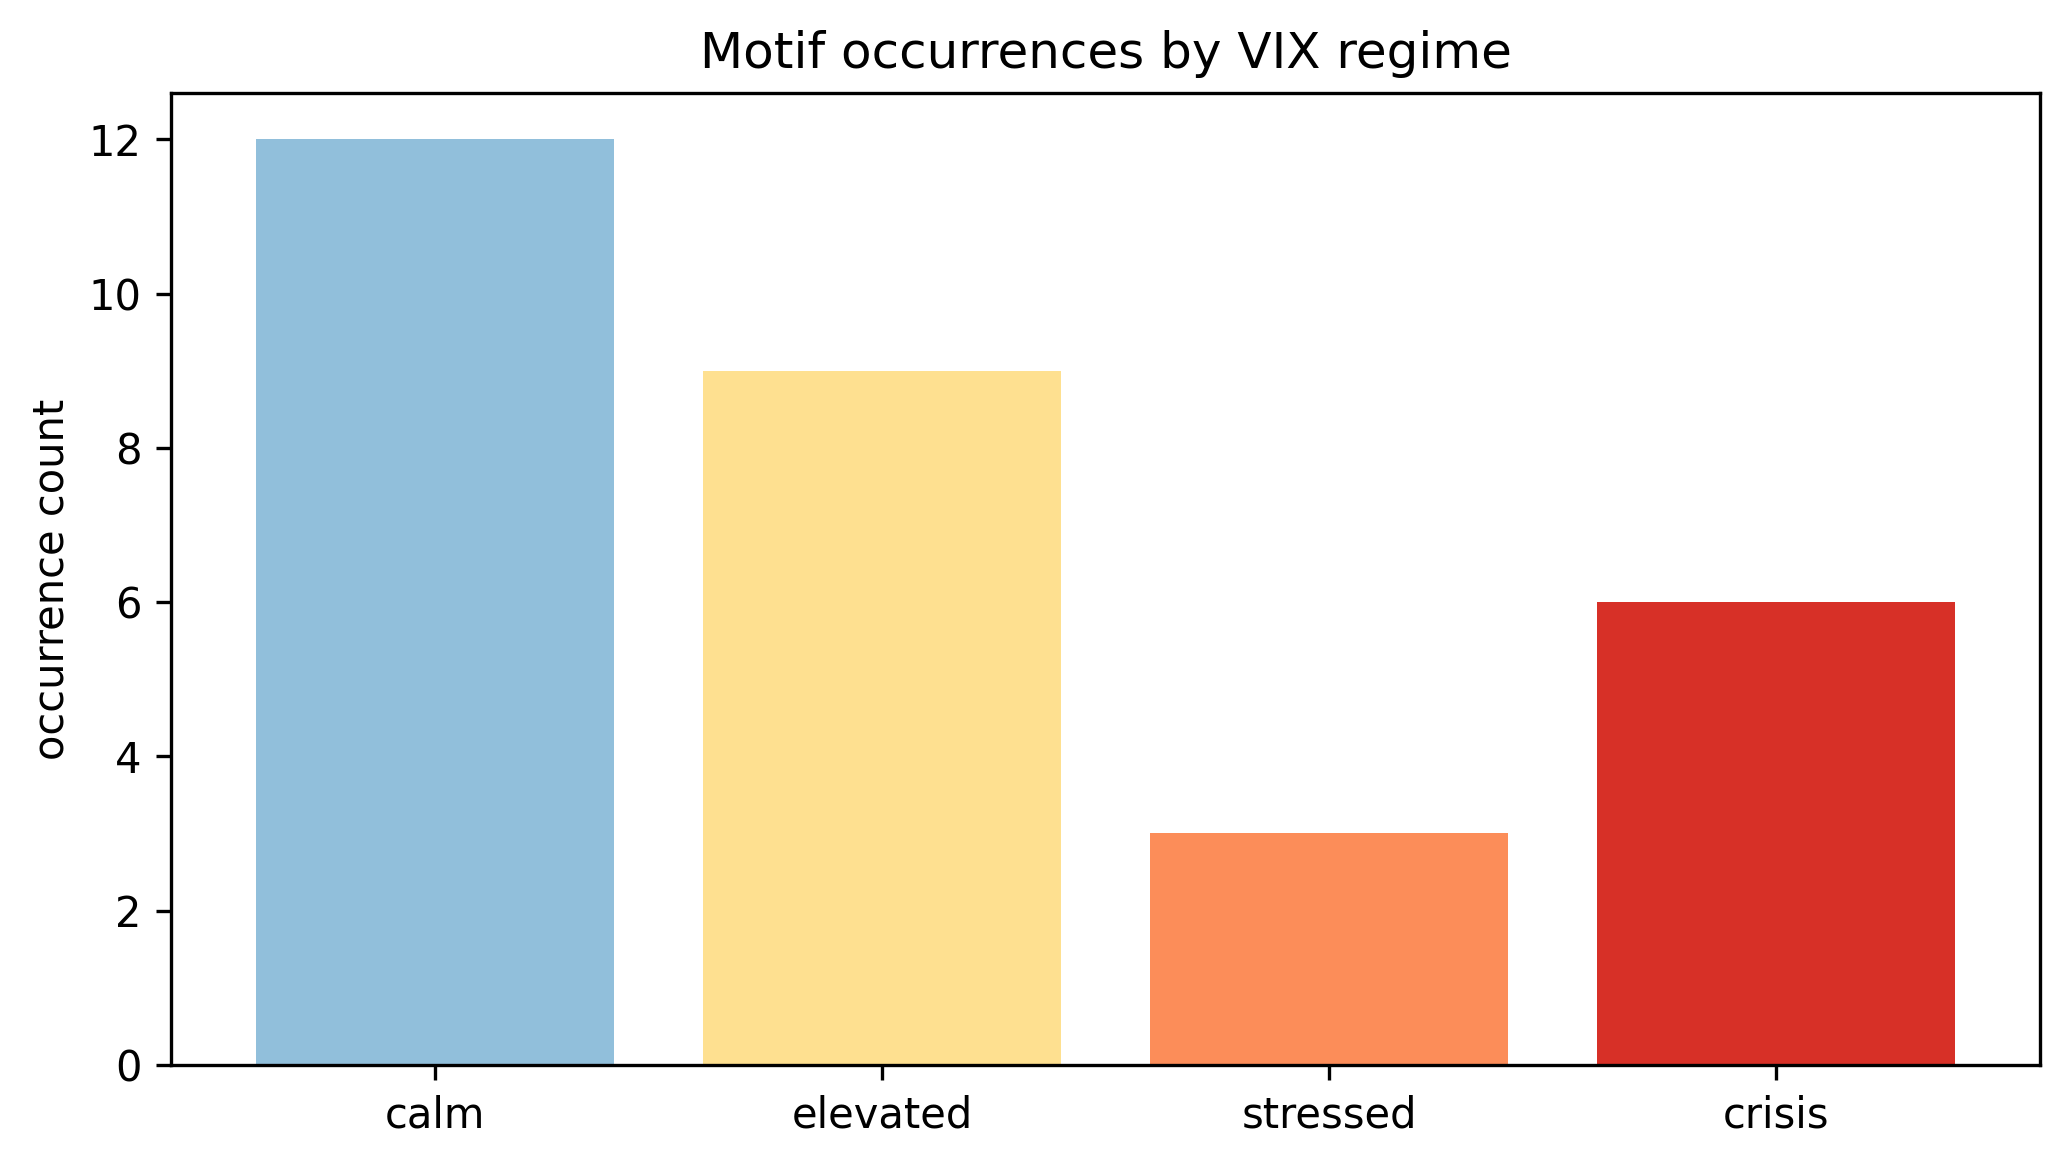
\includegraphics[width=0.9\linewidth]{reports/final_visual_evidence/figures/motif_occurrences_by_vix_regime.png}
\caption{motif occurrences by vix regime. VIX is external market-stress context only and is not used as a motif-discovery label.}
\end{figure}

\begin{figure}[ht]
\centering
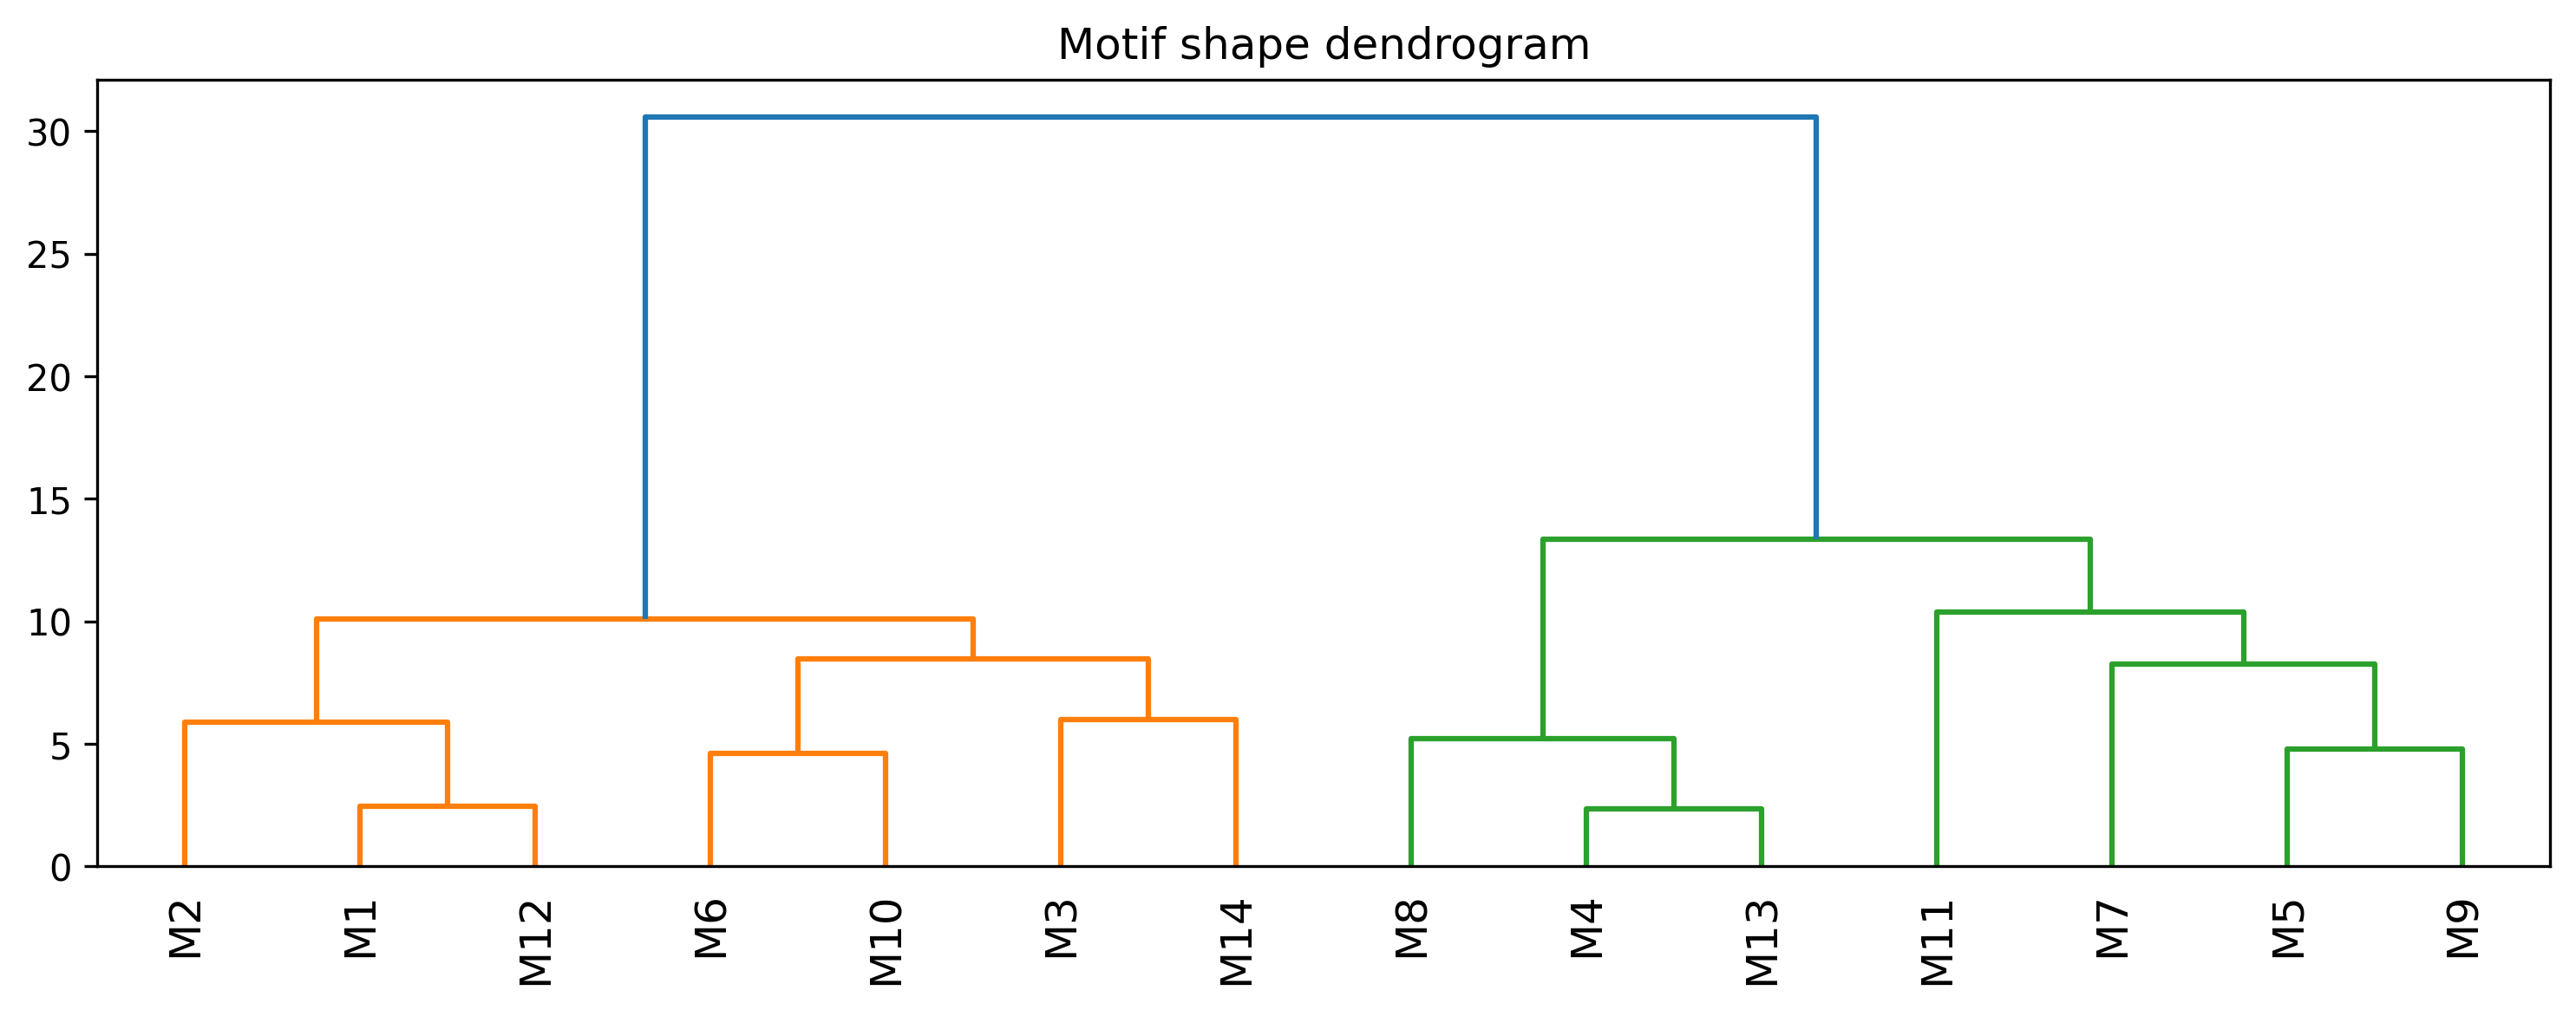
\includegraphics[width=0.9\linewidth]{reports/final_visual_evidence/figures/motif_shape_dendrogram.png}
\caption{motif shape dendrogram. The shaded interval marks the discovered motif occurrence in original price context.}
\end{figure}

\begin{figure}[ht]
\centering
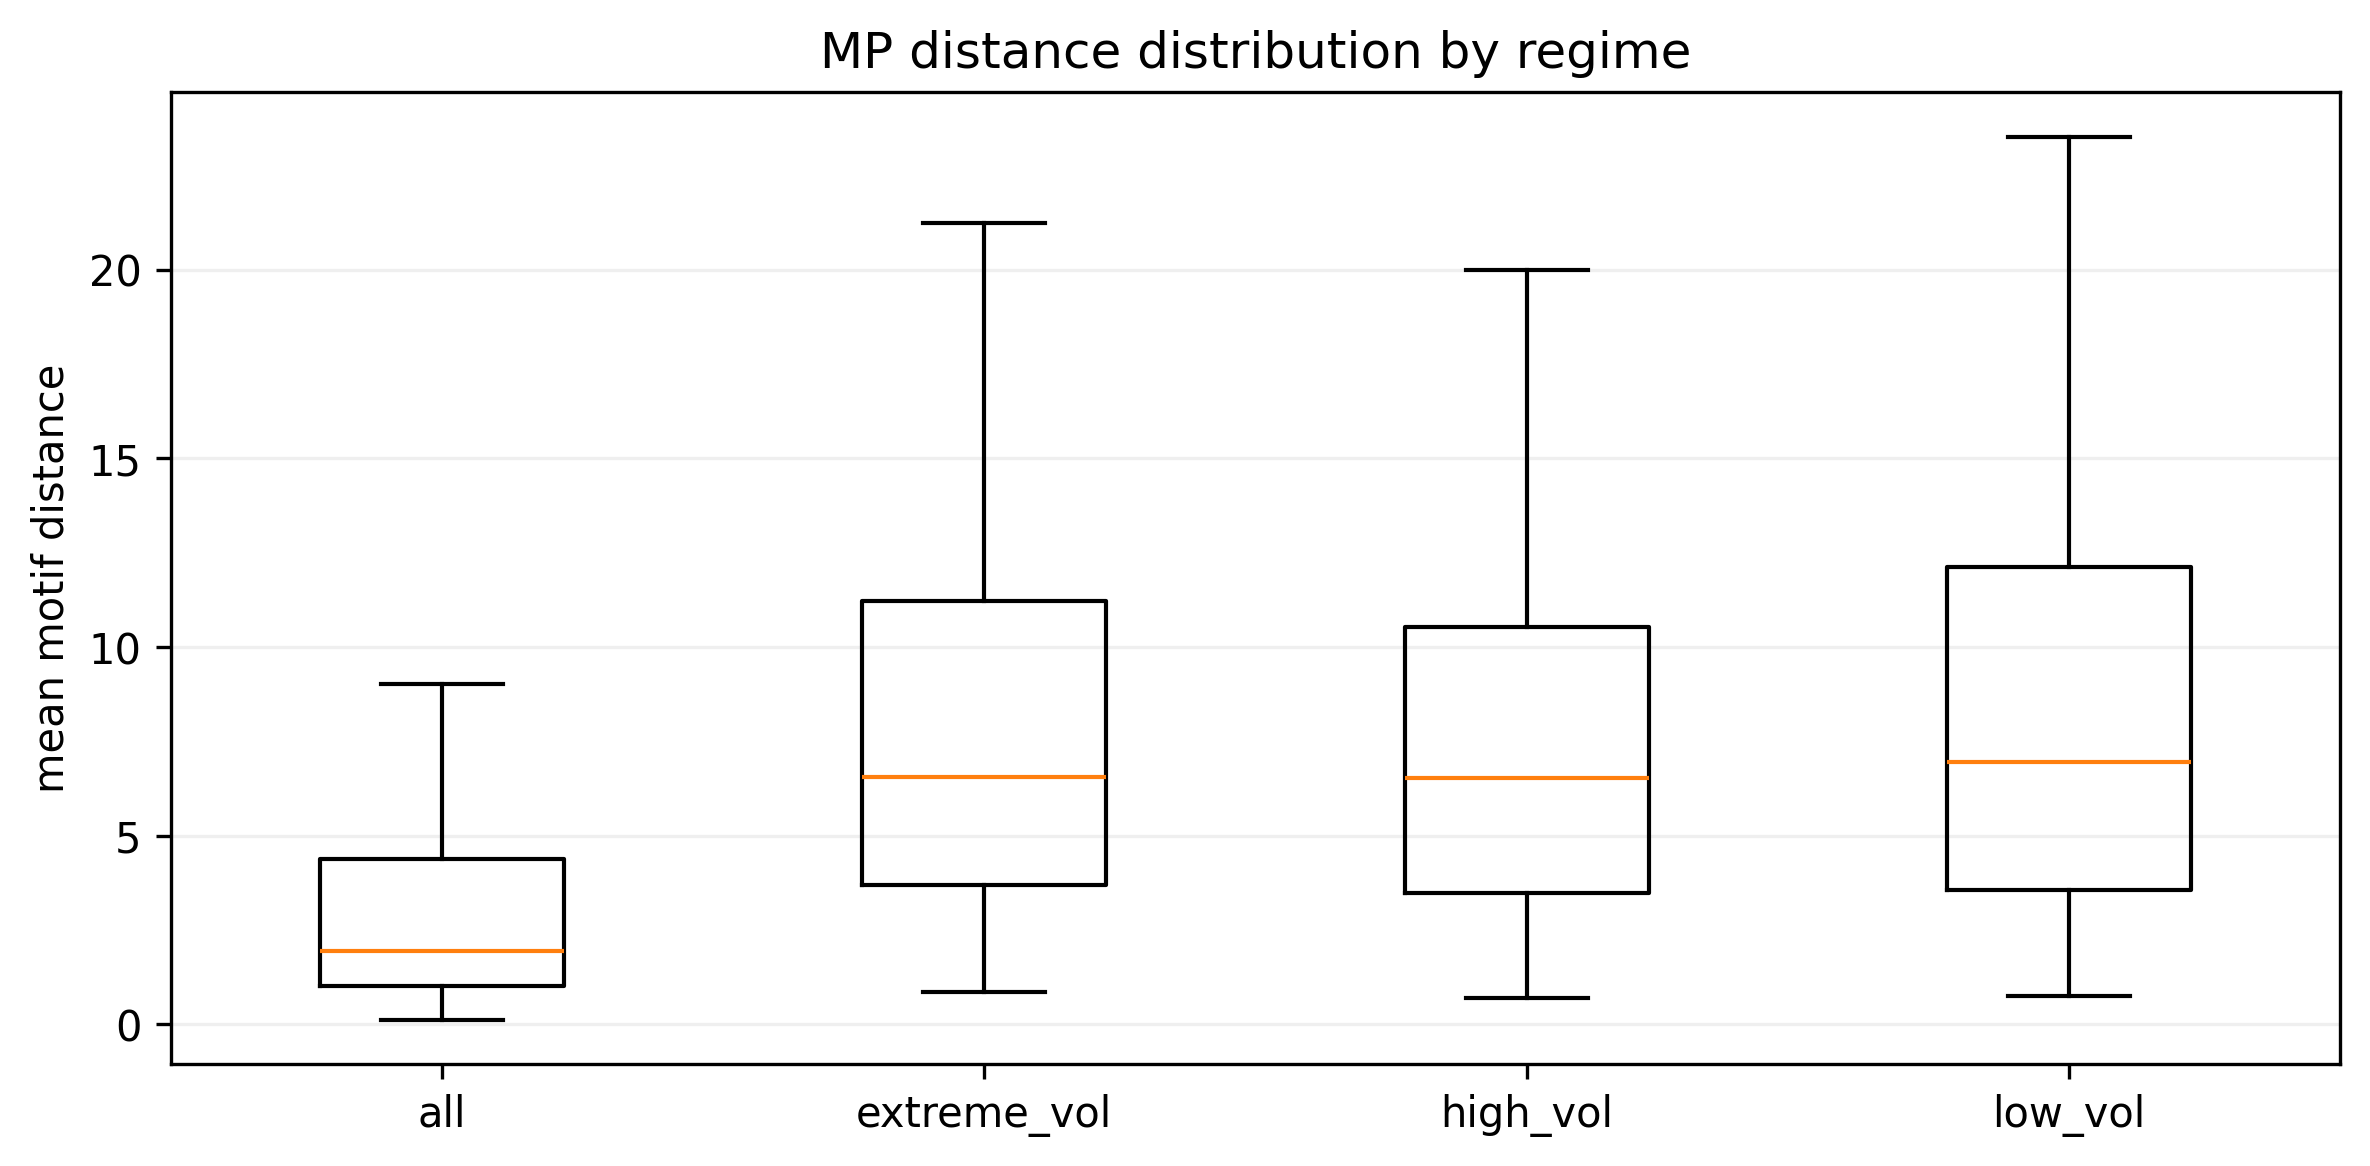
\includegraphics[width=0.9\linewidth]{reports/final_visual_evidence/figures/mp_distance_distribution_by_regime.png}
\caption{mp distance distribution by regime.}
\end{figure}

\begin{figure}[ht]
\centering
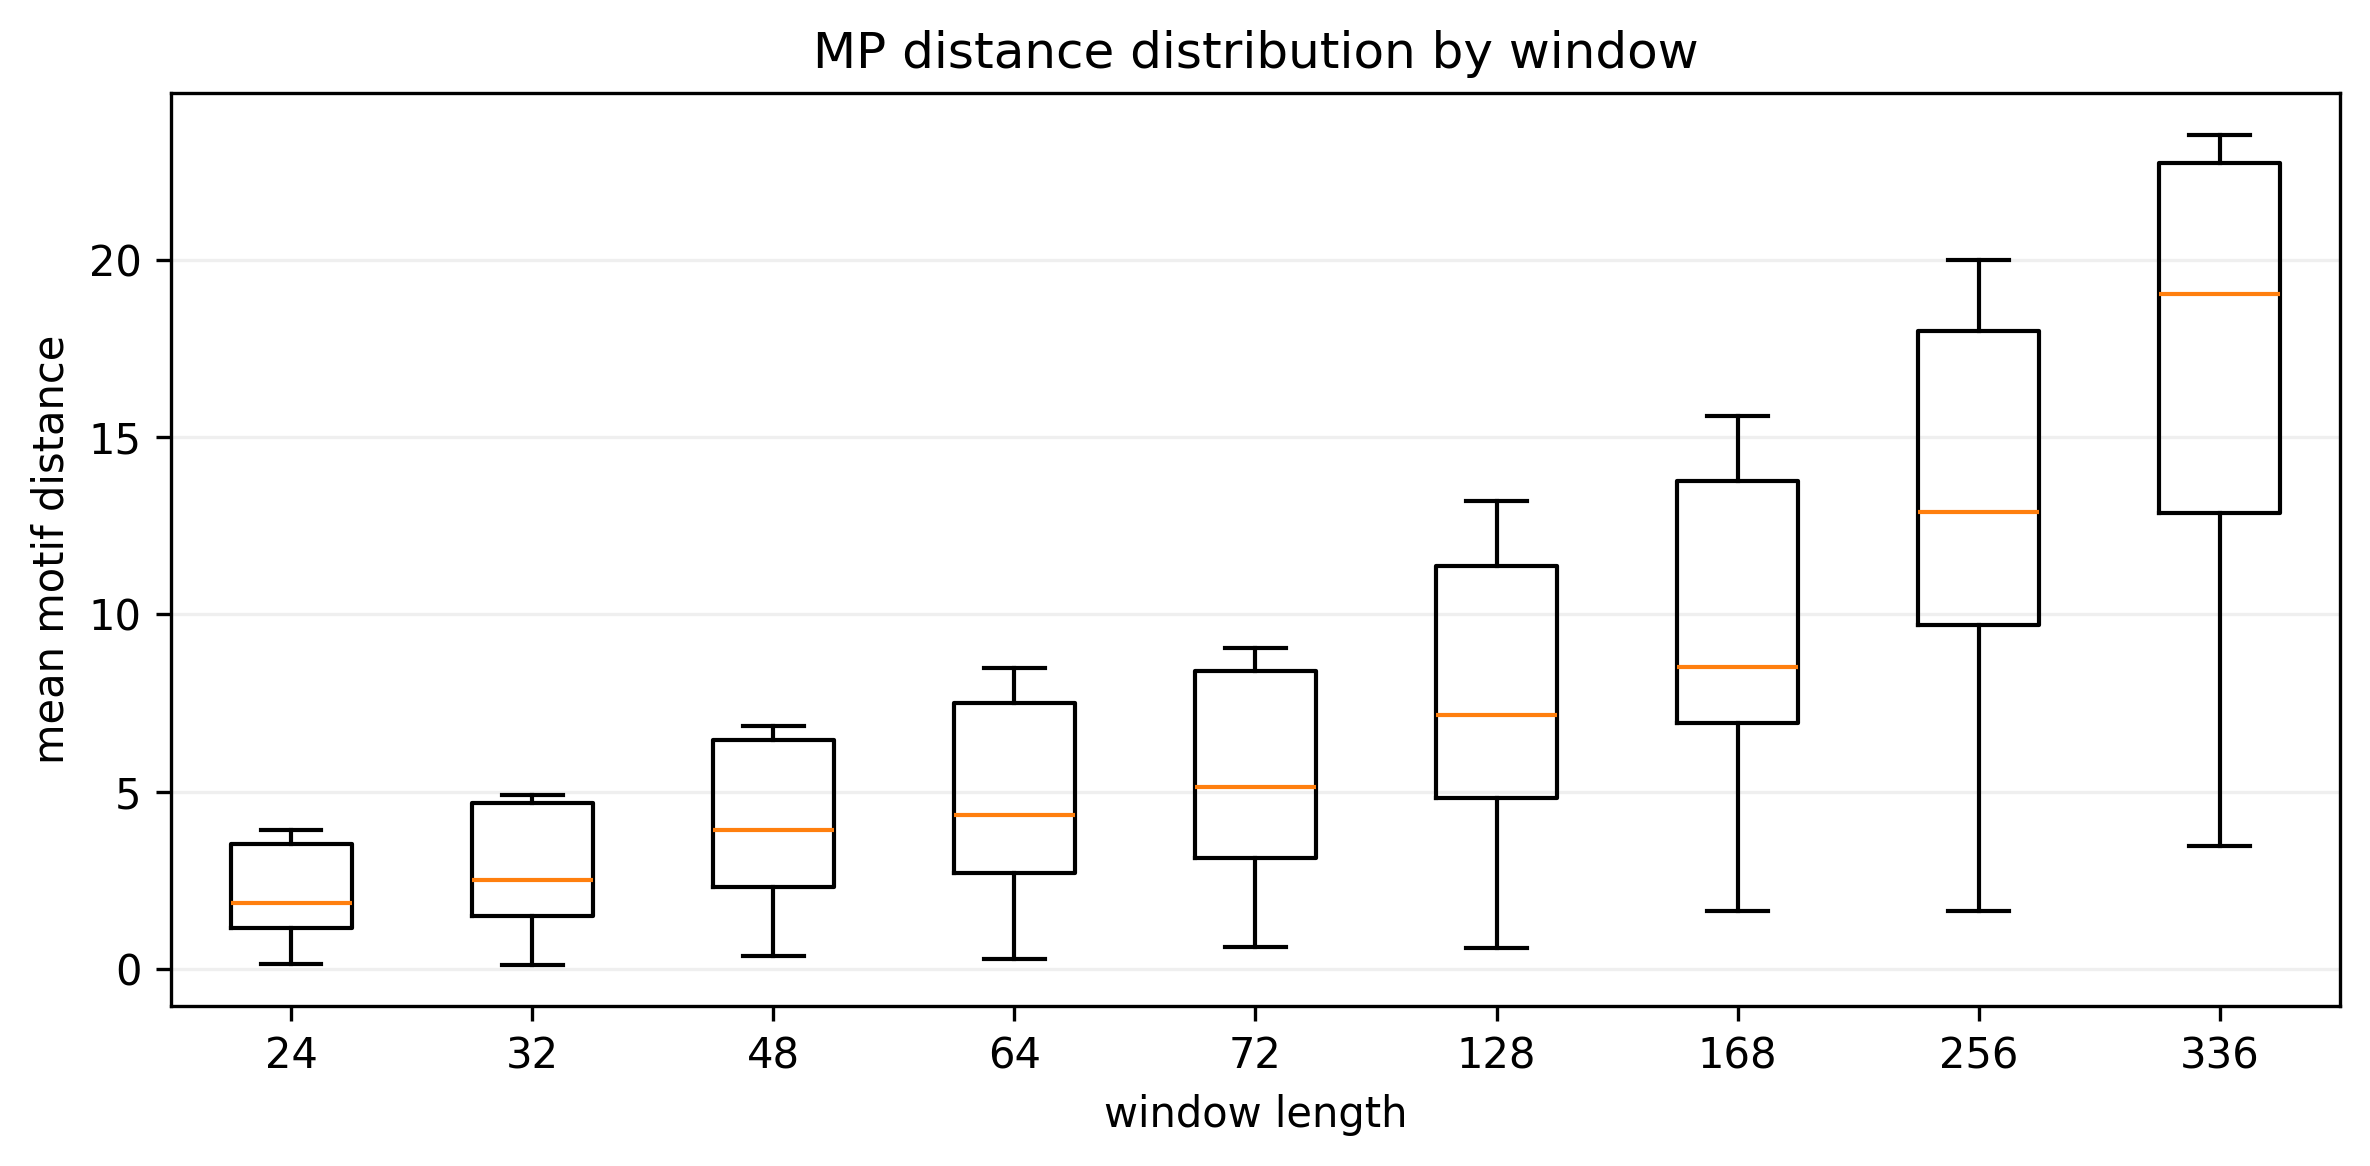
\includegraphics[width=0.9\linewidth]{reports/final_visual_evidence/figures/mp_distance_distribution_by_window.png}
\caption{mp distance distribution by window.}
\end{figure}

\begin{figure}[ht]
\centering
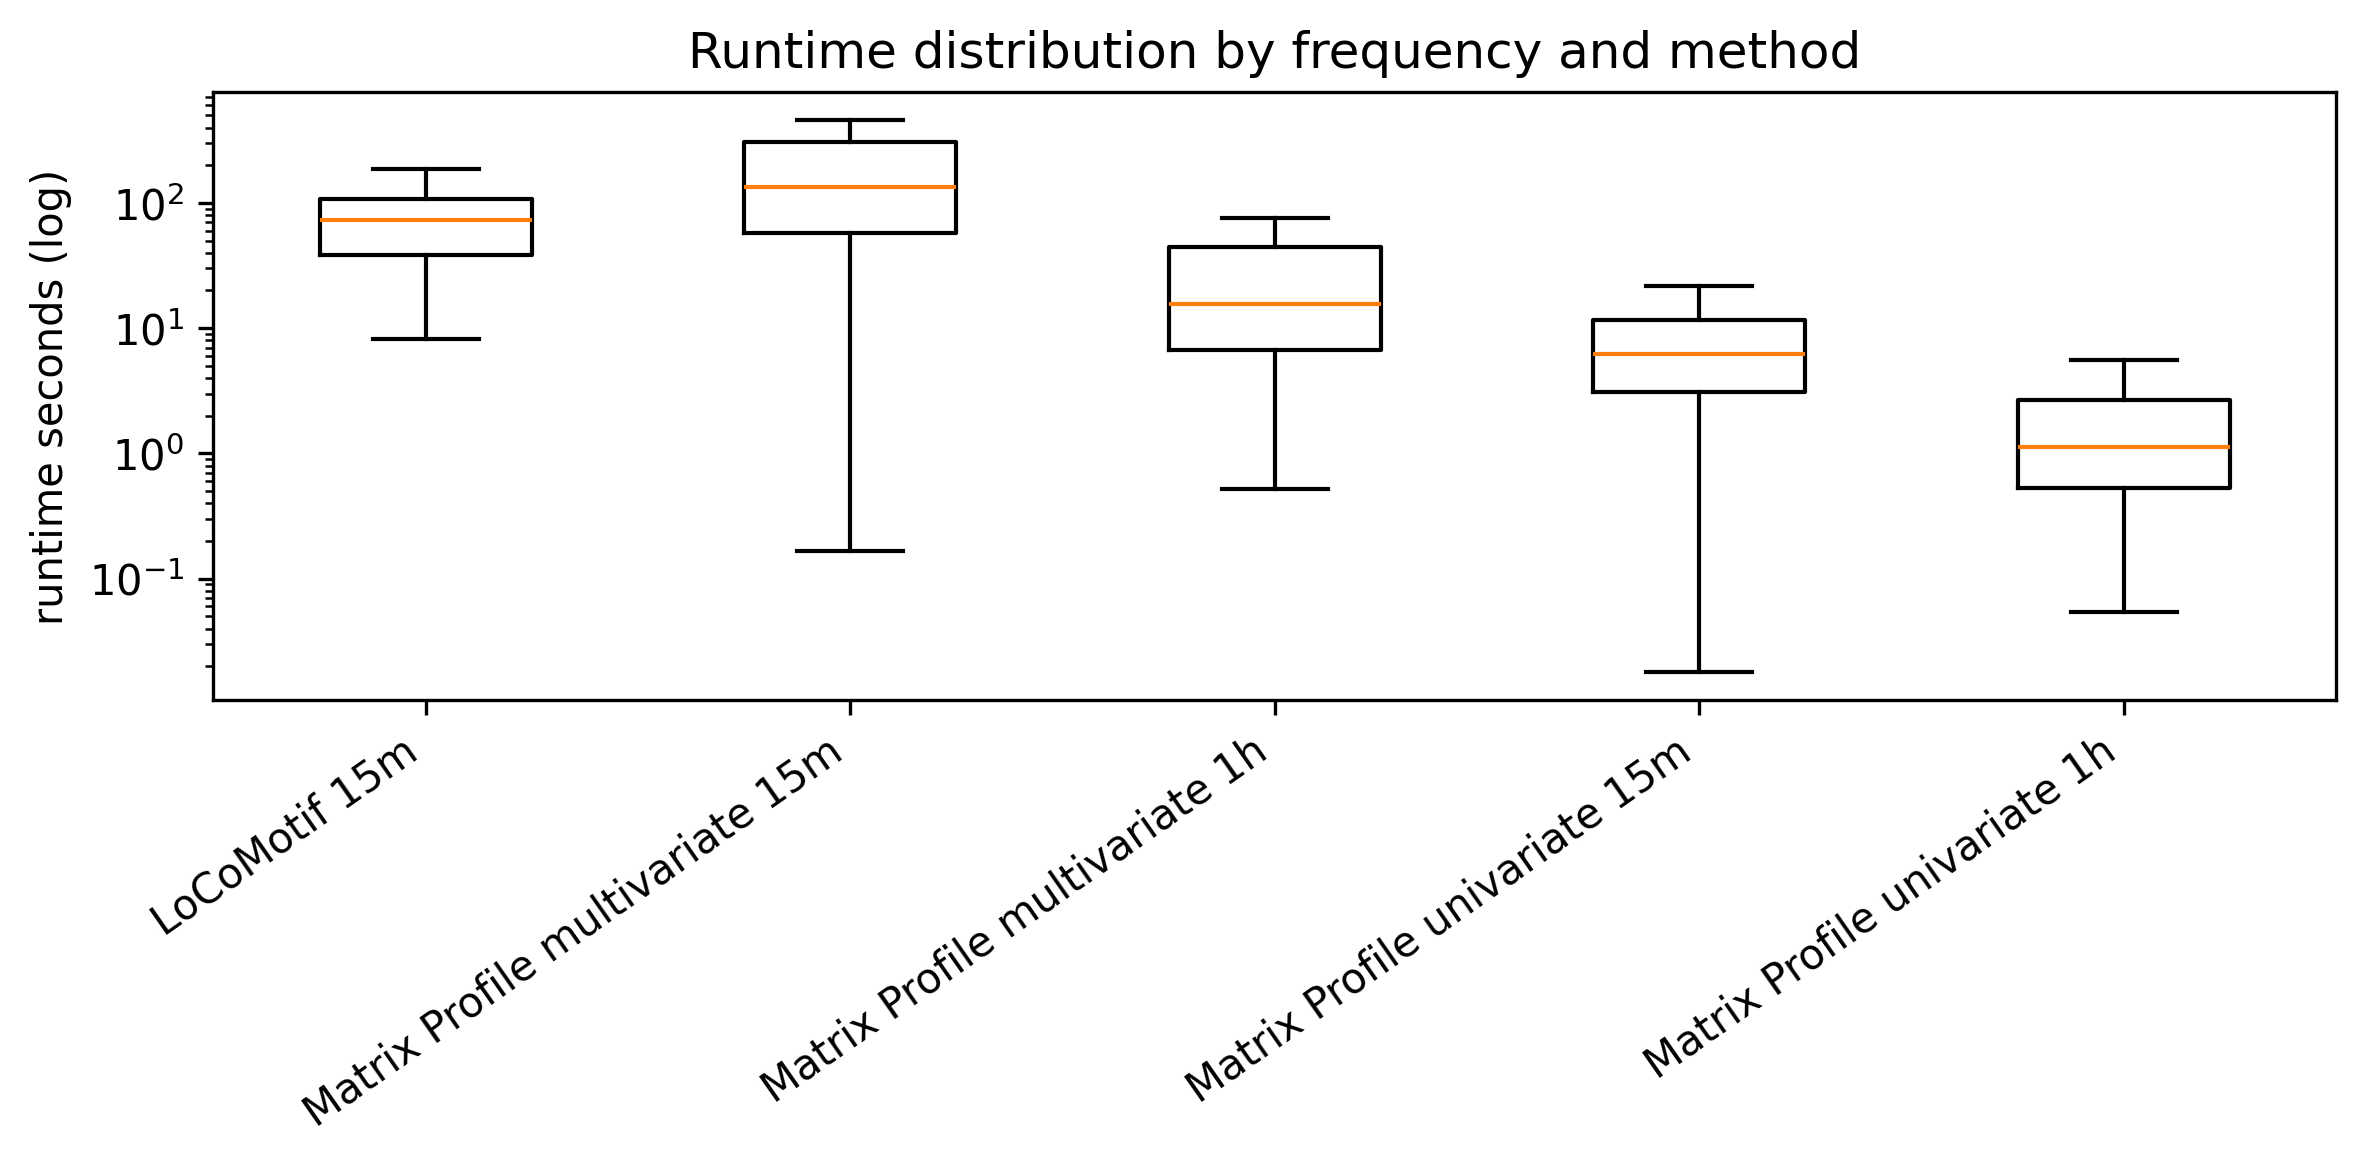
\includegraphics[width=0.9\linewidth]{reports/final_visual_evidence/figures/mp_runtime_distribution_by_frequency.png}
\caption{mp runtime distribution by frequency.}
\end{figure}

\begin{figure}[ht]
\centering
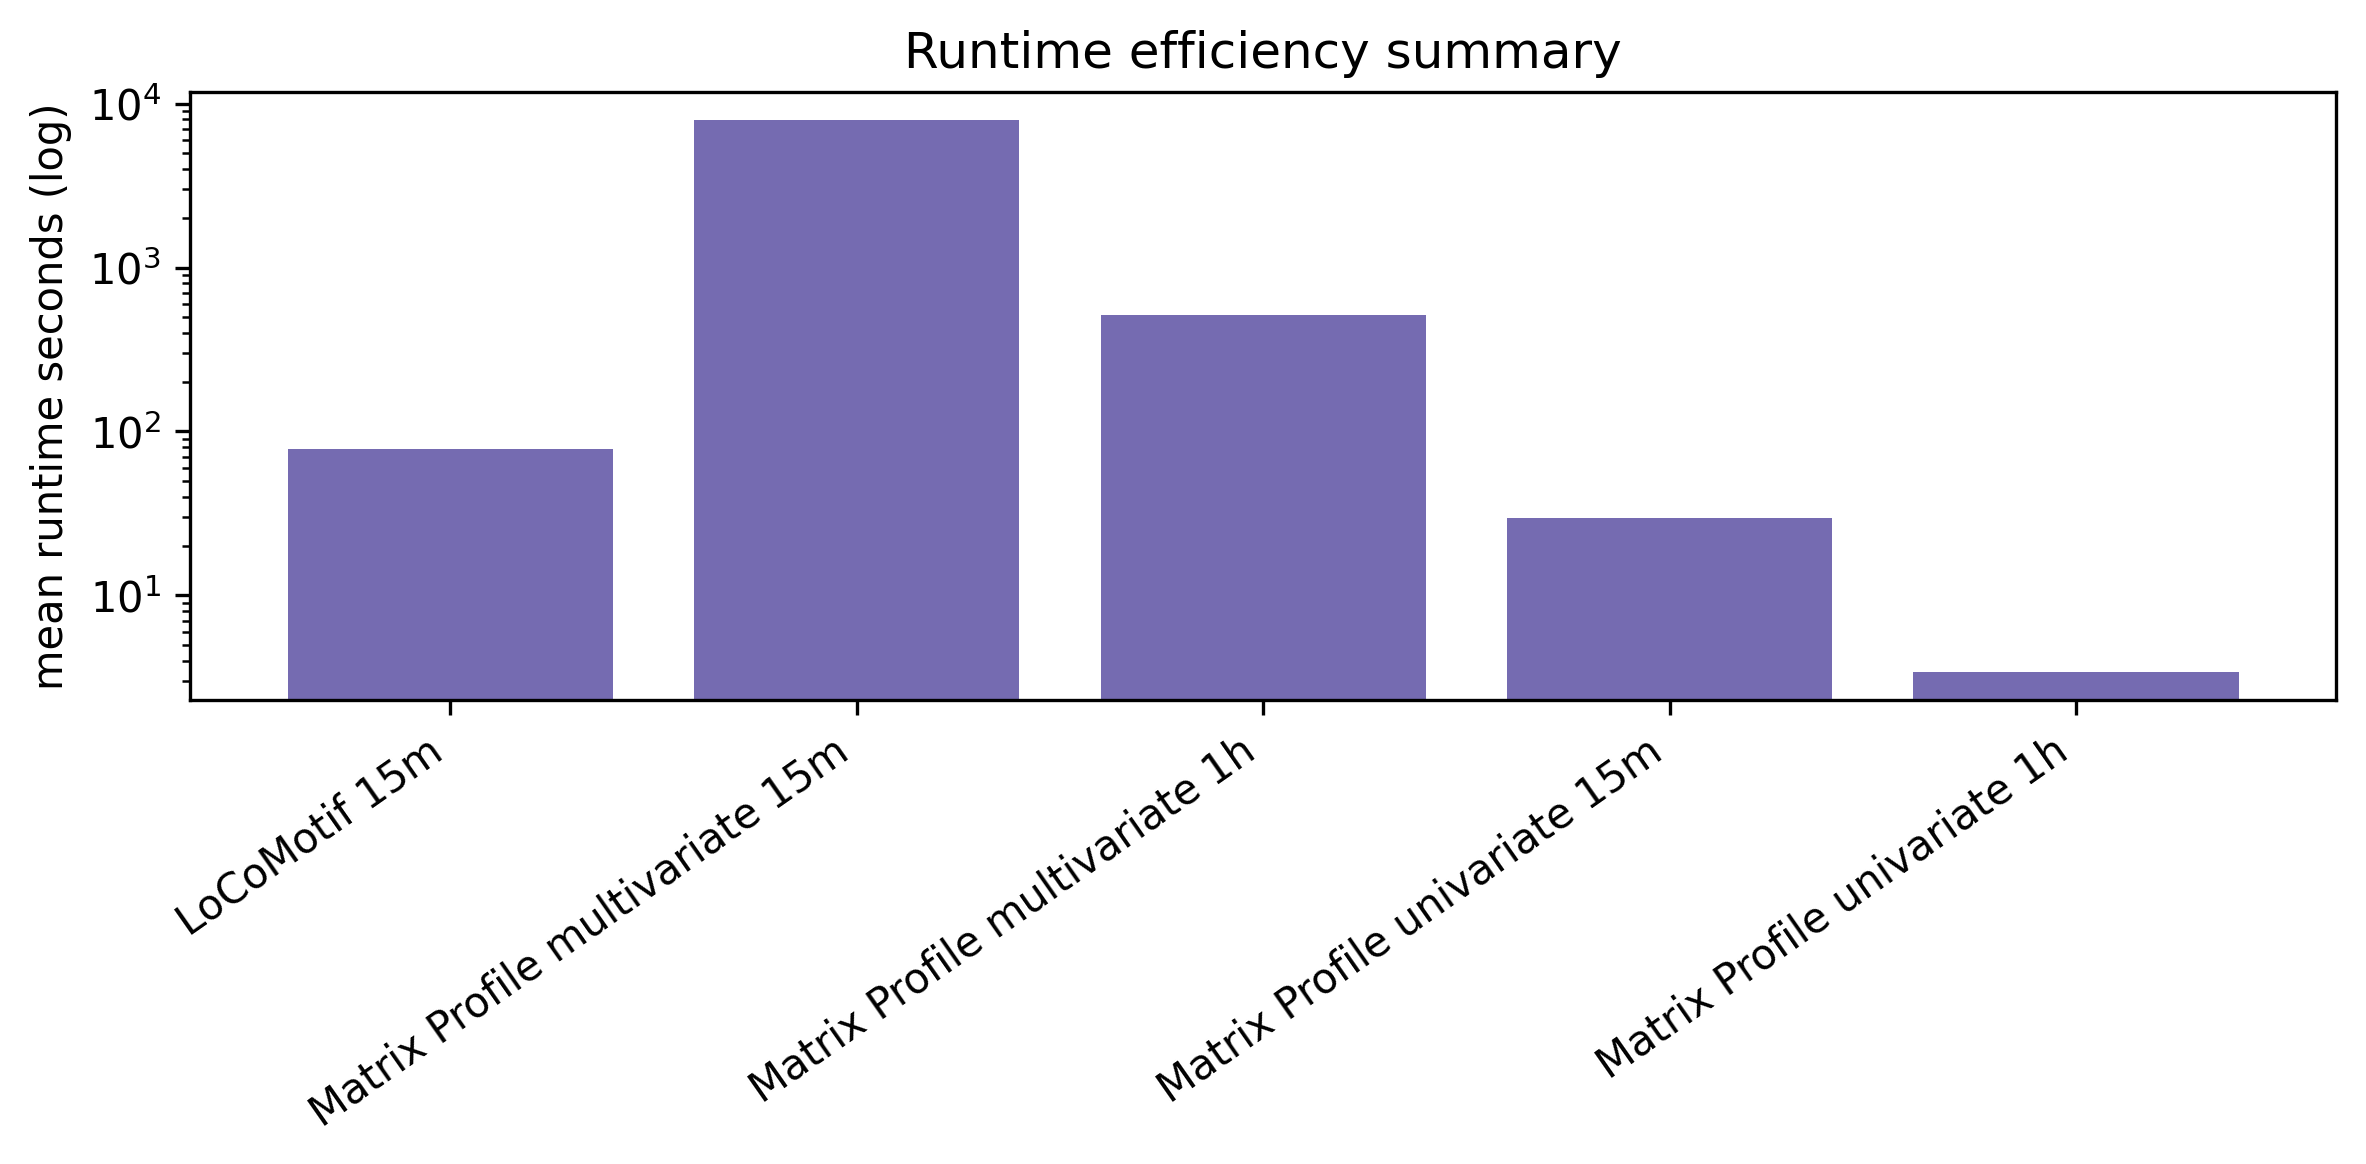
\includegraphics[width=0.9\linewidth]{reports/final_visual_evidence/figures/runtime_efficiency_summary_logscale.png}
\caption{runtime efficiency summary logscale.}
\end{figure}

\begin{figure}[ht]
\centering
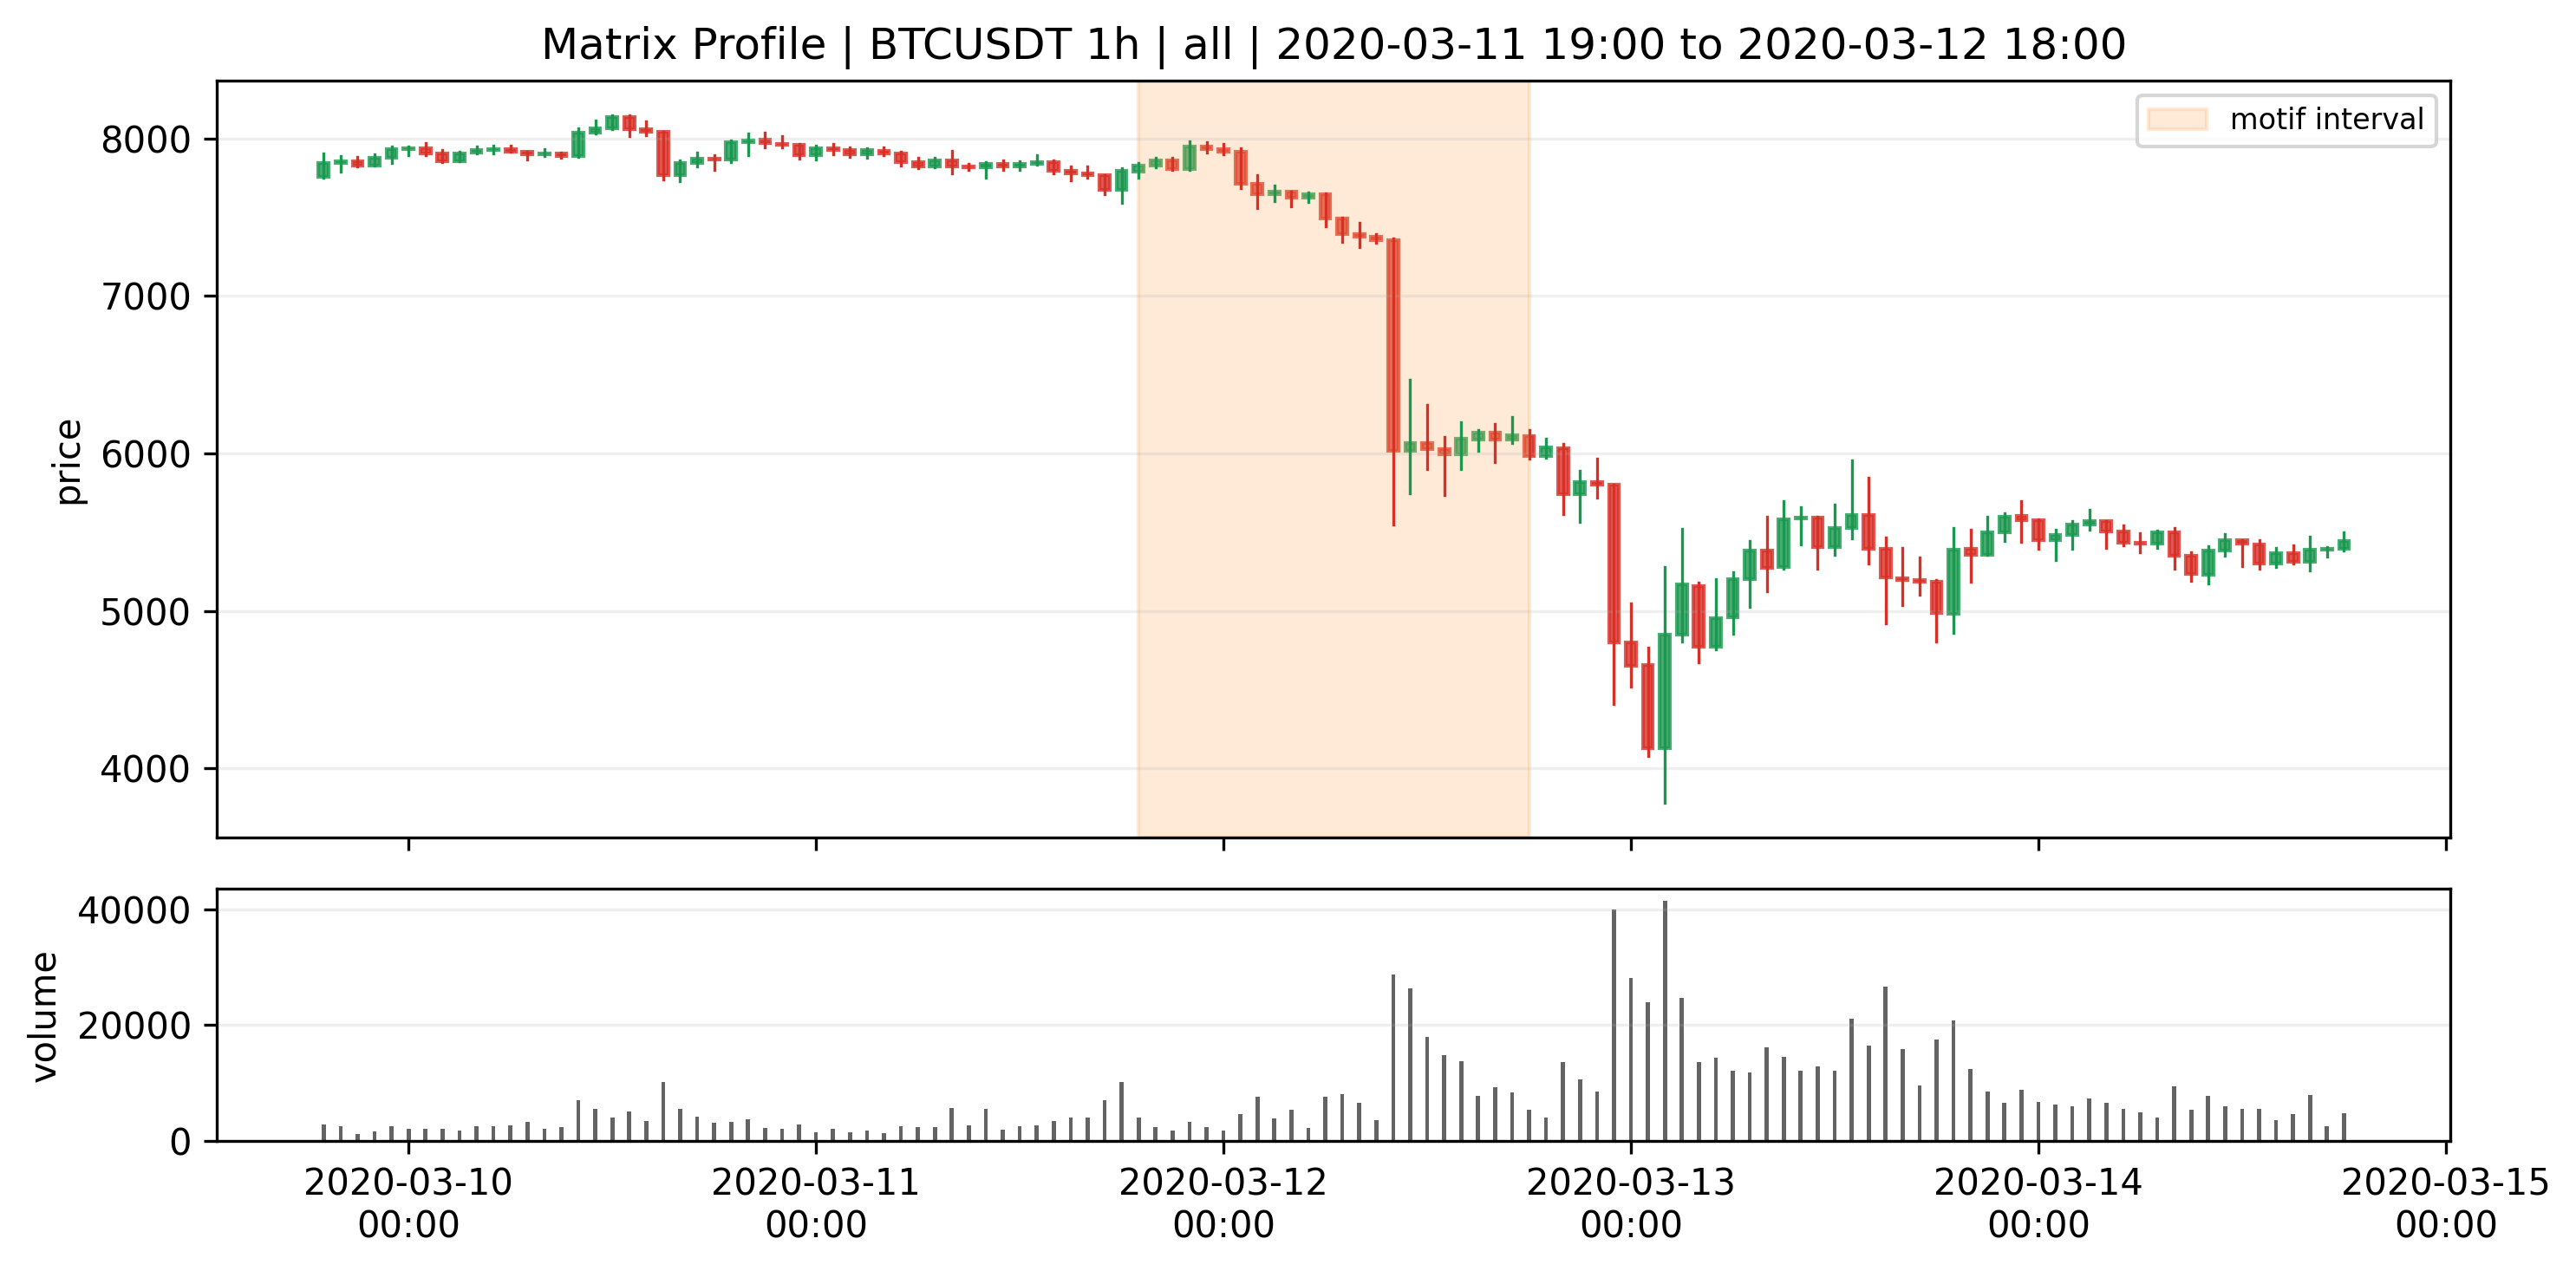
\includegraphics[width=0.9\linewidth]{reports/final_visual_evidence/figures/top_motif_01_matrix_profile_btcusdt_1h_all_context.png}
\caption{top motif 01 matrix profile btcusdt 1h all context. The shaded interval marks the discovered motif occurrence in original price context.}
\end{figure}

\begin{figure}[ht]
\centering
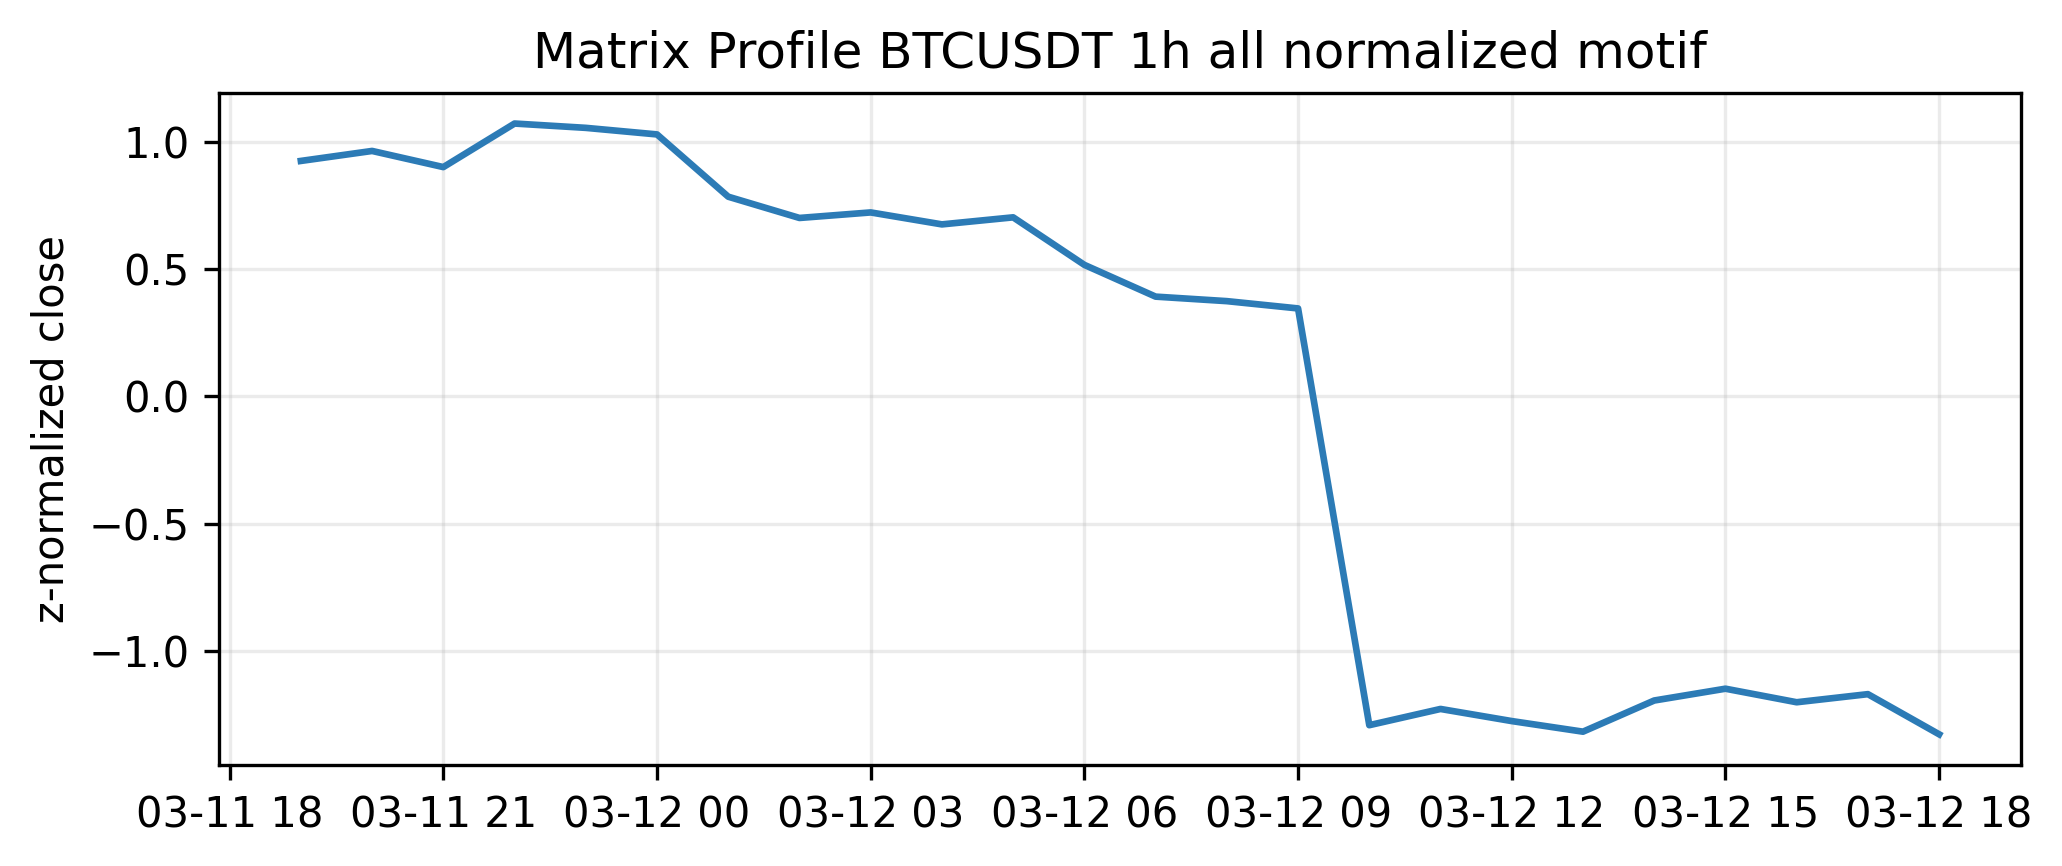
\includegraphics[width=0.9\linewidth]{reports/final_visual_evidence/figures/top_motif_01_matrix_profile_btcusdt_1h_all_normal_pattern.png}
\caption{top motif 01 matrix profile btcusdt 1h all normal pattern. The shaded interval marks the discovered motif occurrence in original price context.}
\end{figure}

\begin{figure}[ht]
\centering
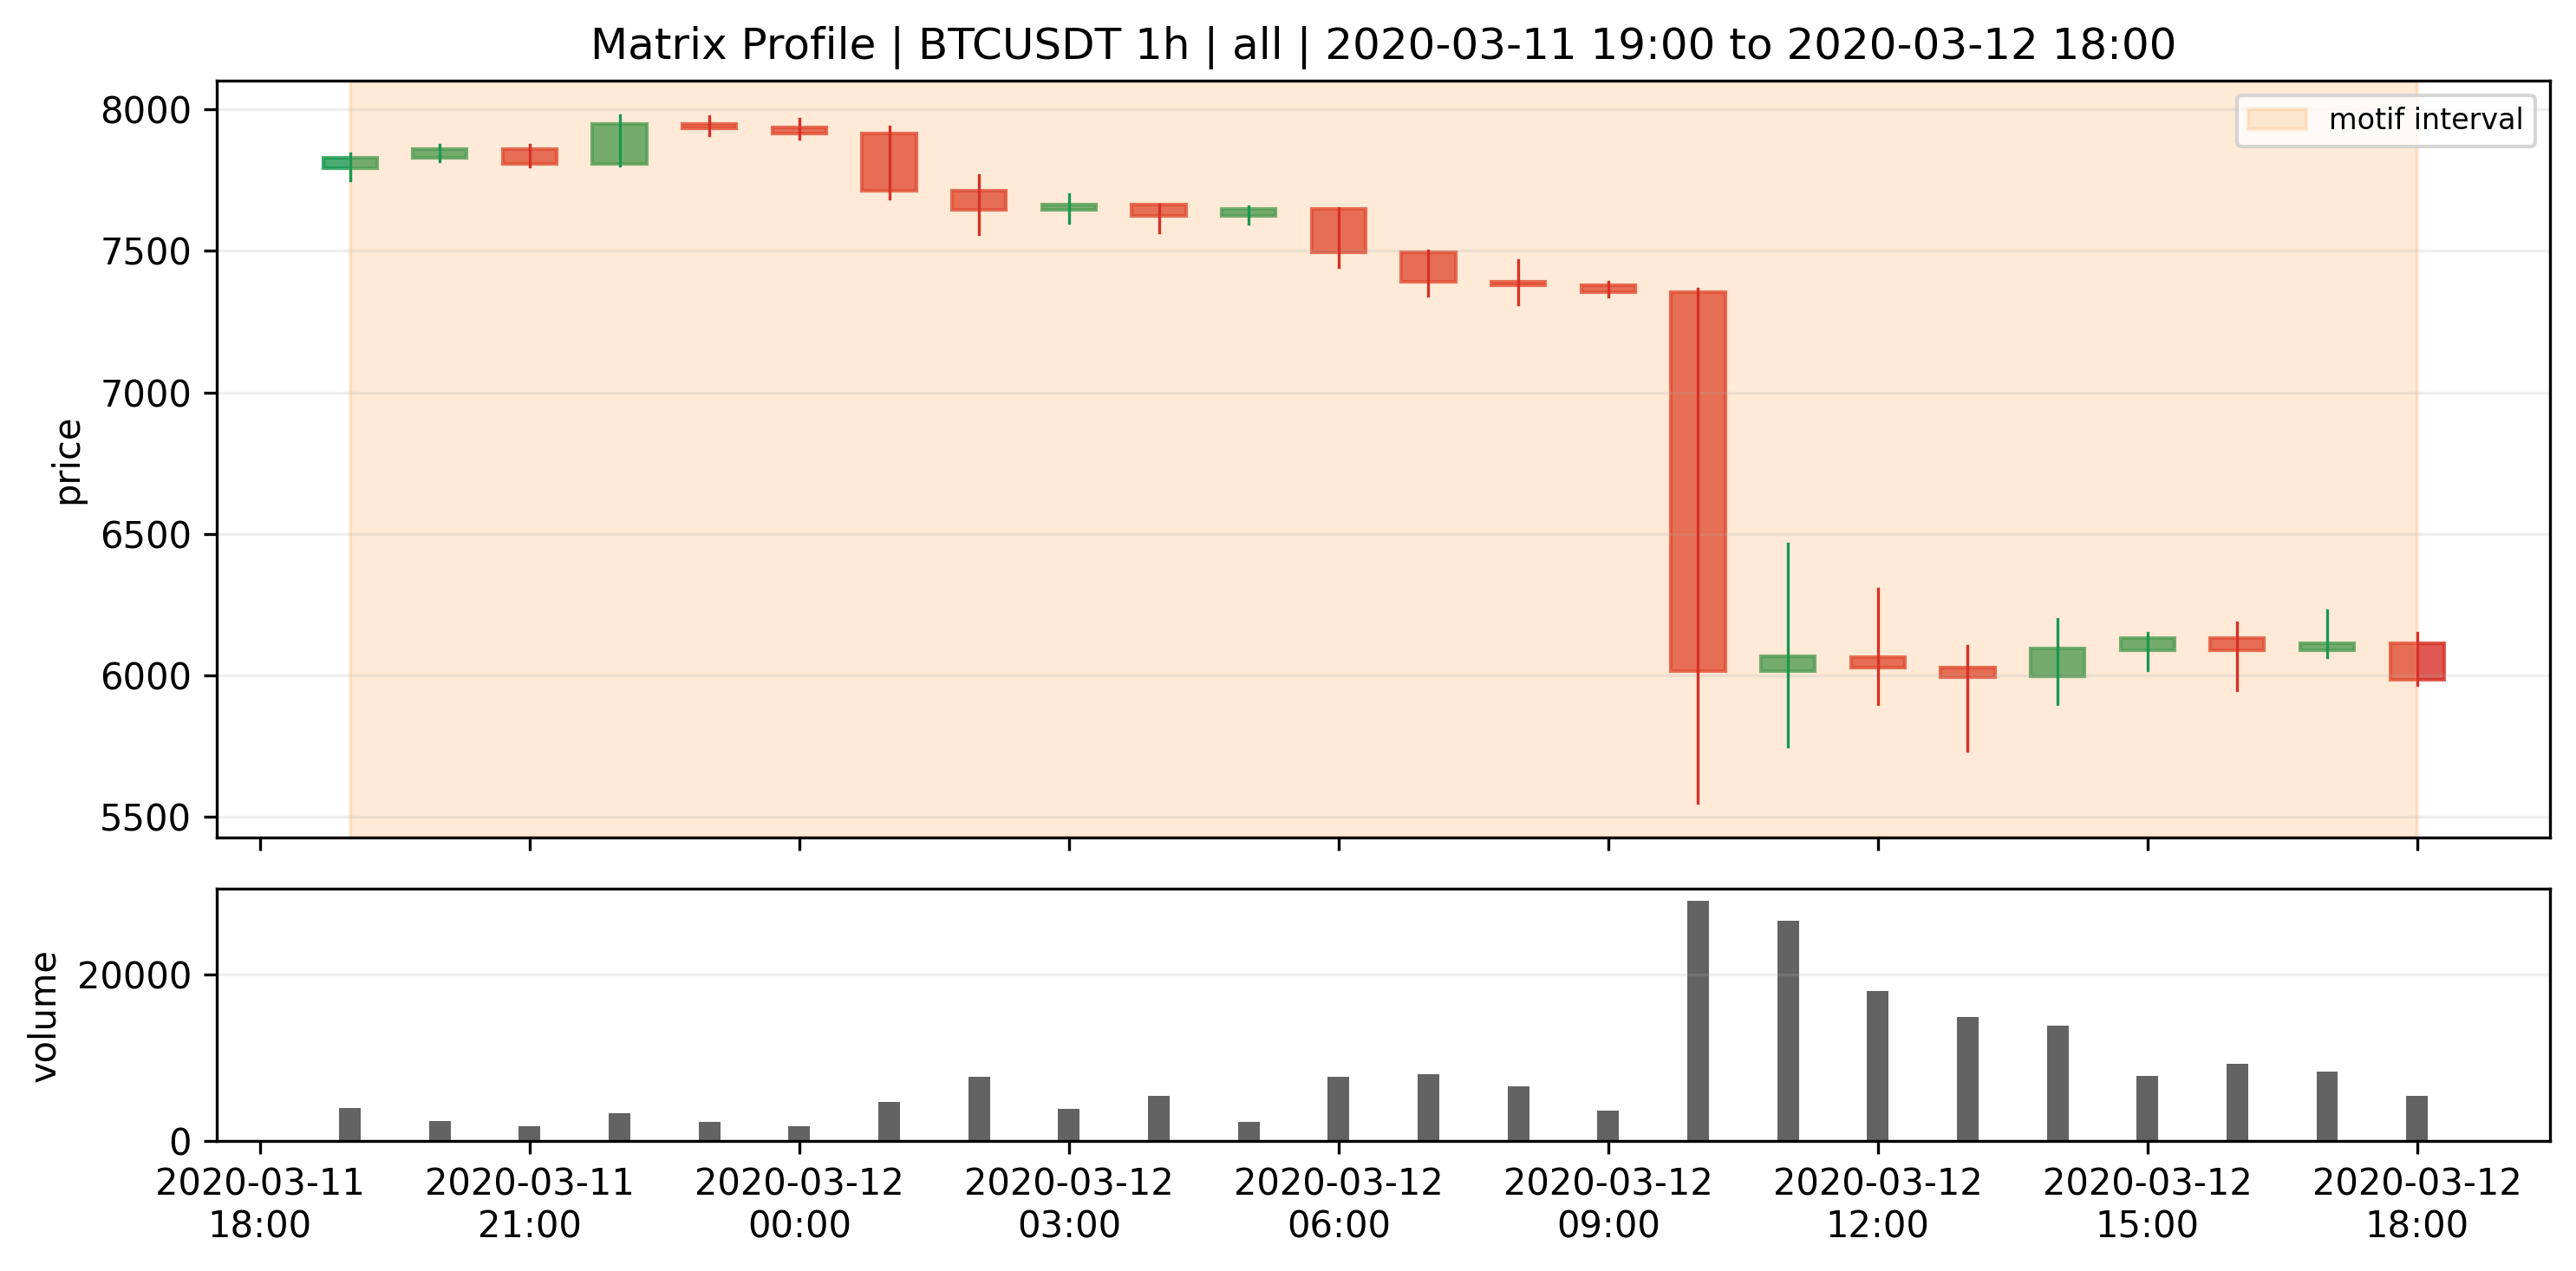
\includegraphics[width=0.9\linewidth]{reports/final_visual_evidence/figures/top_motif_01_matrix_profile_btcusdt_1h_all_zoom.png}
\caption{top motif 01 matrix profile btcusdt 1h all zoom. The shaded interval marks the discovered motif occurrence in original price context.}
\end{figure}

\begin{figure}[ht]
\centering
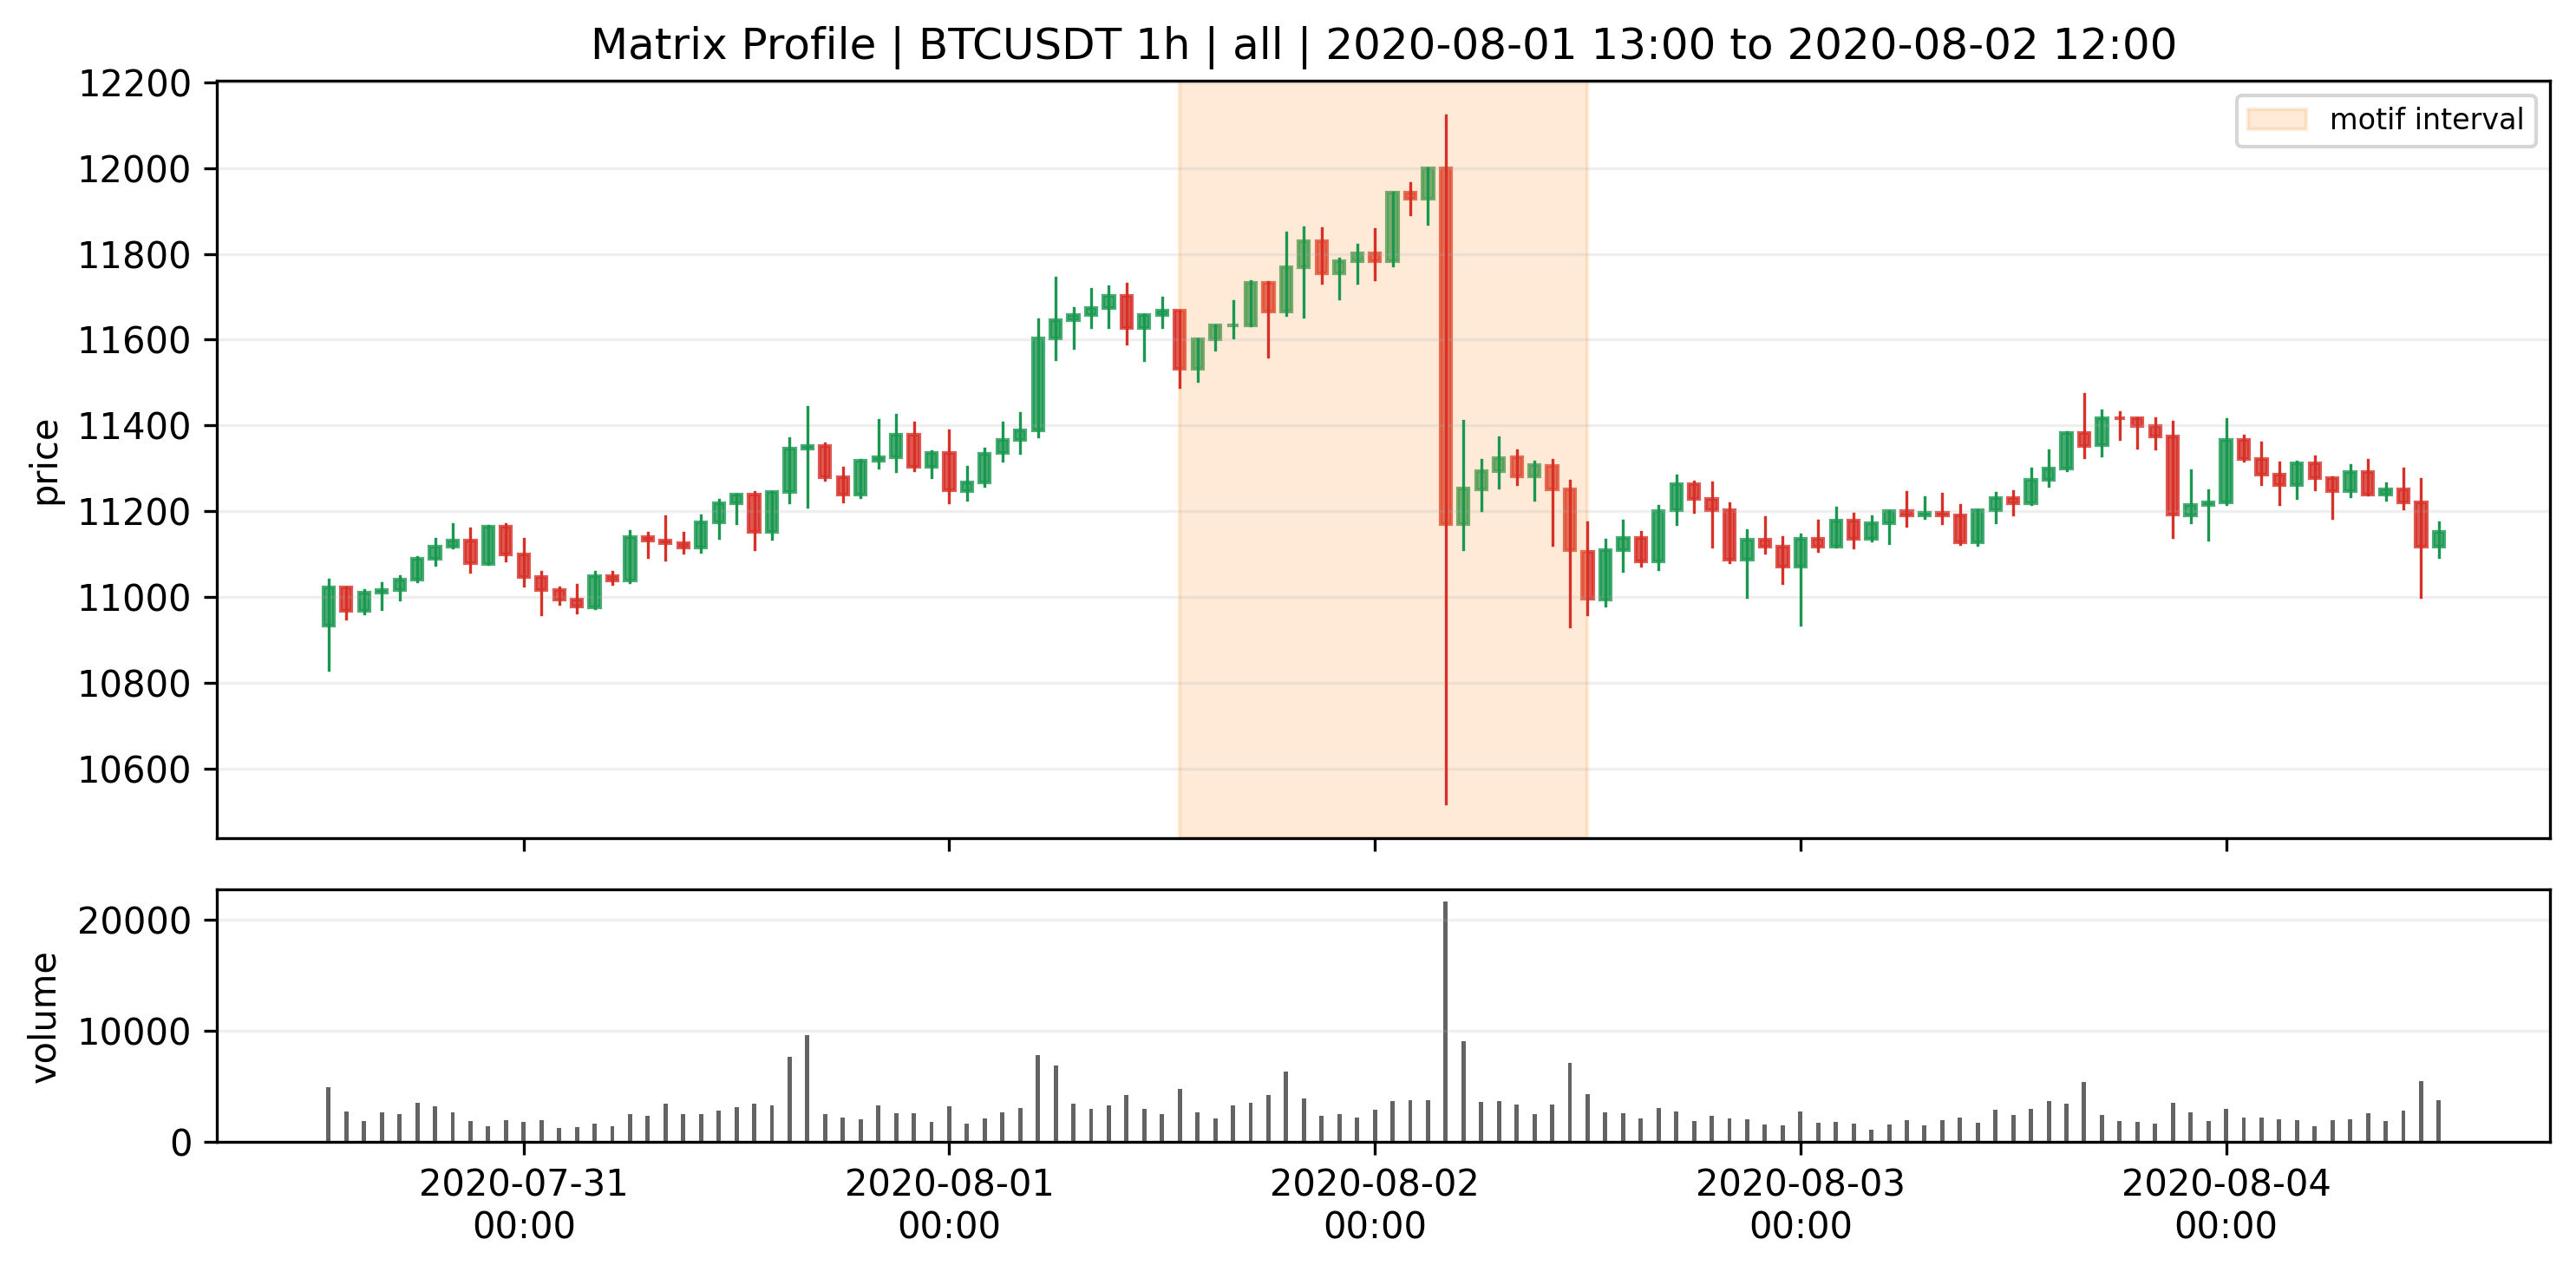
\includegraphics[width=0.9\linewidth]{reports/final_visual_evidence/figures/top_motif_02_matrix_profile_btcusdt_1h_all_context.png}
\caption{top motif 02 matrix profile btcusdt 1h all context. The shaded interval marks the discovered motif occurrence in original price context.}
\end{figure}

\begin{figure}[ht]
\centering
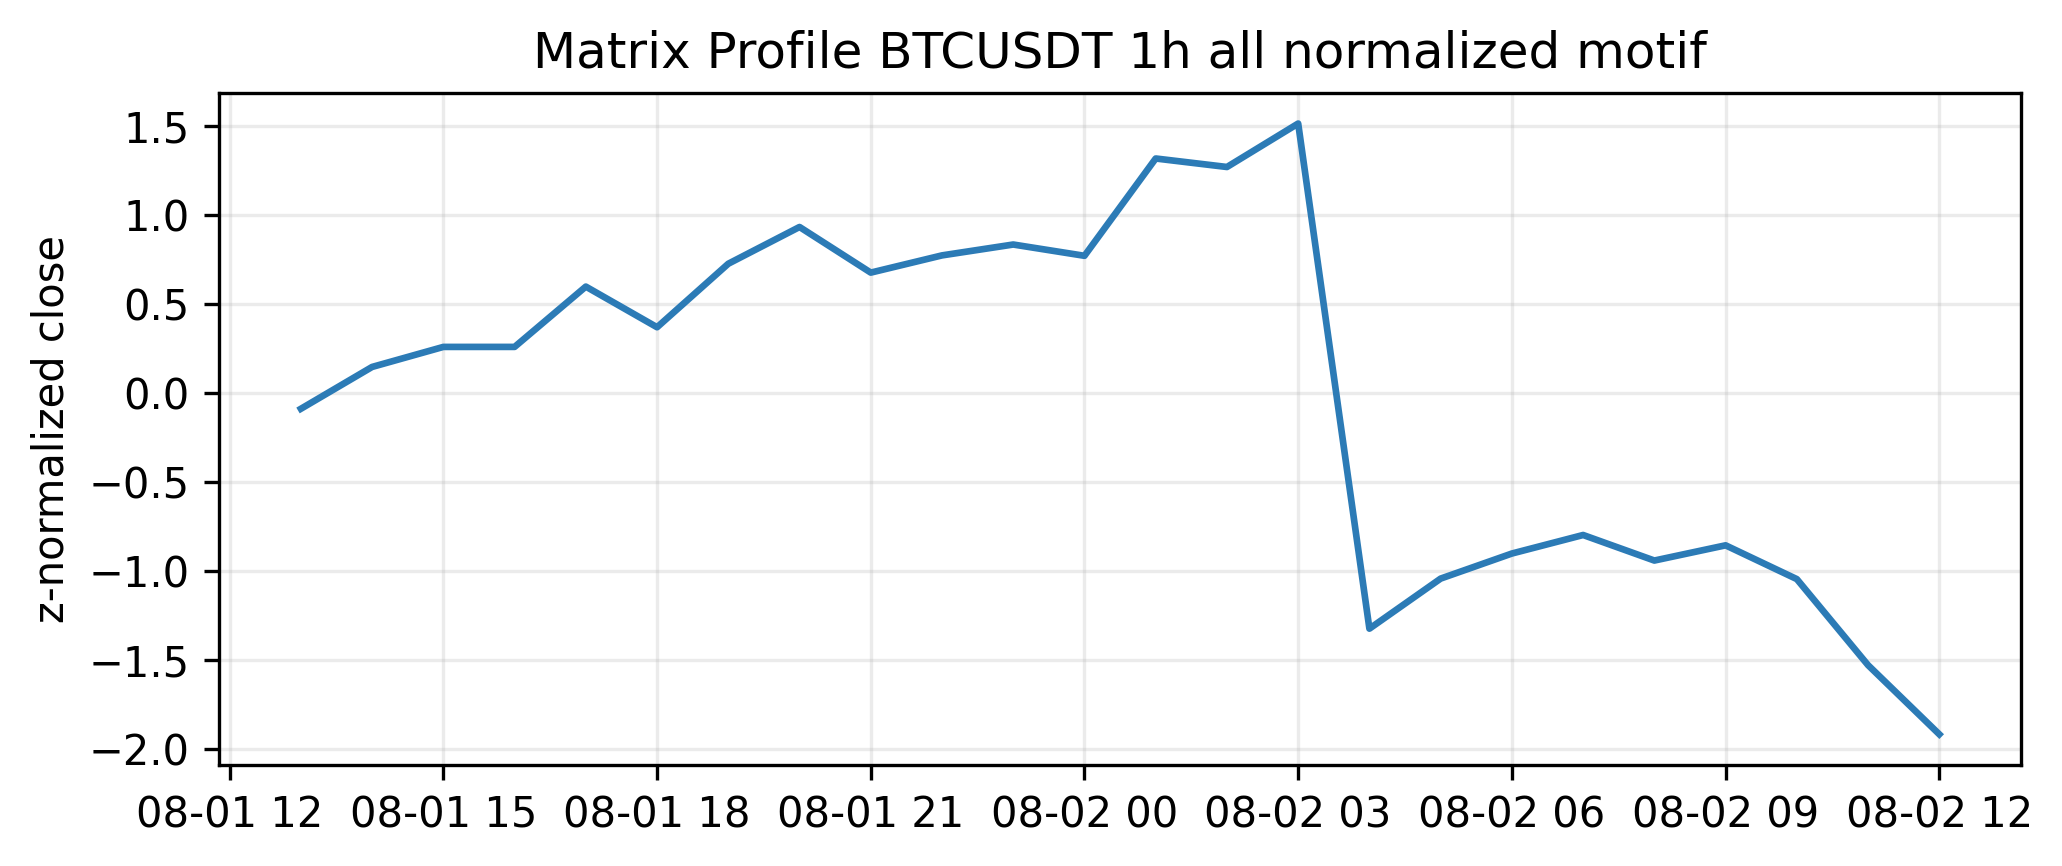
\includegraphics[width=0.9\linewidth]{reports/final_visual_evidence/figures/top_motif_02_matrix_profile_btcusdt_1h_all_normal_pattern.png}
\caption{top motif 02 matrix profile btcusdt 1h all normal pattern. The shaded interval marks the discovered motif occurrence in original price context.}
\end{figure}

\begin{figure}[ht]
\centering
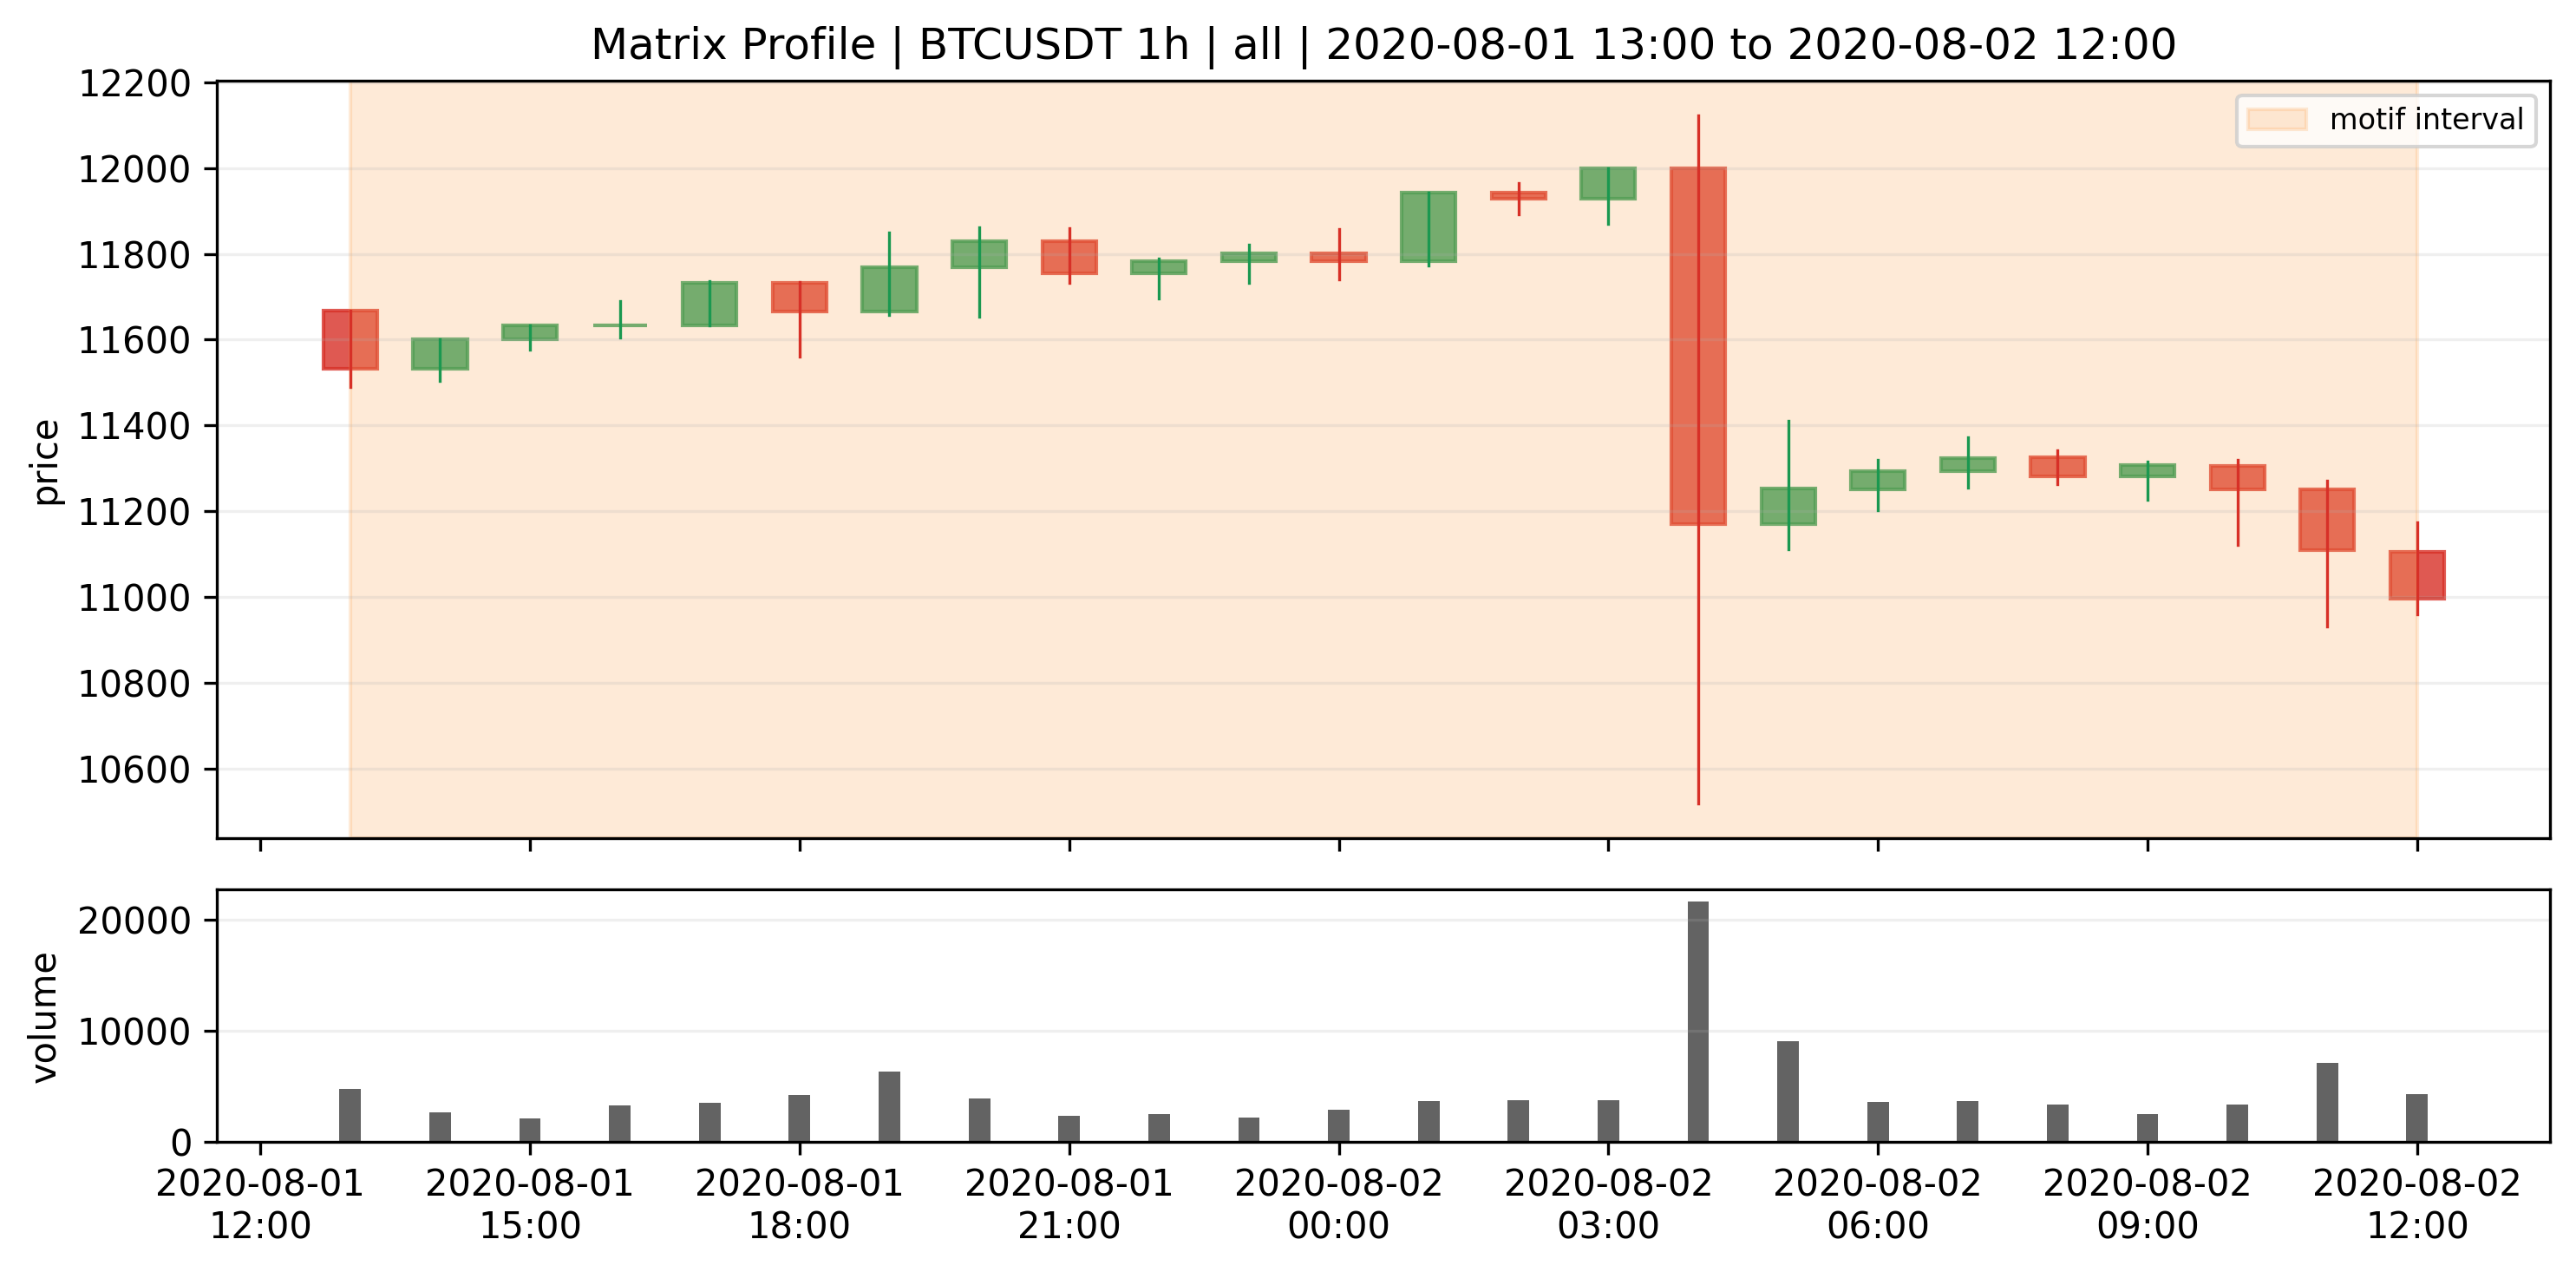
\includegraphics[width=0.9\linewidth]{reports/final_visual_evidence/figures/top_motif_02_matrix_profile_btcusdt_1h_all_zoom.png}
\caption{top motif 02 matrix profile btcusdt 1h all zoom. The shaded interval marks the discovered motif occurrence in original price context.}
\end{figure}

\begin{figure}[ht]
\centering
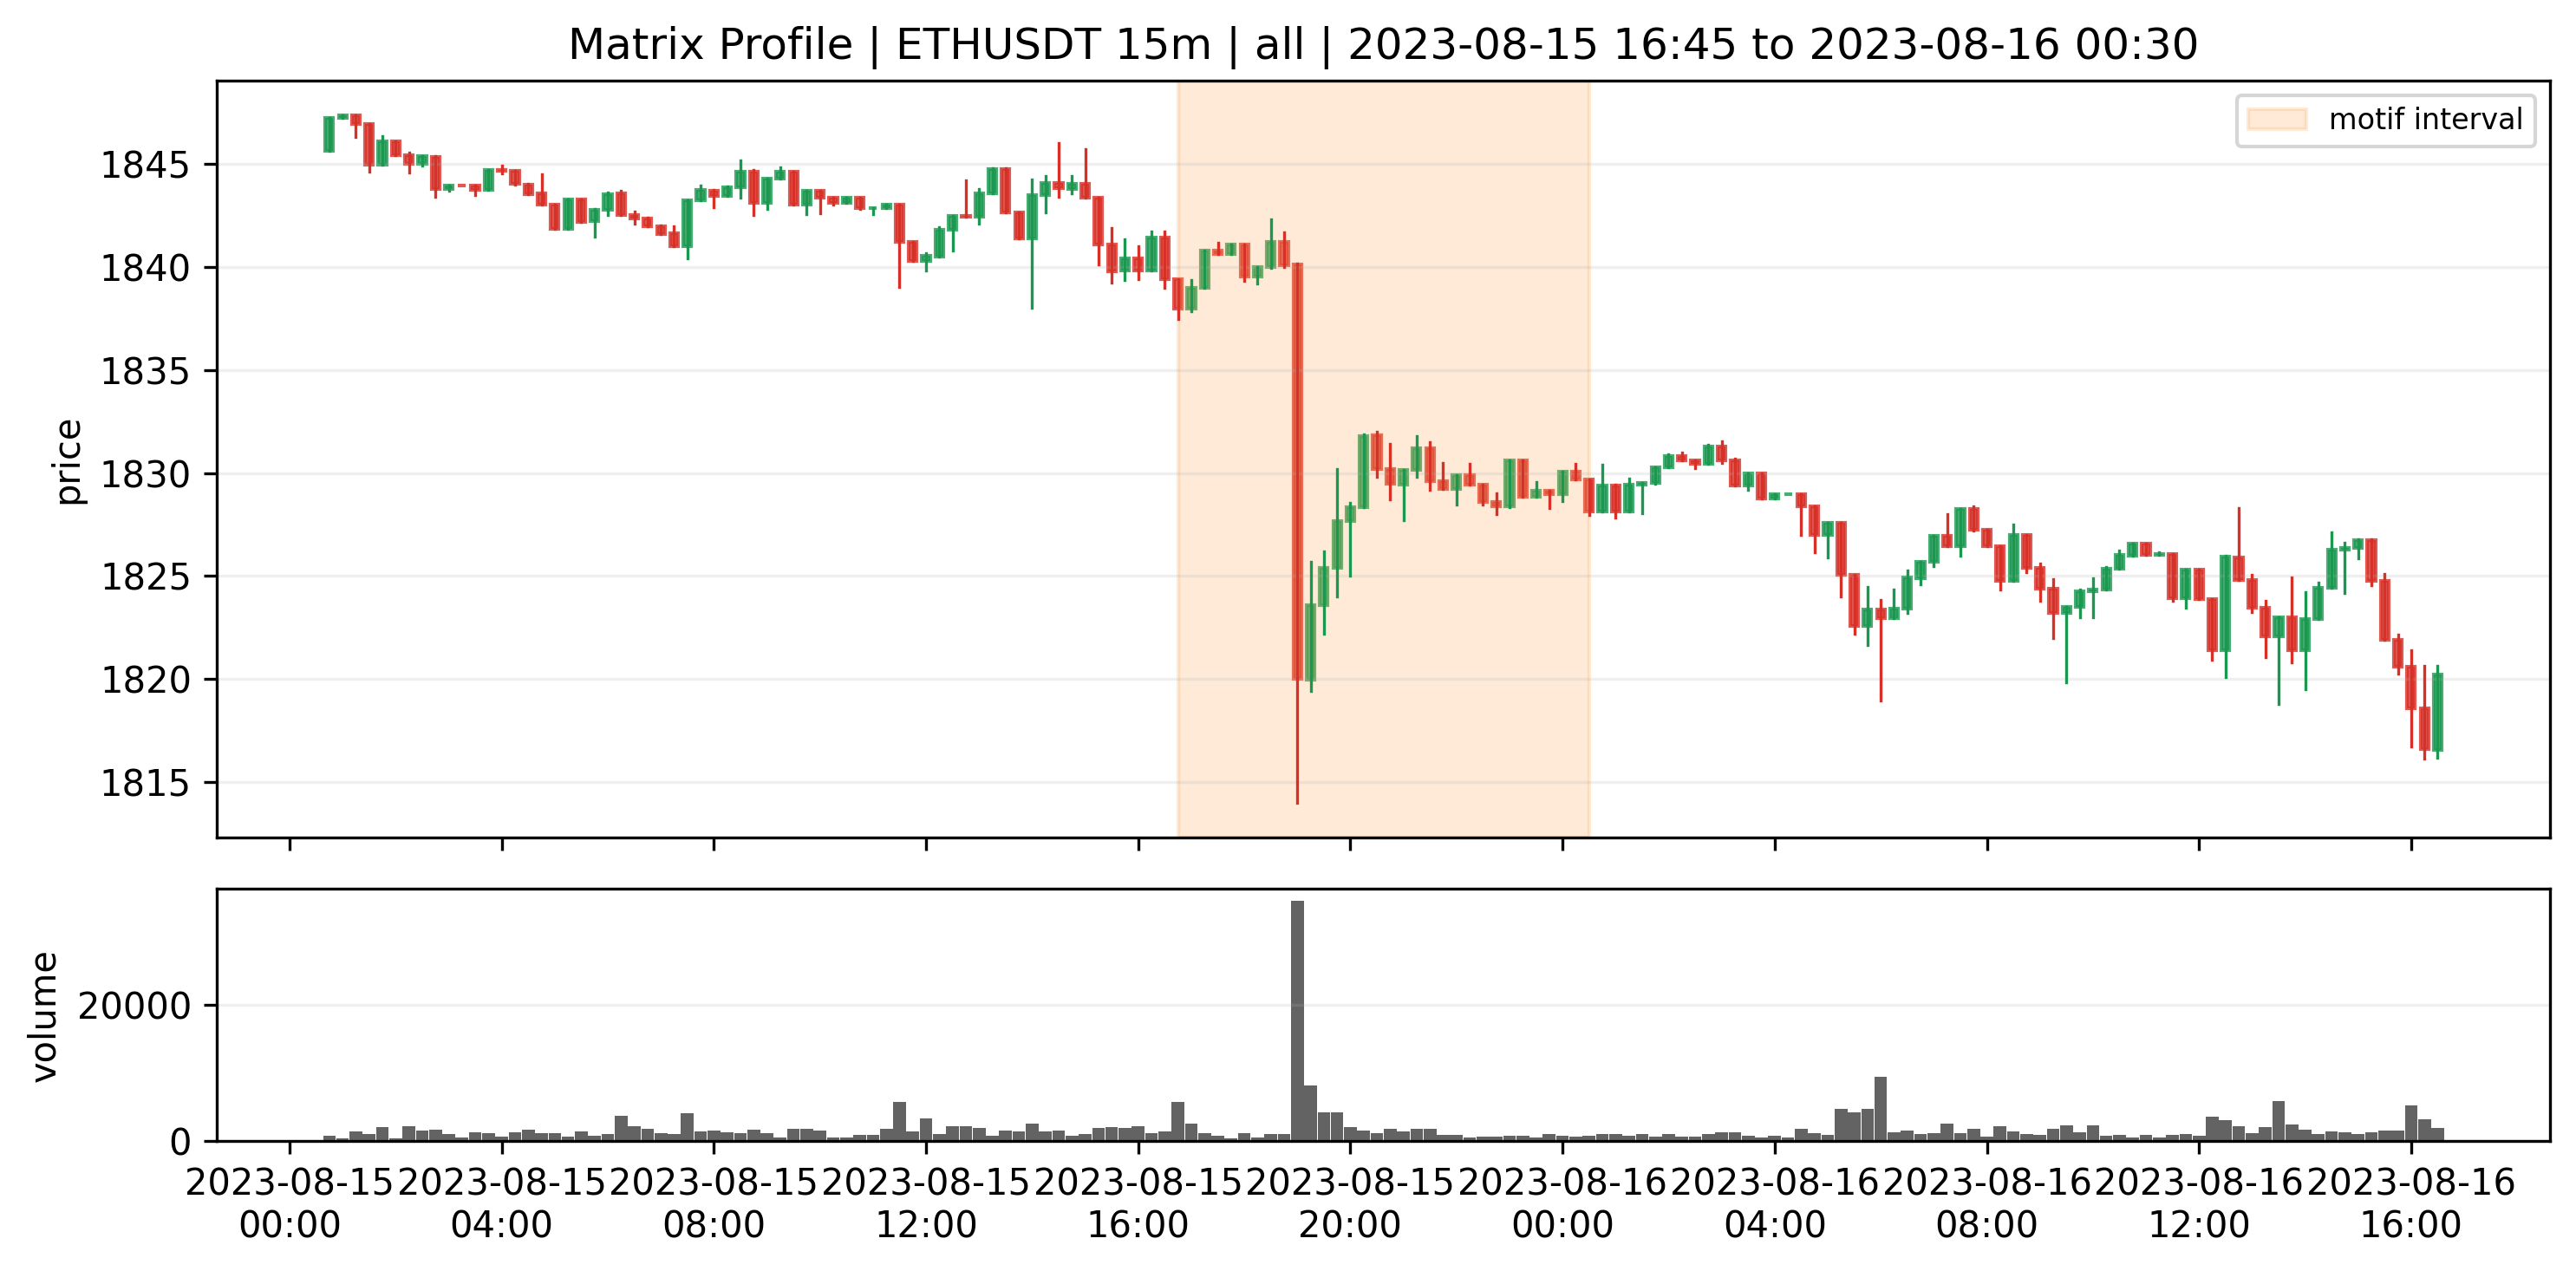
\includegraphics[width=0.9\linewidth]{reports/final_visual_evidence/figures/top_motif_03_matrix_profile_ethusdt_15m_all_context.png}
\caption{top motif 03 matrix profile ethusdt 15m all context. The shaded interval marks the discovered motif occurrence in original price context.}
\end{figure}

\begin{figure}[ht]
\centering
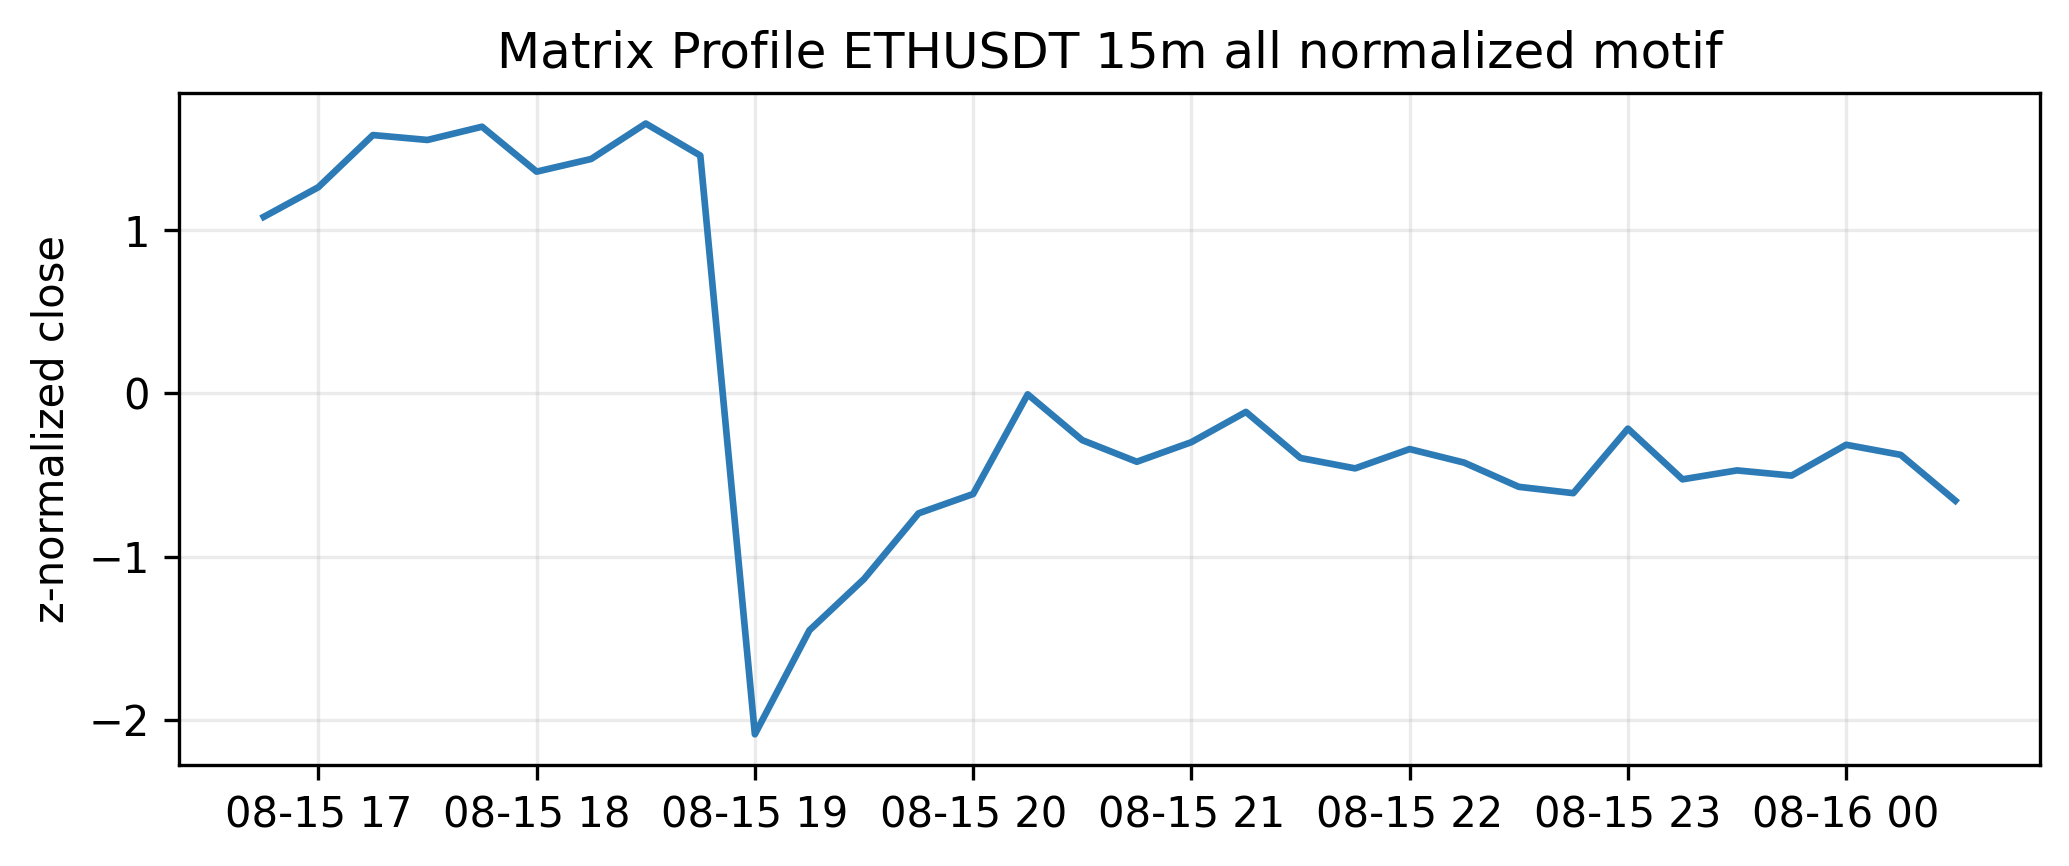
\includegraphics[width=0.9\linewidth]{reports/final_visual_evidence/figures/top_motif_03_matrix_profile_ethusdt_15m_all_normal_pattern.png}
\caption{top motif 03 matrix profile ethusdt 15m all normal pattern. The shaded interval marks the discovered motif occurrence in original price context.}
\end{figure}

\begin{figure}[ht]
\centering
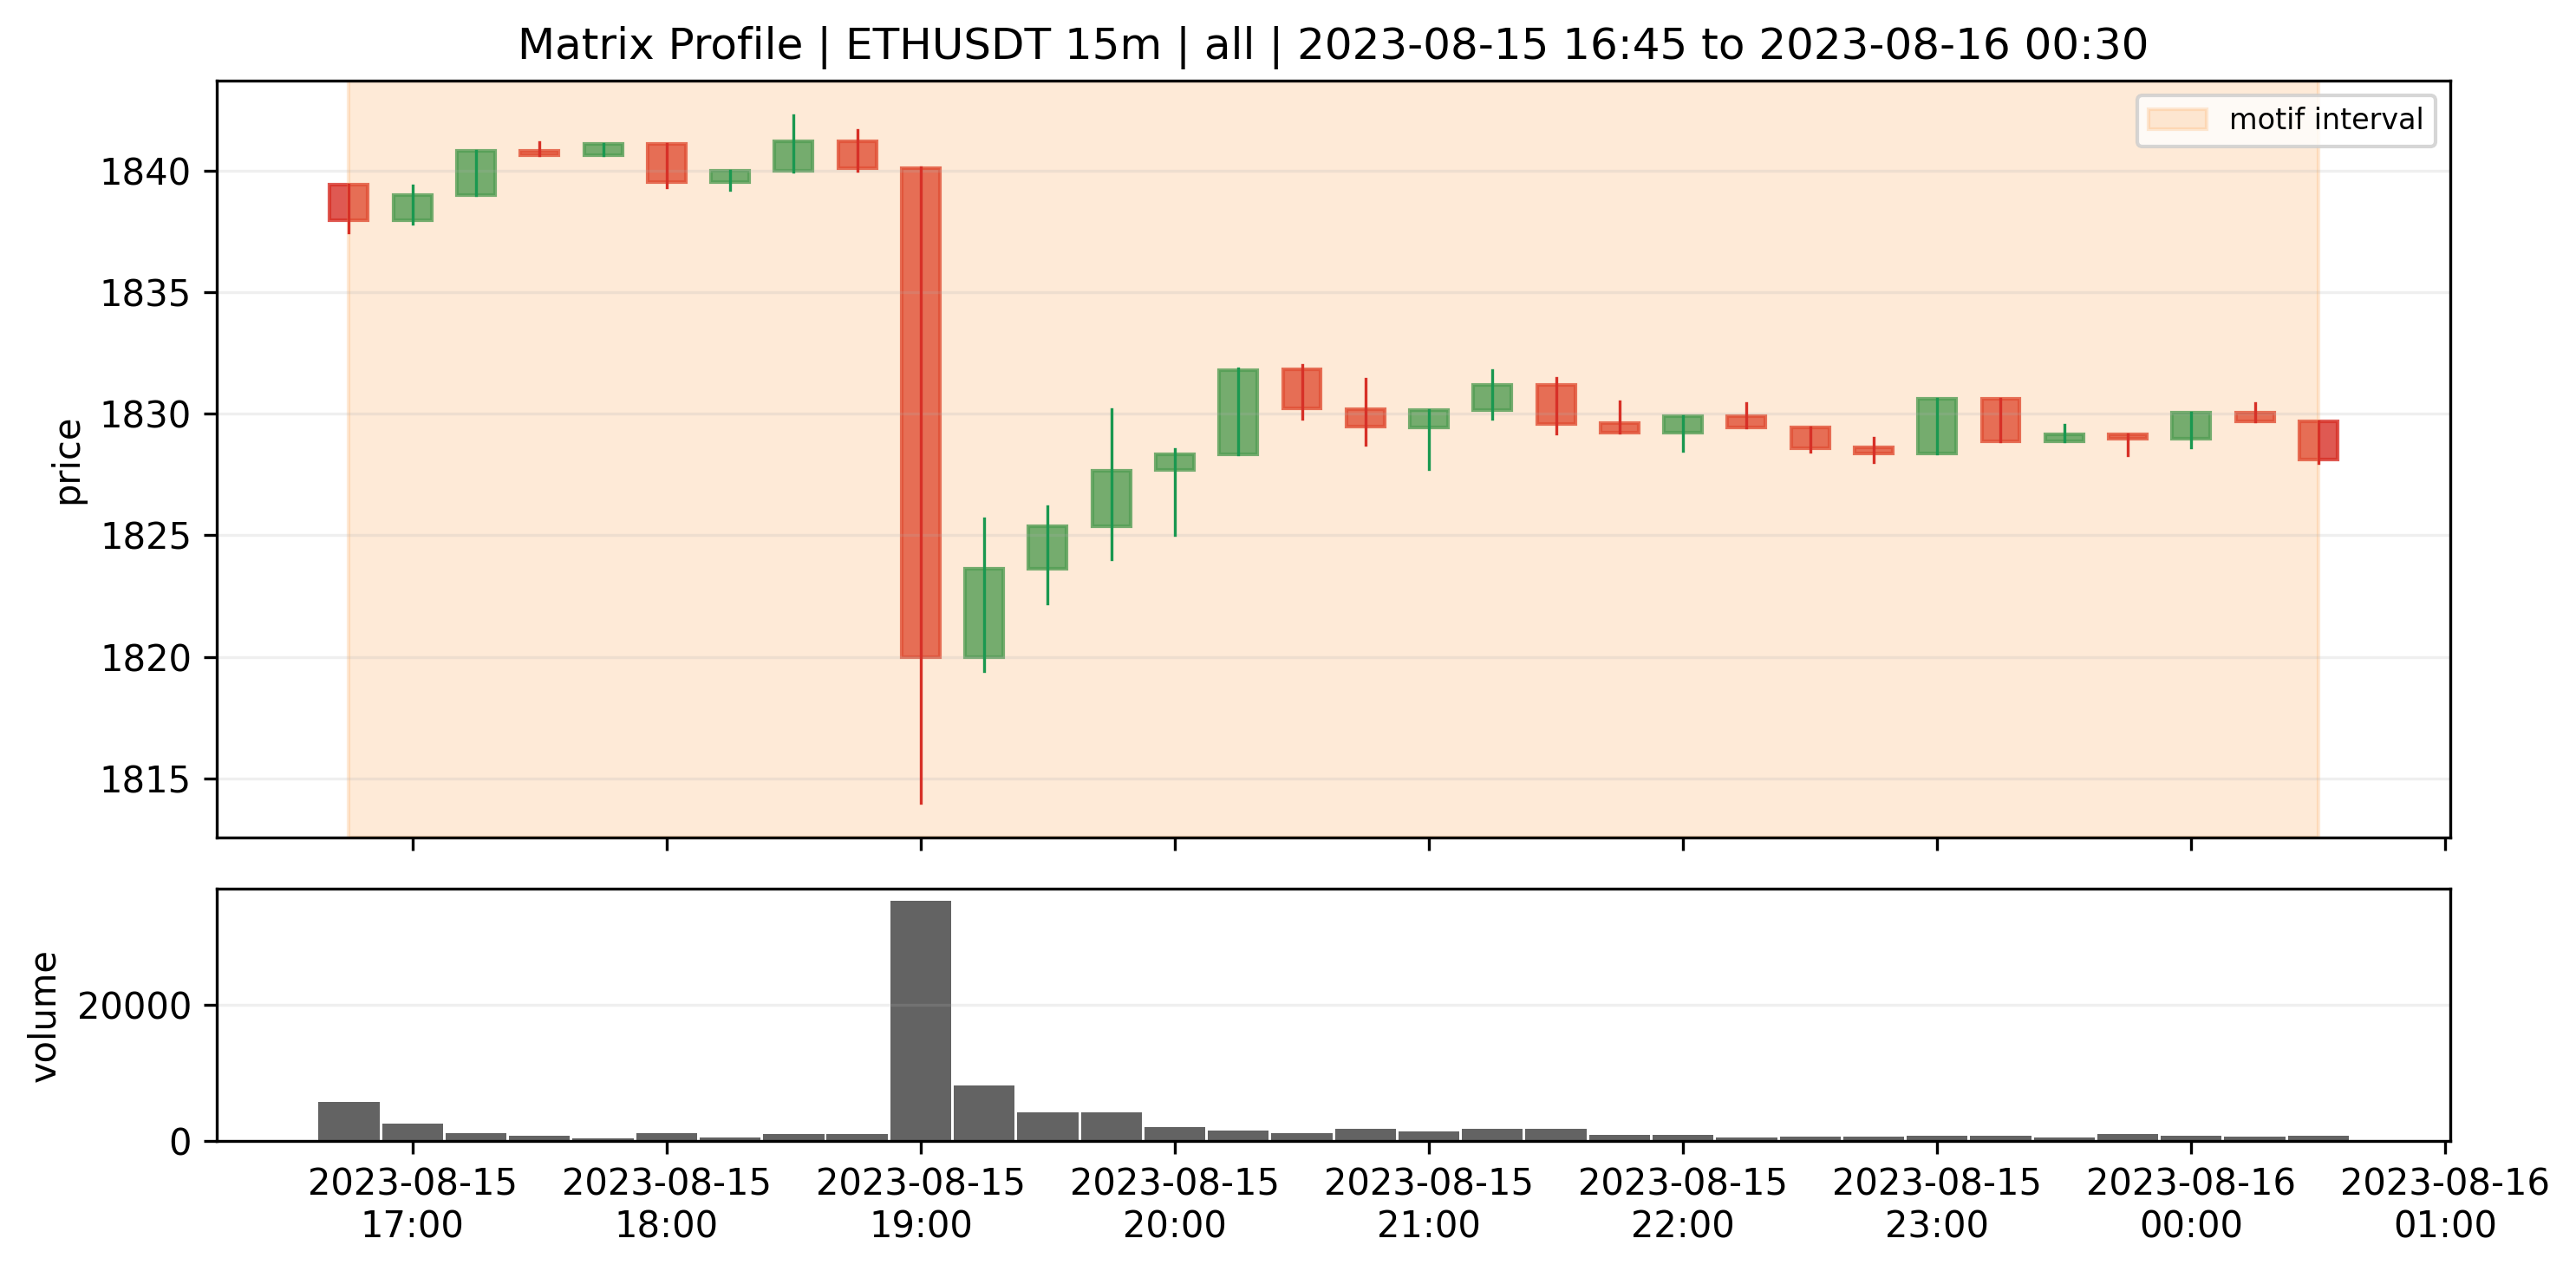
\includegraphics[width=0.9\linewidth]{reports/final_visual_evidence/figures/top_motif_03_matrix_profile_ethusdt_15m_all_zoom.png}
\caption{top motif 03 matrix profile ethusdt 15m all zoom. The shaded interval marks the discovered motif occurrence in original price context.}
\end{figure}

\begin{figure}[ht]
\centering
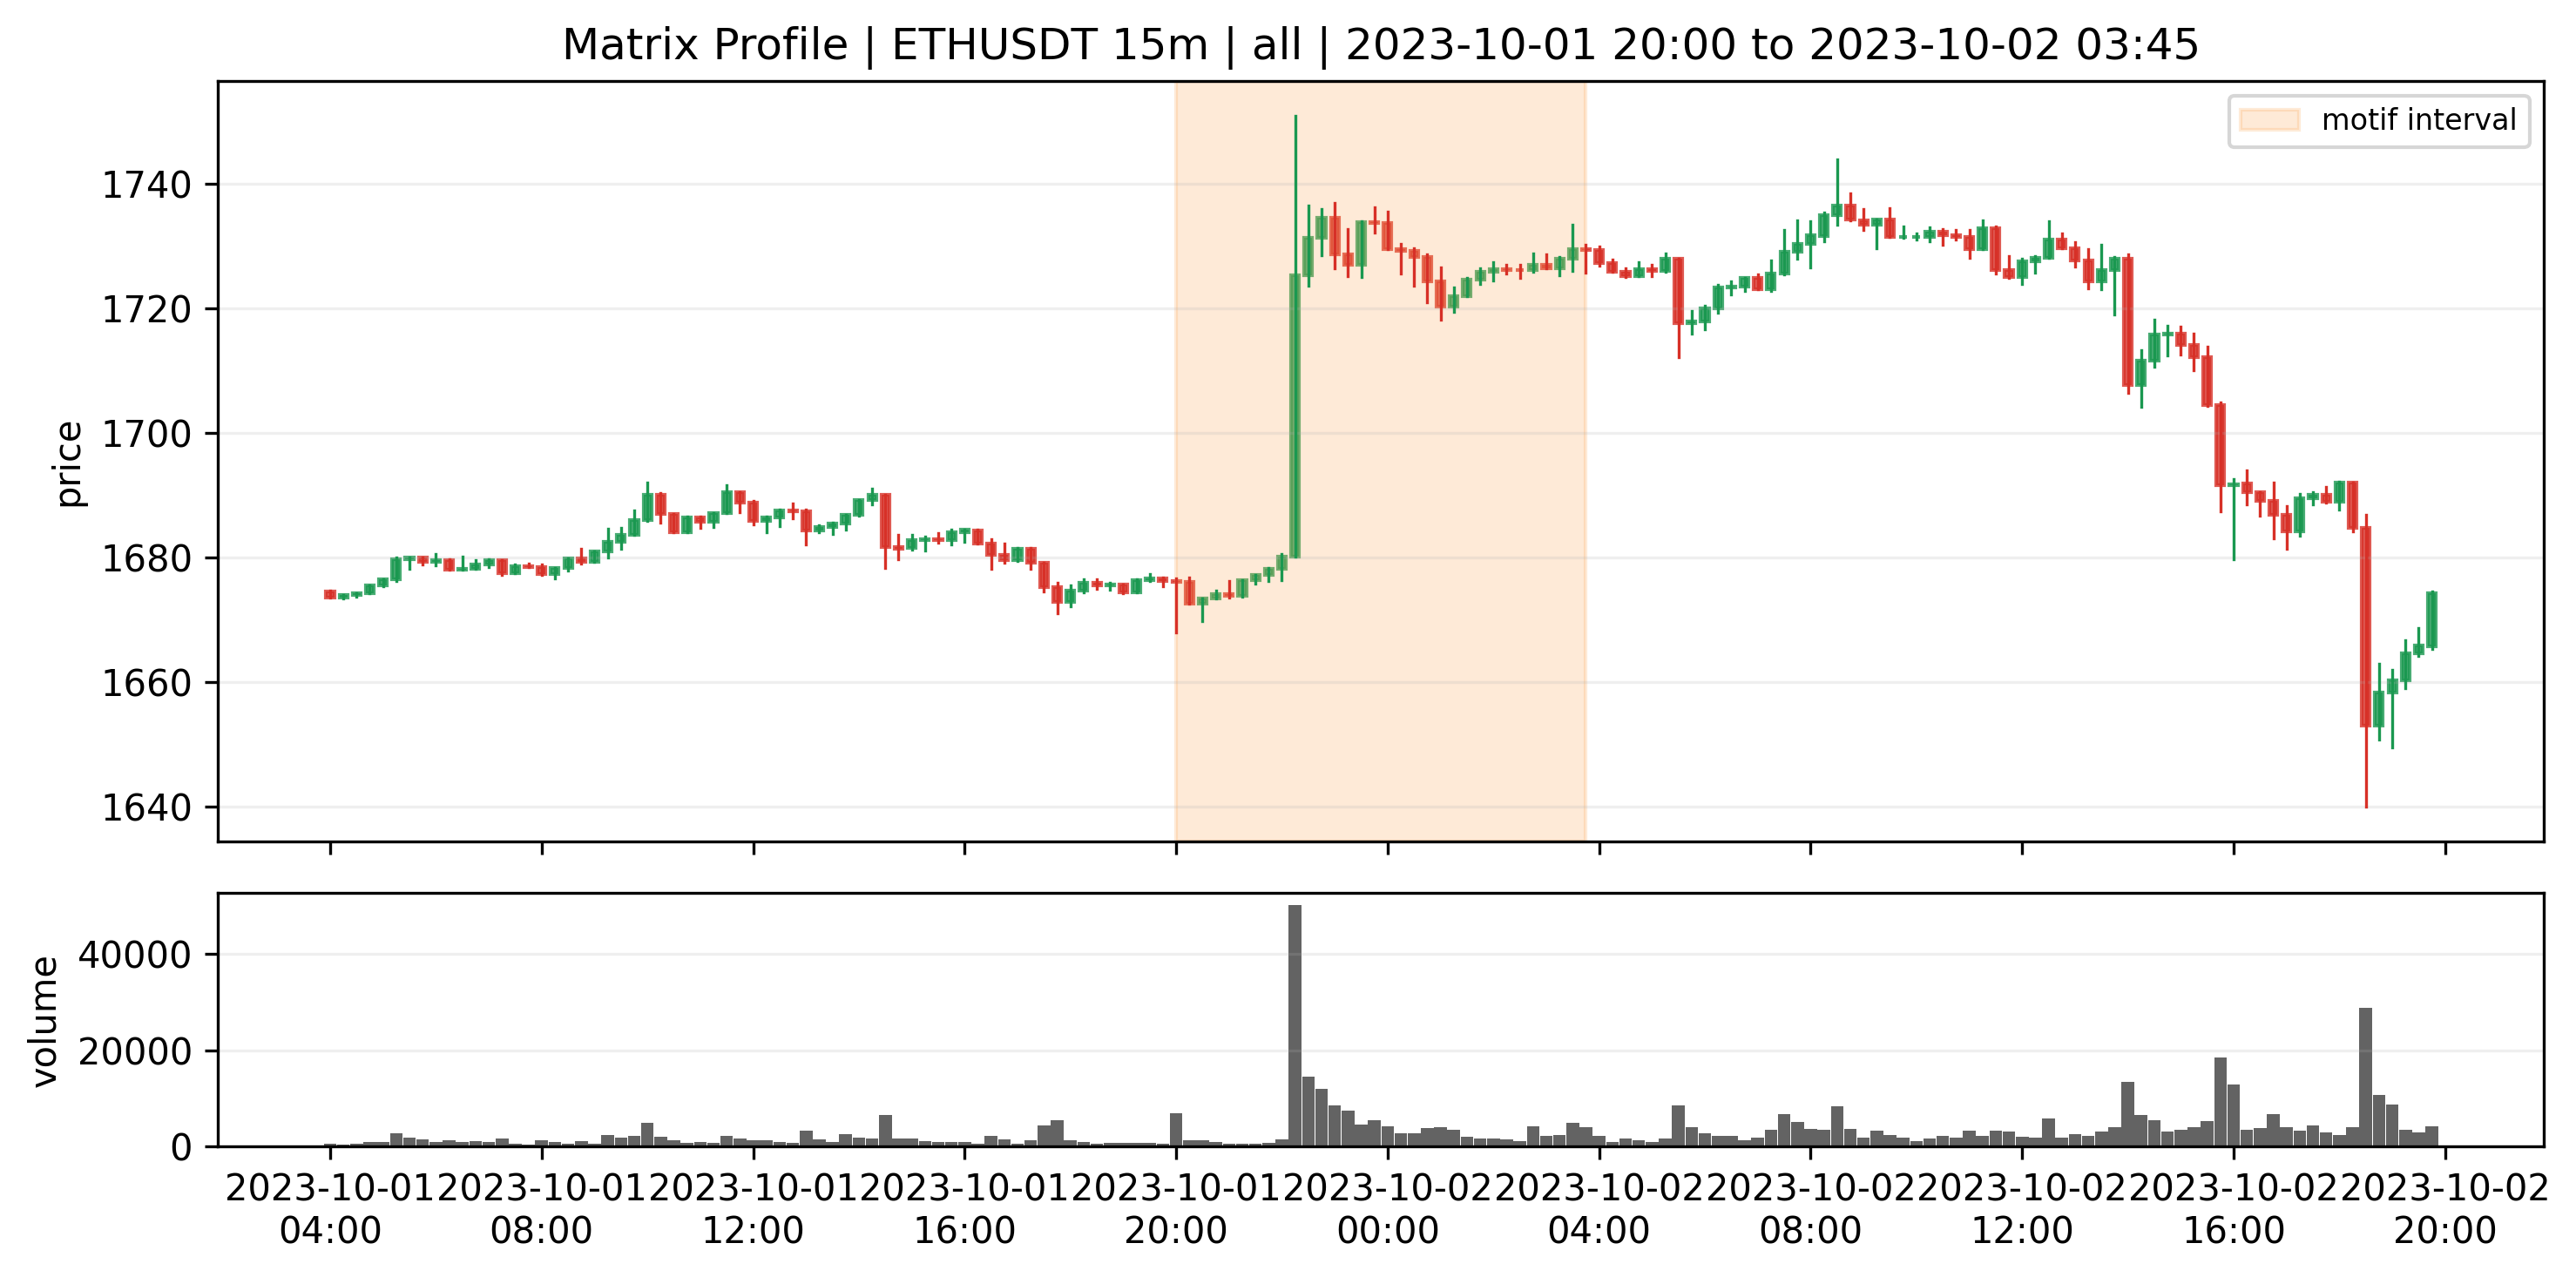
\includegraphics[width=0.9\linewidth]{reports/final_visual_evidence/figures/top_motif_04_matrix_profile_ethusdt_15m_all_context.png}
\caption{top motif 04 matrix profile ethusdt 15m all context. The shaded interval marks the discovered motif occurrence in original price context.}
\end{figure}

\begin{figure}[ht]
\centering
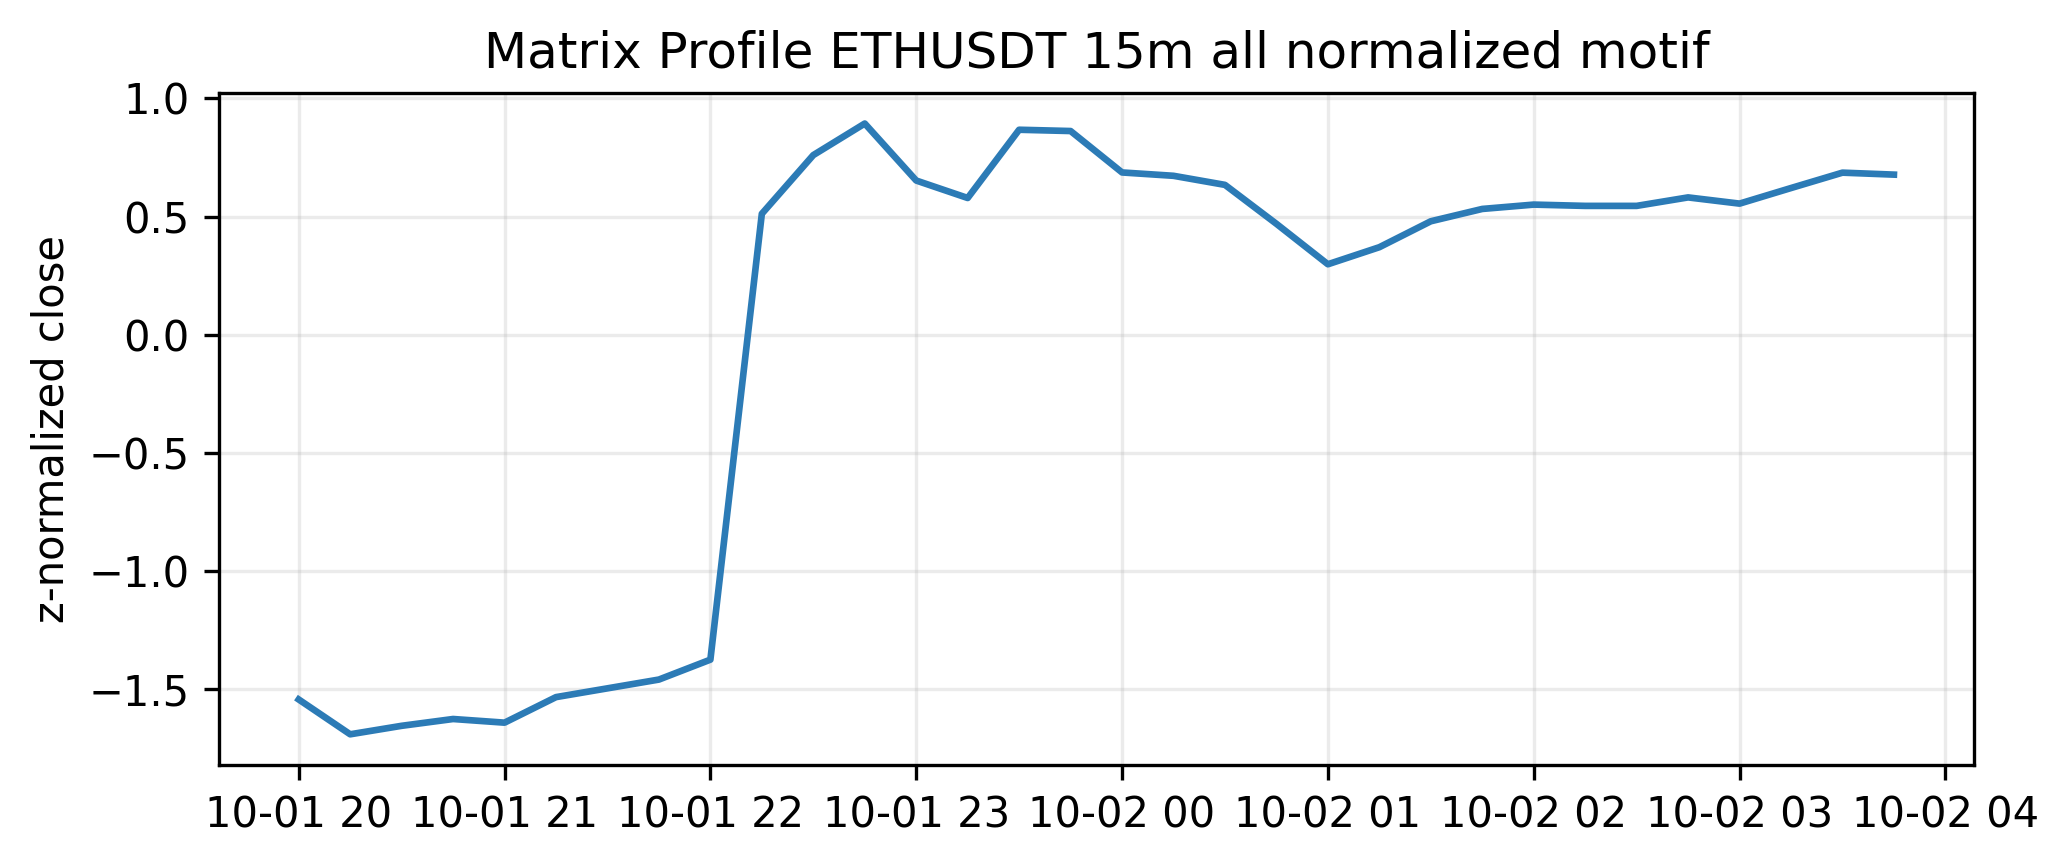
\includegraphics[width=0.9\linewidth]{reports/final_visual_evidence/figures/top_motif_04_matrix_profile_ethusdt_15m_all_normal_pattern.png}
\caption{top motif 04 matrix profile ethusdt 15m all normal pattern. The shaded interval marks the discovered motif occurrence in original price context.}
\end{figure}

\begin{figure}[ht]
\centering
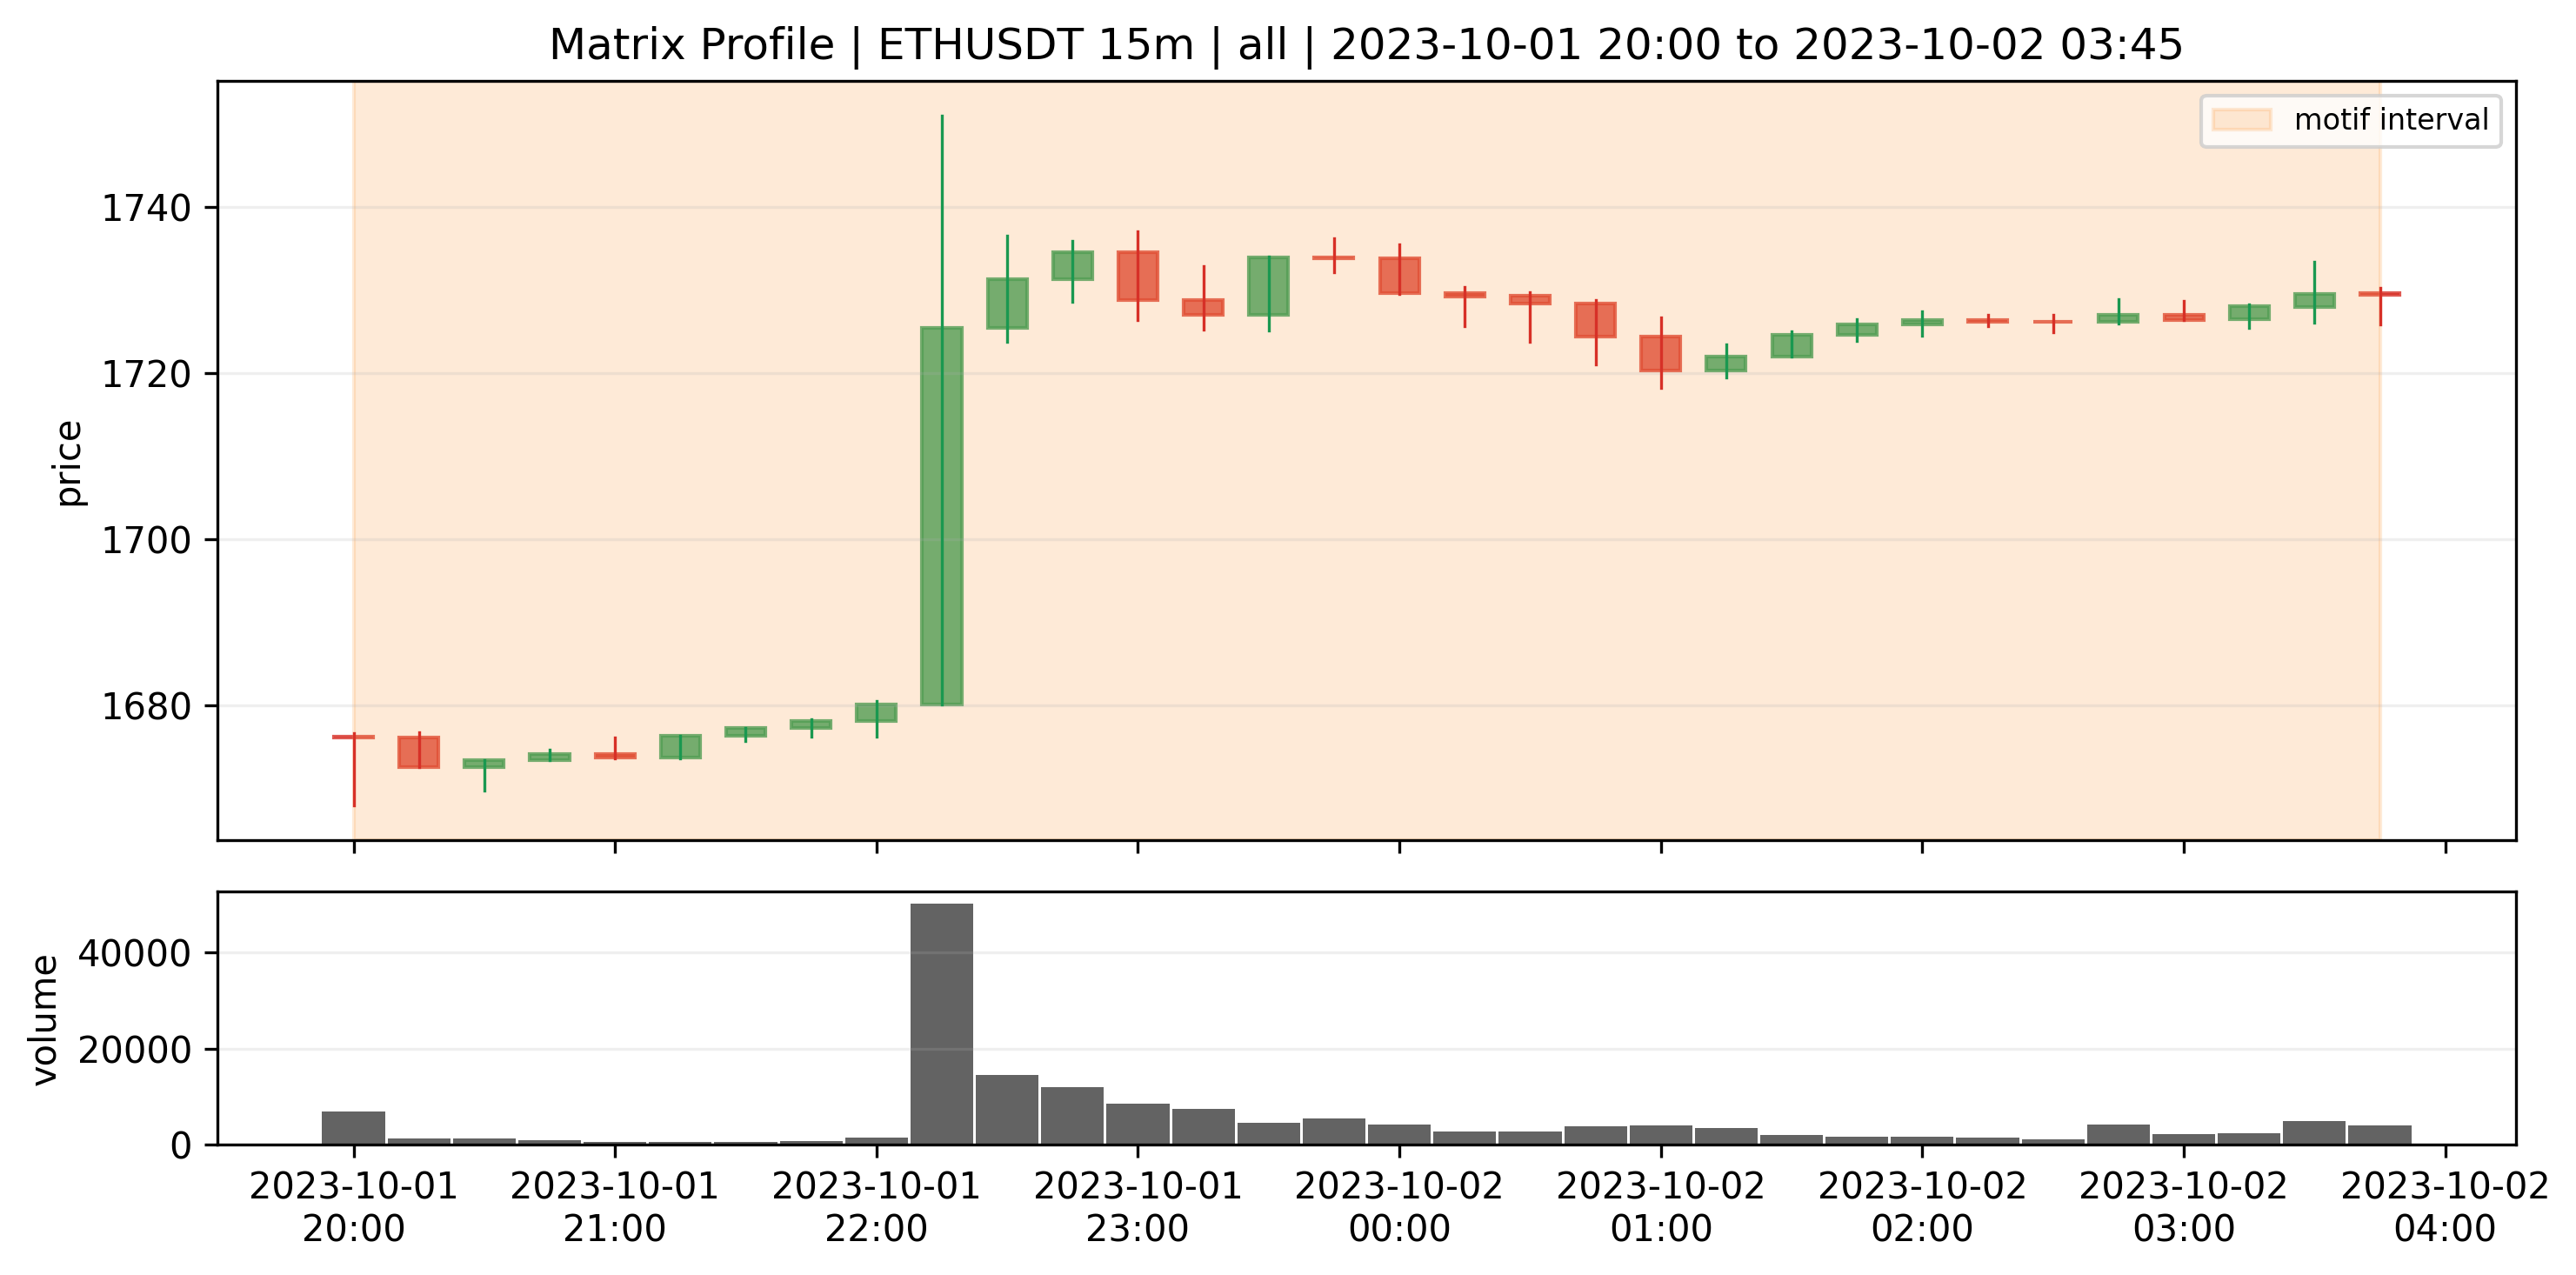
\includegraphics[width=0.9\linewidth]{reports/final_visual_evidence/figures/top_motif_04_matrix_profile_ethusdt_15m_all_zoom.png}
\caption{top motif 04 matrix profile ethusdt 15m all zoom. The shaded interval marks the discovered motif occurrence in original price context.}
\end{figure}

\begin{figure}[ht]
\centering
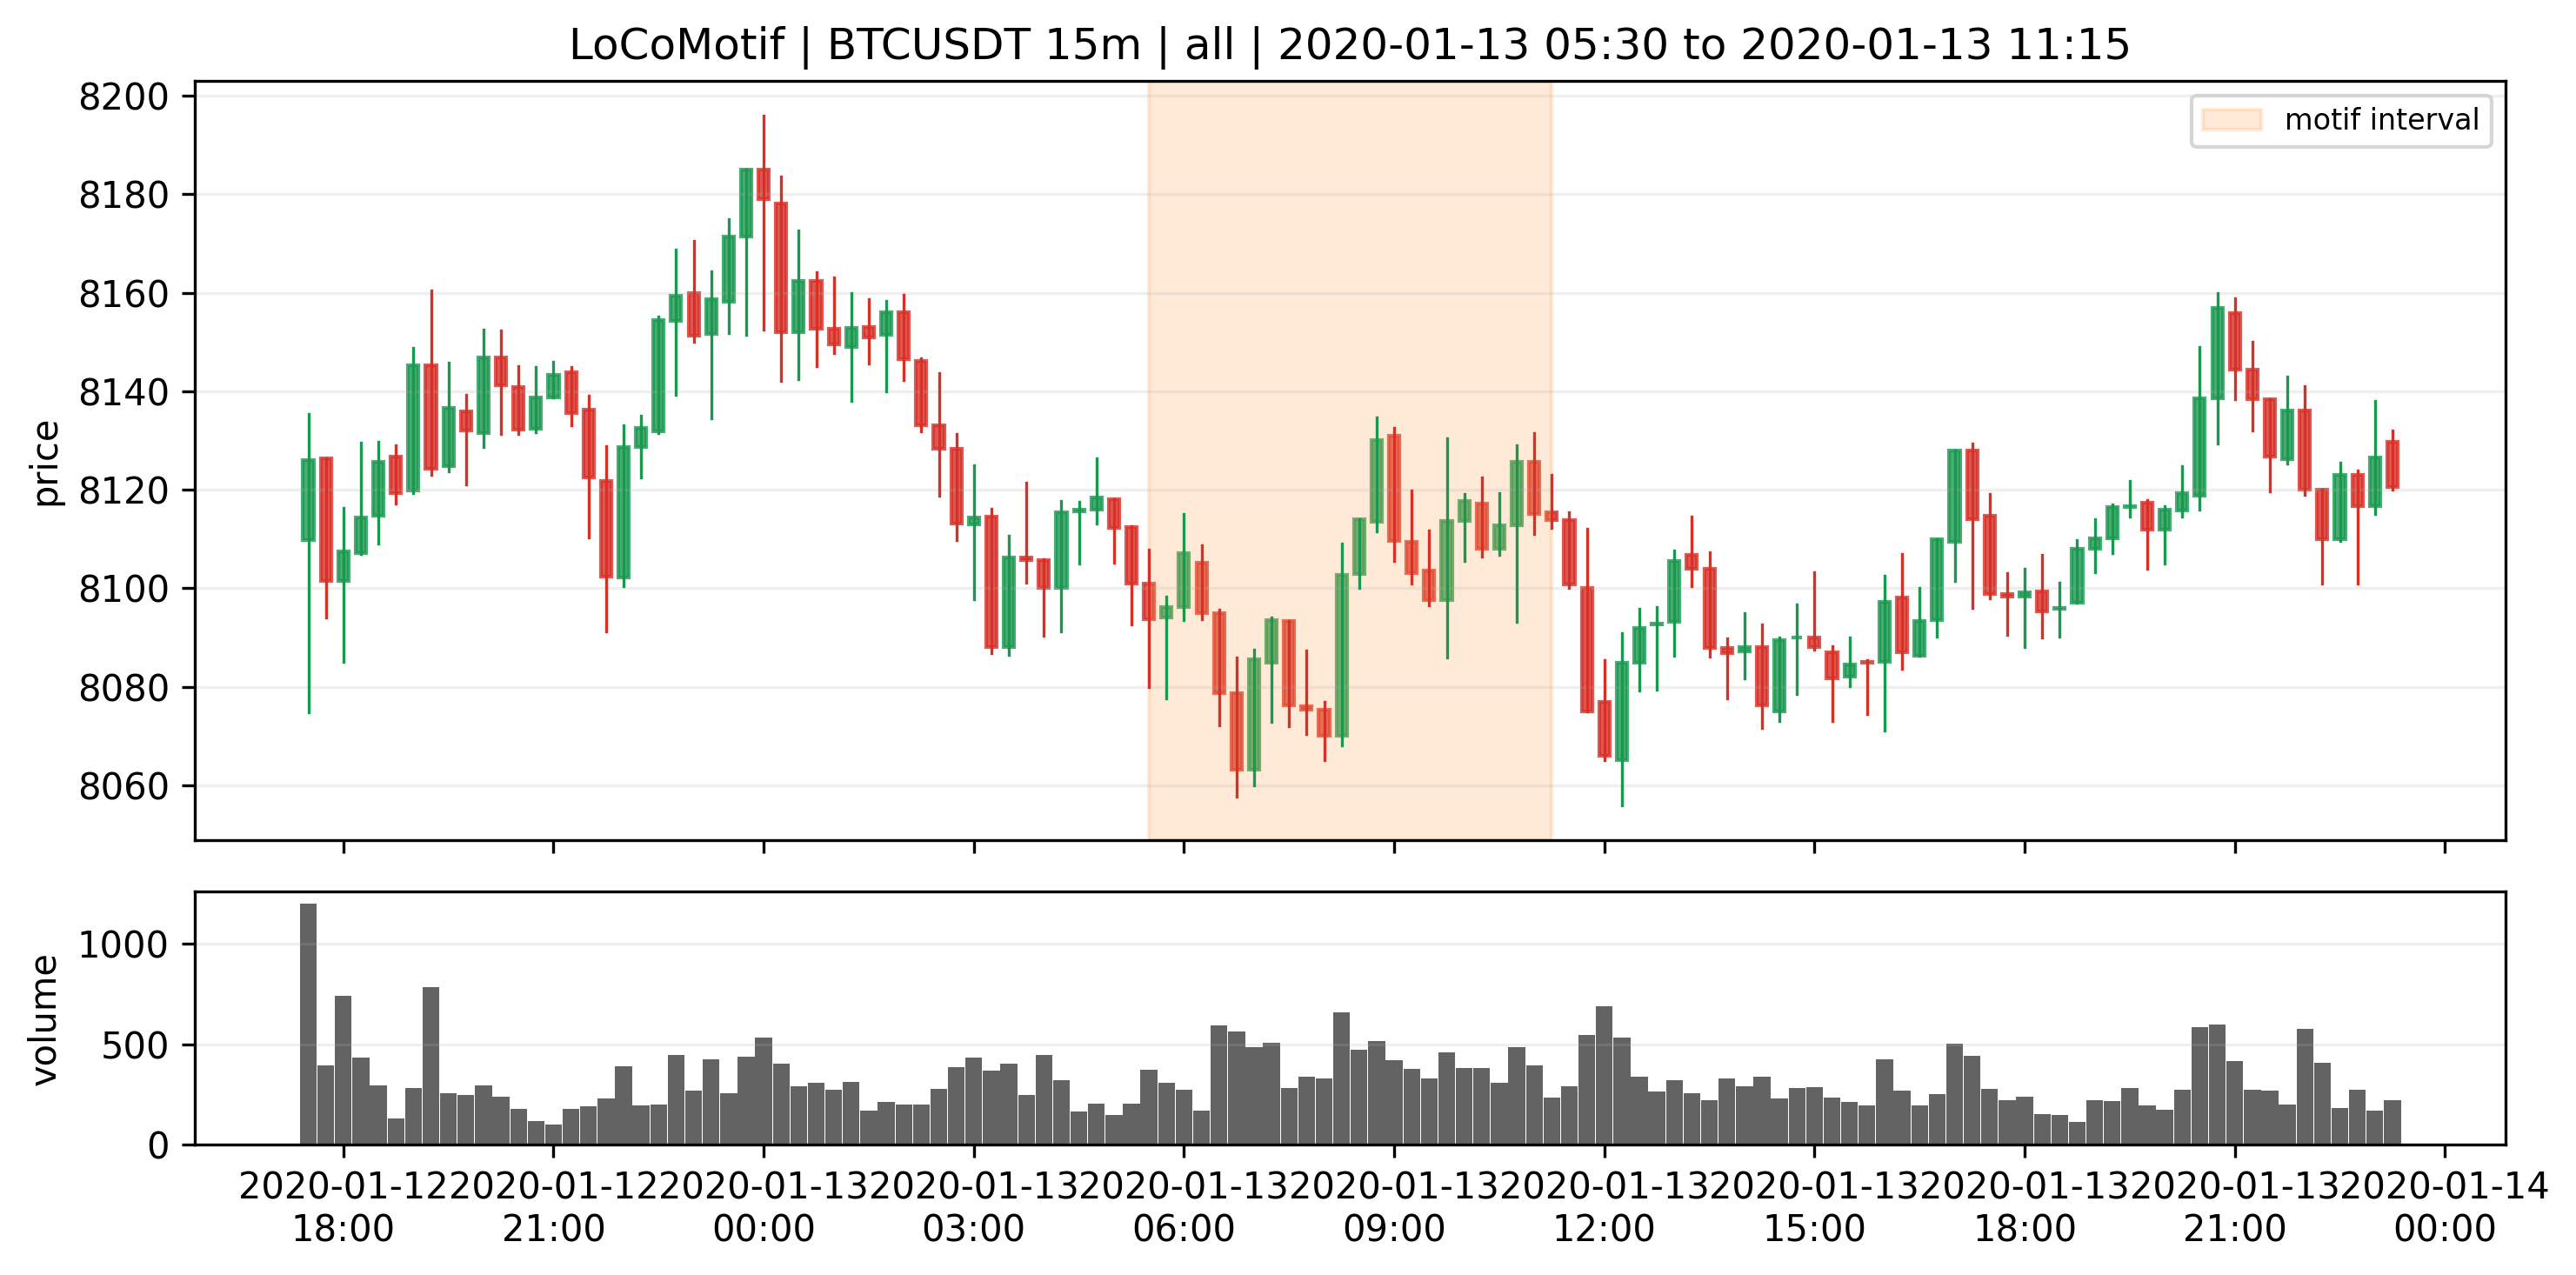
\includegraphics[width=0.9\linewidth]{reports/final_visual_evidence/figures/top_motif_05_locomotif_btcusdt_15m_all_context.png}
\caption{top motif 05 locomotif btcusdt 15m all context. The figure compares real available Matrix Profile and LoCoMotif outputs while preserving object-type differences.}
\end{figure}

\begin{figure}[ht]
\centering
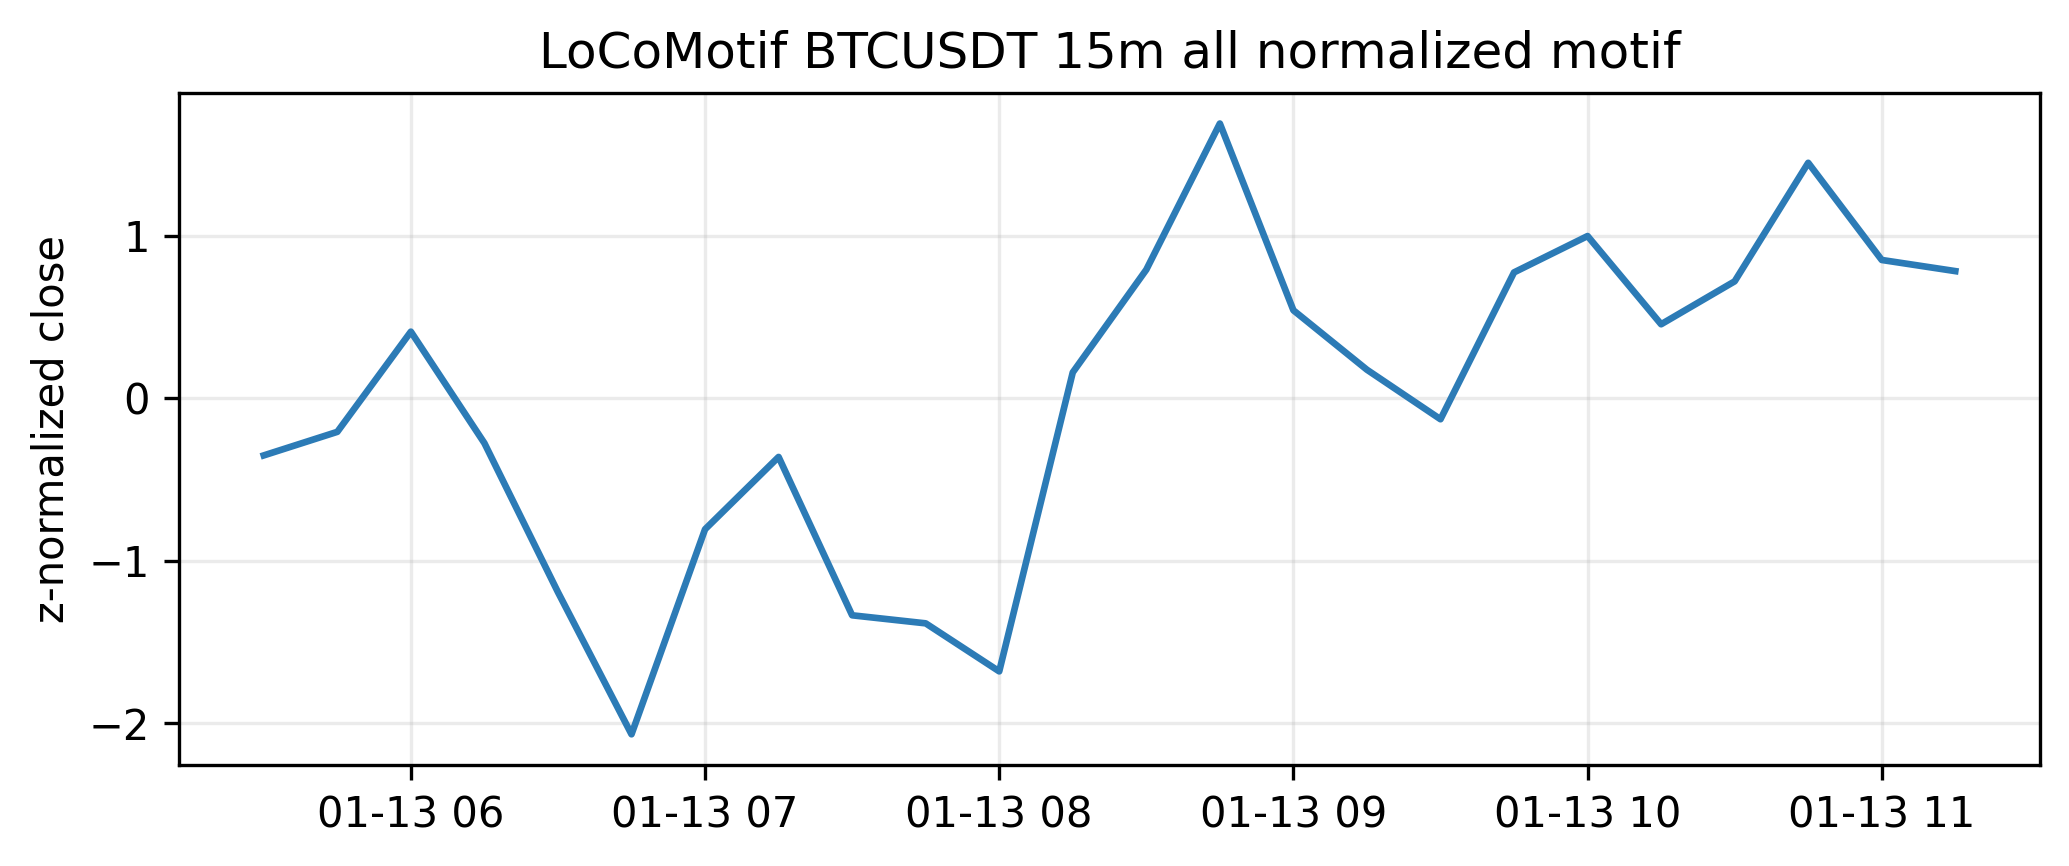
\includegraphics[width=0.9\linewidth]{reports/final_visual_evidence/figures/top_motif_05_locomotif_btcusdt_15m_all_normal_pattern.png}
\caption{top motif 05 locomotif btcusdt 15m all normal pattern. The figure compares real available Matrix Profile and LoCoMotif outputs while preserving object-type differences.}
\end{figure}

\begin{figure}[ht]
\centering
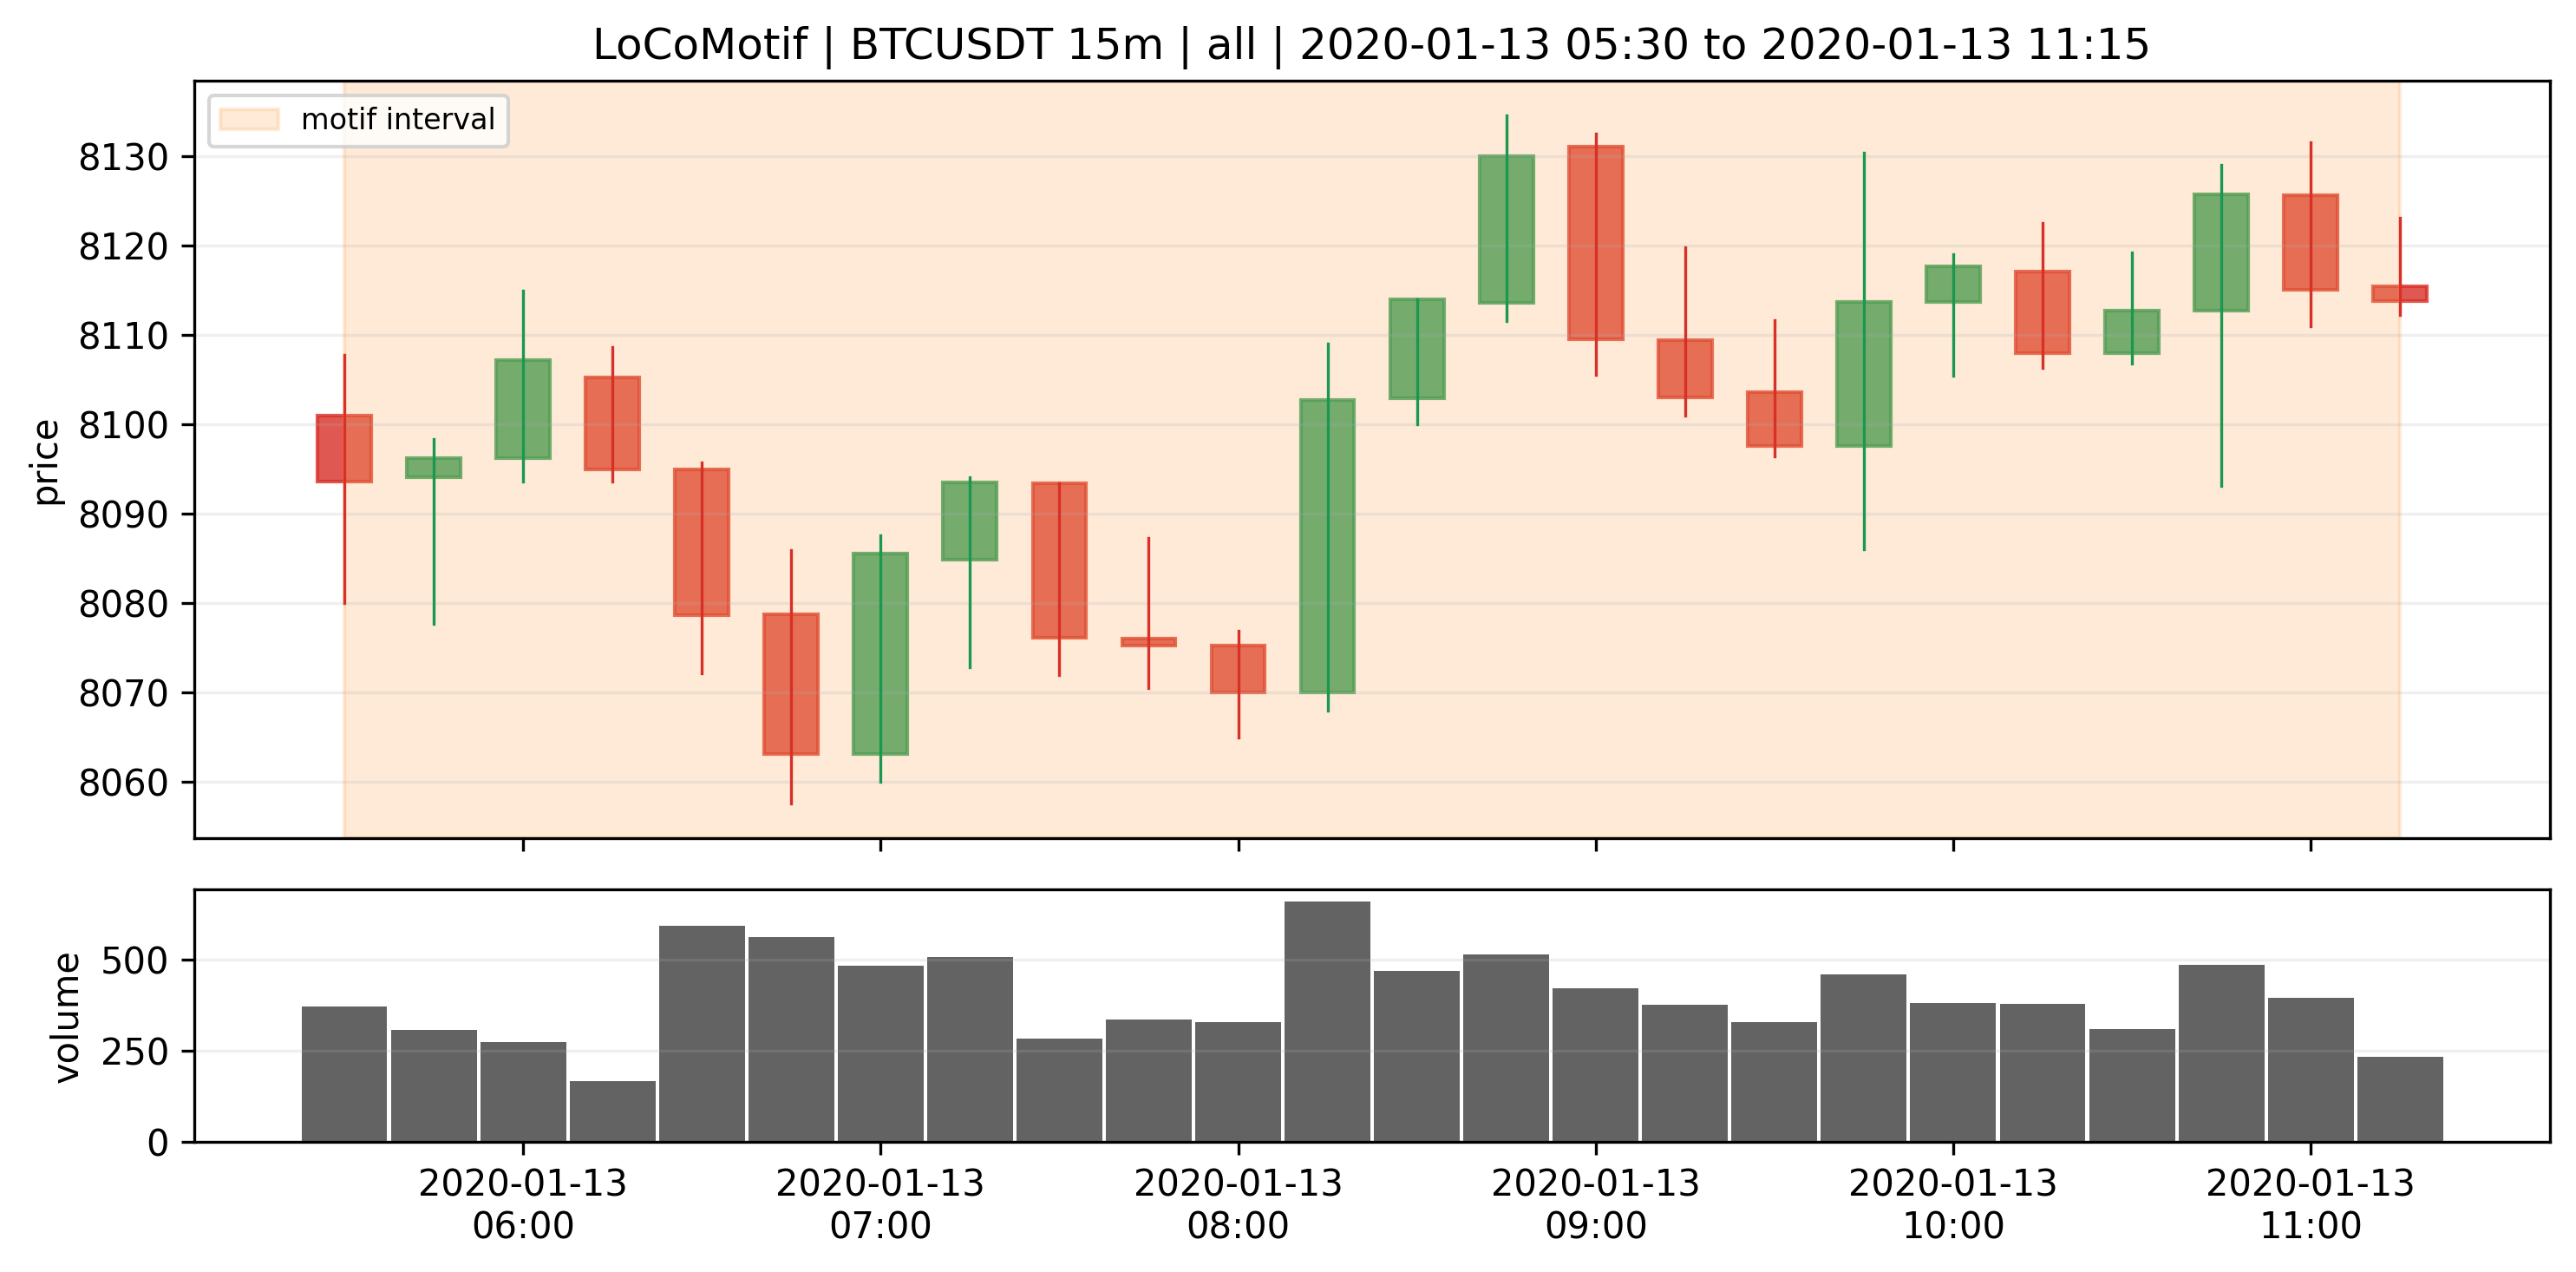
\includegraphics[width=0.9\linewidth]{reports/final_visual_evidence/figures/top_motif_05_locomotif_btcusdt_15m_all_zoom.png}
\caption{top motif 05 locomotif btcusdt 15m all zoom. The figure compares real available Matrix Profile and LoCoMotif outputs while preserving object-type differences.}
\end{figure}

\begin{figure}[ht]
\centering
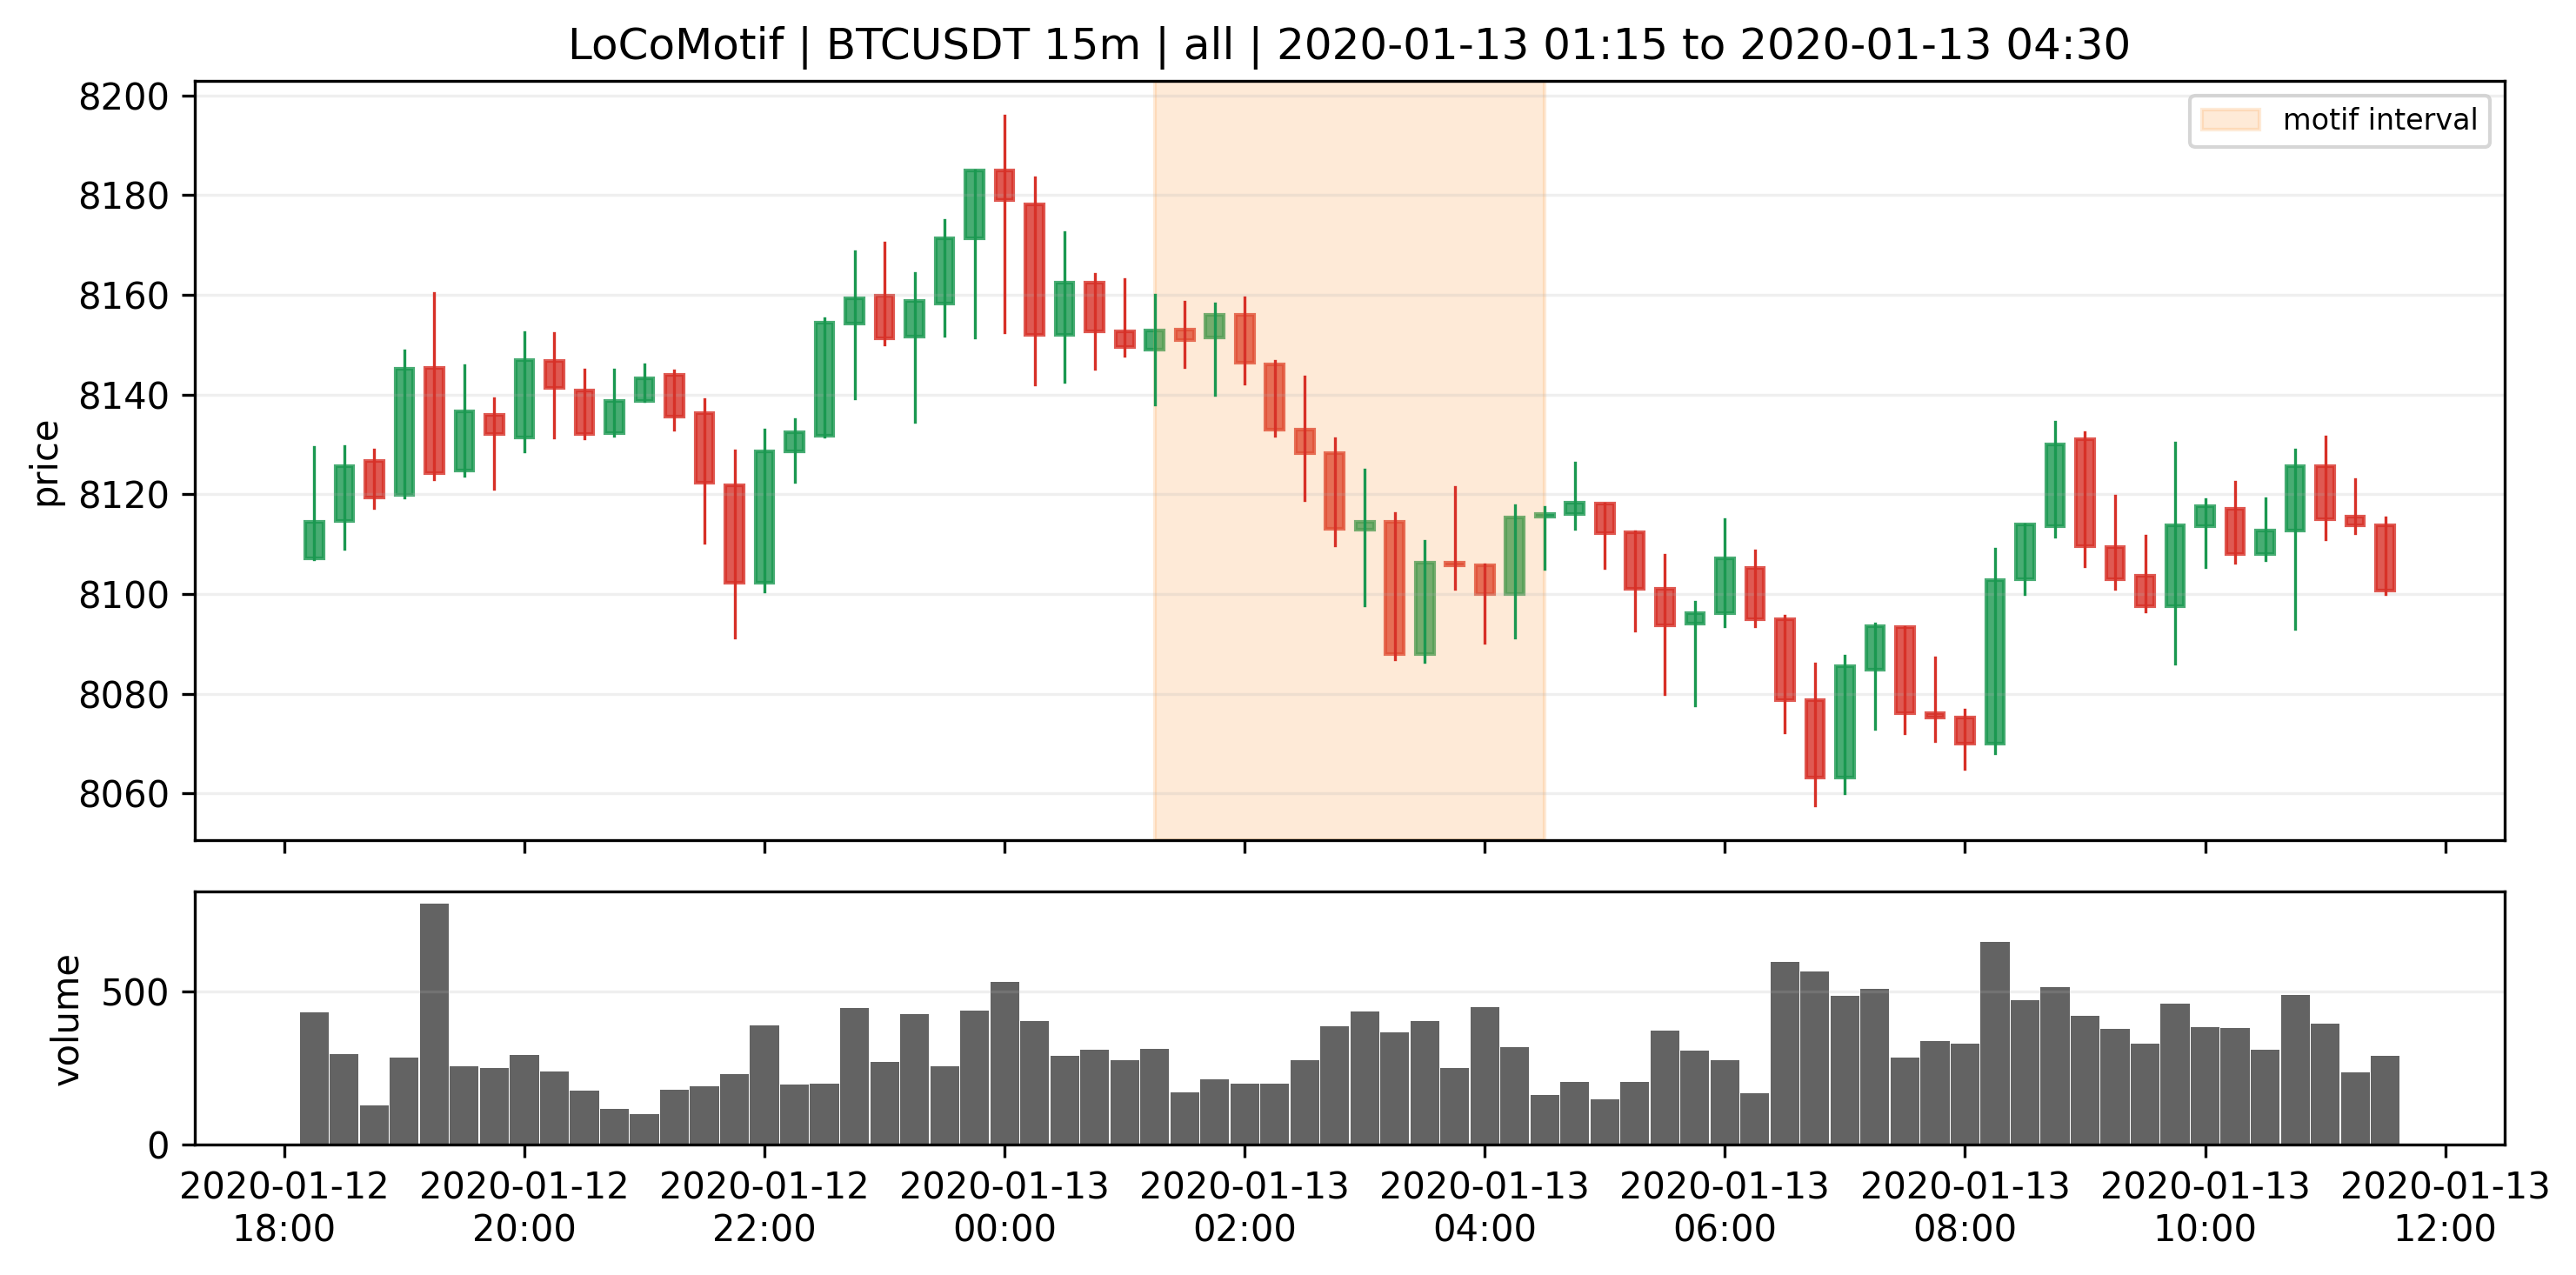
\includegraphics[width=0.9\linewidth]{reports/final_visual_evidence/figures/top_motif_06_locomotif_btcusdt_15m_all_context.png}
\caption{top motif 06 locomotif btcusdt 15m all context. The figure compares real available Matrix Profile and LoCoMotif outputs while preserving object-type differences.}
\end{figure}

\begin{figure}[ht]
\centering
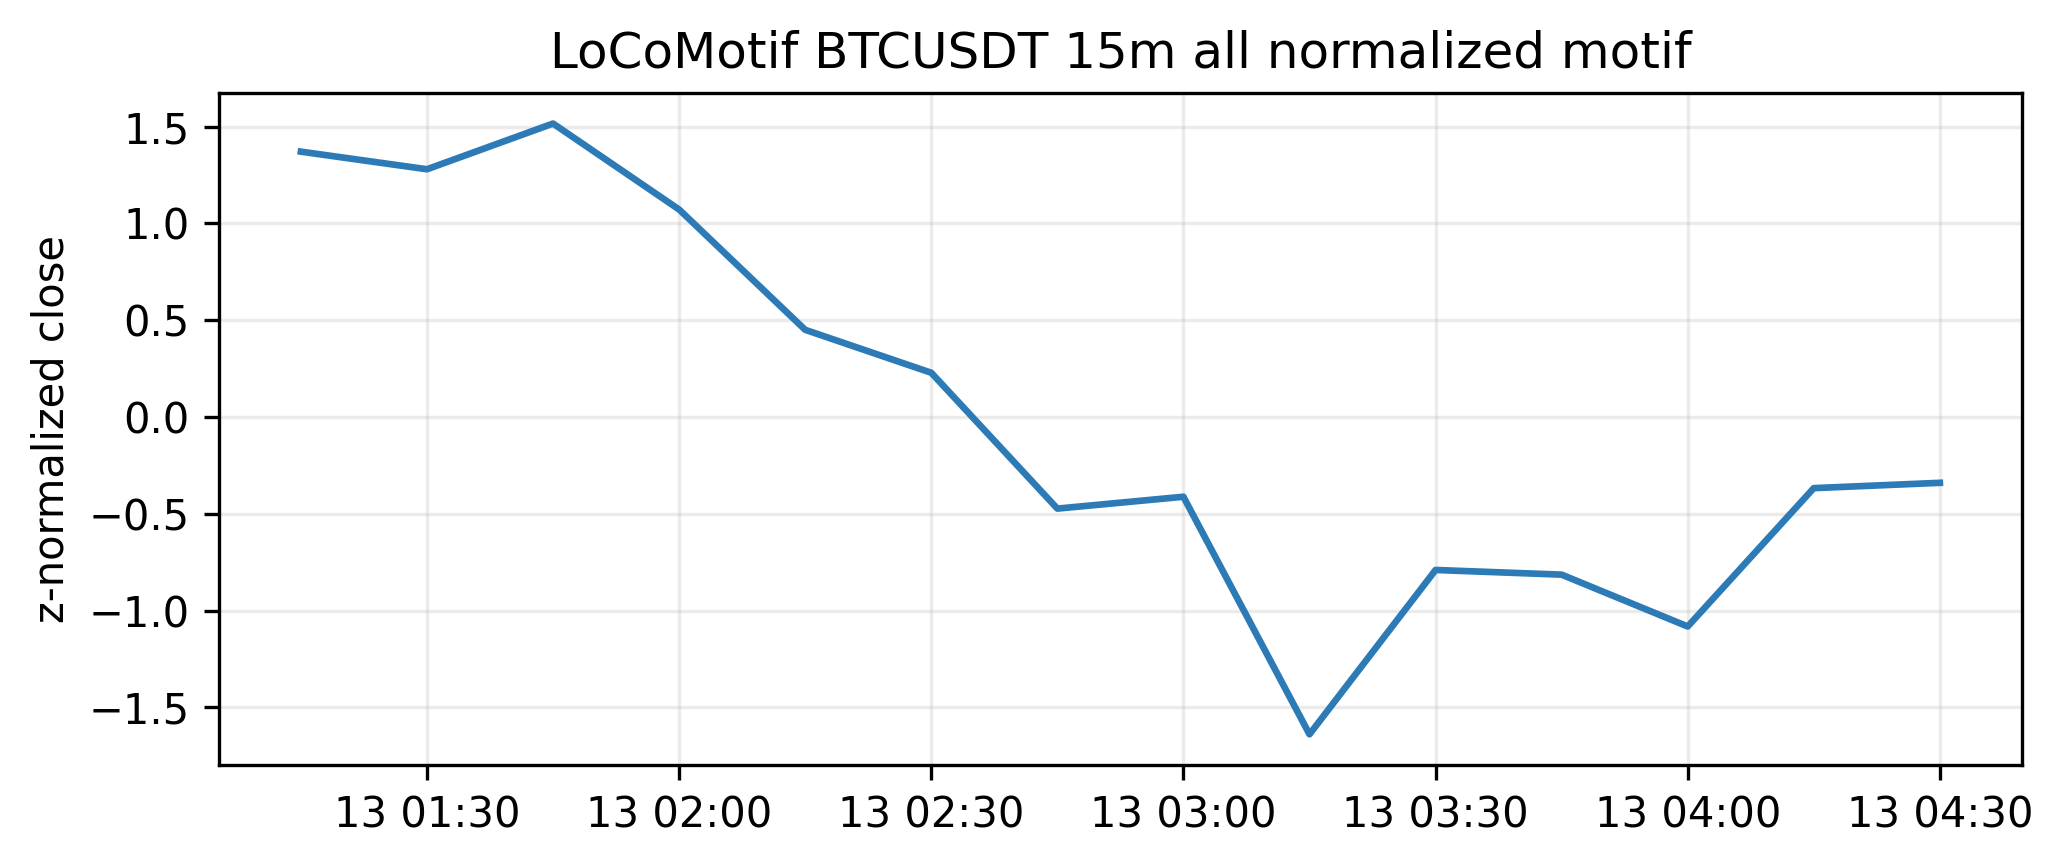
\includegraphics[width=0.9\linewidth]{reports/final_visual_evidence/figures/top_motif_06_locomotif_btcusdt_15m_all_normal_pattern.png}
\caption{top motif 06 locomotif btcusdt 15m all normal pattern. The figure compares real available Matrix Profile and LoCoMotif outputs while preserving object-type differences.}
\end{figure}

\begin{figure}[ht]
\centering
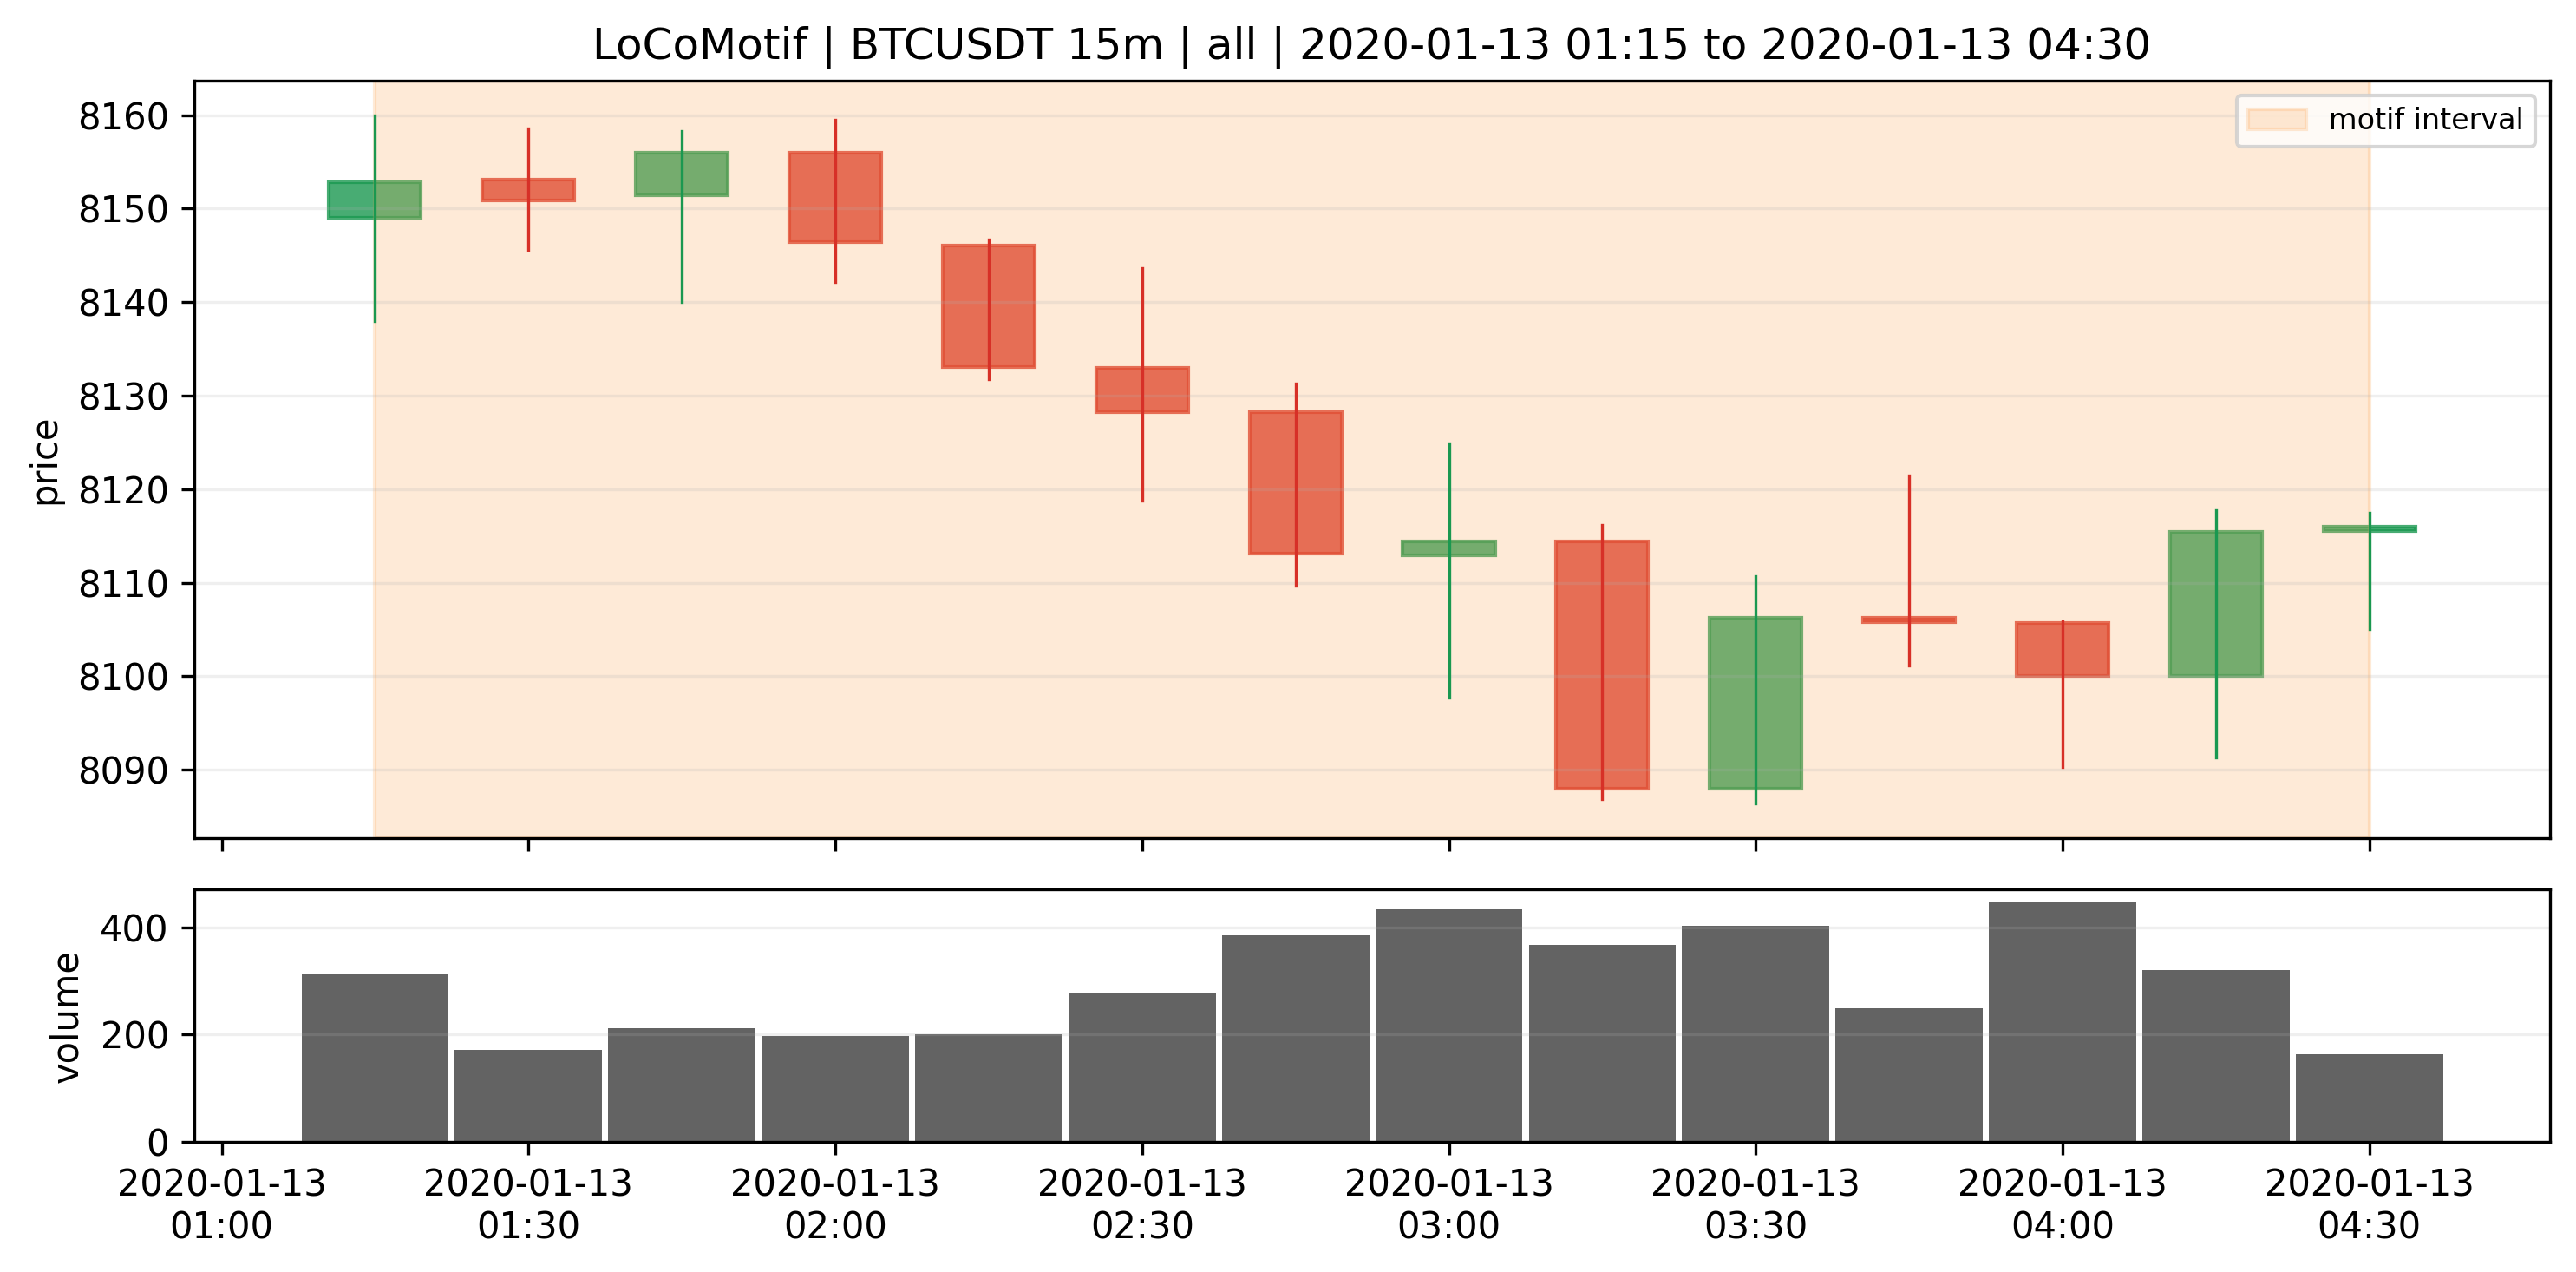
\includegraphics[width=0.9\linewidth]{reports/final_visual_evidence/figures/top_motif_06_locomotif_btcusdt_15m_all_zoom.png}
\caption{top motif 06 locomotif btcusdt 15m all zoom. The figure compares real available Matrix Profile and LoCoMotif outputs while preserving object-type differences.}
\end{figure}

\begin{figure}[ht]
\centering
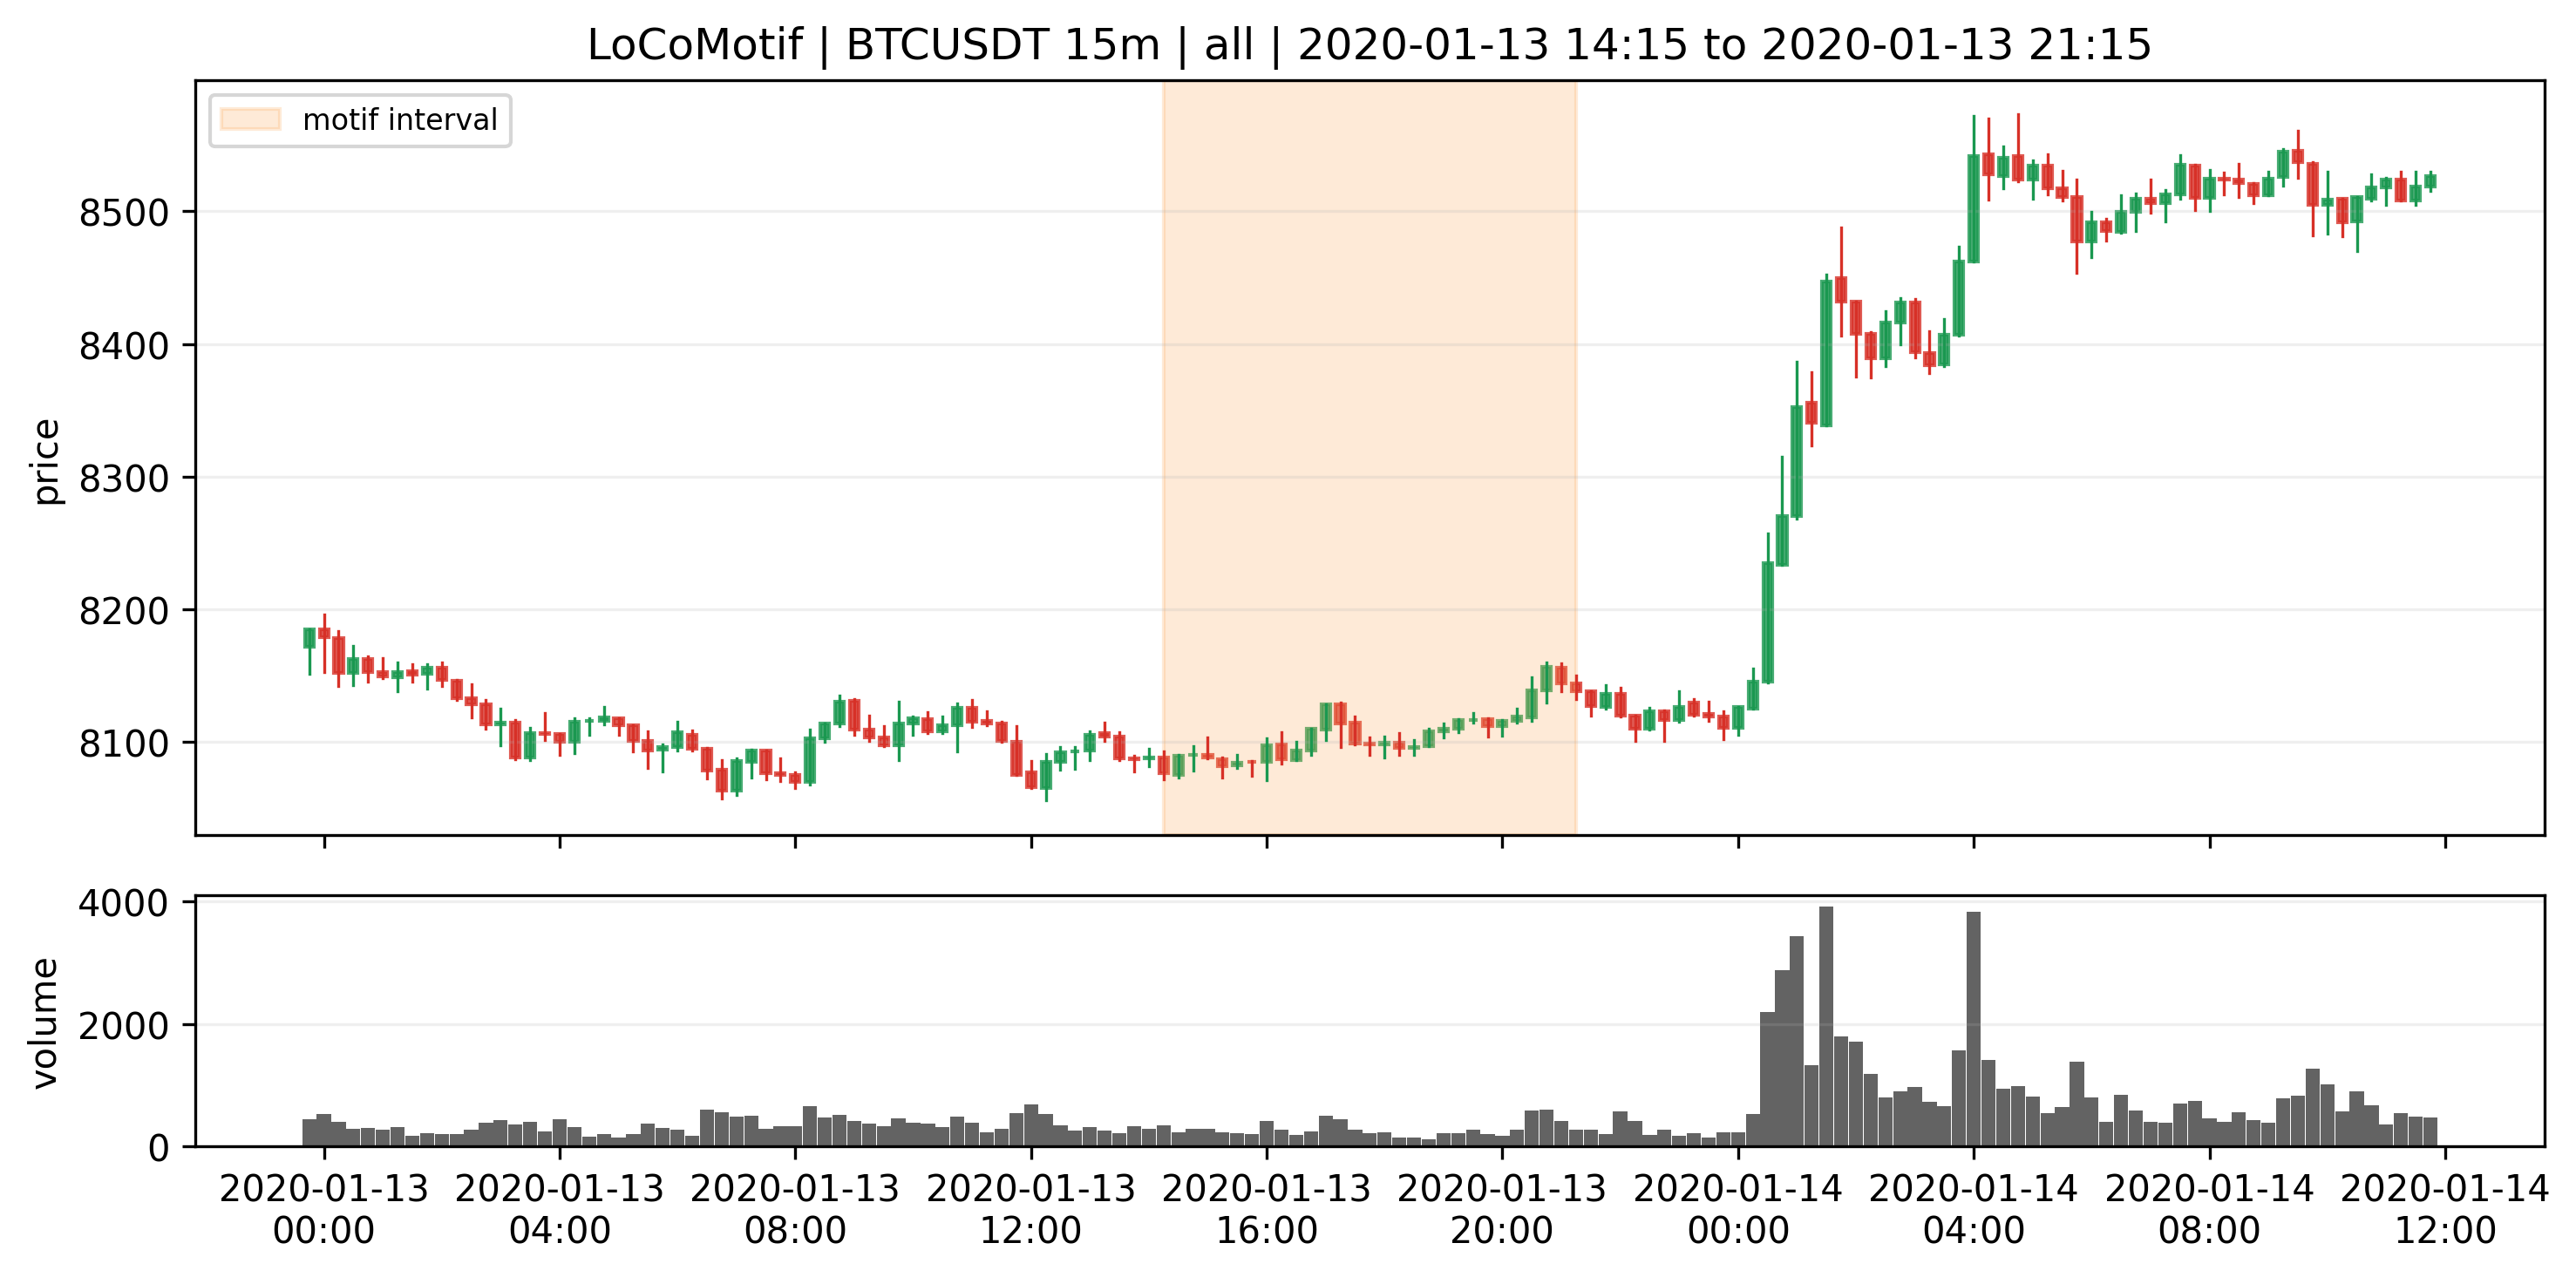
\includegraphics[width=0.9\linewidth]{reports/final_visual_evidence/figures/top_motif_07_locomotif_btcusdt_15m_all_context.png}
\caption{top motif 07 locomotif btcusdt 15m all context. The figure compares real available Matrix Profile and LoCoMotif outputs while preserving object-type differences.}
\end{figure}

\begin{figure}[ht]
\centering
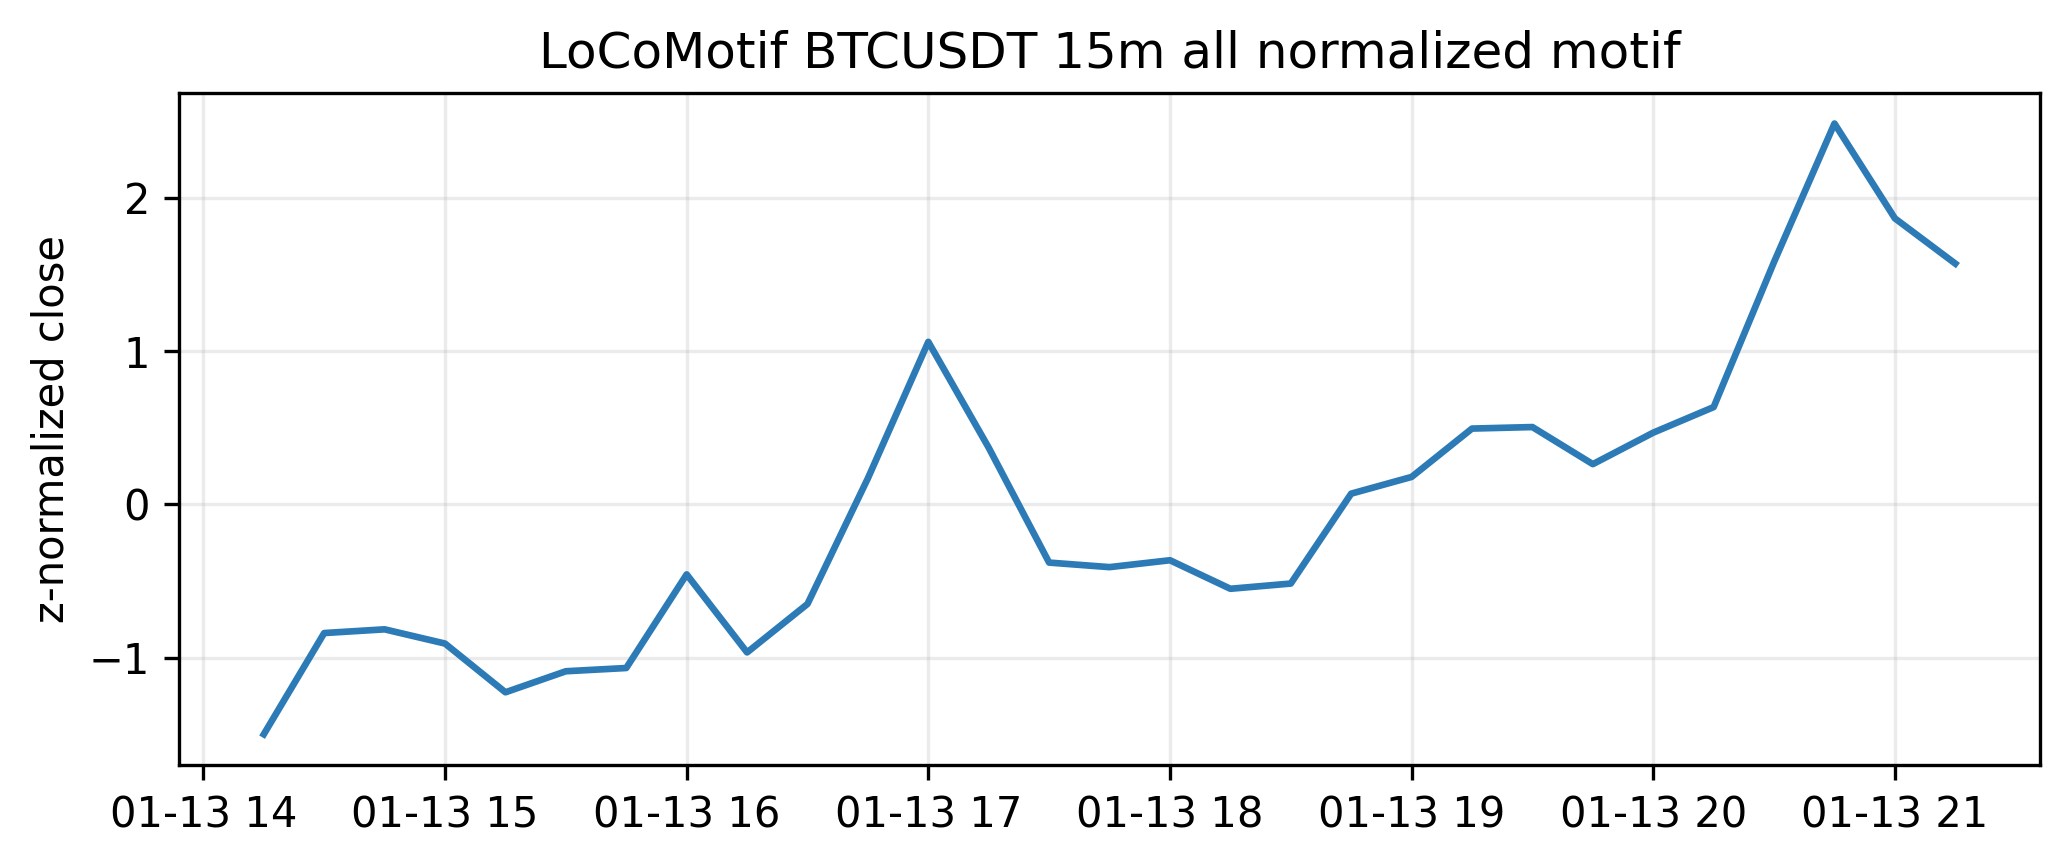
\includegraphics[width=0.9\linewidth]{reports/final_visual_evidence/figures/top_motif_07_locomotif_btcusdt_15m_all_normal_pattern.png}
\caption{top motif 07 locomotif btcusdt 15m all normal pattern. The figure compares real available Matrix Profile and LoCoMotif outputs while preserving object-type differences.}
\end{figure}

\begin{figure}[ht]
\centering
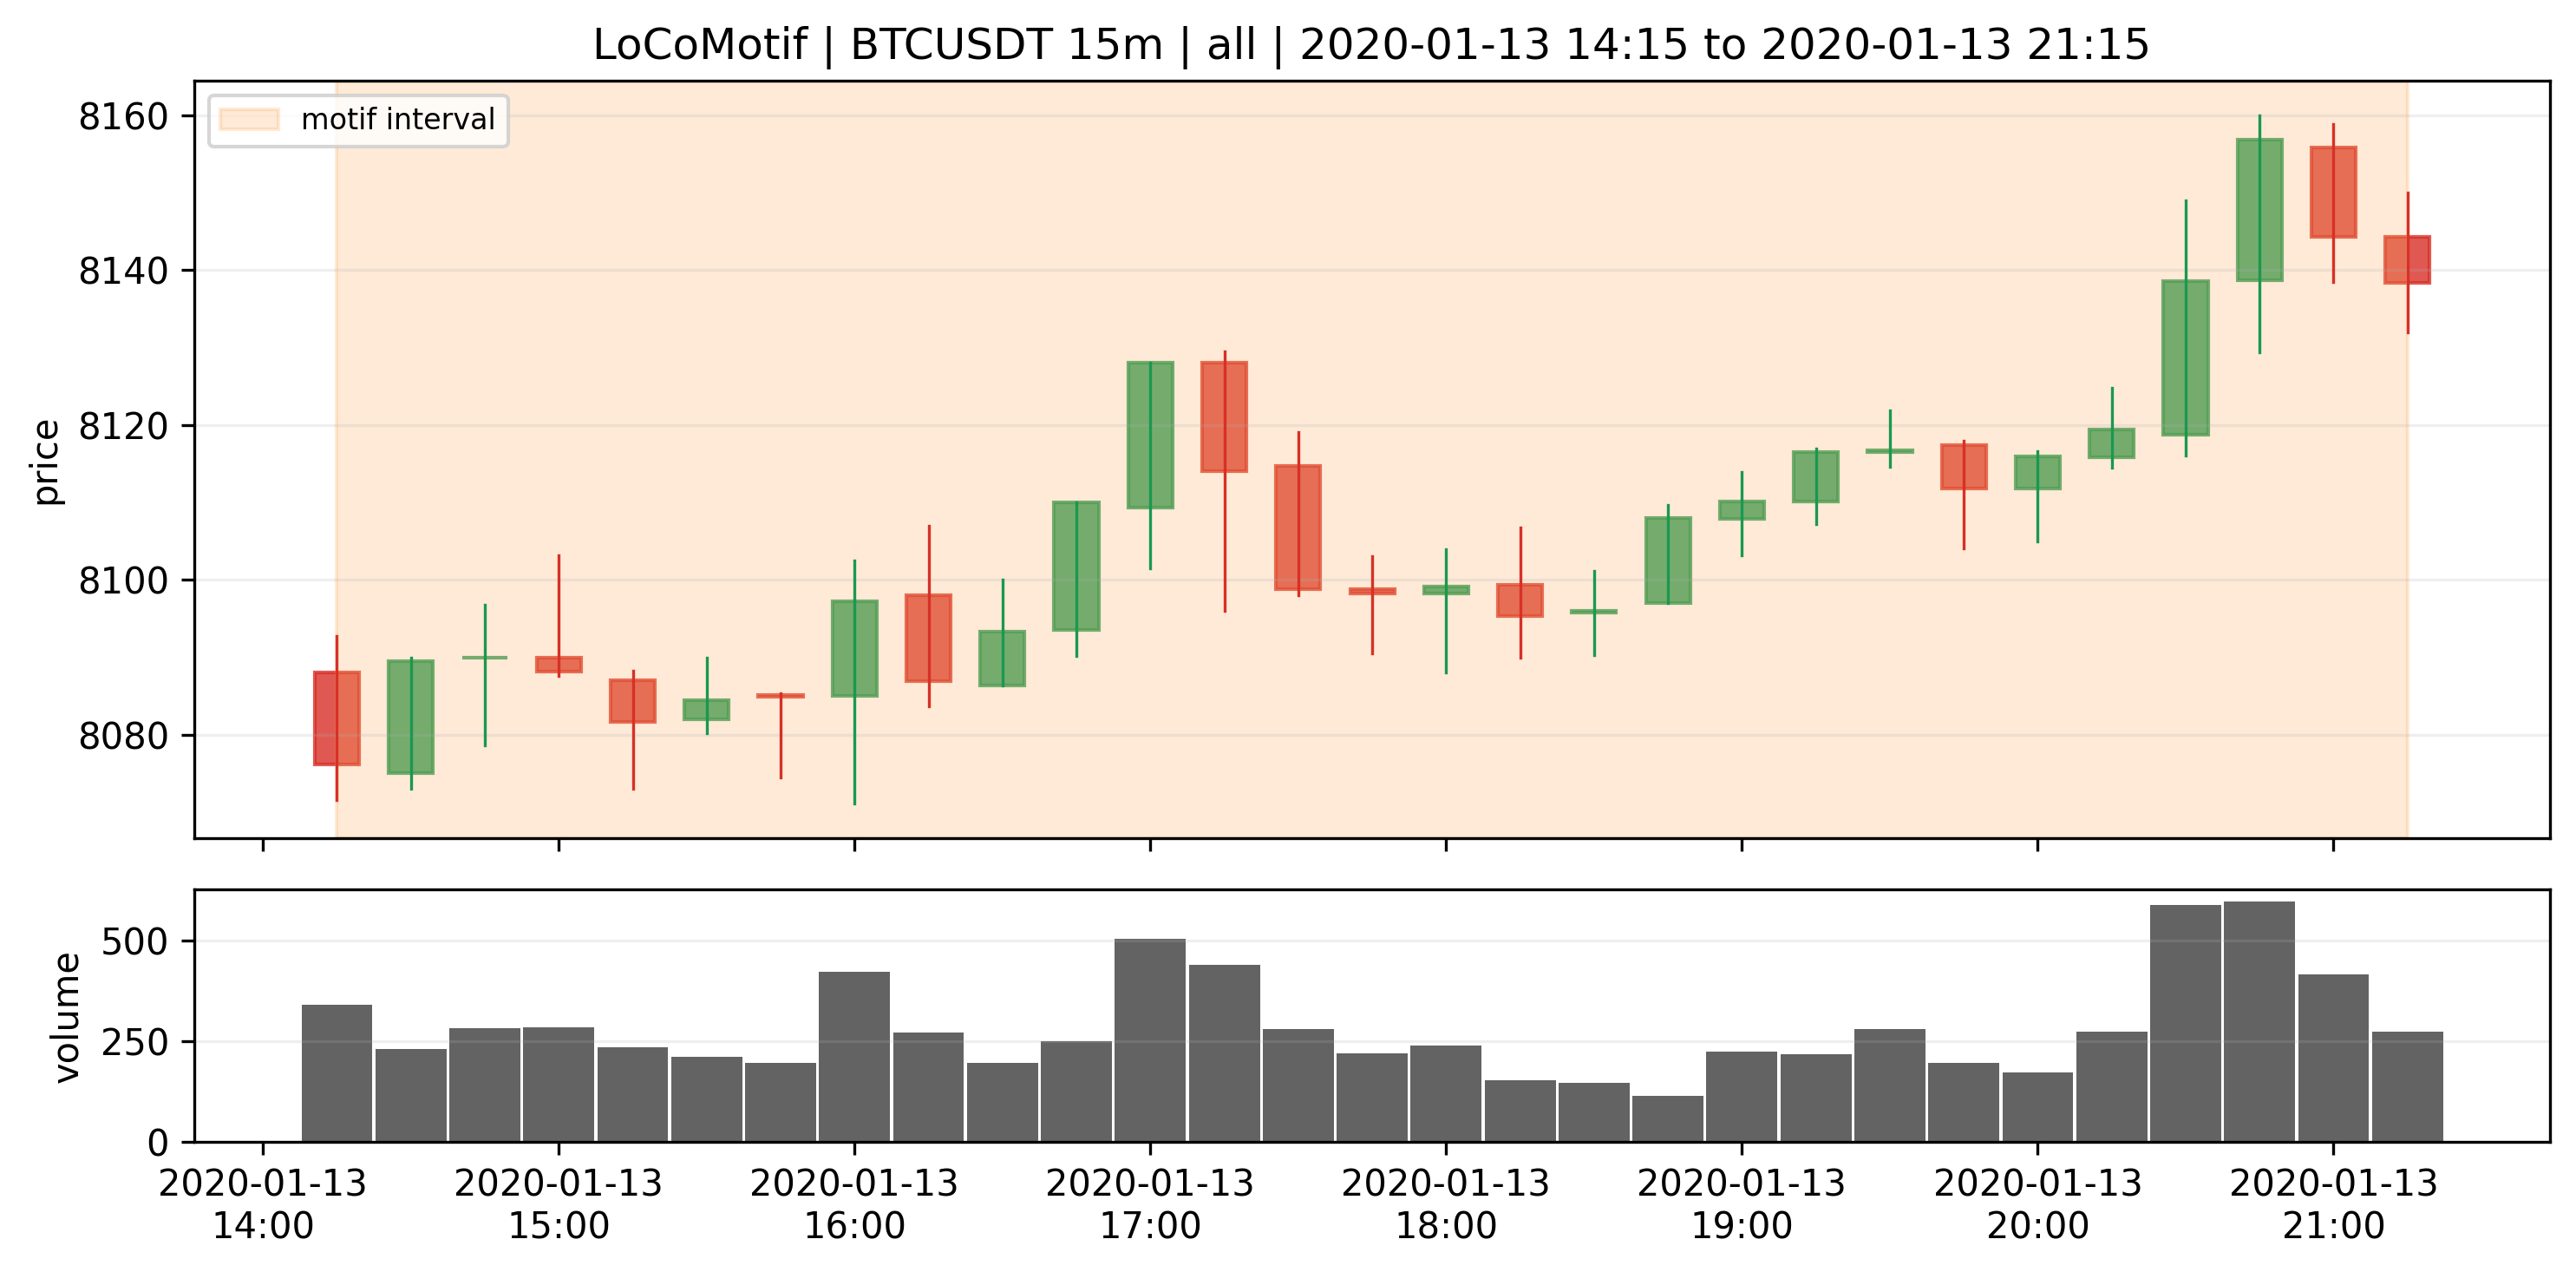
\includegraphics[width=0.9\linewidth]{reports/final_visual_evidence/figures/top_motif_07_locomotif_btcusdt_15m_all_zoom.png}
\caption{top motif 07 locomotif btcusdt 15m all zoom. The figure compares real available Matrix Profile and LoCoMotif outputs while preserving object-type differences.}
\end{figure}

\begin{figure}[ht]
\centering
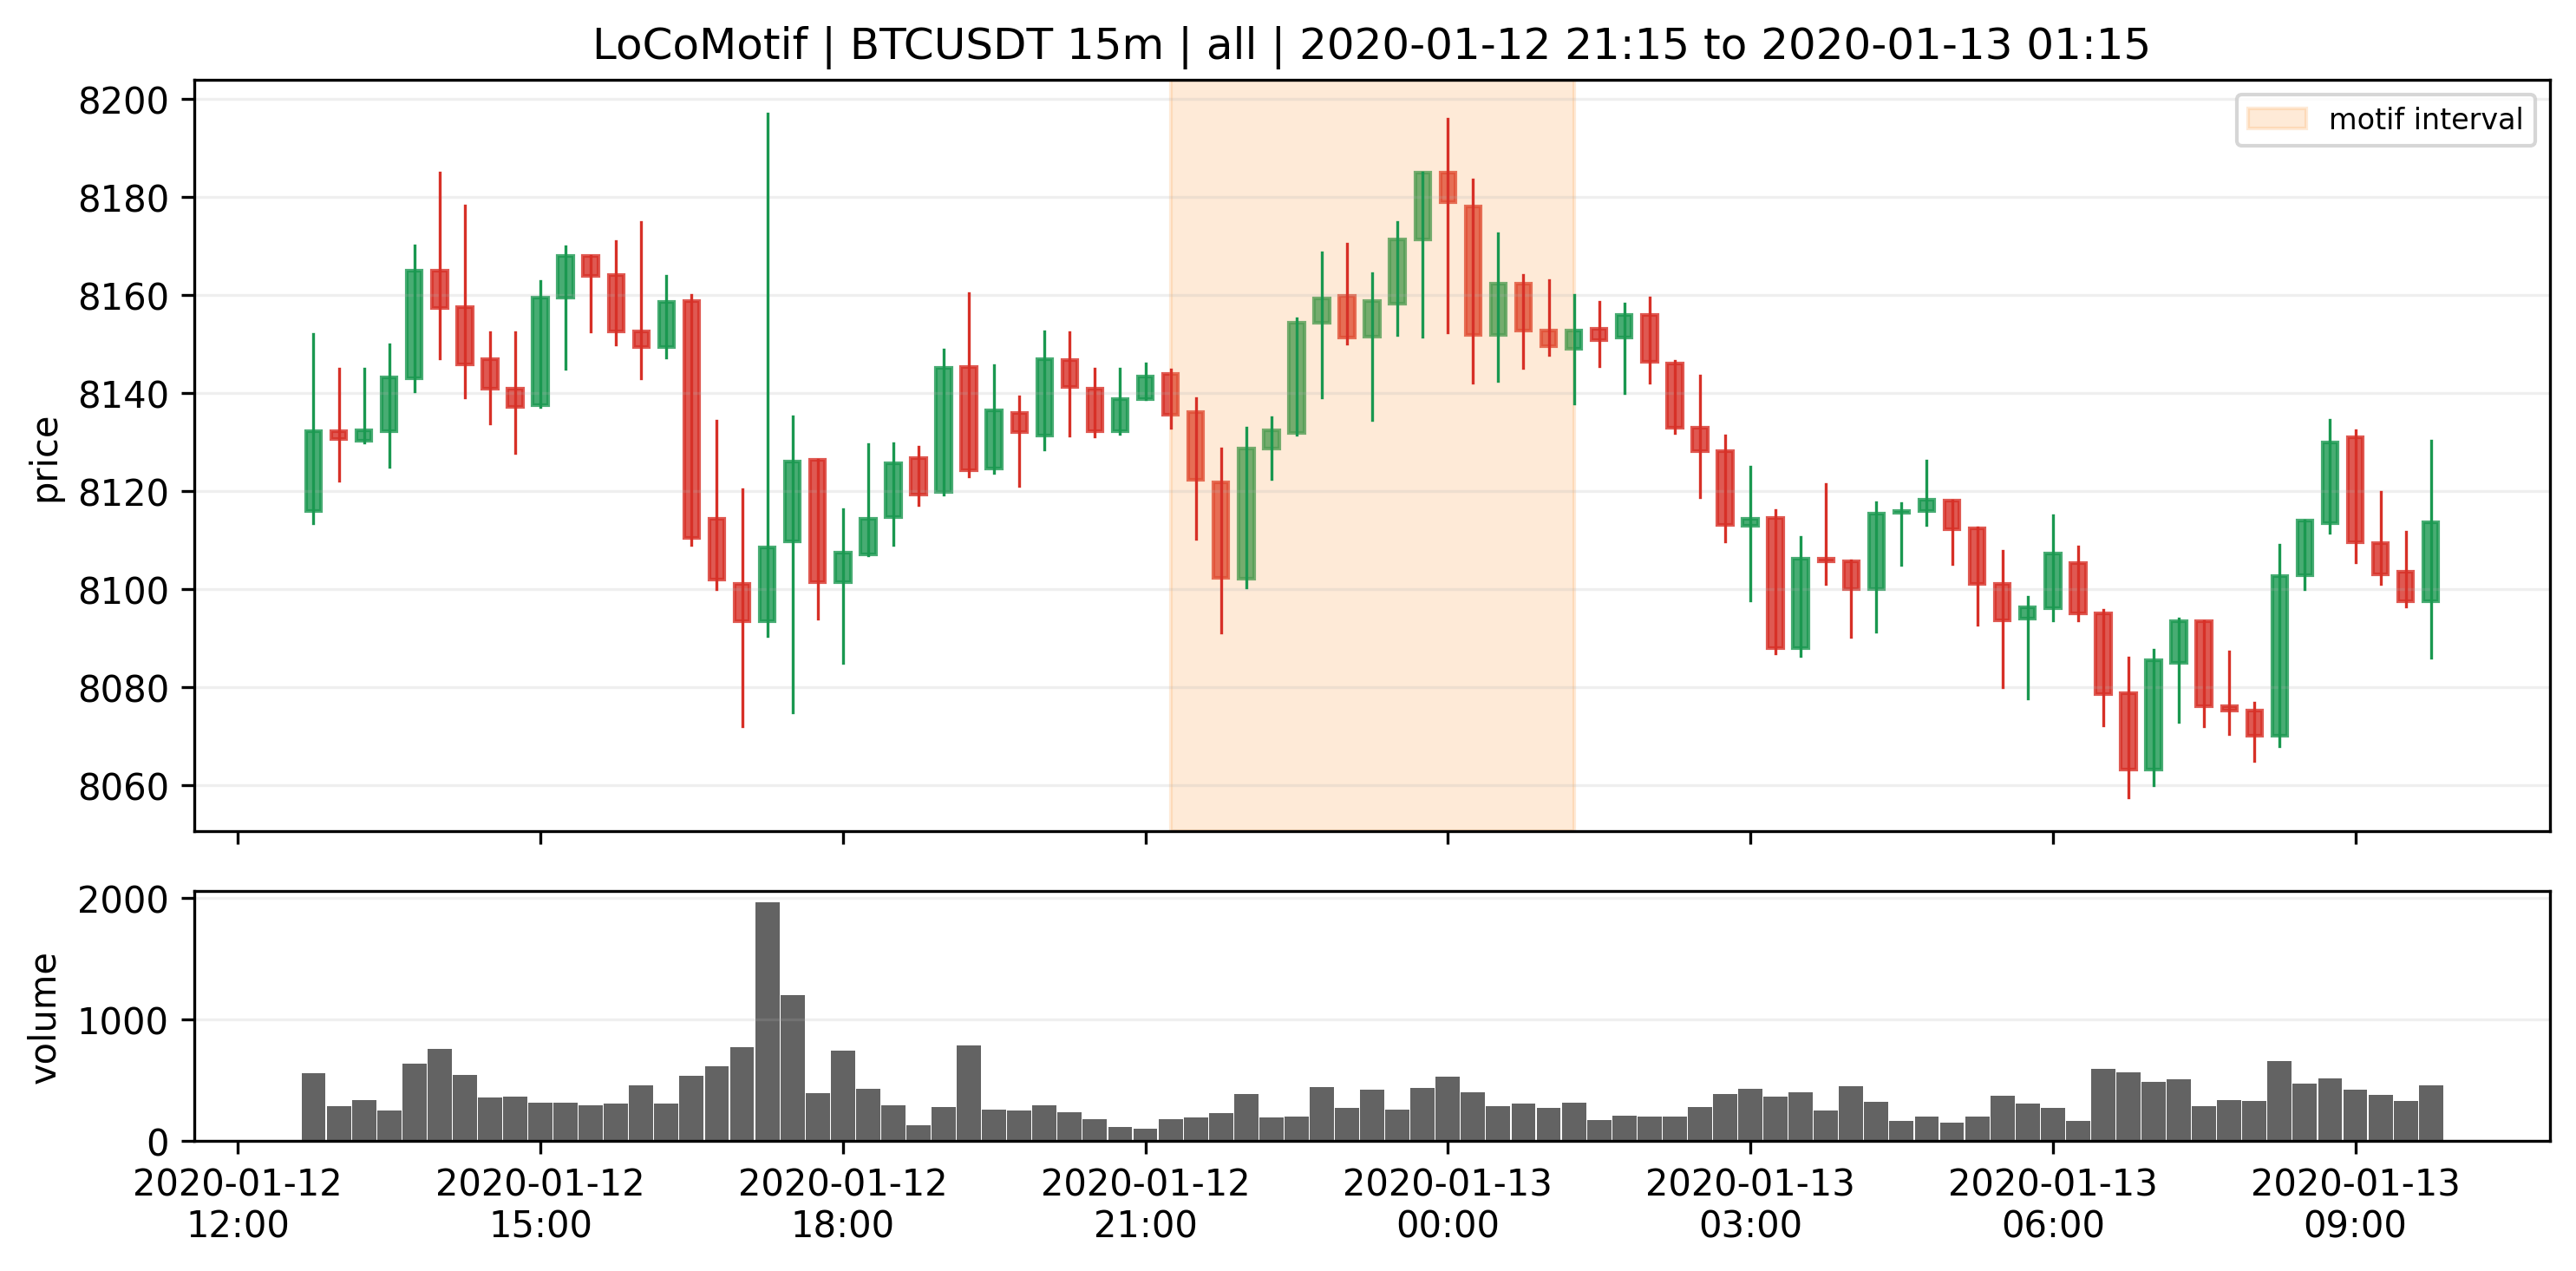
\includegraphics[width=0.9\linewidth]{reports/final_visual_evidence/figures/top_motif_08_locomotif_btcusdt_15m_all_context.png}
\caption{top motif 08 locomotif btcusdt 15m all context. The figure compares real available Matrix Profile and LoCoMotif outputs while preserving object-type differences.}
\end{figure}

\begin{figure}[ht]
\centering
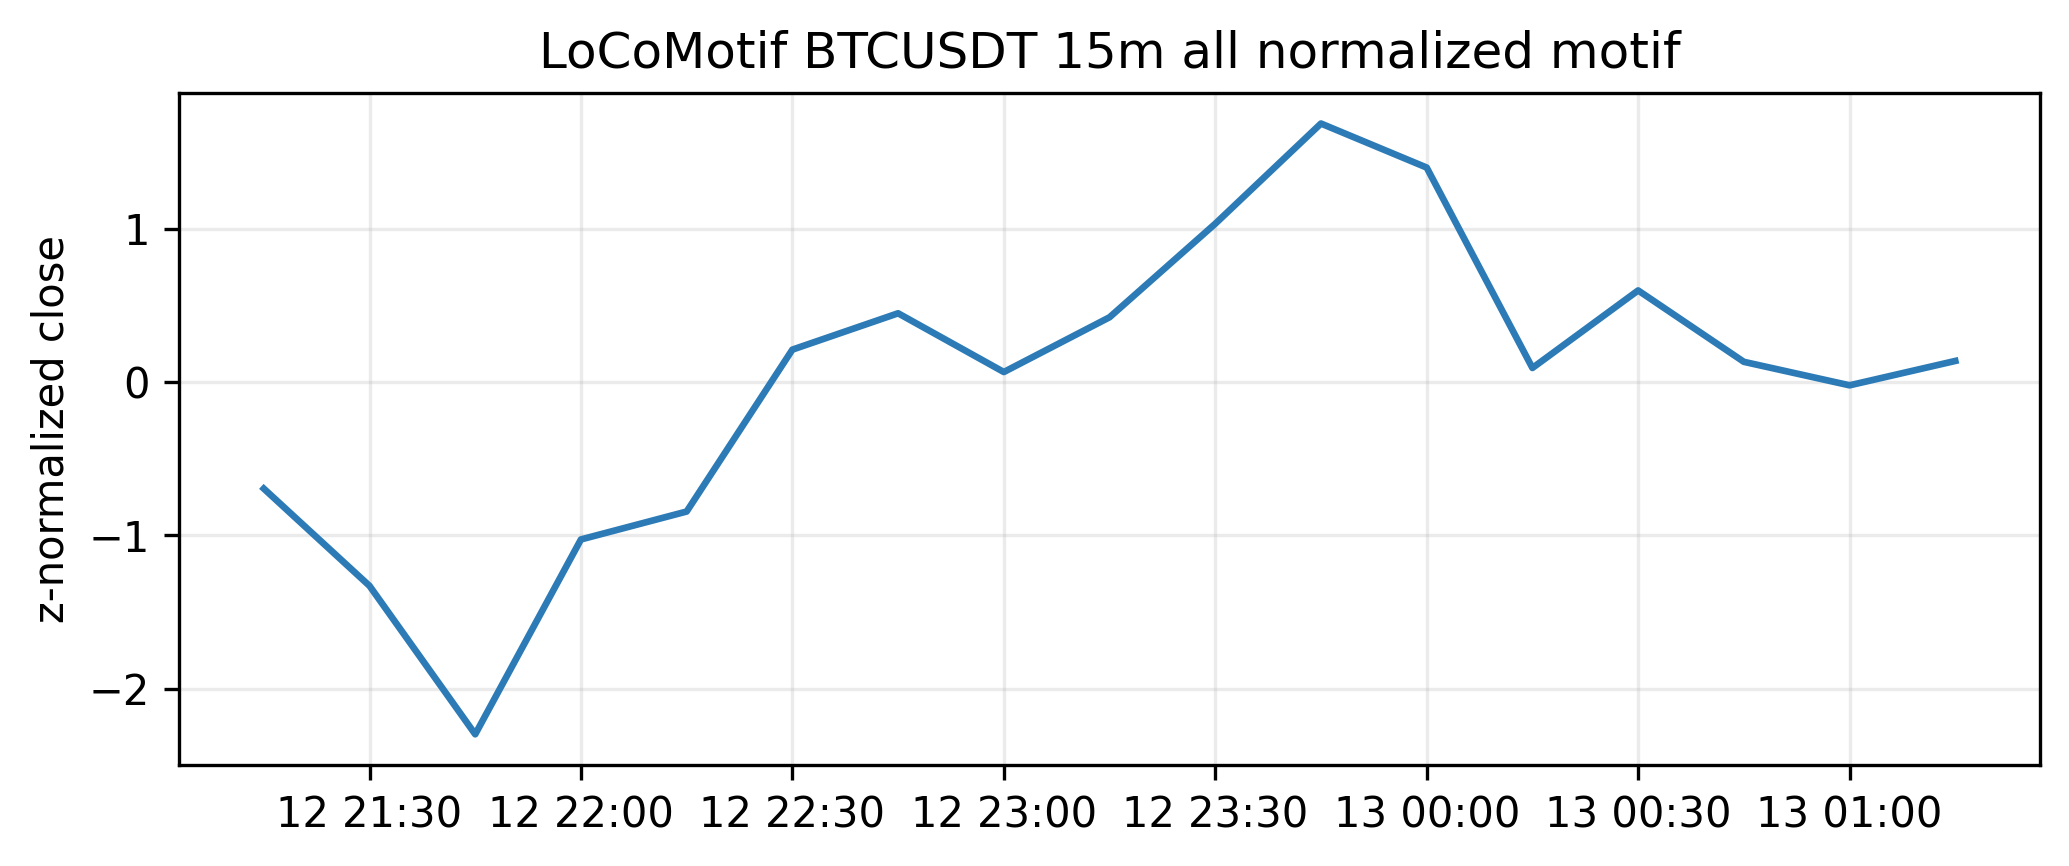
\includegraphics[width=0.9\linewidth]{reports/final_visual_evidence/figures/top_motif_08_locomotif_btcusdt_15m_all_normal_pattern.png}
\caption{top motif 08 locomotif btcusdt 15m all normal pattern. The figure compares real available Matrix Profile and LoCoMotif outputs while preserving object-type differences.}
\end{figure}

\begin{figure}[ht]
\centering
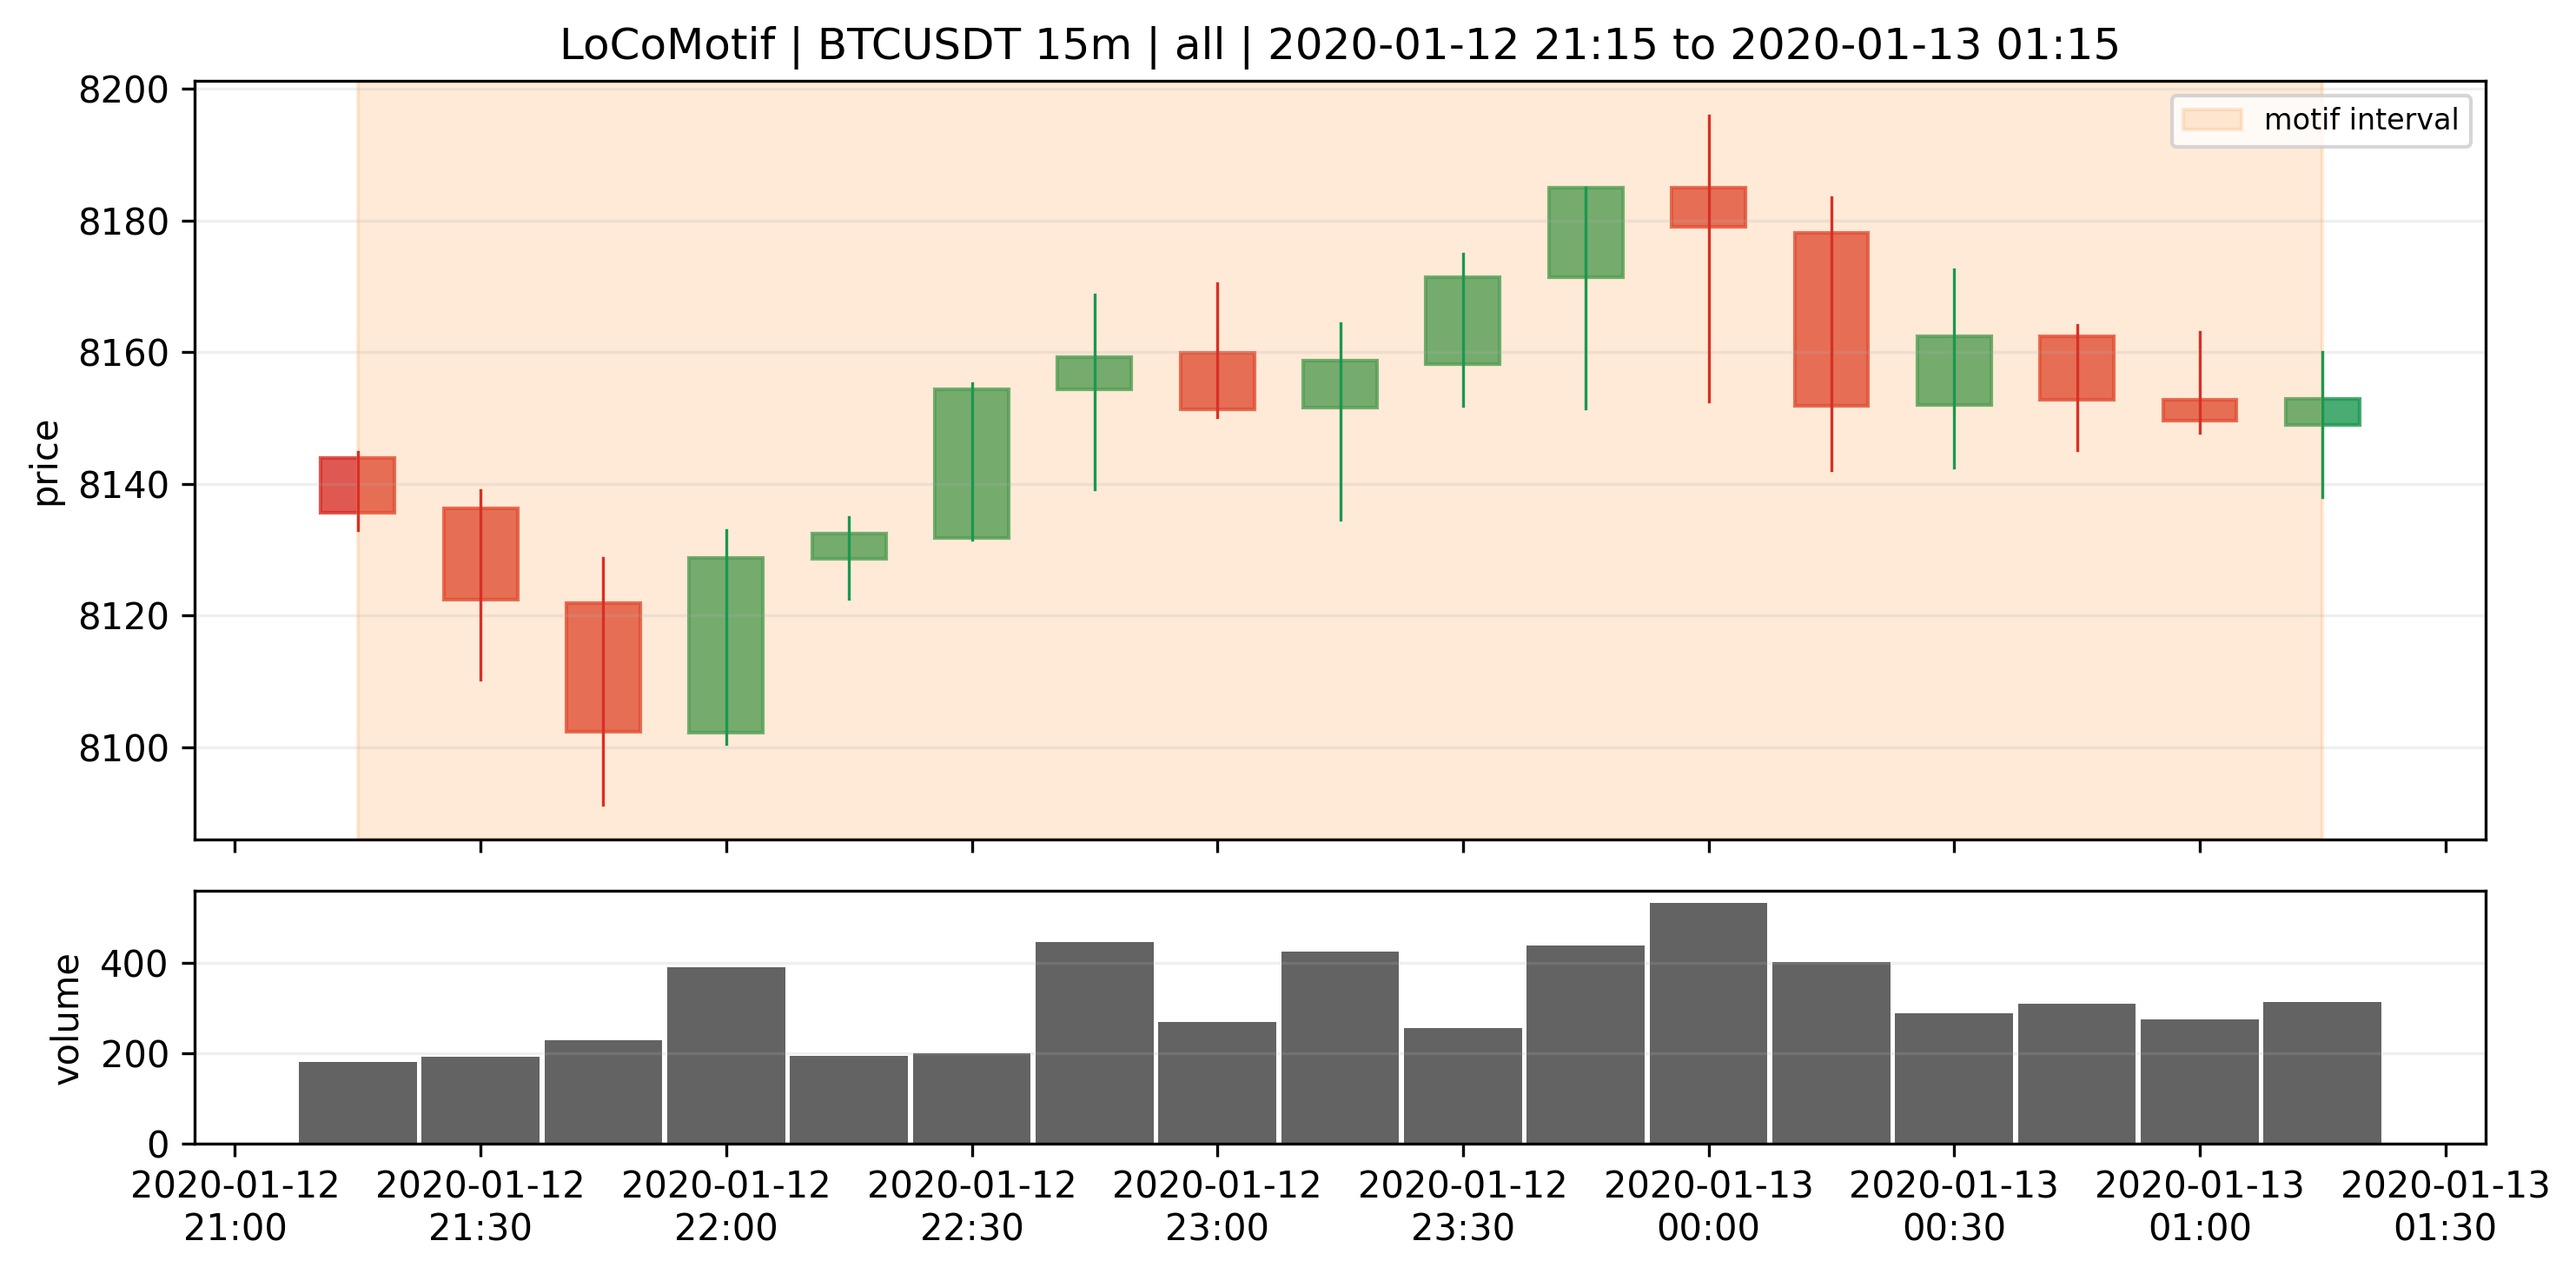
\includegraphics[width=0.9\linewidth]{reports/final_visual_evidence/figures/top_motif_08_locomotif_btcusdt_15m_all_zoom.png}
\caption{top motif 08 locomotif btcusdt 15m all zoom. The figure compares real available Matrix Profile and LoCoMotif outputs while preserving object-type differences.}
\end{figure}

\begin{figure}[ht]
\centering
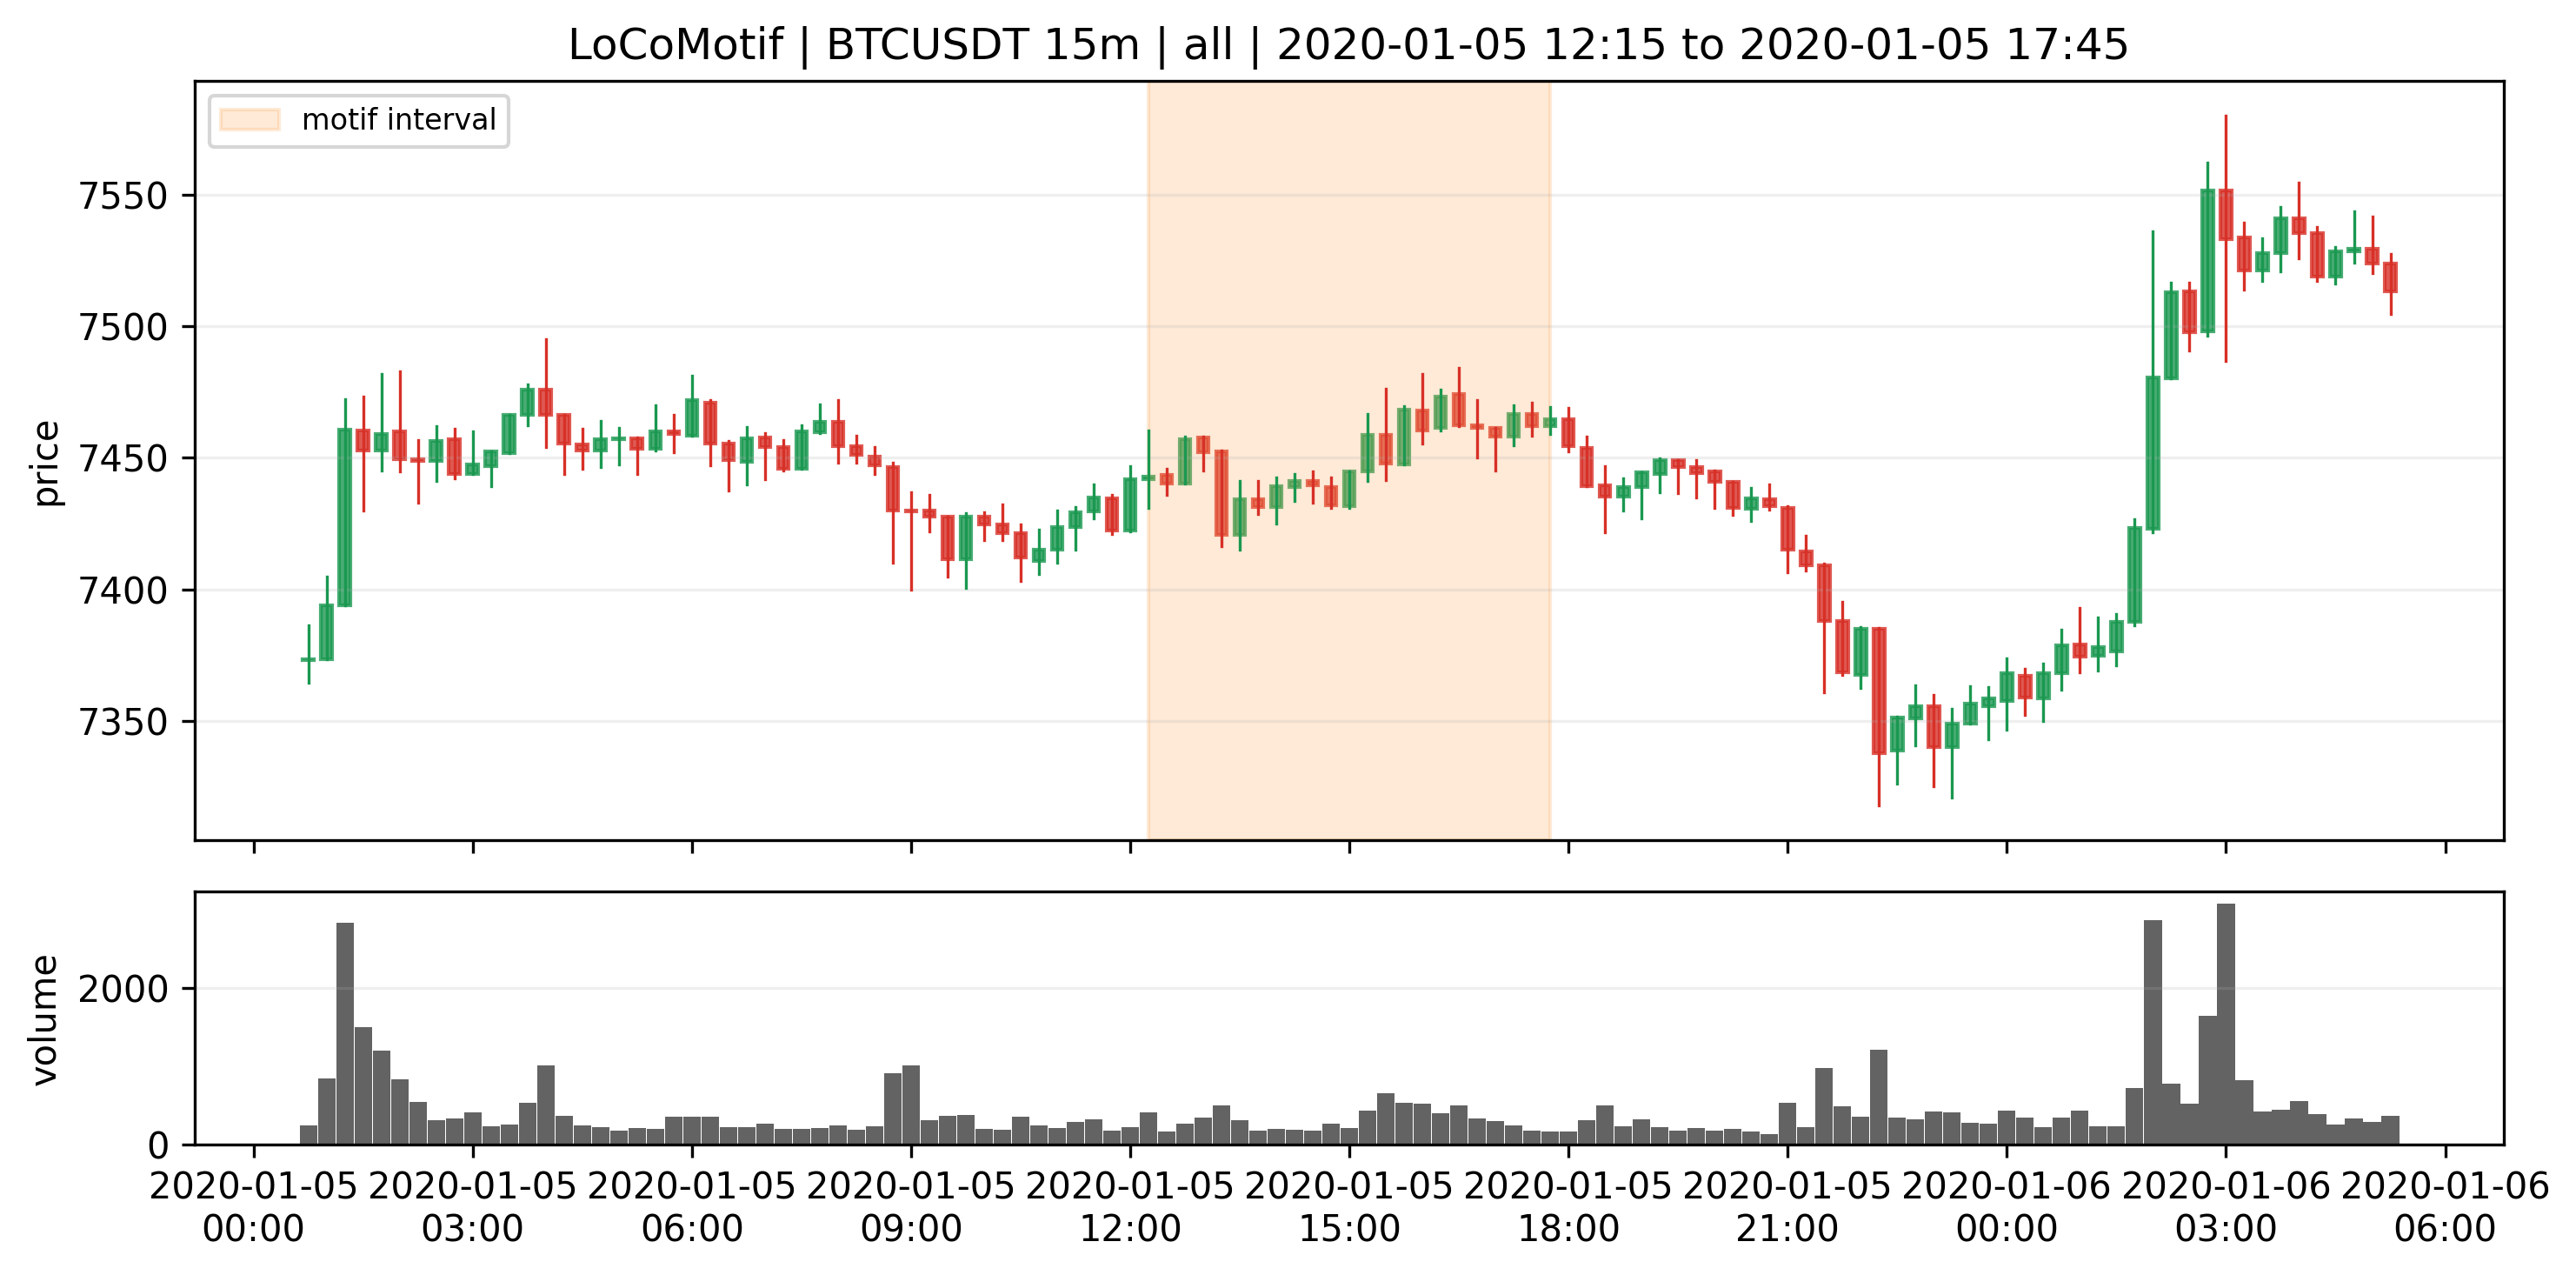
\includegraphics[width=0.9\linewidth]{reports/final_visual_evidence/figures/top_motif_09_locomotif_btcusdt_15m_all_context.png}
\caption{top motif 09 locomotif btcusdt 15m all context. The figure compares real available Matrix Profile and LoCoMotif outputs while preserving object-type differences.}
\end{figure}

\begin{figure}[ht]
\centering
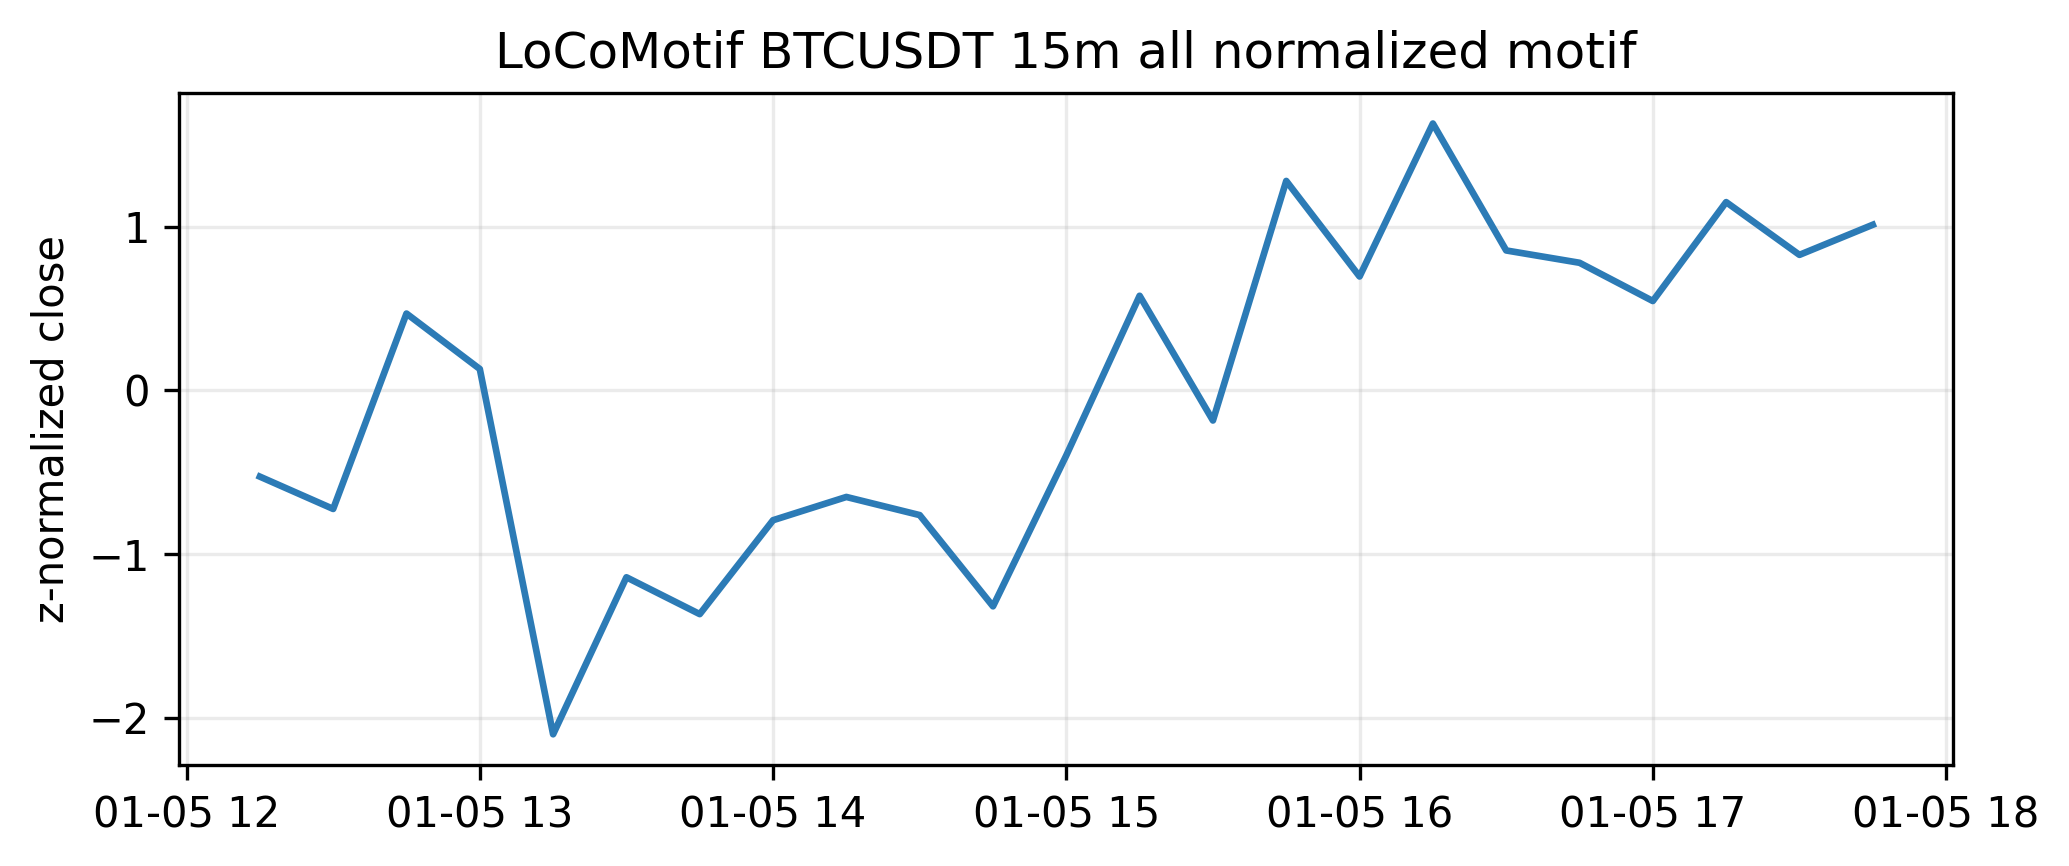
\includegraphics[width=0.9\linewidth]{reports/final_visual_evidence/figures/top_motif_09_locomotif_btcusdt_15m_all_normal_pattern.png}
\caption{top motif 09 locomotif btcusdt 15m all normal pattern. The figure compares real available Matrix Profile and LoCoMotif outputs while preserving object-type differences.}
\end{figure}

\begin{figure}[ht]
\centering
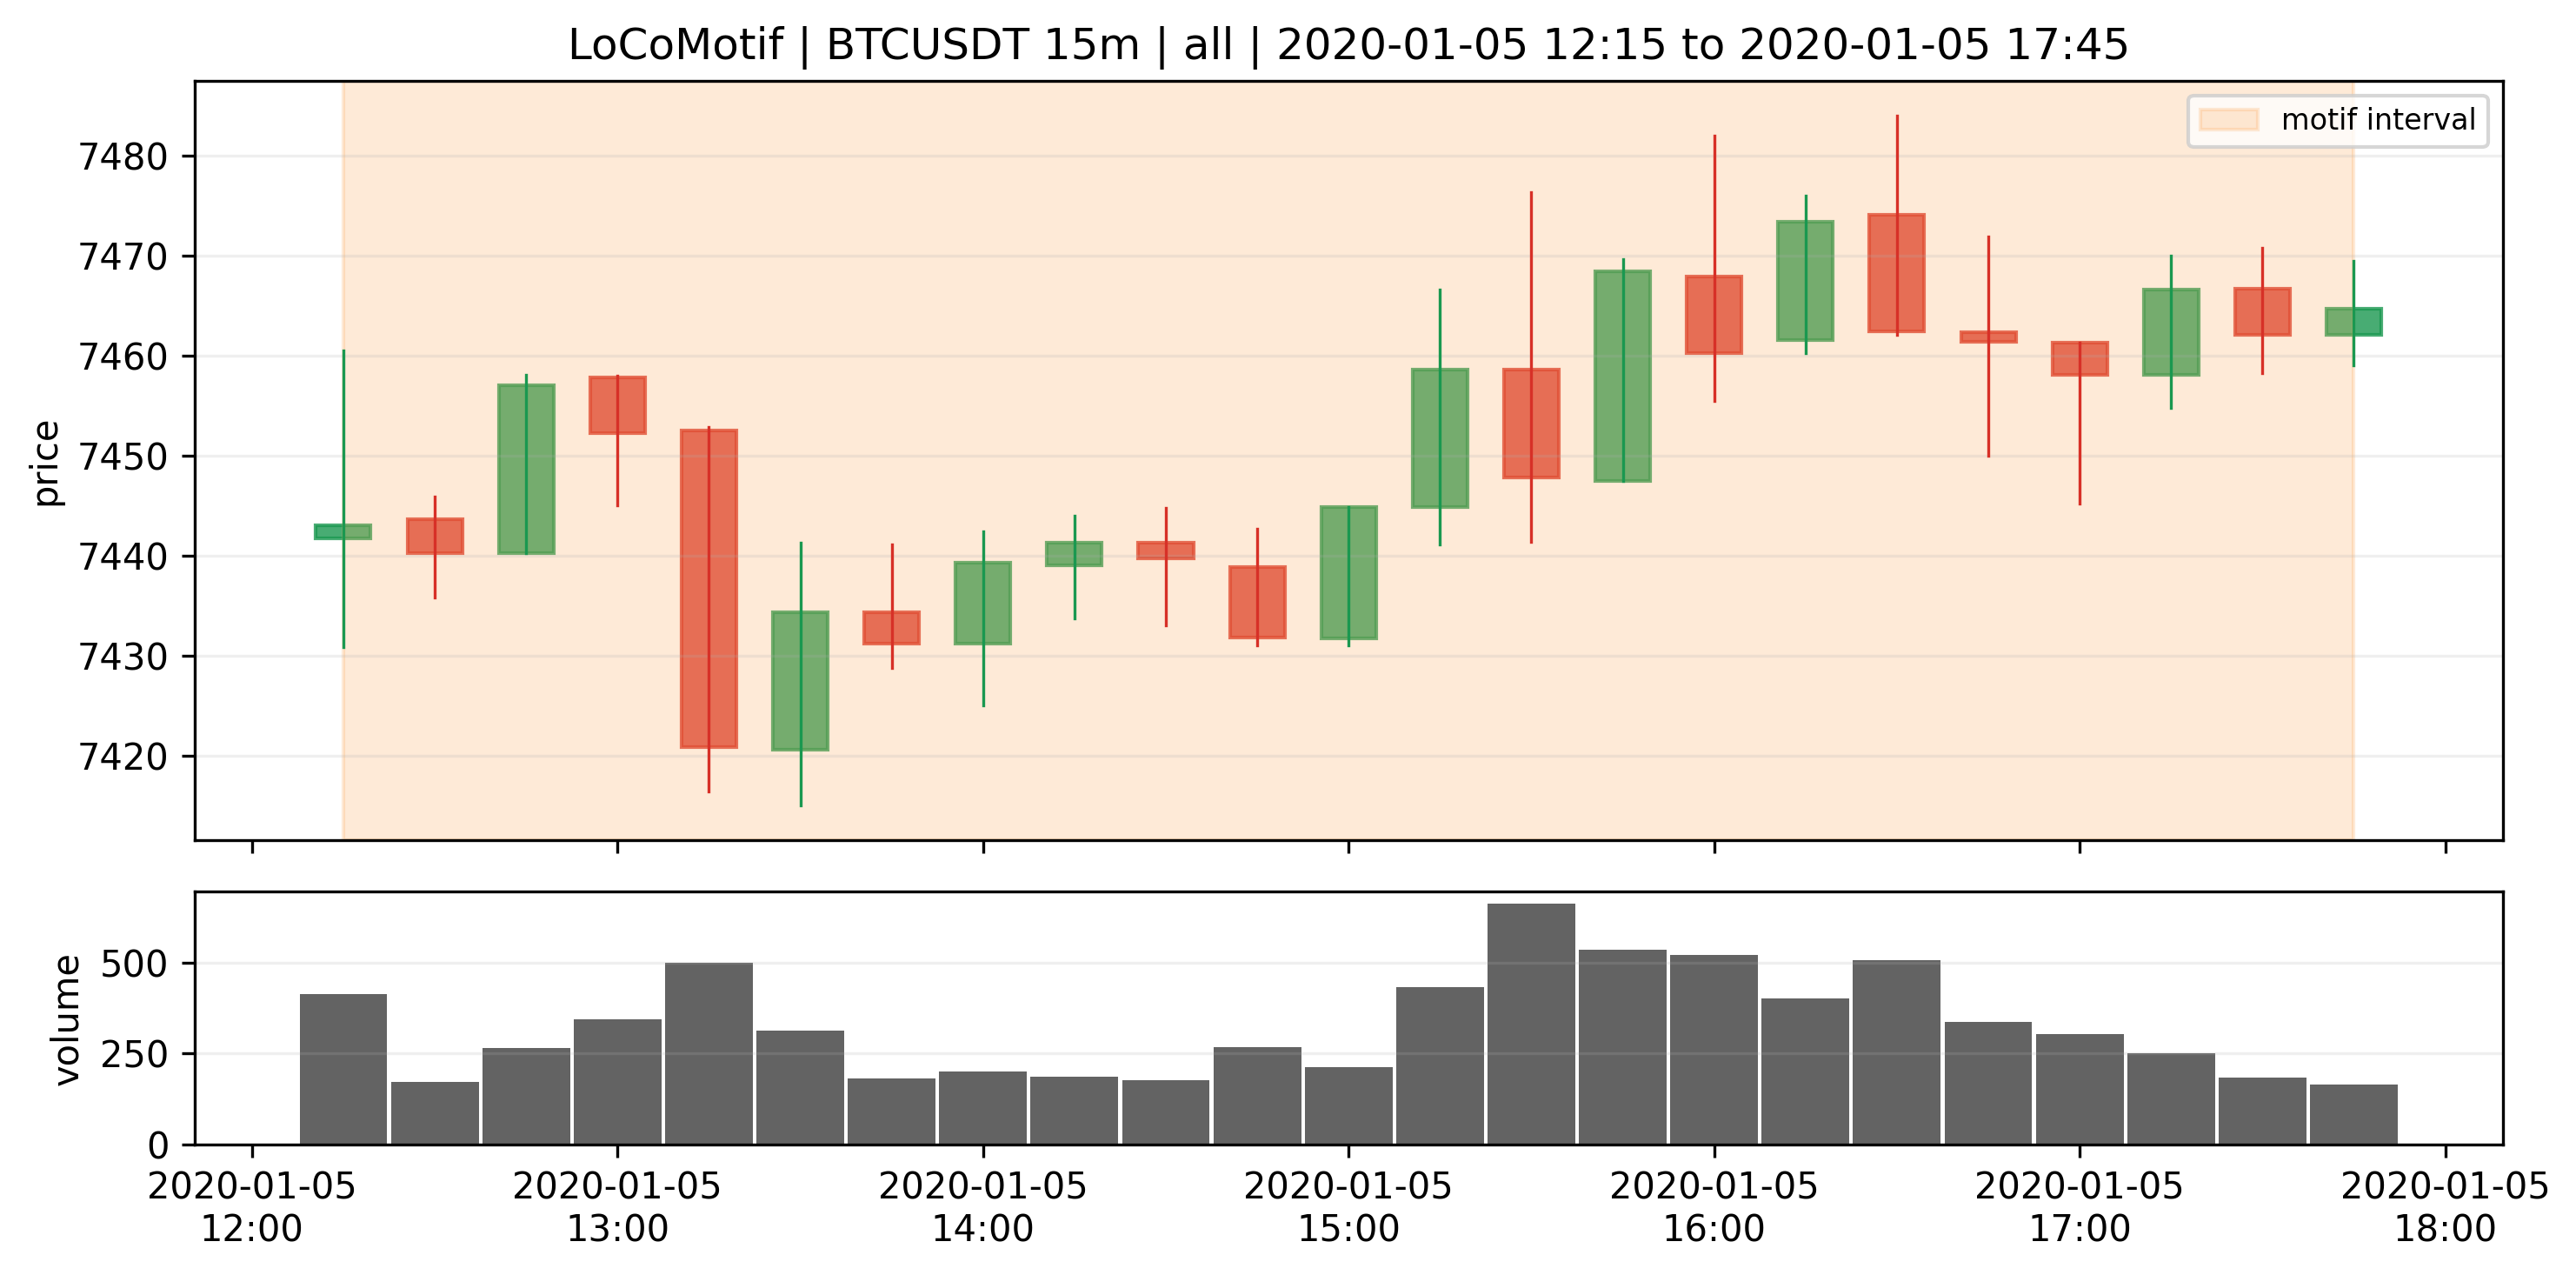
\includegraphics[width=0.9\linewidth]{reports/final_visual_evidence/figures/top_motif_09_locomotif_btcusdt_15m_all_zoom.png}
\caption{top motif 09 locomotif btcusdt 15m all zoom. The figure compares real available Matrix Profile and LoCoMotif outputs while preserving object-type differences.}
\end{figure}

\begin{figure}[ht]
\centering
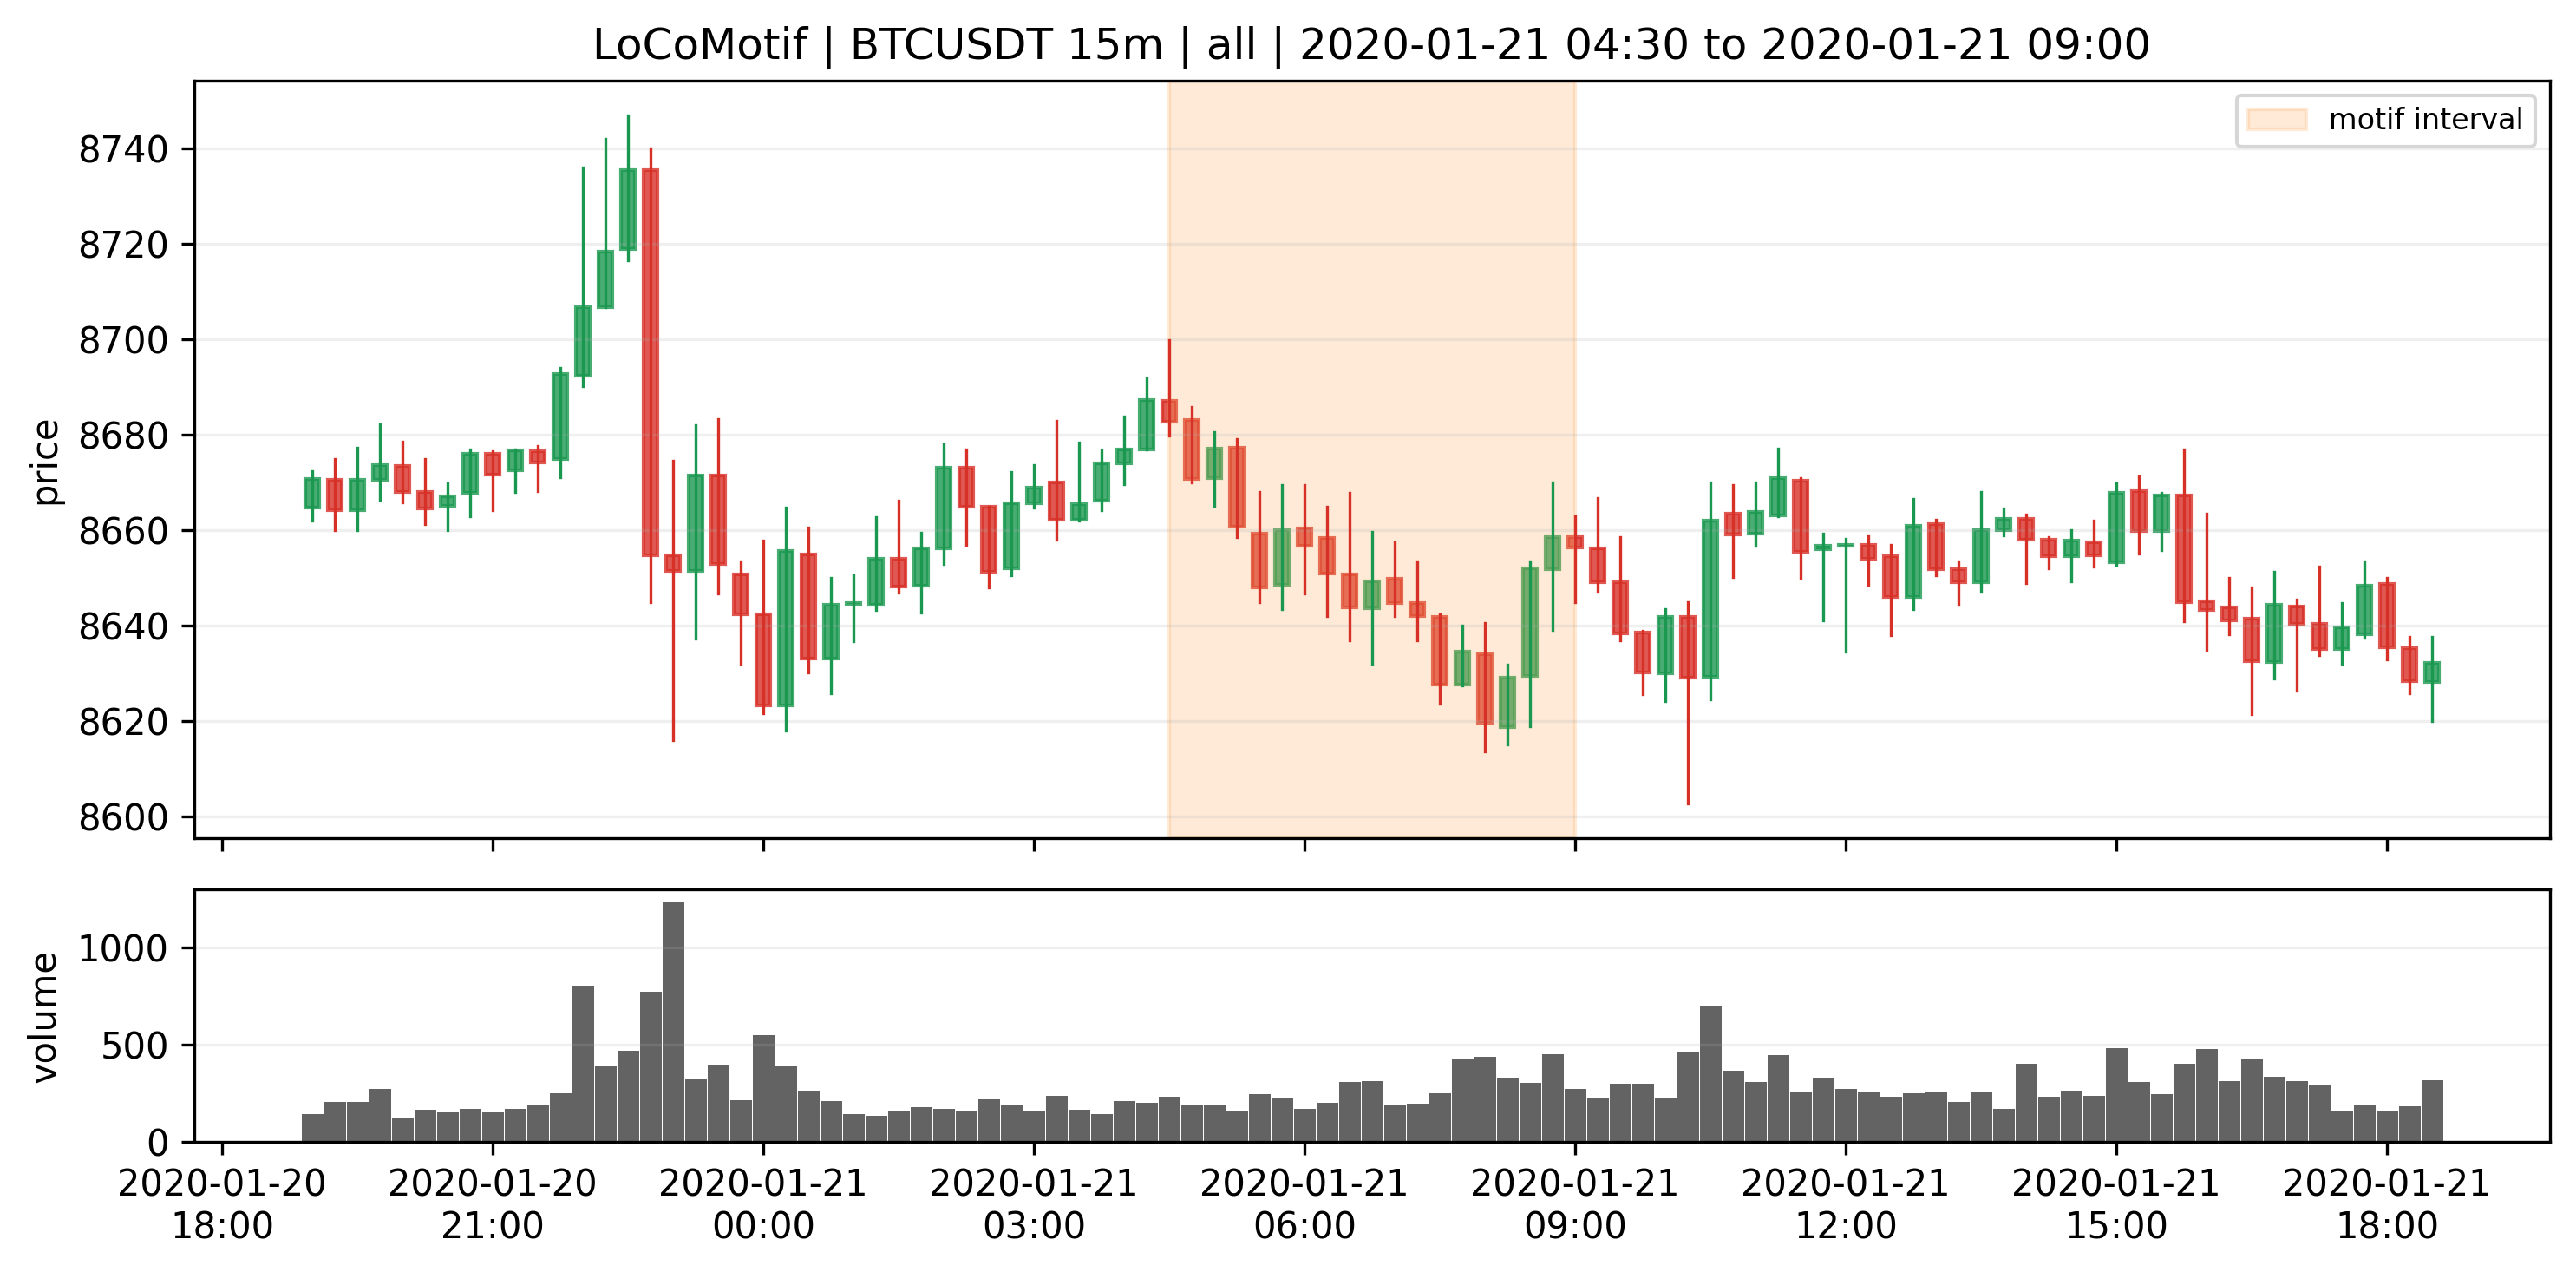
\includegraphics[width=0.9\linewidth]{reports/final_visual_evidence/figures/top_motif_10_locomotif_btcusdt_15m_all_context.png}
\caption{top motif 10 locomotif btcusdt 15m all context. The figure compares real available Matrix Profile and LoCoMotif outputs while preserving object-type differences.}
\end{figure}

\begin{figure}[ht]
\centering
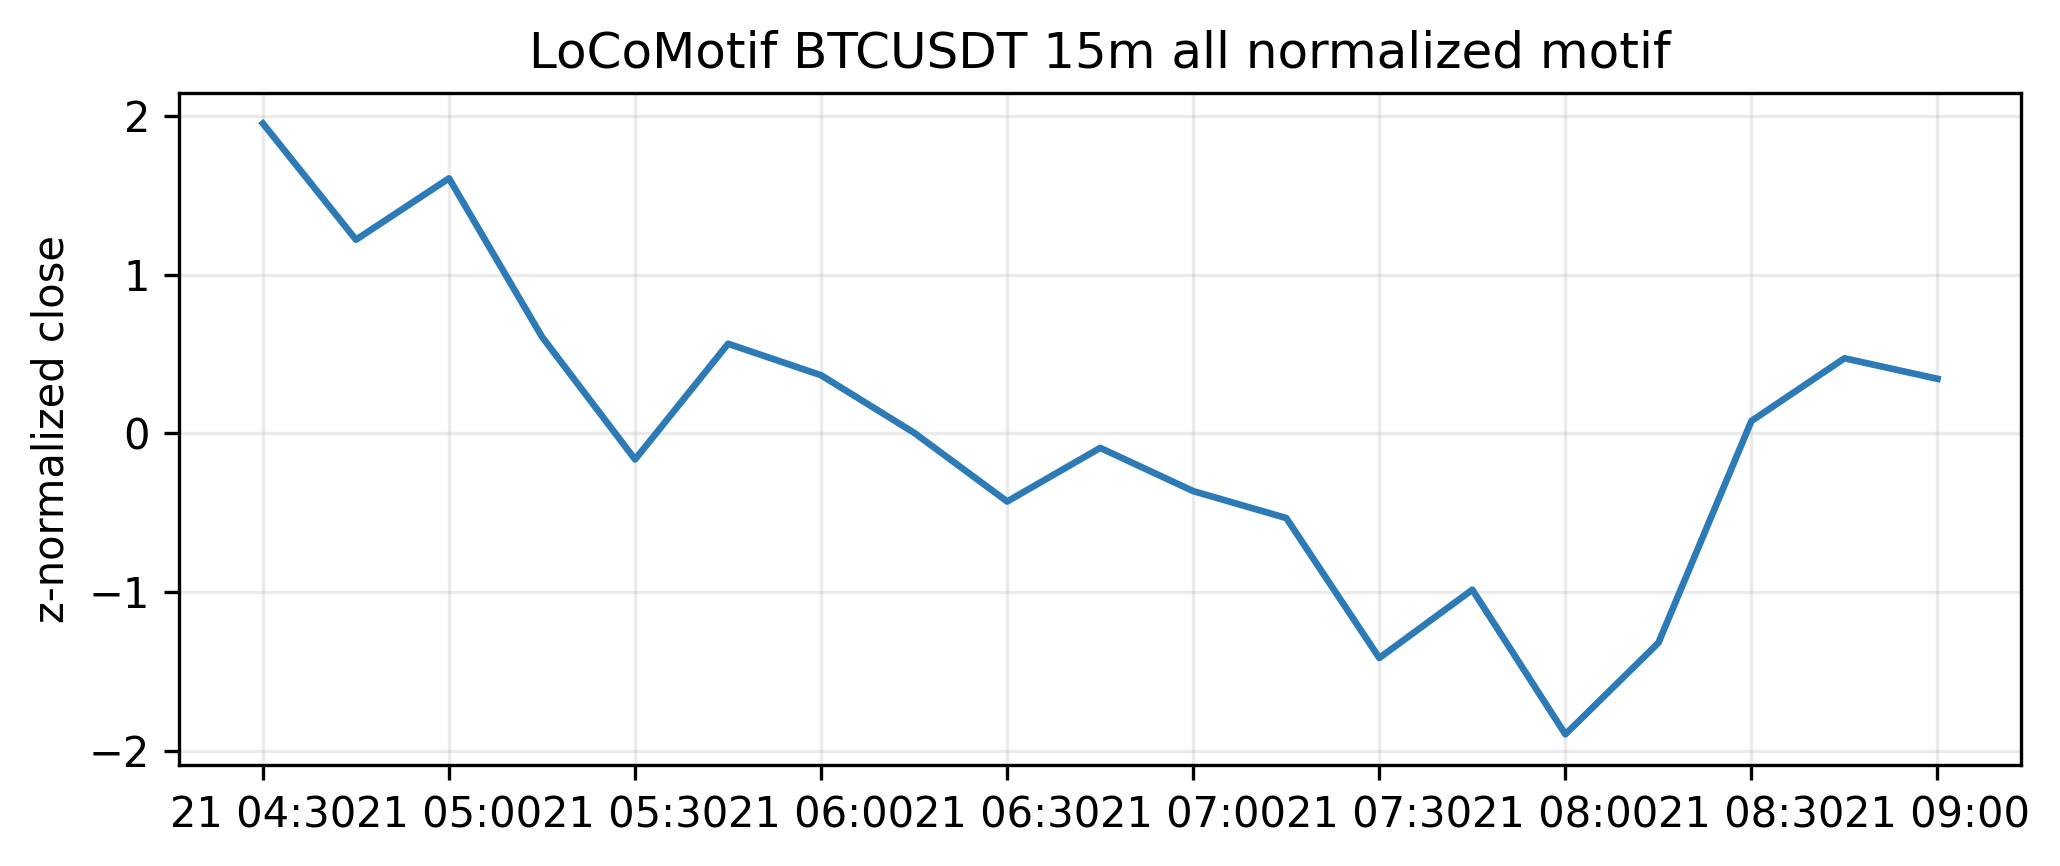
\includegraphics[width=0.9\linewidth]{reports/final_visual_evidence/figures/top_motif_10_locomotif_btcusdt_15m_all_normal_pattern.png}
\caption{top motif 10 locomotif btcusdt 15m all normal pattern. The figure compares real available Matrix Profile and LoCoMotif outputs while preserving object-type differences.}
\end{figure}

\begin{figure}[ht]
\centering
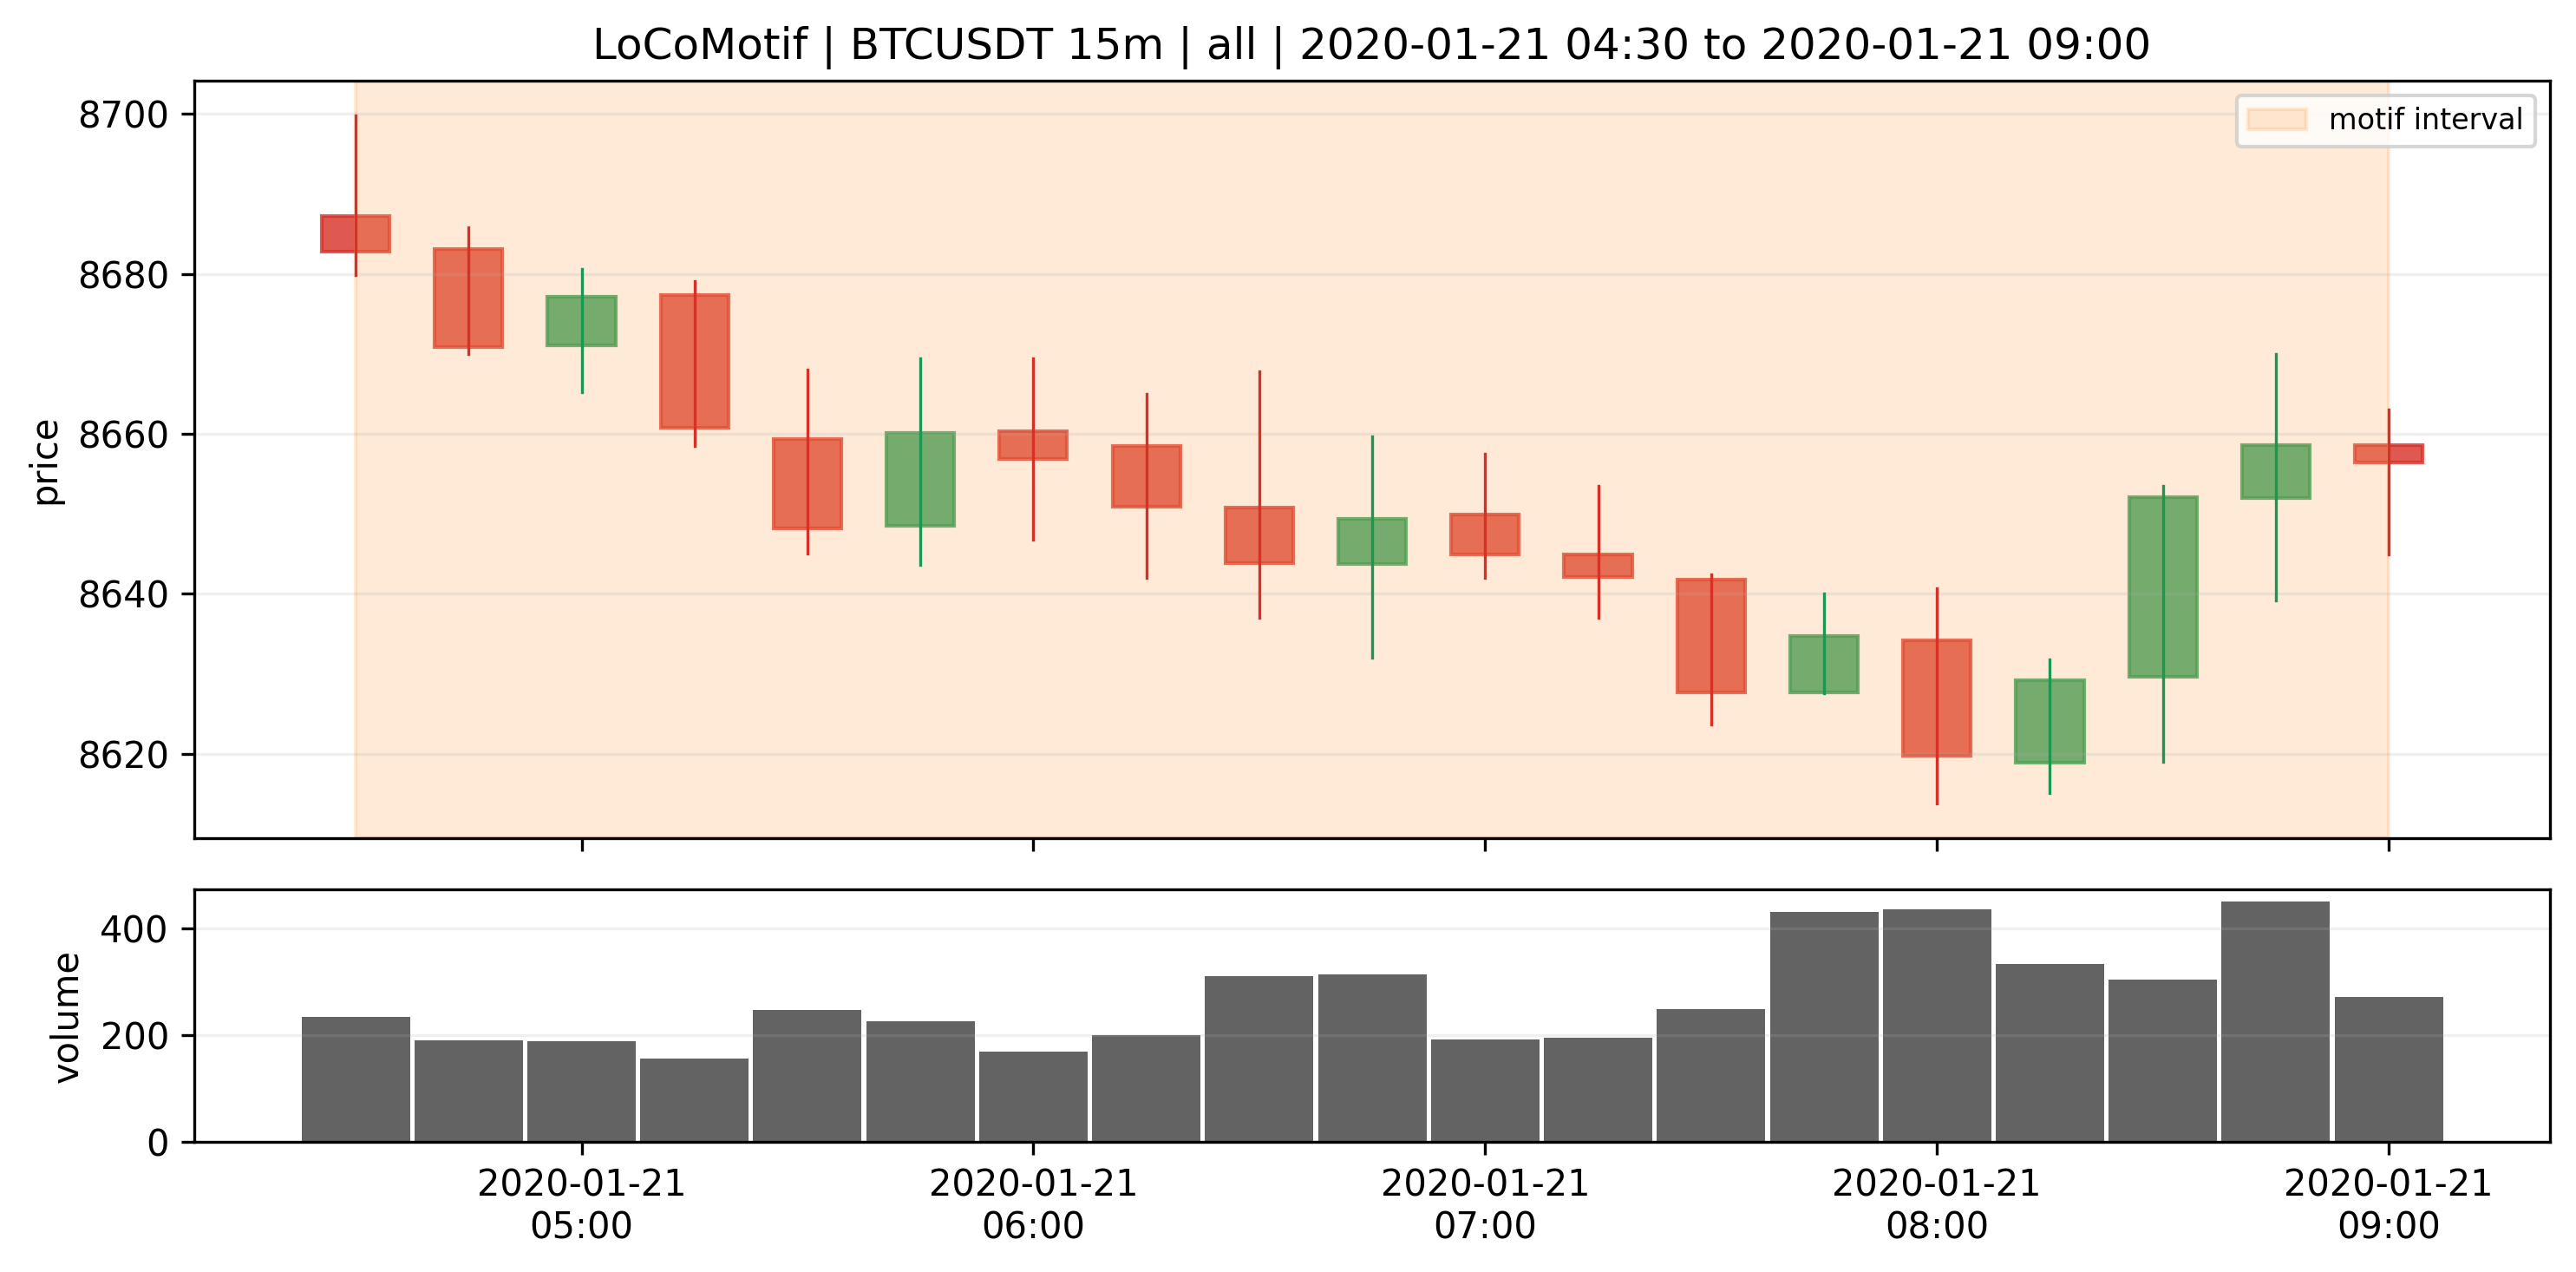
\includegraphics[width=0.9\linewidth]{reports/final_visual_evidence/figures/top_motif_10_locomotif_btcusdt_15m_all_zoom.png}
\caption{top motif 10 locomotif btcusdt 15m all zoom. The figure compares real available Matrix Profile and LoCoMotif outputs while preserving object-type differences.}
\end{figure}

\begin{figure}[ht]
\centering
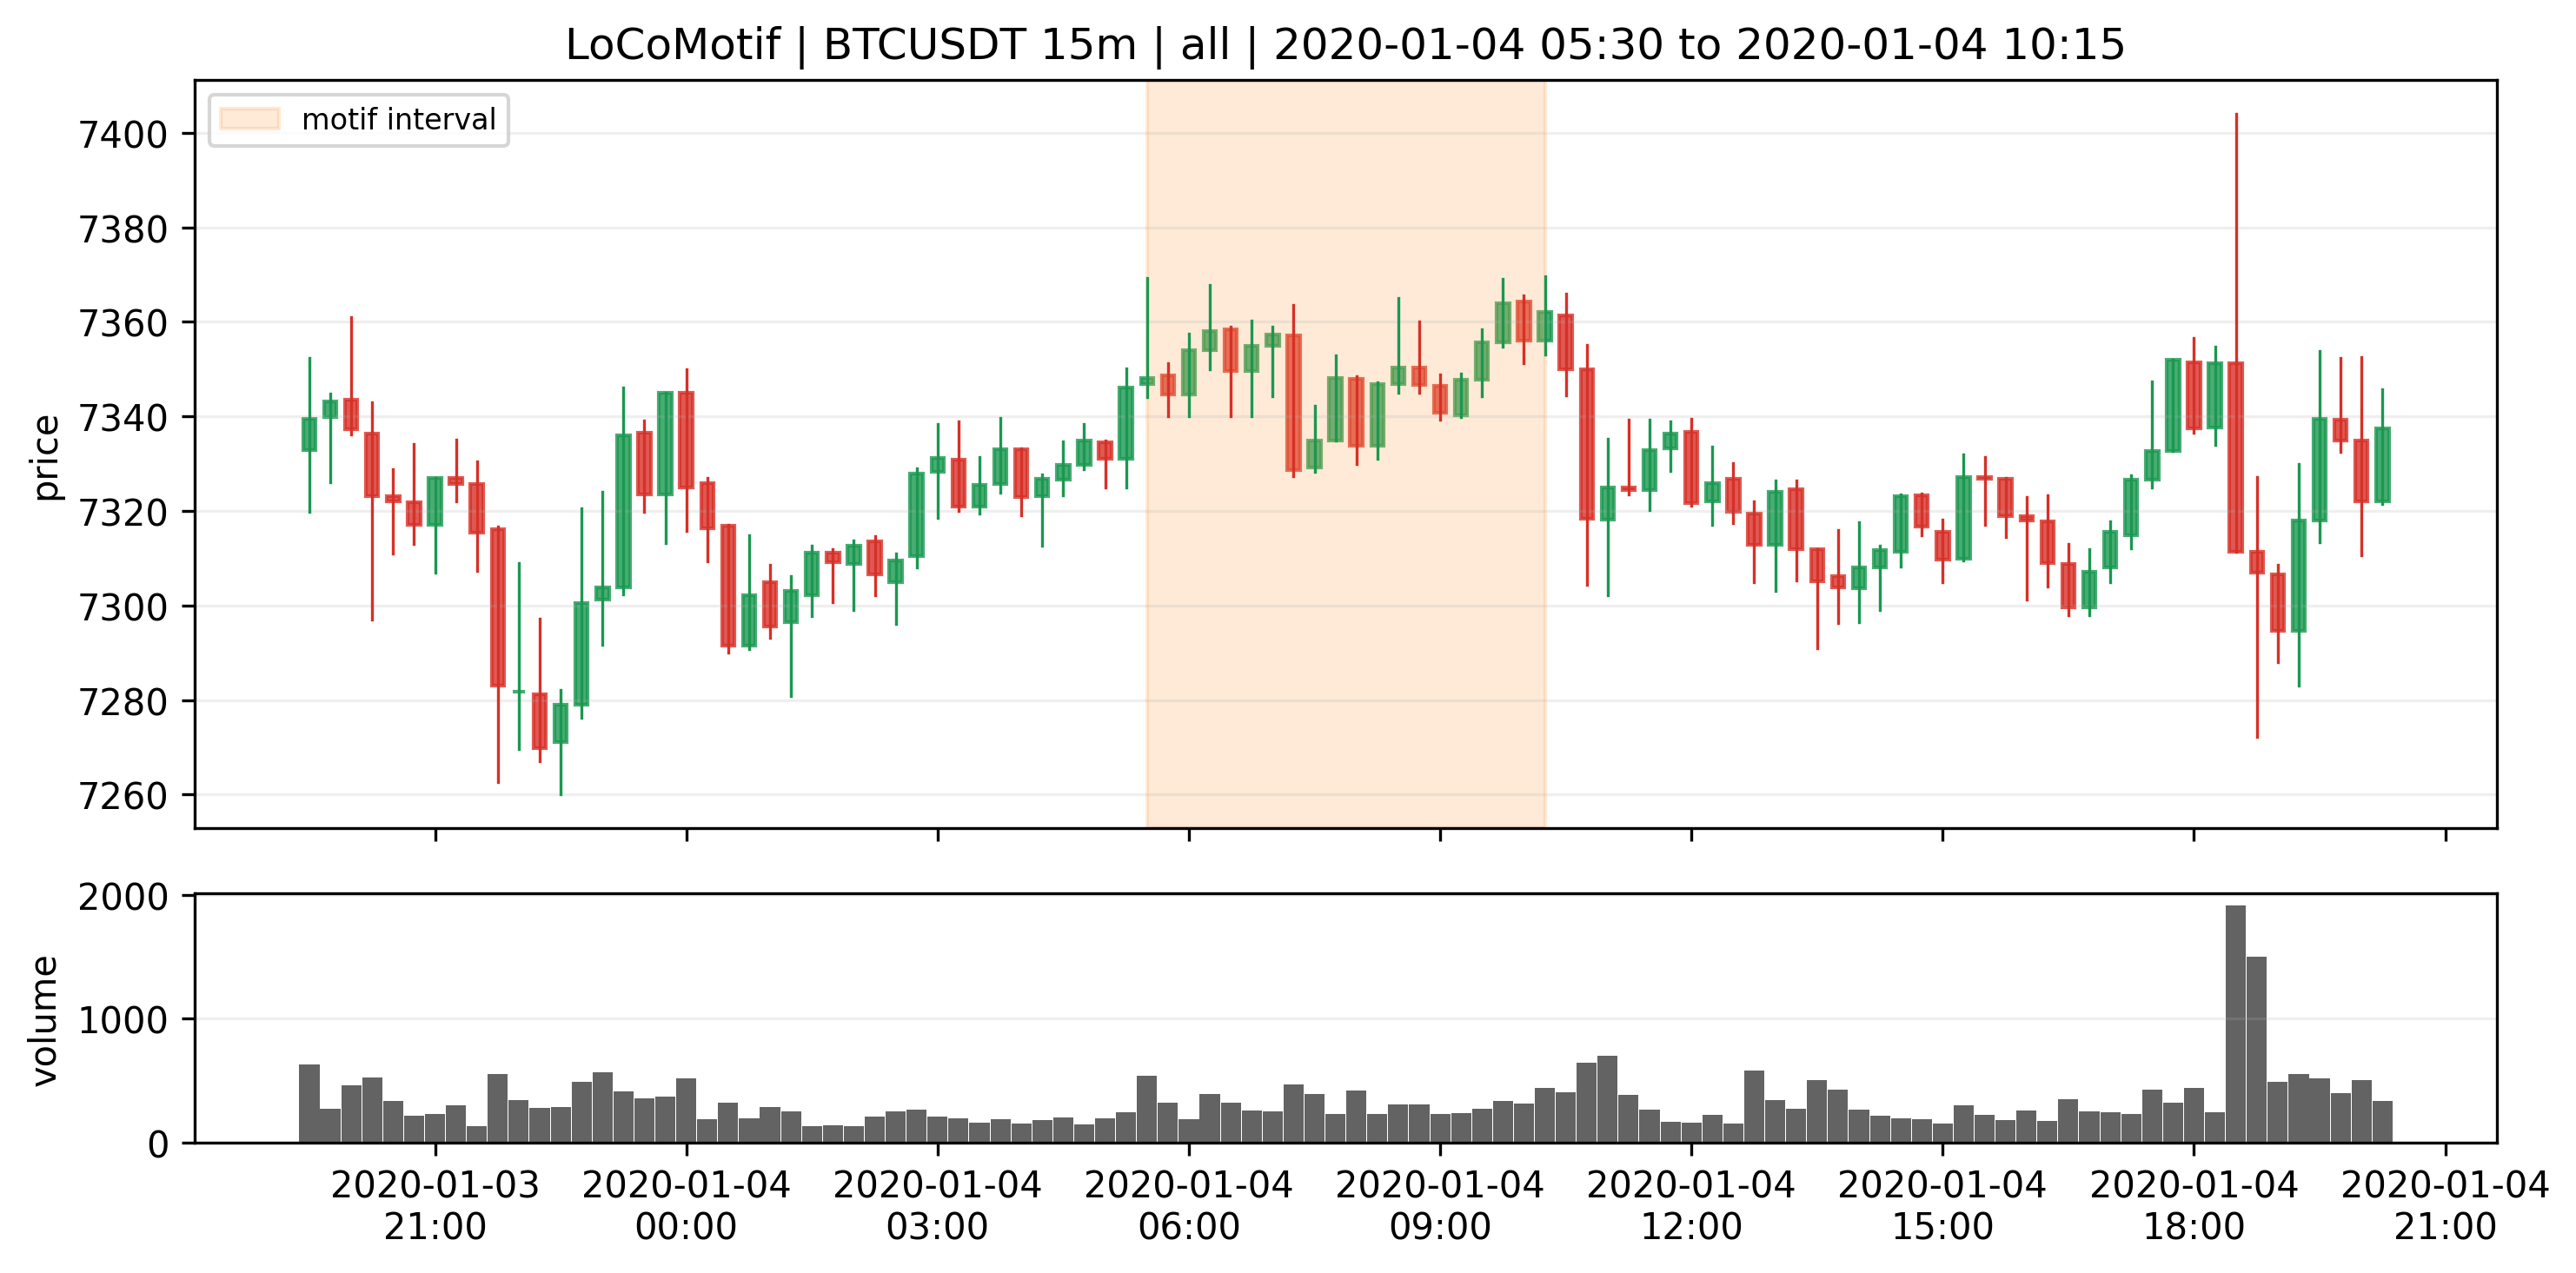
\includegraphics[width=0.9\linewidth]{reports/final_visual_evidence/figures/top_motif_11_locomotif_btcusdt_15m_all_context.png}
\caption{top motif 11 locomotif btcusdt 15m all context. The figure compares real available Matrix Profile and LoCoMotif outputs while preserving object-type differences.}
\end{figure}

\begin{figure}[ht]
\centering
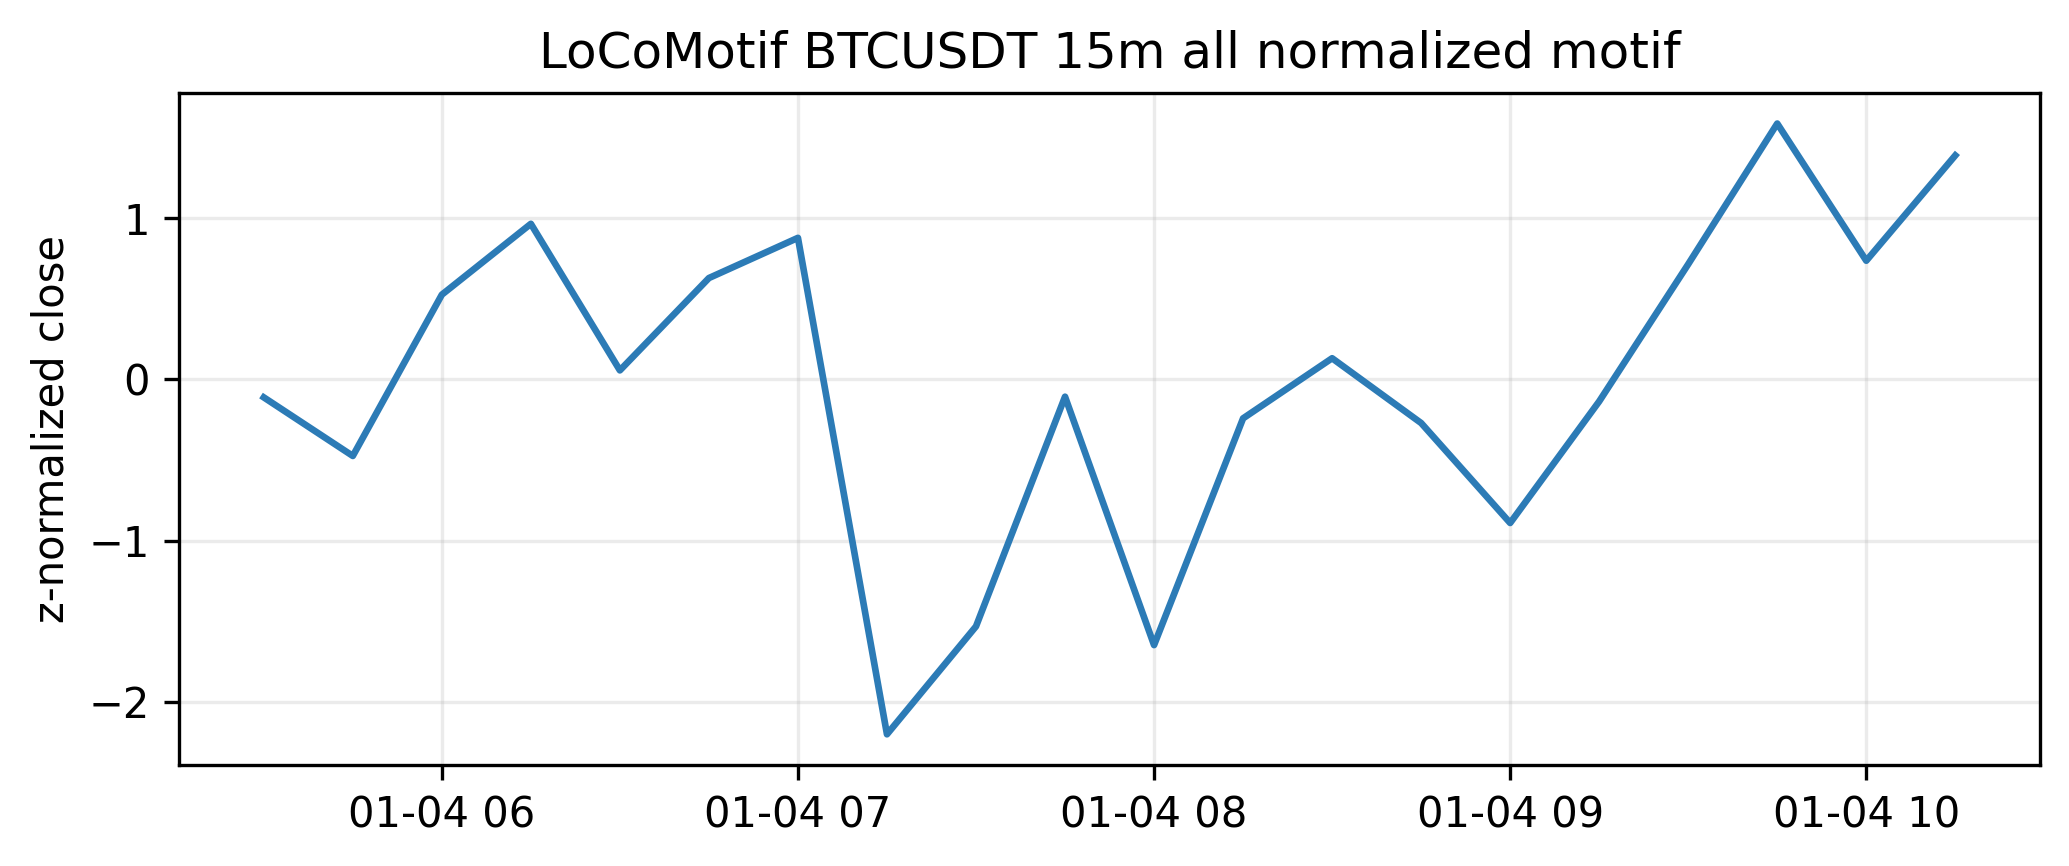
\includegraphics[width=0.9\linewidth]{reports/final_visual_evidence/figures/top_motif_11_locomotif_btcusdt_15m_all_normal_pattern.png}
\caption{top motif 11 locomotif btcusdt 15m all normal pattern. The figure compares real available Matrix Profile and LoCoMotif outputs while preserving object-type differences.}
\end{figure}

\begin{figure}[ht]
\centering
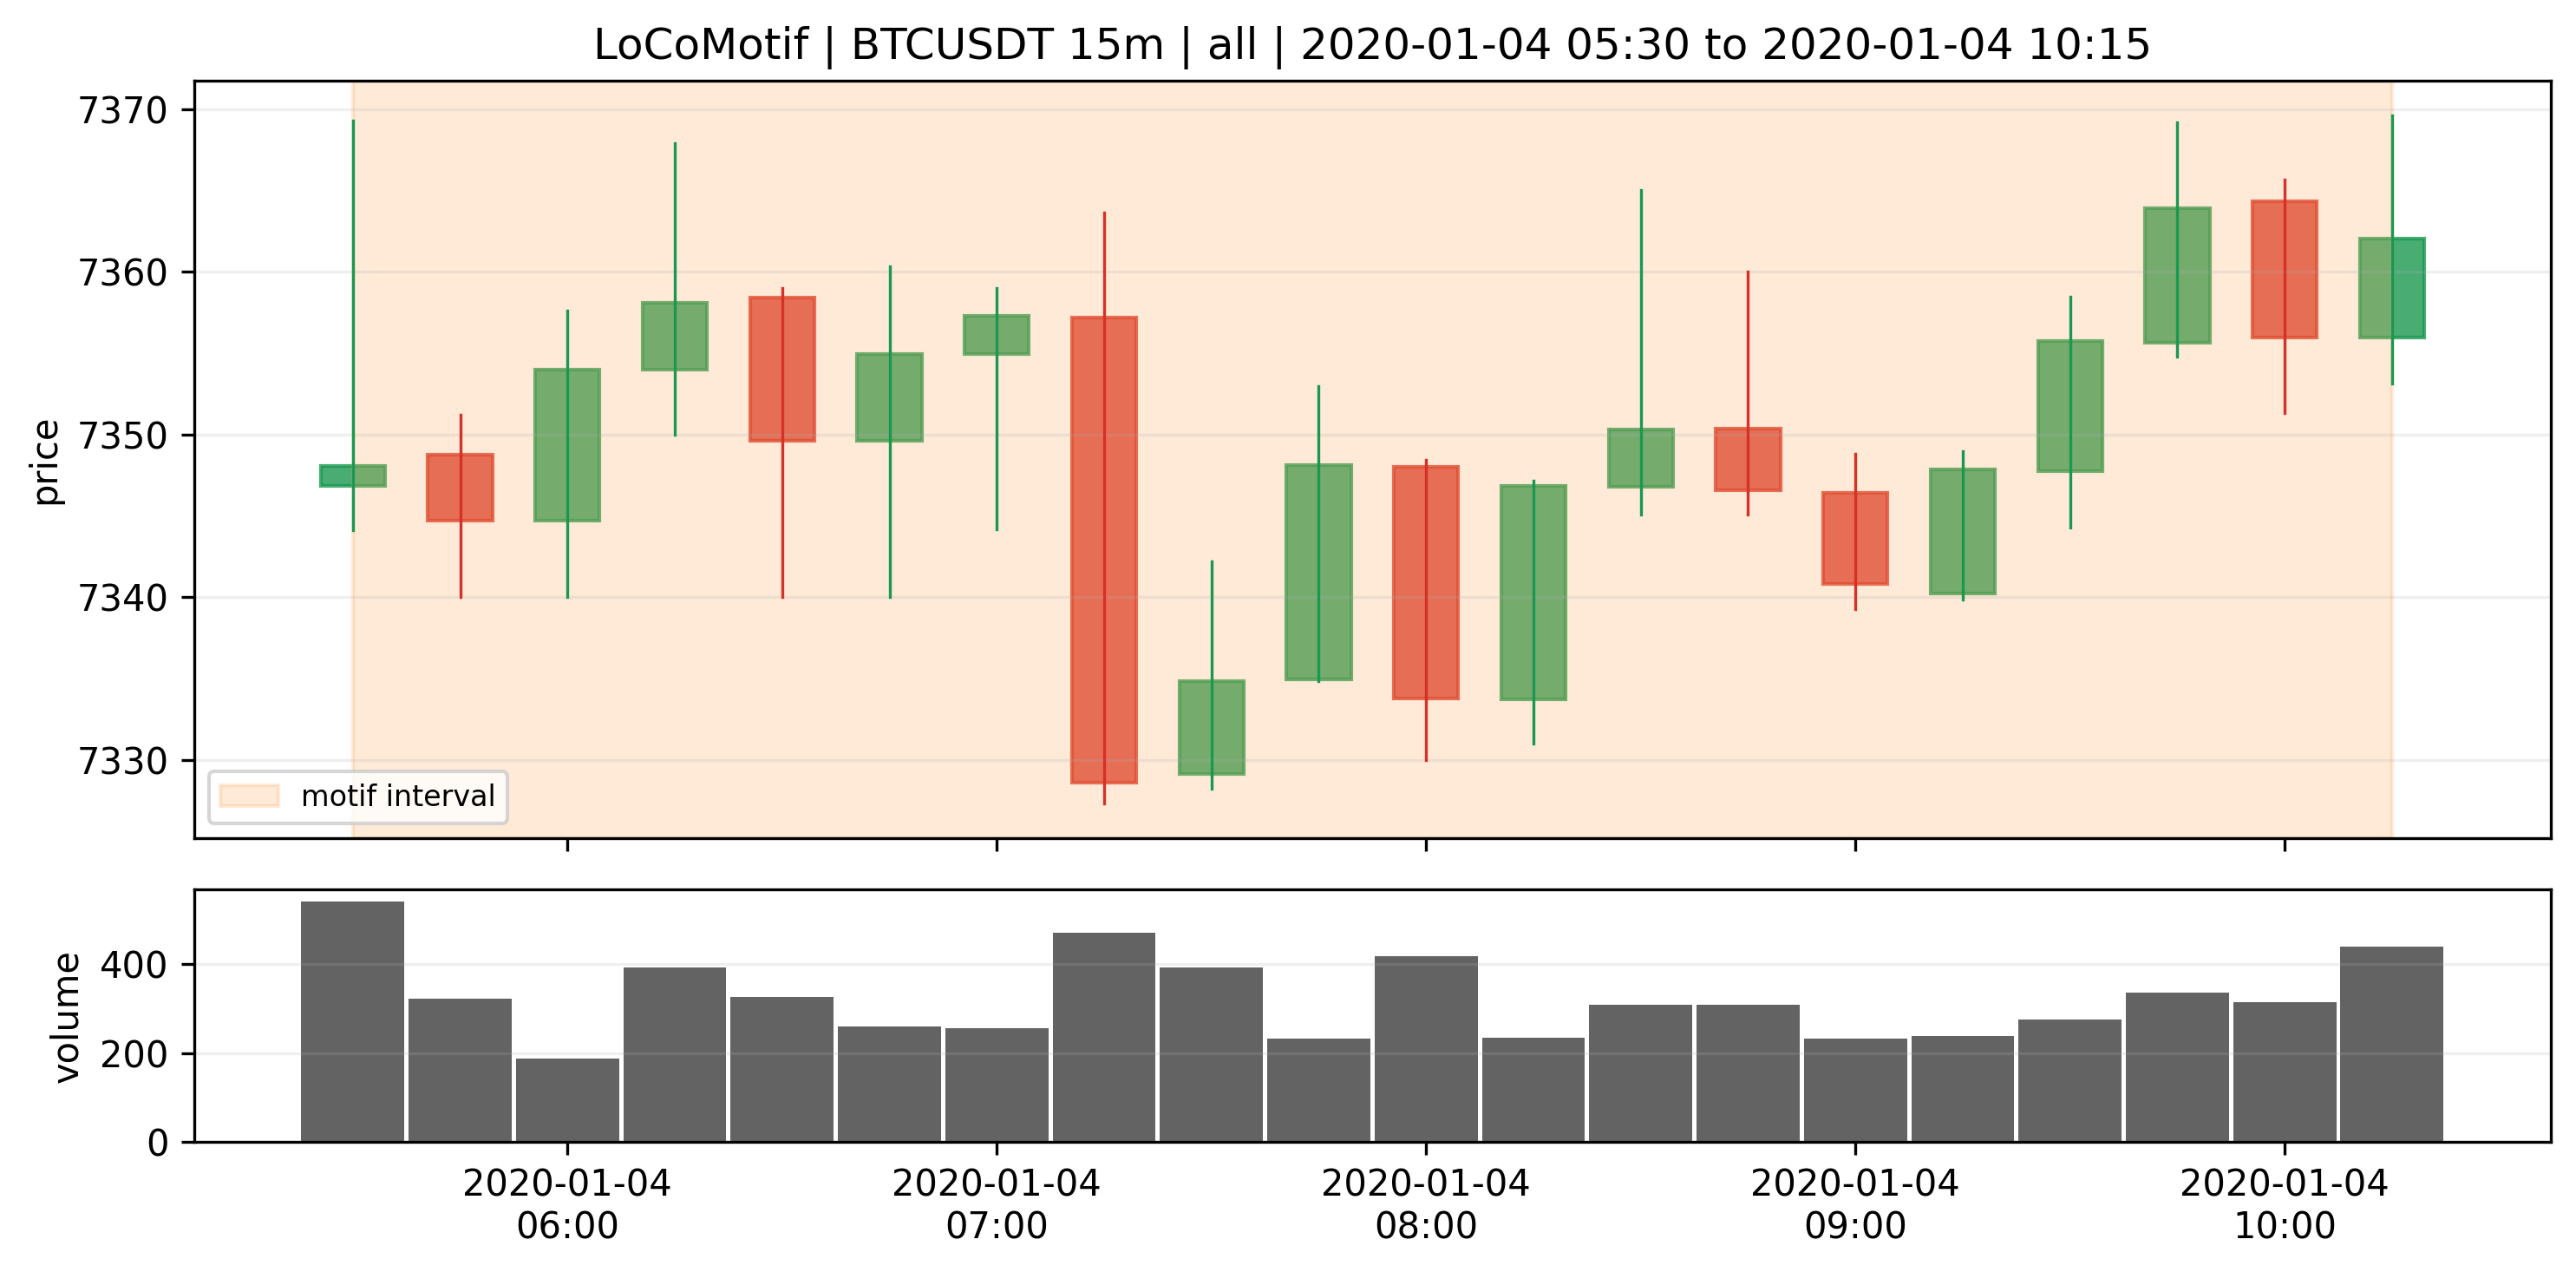
\includegraphics[width=0.9\linewidth]{reports/final_visual_evidence/figures/top_motif_11_locomotif_btcusdt_15m_all_zoom.png}
\caption{top motif 11 locomotif btcusdt 15m all zoom. The figure compares real available Matrix Profile and LoCoMotif outputs while preserving object-type differences.}
\end{figure}

\begin{figure}[ht]
\centering
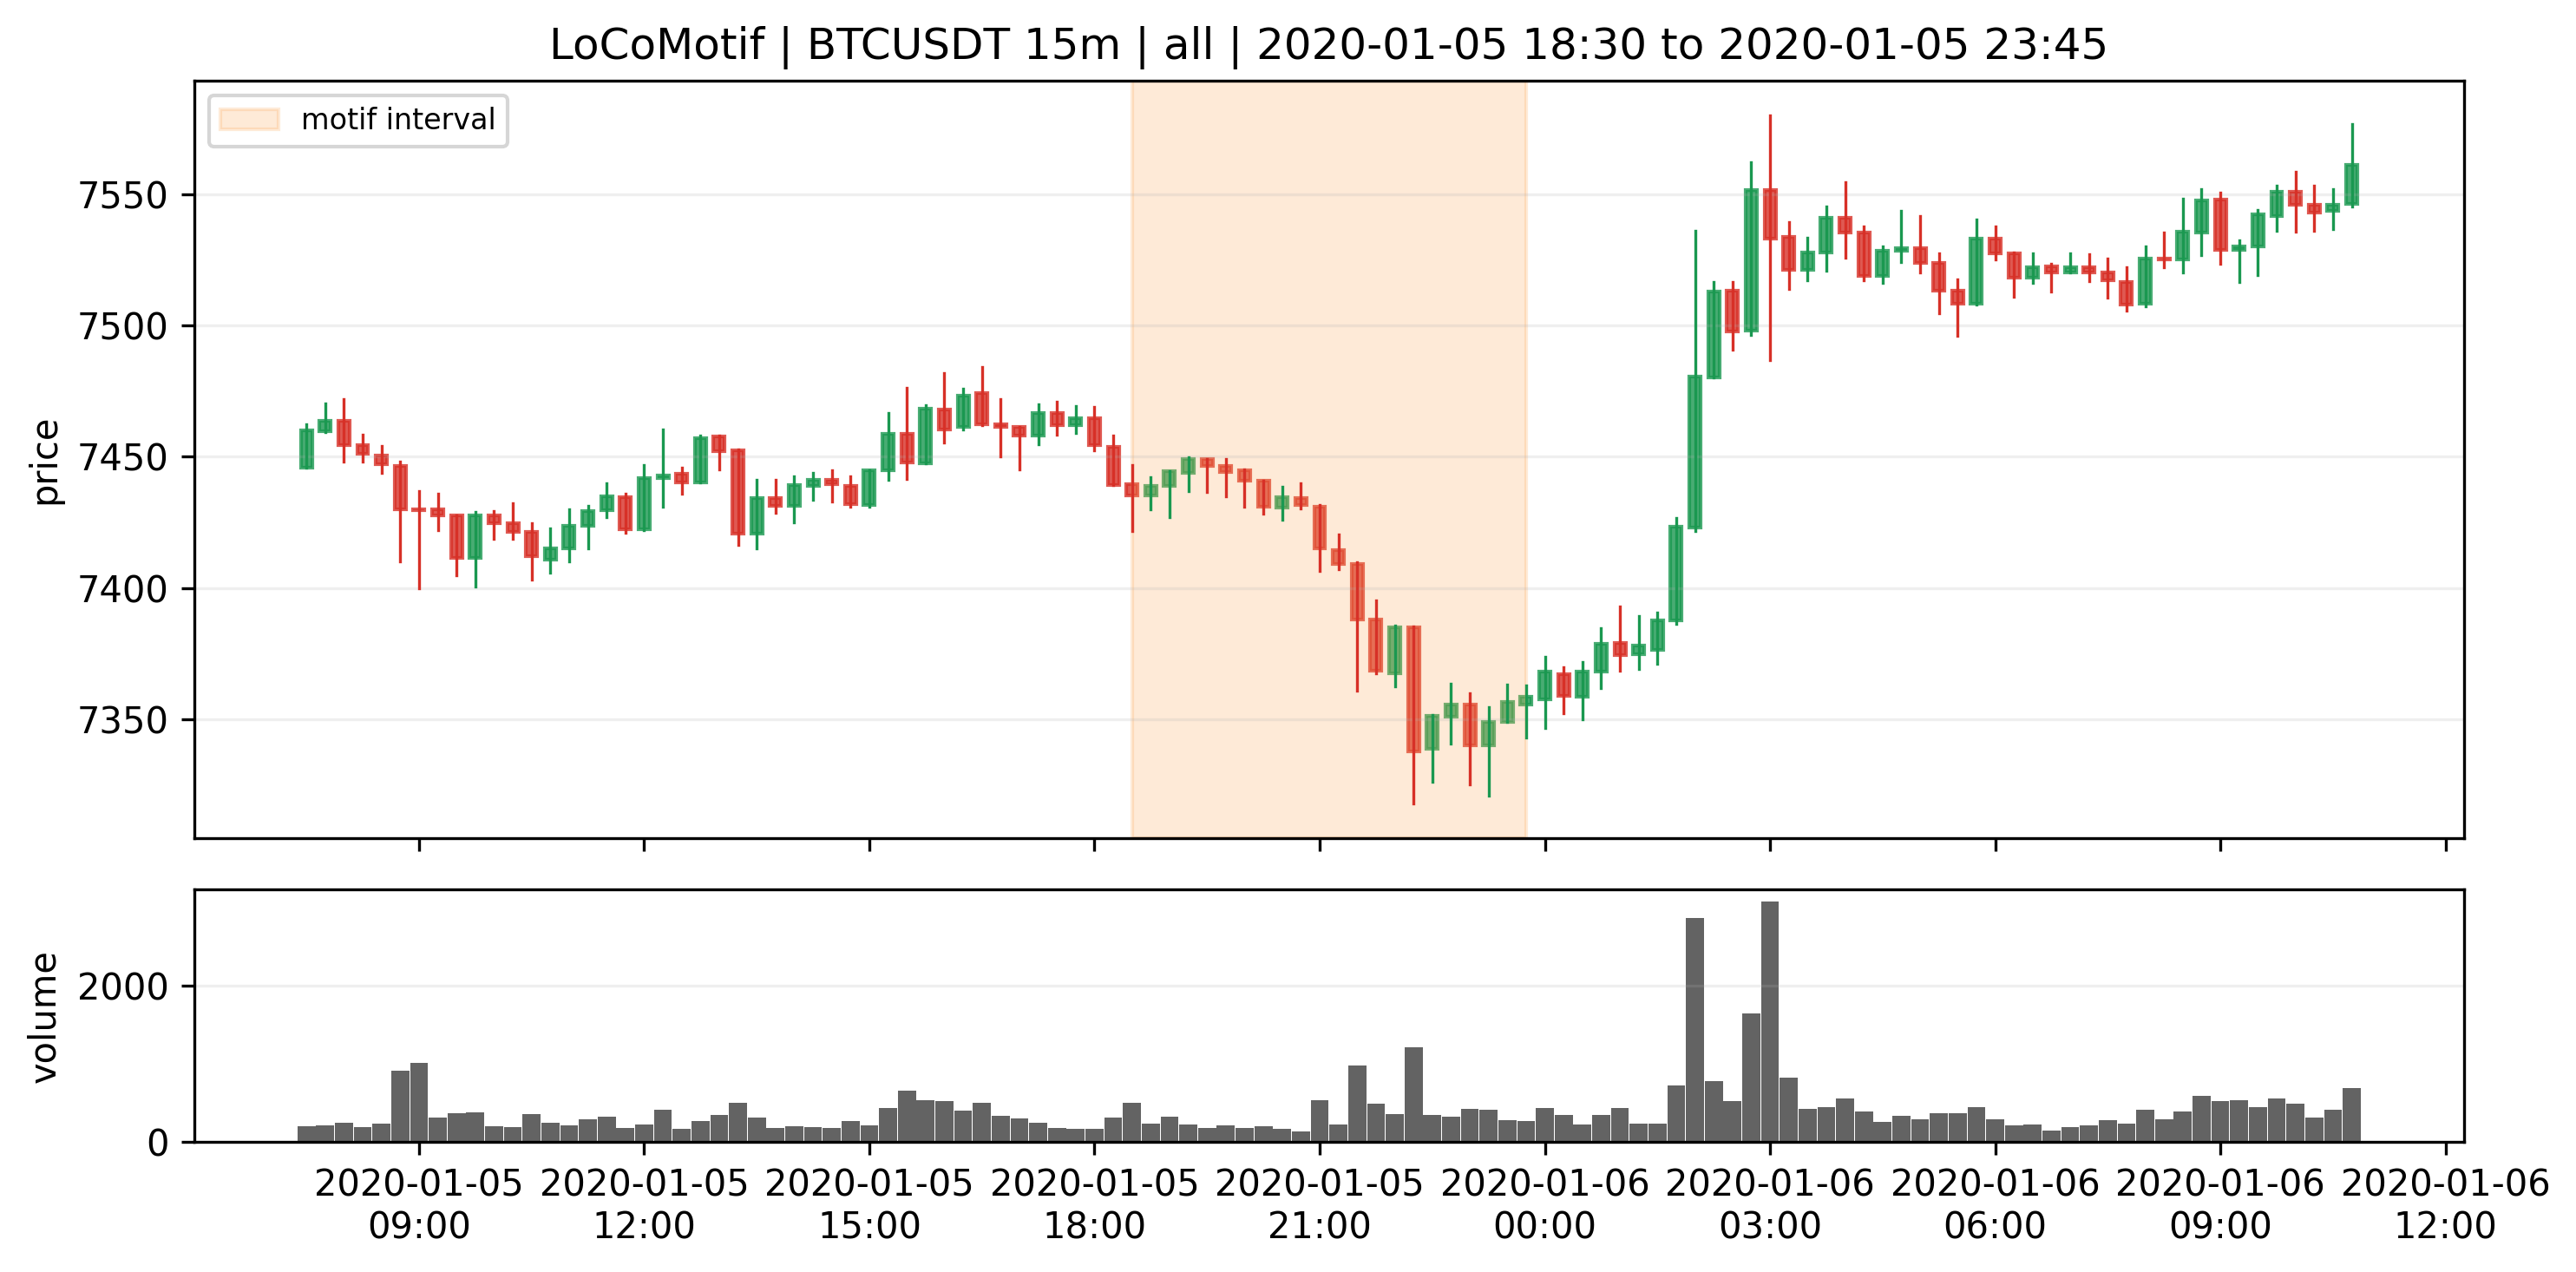
\includegraphics[width=0.9\linewidth]{reports/final_visual_evidence/figures/top_motif_12_locomotif_btcusdt_15m_all_context.png}
\caption{top motif 12 locomotif btcusdt 15m all context. The figure compares real available Matrix Profile and LoCoMotif outputs while preserving object-type differences.}
\end{figure}

\begin{figure}[ht]
\centering
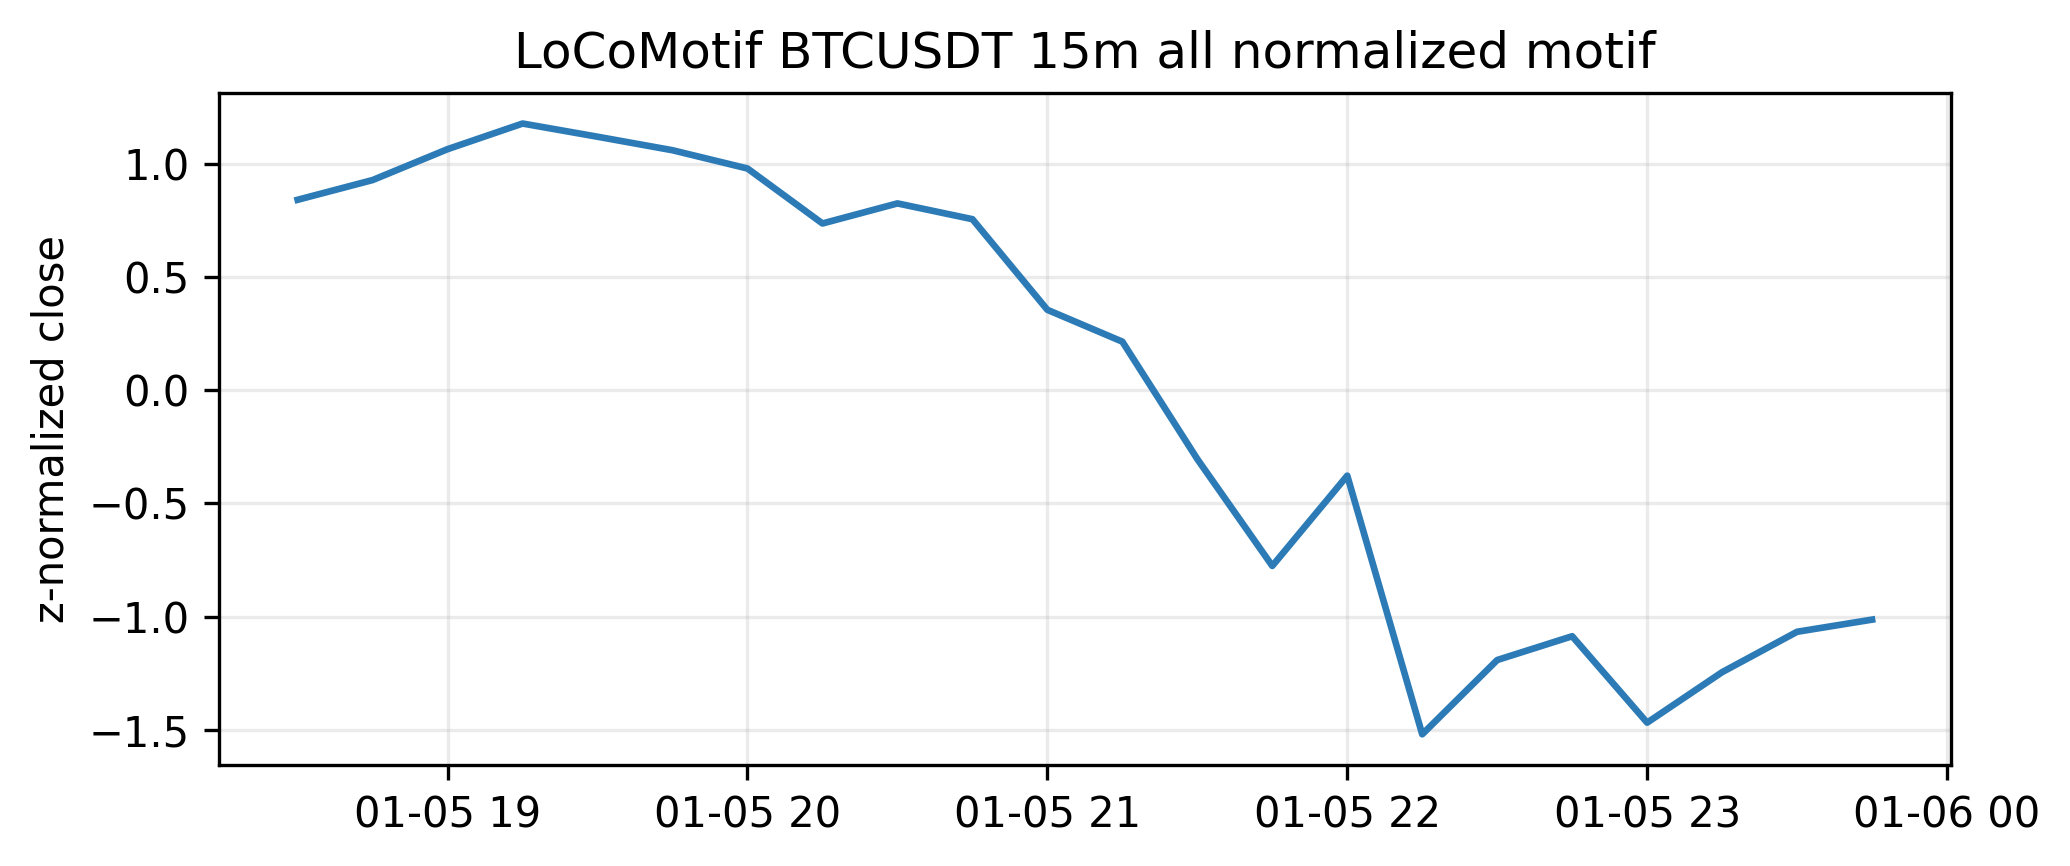
\includegraphics[width=0.9\linewidth]{reports/final_visual_evidence/figures/top_motif_12_locomotif_btcusdt_15m_all_normal_pattern.png}
\caption{top motif 12 locomotif btcusdt 15m all normal pattern. The figure compares real available Matrix Profile and LoCoMotif outputs while preserving object-type differences.}
\end{figure}

\begin{figure}[ht]
\centering
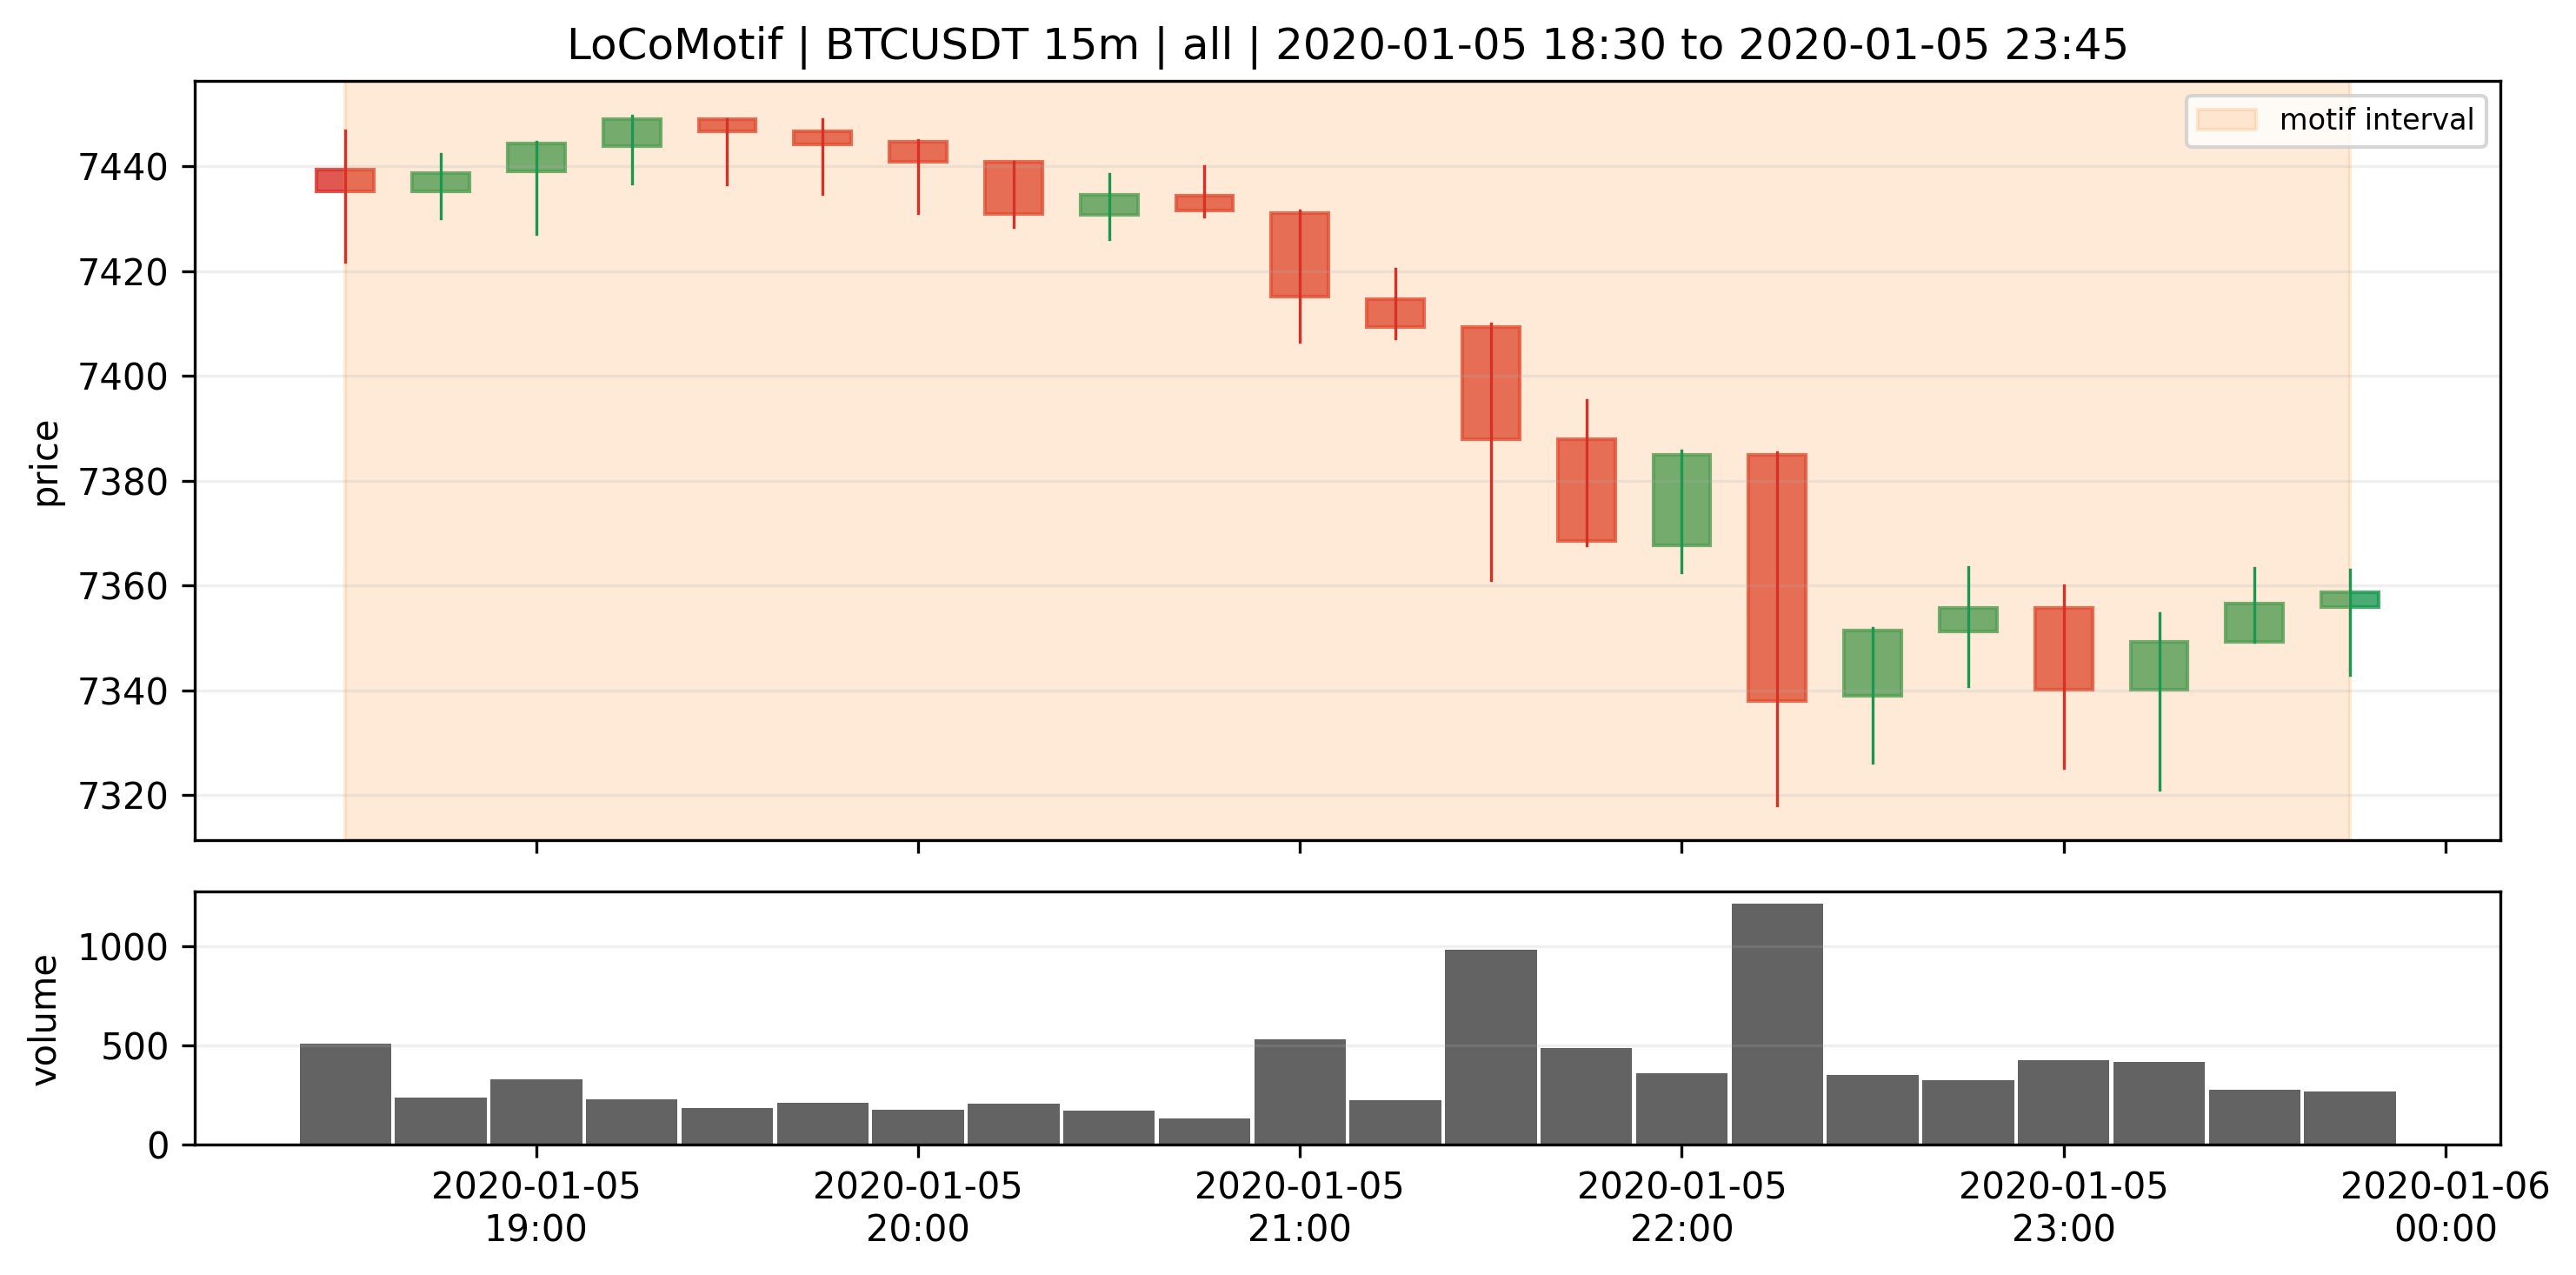
\includegraphics[width=0.9\linewidth]{reports/final_visual_evidence/figures/top_motif_12_locomotif_btcusdt_15m_all_zoom.png}
\caption{top motif 12 locomotif btcusdt 15m all zoom. The figure compares real available Matrix Profile and LoCoMotif outputs while preserving object-type differences.}
\end{figure}

\begin{figure}[ht]
\centering
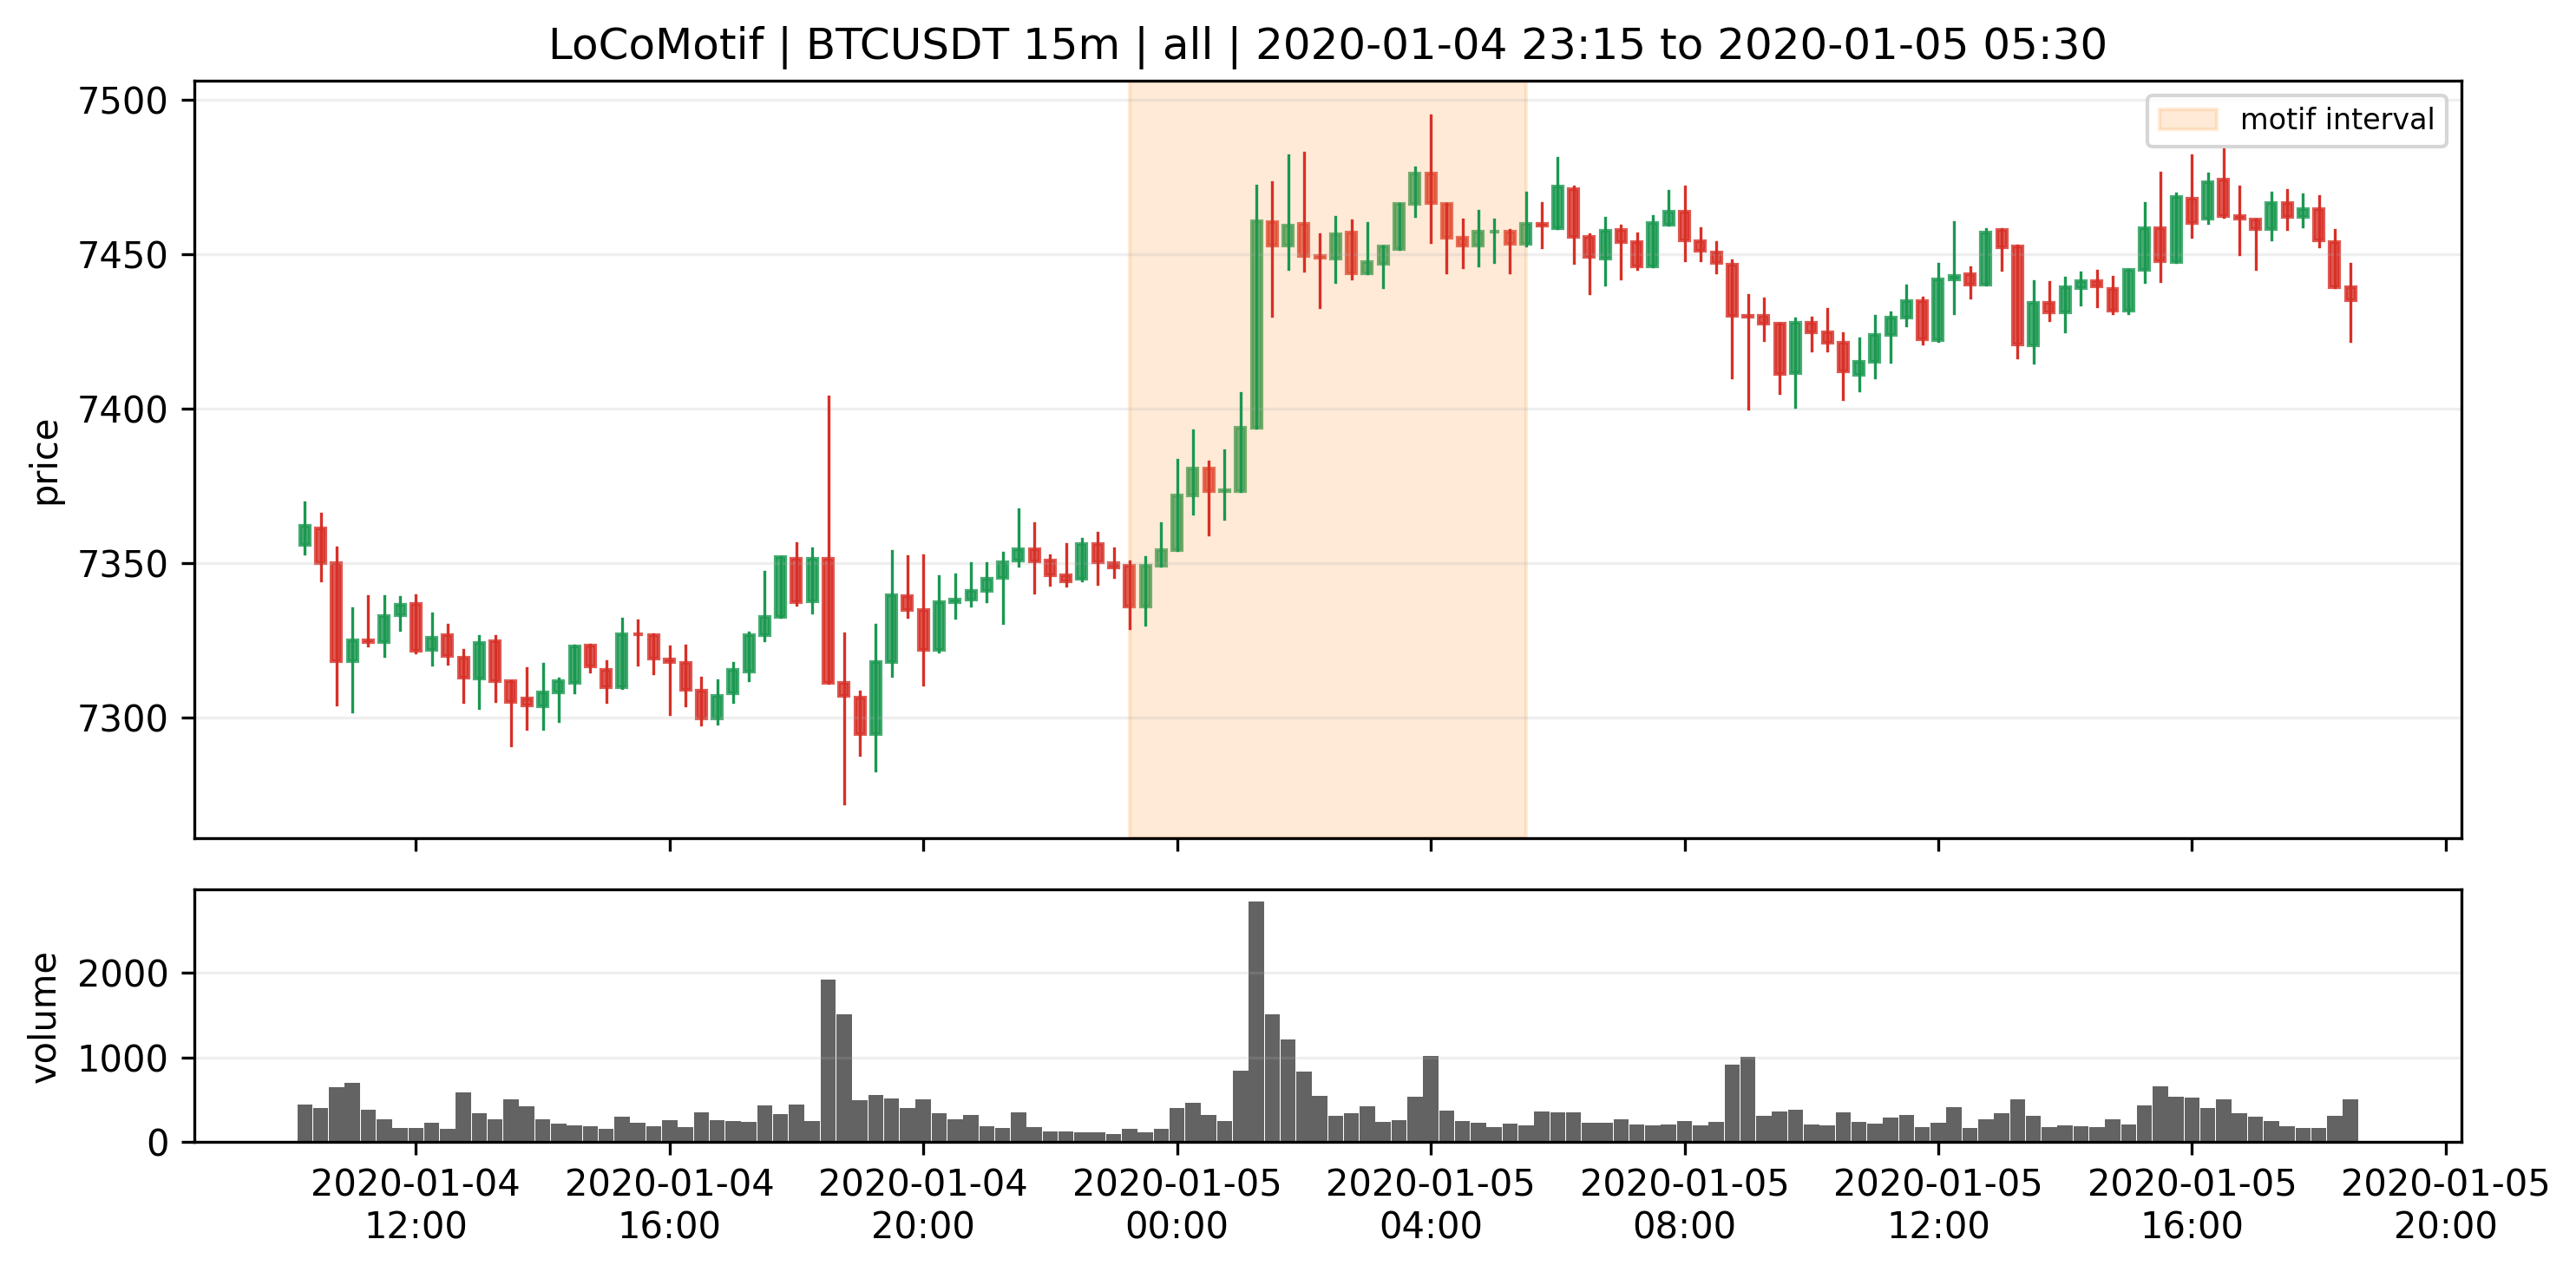
\includegraphics[width=0.9\linewidth]{reports/final_visual_evidence/figures/top_motif_13_locomotif_btcusdt_15m_all_context.png}
\caption{top motif 13 locomotif btcusdt 15m all context. The figure compares real available Matrix Profile and LoCoMotif outputs while preserving object-type differences.}
\end{figure}

\begin{figure}[ht]
\centering
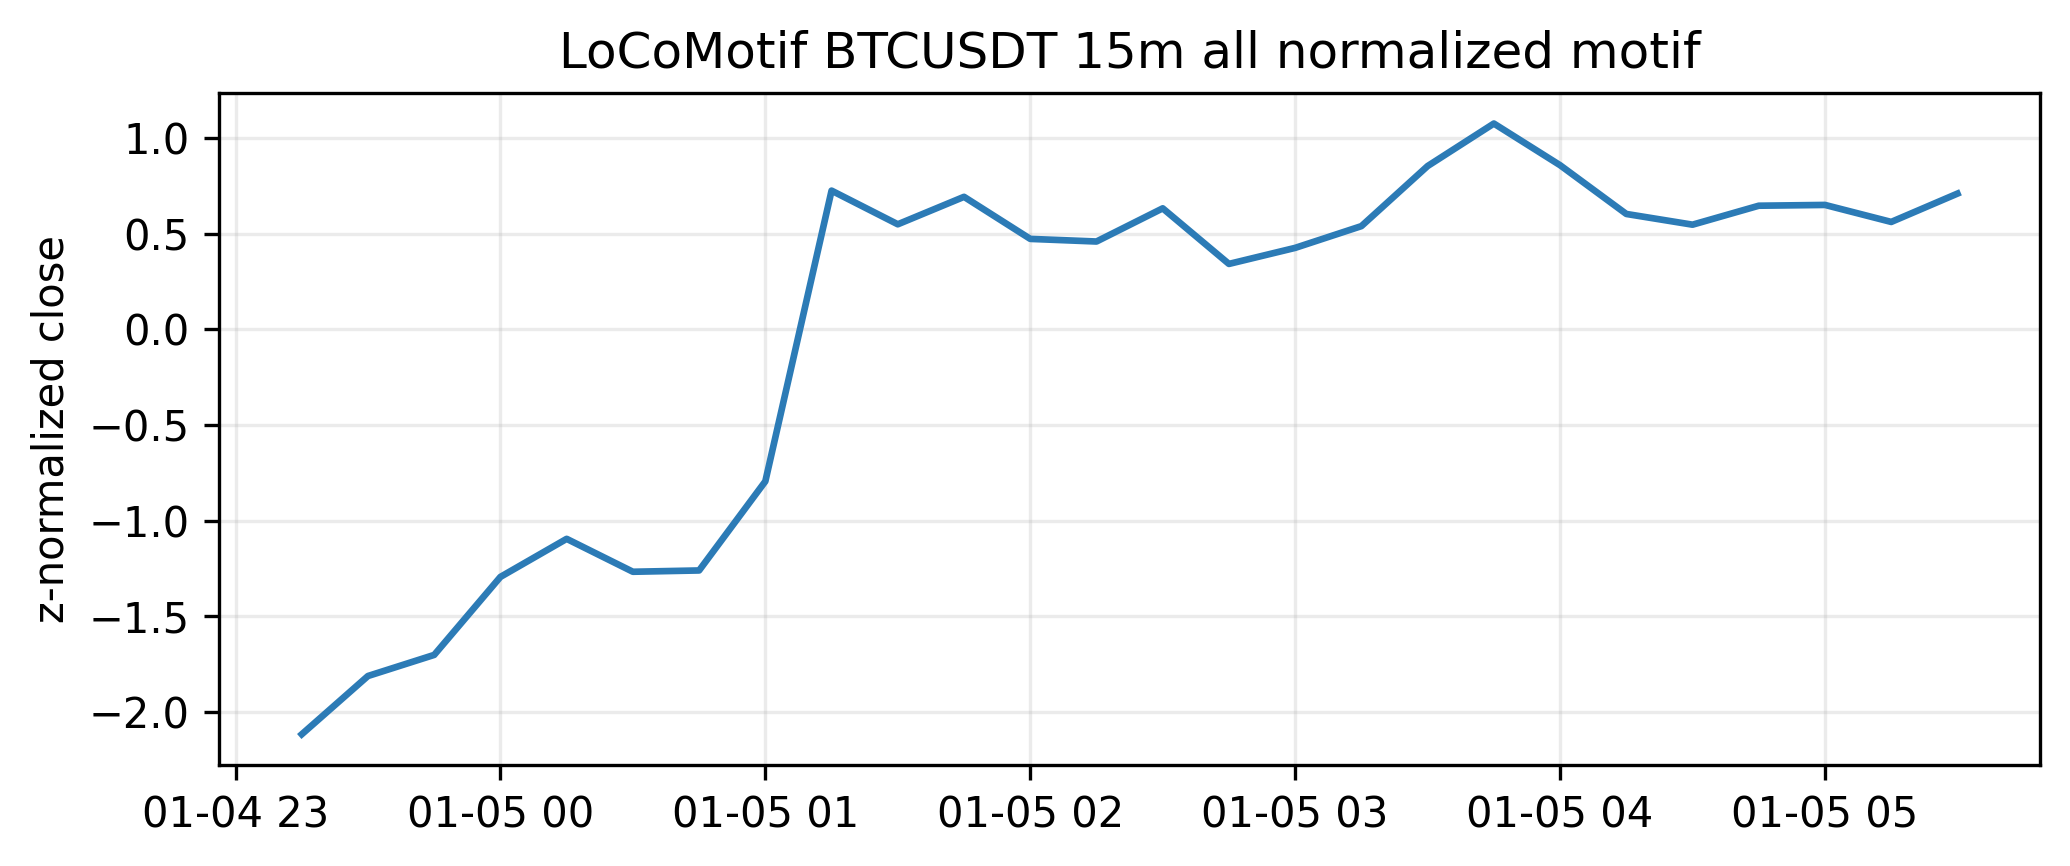
\includegraphics[width=0.9\linewidth]{reports/final_visual_evidence/figures/top_motif_13_locomotif_btcusdt_15m_all_normal_pattern.png}
\caption{top motif 13 locomotif btcusdt 15m all normal pattern. The figure compares real available Matrix Profile and LoCoMotif outputs while preserving object-type differences.}
\end{figure}

\begin{figure}[ht]
\centering
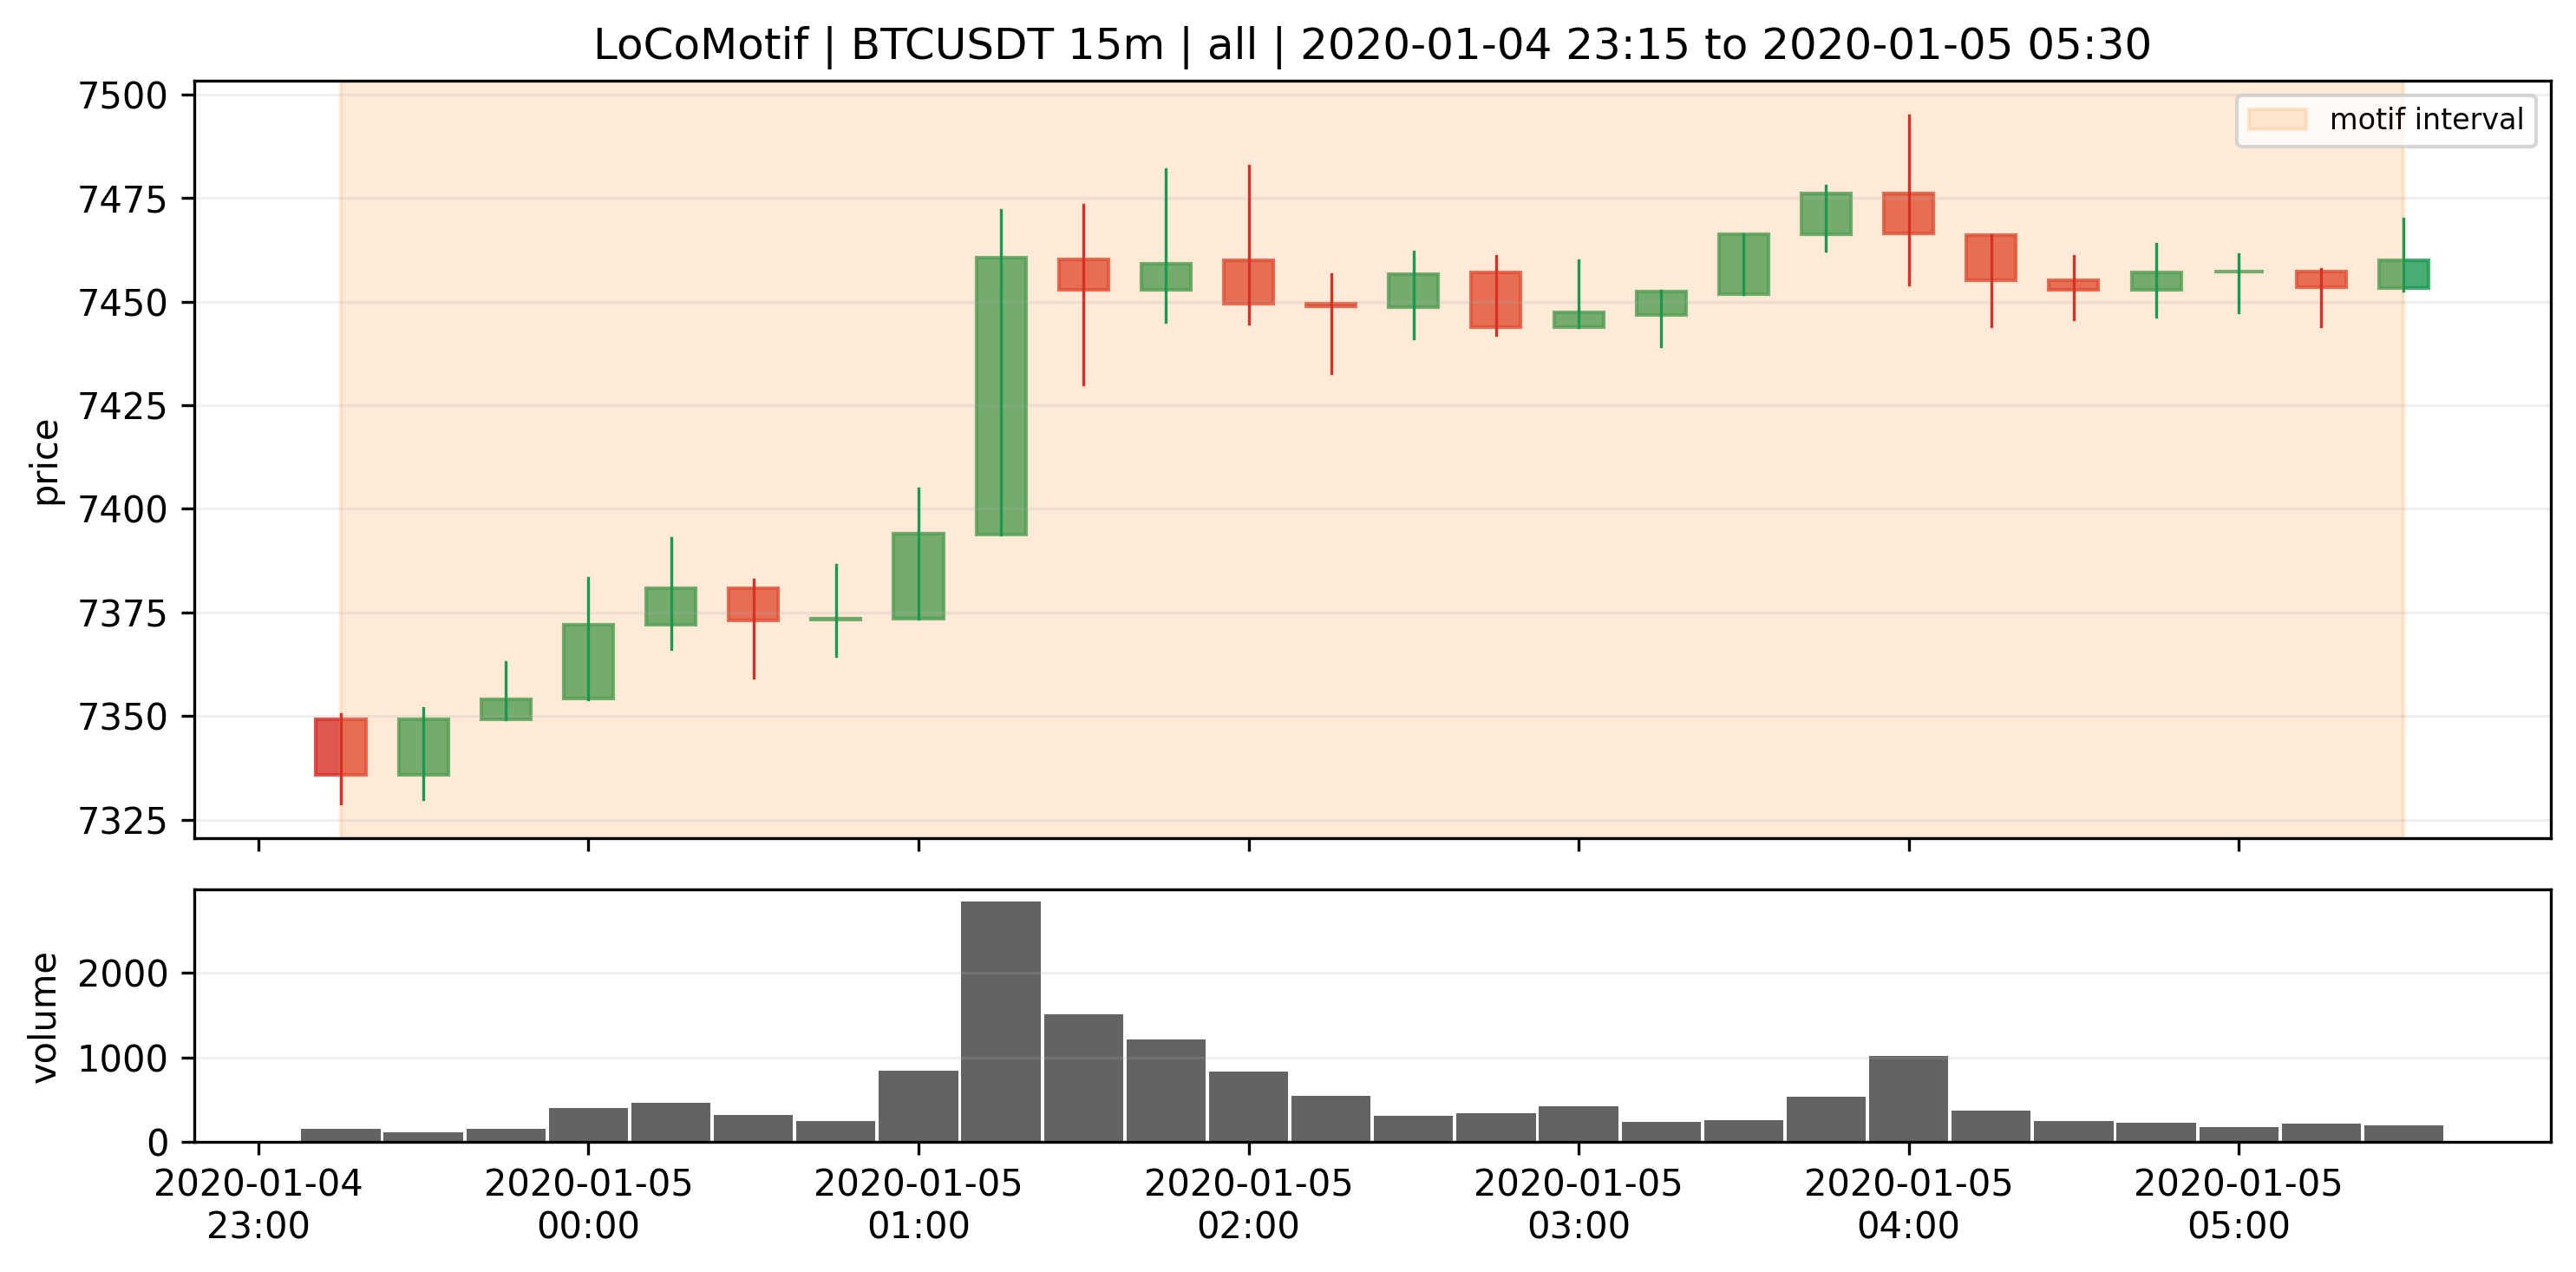
\includegraphics[width=0.9\linewidth]{reports/final_visual_evidence/figures/top_motif_13_locomotif_btcusdt_15m_all_zoom.png}
\caption{top motif 13 locomotif btcusdt 15m all zoom. The figure compares real available Matrix Profile and LoCoMotif outputs while preserving object-type differences.}
\end{figure}

\begin{figure}[ht]
\centering
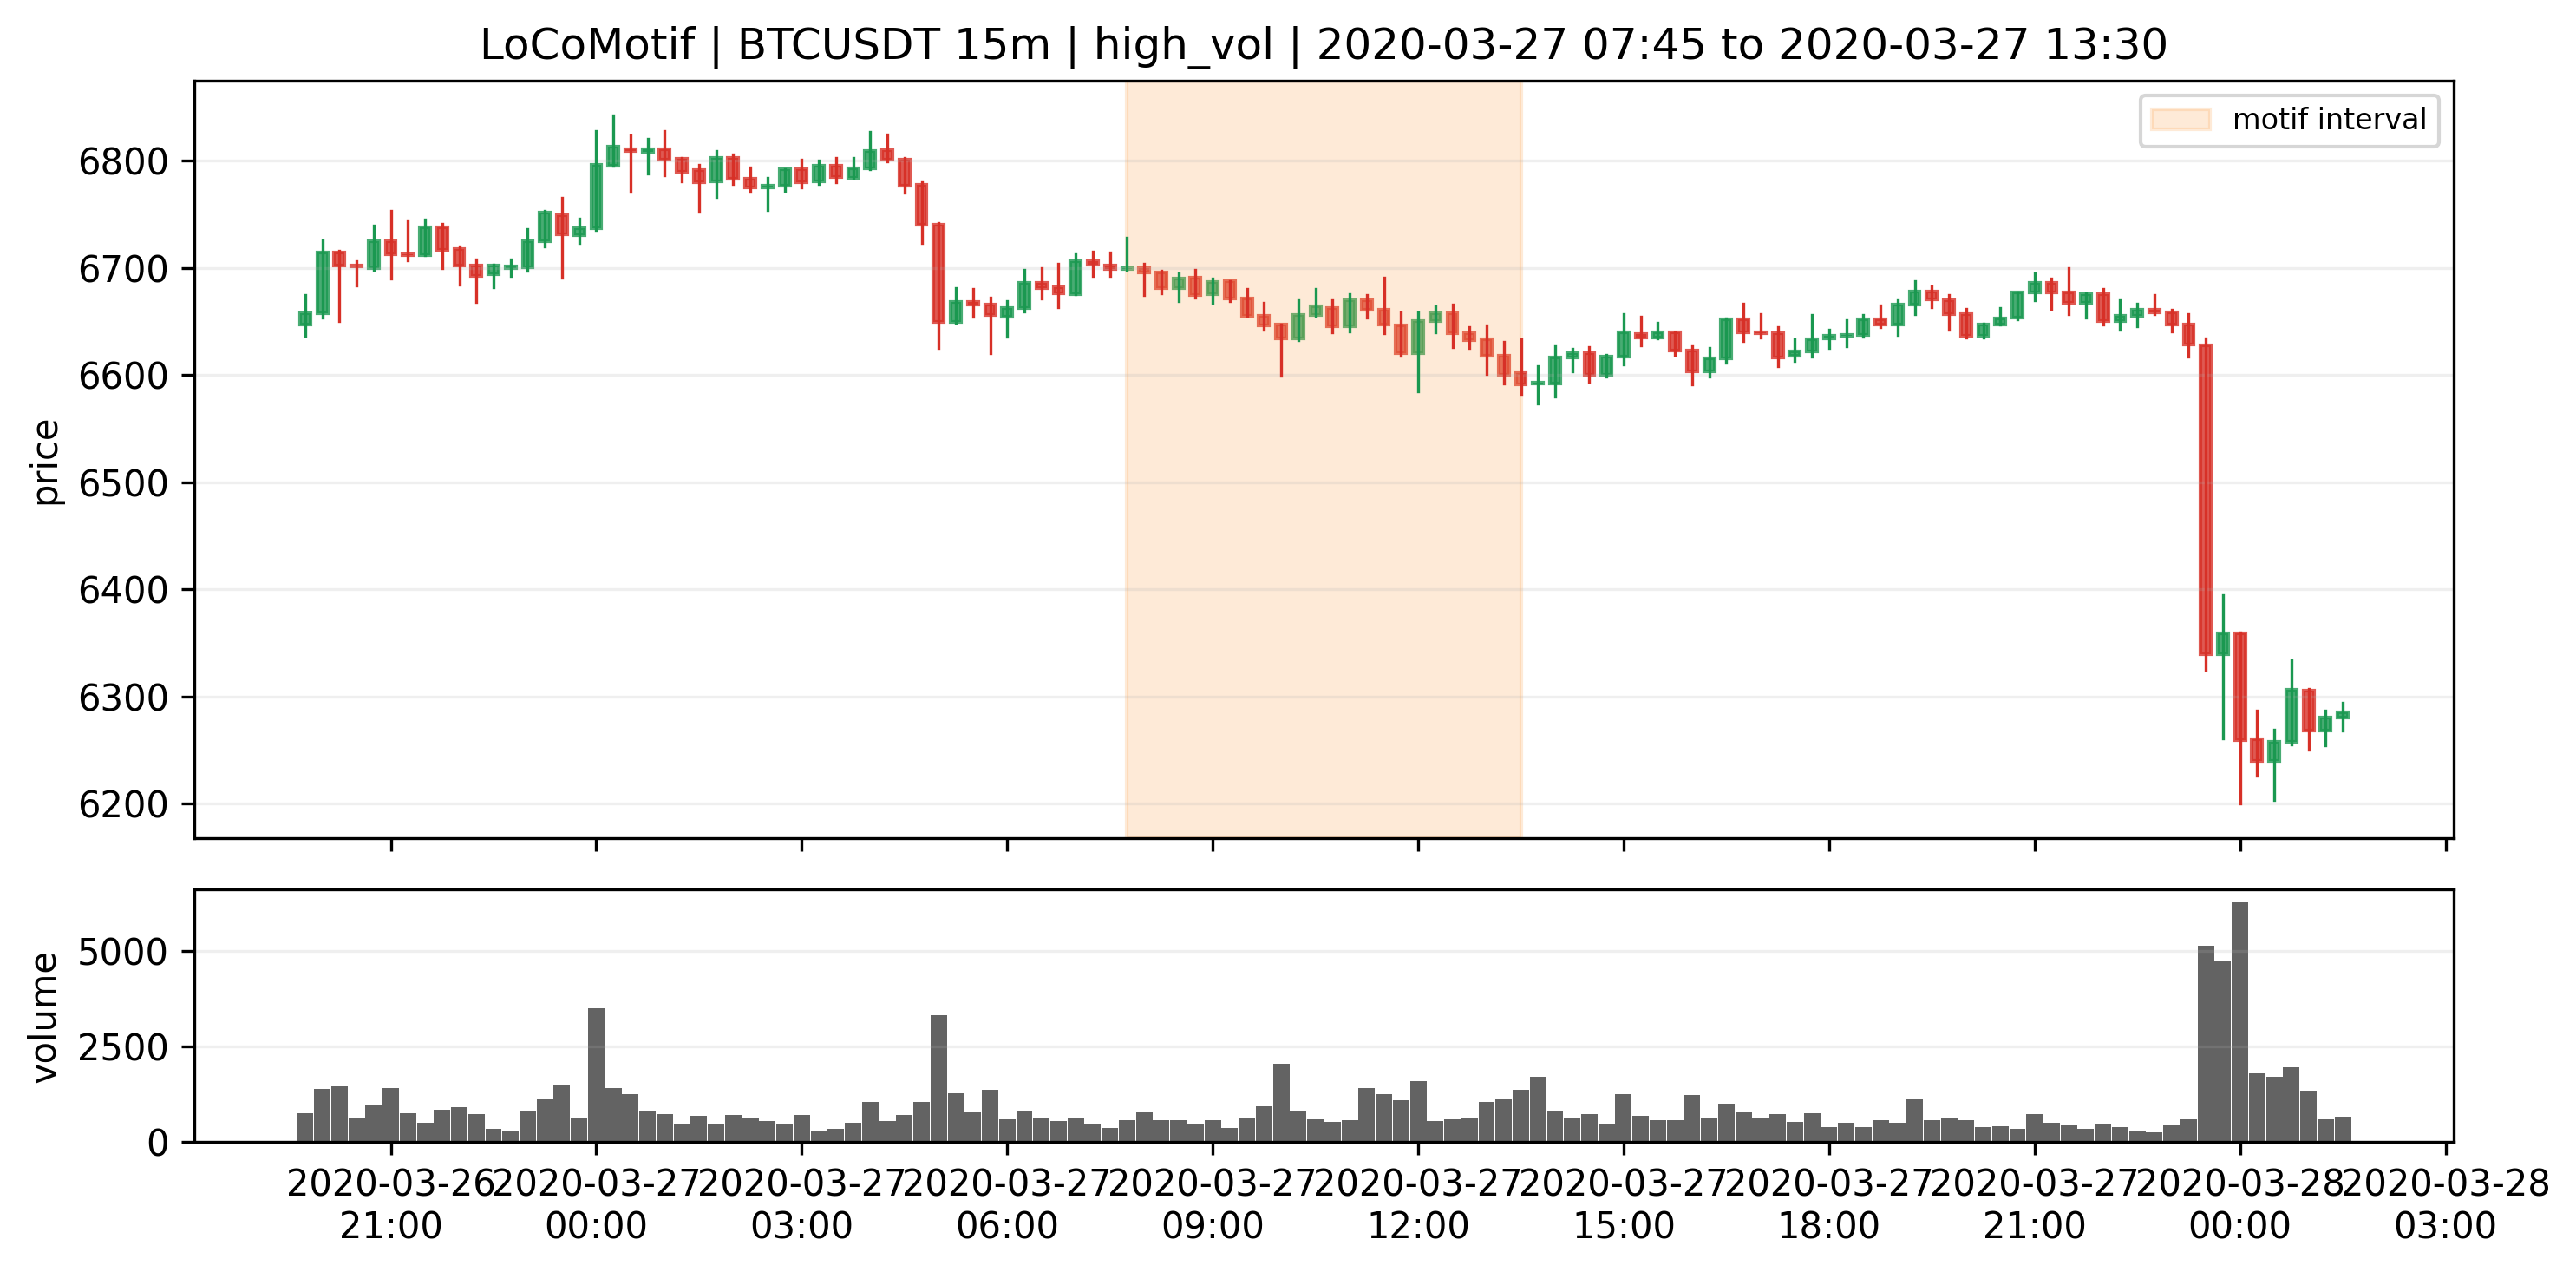
\includegraphics[width=0.9\linewidth]{reports/final_visual_evidence/figures/top_motif_14_locomotif_btcusdt_15m_high_vol_context.png}
\caption{top motif 14 locomotif btcusdt 15m high vol context. The figure compares real available Matrix Profile and LoCoMotif outputs while preserving object-type differences.}
\end{figure}

\begin{figure}[ht]
\centering
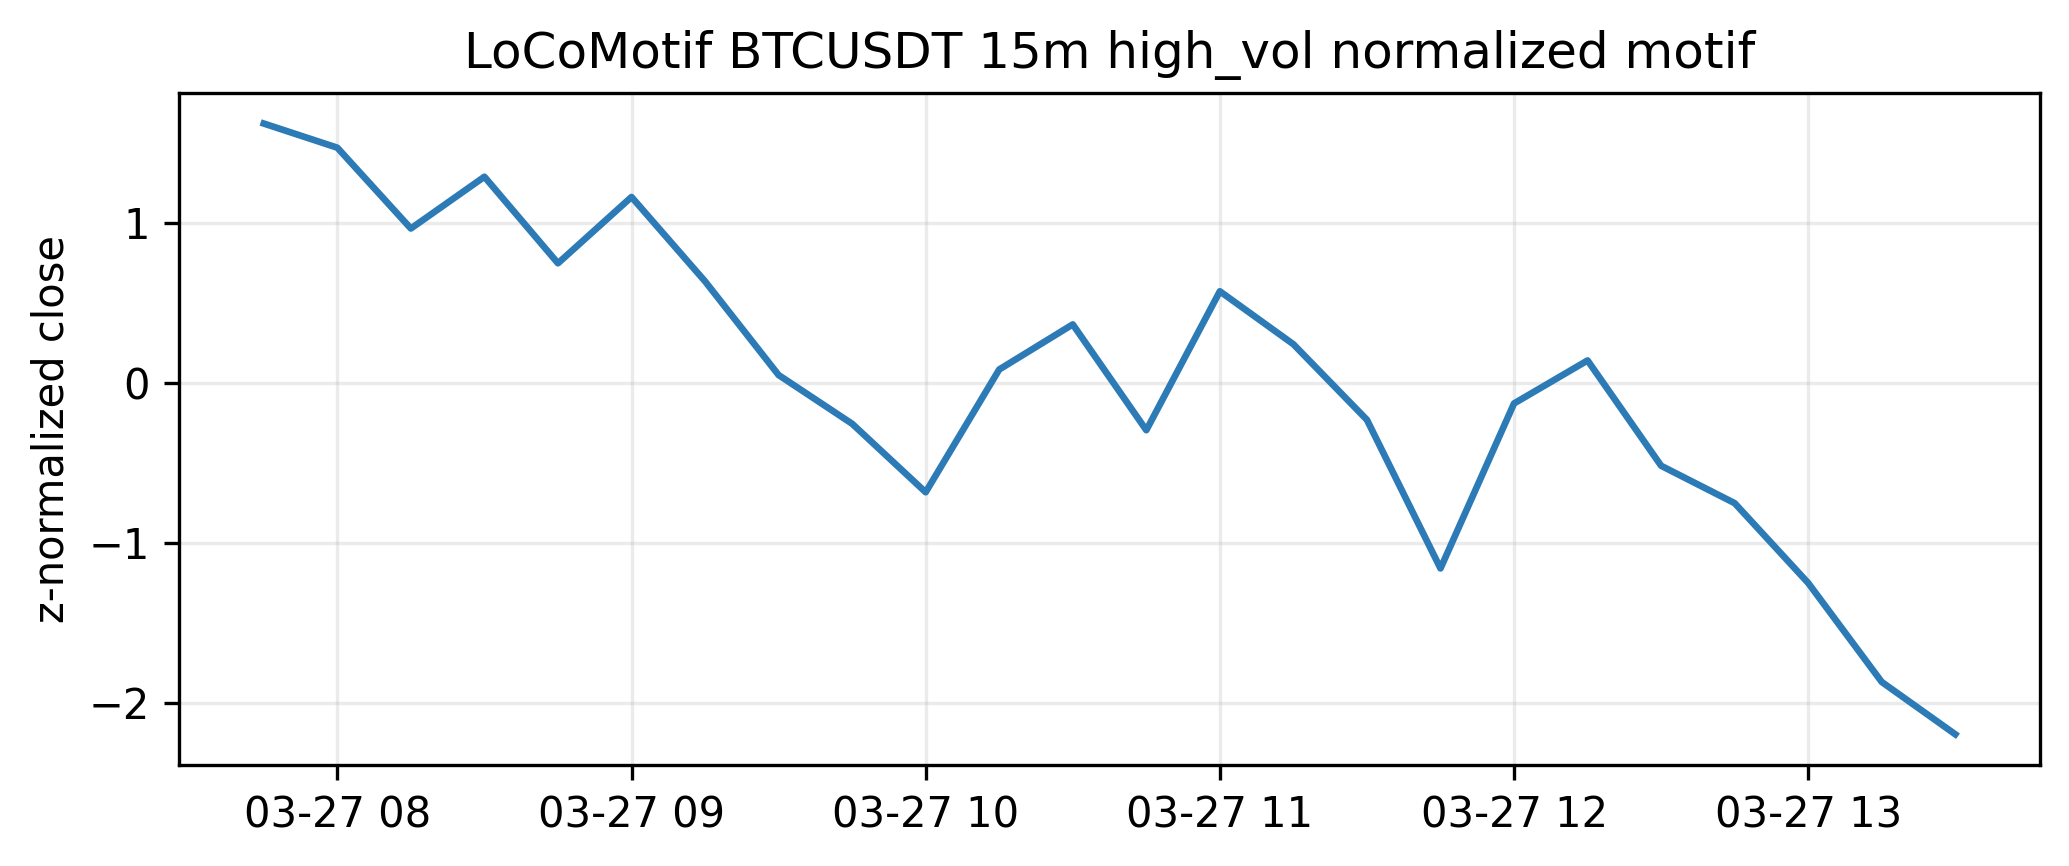
\includegraphics[width=0.9\linewidth]{reports/final_visual_evidence/figures/top_motif_14_locomotif_btcusdt_15m_high_vol_normal_pattern.png}
\caption{top motif 14 locomotif btcusdt 15m high vol normal pattern. The figure compares real available Matrix Profile and LoCoMotif outputs while preserving object-type differences.}
\end{figure}

\begin{figure}[ht]
\centering
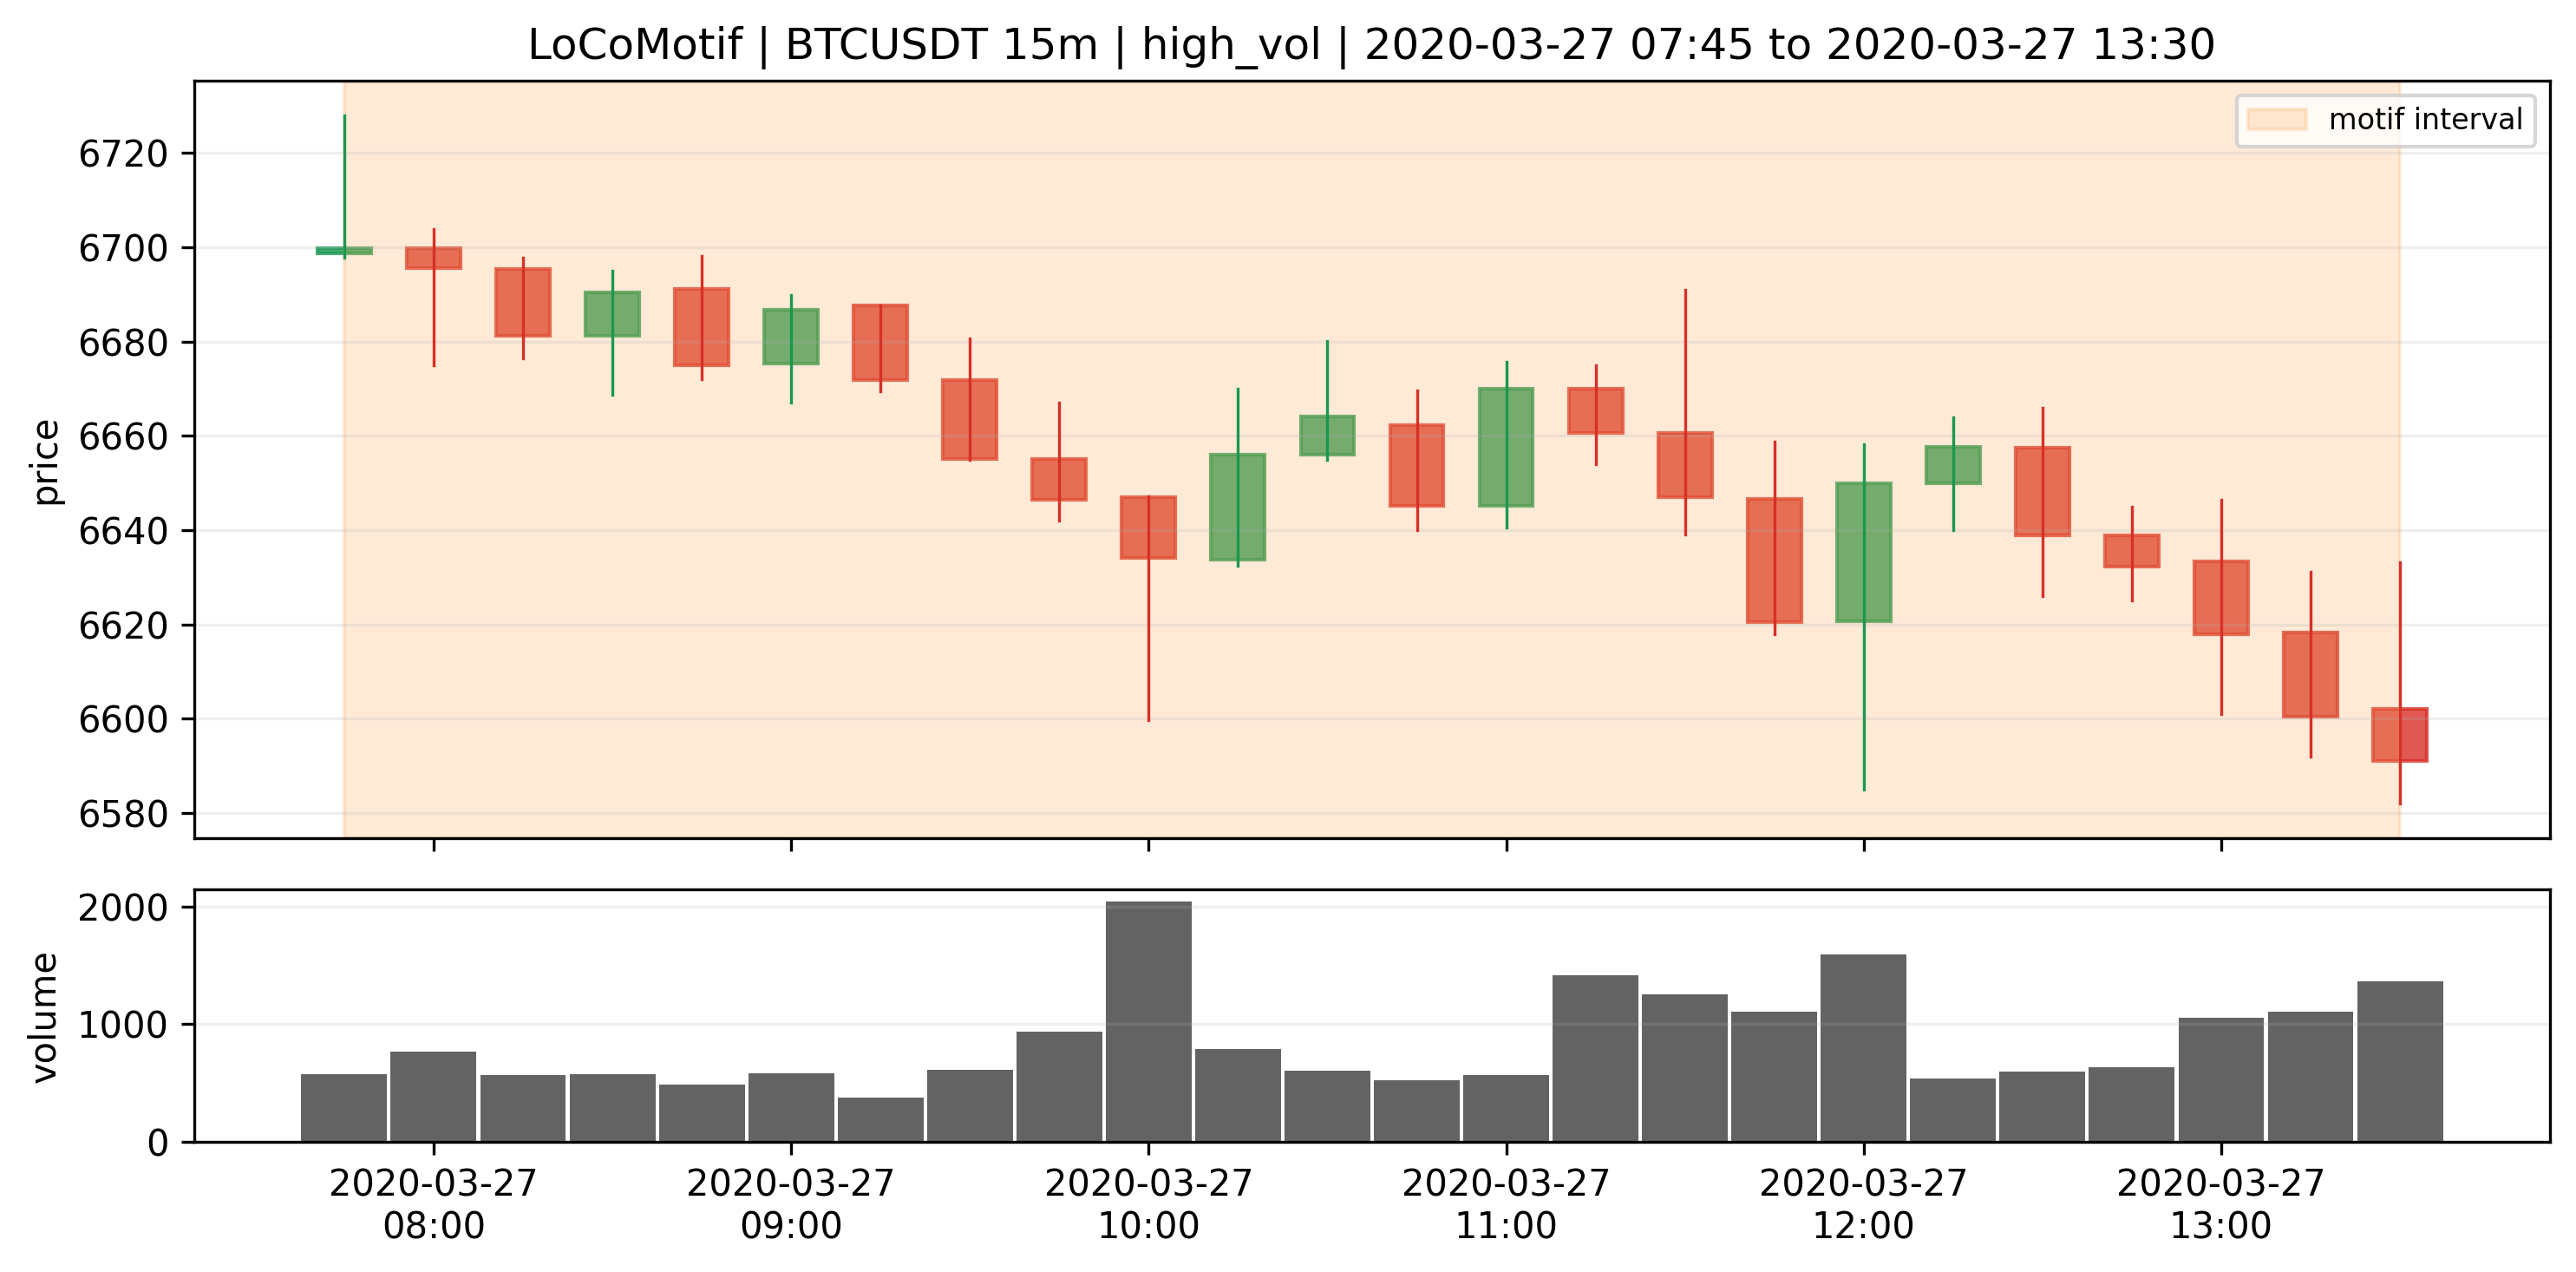
\includegraphics[width=0.9\linewidth]{reports/final_visual_evidence/figures/top_motif_14_locomotif_btcusdt_15m_high_vol_zoom.png}
\caption{top motif 14 locomotif btcusdt 15m high vol zoom. The figure compares real available Matrix Profile and LoCoMotif outputs while preserving object-type differences.}
\end{figure}

\begin{figure}[ht]
\centering
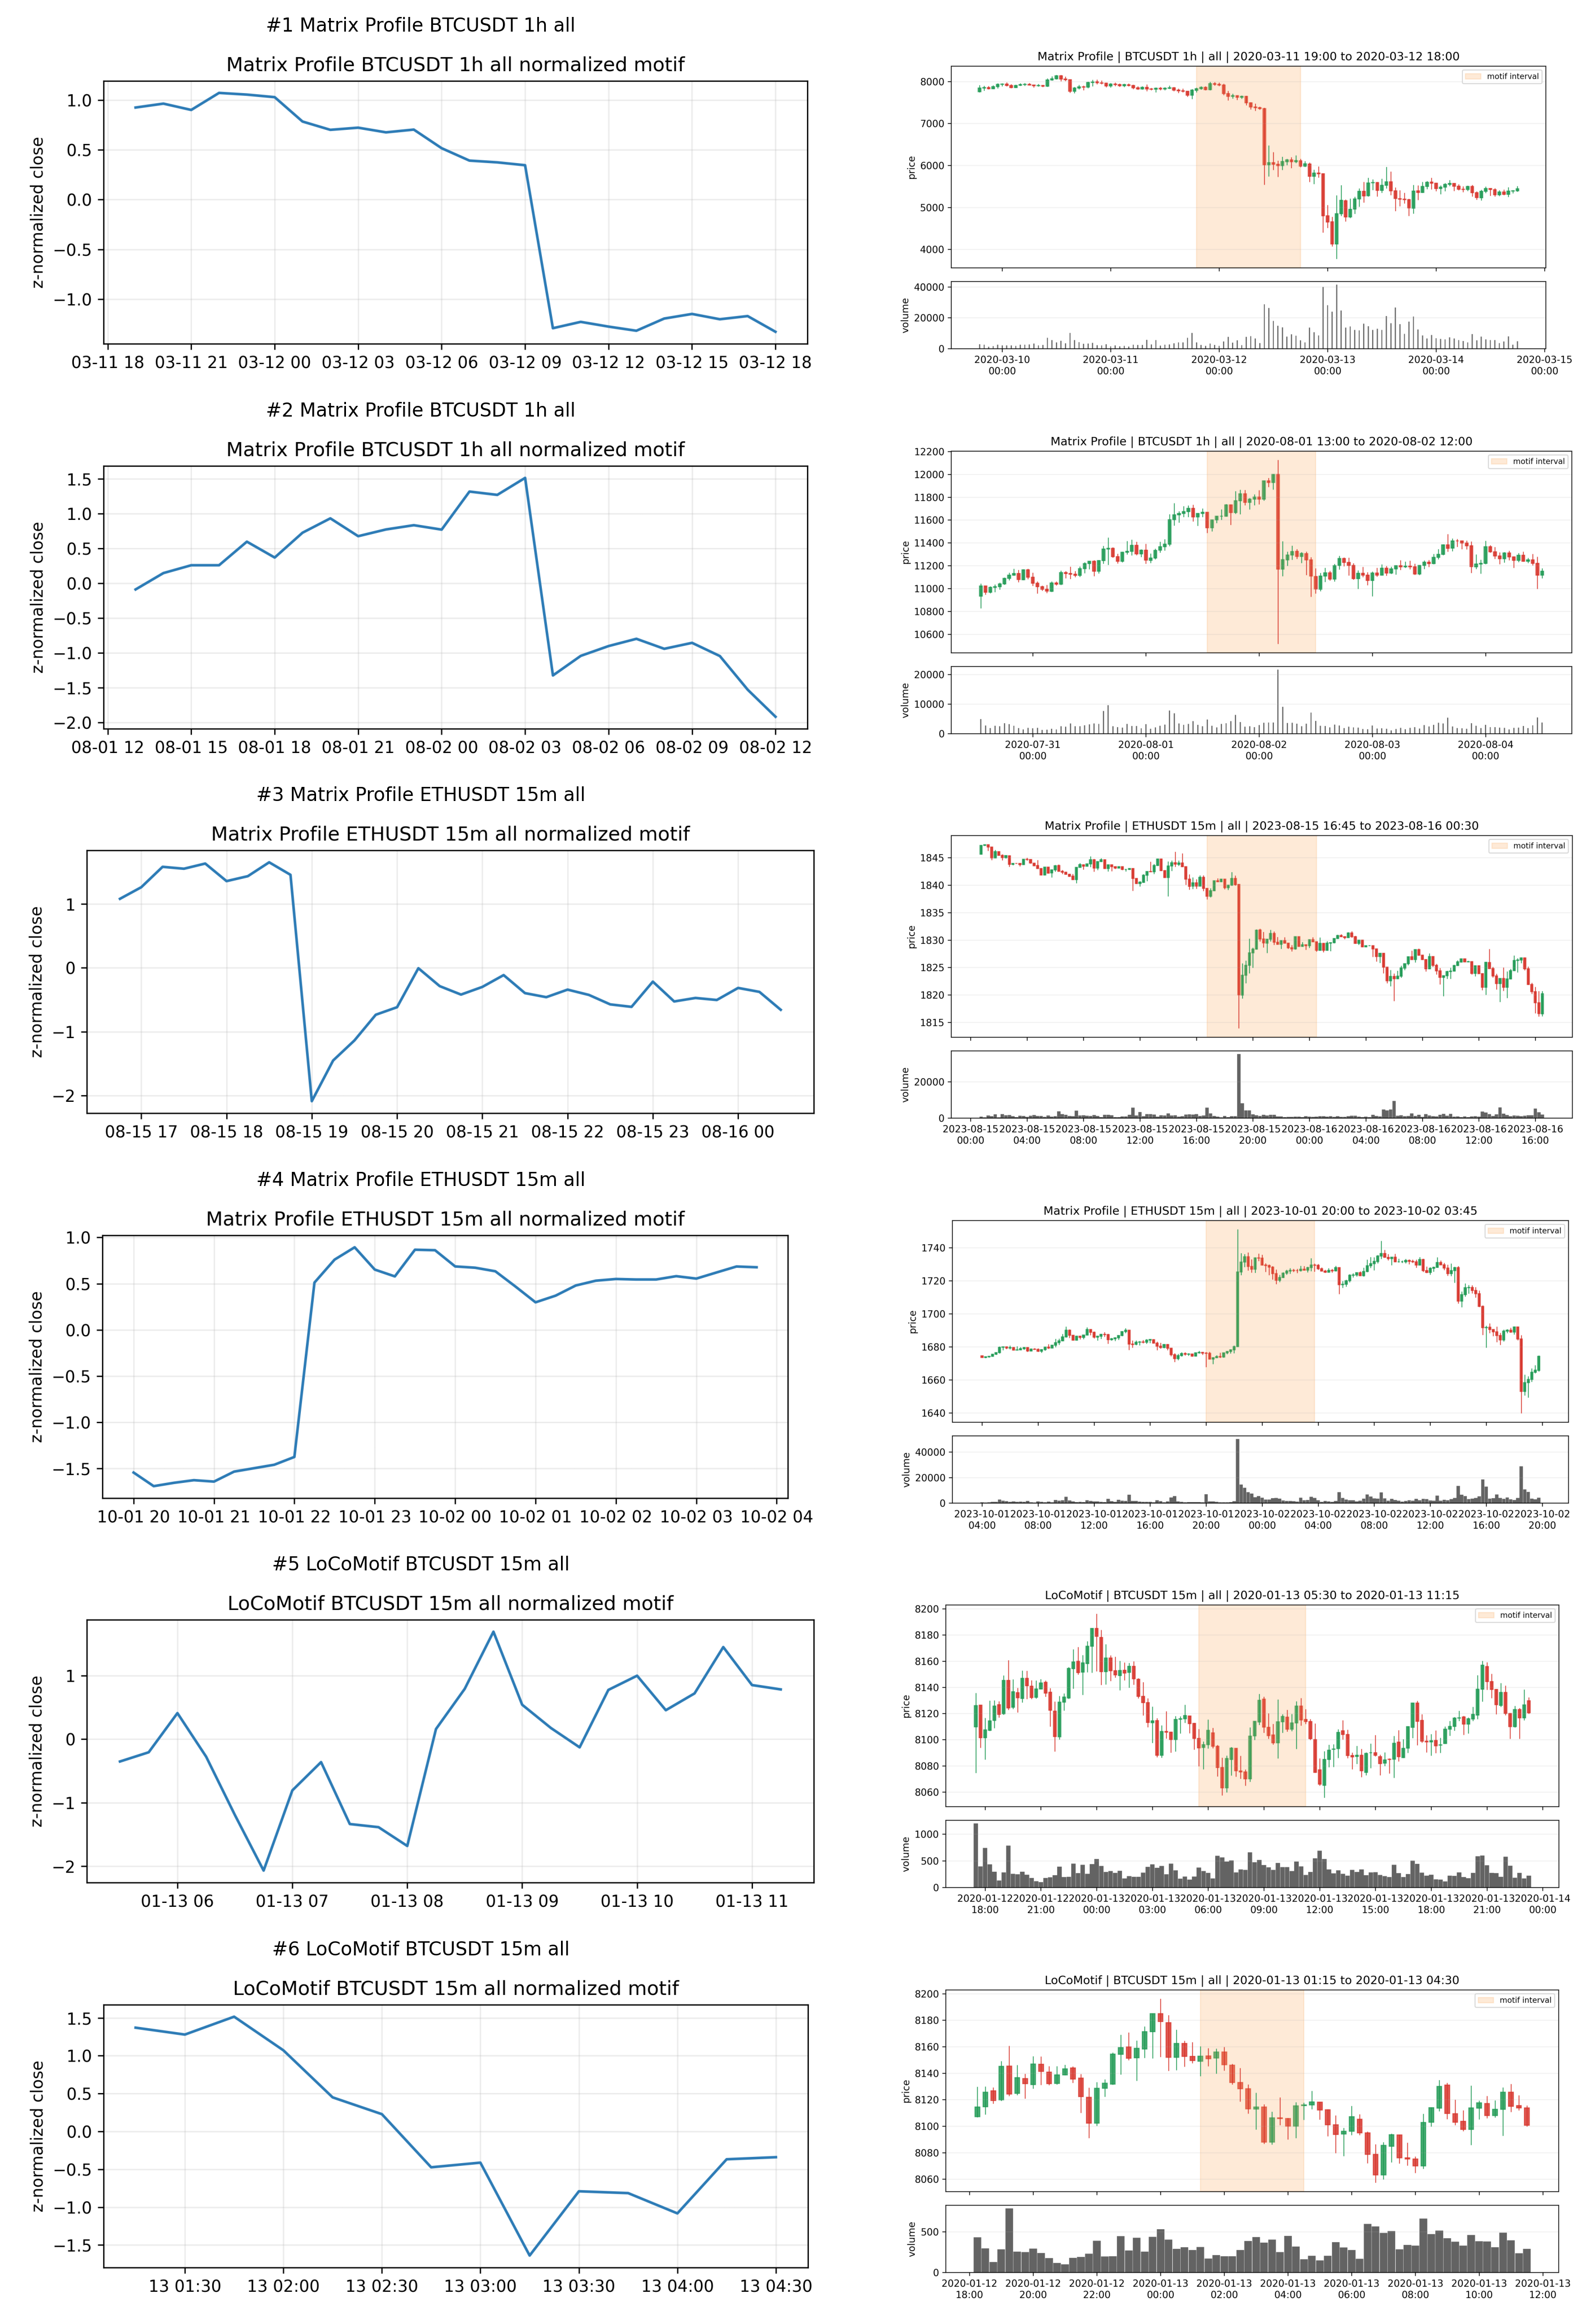
\includegraphics[width=0.9\linewidth]{reports/final_visual_evidence/figures/top_motif_gallery_page_01.png}
\caption{top motif gallery page 01. The shaded interval marks the discovered motif occurrence in original price context.}
\end{figure}

\begin{figure}[ht]
\centering
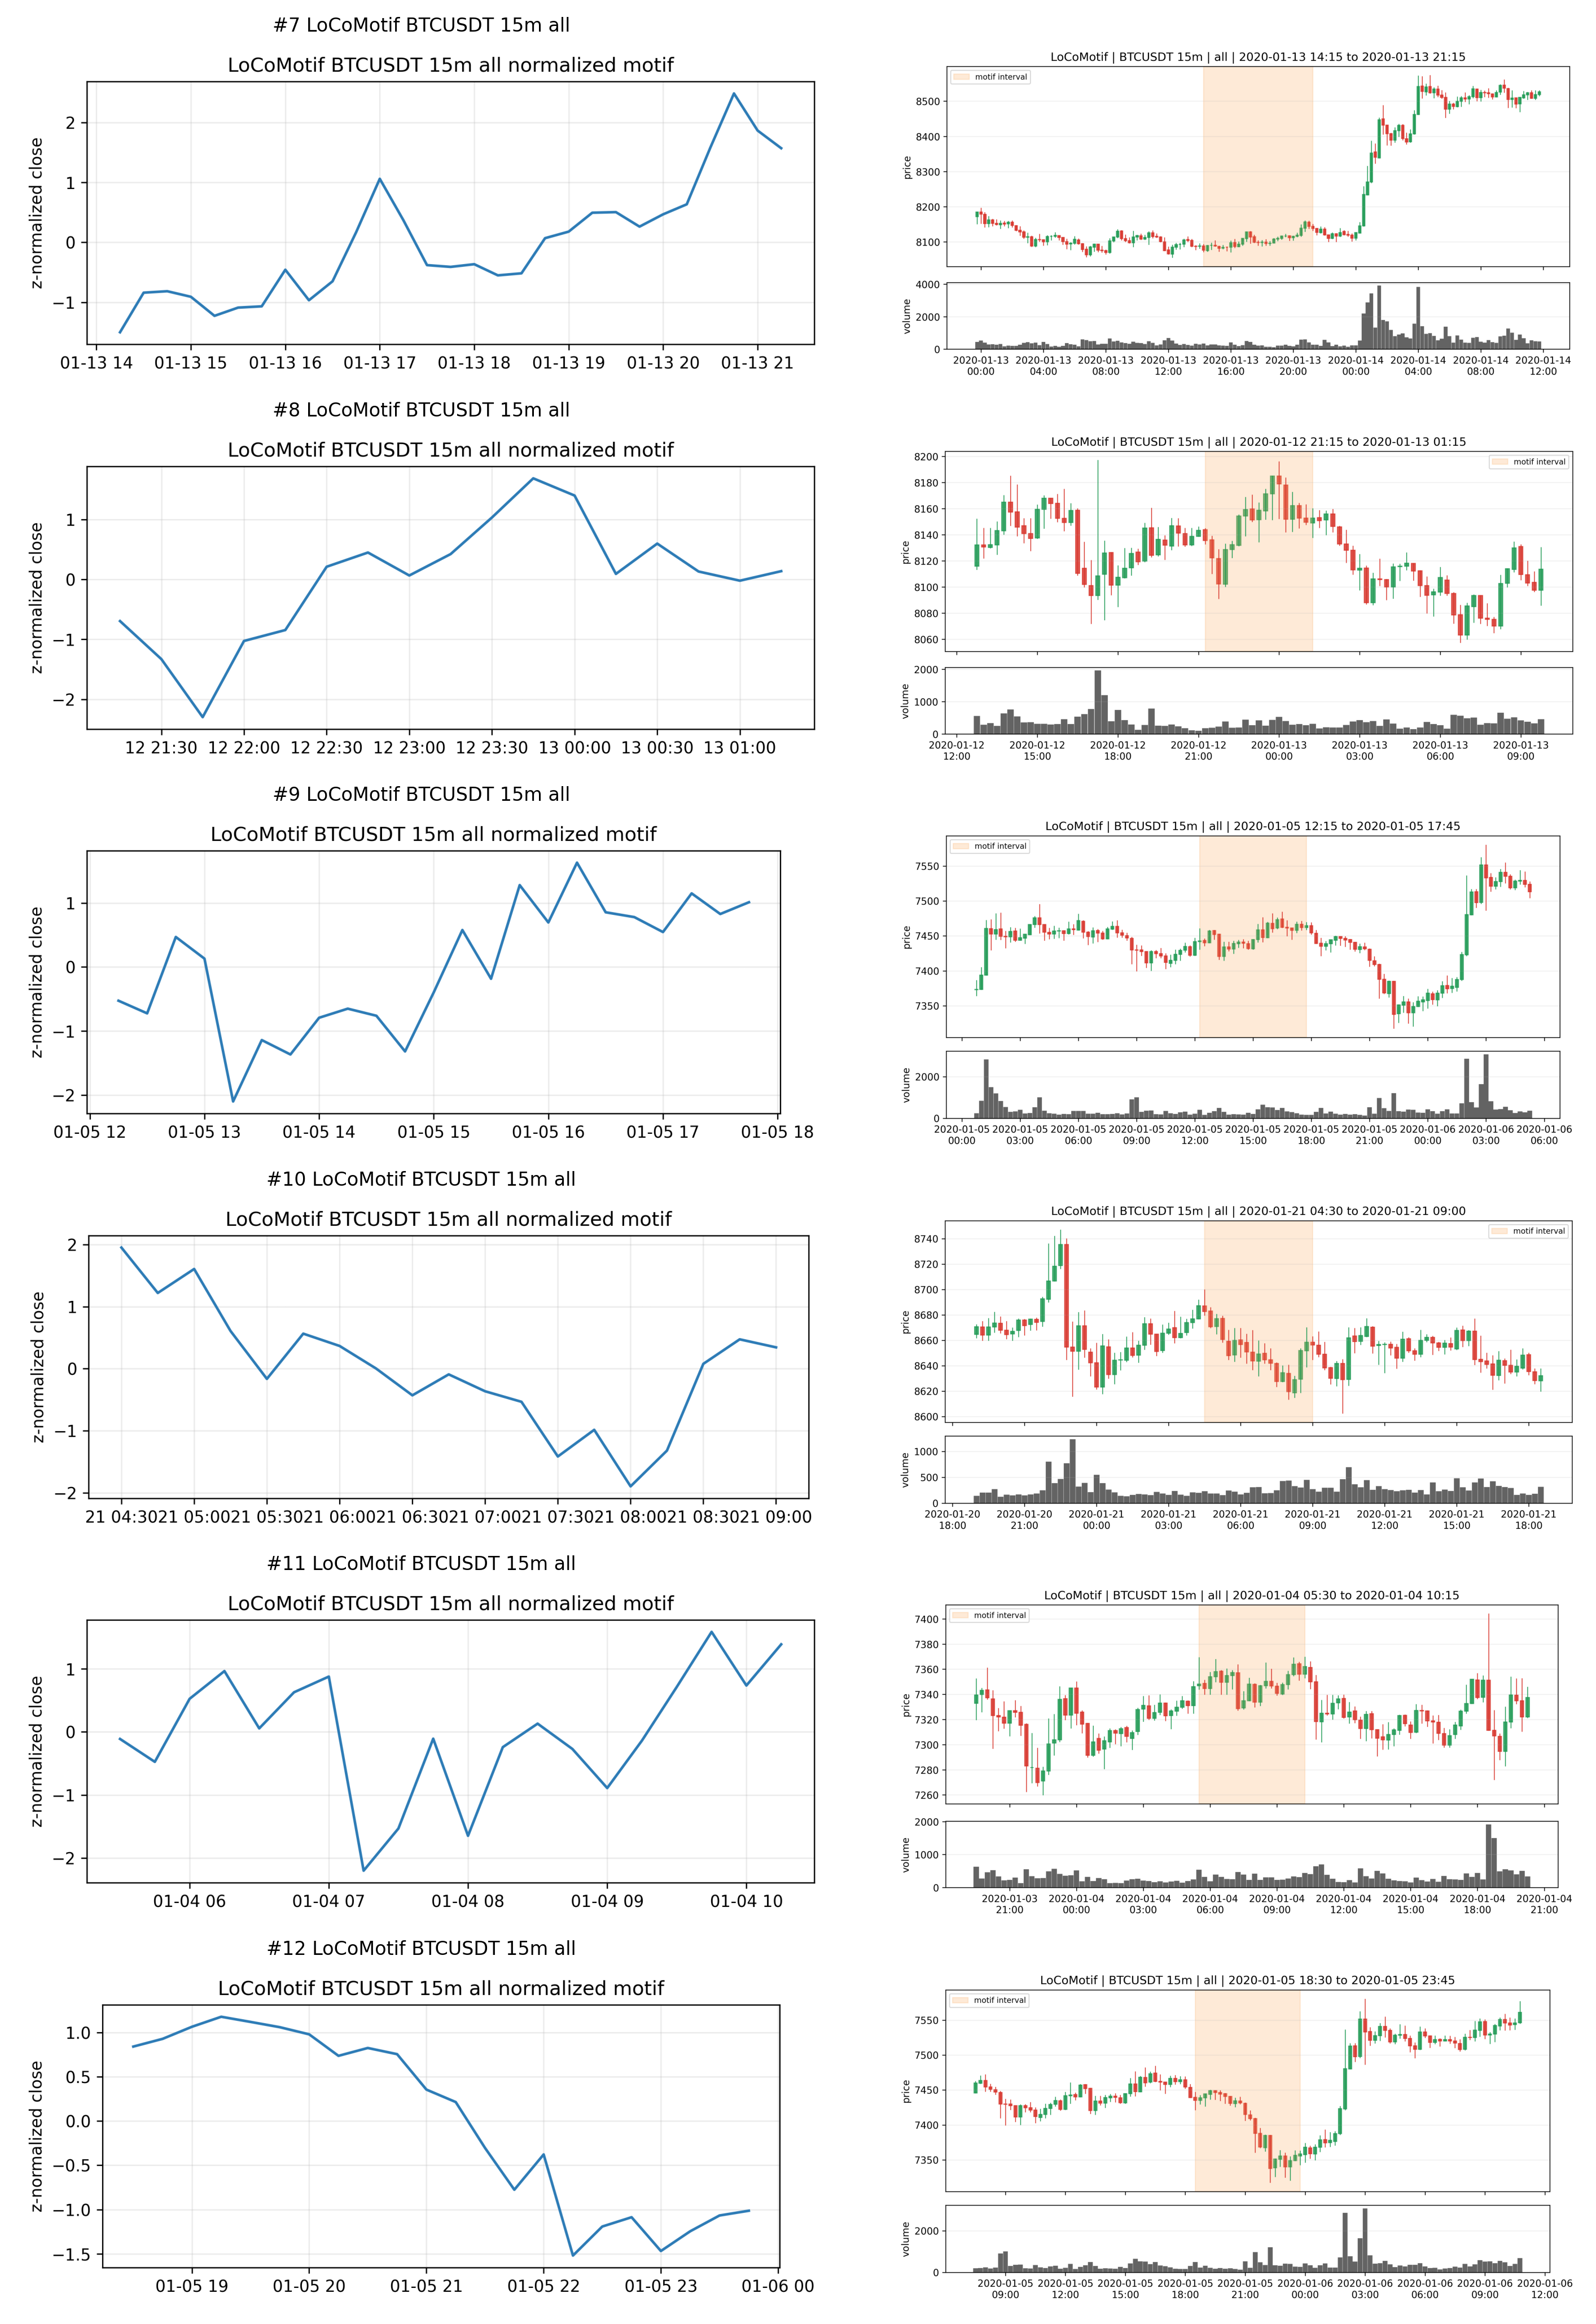
\includegraphics[width=0.9\linewidth]{reports/final_visual_evidence/figures/top_motif_gallery_page_02.png}
\caption{top motif gallery page 02. The shaded interval marks the discovered motif occurrence in original price context.}
\end{figure}

\begin{figure}[ht]
\centering
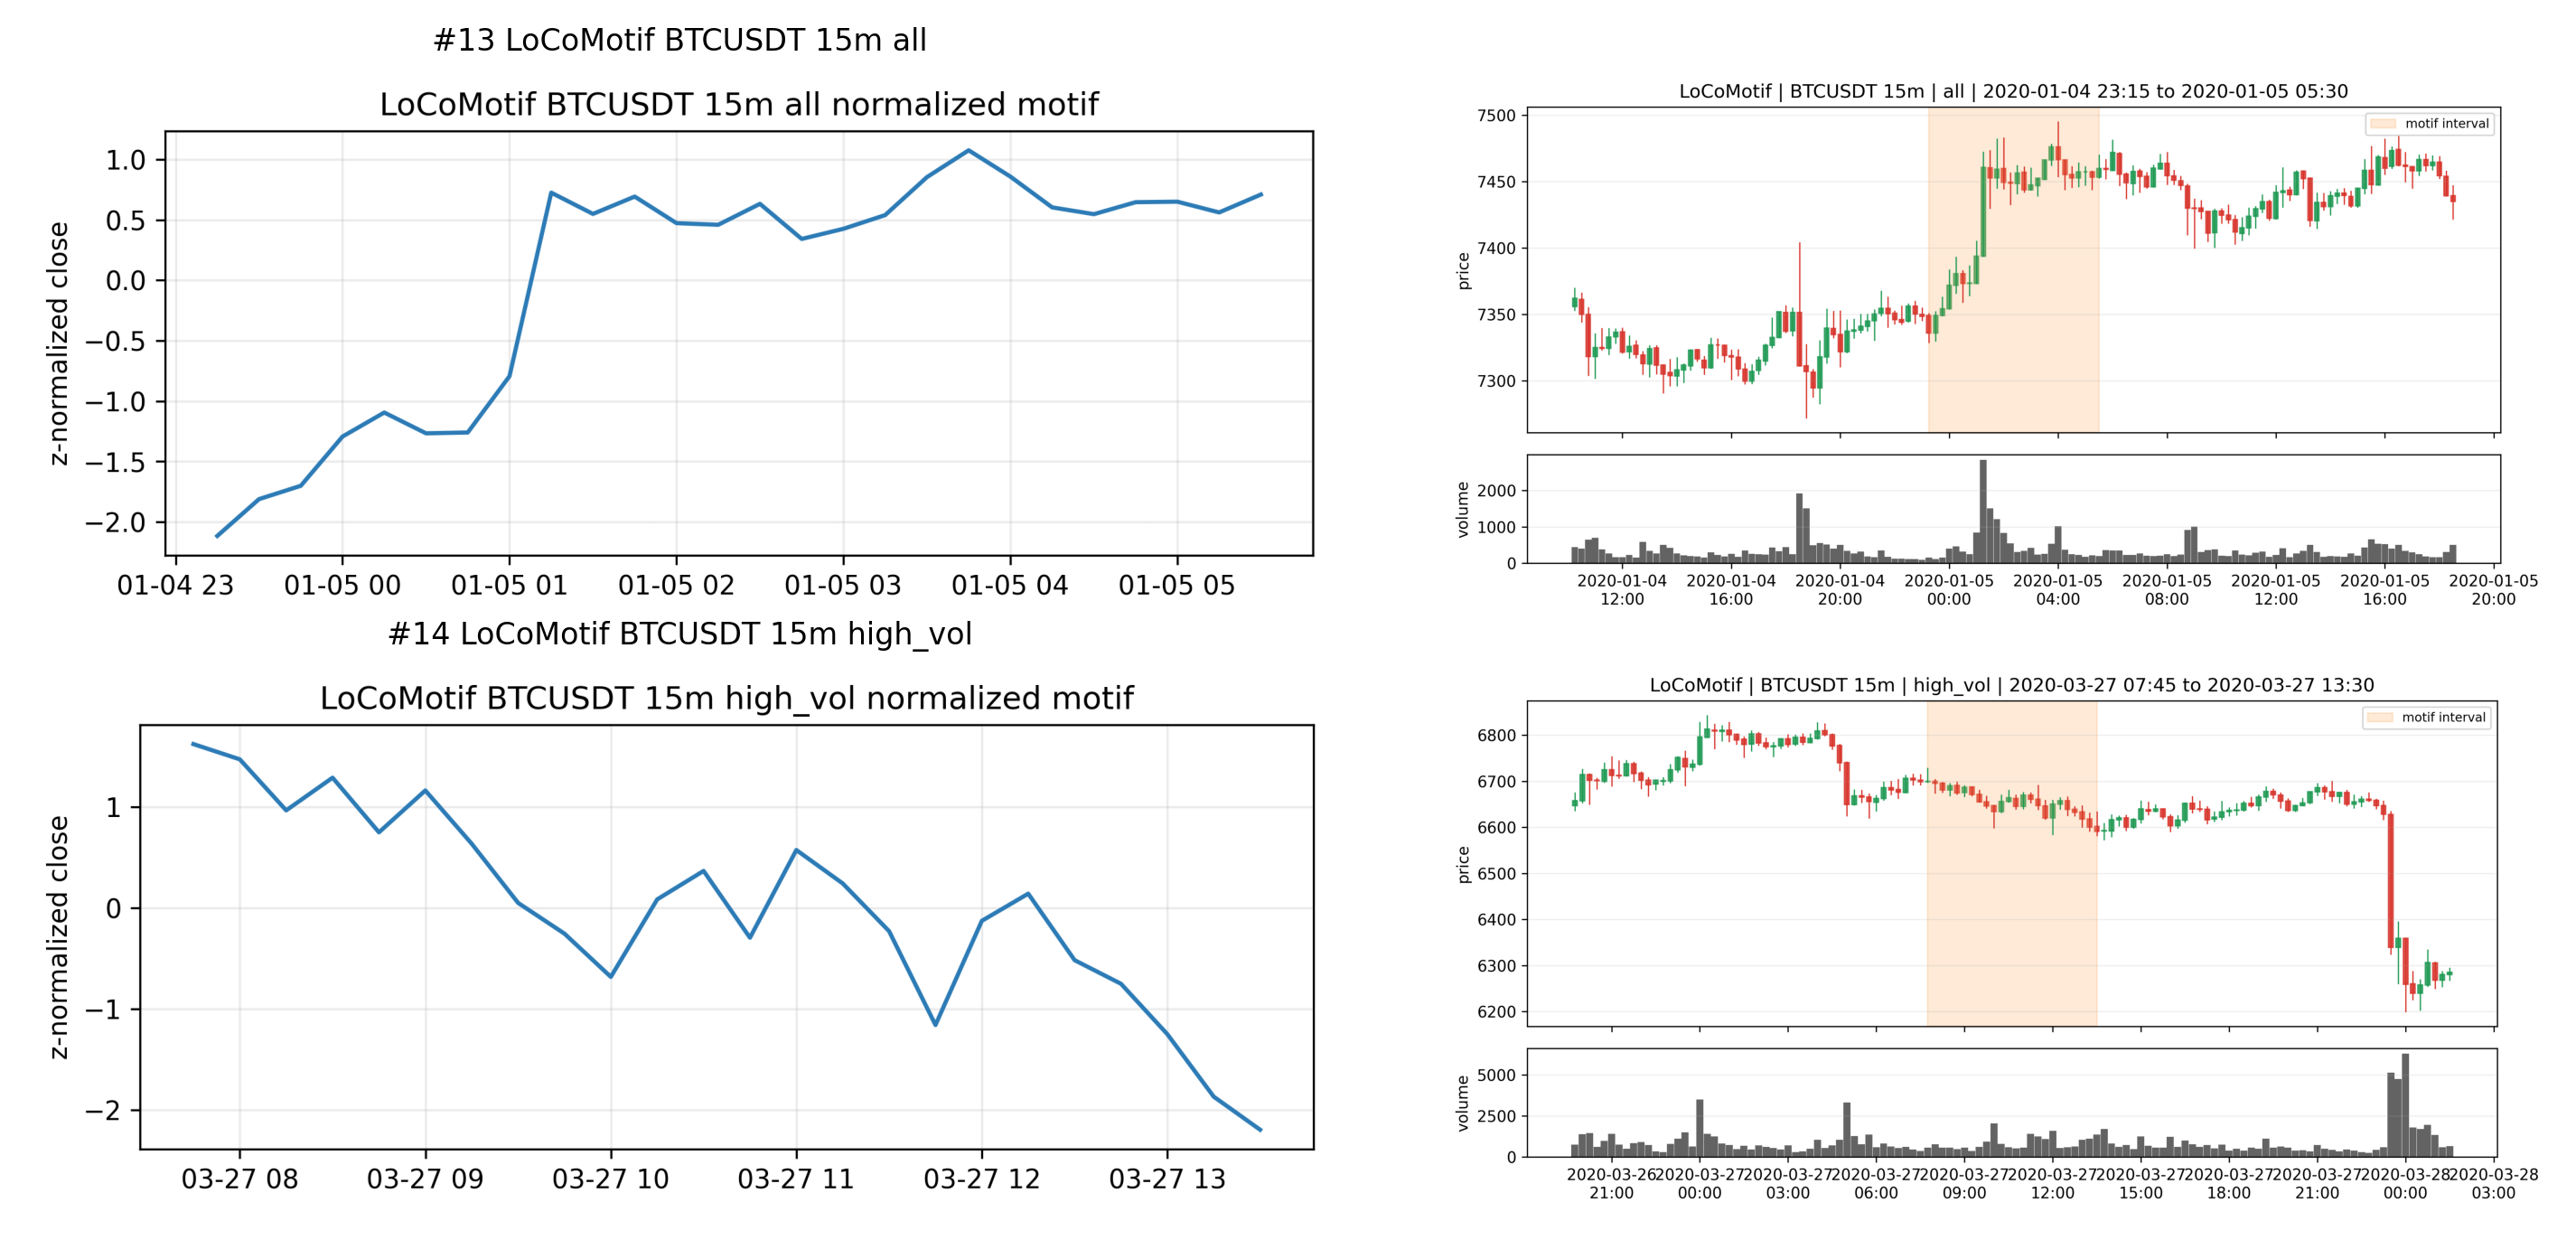
\includegraphics[width=0.9\linewidth]{reports/final_visual_evidence/figures/top_motif_gallery_page_03.png}
\caption{top motif gallery page 03. The shaded interval marks the discovered motif occurrence in original price context.}
\end{figure}

\begin{figure}[ht]
\centering
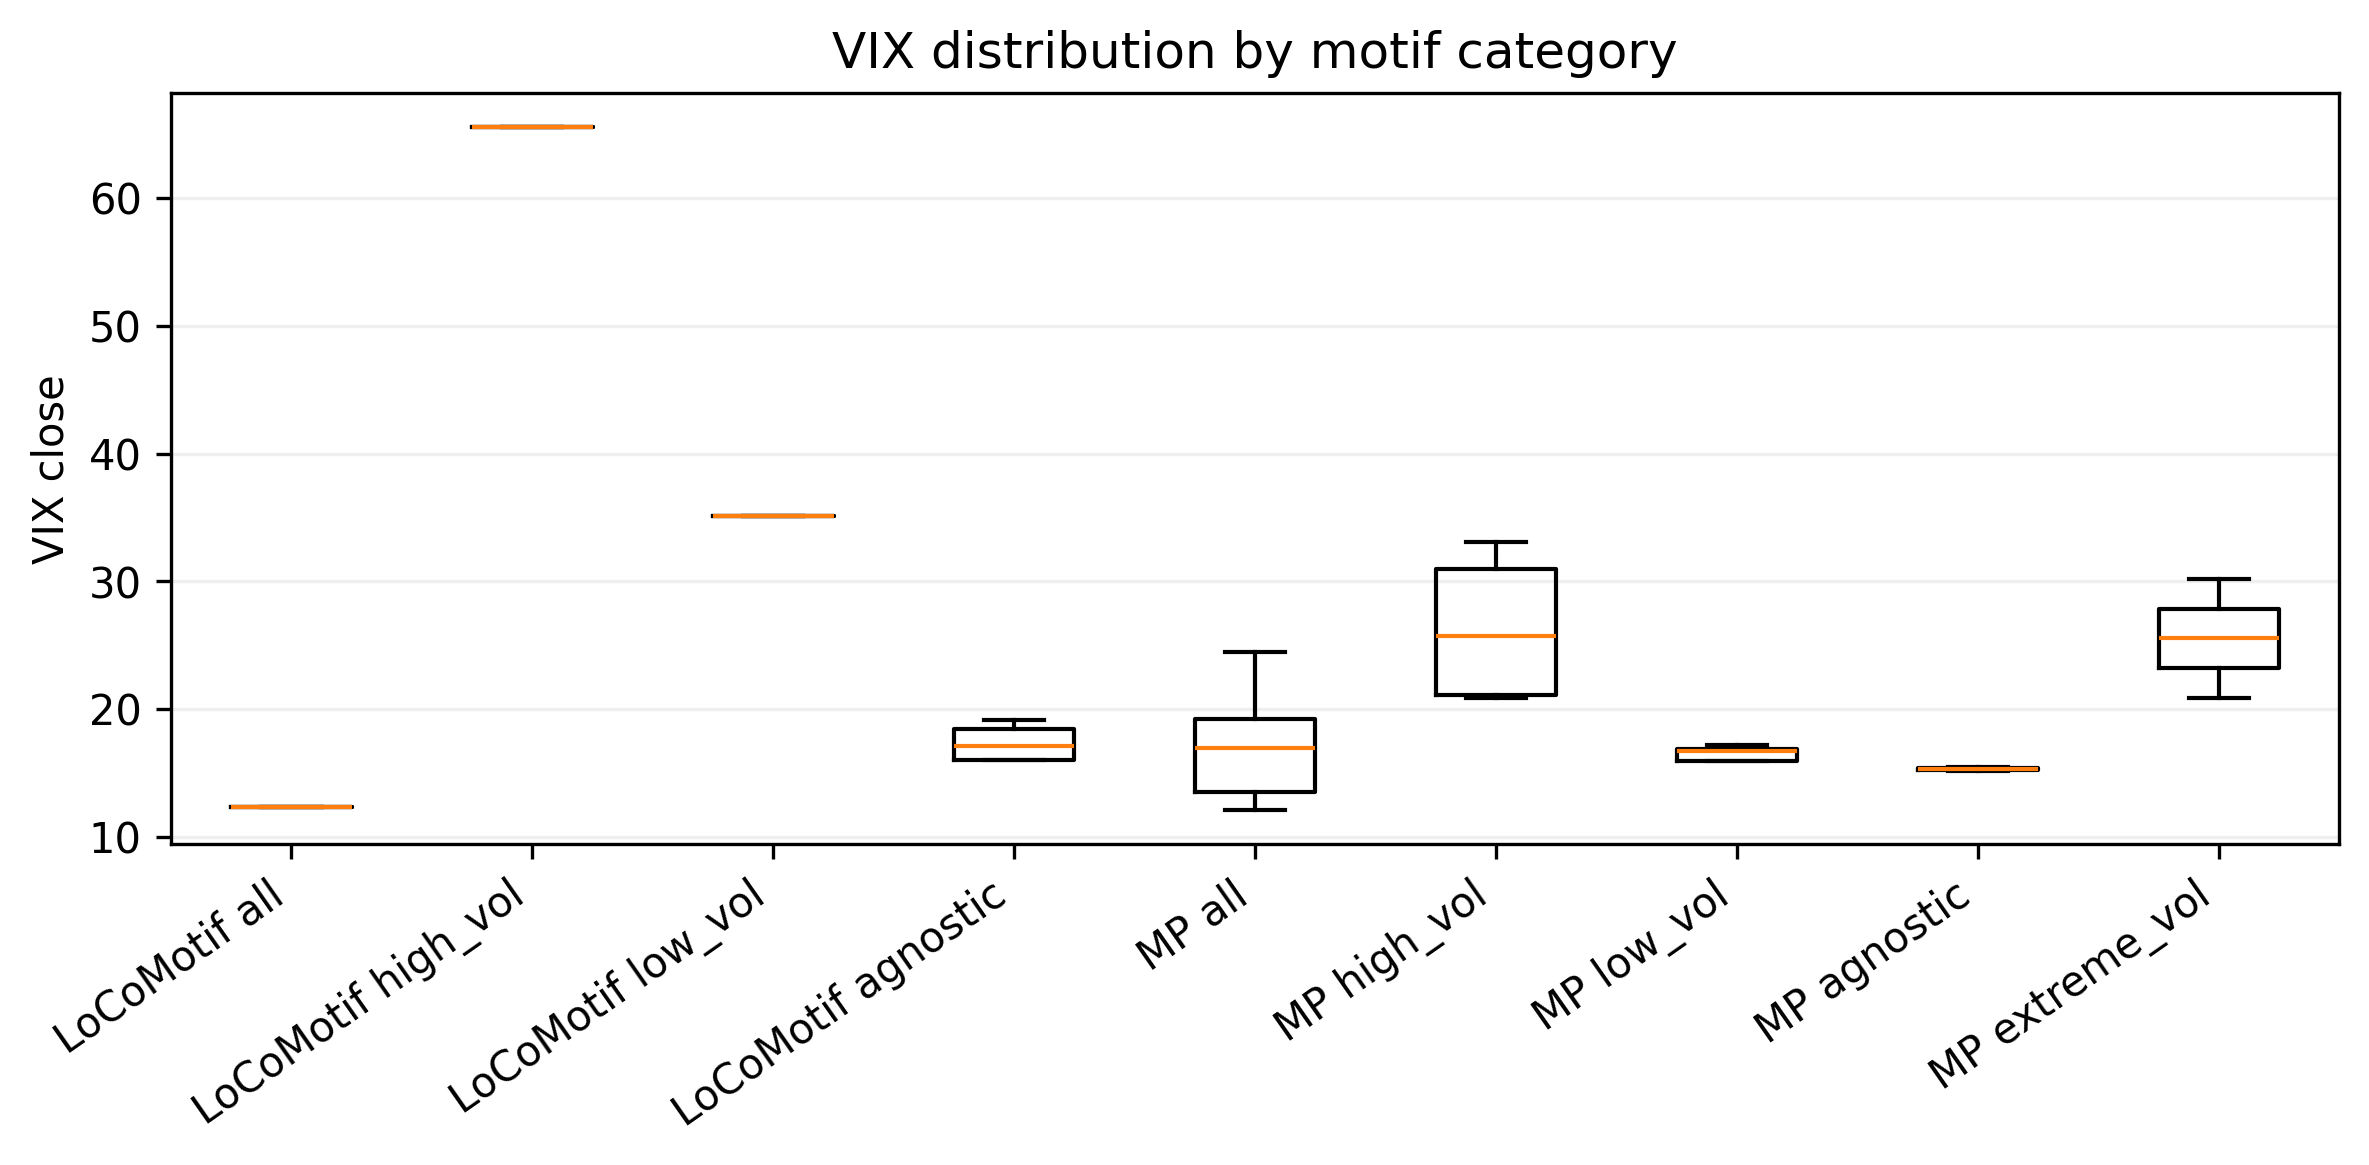
\includegraphics[width=0.9\linewidth]{reports/final_visual_evidence/figures/vix_distribution_by_motif_category.png}
\caption{vix distribution by motif category. VIX is external market-stress context only and is not used as a motif-discovery label.}
\end{figure}

\begin{figure}[ht]
\centering
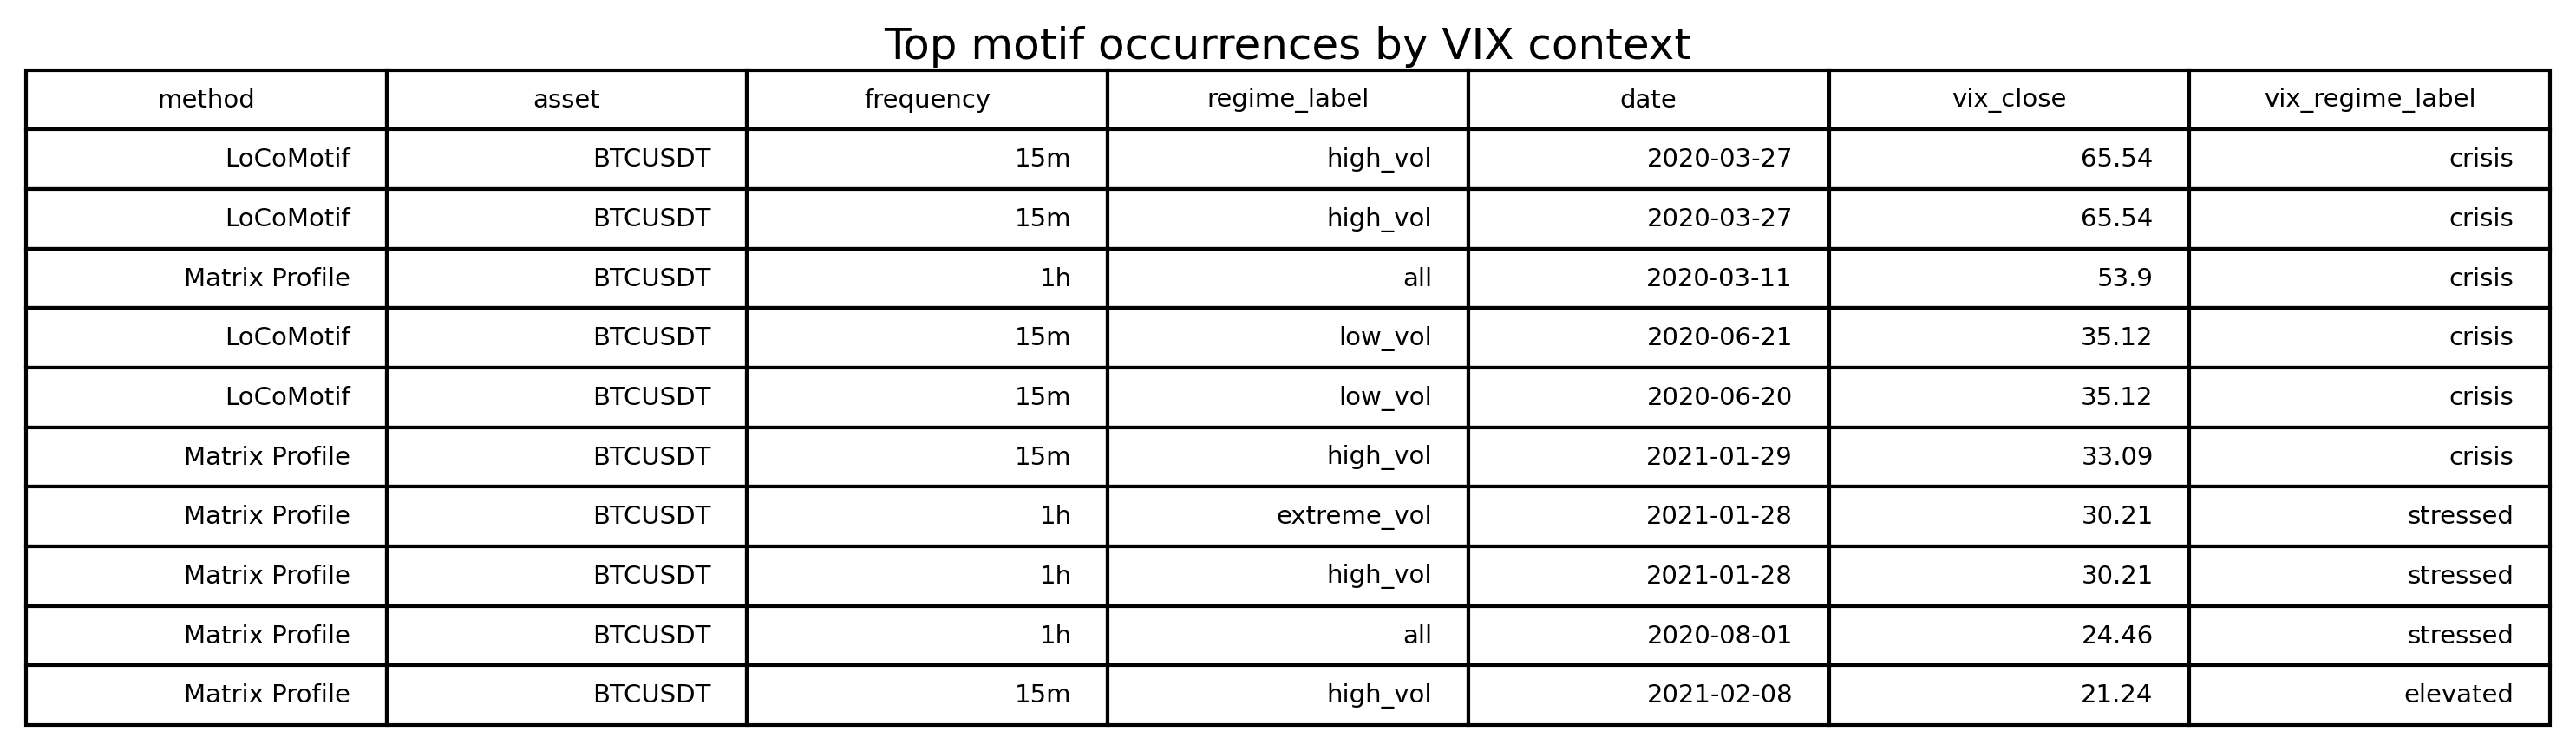
\includegraphics[width=0.9\linewidth]{reports/final_visual_evidence/figures/vix_event_context_top_motifs.png}
\caption{vix event context top motifs. VIX is external market-stress context only and is not used as a motif-discovery label.}
\end{figure}

\begin{figure}[ht]
\centering
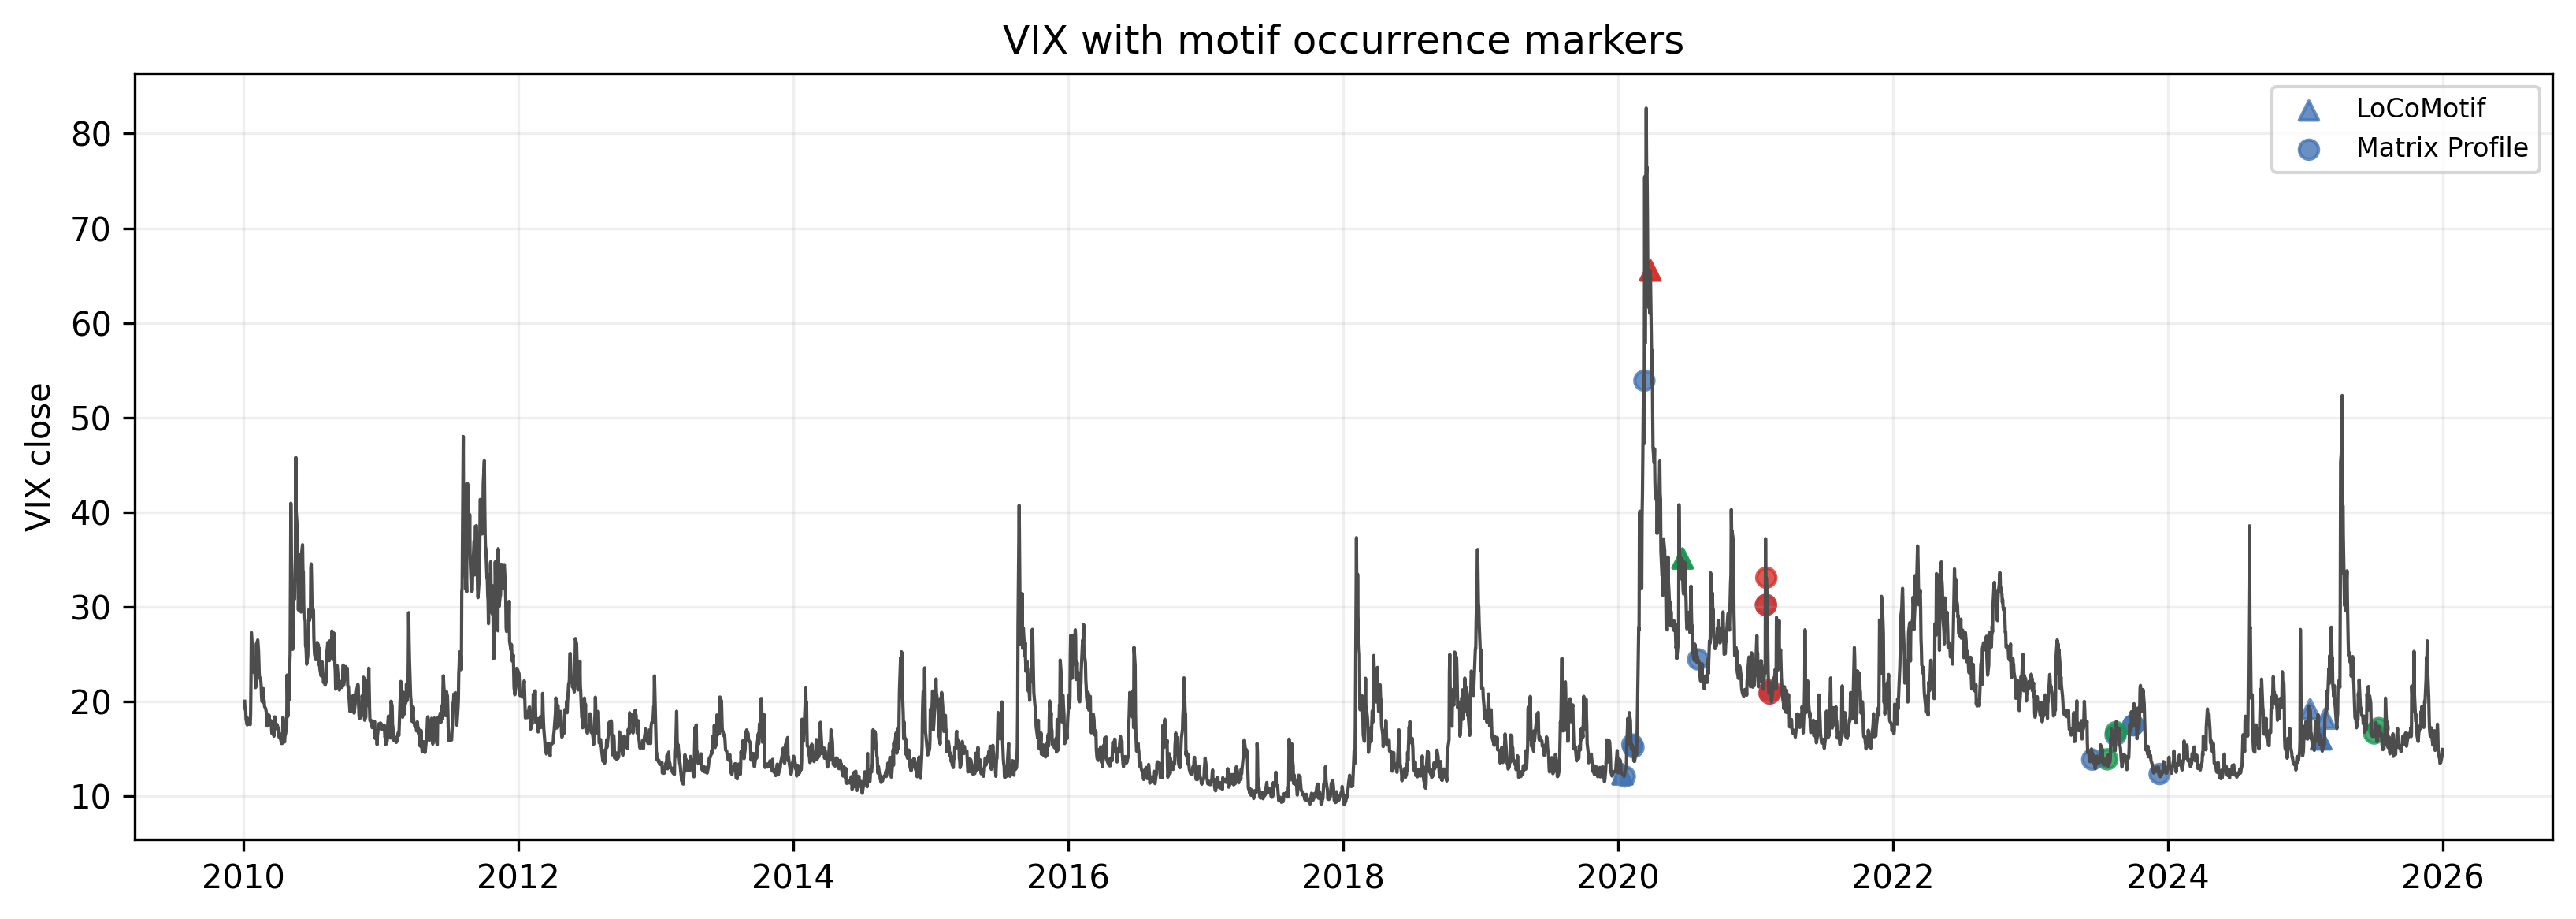
\includegraphics[width=0.9\linewidth]{reports/final_visual_evidence/figures/vix_with_motif_occurrence_markers.png}
\caption{vix with motif occurrence markers. VIX is external market-stress context only and is not used as a motif-discovery label.}
\end{figure}

